\documentclass[twoside]{book}

% Packages required by doxygen
\usepackage{fixltx2e}
\usepackage{calc}
\usepackage{doxygen}
\usepackage[export]{adjustbox} % also loads graphicx
\usepackage{graphicx}
\usepackage[utf8]{inputenc}
\usepackage{makeidx}
\usepackage{multicol}
\usepackage{multirow}
\PassOptionsToPackage{warn}{textcomp}
\usepackage{textcomp}
\usepackage[nointegrals]{wasysym}
\usepackage[table]{xcolor}

% Font selection
\usepackage[T1]{fontenc}
\usepackage[scaled=.90]{helvet}
\usepackage{courier}
\usepackage{amssymb}
\usepackage{sectsty}
\renewcommand{\familydefault}{\sfdefault}
\allsectionsfont{%
  \fontseries{bc}\selectfont%
  \color{darkgray}%
}
\renewcommand{\DoxyLabelFont}{%
  \fontseries{bc}\selectfont%
  \color{darkgray}%
}
\newcommand{\+}{\discretionary{\mbox{\scriptsize$\hookleftarrow$}}{}{}}

% Page & text layout
\usepackage{geometry}
\geometry{%
  a4paper,%
  top=2.5cm,%
  bottom=2.5cm,%
  left=2.5cm,%
  right=2.5cm%
}
\tolerance=750
\hfuzz=15pt
\hbadness=750
\setlength{\emergencystretch}{15pt}
\setlength{\parindent}{0cm}
\setlength{\parskip}{0.2cm}
\makeatletter
\renewcommand{\paragraph}{%
  \@startsection{paragraph}{4}{0ex}{-1.0ex}{1.0ex}{%
    \normalfont\normalsize\bfseries\SS@parafont%
  }%
}
\renewcommand{\subparagraph}{%
  \@startsection{subparagraph}{5}{0ex}{-1.0ex}{1.0ex}{%
    \normalfont\normalsize\bfseries\SS@subparafont%
  }%
}
\makeatother

% Headers & footers
\usepackage{fancyhdr}
\pagestyle{fancyplain}
\fancyhead[LE]{\fancyplain{}{\bfseries\thepage}}
\fancyhead[CE]{\fancyplain{}{}}
\fancyhead[RE]{\fancyplain{}{\bfseries\leftmark}}
\fancyhead[LO]{\fancyplain{}{\bfseries\rightmark}}
\fancyhead[CO]{\fancyplain{}{}}
\fancyhead[RO]{\fancyplain{}{\bfseries\thepage}}
\fancyfoot[LE]{\fancyplain{}{}}
\fancyfoot[CE]{\fancyplain{}{}}
\fancyfoot[RE]{\fancyplain{}{\bfseries\scriptsize Generated on Sun Apr 3 2016 13\+:22\+:13 for Unit Conversion and Dimensional Analysis Library by Doxygen }}
\fancyfoot[LO]{\fancyplain{}{\bfseries\scriptsize Generated on Sun Apr 3 2016 13\+:22\+:13 for Unit Conversion and Dimensional Analysis Library by Doxygen }}
\fancyfoot[CO]{\fancyplain{}{}}
\fancyfoot[RO]{\fancyplain{}{}}
\renewcommand{\footrulewidth}{0.4pt}
\renewcommand{\chaptermark}[1]{%
  \markboth{#1}{}%
}
\renewcommand{\sectionmark}[1]{%
  \markright{\thesection\ #1}%
}

% Indices & bibliography
\usepackage{natbib}
\usepackage[titles]{tocloft}
\setcounter{tocdepth}{3}
\setcounter{secnumdepth}{5}
\makeindex

% Hyperlinks (required, but should be loaded last)
\usepackage{ifpdf}
\ifpdf
  \usepackage[pdftex,pagebackref=true]{hyperref}
\else
  \usepackage[ps2pdf,pagebackref=true]{hyperref}
\fi
\hypersetup{%
  colorlinks=true,%
  linkcolor=blue,%
  citecolor=blue,%
  unicode%
}

% Custom commands
\newcommand{\clearemptydoublepage}{%
  \newpage{\pagestyle{empty}\cleardoublepage}%
}


%===== C O N T E N T S =====

\begin{document}

% Titlepage & ToC
\hypersetup{pageanchor=false,
             bookmarks=true,
             bookmarksnumbered=true,
             pdfencoding=unicode
            }
\pagenumbering{roman}
\begin{titlepage}
\vspace*{7cm}
\begin{center}%
{\Large Unit Conversion and Dimensional Analysis Library \\[1ex]\large 2.\+0.\+0 }\\
\vspace*{1cm}
{\large Generated by Doxygen 1.8.9.1}\\
\vspace*{0.5cm}
{\small Sun Apr 3 2016 13:22:13}\\
\end{center}
\end{titlepage}
\clearemptydoublepage
\tableofcontents
\clearemptydoublepage
\pagenumbering{arabic}
\hypersetup{pageanchor=true}

%--- Begin generated contents ---
\chapter{Main Page}
\label{index}\hypertarget{index}{}a compile-\/time, header-\/only, unit conversion library built on c++14 with no dependencies.

\subsection*{Latest Release -\/ v2.\+0.\+0 }

New features\+:
\begin{DoxyItemize}
\item Compile-\/time unit arithmetic via {\ttfamily unit\+\_\+value\+\_\+t}
\item Unit-\/enabled ports of most {\ttfamily $<$cmath$>$} functions, including c++11 extensions.
\item Square-\/root manipulators for {\ttfamily unit}, {\ttfamily unit\+\_\+t}, and {\ttfamily unit\+\_\+value\+\_\+t}
\item Improved documentation
\end{DoxyItemize}

Tested on\+:
\begin{DoxyItemize}
\item gcc -\/4.\+9
\item msvc2013
\item msvc2015
\end{DoxyItemize}

\href{https://github.com/nholthaus/units/releases/tag/v2.0.0}{\tt Download units v2.\+0.\+0}

\subsection*{Documentation }

The full documentation is available $\ast$\href{http://nholthaus.github.io/units}{\tt here}$\ast$.

\subsection*{Description }

The library consists of a single file (\hyperlink{units_8h}{include/units.\+h}), plus unit tests. To incorporate the library into your project, simply copy the header into a location in your include path. A C\+Make project is included to build the unit tests and documentation if desired.

The library provides a set of types, containers, and traits to solve dimensional analysis problems, that is, problems involving dimensioned physical quantities. The conversions between units are defined as ratios at compile time, making the library {\itshape incredibly} fast. Additionally, specifying units as {\itshape types}, rather than variable suffixes (or not at all), provides complete type-\/safety within the compiler. This means that code that accidently misuses units or which has errors in the dimensional analysis {\itshape will fail at compile-\/time, not at run-\/time}.

The unit test file {\ttfamily unit\+Tests/main.\+cpp} contains example usage of every type, trait, and function contained in the library, and while not exactly user-\/friendly, can be a valuable resource.

\subsection*{Unit tags }

Unit tags are the foundation of the unit library. Unit tags are types which are never instantiated in user code, but which provide the meta-\/information about different units, including how to convert between them, and how to determine their compatibility for conversion.

All unit tags are defined in namespaces under the {\ttfamily units} namespace, such as {\ttfamily \hyperlink{namespaceunits_1_1length}{units\+::length}} or {\ttfamily \hyperlink{namespaceunits_1_1angle}{units\+::angle}}, to avoid name clashes between units of different physical quantities which share the same names (like pounds). S\+I base units are defined as \char`\"{}categories\char`\"{} in the {\ttfamily unit} namespace.

Units are defined in terms of
\begin{DoxyEnumerate}
\item A scale factor relative to a base unit type.
\item A base unit
\item \mbox{[}optionally\mbox{]} a scale factor of {\ttfamily pi}
\item \mbox{[}optionally\mbox{]} a datum translation (such as the +/-\/ 32 required to convert between {\ttfamily fahrenheit} and {\ttfamily celsius})
\end{DoxyEnumerate}

All units have their origin in the Scientific International (S\+I) base unit system. A special exception is made for angle units, which are defined in S\+I as ( m $\ast$ m$^\wedge$-\/1), which is not {\itshape exactly} the same as dimensionless/scalar units for practical purposes (and probably why the S\+I didn\textquotesingle{}t define them as simple scalar units), and so in this library they are treated as a basic unit type.

{\itshape Example}\+: the defintions of some common length units are\+: \begin{DoxyVerb}namespace length
{
    using meters = units::unit<std::ratio<1>, units::category::length_unit>;    // meters are (1) unit of length in the SI system.
    using feet = units::unit<std::ratio<381, 1250>, meters>;                    // feet are 3.28084 meters.
}
\end{DoxyVerb}


\subsection*{Unit containers }

Unit containers are the workhorse of the units libary, and the primary classes which will be instantiated in user code. Containers are derived from the {\ttfamily unit\+\_\+t} class, and have the form {\ttfamily \mbox{[}unitname\mbox{]}\+\_\+t}, e.\+g. {\ttfamily meter\+\_\+t} or {\ttfamily radian\+\_\+t}. Containers are effectively doubles with associated unit type tags, and can be used wherever a double would be used to store a dimensioned quantity.

Unit containers are defined in terms of the units they represent, their underlying type, and an optional non-\/linear scale (think decibels or richter scale). For example, {\ttfamily meter\+\_\+t} would be defined\+: \begin{DoxyVerb}using meter_t = units::unit_t<units::length::meter, double, units::linear_scale>
\end{DoxyVerb}


or simply \begin{DoxyVerb}using meter_t = units::unit_t<units::length::meter>
\end{DoxyVerb}


since the underlying type and scale parameters default to {\ttfamily double} and {\ttfamily linear\+\_\+scale} respectively.

Units of compatible types (e.\+g length units) can be implicitely converted/assigned to one another. Units (with the exception of dimensionless types) cannot be implicitely converted to/from built-\/in types, such as {\ttfamily double}.

Units are constructed from built-\/in types, and the {\ttfamily to\+Double()} method (or {\ttfamily operator()}) can be used to retrieve a built-\/in type value. That said, the user should prefer to operate within the unit type-\/space as much as is practical, and wrappers of most {\ttfamily $<$cmath$>$} functions are provided to enable operating soly in the {\ttfamily unit\+\_\+t} domain.

The primary purpose of unit containers is to provide type safety and dimensional analysis for mathematical operations. for instance, the velocity of an object can be calculated\+: \begin{DoxyVerb}auto objectVelocity = units::meter_t(100.0) / units::second_t(2.0);
\end{DoxyVerb}


The resulting velocity type will be deduced to be {\ttfamily velocity\+::meters\+\_\+per\+\_\+second} with a value of 50.\+0. Additionally, if the return type if specified, the type system wll verify that the units are compatible. For example, the following will fail to compile\+: \begin{DoxyVerb}units::velocity::meters_per_second objectVelocity = units::square_meter_t(100.0) / units::second_t(2.0); // Error: Unit types are not compatible.`
\end{DoxyVerb}


Unit containers can (and should!) be used to perform implicit conversions\+: \begin{DoxyVerb}units::time::second_t a;
units::time::minute_t b(1.0);

a = b;  // a == 60.0
\end{DoxyVerb}


Arithmetic can be performed on unit containers the same way it can for built-\/in types. However, unlike built-\/in types, the return value of unit-\/type arithmetic will be the proper unit to represent the resulting quantity. \begin{DoxyVerb}using namespace units::length;
using namespace units::area;

meter_t a_m(1.0), b_m(2.0), c_m;
foot_t  a_ft(1.0), b_ft(2.0), c_ft;

c_m = a_m + b_m;                            // OK. c == 3m
c_ft = a_m + b_m;                           // OK. resulting 3m is converted to ft.
auto result = a_m * b_ft;                   // OK. result is `meter_t` (left-most unit)

auto result_sm = a_m * b_m;                 // OK. result_sm is `square_meter_t`.
auto result_s = a_m / b_m;                  // OK. result_s is `dimensionless_t`.
auto result = a_m * b_ft;                   // OK. result is `square_meter_t` (left-most unit)

auto result = a_m * square_meter_t(1.0);    // OK. units can always be multiplied. Result is `cubed<meter_t>`.
auto result = a_m * scalar_t(1.0);          // OK. units can always be multiplied. Result is `meter_t`.
\end{DoxyVerb}


Unsupported arithmetic, or improper return types will result in compiler errors\+: \begin{DoxyVerb}c_m = a_m + 5.0;                            // Error. can't add scalars to dimensioned units.
c_m = a_m + scalar_t(5.0);                  // Error. can't add scalars to dimensioned units.
auto result = a_m + square_meter_t(1.0);    // Error. Incompatible units.
\end{DoxyVerb}


By providing explicit return types for unit functions, the compiler can be used to verify the accuracy of the dimensional analysis, and thus avoiding costly errors.

\subsection*{{\ttfamily $<$cmath$>$} Functions }

The {\ttfamily units} library include type-\/safe unit\+\_\+t container wrappers for almost all of the $<$cmath$>$ functions, {\itshape including} the c++11 extensions. These functions can be found in the {\ttfamily \hyperlink{namespaceunits_1_1math}{units\+::math}} namespace. The {\ttfamily units} library versions don\textquotesingle{}t conflict with $<$cmath$>$, and it\textquotesingle{}s possible to use both libraries in the same code.

The overloaded functions ensure that only the proper unit types are accepted into the functions, and that the return value type matches the expected units, all without needing to result to the type-\/unsafe {\ttfamily to\+Double()} member.

In {\itshape rare} cases, the overload resolution for a given type may be ambiguous. If so, simply preprend the function with the fully-\/qualified {\ttfamily \hyperlink{namespaceunits_1_1math}{units\+::math}} prefix, e.\+g. \begin{DoxyVerb}meter_t x(2.0);
meter_t y(3.0);
square_meter_t z(1.0);
square_meter_t result;

result = fma(x, y, z);                                              // Error: ambiguous
double result = fma(x.toDouble(), y.toDouble(), z.toDouble());      // Warning: Unsafe!
result = math::fma(x, y, z);                                        // OK.
\end{DoxyVerb}


\subsection*{Exponentials and Square Roots }

Many functions require units to be raised to some power. This can be accomplished using the {\ttfamily \hyperlink{namespaceunits_1_1math_adf689b7864a5c78a00628574cc8dca6b}{units\+::math\+::pow}} function\+: \begin{DoxyVerb}square_meter_t m2 = units::math::pow<2>(meter_t(5.0));  // m2 == 25.0
\end{DoxyVerb}


The only constraint is that the exponential power (given in the template argument) must be known at compile time, so that the type system can deduce the output type. This differs from the {\ttfamily $<$cmath$>$ pow} implementation, which takes exponent values at runtime.

Square roots are also provided with the {\ttfamily \hyperlink{group___unit_math_gabfa4684a203331f788cf8294fdc25c7a}{units\+::math\+::sqrt}} function. Due to the nature of the {\ttfamily sqrt} operation, the units library can often provide exact conversions for square root operations, but {\itshape not in every case}. The rest of the time, the {\ttfamily sqrt} unit will be a {\itshape rational\+\_\+approximation} of the real value. These are guaranteed to be accurate to at least 10 decimal places. \begin{DoxyVerb}meter_t m = units::math::sqrt(square_meter_t(4.0));     // m == 2.0
\end{DoxyVerb}


\subsection*{Efficiency }

Complex, recurively-\/defined conversions are performed in just 5 instructions\+: \begin{DoxyVerb}    year_t twoYears(2.0);
    week_t twoYearsInWeeks = twoYears;
00007FF7BDB57FF6  xorps       xmm9,xmm9  
00007FF7BDB57FFA  cvtsi2sd    xmm9,rax  
00007FF7BDB57FFF  mulsd       xmm9,mmword ptr [__real@4000000000000000 (07FF7BDBB31A0h)]  
00007FF7BDB58008  divsd       xmm9,mmword ptr [__real@401c000000000000 (07FF7BDBB33C0h)]  
00007FF7BDB58011  movsd       mmword ptr [rbp+6Fh],xmm9  
    EXPECT_EQ(week_t(104.286), twoYearsInWeeks);
00007FF7BDB58017  ...
\end{DoxyVerb}


In the library, the year to week conversion is defined in terms of {\ttfamily years -\/$>$ days -\/$>$ hours -\/$>$ minutes -\/$>$ seconds -\/$>$ minutes -\/$>$ hours -\/$>$ days -\/$>$ weeks} but the total conversion ratio is computed at compile-\/time and the math is optimized to two floating-\/point operations.

Unit conversions between equivalent types are optimized away completely, and generate {\itshape no machine code}.

\subsection*{Compile-\/time Unit Manipulation }

In many cases, unit equations are used to determine derived values from a set of values which are known at comile-\/time. In these situations, it would be optimal to pre-\/compute the derived values {\itshape at compile time}, thus generating no machine code and incurring no run-\/time penalty.

The {\ttfamily unit\+\_\+value\+\_\+t} class is the mechanism in the units library to perform compule-\/time arithmetic. The {\ttfamily unit\+\_\+value\+\_\+t} class functions exactly the same way as {\ttfamily std\+::ratio}, but with an associated unit tag and the ensuing type safety.

For a simple example, let\textquotesingle{}s define a right triangle whose hypotnuse is the sum of the squares of its side (a pythagorean triple) \begin{DoxyVerb}struct RightTriangle
{
    using a = unit_value_t<meters, 3>;
    using b = unit_value_t<meters, 4>;
    using c = unit_value_sqrt<unit_value_add<unit_value_power<a, 2>, unit_value_power<b, 2>>>;
};
\end{DoxyVerb}


The definition above is perfectly efficient, as it generates {\itshape no run-\/time code} whatsoever, and still provides all the type safety of unit containers. The values of {\ttfamily a}, {\ttfamily b}, and {\ttfamily c} can be accessed at runtime using the static {\ttfamily value()} method of {\ttfamily unit\+\_\+value\+\_\+t} \begin{DoxyVerb}auto a = RightTriangle::a::value(); // a is `meter_t(3)`
auto b = RightTriangle::b::value(); // b is `meter_t(4)`
auto c = RightTriangle::c::value(); // c is `meter_t(5)`
\end{DoxyVerb}


The available compile-\/time operations are\+:
\begin{DoxyItemize}
\item {\ttfamily \hyperlink{structunits_1_1unit__value__add}{units\+::unit\+\_\+value\+\_\+add}}
\item {\ttfamily \hyperlink{structunits_1_1unit__value__subtract}{units\+::unit\+\_\+value\+\_\+subtract}}
\item {\ttfamily \hyperlink{structunits_1_1unit__value__multiply}{units\+::unit\+\_\+value\+\_\+multiply}}
\item {\ttfamily \hyperlink{structunits_1_1unit__value__divide}{units\+::unit\+\_\+value\+\_\+divide}}
\item {\ttfamily \hyperlink{structunits_1_1unit__value__power}{units\+::unit\+\_\+value\+\_\+power}}
\item {\ttfamily \hyperlink{structunits_1_1unit__value__sqrt}{units\+::unit\+\_\+value\+\_\+sqrt}}
\end{DoxyItemize}

\subsection*{Conversion without unit containers }

The preferred method of conversion is implicitly though the use of unit containers, however unit conversion can be accomplished using {\ttfamily \hyperlink{group___conversion_gae7541dbcd66420e011c82ac58ef7723c}{units\+::convert}} for arithmetic types\+: \begin{DoxyVerb}double val_in = convert<feet, inches>(1.0); // val_in == 12.0
\end{DoxyVerb}


For type-\/safe conversion, prefer implicit conversion via unit\+\_\+t type containers..

\subsection*{Namespaces }

Unit tags and containers are split into separate namespaces to avoid conflicting unit names which represent different physical quantities.

Unit tag and unit\+\_\+t container definitions are defined in the following namespaces\+:
\begin{DoxyItemize}
\item \hyperlink{namespaceunits_1_1length}{units\+::length}
\item \hyperlink{namespaceunits_1_1mass}{units\+::mass}
\item \hyperlink{namespaceunits_1_1time}{units\+::time}
\item \hyperlink{namespaceunits_1_1angle}{units\+::angle} (plane)
\item \hyperlink{namespaceunits_1_1current}{units\+::current}
\item \hyperlink{namespaceunits_1_1temperature}{units\+::temperature}
\item \hyperlink{namespaceunits_1_1substance}{units\+::substance} (amount of, i.\+e. moles)
\item \hyperlink{namespaceunits_1_1luminous__intensity}{units\+::luminous\+\_\+intensity}
\item \hyperlink{namespaceunits_1_1solid__angle}{units\+::solid\+\_\+angle}
\item \hyperlink{namespaceunits_1_1frequency}{units\+::frequency}
\item \hyperlink{namespaceunits_1_1velocity}{units\+::velocity}
\item \hyperlink{namespaceunits_1_1angular__velocity}{units\+::angular\+\_\+velocity}
\item \hyperlink{namespaceunits_1_1acceleration}{units\+::acceleration}
\item \hyperlink{namespaceunits_1_1force}{units\+::force}
\item \hyperlink{namespaceunits_1_1pressure}{units\+::pressure}
\item \hyperlink{namespaceunits_1_1charge}{units\+::charge}
\item \hyperlink{namespaceunits_1_1energy}{units\+::energy}
\item \hyperlink{namespaceunits_1_1power}{units\+::power}
\item \hyperlink{namespaceunits_1_1voltage}{units\+::voltage}
\item \hyperlink{namespaceunits_1_1capacitance}{units\+::capacitance}
\item \hyperlink{namespaceunits_1_1impedance}{units\+::impedance}
\item \hyperlink{namespaceunits_1_1magnetic__flux}{units\+::magnetic\+\_\+flux}
\item \hyperlink{namespaceunits_1_1magnetic__field__strength}{units\+::magnetic\+\_\+field\+\_\+strength}
\item \hyperlink{namespaceunits_1_1inductance}{units\+::inductance}
\item \hyperlink{namespaceunits_1_1luminous__flux}{units\+::luminous\+\_\+flux}
\item \hyperlink{namespaceunits_1_1illuminance}{units\+::illuminance}
\item \hyperlink{namespaceunits_1_1radiation}{units\+::radiation}
\item \hyperlink{namespaceunits_1_1torque}{units\+::torque}
\item \hyperlink{namespaceunits_1_1area}{units\+::area}
\item \hyperlink{namespaceunits_1_1volume}{units\+::volume}
\item \hyperlink{namespaceunits_1_1density}{units\+::density}
\item \hyperlink{namespaceunits_1_1concentration}{units\+::concentration}
\item \hyperlink{namespaceunits_1_1constants}{units\+::constants} (scalar and non-\/scalar physical constants like Avagadro\textquotesingle{}s number)
\end{DoxyItemize}

Mathematical operations like {\ttfamily sin}, {\ttfamily log}, {\ttfamily floor}, etc are defined in the following namespaces\+:
\begin{DoxyItemize}
\item \hyperlink{namespaceunits_1_1math}{units\+::math}
\end{DoxyItemize}

Type traits that you can use to test unit types are defined in the following namespaces\+:
\begin{DoxyItemize}
\item \hyperlink{namespaceunits_1_1traits}{units\+::traits}
\end{DoxyItemize}

\subsection*{Defining new units }

The units library strives to provide built-\/in types for every conceievable unit, and before defing your own units you should double-\/check the namespaces to make sure it\textquotesingle{}s not already included. That said, if you need to roll your own units, the library is extensible by design.

Defining new units is simple, as they can be recursively defined as ratio of previously-\/defined units in a way that mimics natural language and is highly readable\+: \begin{DoxyVerb}namespace time
{
    using seconds = units::unit<std::ratio<1>,   units::category::time_unit>;
    using minutes = units::unit<std::ratio<60>,  seconds>;
    using hours   = units::unit<std::ratio<60>,  minutes>;
    using days    = units::unit<std::ratio<24>,  hours>;
    using weeks   = units::unit<std::ratio<7>,   days>;
    using years   = units::unit<std::ratio<365>, days>;
}
\end{DoxyVerb}


Units are defined in the form\+: {\ttfamily using \mbox{[}unit\mbox{]} = unit$<$std\+::ratio$<$\mbox{[}number of base units per unit\mbox{]}$>$, \mbox{[}base unit\mbox{]}$>$;}, where\+:
\begin{DoxyItemize}
\item the {\ttfamily \mbox{[}unit\mbox{]}} is what you are defining.
\item the {\ttfamily \mbox{[}base unit\mbox{]}} is the unit that {\ttfamily \mbox{[}unit\mbox{]}} will be defined in terms of, and
\item the {\ttfamily \mbox{[}number of base units per unit\mbox{]}} is the conversion ratio between the two, expressed as a {\ttfamily std\+::ratio} type.
\end{DoxyItemize}

Compound units are defined in a similar manner, with additional helper functions for polynomials\+: \begin{DoxyVerb}using acceleration = compound_unit<meters, inverse<squared<seconds>>>;      // (m / s^2)
\end{DoxyVerb}


The available helpers are\+:
\begin{DoxyItemize}
\item {\ttfamily \hyperlink{group___unit_manipulators_gaacc539ef162e24b260d023d3ff949b57}{units\+::inverse}$<$...$>$} (inverts the unit, e.\+g. meters becomes meters$^\wedge$-\/1, or 1 / meters)
\item {\ttfamily \hyperlink{group___unit_manipulators_ga636346f7898c35eb98a796bec1d77fb2}{units\+::squared}$<$...$>$} (squares the unit, e.\+g. meters becomes meters$^\wedge$2)
\item {\ttfamily \hyperlink{group___unit_manipulators_gad3e94dc693fe45a580b382cb666434a1}{units\+::cubed}$<$...$>$} (cubes the unit, e.\+g. meters becomes meters$^\wedge$3)
\item {\ttfamily \hyperlink{group___unit_manipulators_ga66c5d3d0e80c7c3e56683d7df366b380}{units\+::square\+\_\+root}$<$...$>$} (takes the square root of the unit, e.\+g meters$^\wedge$2 becomes meters)
\item {\ttfamily \hyperlink{group___unit_manipulators_ga8a7180c782263384a118dc8ffa5bc689}{units\+::atto}$<$...$>$} through {\ttfamily \hyperlink{group___unit_manipulators_gad0c18c5a47e0fe677715f0328f818515}{units\+::exa}$<$...$>$} metric prefixes
\end{DoxyItemize}

\subsection*{Unit Type Traits }

The units library provides a comprehensive set of type-\/traits, which can be used in templated user code to enforce that the unit types have certain properties.

For example, let\textquotesingle{}s say you want to write a function that validates that the square footage of an office (given in any units), meets the minimum size required by local ordinance. \begin{DoxyVerb}template<typename Units>
bool isMinimumSize(Units x)
{
    return x >= square_feet_t(80.0);
}
\end{DoxyVerb}


This function will fail to compile if {\ttfamily Units} is not a unit of area (since incompatible unit types are not comparable), but it will produce a series difficult-\/to-\/understand tempalte errors. Type traits could be used to make the error message more friendly\+: \begin{DoxyVerb}template<typename Units>
bool isMinimumSize(Units x)
{
    static_assert(units::traits::is_area_unit<Units>::value, "Input value x must represent an area quantity.");
    return x >= square_feet_t(80.0);
}
\end{DoxyVerb}


See the {\ttfamily \hyperlink{namespaceunits_1_1traits}{units\+::traits}} namespace for a list of all the suported traits.

\subsection*{Build Instructions }

The library itself consists of a single header (\hyperlink{units_8h}{include/units.\+h}), and can be included into your project without being built.

The unit tests and documentation can be built with C\+Make. A doxygen installation is required to generate the documentation, and a Tex install is needed if pdf documentation is desired.

To build the tests\+:

Windows\+:
\begin{DoxyEnumerate}
\item Ensure cmake is installed, and that the {\ttfamily bin} directory is in your P\+A\+T\+H\% variable, and that a compiler like {\ttfamily Visual Studio 2015 Community Edition} is installed.
\item clone the repository or download the {\ttfamily .zip} package.
\item Open a {\ttfamily cmd} terminal and navigate to the source directory.
\item Type the following commands\+:
\begin{DoxyItemize}
\item {\ttfamily md build}
\item {\ttfamily cd build}
\item {\ttfamily cmake -\/\+Wno-\/dev ..}
\item {\ttfamily cmake -\/-\/build . -\/-\/config Release}
\end{DoxyItemize}
\item The tests will be created in an executable called {\ttfamily unit\+Lib\+Test.\+exe} in the folder {\ttfamily build/unit\+Tests/\+Release}.
\end{DoxyEnumerate}

Linux\+:
\begin{DoxyEnumerate}
\item Ensure you are using cmake 3.\+2 or later. You can verify this with {\ttfamily cmake -\/-\/version}.
\item Ensure you are using gcc version 4.\+9 or greater. You can verify this with {\ttfamily gcc -\/-\/version}.
\item clone the repository or download the {\ttfamily .tar.\+gz} package.
\item Open a terminal and navigate to the source directory.
\item Type the following commands\+:
\begin{DoxyItemize}
\item {\ttfamily mkdir build}
\item {\ttfamily cd build}
\item {\ttfamily cmake -\/\+Wno-\/dev ..}
\item {\ttfamily cmake -\/-\/build . -\/-\/config Release}
\end{DoxyItemize}
\item The tests will be created in an executable called {\ttfamily unit\+Lib\+Test} in the folder {\ttfamily build/unit\+Tests}.
\end{DoxyEnumerate}

\subsection*{Previous Releases }


\begin{DoxyItemize}
\item v1.\+3.\+0 -\/ Adds ostream support. bug fixes. Tested with gcc-\/4.\+9.\+2, msvc2013, msvc2015.
\item v1.\+2.\+2 -\/ Bug fixes (\#1) and namespace cleanup. Tested with msvc2015, gcc 5.\+2.\+1
\item v1.\+2.\+0 -\/ Adds angular velocity units. Tested with gcc-\/4.\+9.\+2, msvc2013, msvc2015.
\item v1.\+1.\+1 -\/ Adds Doxygen and additional type traits. Tested with gcc-\/4.\+9.\+2, msvc2013, msvc2015.
\item v1.\+0.\+0 -\/ Initial release. Tested with msvc2015 
\end{DoxyItemize}
\chapter{Module Index}
\section{Modules}
Here is a list of all modules\+:\begin{DoxyCompactList}
\item \contentsline{section}{Unit Containers}{\pageref{group___unit_containers}}{}
\item \contentsline{section}{Unit Types}{\pageref{group___unit_types}}{}
\item \contentsline{section}{Unit Manipulators}{\pageref{group___unit_manipulators}}{}
\item \contentsline{section}{Compile-\/time Unit Manipulators}{\pageref{group___compile_time_unit_manipulators}}{}
\item \contentsline{section}{Unit Math}{\pageref{group___unit_math}}{}
\item \contentsline{section}{Explicit Conversion}{\pageref{group___conversion}}{}
\item \contentsline{section}{Type Traits}{\pageref{group___type_traits}}{}
\end{DoxyCompactList}

\chapter{Namespace Index}
\section{Namespace List}
Here is a list of all documented namespaces with brief descriptions\+:\begin{DoxyCompactList}
\item\contentsline{section}{\hyperlink{namespaceunits}{units} \\*Unit Conversion Library namespace }{\pageref{namespaceunits}}{}
\item\contentsline{section}{\hyperlink{namespaceunits_1_1acceleration}{units\+::acceleration} \\*Namespace for unit types and containers representing acceleration values }{\pageref{namespaceunits_1_1acceleration}}{}
\item\contentsline{section}{\hyperlink{namespaceunits_1_1angle}{units\+::angle} \\*Namespace for unit types and containers representing angle values }{\pageref{namespaceunits_1_1angle}}{}
\item\contentsline{section}{\hyperlink{namespaceunits_1_1angular__velocity}{units\+::angular\+\_\+velocity} \\*Namespace for unit types and containers representing angular velocity values }{\pageref{namespaceunits_1_1angular__velocity}}{}
\item\contentsline{section}{\hyperlink{namespaceunits_1_1area}{units\+::area} \\*Namespace for unit types and containers representing area values }{\pageref{namespaceunits_1_1area}}{}
\item\contentsline{section}{\hyperlink{namespaceunits_1_1capacitance}{units\+::capacitance} \\*Namespace for unit types and containers representing capacitance values }{\pageref{namespaceunits_1_1capacitance}}{}
\item\contentsline{section}{\hyperlink{namespaceunits_1_1category}{units\+::category} \\*Namespace representing the implemented base and derived unit types }{\pageref{namespaceunits_1_1category}}{}
\item\contentsline{section}{\hyperlink{namespaceunits_1_1charge}{units\+::charge} \\*Namespace for unit types and containers representing charge values }{\pageref{namespaceunits_1_1charge}}{}
\item\contentsline{section}{\hyperlink{namespaceunits_1_1concentration}{units\+::concentration} \\*Namespace for unit types and containers representing concentration values }{\pageref{namespaceunits_1_1concentration}}{}
\item\contentsline{section}{\hyperlink{namespaceunits_1_1conductance}{units\+::conductance} \\*Namespace for unit types and containers representing conductance values }{\pageref{namespaceunits_1_1conductance}}{}
\item\contentsline{section}{\hyperlink{namespaceunits_1_1constants}{units\+::constants} \\*Namespace for physical constants like P\+I and Avogadro\textquotesingle{}s Number }{\pageref{namespaceunits_1_1constants}}{}
\item\contentsline{section}{\hyperlink{namespaceunits_1_1current}{units\+::current} \\*Namespace for unit types and containers representing current values }{\pageref{namespaceunits_1_1current}}{}
\item\contentsline{section}{\hyperlink{namespaceunits_1_1density}{units\+::density} \\*Namespace for unit types and containers representing density values }{\pageref{namespaceunits_1_1density}}{}
\item\contentsline{section}{\hyperlink{namespaceunits_1_1dimensionless}{units\+::dimensionless} \\*Namespace for unit types and containers for units that have no dimension (scalar units) }{\pageref{namespaceunits_1_1dimensionless}}{}
\item\contentsline{section}{\hyperlink{namespaceunits_1_1energy}{units\+::energy} \\*Namespace for unit types and containers representing energy values }{\pageref{namespaceunits_1_1energy}}{}
\item\contentsline{section}{\hyperlink{namespaceunits_1_1force}{units\+::force} \\*Namespace for unit types and containers representing force values }{\pageref{namespaceunits_1_1force}}{}
\item\contentsline{section}{\hyperlink{namespaceunits_1_1frequency}{units\+::frequency} \\*Namespace for unit types and containers representing frequency values }{\pageref{namespaceunits_1_1frequency}}{}
\item\contentsline{section}{\hyperlink{namespaceunits_1_1illuminance}{units\+::illuminance} \\*Namespace for unit types and containers representing illuminance values }{\pageref{namespaceunits_1_1illuminance}}{}
\item\contentsline{section}{\hyperlink{namespaceunits_1_1impedance}{units\+::impedance} \\*Namespace for unit types and containers representing impedance values }{\pageref{namespaceunits_1_1impedance}}{}
\item\contentsline{section}{\hyperlink{namespaceunits_1_1inductance}{units\+::inductance} \\*Namespace for unit types and containers representing inductance values }{\pageref{namespaceunits_1_1inductance}}{}
\item\contentsline{section}{\hyperlink{namespaceunits_1_1length}{units\+::length} \\*Namespace for unit types and containers representing length values }{\pageref{namespaceunits_1_1length}}{}
\item\contentsline{section}{\hyperlink{namespaceunits_1_1luminous__flux}{units\+::luminous\+\_\+flux} \\*Namespace for unit types and containers representing \hyperlink{namespaceunits_1_1luminous__flux}{luminous\+\_\+flux} values }{\pageref{namespaceunits_1_1luminous__flux}}{}
\item\contentsline{section}{\hyperlink{namespaceunits_1_1luminous__intensity}{units\+::luminous\+\_\+intensity} \\*Namespace for unit types and containers representing \hyperlink{namespaceunits_1_1luminous__intensity}{luminous\+\_\+intensity} values }{\pageref{namespaceunits_1_1luminous__intensity}}{}
\item\contentsline{section}{\hyperlink{namespaceunits_1_1magnetic__field__strength}{units\+::magnetic\+\_\+field\+\_\+strength} \\*Namespace for unit types and containers representing \hyperlink{namespaceunits_1_1magnetic__field__strength}{magnetic\+\_\+field\+\_\+strength} values }{\pageref{namespaceunits_1_1magnetic__field__strength}}{}
\item\contentsline{section}{\hyperlink{namespaceunits_1_1magnetic__flux}{units\+::magnetic\+\_\+flux} \\*Namespace for unit types and containers representing \hyperlink{namespaceunits_1_1magnetic__flux}{magnetic\+\_\+flux} values }{\pageref{namespaceunits_1_1magnetic__flux}}{}
\item\contentsline{section}{\hyperlink{namespaceunits_1_1mass}{units\+::mass} \\*Namespace for unit types and containers representing mass values }{\pageref{namespaceunits_1_1mass}}{}
\item\contentsline{section}{\hyperlink{namespaceunits_1_1math}{units\+::math} \\*Namespace for unit-\/enabled versions of the {\ttfamily $<$cmath$>$} library }{\pageref{namespaceunits_1_1math}}{}
\item\contentsline{section}{\hyperlink{namespaceunits_1_1power}{units\+::power} \\*Namespace for unit types and containers representing power values }{\pageref{namespaceunits_1_1power}}{}
\item\contentsline{section}{\hyperlink{namespaceunits_1_1pressure}{units\+::pressure} \\*Namespace for unit types and containers representing pressure values }{\pageref{namespaceunits_1_1pressure}}{}
\item\contentsline{section}{\hyperlink{namespaceunits_1_1radiation}{units\+::radiation} \\*Namespace for unit types and containers representing radiation values }{\pageref{namespaceunits_1_1radiation}}{}
\item\contentsline{section}{\hyperlink{namespaceunits_1_1solid__angle}{units\+::solid\+\_\+angle} \\*Namespace for unit types and containers representing \hyperlink{namespaceunits_1_1solid__angle}{solid\+\_\+angle} values }{\pageref{namespaceunits_1_1solid__angle}}{}
\item\contentsline{section}{\hyperlink{namespaceunits_1_1substance}{units\+::substance} \\*Namespace for unit types and containers representing substance values }{\pageref{namespaceunits_1_1substance}}{}
\item\contentsline{section}{\hyperlink{namespaceunits_1_1temperature}{units\+::temperature} \\*Namespace for unit types and containers representing temperature values }{\pageref{namespaceunits_1_1temperature}}{}
\item\contentsline{section}{\hyperlink{namespaceunits_1_1time}{units\+::time} \\*Namespace for unit types and containers representing time values }{\pageref{namespaceunits_1_1time}}{}
\item\contentsline{section}{\hyperlink{namespaceunits_1_1torque}{units\+::torque} \\*Namespace for unit types and containers representing torque values }{\pageref{namespaceunits_1_1torque}}{}
\item\contentsline{section}{\hyperlink{namespaceunits_1_1traits}{units\+::traits} \\*Namespace representing type traits which can access the properties of types provided by the units library }{\pageref{namespaceunits_1_1traits}}{}
\item\contentsline{section}{\hyperlink{namespaceunits_1_1velocity}{units\+::velocity} \\*Namespace for unit types and containers representing velocity values }{\pageref{namespaceunits_1_1velocity}}{}
\item\contentsline{section}{\hyperlink{namespaceunits_1_1voltage}{units\+::voltage} \\*Namespace for unit types and containers representing voltage values }{\pageref{namespaceunits_1_1voltage}}{}
\item\contentsline{section}{\hyperlink{namespaceunits_1_1volume}{units\+::volume} \\*Namespace for unit types and containers representing volume values }{\pageref{namespaceunits_1_1volume}}{}
\end{DoxyCompactList}

\chapter{Hierarchical Index}
\section{Class Hierarchy}
This inheritance list is sorted roughly, but not completely, alphabetically\+:\begin{DoxyCompactList}
\item \+\_\+base\+\_\+unit\+\_\+t\begin{DoxyCompactList}
\item \contentsline{section}{units\+:\+:base\+\_\+unit$<$ Meter, Kilogram, Second, Radian, Ampere, Kelvin, Mole, Candela $>$}{\pageref{structunits_1_1base__unit}}{}
\end{DoxyCompactList}
\item \+\_\+unit\begin{DoxyCompactList}
\item \contentsline{section}{units\+:\+:unit$<$ Conversion, Base\+Unit, Pi\+Exponent, Translation $>$}{\pageref{structunits_1_1unit}}{}
\end{DoxyCompactList}
\item \+\_\+unit\+\_\+t\begin{DoxyCompactList}
\item \contentsline{section}{units\+:\+:unit\+\_\+t$<$ Units, T, Non\+Linear\+Scale $>$}{\pageref{classunits_1_1unit__t}}{}
\end{DoxyCompactList}
\item \+\_\+unit\+\_\+value\+\_\+t\begin{DoxyCompactList}
\item \contentsline{section}{units\+:\+:unit\+\_\+value\+\_\+add$<$ U1, U2 $>$}{\pageref{structunits_1_1unit__value__add}}{}
\item \contentsline{section}{units\+:\+:unit\+\_\+value\+\_\+divide$<$ U1, U2 $>$}{\pageref{structunits_1_1unit__value__divide}}{}
\item \contentsline{section}{units\+:\+:unit\+\_\+value\+\_\+multiply$<$ U1, U2 $>$}{\pageref{structunits_1_1unit__value__multiply}}{}
\item \contentsline{section}{units\+:\+:unit\+\_\+value\+\_\+power$<$ U1, power $>$}{\pageref{structunits_1_1unit__value__power}}{}
\item \contentsline{section}{units\+:\+:unit\+\_\+value\+\_\+sqrt$<$ U1, Eps $>$}{\pageref{structunits_1_1unit__value__sqrt}}{}
\item \contentsline{section}{units\+:\+:unit\+\_\+value\+\_\+subtract$<$ U1, U2 $>$}{\pageref{structunits_1_1unit__value__subtract}}{}
\item \contentsline{section}{units\+:\+:unit\+\_\+value\+\_\+t$<$ Units, Num, Denom $>$}{\pageref{structunits_1_1unit__value__t}}{}
\end{DoxyCompactList}
\item \contentsline{section}{units\+:\+:decibel\+\_\+scale$<$ T $>$}{\pageref{structunits_1_1decibel__scale}}{}
\item integral\+\_\+constant\begin{DoxyCompactList}
\item \contentsline{section}{units\+:\+:traits\+:\+:has\+\_\+decibel\+\_\+scale$<$ T $>$}{\pageref{structunits_1_1traits_1_1has__decibel__scale}}{}
\item \contentsline{section}{units\+:\+:traits\+:\+:has\+\_\+linear\+\_\+scale$<$ T $>$}{\pageref{structunits_1_1traits_1_1has__linear__scale}}{}
\item \contentsline{section}{units\+:\+:traits\+:\+:is\+\_\+acceleration\+\_\+unit$<$ T $>$}{\pageref{structunits_1_1traits_1_1is__acceleration__unit}}{}
\item \contentsline{section}{units\+:\+:traits\+:\+:is\+\_\+angle\+\_\+unit$<$ T $>$}{\pageref{structunits_1_1traits_1_1is__angle__unit}}{}
\item \contentsline{section}{units\+:\+:traits\+:\+:is\+\_\+angular\+\_\+velocity\+\_\+unit$<$ T $>$}{\pageref{structunits_1_1traits_1_1is__angular__velocity__unit}}{}
\item \contentsline{section}{units\+:\+:traits\+:\+:is\+\_\+area\+\_\+unit$<$ T $>$}{\pageref{structunits_1_1traits_1_1is__area__unit}}{}
\item \contentsline{section}{units\+:\+:traits\+:\+:is\+\_\+capacitance\+\_\+unit$<$ T $>$}{\pageref{structunits_1_1traits_1_1is__capacitance__unit}}{}
\item \contentsline{section}{units\+:\+:traits\+:\+:is\+\_\+charge\+\_\+unit$<$ T $>$}{\pageref{structunits_1_1traits_1_1is__charge__unit}}{}
\item \contentsline{section}{units\+:\+:traits\+:\+:is\+\_\+conductance\+\_\+unit$<$ T $>$}{\pageref{structunits_1_1traits_1_1is__conductance__unit}}{}
\item \contentsline{section}{units\+:\+:traits\+:\+:is\+\_\+convertible\+\_\+unit\+\_\+t$<$ U1, U2 $>$}{\pageref{structunits_1_1traits_1_1is__convertible__unit__t}}{}
\item \contentsline{section}{units\+:\+:traits\+:\+:is\+\_\+current\+\_\+unit$<$ T $>$}{\pageref{structunits_1_1traits_1_1is__current__unit}}{}
\item \contentsline{section}{units\+:\+:traits\+:\+:is\+\_\+density\+\_\+unit$<$ T $>$}{\pageref{structunits_1_1traits_1_1is__density__unit}}{}
\item \contentsline{section}{units\+:\+:traits\+:\+:is\+\_\+energy\+\_\+unit$<$ T $>$}{\pageref{structunits_1_1traits_1_1is__energy__unit}}{}
\item \contentsline{section}{units\+:\+:traits\+:\+:is\+\_\+force\+\_\+unit$<$ T $>$}{\pageref{structunits_1_1traits_1_1is__force__unit}}{}
\item \contentsline{section}{units\+:\+:traits\+:\+:is\+\_\+frequency\+\_\+unit$<$ T $>$}{\pageref{structunits_1_1traits_1_1is__frequency__unit}}{}
\item \contentsline{section}{units\+:\+:traits\+:\+:is\+\_\+illuminance\+\_\+unit$<$ T $>$}{\pageref{structunits_1_1traits_1_1is__illuminance__unit}}{}
\item \contentsline{section}{units\+:\+:traits\+:\+:is\+\_\+impedance\+\_\+unit$<$ T $>$}{\pageref{structunits_1_1traits_1_1is__impedance__unit}}{}
\item \contentsline{section}{units\+:\+:traits\+:\+:is\+\_\+inductance\+\_\+unit$<$ T $>$}{\pageref{structunits_1_1traits_1_1is__inductance__unit}}{}
\item \contentsline{section}{units\+:\+:traits\+:\+:is\+\_\+length\+\_\+unit$<$ T $>$}{\pageref{structunits_1_1traits_1_1is__length__unit}}{}
\item \contentsline{section}{units\+:\+:traits\+:\+:is\+\_\+luminous\+\_\+flux\+\_\+unit$<$ T $>$}{\pageref{structunits_1_1traits_1_1is__luminous__flux__unit}}{}
\item \contentsline{section}{units\+:\+:traits\+:\+:is\+\_\+luminous\+\_\+intensity\+\_\+unit$<$ T $>$}{\pageref{structunits_1_1traits_1_1is__luminous__intensity__unit}}{}
\item \contentsline{section}{units\+:\+:traits\+:\+:is\+\_\+magnetic\+\_\+field\+\_\+strength\+\_\+unit$<$ T $>$}{\pageref{structunits_1_1traits_1_1is__magnetic__field__strength__unit}}{}
\item \contentsline{section}{units\+:\+:traits\+:\+:is\+\_\+magnetic\+\_\+flux\+\_\+unit$<$ T $>$}{\pageref{structunits_1_1traits_1_1is__magnetic__flux__unit}}{}
\item \contentsline{section}{units\+:\+:traits\+:\+:is\+\_\+mass\+\_\+unit$<$ T $>$}{\pageref{structunits_1_1traits_1_1is__mass__unit}}{}
\item \contentsline{section}{units\+:\+:traits\+:\+:is\+\_\+nonlinear\+\_\+scale$<$ T, Ret $>$}{\pageref{structunits_1_1traits_1_1is__nonlinear__scale}}{}
\item \contentsline{section}{units\+:\+:traits\+:\+:is\+\_\+power\+\_\+unit$<$ T $>$}{\pageref{structunits_1_1traits_1_1is__power__unit}}{}
\item \contentsline{section}{units\+:\+:traits\+:\+:is\+\_\+pressure\+\_\+unit$<$ T $>$}{\pageref{structunits_1_1traits_1_1is__pressure__unit}}{}
\item \contentsline{section}{units\+:\+:traits\+:\+:is\+\_\+radioactivity\+\_\+unit$<$ T $>$}{\pageref{structunits_1_1traits_1_1is__radioactivity__unit}}{}
\item \contentsline{section}{units\+:\+:traits\+:\+:is\+\_\+ratio$<$ T $>$}{\pageref{structunits_1_1traits_1_1is__ratio}}{}
\item \contentsline{section}{units\+:\+:traits\+:\+:is\+\_\+same\+\_\+scale$<$ T1, T2 $>$}{\pageref{structunits_1_1traits_1_1is__same__scale}}{}
\item \contentsline{section}{units\+:\+:traits\+:\+:is\+\_\+scalar\+\_\+unit$<$ T $>$}{\pageref{structunits_1_1traits_1_1is__scalar__unit}}{}
\item \contentsline{section}{units\+:\+:traits\+:\+:is\+\_\+solid\+\_\+angle\+\_\+unit$<$ T $>$}{\pageref{structunits_1_1traits_1_1is__solid__angle__unit}}{}
\item \contentsline{section}{units\+:\+:traits\+:\+:is\+\_\+substance\+\_\+unit$<$ T $>$}{\pageref{structunits_1_1traits_1_1is__substance__unit}}{}
\item \contentsline{section}{units\+:\+:traits\+:\+:is\+\_\+temperature\+\_\+unit$<$ T $>$}{\pageref{structunits_1_1traits_1_1is__temperature__unit}}{}
\item \contentsline{section}{units\+:\+:traits\+:\+:is\+\_\+time\+\_\+unit$<$ T $>$}{\pageref{structunits_1_1traits_1_1is__time__unit}}{}
\item \contentsline{section}{units\+:\+:traits\+:\+:is\+\_\+torque\+\_\+unit$<$ T $>$}{\pageref{structunits_1_1traits_1_1is__torque__unit}}{}
\item \contentsline{section}{units\+:\+:traits\+:\+:is\+\_\+unit\+\_\+value\+\_\+t$<$ T, Units $>$}{\pageref{structunits_1_1traits_1_1is__unit__value__t}}{}
\item \contentsline{section}{units\+:\+:traits\+:\+:is\+\_\+unit\+\_\+value\+\_\+t\+\_\+category$<$ Category, T $>$}{\pageref{structunits_1_1traits_1_1is__unit__value__t__category}}{}
\item \contentsline{section}{units\+:\+:traits\+:\+:is\+\_\+velocity\+\_\+unit$<$ T $>$}{\pageref{structunits_1_1traits_1_1is__velocity__unit}}{}
\item \contentsline{section}{units\+:\+:traits\+:\+:is\+\_\+voltage\+\_\+unit$<$ T $>$}{\pageref{structunits_1_1traits_1_1is__voltage__unit}}{}
\item \contentsline{section}{units\+:\+:traits\+:\+:is\+\_\+volume\+\_\+unit$<$ T $>$}{\pageref{structunits_1_1traits_1_1is__volume__unit}}{}
\end{DoxyCompactList}
\item is\+\_\+base\+\_\+of\begin{DoxyCompactList}
\item \contentsline{section}{units\+:\+:traits\+:\+:is\+\_\+base\+\_\+unit$<$ T $>$}{\pageref{structunits_1_1traits_1_1is__base__unit}}{}
\end{DoxyCompactList}
\item is\+\_\+concentration\+\_\+unit\+\_\+impl\begin{DoxyCompactList}
\item \contentsline{section}{units\+:\+:traits\+:\+:is\+\_\+concentration\+\_\+unit$<$ T $>$}{\pageref{structunits_1_1traits_1_1is__concentration__unit}}{}
\end{DoxyCompactList}
\item is\+\_\+same\begin{DoxyCompactList}
\item \contentsline{section}{units\+:\+:traits\+:\+:is\+\_\+convertible\+\_\+unit$<$ U1, U2 $>$}{\pageref{structunits_1_1traits_1_1is__convertible__unit}}{}
\end{DoxyCompactList}
\item \contentsline{section}{units\+:\+:linear\+\_\+scale$<$ T $>$}{\pageref{structunits_1_1linear__scale}}{}
\item Non\+Linear\+Scale\begin{DoxyCompactList}
\item \contentsline{section}{units\+:\+:unit\+\_\+t$<$ Units, T, Non\+Linear\+Scale $>$}{\pageref{classunits_1_1unit__t}}{}
\end{DoxyCompactList}
\item type\begin{DoxyCompactList}
\item \contentsline{section}{units\+:\+:traits\+:\+:is\+\_\+unit$<$ T $>$}{\pageref{structunits_1_1traits_1_1is__unit}}{}
\item \contentsline{section}{units\+:\+:traits\+:\+:is\+\_\+unit\+\_\+t$<$ T $>$}{\pageref{structunits_1_1traits_1_1is__unit__t}}{}
\end{DoxyCompactList}
\item \contentsline{section}{units\+:\+:traits\+:\+:unit\+\_\+t\+\_\+traits$<$ T $>$}{\pageref{structunits_1_1traits_1_1unit__t__traits}}{}
\item \contentsline{section}{units\+:\+:traits\+:\+:unit\+\_\+traits$<$ T $>$}{\pageref{structunits_1_1traits_1_1unit__traits}}{}
\item unit\+\_\+value\+\_\+arithmetic\begin{DoxyCompactList}
\item \contentsline{section}{units\+:\+:unit\+\_\+value\+\_\+add$<$ U1, U2 $>$}{\pageref{structunits_1_1unit__value__add}}{}
\item \contentsline{section}{units\+:\+:unit\+\_\+value\+\_\+divide$<$ U1, U2 $>$}{\pageref{structunits_1_1unit__value__divide}}{}
\item \contentsline{section}{units\+:\+:unit\+\_\+value\+\_\+multiply$<$ U1, U2 $>$}{\pageref{structunits_1_1unit__value__multiply}}{}
\item \contentsline{section}{units\+:\+:unit\+\_\+value\+\_\+power$<$ U1, power $>$}{\pageref{structunits_1_1unit__value__power}}{}
\item \contentsline{section}{units\+:\+:unit\+\_\+value\+\_\+sqrt$<$ U1, Eps $>$}{\pageref{structunits_1_1unit__value__sqrt}}{}
\item \contentsline{section}{units\+:\+:unit\+\_\+value\+\_\+subtract$<$ U1, U2 $>$}{\pageref{structunits_1_1unit__value__subtract}}{}
\end{DoxyCompactList}
\item \contentsline{section}{units\+:\+:traits\+:\+:unit\+\_\+value\+\_\+t\+\_\+traits$<$ T $>$}{\pageref{structunits_1_1traits_1_1unit__value__t__traits}}{}
\end{DoxyCompactList}

\chapter{Class Index}
\section{Class List}
Here are the classes, structs, unions and interfaces with brief descriptions\+:\begin{DoxyCompactList}
\item\contentsline{section}{\hyperlink{structunits_1_1base__unit}{units\+::base\+\_\+unit$<$ Meter, Kilogram, Second, Radian, Ampere, Kelvin, Mole, Candela $>$} \\*Class representing S\+I base unit types }{\pageref{structunits_1_1base__unit}}{}
\item\contentsline{section}{\hyperlink{structunits_1_1decibel__scale}{units\+::decibel\+\_\+scale$<$ T $>$} \\*Unit\+\_\+t scale for representing decibel values }{\pageref{structunits_1_1decibel__scale}}{}
\item\contentsline{section}{\hyperlink{structunits_1_1traits_1_1has__decibel__scale}{units\+::traits\+::has\+\_\+decibel\+\_\+scale$<$ T $>$} \\*Trait which tests whether a type is inherited from a decibel scale }{\pageref{structunits_1_1traits_1_1has__decibel__scale}}{}
\item\contentsline{section}{\hyperlink{structunits_1_1traits_1_1has__linear__scale}{units\+::traits\+::has\+\_\+linear\+\_\+scale$<$ T $>$} \\*Trait which tests whether a type is inherited from a linear scale }{\pageref{structunits_1_1traits_1_1has__linear__scale}}{}
\item\contentsline{section}{\hyperlink{structunits_1_1traits_1_1is__acceleration__unit}{units\+::traits\+::is\+\_\+acceleration\+\_\+unit$<$ T $>$} \\*Trait which tests whether a type represents a unit of acceleration }{\pageref{structunits_1_1traits_1_1is__acceleration__unit}}{}
\item\contentsline{section}{\hyperlink{structunits_1_1traits_1_1is__angle__unit}{units\+::traits\+::is\+\_\+angle\+\_\+unit$<$ T $>$} \\*Trait which tests whether a type represents a unit of angle }{\pageref{structunits_1_1traits_1_1is__angle__unit}}{}
\item\contentsline{section}{\hyperlink{structunits_1_1traits_1_1is__angular__velocity__unit}{units\+::traits\+::is\+\_\+angular\+\_\+velocity\+\_\+unit$<$ T $>$} \\*Trait which tests whether a type represents a unit of \hyperlink{namespaceunits_1_1angular__velocity}{angular\+\_\+velocity} }{\pageref{structunits_1_1traits_1_1is__angular__velocity__unit}}{}
\item\contentsline{section}{\hyperlink{structunits_1_1traits_1_1is__area__unit}{units\+::traits\+::is\+\_\+area\+\_\+unit$<$ T $>$} \\*Trait which tests whether a type represents a unit of area }{\pageref{structunits_1_1traits_1_1is__area__unit}}{}
\item\contentsline{section}{\hyperlink{structunits_1_1traits_1_1is__base__unit}{units\+::traits\+::is\+\_\+base\+\_\+unit$<$ T $>$} \\*Trait which tests if a class is a {\ttfamily \hyperlink{structunits_1_1base__unit}{base\+\_\+unit}} type }{\pageref{structunits_1_1traits_1_1is__base__unit}}{}
\item\contentsline{section}{\hyperlink{structunits_1_1traits_1_1is__capacitance__unit}{units\+::traits\+::is\+\_\+capacitance\+\_\+unit$<$ T $>$} \\*Trait which tests whether a type represents a unit of capacitance }{\pageref{structunits_1_1traits_1_1is__capacitance__unit}}{}
\item\contentsline{section}{\hyperlink{structunits_1_1traits_1_1is__charge__unit}{units\+::traits\+::is\+\_\+charge\+\_\+unit$<$ T $>$} \\*Trait which tests whether a type represents a unit of charge }{\pageref{structunits_1_1traits_1_1is__charge__unit}}{}
\item\contentsline{section}{\hyperlink{structunits_1_1traits_1_1is__concentration__unit}{units\+::traits\+::is\+\_\+concentration\+\_\+unit$<$ T $>$} \\*Trait which tests whether a type represents a unit of concentration }{\pageref{structunits_1_1traits_1_1is__concentration__unit}}{}
\item\contentsline{section}{\hyperlink{structunits_1_1traits_1_1is__conductance__unit}{units\+::traits\+::is\+\_\+conductance\+\_\+unit$<$ T $>$} \\*Trait which tests whether a type represents a unit of conductance }{\pageref{structunits_1_1traits_1_1is__conductance__unit}}{}
\item\contentsline{section}{\hyperlink{structunits_1_1traits_1_1is__convertible__unit}{units\+::traits\+::is\+\_\+convertible\+\_\+unit$<$ U1, U2 $>$} \\*Trait which checks whether two units can be converted to each other }{\pageref{structunits_1_1traits_1_1is__convertible__unit}}{}
\item\contentsline{section}{\hyperlink{structunits_1_1traits_1_1is__convertible__unit__t}{units\+::traits\+::is\+\_\+convertible\+\_\+unit\+\_\+t$<$ U1, U2 $>$} \\*Trait which tests whether two container types derived from {\ttfamily \hyperlink{classunits_1_1unit__t}{unit\+\_\+t}} are convertible to each other }{\pageref{structunits_1_1traits_1_1is__convertible__unit__t}}{}
\item\contentsline{section}{\hyperlink{structunits_1_1traits_1_1is__current__unit}{units\+::traits\+::is\+\_\+current\+\_\+unit$<$ T $>$} \\*Trait which tests whether a type represents a unit of current }{\pageref{structunits_1_1traits_1_1is__current__unit}}{}
\item\contentsline{section}{\hyperlink{structunits_1_1traits_1_1is__density__unit}{units\+::traits\+::is\+\_\+density\+\_\+unit$<$ T $>$} \\*Trait which tests whether a type represents a unit of density }{\pageref{structunits_1_1traits_1_1is__density__unit}}{}
\item\contentsline{section}{\hyperlink{structunits_1_1traits_1_1is__energy__unit}{units\+::traits\+::is\+\_\+energy\+\_\+unit$<$ T $>$} \\*Trait which tests whether a type represents a unit of energy }{\pageref{structunits_1_1traits_1_1is__energy__unit}}{}
\item\contentsline{section}{\hyperlink{structunits_1_1traits_1_1is__force__unit}{units\+::traits\+::is\+\_\+force\+\_\+unit$<$ T $>$} \\*Trait which tests whether a type represents a unit of force }{\pageref{structunits_1_1traits_1_1is__force__unit}}{}
\item\contentsline{section}{\hyperlink{structunits_1_1traits_1_1is__frequency__unit}{units\+::traits\+::is\+\_\+frequency\+\_\+unit$<$ T $>$} \\*Trait which tests whether a type represents a unit of frequency }{\pageref{structunits_1_1traits_1_1is__frequency__unit}}{}
\item\contentsline{section}{\hyperlink{structunits_1_1traits_1_1is__illuminance__unit}{units\+::traits\+::is\+\_\+illuminance\+\_\+unit$<$ T $>$} \\*Trait which tests whether a type represents a unit of illuminance }{\pageref{structunits_1_1traits_1_1is__illuminance__unit}}{}
\item\contentsline{section}{\hyperlink{structunits_1_1traits_1_1is__impedance__unit}{units\+::traits\+::is\+\_\+impedance\+\_\+unit$<$ T $>$} \\*Trait which tests whether a type represents a unit of impedance }{\pageref{structunits_1_1traits_1_1is__impedance__unit}}{}
\item\contentsline{section}{\hyperlink{structunits_1_1traits_1_1is__inductance__unit}{units\+::traits\+::is\+\_\+inductance\+\_\+unit$<$ T $>$} \\*Trait which tests whether a type represents a unit of inductance }{\pageref{structunits_1_1traits_1_1is__inductance__unit}}{}
\item\contentsline{section}{\hyperlink{structunits_1_1traits_1_1is__length__unit}{units\+::traits\+::is\+\_\+length\+\_\+unit$<$ T $>$} \\*Trait which tests whether a type represents a unit of length }{\pageref{structunits_1_1traits_1_1is__length__unit}}{}
\item\contentsline{section}{\hyperlink{structunits_1_1traits_1_1is__luminous__flux__unit}{units\+::traits\+::is\+\_\+luminous\+\_\+flux\+\_\+unit$<$ T $>$} \\*Trait which tests whether a type represents a unit of \hyperlink{namespaceunits_1_1luminous__flux}{luminous\+\_\+flux} }{\pageref{structunits_1_1traits_1_1is__luminous__flux__unit}}{}
\item\contentsline{section}{\hyperlink{structunits_1_1traits_1_1is__luminous__intensity__unit}{units\+::traits\+::is\+\_\+luminous\+\_\+intensity\+\_\+unit$<$ T $>$} \\*Trait which tests whether a type represents a unit of \hyperlink{namespaceunits_1_1luminous__intensity}{luminous\+\_\+intensity} }{\pageref{structunits_1_1traits_1_1is__luminous__intensity__unit}}{}
\item\contentsline{section}{\hyperlink{structunits_1_1traits_1_1is__magnetic__field__strength__unit}{units\+::traits\+::is\+\_\+magnetic\+\_\+field\+\_\+strength\+\_\+unit$<$ T $>$} \\*Trait which tests whether a type represents a unit of \hyperlink{namespaceunits_1_1magnetic__field__strength}{magnetic\+\_\+field\+\_\+strength} }{\pageref{structunits_1_1traits_1_1is__magnetic__field__strength__unit}}{}
\item\contentsline{section}{\hyperlink{structunits_1_1traits_1_1is__magnetic__flux__unit}{units\+::traits\+::is\+\_\+magnetic\+\_\+flux\+\_\+unit$<$ T $>$} \\*Trait which tests whether a type represents a unit of \hyperlink{namespaceunits_1_1magnetic__flux}{magnetic\+\_\+flux} }{\pageref{structunits_1_1traits_1_1is__magnetic__flux__unit}}{}
\item\contentsline{section}{\hyperlink{structunits_1_1traits_1_1is__mass__unit}{units\+::traits\+::is\+\_\+mass\+\_\+unit$<$ T $>$} \\*Trait which tests whether a type represents a unit of mass }{\pageref{structunits_1_1traits_1_1is__mass__unit}}{}
\item\contentsline{section}{\hyperlink{structunits_1_1traits_1_1is__nonlinear__scale}{units\+::traits\+::is\+\_\+nonlinear\+\_\+scale$<$ T, Ret $>$} \\*Trait which tests that {\ttfamily class T} meets the requirements for a non-\/linear scale }{\pageref{structunits_1_1traits_1_1is__nonlinear__scale}}{}
\item\contentsline{section}{\hyperlink{structunits_1_1traits_1_1is__power__unit}{units\+::traits\+::is\+\_\+power\+\_\+unit$<$ T $>$} \\*Trait which tests whether a type represents a unit of power }{\pageref{structunits_1_1traits_1_1is__power__unit}}{}
\item\contentsline{section}{\hyperlink{structunits_1_1traits_1_1is__pressure__unit}{units\+::traits\+::is\+\_\+pressure\+\_\+unit$<$ T $>$} \\*Trait which tests whether a type represents a unit of pressure }{\pageref{structunits_1_1traits_1_1is__pressure__unit}}{}
\item\contentsline{section}{\hyperlink{structunits_1_1traits_1_1is__radioactivity__unit}{units\+::traits\+::is\+\_\+radioactivity\+\_\+unit$<$ T $>$} \\*Trait which tests whether a type represents a unit of radiation }{\pageref{structunits_1_1traits_1_1is__radioactivity__unit}}{}
\item\contentsline{section}{\hyperlink{structunits_1_1traits_1_1is__ratio}{units\+::traits\+::is\+\_\+ratio$<$ T $>$} \\*Trait that tests whether a type represents a std\+::ratio }{\pageref{structunits_1_1traits_1_1is__ratio}}{}
\item\contentsline{section}{\hyperlink{structunits_1_1traits_1_1is__same__scale}{units\+::traits\+::is\+\_\+same\+\_\+scale$<$ T1, T2 $>$} \\*Trait which tests whether two types has the same non-\/linear scale }{\pageref{structunits_1_1traits_1_1is__same__scale}}{}
\item\contentsline{section}{\hyperlink{structunits_1_1traits_1_1is__scalar__unit}{units\+::traits\+::is\+\_\+scalar\+\_\+unit$<$ T $>$} \\*Trait which tests whether one or more types derived from {\ttfamily \hyperlink{classunits_1_1unit__t}{unit\+\_\+t}} represent scalar values }{\pageref{structunits_1_1traits_1_1is__scalar__unit}}{}
\item\contentsline{section}{\hyperlink{structunits_1_1traits_1_1is__solid__angle__unit}{units\+::traits\+::is\+\_\+solid\+\_\+angle\+\_\+unit$<$ T $>$} \\*Trait which tests whether a type represents a unit of \hyperlink{namespaceunits_1_1solid__angle}{solid\+\_\+angle} }{\pageref{structunits_1_1traits_1_1is__solid__angle__unit}}{}
\item\contentsline{section}{\hyperlink{structunits_1_1traits_1_1is__substance__unit}{units\+::traits\+::is\+\_\+substance\+\_\+unit$<$ T $>$} \\*Trait which tests whether a type represents a unit of substance }{\pageref{structunits_1_1traits_1_1is__substance__unit}}{}
\item\contentsline{section}{\hyperlink{structunits_1_1traits_1_1is__temperature__unit}{units\+::traits\+::is\+\_\+temperature\+\_\+unit$<$ T $>$} \\*Trait which tests whether a type represents a unit of temperature }{\pageref{structunits_1_1traits_1_1is__temperature__unit}}{}
\item\contentsline{section}{\hyperlink{structunits_1_1traits_1_1is__time__unit}{units\+::traits\+::is\+\_\+time\+\_\+unit$<$ T $>$} \\*Trait which tests whether a type represents a unit of time }{\pageref{structunits_1_1traits_1_1is__time__unit}}{}
\item\contentsline{section}{\hyperlink{structunits_1_1traits_1_1is__torque__unit}{units\+::traits\+::is\+\_\+torque\+\_\+unit$<$ T $>$} \\*Trait which tests whether a type represents a unit of torque }{\pageref{structunits_1_1traits_1_1is__torque__unit}}{}
\item\contentsline{section}{\hyperlink{structunits_1_1traits_1_1is__unit}{units\+::traits\+::is\+\_\+unit$<$ T $>$} \\*Traits which tests if a class is a {\ttfamily unit} }{\pageref{structunits_1_1traits_1_1is__unit}}{}
\item\contentsline{section}{\hyperlink{structunits_1_1traits_1_1is__unit__t}{units\+::traits\+::is\+\_\+unit\+\_\+t$<$ T $>$} \\*Traits which tests if a class is a {\ttfamily unit} }{\pageref{structunits_1_1traits_1_1is__unit__t}}{}
\item\contentsline{section}{\hyperlink{structunits_1_1traits_1_1is__unit__value__t}{units\+::traits\+::is\+\_\+unit\+\_\+value\+\_\+t$<$ T, Units $>$} \\*Trait which tests whether a type is a \hyperlink{structunits_1_1unit__value__t}{unit\+\_\+value\+\_\+t} representing the given unit type }{\pageref{structunits_1_1traits_1_1is__unit__value__t}}{}
\item\contentsline{section}{\hyperlink{structunits_1_1traits_1_1is__unit__value__t__category}{units\+::traits\+::is\+\_\+unit\+\_\+value\+\_\+t\+\_\+category$<$ Category, T $>$} \\*Trait which tests whether type T is a \hyperlink{structunits_1_1unit__value__t}{unit\+\_\+value\+\_\+t} with a unit type in the given category }{\pageref{structunits_1_1traits_1_1is__unit__value__t__category}}{}
\item\contentsline{section}{\hyperlink{structunits_1_1traits_1_1is__velocity__unit}{units\+::traits\+::is\+\_\+velocity\+\_\+unit$<$ T $>$} \\*Trait which tests whether a type represents a unit of velocity }{\pageref{structunits_1_1traits_1_1is__velocity__unit}}{}
\item\contentsline{section}{\hyperlink{structunits_1_1traits_1_1is__voltage__unit}{units\+::traits\+::is\+\_\+voltage\+\_\+unit$<$ T $>$} \\*Trait which tests whether a type represents a unit of voltage }{\pageref{structunits_1_1traits_1_1is__voltage__unit}}{}
\item\contentsline{section}{\hyperlink{structunits_1_1traits_1_1is__volume__unit}{units\+::traits\+::is\+\_\+volume\+\_\+unit$<$ T $>$} \\*Trait which tests whether a type represents a unit of volume }{\pageref{structunits_1_1traits_1_1is__volume__unit}}{}
\item\contentsline{section}{\hyperlink{structunits_1_1linear__scale}{units\+::linear\+\_\+scale$<$ T $>$} \\*Unit\+\_\+t scale which is linear }{\pageref{structunits_1_1linear__scale}}{}
\item\contentsline{section}{\hyperlink{structunits_1_1unit}{units\+::unit$<$ Conversion, Base\+Unit, Pi\+Exponent, Translation $>$} \\*Type representing an arbitrary unit }{\pageref{structunits_1_1unit}}{}
\item\contentsline{section}{\hyperlink{classunits_1_1unit__t}{units\+::unit\+\_\+t$<$ Units, T, Non\+Linear\+Scale $>$} \\*Container for values which represent quantities of a given unit }{\pageref{classunits_1_1unit__t}}{}
\item\contentsline{section}{\hyperlink{structunits_1_1traits_1_1unit__t__traits}{units\+::traits\+::unit\+\_\+t\+\_\+traits$<$ T $>$} \\*Trait for accessing the publically defined types of {\ttfamily \hyperlink{classunits_1_1unit__t}{units\+::unit\+\_\+t}} }{\pageref{structunits_1_1traits_1_1unit__t__traits}}{}
\item\contentsline{section}{\hyperlink{structunits_1_1traits_1_1unit__traits}{units\+::traits\+::unit\+\_\+traits$<$ T $>$} \\*Traits class defining the properties of units }{\pageref{structunits_1_1traits_1_1unit__traits}}{}
\item\contentsline{section}{\hyperlink{structunits_1_1unit__value__add}{units\+::unit\+\_\+value\+\_\+add$<$ U1, U2 $>$} \\*Adds two \hyperlink{structunits_1_1unit__value__t}{unit\+\_\+value\+\_\+t} types at compile-\/time }{\pageref{structunits_1_1unit__value__add}}{}
\item\contentsline{section}{\hyperlink{structunits_1_1unit__value__divide}{units\+::unit\+\_\+value\+\_\+divide$<$ U1, U2 $>$} \\*Divides two \hyperlink{structunits_1_1unit__value__t}{unit\+\_\+value\+\_\+t} types at compile-\/time }{\pageref{structunits_1_1unit__value__divide}}{}
\item\contentsline{section}{\hyperlink{structunits_1_1unit__value__multiply}{units\+::unit\+\_\+value\+\_\+multiply$<$ U1, U2 $>$} \\*Multiplies two \hyperlink{structunits_1_1unit__value__t}{unit\+\_\+value\+\_\+t} types at compile-\/time }{\pageref{structunits_1_1unit__value__multiply}}{}
\item\contentsline{section}{\hyperlink{structunits_1_1unit__value__power}{units\+::unit\+\_\+value\+\_\+power$<$ U1, power $>$} \\*Raises unit\+\_\+value\+\_\+to a power at compile-\/time }{\pageref{structunits_1_1unit__value__power}}{}
\item\contentsline{section}{\hyperlink{structunits_1_1unit__value__sqrt}{units\+::unit\+\_\+value\+\_\+sqrt$<$ U1, Eps $>$} \\*Calculates square root of \hyperlink{structunits_1_1unit__value__t}{unit\+\_\+value\+\_\+t} at compile-\/time }{\pageref{structunits_1_1unit__value__sqrt}}{}
\item\contentsline{section}{\hyperlink{structunits_1_1unit__value__subtract}{units\+::unit\+\_\+value\+\_\+subtract$<$ U1, U2 $>$} \\*Subtracts two \hyperlink{structunits_1_1unit__value__t}{unit\+\_\+value\+\_\+t} types at compile-\/time }{\pageref{structunits_1_1unit__value__subtract}}{}
\item\contentsline{section}{\hyperlink{structunits_1_1unit__value__t}{units\+::unit\+\_\+value\+\_\+t$<$ Units, Num, Denom $>$} \\*Stores a rational unit value as a compile-\/time constant }{\pageref{structunits_1_1unit__value__t}}{}
\item\contentsline{section}{\hyperlink{structunits_1_1traits_1_1unit__value__t__traits}{units\+::traits\+::unit\+\_\+value\+\_\+t\+\_\+traits$<$ T $>$} \\*Trait for accessing the publically defined types of {\ttfamily units\+::unit\+\_\+value\+\_\+t\+\_\+traits} }{\pageref{structunits_1_1traits_1_1unit__value__t__traits}}{}
\end{DoxyCompactList}

\chapter{File Index}
\section{File List}
Here is a list of all documented files with brief descriptions\+:\begin{DoxyCompactList}
\item\contentsline{section}{/home/nholthaus/workspace/units/include/\hyperlink{units_8h}{units.\+h} \\*Complete implementation of {\ttfamily units} -\/ a compile-\/time, header-\/only, unit conversion library built on c++14 with no dependencies }{\pageref{units_8h}}{}
\end{DoxyCompactList}

\chapter{Module Documentation}
\hypertarget{group___unit_containers}{}\section{Unit Containers}
\label{group___unit_containers}\index{Unit Containers@{Unit Containers}}


Defines a series of classes which contain dimensioned values.  


\subsection*{Classes}
\begin{DoxyCompactItemize}
\item 
class \hyperlink{classunits_1_1unit__t}{units\+::unit\+\_\+t$<$ Units, T, Non\+Linear\+Scale $>$}
\begin{DoxyCompactList}\small\item\em Container for values which represent quantities of a given unit. \end{DoxyCompactList}\item 
struct \hyperlink{structunits_1_1unit__value__t}{units\+::unit\+\_\+value\+\_\+t$<$ Units, Num, Denom $>$}
\begin{DoxyCompactList}\small\item\em Stores a rational unit value as a compile-\/time constant. \end{DoxyCompactList}\end{DoxyCompactItemize}


\subsection{Detailed Description}
Defines a series of classes which contain dimensioned values. 

Unit containers store a value, and support various arithmetic operations. 
\hypertarget{group___unit_types}{}\section{Unit Types}
\label{group___unit_types}\index{Unit Types@{Unit Types}}


Defines a series of classes which represent units.  


\subsection*{Classes}
\begin{DoxyCompactItemize}
\item 
struct \hyperlink{structunits_1_1base__unit}{units\+::base\+\_\+unit$<$ Meter, Kilogram, Second, Radian, Ampere, Kelvin, Mole, Candela $>$}
\begin{DoxyCompactList}\small\item\em Class representing S\+I base unit types. \end{DoxyCompactList}\item 
struct \hyperlink{structunits_1_1unit}{units\+::unit$<$ Conversion, Base\+Unit, Pi\+Exponent, Translation $>$}
\begin{DoxyCompactList}\small\item\em Type representing an arbitrary unit. \end{DoxyCompactList}\end{DoxyCompactItemize}
\subsection*{Typedefs}
\begin{DoxyCompactItemize}
\item 
{\footnotesize template$<$class U , class... Us$>$ }\\using \hyperlink{group___unit_types_ga9c3f6f077dc894620e1ed8358442a8f1}{units\+::compound\+\_\+unit} = typename detail\+::compound\+\_\+impl$<$ U, Us...$>$\+::type
\begin{DoxyCompactList}\small\item\em Represents a unit type made up from other units. \end{DoxyCompactList}\end{DoxyCompactItemize}


\subsection{Detailed Description}
Defines a series of classes which represent units. 

These types are tags used by the conversion function, to create compound units, or to create {\ttfamily \hyperlink{classunits_1_1unit__t}{unit\+\_\+t}} types. By themselves, they are not containers and have no stored value. 

\subsection{Typedef Documentation}
\hypertarget{group___unit_types_ga9c3f6f077dc894620e1ed8358442a8f1}{}\index{Unit Types@{Unit Types}!compound\+\_\+unit@{compound\+\_\+unit}}
\index{compound\+\_\+unit@{compound\+\_\+unit}!Unit Types@{Unit Types}}
\subsubsection[{compound\+\_\+unit}]{\setlength{\rightskip}{0pt plus 5cm}template$<$class U , class... Us$>$ using {\bf units\+::compound\+\_\+unit} = typedef typename detail\+::compound\+\_\+impl$<$U, Us...$>$\+::type}\label{group___unit_types_ga9c3f6f077dc894620e1ed8358442a8f1}


Represents a unit type made up from other units. 

Compound units are formed by multiplying the units of all the types provided in the template argument. Types provided must inherit from {\ttfamily unit}. A compound unit can be formed from any number of other units, and unit manipulators like {\ttfamily inverse} and {\ttfamily squared} are supported. E.\+g. to specify acceleration, on could create {\ttfamily using acceleration = compound\+\_\+unit$<$length\+::meters, inverse$<$squared$<$seconds$>$$>$;} 
\begin{DoxyTemplParams}{Template Parameters}
{\em U...} & units which, when multiplied together, form the desired compound unit. \\
\hline
\end{DoxyTemplParams}

\hypertarget{group___unit_manipulators}{}\section{Unit Manipulators}
\label{group___unit_manipulators}\index{Unit Manipulators@{Unit Manipulators}}


Defines a series of classes used to manipulate unit types, such as {\ttfamily inverse$<$$>$}, {\ttfamily squared$<$$>$}, and metric prefixes.  


\subsection*{Typedefs}
\begin{DoxyCompactItemize}
\item 
{\footnotesize template$<$class U $>$ }\\using \hyperlink{group___unit_manipulators_gaacc539ef162e24b260d023d3ff949b57}{units\+::inverse} = typename detail\+::inverse\+\_\+impl$<$ U $>$\+::type
\begin{DoxyCompactList}\small\item\em represents the inverse unit type of {\ttfamily class U}. \end{DoxyCompactList}\item 
{\footnotesize template$<$class U $>$ }\\using \hyperlink{group___unit_manipulators_ga636346f7898c35eb98a796bec1d77fb2}{units\+::squared} = typename detail\+::squared\+\_\+impl$<$ U $>$\+::type
\begin{DoxyCompactList}\small\item\em represents the unit type of {\ttfamily class U} squared \end{DoxyCompactList}\item 
{\footnotesize template$<$class U $>$ }\\using \hyperlink{group___unit_manipulators_gad3e94dc693fe45a580b382cb666434a1}{units\+::cubed} = typename detail\+::cubed\+\_\+impl$<$ U $>$\+::type
\begin{DoxyCompactList}\small\item\em represents the type of {\ttfamily class U} cubed. \end{DoxyCompactList}\item 
{\footnotesize template$<$class U , std\+::intmax\+\_\+t Eps = 10000000000$>$ }\\using \hyperlink{group___unit_manipulators_ga66c5d3d0e80c7c3e56683d7df366b380}{units\+::square\+\_\+root} = typename detail\+::sqrt\+\_\+impl$<$ U, Eps $>$\+::type
\begin{DoxyCompactList}\small\item\em represents the square root of type {\ttfamily class U}. \end{DoxyCompactList}\end{DoxyCompactItemize}
\begin{DoxyCompactItemize}
\item 
{\footnotesize template$<$class U $>$ }\\using \hyperlink{group___unit_manipulators_ga8a7180c782263384a118dc8ffa5bc689}{units\+::atto} = typename detail\+::prefix$<$ std\+::atto, U $>$\+::type
\begin{DoxyCompactList}\small\item\em Represents the type of {\ttfamily class U} with the metric \textquotesingle{}atto\textquotesingle{} prefix appended. \end{DoxyCompactList}\item 
{\footnotesize template$<$class U $>$ }\\using \hyperlink{group___unit_manipulators_gab3c39c4b3083f6ca59ee0fd0e116f814}{units\+::femto} = typename detail\+::prefix$<$ std\+::femto, U $>$\+::type
\begin{DoxyCompactList}\small\item\em Represents the type of {\ttfamily class U} with the metric \textquotesingle{}atto\textquotesingle{} prefix appended. \end{DoxyCompactList}\item 
{\footnotesize template$<$class U $>$ }\\using \hyperlink{group___unit_manipulators_ga82a8d14a3e0877a375a66b64c45baab9}{units\+::pico} = typename detail\+::prefix$<$ std\+::pico, U $>$\+::type
\begin{DoxyCompactList}\small\item\em Represents the type of {\ttfamily class U} with the metric \textquotesingle{}femto\textquotesingle{} prefix appended. \end{DoxyCompactList}\item 
{\footnotesize template$<$class U $>$ }\\using \hyperlink{group___unit_manipulators_ga1c25c3c1d6c1f3aed3fd1ecf043110d5}{units\+::nano} = typename detail\+::prefix$<$ std\+::nano, U $>$\+::type
\begin{DoxyCompactList}\small\item\em Represents the type of {\ttfamily class U} with the metric \textquotesingle{}pico\textquotesingle{} prefix appended. \end{DoxyCompactList}\item 
{\footnotesize template$<$class U $>$ }\\using \hyperlink{group___unit_manipulators_gaea53c906ec805110b93f02db4a961971}{units\+::micro} = typename detail\+::prefix$<$ std\+::micro, U $>$\+::type
\begin{DoxyCompactList}\small\item\em Represents the type of {\ttfamily class U} with the metric \textquotesingle{}nano\textquotesingle{} prefix appended. \end{DoxyCompactList}\item 
{\footnotesize template$<$class U $>$ }\\using \hyperlink{group___unit_manipulators_gaec9d1c320e180eb59f3cb3094d8079dd}{units\+::milli} = typename detail\+::prefix$<$ std\+::milli, U $>$\+::type
\begin{DoxyCompactList}\small\item\em Represents the type of {\ttfamily class U} with the metric \textquotesingle{}micro\textquotesingle{} prefix appended. \end{DoxyCompactList}\item 
{\footnotesize template$<$class U $>$ }\\using \hyperlink{group___unit_manipulators_ga33baefb1c4e794428d7ef77467a8b13e}{units\+::centi} = typename detail\+::prefix$<$ std\+::centi, U $>$\+::type
\begin{DoxyCompactList}\small\item\em Represents the type of {\ttfamily class U} with the metric \textquotesingle{}milli\textquotesingle{} prefix appended. \end{DoxyCompactList}\item 
{\footnotesize template$<$class U $>$ }\\using \hyperlink{group___unit_manipulators_ga21c21d358600828a0a49380d9df693b9}{units\+::deci} = typename detail\+::prefix$<$ std\+::deci, U $>$\+::type
\begin{DoxyCompactList}\small\item\em Represents the type of {\ttfamily class U} with the metric \textquotesingle{}centi\textquotesingle{} prefix appended. \end{DoxyCompactList}\item 
{\footnotesize template$<$class U $>$ }\\using \hyperlink{group___unit_manipulators_ga610922a1098c1f783d7c6972bbfe59f8}{units\+::deca} = typename detail\+::prefix$<$ std\+::deca, U $>$\+::type
\begin{DoxyCompactList}\small\item\em Represents the type of {\ttfamily class U} with the metric \textquotesingle{}deci\textquotesingle{} prefix appended. \end{DoxyCompactList}\item 
{\footnotesize template$<$class U $>$ }\\using \hyperlink{group___unit_manipulators_gaf3fc3cf9567ce9a93f880419c4ddac46}{units\+::hecto} = typename detail\+::prefix$<$ std\+::hecto, U $>$\+::type
\begin{DoxyCompactList}\small\item\em Represents the type of {\ttfamily class U} with the metric \textquotesingle{}deca\textquotesingle{} prefix appended. \end{DoxyCompactList}\item 
{\footnotesize template$<$class U $>$ }\\using \hyperlink{group___unit_manipulators_ga89965a45aaa6689548b9c53858759c5e}{units\+::kilo} = typename detail\+::prefix$<$ std\+::kilo, U $>$\+::type
\begin{DoxyCompactList}\small\item\em Represents the type of {\ttfamily class U} with the metric \textquotesingle{}hecto\textquotesingle{} prefix appended. \end{DoxyCompactList}\item 
{\footnotesize template$<$class U $>$ }\\using \hyperlink{group___unit_manipulators_gab1e685fcf4dd9478ed3d688f7af50842}{units\+::mega} = typename detail\+::prefix$<$ std\+::mega, U $>$\+::type
\begin{DoxyCompactList}\small\item\em Represents the type of {\ttfamily class U} with the metric \textquotesingle{}kilo\textquotesingle{} prefix appended. \end{DoxyCompactList}\item 
{\footnotesize template$<$class U $>$ }\\using \hyperlink{group___unit_manipulators_ga4595911f659ef61133216da15d61eb07}{units\+::giga} = typename detail\+::prefix$<$ std\+::giga, U $>$\+::type
\begin{DoxyCompactList}\small\item\em Represents the type of {\ttfamily class U} with the metric \textquotesingle{}mega\textquotesingle{} prefix appended. \end{DoxyCompactList}\item 
{\footnotesize template$<$class U $>$ }\\using \hyperlink{group___unit_manipulators_ga9f187b866f1123e65db38a5fbd745698}{units\+::tera} = typename detail\+::prefix$<$ std\+::tera, U $>$\+::type
\begin{DoxyCompactList}\small\item\em Represents the type of {\ttfamily class U} with the metric \textquotesingle{}giga\textquotesingle{} prefix appended. \end{DoxyCompactList}\item 
{\footnotesize template$<$class U $>$ }\\using \hyperlink{group___unit_manipulators_ga1a39274621859b9e6cf6e7019cd14e47}{units\+::peta} = typename detail\+::prefix$<$ std\+::peta, U $>$\+::type
\begin{DoxyCompactList}\small\item\em Represents the type of {\ttfamily class U} with the metric \textquotesingle{}tera\textquotesingle{} prefix appended. \end{DoxyCompactList}\item 
{\footnotesize template$<$class U $>$ }\\using \hyperlink{group___unit_manipulators_gad0c18c5a47e0fe677715f0328f818515}{units\+::exa} = typename detail\+::prefix$<$ std\+::exa, U $>$\+::type
\begin{DoxyCompactList}\small\item\em Represents the type of {\ttfamily class U} with the metric \textquotesingle{}peta\textquotesingle{} prefix appended. \end{DoxyCompactList}\end{DoxyCompactItemize}


\subsection{Detailed Description}
Defines a series of classes used to manipulate unit types, such as {\ttfamily inverse$<$$>$}, {\ttfamily squared$<$$>$}, and metric prefixes. 

Unit manipulators can be chained together, e.\+g. {\ttfamily inverse$<$squared$<$pico$<$time\+::seconds$>$$>$$>$} to represent picoseconds$^\wedge$-\/2. 

\subsection{Typedef Documentation}
\hypertarget{group___unit_manipulators_ga8a7180c782263384a118dc8ffa5bc689}{}\index{Unit Manipulators@{Unit Manipulators}!atto@{atto}}
\index{atto@{atto}!Unit Manipulators@{Unit Manipulators}}
\subsubsection[{atto}]{\setlength{\rightskip}{0pt plus 5cm}template$<$class U $>$ using {\bf units\+::atto} = typedef typename detail\+::prefix$<$std\+::atto, U$>$\+::type}\label{group___unit_manipulators_ga8a7180c782263384a118dc8ffa5bc689}


Represents the type of {\ttfamily class U} with the metric \textquotesingle{}atto\textquotesingle{} prefix appended. 

E.\+g. atto$<$meters$>$ represents meters$\ast$10$^\wedge$-\/21 
\begin{DoxyTemplParams}{Template Parameters}
{\em U} & unit type to apply the prefix to. \\
\hline
\end{DoxyTemplParams}
\hypertarget{group___unit_manipulators_ga33baefb1c4e794428d7ef77467a8b13e}{}\index{Unit Manipulators@{Unit Manipulators}!centi@{centi}}
\index{centi@{centi}!Unit Manipulators@{Unit Manipulators}}
\subsubsection[{centi}]{\setlength{\rightskip}{0pt plus 5cm}template$<$class U $>$ using {\bf units\+::centi} = typedef typename detail\+::prefix$<$std\+::centi, U$>$\+::type}\label{group___unit_manipulators_ga33baefb1c4e794428d7ef77467a8b13e}


Represents the type of {\ttfamily class U} with the metric \textquotesingle{}milli\textquotesingle{} prefix appended. 

E.\+g. centi$<$meters$>$ represents meters$\ast$10$^\wedge$-\/3 
\begin{DoxyTemplParams}{Template Parameters}
{\em U} & unit type to apply the prefix to. \\
\hline
\end{DoxyTemplParams}
\hypertarget{group___unit_manipulators_gad3e94dc693fe45a580b382cb666434a1}{}\index{Unit Manipulators@{Unit Manipulators}!cubed@{cubed}}
\index{cubed@{cubed}!Unit Manipulators@{Unit Manipulators}}
\subsubsection[{cubed}]{\setlength{\rightskip}{0pt plus 5cm}template$<$class U $>$ using {\bf units\+::cubed} = typedef typename detail\+::cubed\+\_\+impl$<$U$>$\+::type}\label{group___unit_manipulators_gad3e94dc693fe45a580b382cb666434a1}


represents the type of {\ttfamily class U} cubed. 


\begin{DoxyTemplParams}{Template Parameters}
{\em U} & {\ttfamily unit} type to cube.\\
\hline
\end{DoxyTemplParams}
E.\+g. {\ttfamily cubed$<$meters$>$} will represent meters$^\wedge$3. \hypertarget{group___unit_manipulators_ga610922a1098c1f783d7c6972bbfe59f8}{}\index{Unit Manipulators@{Unit Manipulators}!deca@{deca}}
\index{deca@{deca}!Unit Manipulators@{Unit Manipulators}}
\subsubsection[{deca}]{\setlength{\rightskip}{0pt plus 5cm}template$<$class U $>$ using {\bf units\+::deca} = typedef typename detail\+::prefix$<$std\+::deca, U$>$\+::type}\label{group___unit_manipulators_ga610922a1098c1f783d7c6972bbfe59f8}


Represents the type of {\ttfamily class U} with the metric \textquotesingle{}deci\textquotesingle{} prefix appended. 

E.\+g. deca$<$meters$>$ represents meters$\ast$10$^\wedge$-\/1 
\begin{DoxyTemplParams}{Template Parameters}
{\em U} & unit type to apply the prefix to. \\
\hline
\end{DoxyTemplParams}
\hypertarget{group___unit_manipulators_ga21c21d358600828a0a49380d9df693b9}{}\index{Unit Manipulators@{Unit Manipulators}!deci@{deci}}
\index{deci@{deci}!Unit Manipulators@{Unit Manipulators}}
\subsubsection[{deci}]{\setlength{\rightskip}{0pt plus 5cm}template$<$class U $>$ using {\bf units\+::deci} = typedef typename detail\+::prefix$<$std\+::deci, U$>$\+::type}\label{group___unit_manipulators_ga21c21d358600828a0a49380d9df693b9}


Represents the type of {\ttfamily class U} with the metric \textquotesingle{}centi\textquotesingle{} prefix appended. 

E.\+g. deci$<$meters$>$ represents meters$\ast$10$^\wedge$-\/2 
\begin{DoxyTemplParams}{Template Parameters}
{\em U} & unit type to apply the prefix to. \\
\hline
\end{DoxyTemplParams}
\hypertarget{group___unit_manipulators_gad0c18c5a47e0fe677715f0328f818515}{}\index{Unit Manipulators@{Unit Manipulators}!exa@{exa}}
\index{exa@{exa}!Unit Manipulators@{Unit Manipulators}}
\subsubsection[{exa}]{\setlength{\rightskip}{0pt plus 5cm}template$<$class U $>$ using {\bf units\+::exa} = typedef typename detail\+::prefix$<$std\+::exa, U$>$\+::type}\label{group___unit_manipulators_gad0c18c5a47e0fe677715f0328f818515}


Represents the type of {\ttfamily class U} with the metric \textquotesingle{}peta\textquotesingle{} prefix appended. 

E.\+g. exa$<$meters$>$ represents meters$\ast$10$^\wedge$15 
\begin{DoxyTemplParams}{Template Parameters}
{\em U} & unit type to apply the prefix to. \\
\hline
\end{DoxyTemplParams}
\hypertarget{group___unit_manipulators_gab3c39c4b3083f6ca59ee0fd0e116f814}{}\index{Unit Manipulators@{Unit Manipulators}!femto@{femto}}
\index{femto@{femto}!Unit Manipulators@{Unit Manipulators}}
\subsubsection[{femto}]{\setlength{\rightskip}{0pt plus 5cm}template$<$class U $>$ using {\bf units\+::femto} = typedef typename detail\+::prefix$<$std\+::femto, U$>$\+::type}\label{group___unit_manipulators_gab3c39c4b3083f6ca59ee0fd0e116f814}


Represents the type of {\ttfamily class U} with the metric \textquotesingle{}atto\textquotesingle{} prefix appended. 

E.\+g. femto$<$meters$>$ represents meters$\ast$10$^\wedge$-\/18 
\begin{DoxyTemplParams}{Template Parameters}
{\em U} & unit type to apply the prefix to. \\
\hline
\end{DoxyTemplParams}
\hypertarget{group___unit_manipulators_ga4595911f659ef61133216da15d61eb07}{}\index{Unit Manipulators@{Unit Manipulators}!giga@{giga}}
\index{giga@{giga}!Unit Manipulators@{Unit Manipulators}}
\subsubsection[{giga}]{\setlength{\rightskip}{0pt plus 5cm}template$<$class U $>$ using {\bf units\+::giga} = typedef typename detail\+::prefix$<$std\+::giga, U$>$\+::type}\label{group___unit_manipulators_ga4595911f659ef61133216da15d61eb07}


Represents the type of {\ttfamily class U} with the metric \textquotesingle{}mega\textquotesingle{} prefix appended. 

E.\+g. giga$<$meters$>$ represents meters$\ast$10$^\wedge$6 
\begin{DoxyTemplParams}{Template Parameters}
{\em U} & unit type to apply the prefix to. \\
\hline
\end{DoxyTemplParams}
\hypertarget{group___unit_manipulators_gaf3fc3cf9567ce9a93f880419c4ddac46}{}\index{Unit Manipulators@{Unit Manipulators}!hecto@{hecto}}
\index{hecto@{hecto}!Unit Manipulators@{Unit Manipulators}}
\subsubsection[{hecto}]{\setlength{\rightskip}{0pt plus 5cm}template$<$class U $>$ using {\bf units\+::hecto} = typedef typename detail\+::prefix$<$std\+::hecto, U$>$\+::type}\label{group___unit_manipulators_gaf3fc3cf9567ce9a93f880419c4ddac46}


Represents the type of {\ttfamily class U} with the metric \textquotesingle{}deca\textquotesingle{} prefix appended. 

E.\+g. hecto$<$meters$>$ represents meters$\ast$10$^\wedge$1 
\begin{DoxyTemplParams}{Template Parameters}
{\em U} & unit type to apply the prefix to. \\
\hline
\end{DoxyTemplParams}
\hypertarget{group___unit_manipulators_gaacc539ef162e24b260d023d3ff949b57}{}\index{Unit Manipulators@{Unit Manipulators}!inverse@{inverse}}
\index{inverse@{inverse}!Unit Manipulators@{Unit Manipulators}}
\subsubsection[{inverse}]{\setlength{\rightskip}{0pt plus 5cm}template$<$class U $>$ using {\bf units\+::inverse} = typedef typename detail\+::inverse\+\_\+impl$<$U$>$\+::type}\label{group___unit_manipulators_gaacc539ef162e24b260d023d3ff949b57}


represents the inverse unit type of {\ttfamily class U}. 


\begin{DoxyTemplParams}{Template Parameters}
{\em U} & {\ttfamily unit} type to invert.\\
\hline
\end{DoxyTemplParams}
E.\+g. {\ttfamily inverse$<$meters$>$} will represent meters$^\wedge$-\/1 (i.\+e. 1/meters). \hypertarget{group___unit_manipulators_ga89965a45aaa6689548b9c53858759c5e}{}\index{Unit Manipulators@{Unit Manipulators}!kilo@{kilo}}
\index{kilo@{kilo}!Unit Manipulators@{Unit Manipulators}}
\subsubsection[{kilo}]{\setlength{\rightskip}{0pt plus 5cm}template$<$class U $>$ using {\bf units\+::kilo} = typedef typename detail\+::prefix$<$std\+::kilo, U$>$\+::type}\label{group___unit_manipulators_ga89965a45aaa6689548b9c53858759c5e}


Represents the type of {\ttfamily class U} with the metric \textquotesingle{}hecto\textquotesingle{} prefix appended. 

E.\+g. kilo$<$meters$>$ represents meters$\ast$10$^\wedge$2 
\begin{DoxyTemplParams}{Template Parameters}
{\em U} & unit type to apply the prefix to. \\
\hline
\end{DoxyTemplParams}
\hypertarget{group___unit_manipulators_gab1e685fcf4dd9478ed3d688f7af50842}{}\index{Unit Manipulators@{Unit Manipulators}!mega@{mega}}
\index{mega@{mega}!Unit Manipulators@{Unit Manipulators}}
\subsubsection[{mega}]{\setlength{\rightskip}{0pt plus 5cm}template$<$class U $>$ using {\bf units\+::mega} = typedef typename detail\+::prefix$<$std\+::mega, U$>$\+::type}\label{group___unit_manipulators_gab1e685fcf4dd9478ed3d688f7af50842}


Represents the type of {\ttfamily class U} with the metric \textquotesingle{}kilo\textquotesingle{} prefix appended. 

E.\+g. mega$<$meters$>$ represents meters$\ast$10$^\wedge$3 
\begin{DoxyTemplParams}{Template Parameters}
{\em U} & unit type to apply the prefix to. \\
\hline
\end{DoxyTemplParams}
\hypertarget{group___unit_manipulators_gaea53c906ec805110b93f02db4a961971}{}\index{Unit Manipulators@{Unit Manipulators}!micro@{micro}}
\index{micro@{micro}!Unit Manipulators@{Unit Manipulators}}
\subsubsection[{micro}]{\setlength{\rightskip}{0pt plus 5cm}template$<$class U $>$ using {\bf units\+::micro} = typedef typename detail\+::prefix$<$std\+::micro, U$>$\+::type}\label{group___unit_manipulators_gaea53c906ec805110b93f02db4a961971}


Represents the type of {\ttfamily class U} with the metric \textquotesingle{}nano\textquotesingle{} prefix appended. 

E.\+g. micro$<$meters$>$ represents meters$\ast$10$^\wedge$-\/9 
\begin{DoxyTemplParams}{Template Parameters}
{\em U} & unit type to apply the prefix to. \\
\hline
\end{DoxyTemplParams}
\hypertarget{group___unit_manipulators_gaec9d1c320e180eb59f3cb3094d8079dd}{}\index{Unit Manipulators@{Unit Manipulators}!milli@{milli}}
\index{milli@{milli}!Unit Manipulators@{Unit Manipulators}}
\subsubsection[{milli}]{\setlength{\rightskip}{0pt plus 5cm}template$<$class U $>$ using {\bf units\+::milli} = typedef typename detail\+::prefix$<$std\+::milli, U$>$\+::type}\label{group___unit_manipulators_gaec9d1c320e180eb59f3cb3094d8079dd}


Represents the type of {\ttfamily class U} with the metric \textquotesingle{}micro\textquotesingle{} prefix appended. 

E.\+g. milli$<$meters$>$ represents meters$\ast$10$^\wedge$-\/6 
\begin{DoxyTemplParams}{Template Parameters}
{\em U} & unit type to apply the prefix to. \\
\hline
\end{DoxyTemplParams}
\hypertarget{group___unit_manipulators_ga1c25c3c1d6c1f3aed3fd1ecf043110d5}{}\index{Unit Manipulators@{Unit Manipulators}!nano@{nano}}
\index{nano@{nano}!Unit Manipulators@{Unit Manipulators}}
\subsubsection[{nano}]{\setlength{\rightskip}{0pt plus 5cm}template$<$class U $>$ using {\bf units\+::nano} = typedef typename detail\+::prefix$<$std\+::nano, U$>$\+::type}\label{group___unit_manipulators_ga1c25c3c1d6c1f3aed3fd1ecf043110d5}


Represents the type of {\ttfamily class U} with the metric \textquotesingle{}pico\textquotesingle{} prefix appended. 

E.\+g. nano$<$meters$>$ represents meters$\ast$10$^\wedge$-\/12 
\begin{DoxyTemplParams}{Template Parameters}
{\em U} & unit type to apply the prefix to. \\
\hline
\end{DoxyTemplParams}
\hypertarget{group___unit_manipulators_ga1a39274621859b9e6cf6e7019cd14e47}{}\index{Unit Manipulators@{Unit Manipulators}!peta@{peta}}
\index{peta@{peta}!Unit Manipulators@{Unit Manipulators}}
\subsubsection[{peta}]{\setlength{\rightskip}{0pt plus 5cm}template$<$class U $>$ using {\bf units\+::peta} = typedef typename detail\+::prefix$<$std\+::peta, U$>$\+::type}\label{group___unit_manipulators_ga1a39274621859b9e6cf6e7019cd14e47}


Represents the type of {\ttfamily class U} with the metric \textquotesingle{}tera\textquotesingle{} prefix appended. 

E.\+g. peta$<$meters$>$ represents meters$\ast$10$^\wedge$12 
\begin{DoxyTemplParams}{Template Parameters}
{\em U} & unit type to apply the prefix to. \\
\hline
\end{DoxyTemplParams}
\hypertarget{group___unit_manipulators_ga82a8d14a3e0877a375a66b64c45baab9}{}\index{Unit Manipulators@{Unit Manipulators}!pico@{pico}}
\index{pico@{pico}!Unit Manipulators@{Unit Manipulators}}
\subsubsection[{pico}]{\setlength{\rightskip}{0pt plus 5cm}template$<$class U $>$ using {\bf units\+::pico} = typedef typename detail\+::prefix$<$std\+::pico, U$>$\+::type}\label{group___unit_manipulators_ga82a8d14a3e0877a375a66b64c45baab9}


Represents the type of {\ttfamily class U} with the metric \textquotesingle{}femto\textquotesingle{} prefix appended. 

E.\+g. pico$<$meters$>$ represents meters$\ast$10$^\wedge$-\/15 
\begin{DoxyTemplParams}{Template Parameters}
{\em U} & unit type to apply the prefix to. \\
\hline
\end{DoxyTemplParams}
\hypertarget{group___unit_manipulators_ga66c5d3d0e80c7c3e56683d7df366b380}{}\index{Unit Manipulators@{Unit Manipulators}!square\+\_\+root@{square\+\_\+root}}
\index{square\+\_\+root@{square\+\_\+root}!Unit Manipulators@{Unit Manipulators}}
\subsubsection[{square\+\_\+root}]{\setlength{\rightskip}{0pt plus 5cm}template$<$class U , std\+::intmax\+\_\+t Eps = 10000000000$>$ using {\bf units\+::square\+\_\+root} = typedef typename detail\+::sqrt\+\_\+impl$<$U, Eps$>$\+::type}\label{group___unit_manipulators_ga66c5d3d0e80c7c3e56683d7df366b380}


represents the square root of type {\ttfamily class U}. 

Calculates a rational approximation of the square root of the unit. The error in the calculation is bounded by 1/epsilon (Eps). E.\+g. for the default value of 10000000000, the maximum error will be a/10000000000, or 1e-\/8, or said another way, the error will be on the order of 10$^\wedge$-\/9. Since these calculations are done at compile time, it is advisable to set epsilon to the highest value that does not cause an integer overflow in the calculation. If you can\textquotesingle{}t compile {\ttfamily ratio\+\_\+sqrt} due to overflow errors, reducing the value of epsilon sufficiently will correct the problem.~\newline
~\newline
 {\ttfamily ratio\+\_\+sqrt} is guaranteed to converge for all values of {\ttfamily Ratio} which do not overflow. 
\begin{DoxyTemplParams}{Template Parameters}
{\em U} & {\ttfamily unit} type to take the square root of. \\
\hline
{\em Eps} & Value of epsilon, which represents the inverse of the maximum allowable error. This value should be chosen to be as high as possible before integer overflow errors occur in the compiler. \\
\hline
\end{DoxyTemplParams}
\begin{DoxyNote}{Note}
U\+S\+E W\+I\+T\+H C\+A\+U\+T\+I\+O\+N. The is an approximate value. In general, squared$<$sqrt$<$meter$>$$>$ != meter, i.\+e. the operation is not reversible, and it will result in propogated approximations. Use only when absolutely necessary. 
\end{DoxyNote}
\hypertarget{group___unit_manipulators_ga636346f7898c35eb98a796bec1d77fb2}{}\index{Unit Manipulators@{Unit Manipulators}!squared@{squared}}
\index{squared@{squared}!Unit Manipulators@{Unit Manipulators}}
\subsubsection[{squared}]{\setlength{\rightskip}{0pt plus 5cm}template$<$class U $>$ using {\bf units\+::squared} = typedef typename detail\+::squared\+\_\+impl$<$U$>$\+::type}\label{group___unit_manipulators_ga636346f7898c35eb98a796bec1d77fb2}


represents the unit type of {\ttfamily class U} squared 


\begin{DoxyTemplParams}{Template Parameters}
{\em U} & {\ttfamily unit} type to square.\\
\hline
\end{DoxyTemplParams}
E.\+g. {\ttfamily square$<$meters$>$} will represent meters$^\wedge$2. \hypertarget{group___unit_manipulators_ga9f187b866f1123e65db38a5fbd745698}{}\index{Unit Manipulators@{Unit Manipulators}!tera@{tera}}
\index{tera@{tera}!Unit Manipulators@{Unit Manipulators}}
\subsubsection[{tera}]{\setlength{\rightskip}{0pt plus 5cm}template$<$class U $>$ using {\bf units\+::tera} = typedef typename detail\+::prefix$<$std\+::tera, U$>$\+::type}\label{group___unit_manipulators_ga9f187b866f1123e65db38a5fbd745698}


Represents the type of {\ttfamily class U} with the metric \textquotesingle{}giga\textquotesingle{} prefix appended. 

E.\+g. tera$<$meters$>$ represents meters$\ast$10$^\wedge$9 
\begin{DoxyTemplParams}{Template Parameters}
{\em U} & unit type to apply the prefix to. \\
\hline
\end{DoxyTemplParams}

\hypertarget{group___compile_time_unit_manipulators}{}\section{Compile-\/time Unit Manipulators}
\label{group___compile_time_unit_manipulators}\index{Compile-\/time Unit Manipulators@{Compile-\/time Unit Manipulators}}


Defines a series of classes used to manipulate {\ttfamily \hyperlink{structunits_1_1unit__value__t}{unit\+\_\+value\+\_\+t}} types at compile-\/time, such as {\ttfamily \hyperlink{structunits_1_1unit__value__add}{unit\+\_\+value\+\_\+add}$<$$>$}, {\ttfamily \hyperlink{structunits_1_1unit__value__sqrt}{unit\+\_\+value\+\_\+sqrt}$<$$>$}, etc.  


\subsection*{Classes}
\begin{DoxyCompactItemize}
\item 
struct \hyperlink{structunits_1_1unit__value__add}{units\+::unit\+\_\+value\+\_\+add$<$ U1, U2 $>$}
\begin{DoxyCompactList}\small\item\em adds two \hyperlink{structunits_1_1unit__value__t}{unit\+\_\+value\+\_\+t} types at compile-\/time \end{DoxyCompactList}\item 
struct \hyperlink{structunits_1_1unit__value__subtract}{units\+::unit\+\_\+value\+\_\+subtract$<$ U1, U2 $>$}
\begin{DoxyCompactList}\small\item\em subtracts two \hyperlink{structunits_1_1unit__value__t}{unit\+\_\+value\+\_\+t} types at compile-\/time \end{DoxyCompactList}\item 
struct \hyperlink{structunits_1_1unit__value__multiply}{units\+::unit\+\_\+value\+\_\+multiply$<$ U1, U2 $>$}
\begin{DoxyCompactList}\small\item\em multiplies two \hyperlink{structunits_1_1unit__value__t}{unit\+\_\+value\+\_\+t} types at compile-\/time \end{DoxyCompactList}\item 
struct \hyperlink{structunits_1_1unit__value__divide}{units\+::unit\+\_\+value\+\_\+divide$<$ U1, U2 $>$}
\begin{DoxyCompactList}\small\item\em divides two \hyperlink{structunits_1_1unit__value__t}{unit\+\_\+value\+\_\+t} types at compile-\/time \end{DoxyCompactList}\item 
struct \hyperlink{structunits_1_1unit__value__power}{units\+::unit\+\_\+value\+\_\+power$<$ U1, power $>$}
\begin{DoxyCompactList}\small\item\em raises unit\+\_\+value\+\_\+to a power at compile-\/time \end{DoxyCompactList}\item 
struct \hyperlink{structunits_1_1unit__value__sqrt}{units\+::unit\+\_\+value\+\_\+sqrt$<$ U1, Eps $>$}
\begin{DoxyCompactList}\small\item\em calculates square root of \hyperlink{structunits_1_1unit__value__t}{unit\+\_\+value\+\_\+t} at compile-\/time \end{DoxyCompactList}\end{DoxyCompactItemize}


\subsection{Detailed Description}
Defines a series of classes used to manipulate {\ttfamily \hyperlink{structunits_1_1unit__value__t}{unit\+\_\+value\+\_\+t}} types at compile-\/time, such as {\ttfamily \hyperlink{structunits_1_1unit__value__add}{unit\+\_\+value\+\_\+add}$<$$>$}, {\ttfamily \hyperlink{structunits_1_1unit__value__sqrt}{unit\+\_\+value\+\_\+sqrt}$<$$>$}, etc. 

Compile-\/time manipulators can be chained together, e.\+g. {\ttfamily \hyperlink{structunits_1_1unit__value__sqrt}{unit\+\_\+value\+\_\+sqrt}$<$\hyperlink{structunits_1_1unit__value__add}{unit\+\_\+value\+\_\+add}$<$\hyperlink{structunits_1_1unit__value__power}{unit\+\_\+value\+\_\+power}$<$a, 2$>$, \hyperlink{structunits_1_1unit__value__power}{unit\+\_\+value\+\_\+power}$<$b, 2$>$$>$$>$} to represent `c = sqrt(a$^\wedge$2 + b$^\wedge$2). 
\hypertarget{group___unit_math}{}\section{Unit Math}
\label{group___unit_math}\index{Unit Math@{Unit Math}}


Defines a collection of unit-\/enabled, strongly-\/typed versions of {\ttfamily $<$cmath$>$} functions.  


\subsection*{Functions}
\begin{DoxyCompactItemize}
\item 
{\footnotesize template$<$class Angle\+Unit $>$ }\\dimensionless\+::scalar\+\_\+t \hyperlink{group___unit_math_gaef41c97ac5e4160efc18887964be0b28}{units\+::math\+::cos} (Angle\+Unit angle)
\begin{DoxyCompactList}\small\item\em Compute cosine. \end{DoxyCompactList}\item 
{\footnotesize template$<$class Angle\+Unit $>$ }\\dimensionless\+::scalar\+\_\+t \hyperlink{group___unit_math_ga3b19a88fe39801d545a9bd20fbd41001}{units\+::math\+::sin} (Angle\+Unit angle)
\begin{DoxyCompactList}\small\item\em Compute sine. \end{DoxyCompactList}\item 
{\footnotesize template$<$class Angle\+Unit $>$ }\\dimensionless\+::scalar\+\_\+t \hyperlink{group___unit_math_ga0b15a6cb2112c8a8b9ce7f8ece1e802f}{units\+::math\+::tan} (Angle\+Unit angle)
\begin{DoxyCompactList}\small\item\em Compute tangent. \end{DoxyCompactList}\item 
angle\+::radian\+\_\+t \hyperlink{group___unit_math_ga1212499531eea8c3b6ba642450e5b30b}{units\+::math\+::acos} (dimensionless\+::scalar\+\_\+t x)
\begin{DoxyCompactList}\small\item\em Compute arc cosine. \end{DoxyCompactList}\item 
angle\+::radian\+\_\+t \hyperlink{group___unit_math_gad3af1ed635b304a85337b890d71c0779}{units\+::math\+::asin} (dimensionless\+::scalar\+\_\+t x)
\begin{DoxyCompactList}\small\item\em Compute arc sine. \end{DoxyCompactList}\item 
angle\+::radian\+\_\+t \hyperlink{group___unit_math_ga8d82edb60d8f0ab9efc2f7581457bb3e}{units\+::math\+::atan} (dimensionless\+::scalar\+\_\+t x)
\begin{DoxyCompactList}\small\item\em Compute arc tangent. \end{DoxyCompactList}\item 
{\footnotesize template$<$class Y , class X $>$ }\\angle\+::radian\+\_\+t \hyperlink{group___unit_math_ga888f6c083879b6892faf6ab73f8fc9a1}{units\+::math\+::atan2} (Y y, X x)
\begin{DoxyCompactList}\small\item\em Compute arc tangent with two parameters. \end{DoxyCompactList}\item 
{\footnotesize template$<$class Angle\+Unit $>$ }\\dimensionless\+::scalar\+\_\+t \hyperlink{group___unit_math_gad2f3a2b64b638d499d840a933774422b}{units\+::math\+::cosh} (Angle\+Unit angle)
\begin{DoxyCompactList}\small\item\em Compute hyperbolic cosine. \end{DoxyCompactList}\item 
{\footnotesize template$<$class Angle\+Unit $>$ }\\dimensionless\+::scalar\+\_\+t \hyperlink{group___unit_math_ga7650a253c6b431cd5abda645bd3897a3}{units\+::math\+::sinh} (Angle\+Unit angle)
\begin{DoxyCompactList}\small\item\em Compute hyperbolic sine. \end{DoxyCompactList}\item 
{\footnotesize template$<$class Angle\+Unit $>$ }\\dimensionless\+::scalar\+\_\+t \hyperlink{group___unit_math_ga3b2fce115a3d819ba7f51aa189838b73}{units\+::math\+::tanh} (Angle\+Unit angle)
\begin{DoxyCompactList}\small\item\em Compute hyperbolic tangent. \end{DoxyCompactList}\item 
angle\+::radian\+\_\+t \hyperlink{group___unit_math_ga928dd73a4b74f453046147c6979628eb}{units\+::math\+::acosh} (dimensionless\+::scalar\+\_\+t x)
\begin{DoxyCompactList}\small\item\em Compute arc hyperbolic cosine. \end{DoxyCompactList}\item 
angle\+::radian\+\_\+t \hyperlink{group___unit_math_gae8f851e6ce59afb43363a1060df055e9}{units\+::math\+::asinh} (dimensionless\+::scalar\+\_\+t x)
\begin{DoxyCompactList}\small\item\em Compute arc hyperbolic sine. \end{DoxyCompactList}\item 
angle\+::radian\+\_\+t \hyperlink{group___unit_math_ga67f5920c8455673eff954191e2f1ab5b}{units\+::math\+::atanh} (dimensionless\+::scalar\+\_\+t x)
\begin{DoxyCompactList}\small\item\em Compute arc hyperbolic tangent. \end{DoxyCompactList}\item 
dimensionless\+::scalar\+\_\+t \hyperlink{group___unit_math_gaf2dcf51e16199a76191d15a3dc25b09e}{units\+::math\+::exp} (dimensionless\+::scalar\+\_\+t x)
\begin{DoxyCompactList}\small\item\em Compute exponential function. \end{DoxyCompactList}\item 
dimensionless\+::scalar\+\_\+t \hyperlink{group___unit_math_gaa5546fee0dc5605e81f9043ca9c6824e}{units\+::math\+::log} (dimensionless\+::scalar\+\_\+t x)
\begin{DoxyCompactList}\small\item\em Compute natural logarithm. \end{DoxyCompactList}\item 
dimensionless\+::scalar\+\_\+t \hyperlink{group___unit_math_ga45faebb72bfc8a22e2ff5539dbb70655}{units\+::math\+::log10} (dimensionless\+::scalar\+\_\+t x)
\begin{DoxyCompactList}\small\item\em Compute common logarithm. \end{DoxyCompactList}\item 
dimensionless\+::scalar\+\_\+t \hyperlink{group___unit_math_ga86079fd9cf2ca37075ae5628a812f6c8}{units\+::math\+::modf} (dimensionless\+::scalar\+\_\+t x, dimensionless\+::scalar\+\_\+t $\ast$intpart)
\begin{DoxyCompactList}\small\item\em Break into fractional and integral parts. \end{DoxyCompactList}\item 
dimensionless\+::scalar\+\_\+t \hyperlink{group___unit_math_ga2567044806581efac6543d0f0eadfd6f}{units\+::math\+::exp2} (dimensionless\+::scalar\+\_\+t x)
\begin{DoxyCompactList}\small\item\em Compute binary exponential function. \end{DoxyCompactList}\item 
dimensionless\+::scalar\+\_\+t \hyperlink{group___unit_math_ga902e7c7a2b43eb88b3695e458fd5be7f}{units\+::math\+::expm1} (dimensionless\+::scalar\+\_\+t x)
\begin{DoxyCompactList}\small\item\em Compute exponential minus one. \end{DoxyCompactList}\item 
dimensionless\+::scalar\+\_\+t \hyperlink{group___unit_math_ga8efe4c7b9d7f4377aa25d2d4aac13cec}{units\+::math\+::log1p} (dimensionless\+::scalar\+\_\+t x)
\begin{DoxyCompactList}\small\item\em Compute logarithm plus one. \end{DoxyCompactList}\item 
dimensionless\+::scalar\+\_\+t \hyperlink{group___unit_math_ga74cfc8bb50857982dc6eac6825295a0a}{units\+::math\+::log2} (dimensionless\+::scalar\+\_\+t x)
\begin{DoxyCompactList}\small\item\em Compute binary logarithm. \end{DoxyCompactList}\item 
{\footnotesize template$<$class Unit\+Type , typename std\+::enable\+\_\+if$<$ traits\+::has\+\_\+linear\+\_\+scale$<$ Unit\+Type $>$\+::value, int $>$\+::type  = 0$>$ }\\auto \hyperlink{group___unit_math_gabfa4684a203331f788cf8294fdc25c7a}{units\+::math\+::sqrt} (const Unit\+Type \&value) -\/$>$ unit\+\_\+t$<$ square\+\_\+root$<$ typename traits\+::unit\+\_\+t\+\_\+traits$<$ Unit\+Type $>$\+::unit\+\_\+type $>$, typename traits\+::unit\+\_\+t\+\_\+traits$<$ Unit\+Type $>$\+::underlying\+\_\+type, linear\+\_\+scale $>$
\begin{DoxyCompactList}\small\item\em computes the square root of {\itshape value} \end{DoxyCompactList}\item 
{\footnotesize template$<$class Unit\+Type , class  = typename std\+::enable\+\_\+if$<$traits\+::is\+\_\+unit\+\_\+t$<$\+Unit\+Type$>$\+::value$>$\+::type$>$ }\\Unit\+Type \hyperlink{group___unit_math_gac69d26861d77b33df6a8bdff8e3adcf9}{units\+::math\+::ceil} (Unit\+Type x)
\begin{DoxyCompactList}\small\item\em Round up value. \end{DoxyCompactList}\item 
{\footnotesize template$<$class Unit\+Type , class  = typename std\+::enable\+\_\+if$<$traits\+::is\+\_\+unit\+\_\+t$<$\+Unit\+Type$>$\+::value$>$\+::type$>$ }\\Unit\+Type \hyperlink{group___unit_math_ga510fabc531dbfe8ee911a4a255159bd0}{units\+::math\+::floor} (Unit\+Type x)
\begin{DoxyCompactList}\small\item\em Round down value. \end{DoxyCompactList}\item 
{\footnotesize template$<$class Unit\+Type , class  = typename std\+::enable\+\_\+if$<$traits\+::is\+\_\+unit\+\_\+t$<$\+Unit\+Type$>$\+::value$>$\+::type$>$ }\\Unit\+Type \hyperlink{group___unit_math_ga1184575106fc9286c1f3d5f8b1754b80}{units\+::math\+::fmod} (Unit\+Type numer, Unit\+Type denom)
\begin{DoxyCompactList}\small\item\em Compute remainder of division. \end{DoxyCompactList}\item 
{\footnotesize template$<$class Unit\+Type , class  = typename std\+::enable\+\_\+if$<$traits\+::is\+\_\+unit\+\_\+t$<$\+Unit\+Type$>$\+::value$>$\+::type$>$ }\\Unit\+Type \hyperlink{group___unit_math_ga11b5f95c32479536aefd08bba4009121}{units\+::math\+::trunc} (Unit\+Type x)
\begin{DoxyCompactList}\small\item\em Truncate value. \end{DoxyCompactList}\item 
{\footnotesize template$<$class Unit\+Type , class  = typename std\+::enable\+\_\+if$<$traits\+::is\+\_\+unit\+\_\+t$<$\+Unit\+Type$>$\+::value$>$\+::type$>$ }\\Unit\+Type \hyperlink{group___unit_math_ga24ed7e40e8b06b4d6b9d5e990844adde}{units\+::math\+::round} (Unit\+Type x)
\begin{DoxyCompactList}\small\item\em Round to nearest. \end{DoxyCompactList}\item 
{\footnotesize template$<$class Unit\+Type\+Lhs , class Unit\+Type\+Rhs , class  = typename std\+::enable\+\_\+if$<$traits\+::is\+\_\+unit\+\_\+t$<$\+Unit\+Type\+Lhs$>$\+::value \&\& traits\+::is\+\_\+unit\+\_\+t$<$\+Unit\+Type\+Rhs$>$\+::value$>$\+::type$>$ }\\Unit\+Type\+Lhs \hyperlink{group___unit_math_ga1006f33c11405e5cbc5a103d41df07a0}{units\+::math\+::copysign} (Unit\+Type\+Lhs x, Unit\+Type\+Rhs y)
\begin{DoxyCompactList}\small\item\em Copy sign. \end{DoxyCompactList}\item 
{\footnotesize template$<$class Unit\+Type\+Lhs , class Unit\+Type\+Rhs , class  = typename std\+::enable\+\_\+if$<$traits\+::is\+\_\+unit\+\_\+t$<$\+Unit\+Type\+Lhs$>$\+::value \&\& traits\+::is\+\_\+unit\+\_\+t$<$\+Unit\+Type\+Rhs$>$\+::value$>$\+::type$>$ }\\Unit\+Type\+Lhs \hyperlink{group___unit_math_gab460b2830c1621552bafcdea8d8bf3dd}{units\+::math\+::fdim} (Unit\+Type\+Lhs x, Unit\+Type\+Rhs y)
\begin{DoxyCompactList}\small\item\em Positive difference. \end{DoxyCompactList}\item 
{\footnotesize template$<$class Unit\+Type\+Lhs , class Unit\+Type\+Rhs , class  = typename std\+::enable\+\_\+if$<$traits\+::is\+\_\+unit\+\_\+t$<$\+Unit\+Type\+Lhs$>$\+::value \&\& traits\+::is\+\_\+unit\+\_\+t$<$\+Unit\+Type\+Rhs$>$\+::value$>$\+::type$>$ }\\Unit\+Type\+Lhs \hyperlink{group___unit_math_ga3d09f87ec3b994b8030925816e2741fe}{units\+::math\+::fmax} (Unit\+Type\+Lhs x, Unit\+Type\+Rhs y)
\begin{DoxyCompactList}\small\item\em Maximum value. \end{DoxyCompactList}\item 
{\footnotesize template$<$class Unit\+Type\+Lhs , class Unit\+Type\+Rhs , class  = typename std\+::enable\+\_\+if$<$traits\+::is\+\_\+unit\+\_\+t$<$\+Unit\+Type\+Lhs$>$\+::value \&\& traits\+::is\+\_\+unit\+\_\+t$<$\+Unit\+Type\+Rhs$>$\+::value$>$\+::type$>$ }\\Unit\+Type\+Lhs \hyperlink{group___unit_math_gad0e605e80e01d7c415a65a51299ede67}{units\+::math\+::fmin} (Unit\+Type\+Lhs x, Unit\+Type\+Rhs y)
\begin{DoxyCompactList}\small\item\em Minimum value. \end{DoxyCompactList}\item 
{\footnotesize template$<$class Unit\+Type , class  = typename std\+::enable\+\_\+if$<$traits\+::is\+\_\+unit\+\_\+t$<$\+Unit\+Type$>$\+::value$>$\+::type$>$ }\\Unit\+Type \hyperlink{group___unit_math_ga947e9084d1a8f0bb89292af70887216c}{units\+::math\+::fabs} (Unit\+Type x)
\begin{DoxyCompactList}\small\item\em Compute absolute value. \end{DoxyCompactList}\item 
{\footnotesize template$<$class Unit\+Type , class  = typename std\+::enable\+\_\+if$<$traits\+::is\+\_\+unit\+\_\+t$<$\+Unit\+Type$>$\+::value$>$\+::type$>$ }\\Unit\+Type \hyperlink{group___unit_math_ga4dd25040e228ab4ee73779235b40154e}{units\+::math\+::abs} (Unit\+Type x)
\begin{DoxyCompactList}\small\item\em Compute absolute value. \end{DoxyCompactList}\item 
{\footnotesize template$<$class Unit\+Type\+Lhs , class Unit\+Multiply , class Unit\+Add , class  = typename std\+::enable\+\_\+if$<$traits\+::is\+\_\+unit\+\_\+t$<$\+Unit\+Type\+Lhs$>$\+::value \&\& traits\+::is\+\_\+unit\+\_\+t$<$\+Unit\+Multiply$>$\+::value \&\& traits\+::is\+\_\+unit\+\_\+t$<$\+Unit\+Add$>$\+::value$>$\+::type$>$ }\\auto \hyperlink{group___unit_math_ga066f349d20b18931b3d3af81d2199a87}{units\+::math\+::fma} (Unit\+Type\+Lhs x, Unit\+Multiply y, Unit\+Add z) -\/$>$ decltype(x $\ast$y)
\begin{DoxyCompactList}\small\item\em Multiply-\/add. \end{DoxyCompactList}\end{DoxyCompactItemize}


\subsection{Detailed Description}
Defines a collection of unit-\/enabled, strongly-\/typed versions of {\ttfamily $<$cmath$>$} functions. 

Includes most c++11 extensions. 

\subsection{Function Documentation}
\hypertarget{group___unit_math_ga4dd25040e228ab4ee73779235b40154e}{}\index{Unit Math@{Unit Math}!abs@{abs}}
\index{abs@{abs}!Unit Math@{Unit Math}}
\subsubsection[{abs}]{\setlength{\rightskip}{0pt plus 5cm}template$<$class Unit\+Type , class  = typename std\+::enable\+\_\+if$<$traits\+::is\+\_\+unit\+\_\+t$<$\+Unit\+Type$>$\+::value$>$\+::type$>$ Unit\+Type units\+::math\+::abs (
\begin{DoxyParamCaption}
\item[{Unit\+Type}]{x}
\end{DoxyParamCaption}
)}\label{group___unit_math_ga4dd25040e228ab4ee73779235b40154e}


Compute absolute value. 

Returns the absolute value of x, i.\+e. $\vert$x$\vert$. 
\begin{DoxyParams}[1]{Parameters}
\mbox{\tt in}  & {\em x} & Value whose absolute value is returned. \\
\hline
\end{DoxyParams}
\begin{DoxyReturn}{Returns}
The absolute value of x. 
\end{DoxyReturn}
\hypertarget{group___unit_math_ga1212499531eea8c3b6ba642450e5b30b}{}\index{Unit Math@{Unit Math}!acos@{acos}}
\index{acos@{acos}!Unit Math@{Unit Math}}
\subsubsection[{acos}]{\setlength{\rightskip}{0pt plus 5cm}angle\+::radian\+\_\+t units\+::math\+::acos (
\begin{DoxyParamCaption}
\item[{{\bf dimensionless\+::scalar\+\_\+t}}]{x}
\end{DoxyParamCaption}
)}\label{group___unit_math_ga1212499531eea8c3b6ba642450e5b30b}


Compute arc cosine. 

Returns the principal value of the arc cosine of x, expressed in radians. 
\begin{DoxyParams}[1]{Parameters}
\mbox{\tt in}  & {\em x} & Value whose arc cosine is computed, in the interval \mbox{[}-\/1,+1\mbox{]}. \\
\hline
\end{DoxyParams}
\begin{DoxyReturn}{Returns}
Principal arc cosine of x, in the interval \mbox{[}0,pi\mbox{]} radians. 
\end{DoxyReturn}
\hypertarget{group___unit_math_ga928dd73a4b74f453046147c6979628eb}{}\index{Unit Math@{Unit Math}!acosh@{acosh}}
\index{acosh@{acosh}!Unit Math@{Unit Math}}
\subsubsection[{acosh}]{\setlength{\rightskip}{0pt plus 5cm}angle\+::radian\+\_\+t units\+::math\+::acosh (
\begin{DoxyParamCaption}
\item[{{\bf dimensionless\+::scalar\+\_\+t}}]{x}
\end{DoxyParamCaption}
)}\label{group___unit_math_ga928dd73a4b74f453046147c6979628eb}


Compute arc hyperbolic cosine. 

Returns the nonnegative arc hyperbolic cosine of x, expressed in radians. 
\begin{DoxyParams}[1]{Parameters}
\mbox{\tt in}  & {\em x} & Value whose arc hyperbolic cosine is computed. If the argument is less than 1, a domain error occurs. \\
\hline
\end{DoxyParams}
\begin{DoxyReturn}{Returns}
Nonnegative arc hyperbolic cosine of x, in the interval \mbox{[}0,+\+I\+N\+F\+I\+N\+I\+T\+Y\mbox{]} radians. 
\end{DoxyReturn}
\hypertarget{group___unit_math_gad3af1ed635b304a85337b890d71c0779}{}\index{Unit Math@{Unit Math}!asin@{asin}}
\index{asin@{asin}!Unit Math@{Unit Math}}
\subsubsection[{asin}]{\setlength{\rightskip}{0pt plus 5cm}angle\+::radian\+\_\+t units\+::math\+::asin (
\begin{DoxyParamCaption}
\item[{{\bf dimensionless\+::scalar\+\_\+t}}]{x}
\end{DoxyParamCaption}
)}\label{group___unit_math_gad3af1ed635b304a85337b890d71c0779}


Compute arc sine. 

Returns the principal value of the arc sine of x, expressed in radians. 
\begin{DoxyParams}[1]{Parameters}
\mbox{\tt in}  & {\em x} & Value whose arc sine is computed, in the interval \mbox{[}-\/1,+1\mbox{]}. \\
\hline
\end{DoxyParams}
\begin{DoxyReturn}{Returns}
Principal arc sine of x, in the interval \mbox{[}-\/pi/2,+pi/2\mbox{]} radians. 
\end{DoxyReturn}
\hypertarget{group___unit_math_gae8f851e6ce59afb43363a1060df055e9}{}\index{Unit Math@{Unit Math}!asinh@{asinh}}
\index{asinh@{asinh}!Unit Math@{Unit Math}}
\subsubsection[{asinh}]{\setlength{\rightskip}{0pt plus 5cm}angle\+::radian\+\_\+t units\+::math\+::asinh (
\begin{DoxyParamCaption}
\item[{{\bf dimensionless\+::scalar\+\_\+t}}]{x}
\end{DoxyParamCaption}
)}\label{group___unit_math_gae8f851e6ce59afb43363a1060df055e9}


Compute arc hyperbolic sine. 

Returns the arc hyperbolic sine of x, expressed in radians. 
\begin{DoxyParams}[1]{Parameters}
\mbox{\tt in}  & {\em x} & Value whose arc hyperbolic sine is computed. \\
\hline
\end{DoxyParams}
\begin{DoxyReturn}{Returns}
Arc hyperbolic sine of x, in radians. 
\end{DoxyReturn}
\hypertarget{group___unit_math_ga8d82edb60d8f0ab9efc2f7581457bb3e}{}\index{Unit Math@{Unit Math}!atan@{atan}}
\index{atan@{atan}!Unit Math@{Unit Math}}
\subsubsection[{atan}]{\setlength{\rightskip}{0pt plus 5cm}angle\+::radian\+\_\+t units\+::math\+::atan (
\begin{DoxyParamCaption}
\item[{{\bf dimensionless\+::scalar\+\_\+t}}]{x}
\end{DoxyParamCaption}
)}\label{group___unit_math_ga8d82edb60d8f0ab9efc2f7581457bb3e}


Compute arc tangent. 

Returns the principal value of the arc tangent of x, expressed in radians. Notice that because of the sign ambiguity, the function cannot determine with certainty in which quadrant the angle falls only by its tangent value. See atan2 for an alternative that takes a fractional argument instead. 
\begin{DoxyTemplParams}{Template Parameters}
{\em Angle\+Unit} & any {\ttfamily \hyperlink{classunits_1_1unit__t}{unit\+\_\+t}} type of {\ttfamily catgeory\+::angle\+\_\+unit}. \\
\hline
\end{DoxyTemplParams}

\begin{DoxyParams}[1]{Parameters}
\mbox{\tt in}  & {\em x} & Value whose arc tangent is computed, in the interval \mbox{[}-\/1,+1\mbox{]}. \\
\hline
\end{DoxyParams}
\begin{DoxyReturn}{Returns}
Principal arc tangent of x, in the interval \mbox{[}-\/pi/2,+pi/2\mbox{]} radians. 
\end{DoxyReturn}
\hypertarget{group___unit_math_ga888f6c083879b6892faf6ab73f8fc9a1}{}\index{Unit Math@{Unit Math}!atan2@{atan2}}
\index{atan2@{atan2}!Unit Math@{Unit Math}}
\subsubsection[{atan2}]{\setlength{\rightskip}{0pt plus 5cm}template$<$class Y , class X $>$ angle\+::radian\+\_\+t units\+::math\+::atan2 (
\begin{DoxyParamCaption}
\item[{Y}]{y, }
\item[{X}]{x}
\end{DoxyParamCaption}
)}\label{group___unit_math_ga888f6c083879b6892faf6ab73f8fc9a1}


Compute arc tangent with two parameters. 

To compute the value, the function takes into account the sign of both arguments in order to determine the quadrant. 
\begin{DoxyParams}[1]{Parameters}
\mbox{\tt in}  & {\em y} & y-\/component of the triangle expressed. \\
\hline
\mbox{\tt in}  & {\em x} & x-\/component of the triangle expressed. \\
\hline
\end{DoxyParams}
\begin{DoxyReturn}{Returns}
Returns the principal value of the arc tangent of {\itshape y/x}, expressed in radians. 
\end{DoxyReturn}
\hypertarget{group___unit_math_ga67f5920c8455673eff954191e2f1ab5b}{}\index{Unit Math@{Unit Math}!atanh@{atanh}}
\index{atanh@{atanh}!Unit Math@{Unit Math}}
\subsubsection[{atanh}]{\setlength{\rightskip}{0pt plus 5cm}angle\+::radian\+\_\+t units\+::math\+::atanh (
\begin{DoxyParamCaption}
\item[{{\bf dimensionless\+::scalar\+\_\+t}}]{x}
\end{DoxyParamCaption}
)}\label{group___unit_math_ga67f5920c8455673eff954191e2f1ab5b}


Compute arc hyperbolic tangent. 

Returns the arc hyperbolic tangent of x, expressed in radians. 
\begin{DoxyParams}[1]{Parameters}
\mbox{\tt in}  & {\em x} & Value whose arc hyperbolic tangent is computed, in the interval \mbox{[}-\/1,+1\mbox{]}. If the argument is out of this interval, a domain error occurs. For values of -\/1 and +1, a pole error may occur. \\
\hline
\end{DoxyParams}
\begin{DoxyReturn}{Returns}
units\+::angle\+::radian\+\_\+t 
\end{DoxyReturn}
\hypertarget{group___unit_math_gac69d26861d77b33df6a8bdff8e3adcf9}{}\index{Unit Math@{Unit Math}!ceil@{ceil}}
\index{ceil@{ceil}!Unit Math@{Unit Math}}
\subsubsection[{ceil}]{\setlength{\rightskip}{0pt plus 5cm}template$<$class Unit\+Type , class  = typename std\+::enable\+\_\+if$<$traits\+::is\+\_\+unit\+\_\+t$<$\+Unit\+Type$>$\+::value$>$\+::type$>$ Unit\+Type units\+::math\+::ceil (
\begin{DoxyParamCaption}
\item[{Unit\+Type}]{x}
\end{DoxyParamCaption}
)}\label{group___unit_math_gac69d26861d77b33df6a8bdff8e3adcf9}


Round up value. 

Rounds x upward, returning the smallest integral value that is not less than x. 
\begin{DoxyParams}[1]{Parameters}
\mbox{\tt in}  & {\em x} & Unit value to round up. \\
\hline
\end{DoxyParams}
\begin{DoxyReturn}{Returns}
The smallest integral value that is not less than x. 
\end{DoxyReturn}
\hypertarget{group___unit_math_ga1006f33c11405e5cbc5a103d41df07a0}{}\index{Unit Math@{Unit Math}!copysign@{copysign}}
\index{copysign@{copysign}!Unit Math@{Unit Math}}
\subsubsection[{copysign}]{\setlength{\rightskip}{0pt plus 5cm}template$<$class Unit\+Type\+Lhs , class Unit\+Type\+Rhs , class  = typename std\+::enable\+\_\+if$<$traits\+::is\+\_\+unit\+\_\+t$<$\+Unit\+Type\+Lhs$>$\+::value \&\& traits\+::is\+\_\+unit\+\_\+t$<$\+Unit\+Type\+Rhs$>$\+::value$>$\+::type$>$ Unit\+Type\+Lhs units\+::math\+::copysign (
\begin{DoxyParamCaption}
\item[{Unit\+Type\+Lhs}]{x, }
\item[{Unit\+Type\+Rhs}]{y}
\end{DoxyParamCaption}
)}\label{group___unit_math_ga1006f33c11405e5cbc5a103d41df07a0}


Copy sign. 

Returns a value with the magnitude and dimension of x, and the sign of y. Values x and y do not have to be compatible units. 
\begin{DoxyParams}[1]{Parameters}
\mbox{\tt in}  & {\em x} & Value with the magnitude of the resulting value. \\
\hline
\mbox{\tt in}  & {\em y} & Value with the sign of the resulting value. \\
\hline
\end{DoxyParams}
\begin{DoxyReturn}{Returns}
value with the magnitude and dimension of x, and the sign of y. 
\end{DoxyReturn}
\hypertarget{group___unit_math_gaef41c97ac5e4160efc18887964be0b28}{}\index{Unit Math@{Unit Math}!cos@{cos}}
\index{cos@{cos}!Unit Math@{Unit Math}}
\subsubsection[{cos}]{\setlength{\rightskip}{0pt plus 5cm}template$<$class Angle\+Unit $>$ dimensionless\+::scalar\+\_\+t units\+::math\+::cos (
\begin{DoxyParamCaption}
\item[{Angle\+Unit}]{angle}
\end{DoxyParamCaption}
)}\label{group___unit_math_gaef41c97ac5e4160efc18887964be0b28}


Compute cosine. 

The input value can be in any unit of angle, including radians or degrees. 
\begin{DoxyTemplParams}{Template Parameters}
{\em Angle\+Unit} & any {\ttfamily \hyperlink{classunits_1_1unit__t}{unit\+\_\+t}} type of {\ttfamily catgeory\+::angle\+\_\+unit}. \\
\hline
\end{DoxyTemplParams}

\begin{DoxyParams}[1]{Parameters}
\mbox{\tt in}  & {\em angle} & angle to compute the cosine of \\
\hline
\end{DoxyParams}
\begin{DoxyReturn}{Returns}
Returns the cosine of {\itshape angle} 
\end{DoxyReturn}
\hypertarget{group___unit_math_gad2f3a2b64b638d499d840a933774422b}{}\index{Unit Math@{Unit Math}!cosh@{cosh}}
\index{cosh@{cosh}!Unit Math@{Unit Math}}
\subsubsection[{cosh}]{\setlength{\rightskip}{0pt plus 5cm}template$<$class Angle\+Unit $>$ dimensionless\+::scalar\+\_\+t units\+::math\+::cosh (
\begin{DoxyParamCaption}
\item[{Angle\+Unit}]{angle}
\end{DoxyParamCaption}
)}\label{group___unit_math_gad2f3a2b64b638d499d840a933774422b}


Compute hyperbolic cosine. 

The input value can be in any unit of angle, including radians or degrees. 
\begin{DoxyTemplParams}{Template Parameters}
{\em Angle\+Unit} & any {\ttfamily \hyperlink{classunits_1_1unit__t}{unit\+\_\+t}} type of {\ttfamily catgeory\+::angle\+\_\+unit}. \\
\hline
\end{DoxyTemplParams}

\begin{DoxyParams}[1]{Parameters}
\mbox{\tt in}  & {\em angle} & angle to compute the hyperbolic cosine of \\
\hline
\end{DoxyParams}
\begin{DoxyReturn}{Returns}
Returns the hyperbolic cosine of {\itshape angle} 
\end{DoxyReturn}
\hypertarget{group___unit_math_gaf2dcf51e16199a76191d15a3dc25b09e}{}\index{Unit Math@{Unit Math}!exp@{exp}}
\index{exp@{exp}!Unit Math@{Unit Math}}
\subsubsection[{exp}]{\setlength{\rightskip}{0pt plus 5cm}dimensionless\+::scalar\+\_\+t units\+::math\+::exp (
\begin{DoxyParamCaption}
\item[{{\bf dimensionless\+::scalar\+\_\+t}}]{x}
\end{DoxyParamCaption}
)}\label{group___unit_math_gaf2dcf51e16199a76191d15a3dc25b09e}


Compute exponential function. 

Returns the base-\/e exponential function of x, which is e raised to the power x\+: ex. 
\begin{DoxyParams}[1]{Parameters}
\mbox{\tt in}  & {\em x} & scalar value of the exponent. \\
\hline
\end{DoxyParams}
\begin{DoxyReturn}{Returns}
Exponential value of x. If the magnitude of the result is too large to be represented by a value of the return type, the function returns H\+U\+G\+E\+\_\+\+V\+A\+L (or H\+U\+G\+E\+\_\+\+V\+A\+L\+F or H\+U\+G\+E\+\_\+\+V\+A\+L\+L) with the proper sign, and an overflow range error occurs 
\end{DoxyReturn}
\hypertarget{group___unit_math_ga2567044806581efac6543d0f0eadfd6f}{}\index{Unit Math@{Unit Math}!exp2@{exp2}}
\index{exp2@{exp2}!Unit Math@{Unit Math}}
\subsubsection[{exp2}]{\setlength{\rightskip}{0pt plus 5cm}dimensionless\+::scalar\+\_\+t units\+::math\+::exp2 (
\begin{DoxyParamCaption}
\item[{{\bf dimensionless\+::scalar\+\_\+t}}]{x}
\end{DoxyParamCaption}
)}\label{group___unit_math_ga2567044806581efac6543d0f0eadfd6f}


Compute binary exponential function. 

Returns the base-\/2 exponential function of x, which is 2 raised to the power x\+: 2$^\wedge$x. 2param\mbox{[}in\mbox{]} x Value of the exponent. \begin{DoxyReturn}{Returns}
2 raised to the power of x. 
\end{DoxyReturn}
\hypertarget{group___unit_math_ga902e7c7a2b43eb88b3695e458fd5be7f}{}\index{Unit Math@{Unit Math}!expm1@{expm1}}
\index{expm1@{expm1}!Unit Math@{Unit Math}}
\subsubsection[{expm1}]{\setlength{\rightskip}{0pt plus 5cm}dimensionless\+::scalar\+\_\+t units\+::math\+::expm1 (
\begin{DoxyParamCaption}
\item[{{\bf dimensionless\+::scalar\+\_\+t}}]{x}
\end{DoxyParamCaption}
)}\label{group___unit_math_ga902e7c7a2b43eb88b3695e458fd5be7f}


Compute exponential minus one. 

Returns e raised to the power x minus one\+: e$^\wedge$x-\/1. For small magnitude values of x, expm1 may be more accurate than exp(x)-\/1. 
\begin{DoxyParams}[1]{Parameters}
\mbox{\tt in}  & {\em x} & Value of the exponent. \\
\hline
\end{DoxyParams}
\begin{DoxyReturn}{Returns}
e raised to the power of x, minus one. 
\end{DoxyReturn}
\hypertarget{group___unit_math_ga947e9084d1a8f0bb89292af70887216c}{}\index{Unit Math@{Unit Math}!fabs@{fabs}}
\index{fabs@{fabs}!Unit Math@{Unit Math}}
\subsubsection[{fabs}]{\setlength{\rightskip}{0pt plus 5cm}template$<$class Unit\+Type , class  = typename std\+::enable\+\_\+if$<$traits\+::is\+\_\+unit\+\_\+t$<$\+Unit\+Type$>$\+::value$>$\+::type$>$ Unit\+Type units\+::math\+::fabs (
\begin{DoxyParamCaption}
\item[{Unit\+Type}]{x}
\end{DoxyParamCaption}
)}\label{group___unit_math_ga947e9084d1a8f0bb89292af70887216c}


Compute absolute value. 

Returns the absolute value of x, i.\+e. $\vert$x$\vert$. 
\begin{DoxyParams}[1]{Parameters}
\mbox{\tt in}  & {\em x} & Value whose absolute value is returned. \\
\hline
\end{DoxyParams}
\begin{DoxyReturn}{Returns}
The absolute value of x. 
\end{DoxyReturn}
\hypertarget{group___unit_math_gab460b2830c1621552bafcdea8d8bf3dd}{}\index{Unit Math@{Unit Math}!fdim@{fdim}}
\index{fdim@{fdim}!Unit Math@{Unit Math}}
\subsubsection[{fdim}]{\setlength{\rightskip}{0pt plus 5cm}template$<$class Unit\+Type\+Lhs , class Unit\+Type\+Rhs , class  = typename std\+::enable\+\_\+if$<$traits\+::is\+\_\+unit\+\_\+t$<$\+Unit\+Type\+Lhs$>$\+::value \&\& traits\+::is\+\_\+unit\+\_\+t$<$\+Unit\+Type\+Rhs$>$\+::value$>$\+::type$>$ Unit\+Type\+Lhs units\+::math\+::fdim (
\begin{DoxyParamCaption}
\item[{Unit\+Type\+Lhs}]{x, }
\item[{Unit\+Type\+Rhs}]{y}
\end{DoxyParamCaption}
)}\label{group___unit_math_gab460b2830c1621552bafcdea8d8bf3dd}


Positive difference. 

The function returns x-\/y if x$>$y, and zero otherwise, in the same units as x. Values x and y do not have to be the same type of units, but they do have to be compatible. 
\begin{DoxyParams}[1]{Parameters}
\mbox{\tt in}  & {\em x} & Values whose difference is calculated. \\
\hline
\mbox{\tt in}  & {\em y} & Values whose difference is calculated. \\
\hline
\end{DoxyParams}
\begin{DoxyReturn}{Returns}
The positive difference between x and y. 
\end{DoxyReturn}
\hypertarget{group___unit_math_ga510fabc531dbfe8ee911a4a255159bd0}{}\index{Unit Math@{Unit Math}!floor@{floor}}
\index{floor@{floor}!Unit Math@{Unit Math}}
\subsubsection[{floor}]{\setlength{\rightskip}{0pt plus 5cm}template$<$class Unit\+Type , class  = typename std\+::enable\+\_\+if$<$traits\+::is\+\_\+unit\+\_\+t$<$\+Unit\+Type$>$\+::value$>$\+::type$>$ Unit\+Type units\+::math\+::floor (
\begin{DoxyParamCaption}
\item[{Unit\+Type}]{x}
\end{DoxyParamCaption}
)}\label{group___unit_math_ga510fabc531dbfe8ee911a4a255159bd0}


Round down value. 

Rounds x downward, returning the largest integral value that is not greater than x. 
\begin{DoxyParams}[1]{Parameters}
\mbox{\tt in}  & {\em x} & Unit value to round down. \\
\hline
\end{DoxyParams}
\begin{DoxyReturn}{Returns}
The value of x rounded downward. 
\end{DoxyReturn}
\hypertarget{group___unit_math_ga066f349d20b18931b3d3af81d2199a87}{}\index{Unit Math@{Unit Math}!fma@{fma}}
\index{fma@{fma}!Unit Math@{Unit Math}}
\subsubsection[{fma}]{\setlength{\rightskip}{0pt plus 5cm}template$<$class Unit\+Type\+Lhs , class Unit\+Multiply , class Unit\+Add , class  = typename std\+::enable\+\_\+if$<$traits\+::is\+\_\+unit\+\_\+t$<$\+Unit\+Type\+Lhs$>$\+::value \&\& traits\+::is\+\_\+unit\+\_\+t$<$\+Unit\+Multiply$>$\+::value \&\& traits\+::is\+\_\+unit\+\_\+t$<$\+Unit\+Add$>$\+::value$>$\+::type$>$ auto units\+::math\+::fma (
\begin{DoxyParamCaption}
\item[{Unit\+Type\+Lhs}]{x, }
\item[{Unit\+Multiply}]{y, }
\item[{Unit\+Add}]{z}
\end{DoxyParamCaption}
) -\/$>$ decltype(x $\ast$ y)
		}\label{group___unit_math_ga066f349d20b18931b3d3af81d2199a87}


Multiply-\/add. 

Returns x$\ast$y+z. The function computes the result without losing precision in any intermediate result. The resulting unit type is a compound unit of x$\ast$ y. 
\begin{DoxyParams}[1]{Parameters}
\mbox{\tt in}  & {\em x} & Values to be multiplied. \\
\hline
\mbox{\tt in}  & {\em y} & Values to be multiplied. \\
\hline
\mbox{\tt in}  & {\em z} & Value to be added. \\
\hline
\end{DoxyParams}
\begin{DoxyReturn}{Returns}
The result of x$\ast$y+z 
\end{DoxyReturn}
\hypertarget{group___unit_math_ga3d09f87ec3b994b8030925816e2741fe}{}\index{Unit Math@{Unit Math}!fmax@{fmax}}
\index{fmax@{fmax}!Unit Math@{Unit Math}}
\subsubsection[{fmax}]{\setlength{\rightskip}{0pt plus 5cm}template$<$class Unit\+Type\+Lhs , class Unit\+Type\+Rhs , class  = typename std\+::enable\+\_\+if$<$traits\+::is\+\_\+unit\+\_\+t$<$\+Unit\+Type\+Lhs$>$\+::value \&\& traits\+::is\+\_\+unit\+\_\+t$<$\+Unit\+Type\+Rhs$>$\+::value$>$\+::type$>$ Unit\+Type\+Lhs units\+::math\+::fmax (
\begin{DoxyParamCaption}
\item[{Unit\+Type\+Lhs}]{x, }
\item[{Unit\+Type\+Rhs}]{y}
\end{DoxyParamCaption}
)}\label{group___unit_math_ga3d09f87ec3b994b8030925816e2741fe}


Maximum value. 

Returns the larger of its arguments\+: either x or y, in the same units as x. Values x and y do not have to be the same type of units, but they do have to be compatible. 
\begin{DoxyParams}[1]{Parameters}
\mbox{\tt in}  & {\em x} & Values among which the function selects a maximum. \\
\hline
\mbox{\tt in}  & {\em y} & Values among which the function selects a maximum. \\
\hline
\end{DoxyParams}
\begin{DoxyReturn}{Returns}
The maximum numeric value of its arguments. 
\end{DoxyReturn}
\hypertarget{group___unit_math_gad0e605e80e01d7c415a65a51299ede67}{}\index{Unit Math@{Unit Math}!fmin@{fmin}}
\index{fmin@{fmin}!Unit Math@{Unit Math}}
\subsubsection[{fmin}]{\setlength{\rightskip}{0pt plus 5cm}template$<$class Unit\+Type\+Lhs , class Unit\+Type\+Rhs , class  = typename std\+::enable\+\_\+if$<$traits\+::is\+\_\+unit\+\_\+t$<$\+Unit\+Type\+Lhs$>$\+::value \&\& traits\+::is\+\_\+unit\+\_\+t$<$\+Unit\+Type\+Rhs$>$\+::value$>$\+::type$>$ Unit\+Type\+Lhs units\+::math\+::fmin (
\begin{DoxyParamCaption}
\item[{Unit\+Type\+Lhs}]{x, }
\item[{Unit\+Type\+Rhs}]{y}
\end{DoxyParamCaption}
)}\label{group___unit_math_gad0e605e80e01d7c415a65a51299ede67}


Minimum value. 

Returns the smaller of its arguments\+: either x or y, in the same units as x. If one of the arguments in a Na\+N, the other is returned. Values x and y do not have to be the same type of units, but they do have to be compatible. 
\begin{DoxyParams}[1]{Parameters}
\mbox{\tt in}  & {\em x} & Values among which the function selects a minimum. \\
\hline
\mbox{\tt in}  & {\em y} & Values among which the function selects a minimum. \\
\hline
\end{DoxyParams}
\begin{DoxyReturn}{Returns}
The minimum numeric value of its arguments. 
\end{DoxyReturn}
\hypertarget{group___unit_math_ga1184575106fc9286c1f3d5f8b1754b80}{}\index{Unit Math@{Unit Math}!fmod@{fmod}}
\index{fmod@{fmod}!Unit Math@{Unit Math}}
\subsubsection[{fmod}]{\setlength{\rightskip}{0pt plus 5cm}template$<$class Unit\+Type , class  = typename std\+::enable\+\_\+if$<$traits\+::is\+\_\+unit\+\_\+t$<$\+Unit\+Type$>$\+::value$>$\+::type$>$ Unit\+Type units\+::math\+::fmod (
\begin{DoxyParamCaption}
\item[{Unit\+Type}]{numer, }
\item[{Unit\+Type}]{denom}
\end{DoxyParamCaption}
)}\label{group___unit_math_ga1184575106fc9286c1f3d5f8b1754b80}


Compute remainder of division. 

Returns the floating-\/point remainder of numer/denom (rounded towards zero). 
\begin{DoxyParams}[1]{Parameters}
\mbox{\tt in}  & {\em numer} & Value of the quotient numerator. \\
\hline
\mbox{\tt in}  & {\em denom} & Value of the quotient denominator. \\
\hline
\end{DoxyParams}
\begin{DoxyReturn}{Returns}
The remainder of dividing the arguments. 
\end{DoxyReturn}
\hypertarget{group___unit_math_gaa5546fee0dc5605e81f9043ca9c6824e}{}\index{Unit Math@{Unit Math}!log@{log}}
\index{log@{log}!Unit Math@{Unit Math}}
\subsubsection[{log}]{\setlength{\rightskip}{0pt plus 5cm}dimensionless\+::scalar\+\_\+t units\+::math\+::log (
\begin{DoxyParamCaption}
\item[{{\bf dimensionless\+::scalar\+\_\+t}}]{x}
\end{DoxyParamCaption}
)}\label{group___unit_math_gaa5546fee0dc5605e81f9043ca9c6824e}


Compute natural logarithm. 

Returns the natural logarithm of x. 
\begin{DoxyParams}[1]{Parameters}
\mbox{\tt in}  & {\em x} & scalar value whose logarithm is calculated. If the argument is negative, a domain error occurs. \\
\hline
\end{DoxyParams}
\begin{DoxySeeAlso}{See also}
\hyperlink{group___unit_math_ga45faebb72bfc8a22e2ff5539dbb70655}{log10} for more common base-\/10 logarithms 
\end{DoxySeeAlso}
\begin{DoxyReturn}{Returns}
Natural logarithm of x. 
\end{DoxyReturn}
\hypertarget{group___unit_math_ga45faebb72bfc8a22e2ff5539dbb70655}{}\index{Unit Math@{Unit Math}!log10@{log10}}
\index{log10@{log10}!Unit Math@{Unit Math}}
\subsubsection[{log10}]{\setlength{\rightskip}{0pt plus 5cm}dimensionless\+::scalar\+\_\+t units\+::math\+::log10 (
\begin{DoxyParamCaption}
\item[{{\bf dimensionless\+::scalar\+\_\+t}}]{x}
\end{DoxyParamCaption}
)}\label{group___unit_math_ga45faebb72bfc8a22e2ff5539dbb70655}


Compute common logarithm. 

Returns the common (base-\/10) logarithm of x. 
\begin{DoxyParams}[1]{Parameters}
\mbox{\tt in}  & {\em x} & Value whose logarithm is calculated. If the argument is negative, a domain error occurs. \\
\hline
\end{DoxyParams}
\begin{DoxyReturn}{Returns}
Common logarithm of x. 
\end{DoxyReturn}
\hypertarget{group___unit_math_ga8efe4c7b9d7f4377aa25d2d4aac13cec}{}\index{Unit Math@{Unit Math}!log1p@{log1p}}
\index{log1p@{log1p}!Unit Math@{Unit Math}}
\subsubsection[{log1p}]{\setlength{\rightskip}{0pt plus 5cm}dimensionless\+::scalar\+\_\+t units\+::math\+::log1p (
\begin{DoxyParamCaption}
\item[{{\bf dimensionless\+::scalar\+\_\+t}}]{x}
\end{DoxyParamCaption}
)}\label{group___unit_math_ga8efe4c7b9d7f4377aa25d2d4aac13cec}


Compute logarithm plus one. 

Returns the natural logarithm of one plus x. For small magnitude values of x, logp1 may be more accurate than log(1+x). 
\begin{DoxyParams}[1]{Parameters}
\mbox{\tt in}  & {\em x} & Value whose logarithm is calculated. If the argument is less than -\/1, a domain error occurs. \\
\hline
\end{DoxyParams}
\begin{DoxyReturn}{Returns}
The natural logarithm of (1+x). 
\end{DoxyReturn}
\hypertarget{group___unit_math_ga74cfc8bb50857982dc6eac6825295a0a}{}\index{Unit Math@{Unit Math}!log2@{log2}}
\index{log2@{log2}!Unit Math@{Unit Math}}
\subsubsection[{log2}]{\setlength{\rightskip}{0pt plus 5cm}dimensionless\+::scalar\+\_\+t units\+::math\+::log2 (
\begin{DoxyParamCaption}
\item[{{\bf dimensionless\+::scalar\+\_\+t}}]{x}
\end{DoxyParamCaption}
)}\label{group___unit_math_ga74cfc8bb50857982dc6eac6825295a0a}


Compute binary logarithm. 

Returns the binary (base-\/2) logarithm of x. 
\begin{DoxyParams}[1]{Parameters}
\mbox{\tt in}  & {\em x} & Value whose logarithm is calculated. If the argument is negative, a domain error occurs. \\
\hline
\end{DoxyParams}
\begin{DoxyReturn}{Returns}
The binary logarithm of x\+: log2x. 
\end{DoxyReturn}
\hypertarget{group___unit_math_ga86079fd9cf2ca37075ae5628a812f6c8}{}\index{Unit Math@{Unit Math}!modf@{modf}}
\index{modf@{modf}!Unit Math@{Unit Math}}
\subsubsection[{modf}]{\setlength{\rightskip}{0pt plus 5cm}dimensionless\+::scalar\+\_\+t units\+::math\+::modf (
\begin{DoxyParamCaption}
\item[{{\bf dimensionless\+::scalar\+\_\+t}}]{x, }
\item[{{\bf dimensionless\+::scalar\+\_\+t} $\ast$}]{intpart}
\end{DoxyParamCaption}
)}\label{group___unit_math_ga86079fd9cf2ca37075ae5628a812f6c8}


Break into fractional and integral parts. 

The integer part is stored in the object pointed by intpart, and the fractional part is returned by the function. Both parts have the same sign as x. 
\begin{DoxyParams}[1]{Parameters}
\mbox{\tt in}  & {\em x} & scalar value to break into parts. \\
\hline
\mbox{\tt in}  & {\em intpart} & Pointer to an object (of the same type as x) where the integral part is stored with the same sign as x. \\
\hline
\end{DoxyParams}
\begin{DoxyReturn}{Returns}
The fractional part of x, with the same sign. 
\end{DoxyReturn}
\hypertarget{group___unit_math_ga24ed7e40e8b06b4d6b9d5e990844adde}{}\index{Unit Math@{Unit Math}!round@{round}}
\index{round@{round}!Unit Math@{Unit Math}}
\subsubsection[{round}]{\setlength{\rightskip}{0pt plus 5cm}template$<$class Unit\+Type , class  = typename std\+::enable\+\_\+if$<$traits\+::is\+\_\+unit\+\_\+t$<$\+Unit\+Type$>$\+::value$>$\+::type$>$ Unit\+Type units\+::math\+::round (
\begin{DoxyParamCaption}
\item[{Unit\+Type}]{x}
\end{DoxyParamCaption}
)}\label{group___unit_math_ga24ed7e40e8b06b4d6b9d5e990844adde}


Round to nearest. 

Returns the integral value that is nearest to x, with halfway cases rounded away from zero. 
\begin{DoxyParams}[1]{Parameters}
\mbox{\tt in}  & {\em x} & value to round. \\
\hline
\end{DoxyParams}
\begin{DoxyReturn}{Returns}
The value of x rounded to the nearest integral. 
\end{DoxyReturn}
\hypertarget{group___unit_math_ga3b19a88fe39801d545a9bd20fbd41001}{}\index{Unit Math@{Unit Math}!sin@{sin}}
\index{sin@{sin}!Unit Math@{Unit Math}}
\subsubsection[{sin}]{\setlength{\rightskip}{0pt plus 5cm}template$<$class Angle\+Unit $>$ dimensionless\+::scalar\+\_\+t units\+::math\+::sin (
\begin{DoxyParamCaption}
\item[{Angle\+Unit}]{angle}
\end{DoxyParamCaption}
)}\label{group___unit_math_ga3b19a88fe39801d545a9bd20fbd41001}


Compute sine. 

The input value can be in any unit of angle, including radians or degrees. 
\begin{DoxyTemplParams}{Template Parameters}
{\em Angle\+Unit} & any {\ttfamily \hyperlink{classunits_1_1unit__t}{unit\+\_\+t}} type of {\ttfamily catgeory\+::angle\+\_\+unit}. \\
\hline
\end{DoxyTemplParams}

\begin{DoxyParams}[1]{Parameters}
\mbox{\tt in}  & {\em angle} & angle to compute the since of \\
\hline
\end{DoxyParams}
\begin{DoxyReturn}{Returns}
Returns the sine of {\itshape angle} 
\end{DoxyReturn}
\hypertarget{group___unit_math_ga7650a253c6b431cd5abda645bd3897a3}{}\index{Unit Math@{Unit Math}!sinh@{sinh}}
\index{sinh@{sinh}!Unit Math@{Unit Math}}
\subsubsection[{sinh}]{\setlength{\rightskip}{0pt plus 5cm}template$<$class Angle\+Unit $>$ dimensionless\+::scalar\+\_\+t units\+::math\+::sinh (
\begin{DoxyParamCaption}
\item[{Angle\+Unit}]{angle}
\end{DoxyParamCaption}
)}\label{group___unit_math_ga7650a253c6b431cd5abda645bd3897a3}


Compute hyperbolic sine. 

The input value can be in any unit of angle, including radians or degrees. 
\begin{DoxyTemplParams}{Template Parameters}
{\em Angle\+Unit} & any {\ttfamily \hyperlink{classunits_1_1unit__t}{unit\+\_\+t}} type of {\ttfamily catgeory\+::angle\+\_\+unit}. \\
\hline
\end{DoxyTemplParams}

\begin{DoxyParams}[1]{Parameters}
\mbox{\tt in}  & {\em angle} & angle to compute the hyperbolic sine of \\
\hline
\end{DoxyParams}
\begin{DoxyReturn}{Returns}
Returns the hyperbolic sine of {\itshape angle} 
\end{DoxyReturn}
\hypertarget{group___unit_math_gabfa4684a203331f788cf8294fdc25c7a}{}\index{Unit Math@{Unit Math}!sqrt@{sqrt}}
\index{sqrt@{sqrt}!Unit Math@{Unit Math}}
\subsubsection[{sqrt}]{\setlength{\rightskip}{0pt plus 5cm}template$<$class Unit\+Type , typename std\+::enable\+\_\+if$<$ traits\+::has\+\_\+linear\+\_\+scale$<$ Unit\+Type $>$\+::value, int $>$\+::type  = 0$>$ auto units\+::math\+::sqrt (
\begin{DoxyParamCaption}
\item[{const Unit\+Type \&}]{value}
\end{DoxyParamCaption}
) -\/$>$ {\bf unit\+\_\+t}$<${\bf square\+\_\+root}$<$typename {\bf traits\+::unit\+\_\+t\+\_\+traits}$<$Unit\+Type$>$\+::unit\+\_\+type$>$, typename {\bf traits\+::unit\+\_\+t\+\_\+traits}$<$Unit\+Type$>$\+::underlying\+\_\+type, {\bf linear\+\_\+scale}$>$
		\hspace{0.3cm}{\ttfamily [inline]}}\label{group___unit_math_gabfa4684a203331f788cf8294fdc25c7a}


computes the square root of {\itshape value} 

Only implemented for \hyperlink{structunits_1_1linear__scale}{linear\+\_\+scale} units. 
\begin{DoxyParams}[1]{Parameters}
\mbox{\tt in}  & {\em value} & {\ttfamily \hyperlink{classunits_1_1unit__t}{unit\+\_\+t}} derived type to compute the square root of. \\
\hline
\end{DoxyParams}
\begin{DoxyReturn}{Returns}
new \hyperlink{classunits_1_1unit__t}{unit\+\_\+t}, whose units are the square root of value\textquotesingle{}s. E.\+g. if values had units of {\ttfamily square\+\_\+meter}, then the return type will have units of {\ttfamily meter}. 
\end{DoxyReturn}
\begin{DoxyNote}{Note}
{\ttfamily sqrt} provides a {\itshape rational approximation} of the square root of {\itshape value}. In some cases, {\itshape both} the returned value {\itshape and} conversion factor of the returned unit type may have errors no larger than {\ttfamily 1e-\/10}. 
\end{DoxyNote}
\hypertarget{group___unit_math_ga0b15a6cb2112c8a8b9ce7f8ece1e802f}{}\index{Unit Math@{Unit Math}!tan@{tan}}
\index{tan@{tan}!Unit Math@{Unit Math}}
\subsubsection[{tan}]{\setlength{\rightskip}{0pt plus 5cm}template$<$class Angle\+Unit $>$ dimensionless\+::scalar\+\_\+t units\+::math\+::tan (
\begin{DoxyParamCaption}
\item[{Angle\+Unit}]{angle}
\end{DoxyParamCaption}
)}\label{group___unit_math_ga0b15a6cb2112c8a8b9ce7f8ece1e802f}


Compute tangent. 

The input value can be in any unit of angle, including radians or degrees. 
\begin{DoxyTemplParams}{Template Parameters}
{\em Angle\+Unit} & any {\ttfamily \hyperlink{classunits_1_1unit__t}{unit\+\_\+t}} type of {\ttfamily catgeory\+::angle\+\_\+unit}. \\
\hline
\end{DoxyTemplParams}

\begin{DoxyParams}[1]{Parameters}
\mbox{\tt in}  & {\em angle} & angle to compute the tangent of \\
\hline
\end{DoxyParams}
\begin{DoxyReturn}{Returns}
Returns the tangent of {\itshape angle} 
\end{DoxyReturn}
\hypertarget{group___unit_math_ga3b2fce115a3d819ba7f51aa189838b73}{}\index{Unit Math@{Unit Math}!tanh@{tanh}}
\index{tanh@{tanh}!Unit Math@{Unit Math}}
\subsubsection[{tanh}]{\setlength{\rightskip}{0pt plus 5cm}template$<$class Angle\+Unit $>$ dimensionless\+::scalar\+\_\+t units\+::math\+::tanh (
\begin{DoxyParamCaption}
\item[{Angle\+Unit}]{angle}
\end{DoxyParamCaption}
)}\label{group___unit_math_ga3b2fce115a3d819ba7f51aa189838b73}


Compute hyperbolic tangent. 

The input value can be in any unit of angle, including radians or degrees. 
\begin{DoxyTemplParams}{Template Parameters}
{\em Angle\+Unit} & any {\ttfamily \hyperlink{classunits_1_1unit__t}{unit\+\_\+t}} type of {\ttfamily catgeory\+::angle\+\_\+unit}. \\
\hline
\end{DoxyTemplParams}

\begin{DoxyParams}[1]{Parameters}
\mbox{\tt in}  & {\em angle} & angle to compute the hyperbolic tangent of \\
\hline
\end{DoxyParams}
\begin{DoxyReturn}{Returns}
Returns the hyperbolic tangent of {\itshape angle} 
\end{DoxyReturn}
\hypertarget{group___unit_math_ga11b5f95c32479536aefd08bba4009121}{}\index{Unit Math@{Unit Math}!trunc@{trunc}}
\index{trunc@{trunc}!Unit Math@{Unit Math}}
\subsubsection[{trunc}]{\setlength{\rightskip}{0pt plus 5cm}template$<$class Unit\+Type , class  = typename std\+::enable\+\_\+if$<$traits\+::is\+\_\+unit\+\_\+t$<$\+Unit\+Type$>$\+::value$>$\+::type$>$ Unit\+Type units\+::math\+::trunc (
\begin{DoxyParamCaption}
\item[{Unit\+Type}]{x}
\end{DoxyParamCaption}
)}\label{group___unit_math_ga11b5f95c32479536aefd08bba4009121}


Truncate value. 

Rounds x toward zero, returning the nearest integral value that is not larger in magnitude than x. Effectively rounds towards 0. 
\begin{DoxyParams}[1]{Parameters}
\mbox{\tt in}  & {\em x} & Value to truncate \\
\hline
\end{DoxyParams}
\begin{DoxyReturn}{Returns}
The nearest integral value that is not larger in magnitude than x. 
\end{DoxyReturn}

\hypertarget{group___conversion}{}\section{Explicit Conversion}
\label{group___conversion}\index{Explicit Conversion@{Explicit Conversion}}


Functions used to convert values of one logical type to another.  


\subsection*{Functions}
\begin{DoxyCompactItemize}
\item 
{\footnotesize template$<$class Unit\+From , class Unit\+To , typename T  = double$>$ }\\static T \hyperlink{group___conversion_gae7541dbcd66420e011c82ac58ef7723c}{units\+::convert} (const T \&value)
\begin{DoxyCompactList}\small\item\em converts a {\itshape value} from one type to another. \end{DoxyCompactList}\end{DoxyCompactItemize}


\subsection{Detailed Description}
Functions used to convert values of one logical type to another. 



\subsection{Function Documentation}
\hypertarget{group___conversion_gae7541dbcd66420e011c82ac58ef7723c}{}\index{Explicit Conversion@{Explicit Conversion}!convert@{convert}}
\index{convert@{convert}!Explicit Conversion@{Explicit Conversion}}
\subsubsection[{convert}]{\setlength{\rightskip}{0pt plus 5cm}template$<$class Unit\+From , class Unit\+To , typename T  = double$>$ static T units\+::convert (
\begin{DoxyParamCaption}
\item[{const T \&}]{value}
\end{DoxyParamCaption}
)\hspace{0.3cm}{\ttfamily [inline]}, {\ttfamily [static]}}\label{group___conversion_gae7541dbcd66420e011c82ac58ef7723c}


converts a {\itshape value} from one type to another. 

Converts a {\itshape value} of a built-\/in arithmetic type to another unit. This does not change the type of {\itshape value}, only what it contains. E.\+g.
\begin{DoxyCode}
\textcolor{keywordtype}{double} result = convert<length::meters, length::feet>(1.0);  \textcolor{comment}{// result == 3.28084 }
\end{DoxyCode}
 \begin{DoxySeeAlso}{See also}
\hyperlink{classunits_1_1unit__t}{unit\+\_\+t} for implicit conversion of \hyperlink{structunits_1_1unit}{unit} containers. 
\end{DoxySeeAlso}

\begin{DoxyTemplParams}{Template Parameters}
{\em Unit\+From} & unit tag to convert {\itshape value} from. Must be a {\ttfamily unit} type (i.\+e. is\+\_\+unit$<$\+Unit\+From$>$\+::value == true), and must be convertible to {\ttfamily Unit\+To} (i.\+e. is\+\_\+converitble\+\_\+unit$<$\+Unit\+From, Unit\+To$>$\+::value == true). \\
\hline
{\em Unit\+To} & unit tag to convert {\itshape value} to. Must be a {\ttfamily unit} type (i.\+e. is\+\_\+unit$<$\+Unit\+To$>$\+::value == true), and must be convertible from {\ttfamily Unit\+From} (i.\+e. is\+\_\+converitble\+\_\+unit$<$\+Unit\+From, Unit\+To$>$\+::value == true). \\
\hline
{\em T} & type of {\itshape value}. It is infered from {\itshape value}, and is expected to be a built-\/in arethmetic type. \\
\hline
\end{DoxyTemplParams}

\begin{DoxyParams}[1]{Parameters}
\mbox{\tt in}  & {\em value} & Arithmetic value to convert from {\ttfamily Unit\+From} to {\ttfamily Unit\+To}. The value should represent a quantity in units of {\ttfamily Unit\+From}. \\
\hline
\end{DoxyParams}
\begin{DoxyReturn}{Returns}
value, converted from units of {\ttfamily Unit\+From} to {\ttfamily Unit\+To}. 
\end{DoxyReturn}

\hypertarget{group___type_traits}{}\section{Type Traits}
\label{group___type_traits}\index{Type Traits@{Type Traits}}


Defines a series of classes to obtain unit type information at compile-\/time.  


\subsection*{Namespaces}
\begin{DoxyCompactItemize}
\item 
 \hyperlink{namespaceunits_1_1traits}{units\+::traits}
\begin{DoxyCompactList}\small\item\em namespace representing type traits which can access the properties of types provided by the units library. \end{DoxyCompactList}\end{DoxyCompactItemize}
\subsection*{Classes}
\begin{DoxyCompactItemize}
\item 
struct \hyperlink{structunits_1_1traits_1_1unit__traits}{units\+::traits\+::unit\+\_\+traits$<$ T $>$}
\begin{DoxyCompactList}\small\item\em Traits class defining the properties of units. \end{DoxyCompactList}\item 
struct \hyperlink{structunits_1_1traits_1_1is__base__unit}{units\+::traits\+::is\+\_\+base\+\_\+unit$<$ T $>$}
\begin{DoxyCompactList}\small\item\em Trait which tests if a class is a {\ttfamily \hyperlink{structunits_1_1base__unit}{base\+\_\+unit}} type. \end{DoxyCompactList}\item 
struct \hyperlink{structunits_1_1traits_1_1is__unit}{units\+::traits\+::is\+\_\+unit$<$ T $>$}
\begin{DoxyCompactList}\small\item\em Traits which tests if a class is a {\ttfamily unit} \end{DoxyCompactList}\item 
struct \hyperlink{structunits_1_1traits_1_1is__convertible__unit}{units\+::traits\+::is\+\_\+convertible\+\_\+unit$<$ U1, U2 $>$}
\begin{DoxyCompactList}\small\item\em Trait which checks whether two units can be converted to each other. \end{DoxyCompactList}\item 
struct \hyperlink{structunits_1_1traits_1_1is__nonlinear__scale}{units\+::traits\+::is\+\_\+nonlinear\+\_\+scale$<$ T, Ret $>$}
\begin{DoxyCompactList}\small\item\em Trait which tests that {\ttfamily class T} meets the requirements for a non-\/linear scale. \end{DoxyCompactList}\item 
struct \hyperlink{structunits_1_1traits_1_1unit__t__traits}{units\+::traits\+::unit\+\_\+t\+\_\+traits$<$ T $>$}
\begin{DoxyCompactList}\small\item\em Trait for accessing the publically defined types of {\ttfamily \hyperlink{classunits_1_1unit__t}{units\+::unit\+\_\+t}} \end{DoxyCompactList}\item 
struct \hyperlink{structunits_1_1traits_1_1is__convertible__unit__t}{units\+::traits\+::is\+\_\+convertible\+\_\+unit\+\_\+t$<$ U1, U2 $>$}
\begin{DoxyCompactList}\small\item\em Trait which tests whether two container types derived from {\ttfamily \hyperlink{classunits_1_1unit__t}{unit\+\_\+t}} are convertible to each other. \end{DoxyCompactList}\item 
struct \hyperlink{structunits_1_1traits_1_1is__unit__t}{units\+::traits\+::is\+\_\+unit\+\_\+t$<$ T $>$}
\begin{DoxyCompactList}\small\item\em Traits which tests if a class is a {\ttfamily unit} \end{DoxyCompactList}\item 
struct \hyperlink{structunits_1_1traits_1_1has__linear__scale}{units\+::traits\+::has\+\_\+linear\+\_\+scale$<$ T $>$}
\begin{DoxyCompactList}\small\item\em Trait which tests whether a type is inherited from a linear scale. \end{DoxyCompactList}\item 
struct \hyperlink{structunits_1_1traits_1_1has__decibel__scale}{units\+::traits\+::has\+\_\+decibel\+\_\+scale$<$ T $>$}
\begin{DoxyCompactList}\small\item\em Trait which tests whether a type is inherited from a decibel scale. \end{DoxyCompactList}\item 
struct \hyperlink{structunits_1_1traits_1_1is__same__scale}{units\+::traits\+::is\+\_\+same\+\_\+scale$<$ T1, T2 $>$}
\begin{DoxyCompactList}\small\item\em Trait which tests whether two types has the same non-\/linear scale. \end{DoxyCompactList}\item 
struct \hyperlink{structunits_1_1traits_1_1is__scalar__unit}{units\+::traits\+::is\+\_\+scalar\+\_\+unit$<$ T $>$}
\begin{DoxyCompactList}\small\item\em Trait which tests whether one or more types derived from {\ttfamily \hyperlink{classunits_1_1unit__t}{unit\+\_\+t}} represent scalar values. \end{DoxyCompactList}\item 
struct \hyperlink{structunits_1_1traits_1_1unit__value__t__traits}{units\+::traits\+::unit\+\_\+value\+\_\+t\+\_\+traits$<$ T $>$}
\begin{DoxyCompactList}\small\item\em Trait for accessing the publically defined types of {\ttfamily units\+::unit\+\_\+value\+\_\+t\+\_\+traits} \end{DoxyCompactList}\item 
struct \hyperlink{structunits_1_1traits_1_1is__unit__value__t}{units\+::traits\+::is\+\_\+unit\+\_\+value\+\_\+t$<$ T, Units $>$}
\begin{DoxyCompactList}\small\item\em Trait which tests whether a type is a \hyperlink{structunits_1_1unit__value__t}{unit\+\_\+value\+\_\+t} representing the given unit type. \end{DoxyCompactList}\item 
struct \hyperlink{structunits_1_1traits_1_1is__unit__value__t__category}{units\+::traits\+::is\+\_\+unit\+\_\+value\+\_\+t\+\_\+category$<$ Category, T $>$}
\begin{DoxyCompactList}\small\item\em Trait which tests whether type T is a \hyperlink{structunits_1_1unit__value__t}{unit\+\_\+value\+\_\+t} with a unit type in the given category. \end{DoxyCompactList}\item 
struct \hyperlink{structunits_1_1traits_1_1is__length__unit}{units\+::traits\+::is\+\_\+length\+\_\+unit$<$ T $>$}
\begin{DoxyCompactList}\small\item\em Trait which tests whether a type represents a unit of length. \end{DoxyCompactList}\item 
struct \hyperlink{structunits_1_1traits_1_1is__mass__unit}{units\+::traits\+::is\+\_\+mass\+\_\+unit$<$ T $>$}
\begin{DoxyCompactList}\small\item\em Trait which tests whether a type represents a unit of mass. \end{DoxyCompactList}\item 
struct \hyperlink{structunits_1_1traits_1_1is__time__unit}{units\+::traits\+::is\+\_\+time\+\_\+unit$<$ T $>$}
\begin{DoxyCompactList}\small\item\em Trait which tests whether a type represents a unit of time. \end{DoxyCompactList}\item 
struct \hyperlink{structunits_1_1traits_1_1is__angle__unit}{units\+::traits\+::is\+\_\+angle\+\_\+unit$<$ T $>$}
\begin{DoxyCompactList}\small\item\em Trait which tests whether a type represents a unit of angle. \end{DoxyCompactList}\item 
struct \hyperlink{structunits_1_1traits_1_1is__current__unit}{units\+::traits\+::is\+\_\+current\+\_\+unit$<$ T $>$}
\begin{DoxyCompactList}\small\item\em Trait which tests whether a type represents a unit of current. \end{DoxyCompactList}\item 
struct \hyperlink{structunits_1_1traits_1_1is__temperature__unit}{units\+::traits\+::is\+\_\+temperature\+\_\+unit$<$ T $>$}
\begin{DoxyCompactList}\small\item\em Trait which tests whether a type represents a unit of temperature. \end{DoxyCompactList}\item 
struct \hyperlink{structunits_1_1traits_1_1is__substance__unit}{units\+::traits\+::is\+\_\+substance\+\_\+unit$<$ T $>$}
\begin{DoxyCompactList}\small\item\em Trait which tests whether a type represents a unit of substance. \end{DoxyCompactList}\item 
struct \hyperlink{structunits_1_1traits_1_1is__luminous__intensity__unit}{units\+::traits\+::is\+\_\+luminous\+\_\+intensity\+\_\+unit$<$ T $>$}
\begin{DoxyCompactList}\small\item\em Trait which tests whether a type represents a unit of \hyperlink{namespaceunits_1_1luminous__intensity}{luminous\+\_\+intensity}. \end{DoxyCompactList}\item 
struct \hyperlink{structunits_1_1traits_1_1is__solid__angle__unit}{units\+::traits\+::is\+\_\+solid\+\_\+angle\+\_\+unit$<$ T $>$}
\begin{DoxyCompactList}\small\item\em Trait which tests whether a type represents a unit of \hyperlink{namespaceunits_1_1solid__angle}{solid\+\_\+angle}. \end{DoxyCompactList}\item 
struct \hyperlink{structunits_1_1traits_1_1is__frequency__unit}{units\+::traits\+::is\+\_\+frequency\+\_\+unit$<$ T $>$}
\begin{DoxyCompactList}\small\item\em Trait which tests whether a type represents a unit of frequency. \end{DoxyCompactList}\item 
struct \hyperlink{structunits_1_1traits_1_1is__velocity__unit}{units\+::traits\+::is\+\_\+velocity\+\_\+unit$<$ T $>$}
\begin{DoxyCompactList}\small\item\em Trait which tests whether a type represents a unit of velocity. \end{DoxyCompactList}\item 
struct \hyperlink{structunits_1_1traits_1_1is__angular__velocity__unit}{units\+::traits\+::is\+\_\+angular\+\_\+velocity\+\_\+unit$<$ T $>$}
\begin{DoxyCompactList}\small\item\em Trait which tests whether a type represents a unit of \hyperlink{namespaceunits_1_1angular__velocity}{angular\+\_\+velocity}. \end{DoxyCompactList}\item 
struct \hyperlink{structunits_1_1traits_1_1is__acceleration__unit}{units\+::traits\+::is\+\_\+acceleration\+\_\+unit$<$ T $>$}
\begin{DoxyCompactList}\small\item\em Trait which tests whether a type represents a unit of acceleration. \end{DoxyCompactList}\item 
struct \hyperlink{structunits_1_1traits_1_1is__force__unit}{units\+::traits\+::is\+\_\+force\+\_\+unit$<$ T $>$}
\begin{DoxyCompactList}\small\item\em Trait which tests whether a type represents a unit of force. \end{DoxyCompactList}\item 
struct \hyperlink{structunits_1_1traits_1_1is__pressure__unit}{units\+::traits\+::is\+\_\+pressure\+\_\+unit$<$ T $>$}
\begin{DoxyCompactList}\small\item\em Trait which tests whether a type represents a unit of pressure. \end{DoxyCompactList}\item 
struct \hyperlink{structunits_1_1traits_1_1is__charge__unit}{units\+::traits\+::is\+\_\+charge\+\_\+unit$<$ T $>$}
\begin{DoxyCompactList}\small\item\em Trait which tests whether a type represents a unit of charge. \end{DoxyCompactList}\item 
struct \hyperlink{structunits_1_1traits_1_1is__energy__unit}{units\+::traits\+::is\+\_\+energy\+\_\+unit$<$ T $>$}
\begin{DoxyCompactList}\small\item\em Trait which tests whether a type represents a unit of energy. \end{DoxyCompactList}\item 
struct \hyperlink{structunits_1_1traits_1_1is__power__unit}{units\+::traits\+::is\+\_\+power\+\_\+unit$<$ T $>$}
\begin{DoxyCompactList}\small\item\em Trait which tests whether a type represents a unit of power. \end{DoxyCompactList}\item 
struct \hyperlink{structunits_1_1traits_1_1is__voltage__unit}{units\+::traits\+::is\+\_\+voltage\+\_\+unit$<$ T $>$}
\begin{DoxyCompactList}\small\item\em Trait which tests whether a type represents a unit of voltage. \end{DoxyCompactList}\item 
struct \hyperlink{structunits_1_1traits_1_1is__capacitance__unit}{units\+::traits\+::is\+\_\+capacitance\+\_\+unit$<$ T $>$}
\begin{DoxyCompactList}\small\item\em Trait which tests whether a type represents a unit of capacitance. \end{DoxyCompactList}\item 
struct \hyperlink{structunits_1_1traits_1_1is__impedance__unit}{units\+::traits\+::is\+\_\+impedance\+\_\+unit$<$ T $>$}
\begin{DoxyCompactList}\small\item\em Trait which tests whether a type represents a unit of impedance. \end{DoxyCompactList}\item 
struct \hyperlink{structunits_1_1traits_1_1is__conductance__unit}{units\+::traits\+::is\+\_\+conductance\+\_\+unit$<$ T $>$}
\begin{DoxyCompactList}\small\item\em Trait which tests whether a type represents a unit of conductance. \end{DoxyCompactList}\item 
struct \hyperlink{structunits_1_1traits_1_1is__magnetic__flux__unit}{units\+::traits\+::is\+\_\+magnetic\+\_\+flux\+\_\+unit$<$ T $>$}
\begin{DoxyCompactList}\small\item\em Trait which tests whether a type represents a unit of \hyperlink{namespaceunits_1_1magnetic__flux}{magnetic\+\_\+flux}. \end{DoxyCompactList}\item 
struct \hyperlink{structunits_1_1traits_1_1is__magnetic__field__strength__unit}{units\+::traits\+::is\+\_\+magnetic\+\_\+field\+\_\+strength\+\_\+unit$<$ T $>$}
\begin{DoxyCompactList}\small\item\em Trait which tests whether a type represents a unit of \hyperlink{namespaceunits_1_1magnetic__field__strength}{magnetic\+\_\+field\+\_\+strength}. \end{DoxyCompactList}\item 
struct \hyperlink{structunits_1_1traits_1_1is__inductance__unit}{units\+::traits\+::is\+\_\+inductance\+\_\+unit$<$ T $>$}
\begin{DoxyCompactList}\small\item\em Trait which tests whether a type represents a unit of inductance. \end{DoxyCompactList}\item 
struct \hyperlink{structunits_1_1traits_1_1is__luminous__flux__unit}{units\+::traits\+::is\+\_\+luminous\+\_\+flux\+\_\+unit$<$ T $>$}
\begin{DoxyCompactList}\small\item\em Trait which tests whether a type represents a unit of \hyperlink{namespaceunits_1_1luminous__flux}{luminous\+\_\+flux}. \end{DoxyCompactList}\item 
struct \hyperlink{structunits_1_1traits_1_1is__illuminance__unit}{units\+::traits\+::is\+\_\+illuminance\+\_\+unit$<$ T $>$}
\begin{DoxyCompactList}\small\item\em Trait which tests whether a type represents a unit of illuminance. \end{DoxyCompactList}\item 
struct \hyperlink{structunits_1_1traits_1_1is__radioactivity__unit}{units\+::traits\+::is\+\_\+radioactivity\+\_\+unit$<$ T $>$}
\begin{DoxyCompactList}\small\item\em Trait which tests whether a type represents a unit of radiation. \end{DoxyCompactList}\item 
struct \hyperlink{structunits_1_1traits_1_1is__torque__unit}{units\+::traits\+::is\+\_\+torque\+\_\+unit$<$ T $>$}
\begin{DoxyCompactList}\small\item\em Trait which tests whether a type represents a unit of torque. \end{DoxyCompactList}\item 
struct \hyperlink{structunits_1_1traits_1_1is__area__unit}{units\+::traits\+::is\+\_\+area\+\_\+unit$<$ T $>$}
\begin{DoxyCompactList}\small\item\em Trait which tests whether a type represents a unit of area. \end{DoxyCompactList}\item 
struct \hyperlink{structunits_1_1traits_1_1is__volume__unit}{units\+::traits\+::is\+\_\+volume\+\_\+unit$<$ T $>$}
\begin{DoxyCompactList}\small\item\em Trait which tests whether a type represents a unit of volume. \end{DoxyCompactList}\item 
struct \hyperlink{structunits_1_1traits_1_1is__density__unit}{units\+::traits\+::is\+\_\+density\+\_\+unit$<$ T $>$}
\begin{DoxyCompactList}\small\item\em Trait which tests whether a type represents a unit of density. \end{DoxyCompactList}\item 
struct \hyperlink{structunits_1_1traits_1_1is__concentration__unit}{units\+::traits\+::is\+\_\+concentration\+\_\+unit$<$ T $>$}
\begin{DoxyCompactList}\small\item\em Trait which tests whether a type represents a unit of concentration. \end{DoxyCompactList}\end{DoxyCompactItemize}
\subsection*{Typedefs}
\begin{DoxyCompactItemize}
\item 
{\footnotesize template$<$typename Ratio , std\+::intmax\+\_\+t Eps = 10000000000$>$ }\\using \hyperlink{group___type_traits_ga62dd90a825a801e3e29841ed51713693}{units\+::ratio\+\_\+sqrt} = typename detail\+::\+Sqrt$<$ Ratio, std\+::ratio$<$ 1, Eps $>$$>$\+::type
\begin{DoxyCompactList}\small\item\em Calculate square root of a ratio at compile-\/time. \end{DoxyCompactList}\end{DoxyCompactItemize}


\subsection{Detailed Description}
Defines a series of classes to obtain unit type information at compile-\/time. 



\subsection{Typedef Documentation}
\hypertarget{group___type_traits_ga62dd90a825a801e3e29841ed51713693}{}\index{Type Traits@{Type Traits}!ratio\+\_\+sqrt@{ratio\+\_\+sqrt}}
\index{ratio\+\_\+sqrt@{ratio\+\_\+sqrt}!Type Traits@{Type Traits}}
\subsubsection[{ratio\+\_\+sqrt}]{\setlength{\rightskip}{0pt plus 5cm}template$<$typename Ratio , std\+::intmax\+\_\+t Eps = 10000000000$>$ using {\bf units\+::ratio\+\_\+sqrt} = typedef typename detail\+::\+Sqrt$<$Ratio, std\+::ratio$<$1, Eps$>$$>$\+::type}\label{group___type_traits_ga62dd90a825a801e3e29841ed51713693}


Calculate square root of a ratio at compile-\/time. 

Calculates a rational approximation of the square root of the ratio. The error in the calculation is bounded by 1/epsilon (Eps). E.\+g. for the default value of 10000000000, the maximum error will be a/10000000000, or 1e-\/8, or said another way, the error will be on the order of 10$^\wedge$-\/9. Since these calculations are done at compile time, it is advisable to set epsilon to the highest value that does not cause an integer overflow in the calculation. If you can\textquotesingle{}t compile {\ttfamily ratio\+\_\+sqrt} due to overflow errors, reducing the value of epsilon sufficiently will correct the problem.~\newline
~\newline
 {\ttfamily ratio\+\_\+sqrt} is guaranteed to converge for all values of {\ttfamily Ratio} which do not overflow. \begin{DoxyNote}{Note}
This function provides a rational approximation, {\itshape N\+O\+T} an exact value. 
\end{DoxyNote}

\begin{DoxyTemplParams}{Template Parameters}
{\em Ratio} & ratio to take the square root of. This can represent any rational value, {\itshape not} just integers or values with integer roots. \\
\hline
{\em Eps} & Value of epsilon, which represents the inverse of the maximum allowable error. This value should be chosen to be as high as possible before integer overflow errors occur in the compiler. \\
\hline
\end{DoxyTemplParams}

\chapter{Namespace Documentation}
\hypertarget{namespaceunits}{}\section{units Namespace Reference}
\label{namespaceunits}\index{units@{units}}


Unit Conversion Library namespace.  


\subsection*{Namespaces}
\begin{DoxyCompactItemize}
\item 
 \hyperlink{namespaceunits_1_1acceleration}{acceleration}
\begin{DoxyCompactList}\small\item\em namespace for unit types and containers representing acceleration values \end{DoxyCompactList}\item 
 \hyperlink{namespaceunits_1_1angle}{angle}
\begin{DoxyCompactList}\small\item\em namespace for unit types and containers representing angle values \end{DoxyCompactList}\item 
 \hyperlink{namespaceunits_1_1angular__velocity}{angular\+\_\+velocity}
\begin{DoxyCompactList}\small\item\em namespace for unit types and containers representing angular velocity values \end{DoxyCompactList}\item 
 \hyperlink{namespaceunits_1_1area}{area}
\begin{DoxyCompactList}\small\item\em namespace for unit types and containers representing area values \end{DoxyCompactList}\item 
 \hyperlink{namespaceunits_1_1capacitance}{capacitance}
\begin{DoxyCompactList}\small\item\em namespace for unit types and containers representing capacitance values \end{DoxyCompactList}\item 
 \hyperlink{namespaceunits_1_1category}{category}
\begin{DoxyCompactList}\small\item\em namespace representing the implemented base and derived unit types. \end{DoxyCompactList}\item 
 \hyperlink{namespaceunits_1_1charge}{charge}
\begin{DoxyCompactList}\small\item\em namespace for unit types and containers representing charge values \end{DoxyCompactList}\item 
 \hyperlink{namespaceunits_1_1concentration}{concentration}
\begin{DoxyCompactList}\small\item\em namespace for unit types and containers representing concentration values \end{DoxyCompactList}\item 
 \hyperlink{namespaceunits_1_1conductance}{conductance}
\begin{DoxyCompactList}\small\item\em namespace for unit types and containers representing conductance values \end{DoxyCompactList}\item 
 \hyperlink{namespaceunits_1_1constants}{constants}
\begin{DoxyCompactList}\small\item\em namespace for physical constants like P\+I and Avogadro\textquotesingle{}s Number. \end{DoxyCompactList}\item 
 \hyperlink{namespaceunits_1_1current}{current}
\begin{DoxyCompactList}\small\item\em namespace for unit types and containers representing current values \end{DoxyCompactList}\item 
 \hyperlink{namespaceunits_1_1density}{density}
\begin{DoxyCompactList}\small\item\em namespace for unit types and containers representing density values \end{DoxyCompactList}\item 
 \hyperlink{namespaceunits_1_1dimensionless}{dimensionless}
\begin{DoxyCompactList}\small\item\em namespace for unit types and containers for units that have no dimension (scalar units) \end{DoxyCompactList}\item 
 \hyperlink{namespaceunits_1_1energy}{energy}
\begin{DoxyCompactList}\small\item\em namespace for unit types and containers representing energy values \end{DoxyCompactList}\item 
 \hyperlink{namespaceunits_1_1force}{force}
\begin{DoxyCompactList}\small\item\em namespace for unit types and containers representing force values \end{DoxyCompactList}\item 
 \hyperlink{namespaceunits_1_1frequency}{frequency}
\begin{DoxyCompactList}\small\item\em namespace for unit types and containers representing frequency values \end{DoxyCompactList}\item 
 \hyperlink{namespaceunits_1_1illuminance}{illuminance}
\begin{DoxyCompactList}\small\item\em namespace for unit types and containers representing illuminance values \end{DoxyCompactList}\item 
 \hyperlink{namespaceunits_1_1impedance}{impedance}
\begin{DoxyCompactList}\small\item\em namespace for unit types and containers representing impedance values \end{DoxyCompactList}\item 
 \hyperlink{namespaceunits_1_1inductance}{inductance}
\begin{DoxyCompactList}\small\item\em namespace for unit types and containers representing inductance values \end{DoxyCompactList}\item 
 \hyperlink{namespaceunits_1_1length}{length}
\begin{DoxyCompactList}\small\item\em namespace for unit types and containers representing length values \end{DoxyCompactList}\item 
 \hyperlink{namespaceunits_1_1luminous__flux}{luminous\+\_\+flux}
\begin{DoxyCompactList}\small\item\em namespace for unit types and containers representing \hyperlink{namespaceunits_1_1luminous__flux}{luminous\+\_\+flux} values \end{DoxyCompactList}\item 
 \hyperlink{namespaceunits_1_1luminous__intensity}{luminous\+\_\+intensity}
\begin{DoxyCompactList}\small\item\em namespace for unit types and containers representing \hyperlink{namespaceunits_1_1luminous__intensity}{luminous\+\_\+intensity} values \end{DoxyCompactList}\item 
 \hyperlink{namespaceunits_1_1magnetic__field__strength}{magnetic\+\_\+field\+\_\+strength}
\begin{DoxyCompactList}\small\item\em namespace for unit types and containers representing \hyperlink{namespaceunits_1_1magnetic__field__strength}{magnetic\+\_\+field\+\_\+strength} values \end{DoxyCompactList}\item 
 \hyperlink{namespaceunits_1_1magnetic__flux}{magnetic\+\_\+flux}
\begin{DoxyCompactList}\small\item\em namespace for unit types and containers representing \hyperlink{namespaceunits_1_1magnetic__flux}{magnetic\+\_\+flux} values \end{DoxyCompactList}\item 
 \hyperlink{namespaceunits_1_1mass}{mass}
\begin{DoxyCompactList}\small\item\em namespace for unit types and containers representing mass values \end{DoxyCompactList}\item 
 \hyperlink{namespaceunits_1_1math}{math}
\begin{DoxyCompactList}\small\item\em namespace for unit-\/enabled versions of the {\ttfamily $<$cmath$>$} library \end{DoxyCompactList}\item 
 \hyperlink{namespaceunits_1_1power}{power}
\begin{DoxyCompactList}\small\item\em namespace for unit types and containers representing power values \end{DoxyCompactList}\item 
 \hyperlink{namespaceunits_1_1pressure}{pressure}
\begin{DoxyCompactList}\small\item\em namespace for unit types and containers representing pressure values \end{DoxyCompactList}\item 
 \hyperlink{namespaceunits_1_1radiation}{radiation}
\begin{DoxyCompactList}\small\item\em namespace for unit types and containers representing radiation values \end{DoxyCompactList}\item 
 \hyperlink{namespaceunits_1_1solid__angle}{solid\+\_\+angle}
\begin{DoxyCompactList}\small\item\em namespace for unit types and containers representing \hyperlink{namespaceunits_1_1solid__angle}{solid\+\_\+angle} values \end{DoxyCompactList}\item 
 \hyperlink{namespaceunits_1_1substance}{substance}
\begin{DoxyCompactList}\small\item\em namespace for unit types and containers representing substance values \end{DoxyCompactList}\item 
 \hyperlink{namespaceunits_1_1temperature}{temperature}
\begin{DoxyCompactList}\small\item\em namespace for unit types and containers representing temperature values \end{DoxyCompactList}\item 
 \hyperlink{namespaceunits_1_1time}{time}
\begin{DoxyCompactList}\small\item\em namespace for unit types and containers representing time values \end{DoxyCompactList}\item 
 \hyperlink{namespaceunits_1_1torque}{torque}
\begin{DoxyCompactList}\small\item\em namespace for unit types and containers representing torque values \end{DoxyCompactList}\item 
 \hyperlink{namespaceunits_1_1traits}{traits}
\begin{DoxyCompactList}\small\item\em namespace representing type traits which can access the properties of types provided by the units library. \end{DoxyCompactList}\item 
 \hyperlink{namespaceunits_1_1velocity}{velocity}
\begin{DoxyCompactList}\small\item\em namespace for unit types and containers representing velocity values \end{DoxyCompactList}\item 
 \hyperlink{namespaceunits_1_1voltage}{voltage}
\begin{DoxyCompactList}\small\item\em namespace for unit types and containers representing voltage values \end{DoxyCompactList}\item 
 \hyperlink{namespaceunits_1_1volume}{volume}
\begin{DoxyCompactList}\small\item\em namespace for unit types and containers representing volume values \end{DoxyCompactList}\end{DoxyCompactItemize}
\subsection*{Classes}
\begin{DoxyCompactItemize}
\item 
struct \hyperlink{structunits_1_1base__unit}{base\+\_\+unit}
\begin{DoxyCompactList}\small\item\em Class representing S\+I base unit types. \end{DoxyCompactList}\item 
struct \hyperlink{structunits_1_1decibel__scale}{decibel\+\_\+scale}
\begin{DoxyCompactList}\small\item\em \hyperlink{classunits_1_1unit__t}{unit\+\_\+t} scale for representing decibel values. \end{DoxyCompactList}\item 
struct \hyperlink{structunits_1_1linear__scale}{linear\+\_\+scale}
\begin{DoxyCompactList}\small\item\em \hyperlink{classunits_1_1unit__t}{unit\+\_\+t} scale which is linear \end{DoxyCompactList}\item 
struct \hyperlink{structunits_1_1unit}{unit}
\begin{DoxyCompactList}\small\item\em Type representing an arbitrary unit. \end{DoxyCompactList}\item 
class \hyperlink{classunits_1_1unit__t}{unit\+\_\+t}
\begin{DoxyCompactList}\small\item\em Container for values which represent quantities of a given unit. \end{DoxyCompactList}\item 
struct \hyperlink{structunits_1_1unit__value__add}{unit\+\_\+value\+\_\+add}
\begin{DoxyCompactList}\small\item\em adds two \hyperlink{structunits_1_1unit__value__t}{unit\+\_\+value\+\_\+t} types at compile-\/time \end{DoxyCompactList}\item 
struct \hyperlink{structunits_1_1unit__value__divide}{unit\+\_\+value\+\_\+divide}
\begin{DoxyCompactList}\small\item\em divides two \hyperlink{structunits_1_1unit__value__t}{unit\+\_\+value\+\_\+t} types at compile-\/time \end{DoxyCompactList}\item 
struct \hyperlink{structunits_1_1unit__value__multiply}{unit\+\_\+value\+\_\+multiply}
\begin{DoxyCompactList}\small\item\em multiplies two \hyperlink{structunits_1_1unit__value__t}{unit\+\_\+value\+\_\+t} types at compile-\/time \end{DoxyCompactList}\item 
struct \hyperlink{structunits_1_1unit__value__power}{unit\+\_\+value\+\_\+power}
\begin{DoxyCompactList}\small\item\em raises unit\+\_\+value\+\_\+to a power at compile-\/time \end{DoxyCompactList}\item 
struct \hyperlink{structunits_1_1unit__value__sqrt}{unit\+\_\+value\+\_\+sqrt}
\begin{DoxyCompactList}\small\item\em calculates square root of \hyperlink{structunits_1_1unit__value__t}{unit\+\_\+value\+\_\+t} at compile-\/time \end{DoxyCompactList}\item 
struct \hyperlink{structunits_1_1unit__value__subtract}{unit\+\_\+value\+\_\+subtract}
\begin{DoxyCompactList}\small\item\em subtracts two \hyperlink{structunits_1_1unit__value__t}{unit\+\_\+value\+\_\+t} types at compile-\/time \end{DoxyCompactList}\item 
struct \hyperlink{structunits_1_1unit__value__t}{unit\+\_\+value\+\_\+t}
\begin{DoxyCompactList}\small\item\em Stores a rational unit value as a compile-\/time constant. \end{DoxyCompactList}\end{DoxyCompactItemize}
\subsection*{Typedefs}
\begin{DoxyCompactItemize}
\item 
{\footnotesize template$<$class U $>$ }\\using \hyperlink{group___unit_manipulators_gaacc539ef162e24b260d023d3ff949b57}{inverse} = typename detail\+::inverse\+\_\+impl$<$ U $>$\+::type
\begin{DoxyCompactList}\small\item\em represents the inverse unit type of {\ttfamily class U}. \end{DoxyCompactList}\item 
{\footnotesize template$<$class U $>$ }\\using \hyperlink{group___unit_manipulators_ga636346f7898c35eb98a796bec1d77fb2}{squared} = typename detail\+::squared\+\_\+impl$<$ U $>$\+::type
\begin{DoxyCompactList}\small\item\em represents the unit type of {\ttfamily class U} squared \end{DoxyCompactList}\item 
{\footnotesize template$<$class U $>$ }\\using \hyperlink{group___unit_manipulators_gad3e94dc693fe45a580b382cb666434a1}{cubed} = typename detail\+::cubed\+\_\+impl$<$ U $>$\+::type
\begin{DoxyCompactList}\small\item\em represents the type of {\ttfamily class U} cubed. \end{DoxyCompactList}\item 
{\footnotesize template$<$typename Ratio , std\+::intmax\+\_\+t Eps = 10000000000$>$ }\\using \hyperlink{group___type_traits_ga62dd90a825a801e3e29841ed51713693}{ratio\+\_\+sqrt} = typename detail\+::\+Sqrt$<$ Ratio, std\+::ratio$<$ 1, Eps $>$$>$\+::type
\begin{DoxyCompactList}\small\item\em Calculate square root of a ratio at compile-\/time. \end{DoxyCompactList}\item 
{\footnotesize template$<$class U , std\+::intmax\+\_\+t Eps = 10000000000$>$ }\\using \hyperlink{group___unit_manipulators_ga66c5d3d0e80c7c3e56683d7df366b380}{square\+\_\+root} = typename detail\+::sqrt\+\_\+impl$<$ U, Eps $>$\+::type
\begin{DoxyCompactList}\small\item\em represents the square root of type {\ttfamily class U}. \end{DoxyCompactList}\item 
{\footnotesize template$<$class U , class... Us$>$ }\\using \hyperlink{group___unit_types_ga9c3f6f077dc894620e1ed8358442a8f1}{compound\+\_\+unit} = typename detail\+::compound\+\_\+impl$<$ U, Us...$>$\+::type
\begin{DoxyCompactList}\small\item\em Represents a unit type made up from other units. \end{DoxyCompactList}\end{DoxyCompactItemize}
{\bf }\par
\begin{DoxyCompactItemize}
\item 
{\footnotesize template$<$class U $>$ }\\using \hyperlink{group___unit_manipulators_ga8a7180c782263384a118dc8ffa5bc689}{atto} = typename detail\+::prefix$<$ std\+::atto, U $>$\+::type
\begin{DoxyCompactList}\small\item\em Represents the type of {\ttfamily class U} with the metric \textquotesingle{}atto\textquotesingle{} prefix appended. \end{DoxyCompactList}\item 
{\footnotesize template$<$class U $>$ }\\using \hyperlink{group___unit_manipulators_gab3c39c4b3083f6ca59ee0fd0e116f814}{femto} = typename detail\+::prefix$<$ std\+::femto, U $>$\+::type
\begin{DoxyCompactList}\small\item\em Represents the type of {\ttfamily class U} with the metric \textquotesingle{}atto\textquotesingle{} prefix appended. \end{DoxyCompactList}\item 
{\footnotesize template$<$class U $>$ }\\using \hyperlink{group___unit_manipulators_ga82a8d14a3e0877a375a66b64c45baab9}{pico} = typename detail\+::prefix$<$ std\+::pico, U $>$\+::type
\begin{DoxyCompactList}\small\item\em Represents the type of {\ttfamily class U} with the metric \textquotesingle{}femto\textquotesingle{} prefix appended. \end{DoxyCompactList}\item 
{\footnotesize template$<$class U $>$ }\\using \hyperlink{group___unit_manipulators_ga1c25c3c1d6c1f3aed3fd1ecf043110d5}{nano} = typename detail\+::prefix$<$ std\+::nano, U $>$\+::type
\begin{DoxyCompactList}\small\item\em Represents the type of {\ttfamily class U} with the metric \textquotesingle{}pico\textquotesingle{} prefix appended. \end{DoxyCompactList}\item 
{\footnotesize template$<$class U $>$ }\\using \hyperlink{group___unit_manipulators_gaea53c906ec805110b93f02db4a961971}{micro} = typename detail\+::prefix$<$ std\+::micro, U $>$\+::type
\begin{DoxyCompactList}\small\item\em Represents the type of {\ttfamily class U} with the metric \textquotesingle{}nano\textquotesingle{} prefix appended. \end{DoxyCompactList}\item 
{\footnotesize template$<$class U $>$ }\\using \hyperlink{group___unit_manipulators_gaec9d1c320e180eb59f3cb3094d8079dd}{milli} = typename detail\+::prefix$<$ std\+::milli, U $>$\+::type
\begin{DoxyCompactList}\small\item\em Represents the type of {\ttfamily class U} with the metric \textquotesingle{}micro\textquotesingle{} prefix appended. \end{DoxyCompactList}\item 
{\footnotesize template$<$class U $>$ }\\using \hyperlink{group___unit_manipulators_ga33baefb1c4e794428d7ef77467a8b13e}{centi} = typename detail\+::prefix$<$ std\+::centi, U $>$\+::type
\begin{DoxyCompactList}\small\item\em Represents the type of {\ttfamily class U} with the metric \textquotesingle{}milli\textquotesingle{} prefix appended. \end{DoxyCompactList}\item 
{\footnotesize template$<$class U $>$ }\\using \hyperlink{group___unit_manipulators_ga21c21d358600828a0a49380d9df693b9}{deci} = typename detail\+::prefix$<$ std\+::deci, U $>$\+::type
\begin{DoxyCompactList}\small\item\em Represents the type of {\ttfamily class U} with the metric \textquotesingle{}centi\textquotesingle{} prefix appended. \end{DoxyCompactList}\item 
{\footnotesize template$<$class U $>$ }\\using \hyperlink{group___unit_manipulators_ga610922a1098c1f783d7c6972bbfe59f8}{deca} = typename detail\+::prefix$<$ std\+::deca, U $>$\+::type
\begin{DoxyCompactList}\small\item\em Represents the type of {\ttfamily class U} with the metric \textquotesingle{}deci\textquotesingle{} prefix appended. \end{DoxyCompactList}\item 
{\footnotesize template$<$class U $>$ }\\using \hyperlink{group___unit_manipulators_gaf3fc3cf9567ce9a93f880419c4ddac46}{hecto} = typename detail\+::prefix$<$ std\+::hecto, U $>$\+::type
\begin{DoxyCompactList}\small\item\em Represents the type of {\ttfamily class U} with the metric \textquotesingle{}deca\textquotesingle{} prefix appended. \end{DoxyCompactList}\item 
{\footnotesize template$<$class U $>$ }\\using \hyperlink{group___unit_manipulators_ga89965a45aaa6689548b9c53858759c5e}{kilo} = typename detail\+::prefix$<$ std\+::kilo, U $>$\+::type
\begin{DoxyCompactList}\small\item\em Represents the type of {\ttfamily class U} with the metric \textquotesingle{}hecto\textquotesingle{} prefix appended. \end{DoxyCompactList}\item 
{\footnotesize template$<$class U $>$ }\\using \hyperlink{group___unit_manipulators_gab1e685fcf4dd9478ed3d688f7af50842}{mega} = typename detail\+::prefix$<$ std\+::mega, U $>$\+::type
\begin{DoxyCompactList}\small\item\em Represents the type of {\ttfamily class U} with the metric \textquotesingle{}kilo\textquotesingle{} prefix appended. \end{DoxyCompactList}\item 
{\footnotesize template$<$class U $>$ }\\using \hyperlink{group___unit_manipulators_ga4595911f659ef61133216da15d61eb07}{giga} = typename detail\+::prefix$<$ std\+::giga, U $>$\+::type
\begin{DoxyCompactList}\small\item\em Represents the type of {\ttfamily class U} with the metric \textquotesingle{}mega\textquotesingle{} prefix appended. \end{DoxyCompactList}\item 
{\footnotesize template$<$class U $>$ }\\using \hyperlink{group___unit_manipulators_ga9f187b866f1123e65db38a5fbd745698}{tera} = typename detail\+::prefix$<$ std\+::tera, U $>$\+::type
\begin{DoxyCompactList}\small\item\em Represents the type of {\ttfamily class U} with the metric \textquotesingle{}giga\textquotesingle{} prefix appended. \end{DoxyCompactList}\item 
{\footnotesize template$<$class U $>$ }\\using \hyperlink{group___unit_manipulators_ga1a39274621859b9e6cf6e7019cd14e47}{peta} = typename detail\+::prefix$<$ std\+::peta, U $>$\+::type
\begin{DoxyCompactList}\small\item\em Represents the type of {\ttfamily class U} with the metric \textquotesingle{}tera\textquotesingle{} prefix appended. \end{DoxyCompactList}\item 
{\footnotesize template$<$class U $>$ }\\using \hyperlink{group___unit_manipulators_gad0c18c5a47e0fe677715f0328f818515}{exa} = typename detail\+::prefix$<$ std\+::exa, U $>$\+::type
\begin{DoxyCompactList}\small\item\em Represents the type of {\ttfamily class U} with the metric \textquotesingle{}peta\textquotesingle{} prefix appended. \end{DoxyCompactList}\end{DoxyCompactItemize}

\subsection*{Functions}
\begin{DoxyCompactItemize}
\item 
{\footnotesize template$<$class Unit\+From , class Unit\+To , typename T  = double$>$ }\\static T \hyperlink{group___conversion_gae7541dbcd66420e011c82ac58ef7723c}{convert} (const T \&value)
\begin{DoxyCompactList}\small\item\em converts a {\itshape value} from one type to another. \end{DoxyCompactList}\item 
\hypertarget{namespaceunits_a86c838bed1ec47df6357e611aca1ca6a}{}{\footnotesize template$<$class Units , typename T , template$<$ typename $>$ class Non\+Linear\+Scale$>$ }\\std\+::ostream \& {\bfseries operator$<$$<$} (std\+::ostream \&os, const \hyperlink{classunits_1_1unit__t}{unit\+\_\+t}$<$ Units, T, Non\+Linear\+Scale $>$ \&obj)\label{namespaceunits_a86c838bed1ec47df6357e611aca1ca6a}

\item 
\hypertarget{namespaceunits_a4d28d681e2cb80d41ee4b4ca0e851f9c}{}{\footnotesize template$<$class Unit\+Type\+Lhs , class Unit\+Type\+Rhs , typename std\+::enable\+\_\+if$<$!traits\+::is\+\_\+same\+\_\+scale$<$ Unit\+Type\+Lhs, Unit\+Type\+Rhs $>$\+::value, int $>$\+::type  = 0$>$ }\\int {\bfseries operator+} (const Unit\+Type\+Lhs \&lhs, const Unit\+Type\+Rhs \&rhs)\label{namespaceunits_a4d28d681e2cb80d41ee4b4ca0e851f9c}

\item 
\hypertarget{namespaceunits_a67b2fe0b52dd4cbcee76610289d76ae0}{}{\footnotesize template$<$class Unit\+Type\+Lhs , class Unit\+Type\+Rhs , typename std\+::enable\+\_\+if$<$ traits\+::has\+\_\+linear\+\_\+scale$<$ Unit\+Type\+Lhs, Unit\+Type\+Rhs $>$\+::value, int $>$\+::type  = 0$>$ }\\Unit\+Type\+Lhs \hyperlink{namespaceunits_a67b2fe0b52dd4cbcee76610289d76ae0}{operator+} (const Unit\+Type\+Lhs \&lhs, const Unit\+Type\+Rhs \&rhs)\label{namespaceunits_a67b2fe0b52dd4cbcee76610289d76ae0}

\begin{DoxyCompactList}\small\item\em Addition operator for \hyperlink{classunits_1_1unit__t}{unit\+\_\+t} types with a \hyperlink{structunits_1_1linear__scale}{linear\+\_\+scale}. \end{DoxyCompactList}\item 
\hypertarget{namespaceunits_ab37cafc17a3e78f576c4641015be1f5e}{}{\footnotesize template$<$typename T , typename std\+::enable\+\_\+if$<$ std\+::is\+\_\+arithmetic$<$ T $>$\+::value, int $>$\+::type  = 0$>$ }\\\hyperlink{classunits_1_1unit__t}{dimensionless\+::scalar\+\_\+t} \hyperlink{namespaceunits_ab37cafc17a3e78f576c4641015be1f5e}{operator+} (const \hyperlink{classunits_1_1unit__t}{dimensionless\+::scalar\+\_\+t} \&lhs, T rhs)\label{namespaceunits_ab37cafc17a3e78f576c4641015be1f5e}

\begin{DoxyCompactList}\small\item\em Addition operator for scalar \hyperlink{classunits_1_1unit__t}{unit\+\_\+t} types with a \hyperlink{structunits_1_1linear__scale}{linear\+\_\+scale}. Scalar types can be implicitly converted to built-\/in types. \end{DoxyCompactList}\item 
\hypertarget{namespaceunits_a185958a6c867e29f7fca92d28922addd}{}{\footnotesize template$<$typename T , typename std\+::enable\+\_\+if$<$ std\+::is\+\_\+arithmetic$<$ T $>$\+::value, int $>$\+::type  = 0$>$ }\\\hyperlink{classunits_1_1unit__t}{dimensionless\+::scalar\+\_\+t} \hyperlink{namespaceunits_a185958a6c867e29f7fca92d28922addd}{operator+} (T lhs, const \hyperlink{classunits_1_1unit__t}{dimensionless\+::scalar\+\_\+t} \&rhs)\label{namespaceunits_a185958a6c867e29f7fca92d28922addd}

\begin{DoxyCompactList}\small\item\em Addition operator for scalar \hyperlink{classunits_1_1unit__t}{unit\+\_\+t} types with a \hyperlink{structunits_1_1linear__scale}{linear\+\_\+scale}. Scalar types can be implicitly converted to built-\/in types. \end{DoxyCompactList}\item 
\hypertarget{namespaceunits_ad741c4cf191609a83e6301dcab5af401}{}{\footnotesize template$<$class Unit\+Type\+Lhs , class Unit\+Type\+Rhs , typename std\+::enable\+\_\+if$<$ traits\+::has\+\_\+linear\+\_\+scale$<$ Unit\+Type\+Lhs, Unit\+Type\+Rhs $>$\+::value, int $>$\+::type  = 0$>$ }\\Unit\+Type\+Lhs \hyperlink{namespaceunits_ad741c4cf191609a83e6301dcab5af401}{operator-\/} (const Unit\+Type\+Lhs \&lhs, const Unit\+Type\+Rhs \&rhs)\label{namespaceunits_ad741c4cf191609a83e6301dcab5af401}

\begin{DoxyCompactList}\small\item\em Subtraction operator for \hyperlink{classunits_1_1unit__t}{unit\+\_\+t} types with a \hyperlink{structunits_1_1linear__scale}{linear\+\_\+scale}. \end{DoxyCompactList}\item 
\hypertarget{namespaceunits_ab7e9eb5238fdd174f781e07982a5b1e5}{}{\footnotesize template$<$typename T , typename std\+::enable\+\_\+if$<$ std\+::is\+\_\+arithmetic$<$ T $>$\+::value, int $>$\+::type  = 0$>$ }\\\hyperlink{classunits_1_1unit__t}{dimensionless\+::scalar\+\_\+t} \hyperlink{namespaceunits_ab7e9eb5238fdd174f781e07982a5b1e5}{operator-\/} (const \hyperlink{classunits_1_1unit__t}{dimensionless\+::scalar\+\_\+t} \&lhs, T rhs)\label{namespaceunits_ab7e9eb5238fdd174f781e07982a5b1e5}

\begin{DoxyCompactList}\small\item\em Subtraction operator for scalar \hyperlink{classunits_1_1unit__t}{unit\+\_\+t} types with a \hyperlink{structunits_1_1linear__scale}{linear\+\_\+scale}. Scalar types can be implicitly converted to built-\/in types. \end{DoxyCompactList}\item 
\hypertarget{namespaceunits_a60fc90c20e60aed63820ef98427785d6}{}{\footnotesize template$<$typename T , typename std\+::enable\+\_\+if$<$ std\+::is\+\_\+arithmetic$<$ T $>$\+::value, int $>$\+::type  = 0$>$ }\\\hyperlink{classunits_1_1unit__t}{dimensionless\+::scalar\+\_\+t} \hyperlink{namespaceunits_a60fc90c20e60aed63820ef98427785d6}{operator-\/} (T lhs, const \hyperlink{classunits_1_1unit__t}{dimensionless\+::scalar\+\_\+t} \&rhs)\label{namespaceunits_a60fc90c20e60aed63820ef98427785d6}

\begin{DoxyCompactList}\small\item\em Subtraction operator for scalar \hyperlink{classunits_1_1unit__t}{unit\+\_\+t} types with a \hyperlink{structunits_1_1linear__scale}{linear\+\_\+scale}. Scalar types can be implicitly converted to built-\/in types. \end{DoxyCompactList}\item 
{\footnotesize template$<$class Unit\+Type\+Lhs , class Unit\+Type\+Rhs , typename std\+::enable\+\_\+if$<$ traits\+::is\+\_\+convertible\+\_\+unit\+\_\+t$<$ Unit\+Type\+Lhs, Unit\+Type\+Rhs $>$\+::value \&\&traits\+::has\+\_\+linear\+\_\+scale$<$ Unit\+Type\+Lhs, Unit\+Type\+Rhs $>$\+::value, int $>$\+::type  = 0$>$ }\\auto \hyperlink{namespaceunits_a3d67221c61e6c955fb24dd97053cb0ba}{operator$\ast$} (const Unit\+Type\+Lhs \&lhs, const Unit\+Type\+Rhs \&rhs) -\/$>$ \hyperlink{classunits_1_1unit__t}{unit\+\_\+t}$<$ \hyperlink{group___unit_types_ga9c3f6f077dc894620e1ed8358442a8f1}{compound\+\_\+unit}$<$ \hyperlink{group___unit_manipulators_ga636346f7898c35eb98a796bec1d77fb2}{squared}$<$ typename \hyperlink{structunits_1_1traits_1_1unit__t__traits}{traits\+::unit\+\_\+t\+\_\+traits}$<$ Unit\+Type\+Lhs $>$\+::unit\+\_\+type $>$$>$$>$
\begin{DoxyCompactList}\small\item\em Multiplication type for convertible \hyperlink{classunits_1_1unit__t}{unit\+\_\+t} types with a linear scale. \end{DoxyCompactList}\item 
\hypertarget{namespaceunits_a1331b4001873d72d2720c91c9466f62f}{}{\footnotesize template$<$class Unit\+Type\+Lhs , typename T , typename std\+::enable\+\_\+if$<$ std\+::is\+\_\+arithmetic$<$ T $>$\+::value \&\&traits\+::has\+\_\+linear\+\_\+scale$<$ Unit\+Type\+Lhs $>$\+::value, int $>$\+::type  = 0$>$ }\\Unit\+Type\+Lhs \hyperlink{namespaceunits_a1331b4001873d72d2720c91c9466f62f}{operator$\ast$} (const Unit\+Type\+Lhs \&lhs, T rhs)\label{namespaceunits_a1331b4001873d72d2720c91c9466f62f}

\begin{DoxyCompactList}\small\item\em Multiplication by a scalar for \hyperlink{classunits_1_1unit__t}{unit\+\_\+t} types with a linear scale. \end{DoxyCompactList}\item 
\hypertarget{namespaceunits_a89703f136d140a037e83d384b868e326}{}{\footnotesize template$<$class Unit\+Type\+Rhs , typename T , typename std\+::enable\+\_\+if$<$ std\+::is\+\_\+arithmetic$<$ T $>$\+::value \&\&traits\+::has\+\_\+linear\+\_\+scale$<$ Unit\+Type\+Rhs $>$\+::value, int $>$\+::type  = 0$>$ }\\Unit\+Type\+Rhs \hyperlink{namespaceunits_a89703f136d140a037e83d384b868e326}{operator$\ast$} (T lhs, const Unit\+Type\+Rhs \&rhs)\label{namespaceunits_a89703f136d140a037e83d384b868e326}

\begin{DoxyCompactList}\small\item\em Multiplication by a scalar for \hyperlink{classunits_1_1unit__t}{unit\+\_\+t} types with a linear scale. \end{DoxyCompactList}\item 
{\footnotesize template$<$class Unit\+Type\+Lhs , class Unit\+Type\+Rhs , typename std\+::enable\+\_\+if$<$ traits\+::is\+\_\+convertible\+\_\+unit\+\_\+t$<$ Unit\+Type\+Lhs, Unit\+Type\+Rhs $>$\+::value \&\&traits\+::has\+\_\+linear\+\_\+scale$<$ Unit\+Type\+Lhs, Unit\+Type\+Rhs $>$\+::value, int $>$\+::type  = 0$>$ }\\\hyperlink{classunits_1_1unit__t}{dimensionless\+::scalar\+\_\+t} \hyperlink{namespaceunits_ab25fd921bcae7ad360270801b38ebeaa}{operator/} (const Unit\+Type\+Lhs \&lhs, const Unit\+Type\+Rhs \&rhs)
\begin{DoxyCompactList}\small\item\em Division for convertible \hyperlink{classunits_1_1unit__t}{unit\+\_\+t} types with a linear scale. \end{DoxyCompactList}\item 
{\footnotesize template$<$class Unit\+Type\+Lhs , class Unit\+Type\+Rhs , typename std\+::enable\+\_\+if$<$!traits\+::is\+\_\+convertible\+\_\+unit\+\_\+t$<$ Unit\+Type\+Lhs, Unit\+Type\+Rhs $>$\+::value \&\&traits\+::has\+\_\+linear\+\_\+scale$<$ Unit\+Type\+Lhs, Unit\+Type\+Rhs $>$\+::value, int $>$\+::type  = 0$>$ }\\auto \hyperlink{namespaceunits_ac32647919236d14893b4cf82d07a9357}{operator/} (const Unit\+Type\+Lhs \&lhs, const Unit\+Type\+Rhs \&rhs) -\/$>$ \hyperlink{classunits_1_1unit__t}{unit\+\_\+t}$<$ \hyperlink{group___unit_types_ga9c3f6f077dc894620e1ed8358442a8f1}{compound\+\_\+unit}$<$ typename \hyperlink{structunits_1_1traits_1_1unit__t__traits}{traits\+::unit\+\_\+t\+\_\+traits}$<$ Unit\+Type\+Lhs $>$\+::unit\+\_\+type, \hyperlink{group___unit_manipulators_gaacc539ef162e24b260d023d3ff949b57}{inverse}$<$ typename \hyperlink{structunits_1_1traits_1_1unit__t__traits}{traits\+::unit\+\_\+t\+\_\+traits}$<$ Unit\+Type\+Rhs $>$\+::unit\+\_\+type $>$$>$$>$
\begin{DoxyCompactList}\small\item\em Division for non-\/convertible \hyperlink{classunits_1_1unit__t}{unit\+\_\+t} types with a linear scale. \end{DoxyCompactList}\item 
\hypertarget{namespaceunits_a4b5aa610729119d0758f529ce5f24518}{}{\footnotesize template$<$class Unit\+Type\+Lhs , typename T , typename std\+::enable\+\_\+if$<$ std\+::is\+\_\+arithmetic$<$ T $>$\+::value \&\&traits\+::has\+\_\+linear\+\_\+scale$<$ Unit\+Type\+Lhs $>$\+::value, int $>$\+::type  = 0$>$ }\\Unit\+Type\+Lhs \hyperlink{namespaceunits_a4b5aa610729119d0758f529ce5f24518}{operator/} (const Unit\+Type\+Lhs \&lhs, T rhs)\label{namespaceunits_a4b5aa610729119d0758f529ce5f24518}

\begin{DoxyCompactList}\small\item\em Division by a scalar for \hyperlink{classunits_1_1unit__t}{unit\+\_\+t} types with a linear scale. \end{DoxyCompactList}\item 
\hypertarget{namespaceunits_a88bc970d8a608586597c43a6b947c644}{}{\footnotesize template$<$class Unit\+Type\+Rhs , typename T , typename std\+::enable\+\_\+if$<$ std\+::is\+\_\+arithmetic$<$ T $>$\+::value \&\&traits\+::has\+\_\+linear\+\_\+scale$<$ Unit\+Type\+Rhs $>$\+::value, int $>$\+::type  = 0$>$ }\\auto \hyperlink{namespaceunits_a88bc970d8a608586597c43a6b947c644}{operator/} (T lhs, const Unit\+Type\+Rhs \&rhs) -\/$>$ \hyperlink{classunits_1_1unit__t}{unit\+\_\+t}$<$ \hyperlink{group___unit_manipulators_gaacc539ef162e24b260d023d3ff949b57}{inverse}$<$ typename \hyperlink{structunits_1_1traits_1_1unit__t__traits}{traits\+::unit\+\_\+t\+\_\+traits}$<$ Unit\+Type\+Rhs $>$\+::unit\+\_\+type $>$$>$\label{namespaceunits_a88bc970d8a608586597c43a6b947c644}

\begin{DoxyCompactList}\small\item\em Division of a scalar by a \hyperlink{classunits_1_1unit__t}{unit\+\_\+t} type with a linear scale. \end{DoxyCompactList}\item 
\hypertarget{namespaceunits_a150c1d13f1414ebbd4eb9c75c29d2f37}{}bool {\bfseries operator==} (double lhs, const \hyperlink{classunits_1_1unit__t}{dimensionless\+::scalar\+\_\+t} \&rhs)\label{namespaceunits_a150c1d13f1414ebbd4eb9c75c29d2f37}

\item 
\hypertarget{namespaceunits_ad0fb7d4574e1a2f82d573958d8e4cbe3}{}bool {\bfseries operator==} (const \hyperlink{classunits_1_1unit__t}{dimensionless\+::scalar\+\_\+t} \&lhs, double rhs)\label{namespaceunits_ad0fb7d4574e1a2f82d573958d8e4cbe3}

\item 
\hypertarget{namespaceunits_ab2af67bb118928918c5b97bab43f8eb8}{}bool {\bfseries operator!=} (double lhs, const \hyperlink{classunits_1_1unit__t}{dimensionless\+::scalar\+\_\+t} \&rhs)\label{namespaceunits_ab2af67bb118928918c5b97bab43f8eb8}

\item 
\hypertarget{namespaceunits_ac72cf6e1978a9be631c95d84df128f65}{}bool {\bfseries operator!=} (const \hyperlink{classunits_1_1unit__t}{dimensionless\+::scalar\+\_\+t} \&lhs, double rhs)\label{namespaceunits_ac72cf6e1978a9be631c95d84df128f65}

\item 
\hypertarget{namespaceunits_a11d1606e46e95ed9fc8fd58019446e34}{}bool {\bfseries operator$>$=} (double lhs, const \hyperlink{classunits_1_1unit__t}{dimensionless\+::scalar\+\_\+t} \&rhs)\label{namespaceunits_a11d1606e46e95ed9fc8fd58019446e34}

\item 
\hypertarget{namespaceunits_ae5b1cb8ea6d39cdabe0216cbdd71f2a5}{}bool {\bfseries operator$>$=} (const \hyperlink{classunits_1_1unit__t}{dimensionless\+::scalar\+\_\+t} \&lhs, double rhs)\label{namespaceunits_ae5b1cb8ea6d39cdabe0216cbdd71f2a5}

\item 
\hypertarget{namespaceunits_a57fd46e74e12a209cfe126906f5ca39d}{}bool {\bfseries operator$>$} (double lhs, const \hyperlink{classunits_1_1unit__t}{dimensionless\+::scalar\+\_\+t} \&rhs)\label{namespaceunits_a57fd46e74e12a209cfe126906f5ca39d}

\item 
\hypertarget{namespaceunits_af44463877cdb370f1f8a306ef9a78aa8}{}bool {\bfseries operator$>$} (const \hyperlink{classunits_1_1unit__t}{dimensionless\+::scalar\+\_\+t} \&lhs, double rhs)\label{namespaceunits_af44463877cdb370f1f8a306ef9a78aa8}

\item 
\hypertarget{namespaceunits_a29f05d6980d76f6d15e41f5f698cc9dc}{}bool {\bfseries operator$<$=} (double lhs, const \hyperlink{classunits_1_1unit__t}{dimensionless\+::scalar\+\_\+t} \&rhs)\label{namespaceunits_a29f05d6980d76f6d15e41f5f698cc9dc}

\item 
\hypertarget{namespaceunits_a6edc757d8bf05fa01299dd47959537f2}{}bool {\bfseries operator$<$=} (const \hyperlink{classunits_1_1unit__t}{dimensionless\+::scalar\+\_\+t} \&lhs, double rhs)\label{namespaceunits_a6edc757d8bf05fa01299dd47959537f2}

\item 
\hypertarget{namespaceunits_adf632a607c4b4bd61e53f2773802a79b}{}bool {\bfseries operator$<$} (double lhs, const \hyperlink{classunits_1_1unit__t}{dimensionless\+::scalar\+\_\+t} \&rhs)\label{namespaceunits_adf632a607c4b4bd61e53f2773802a79b}

\item 
\hypertarget{namespaceunits_a26f492bedf875f41c348fe9c182ef94d}{}bool {\bfseries operator$<$} (const \hyperlink{classunits_1_1unit__t}{dimensionless\+::scalar\+\_\+t} \&lhs, double rhs)\label{namespaceunits_a26f492bedf875f41c348fe9c182ef94d}

\item 
\hypertarget{namespaceunits_a488c7b98d0a88d36d584354ed7de0c09}{}{\footnotesize template$<$class Unit\+Type\+Lhs , class Unit\+Type\+Rhs , typename std\+::enable\+\_\+if$<$ traits\+::has\+\_\+decibel\+\_\+scale$<$ Unit\+Type\+Lhs, Unit\+Type\+Rhs $>$\+::value, int $>$\+::type  = 0$>$ }\\auto \hyperlink{namespaceunits_a488c7b98d0a88d36d584354ed7de0c09}{operator+} (const Unit\+Type\+Lhs \&lhs, const Unit\+Type\+Rhs \&rhs) -\/$>$ \hyperlink{classunits_1_1unit__t}{unit\+\_\+t}$<$ \hyperlink{group___unit_types_ga9c3f6f077dc894620e1ed8358442a8f1}{compound\+\_\+unit}$<$ \hyperlink{group___unit_manipulators_ga636346f7898c35eb98a796bec1d77fb2}{squared}$<$ typename \hyperlink{structunits_1_1traits_1_1unit__t__traits}{traits\+::unit\+\_\+t\+\_\+traits}$<$ Unit\+Type\+Lhs $>$\+::unit\+\_\+type $>$$>$, typename \hyperlink{structunits_1_1traits_1_1unit__t__traits}{traits\+::unit\+\_\+t\+\_\+traits}$<$ Unit\+Type\+Lhs $>$\+::underlying\+\_\+type, \hyperlink{structunits_1_1decibel__scale}{decibel\+\_\+scale} $>$\label{namespaceunits_a488c7b98d0a88d36d584354ed7de0c09}

\begin{DoxyCompactList}\small\item\em Addition for convertible \hyperlink{classunits_1_1unit__t}{unit\+\_\+t} types with a \hyperlink{structunits_1_1decibel__scale}{decibel\+\_\+scale}. \end{DoxyCompactList}\item 
\hypertarget{namespaceunits_adf06dd60e06ef1eed7a1bb57cb548ecb}{}{\footnotesize template$<$class Unit\+Type\+Lhs , typename std\+::enable\+\_\+if$<$ traits\+::has\+\_\+decibel\+\_\+scale$<$ Unit\+Type\+Lhs $>$\+::value \&\&!traits\+::is\+\_\+scalar\+\_\+unit$<$ Unit\+Type\+Lhs $>$\+::value, int $>$\+::type  = 0$>$ }\\Unit\+Type\+Lhs \hyperlink{namespaceunits_adf06dd60e06ef1eed7a1bb57cb548ecb}{operator+} (const Unit\+Type\+Lhs \&lhs, const \hyperlink{classunits_1_1unit__t}{dimensionless\+::d\+B\+\_\+t} \&rhs)\label{namespaceunits_adf06dd60e06ef1eed7a1bb57cb548ecb}

\begin{DoxyCompactList}\small\item\em Addition between \hyperlink{classunits_1_1unit__t}{unit\+\_\+t} types with a \hyperlink{structunits_1_1decibel__scale}{decibel\+\_\+scale} and dimensionless d\+B units. \end{DoxyCompactList}\item 
\hypertarget{namespaceunits_ae865c6df51af18fed561ca9b3c270202}{}{\footnotesize template$<$class Unit\+Type\+Rhs , typename std\+::enable\+\_\+if$<$ traits\+::has\+\_\+decibel\+\_\+scale$<$ Unit\+Type\+Rhs $>$\+::value \&\&!traits\+::is\+\_\+scalar\+\_\+unit$<$ Unit\+Type\+Rhs $>$\+::value, int $>$\+::type  = 0$>$ }\\Unit\+Type\+Rhs \hyperlink{namespaceunits_ae865c6df51af18fed561ca9b3c270202}{operator+} (const \hyperlink{classunits_1_1unit__t}{dimensionless\+::d\+B\+\_\+t} \&lhs, const Unit\+Type\+Rhs \&rhs)\label{namespaceunits_ae865c6df51af18fed561ca9b3c270202}

\begin{DoxyCompactList}\small\item\em Addition between \hyperlink{classunits_1_1unit__t}{unit\+\_\+t} types with a \hyperlink{structunits_1_1decibel__scale}{decibel\+\_\+scale} and dimensionless d\+B units. \end{DoxyCompactList}\item 
\hypertarget{namespaceunits_aa3bd152cb3657ecbd02f3d21d6599d62}{}{\footnotesize template$<$class Unit\+Type\+Lhs , class Unit\+Type\+Rhs , typename std\+::enable\+\_\+if$<$ traits\+::has\+\_\+decibel\+\_\+scale$<$ Unit\+Type\+Lhs, Unit\+Type\+Rhs $>$\+::value, int $>$\+::type  = 0$>$ }\\auto \hyperlink{namespaceunits_aa3bd152cb3657ecbd02f3d21d6599d62}{operator-\/} (const Unit\+Type\+Lhs \&lhs, const Unit\+Type\+Rhs \&rhs) -\/$>$ \hyperlink{classunits_1_1unit__t}{unit\+\_\+t}$<$ \hyperlink{group___unit_types_ga9c3f6f077dc894620e1ed8358442a8f1}{compound\+\_\+unit}$<$ typename \hyperlink{structunits_1_1traits_1_1unit__t__traits}{traits\+::unit\+\_\+t\+\_\+traits}$<$ Unit\+Type\+Lhs $>$\+::unit\+\_\+type, \hyperlink{group___unit_manipulators_gaacc539ef162e24b260d023d3ff949b57}{inverse}$<$ typename \hyperlink{structunits_1_1traits_1_1unit__t__traits}{traits\+::unit\+\_\+t\+\_\+traits}$<$ Unit\+Type\+Rhs $>$\+::unit\+\_\+type $>$$>$, typename \hyperlink{structunits_1_1traits_1_1unit__t__traits}{traits\+::unit\+\_\+t\+\_\+traits}$<$ Unit\+Type\+Lhs $>$\+::underlying\+\_\+type, \hyperlink{structunits_1_1decibel__scale}{decibel\+\_\+scale} $>$\label{namespaceunits_aa3bd152cb3657ecbd02f3d21d6599d62}

\begin{DoxyCompactList}\small\item\em Subtraction for convertible \hyperlink{classunits_1_1unit__t}{unit\+\_\+t} types with a \hyperlink{structunits_1_1decibel__scale}{decibel\+\_\+scale}. \end{DoxyCompactList}\item 
\hypertarget{namespaceunits_a38f54d23ecf931ee73d810e1bbace48b}{}{\footnotesize template$<$class Unit\+Type\+Lhs , typename std\+::enable\+\_\+if$<$ traits\+::has\+\_\+decibel\+\_\+scale$<$ Unit\+Type\+Lhs $>$\+::value \&\&!traits\+::is\+\_\+scalar\+\_\+unit$<$ Unit\+Type\+Lhs $>$\+::value, int $>$\+::type  = 0$>$ }\\Unit\+Type\+Lhs \hyperlink{namespaceunits_a38f54d23ecf931ee73d810e1bbace48b}{operator-\/} (const Unit\+Type\+Lhs \&lhs, const \hyperlink{classunits_1_1unit__t}{dimensionless\+::d\+B\+\_\+t} \&rhs)\label{namespaceunits_a38f54d23ecf931ee73d810e1bbace48b}

\begin{DoxyCompactList}\small\item\em Subtraction between \hyperlink{classunits_1_1unit__t}{unit\+\_\+t} types with a \hyperlink{structunits_1_1decibel__scale}{decibel\+\_\+scale} and dimensionless d\+B units. \end{DoxyCompactList}\item 
\hypertarget{namespaceunits_a24c569dc5b4fe1aca6ff343e77886b90}{}{\footnotesize template$<$class Unit\+Type\+Rhs , typename std\+::enable\+\_\+if$<$ traits\+::has\+\_\+decibel\+\_\+scale$<$ Unit\+Type\+Rhs $>$\+::value \&\&!traits\+::is\+\_\+scalar\+\_\+unit$<$ Unit\+Type\+Rhs $>$\+::value, int $>$\+::type  = 0$>$ }\\auto \hyperlink{namespaceunits_a24c569dc5b4fe1aca6ff343e77886b90}{operator-\/} (const \hyperlink{classunits_1_1unit__t}{dimensionless\+::d\+B\+\_\+t} \&lhs, const Unit\+Type\+Rhs \&rhs) -\/$>$ \hyperlink{classunits_1_1unit__t}{unit\+\_\+t}$<$ \hyperlink{group___unit_manipulators_gaacc539ef162e24b260d023d3ff949b57}{inverse}$<$ typename \hyperlink{structunits_1_1traits_1_1unit__t__traits}{traits\+::unit\+\_\+t\+\_\+traits}$<$ Unit\+Type\+Rhs $>$\+::unit\+\_\+type $>$, typename \hyperlink{structunits_1_1traits_1_1unit__t__traits}{traits\+::unit\+\_\+t\+\_\+traits}$<$ Unit\+Type\+Rhs $>$\+::underlying\+\_\+type, \hyperlink{structunits_1_1decibel__scale}{decibel\+\_\+scale} $>$\label{namespaceunits_a24c569dc5b4fe1aca6ff343e77886b90}

\begin{DoxyCompactList}\small\item\em Subtraction between \hyperlink{classunits_1_1unit__t}{unit\+\_\+t} types with a \hyperlink{structunits_1_1decibel__scale}{decibel\+\_\+scale} and dimensionless d\+B units. \end{DoxyCompactList}\end{DoxyCompactItemize}


\subsection{Detailed Description}
Unit Conversion Library namespace. 

\subsection{Function Documentation}
\hypertarget{namespaceunits_a3d67221c61e6c955fb24dd97053cb0ba}{}\index{units@{units}!operator$\ast$@{operator$\ast$}}
\index{operator$\ast$@{operator$\ast$}!units@{units}}
\subsubsection[{operator$\ast$}]{\setlength{\rightskip}{0pt plus 5cm}template$<$class Unit\+Type\+Lhs , class Unit\+Type\+Rhs , typename std\+::enable\+\_\+if$<$ traits\+::is\+\_\+convertible\+\_\+unit\+\_\+t$<$ Unit\+Type\+Lhs, Unit\+Type\+Rhs $>$\+::value \&\&traits\+::has\+\_\+linear\+\_\+scale$<$ Unit\+Type\+Lhs, Unit\+Type\+Rhs $>$\+::value, int $>$\+::type  = 0$>$ auto units\+::operator$\ast$ (
\begin{DoxyParamCaption}
\item[{const Unit\+Type\+Lhs \&}]{lhs, }
\item[{const Unit\+Type\+Rhs \&}]{rhs}
\end{DoxyParamCaption}
) -\/$>$ {\bf unit\+\_\+t}$<${\bf compound\+\_\+unit}$<${\bf squared}$<$typename {\bf traits\+::unit\+\_\+t\+\_\+traits}$<$Unit\+Type\+Lhs$>$\+::unit\+\_\+type$>$$>$$>$
	\hspace{0.3cm}{\ttfamily [inline]}}\label{namespaceunits_a3d67221c61e6c955fb24dd97053cb0ba}


Multiplication type for convertible \hyperlink{classunits_1_1unit__t}{unit\+\_\+t} types with a linear scale. 

\begin{DoxyReturn}{Returns}
the multiplied value, with the same type as left-\/hand side unit.

the multiplied value, whose type is a compound unit of the left and right hand side values. 
\end{DoxyReturn}
\hypertarget{namespaceunits_ab25fd921bcae7ad360270801b38ebeaa}{}\index{units@{units}!operator/@{operator/}}
\index{operator/@{operator/}!units@{units}}
\subsubsection[{operator/}]{\setlength{\rightskip}{0pt plus 5cm}template$<$class Unit\+Type\+Lhs , class Unit\+Type\+Rhs , typename std\+::enable\+\_\+if$<$ traits\+::is\+\_\+convertible\+\_\+unit\+\_\+t$<$ Unit\+Type\+Lhs, Unit\+Type\+Rhs $>$\+::value \&\&traits\+::has\+\_\+linear\+\_\+scale$<$ Unit\+Type\+Lhs, Unit\+Type\+Rhs $>$\+::value, int $>$\+::type  = 0$>$ {\bf dimensionless\+::scalar\+\_\+t} units\+::operator/ (
\begin{DoxyParamCaption}
\item[{const Unit\+Type\+Lhs \&}]{lhs, }
\item[{const Unit\+Type\+Rhs \&}]{rhs}
\end{DoxyParamCaption}
)\hspace{0.3cm}{\ttfamily [inline]}}\label{namespaceunits_ab25fd921bcae7ad360270801b38ebeaa}


Division for convertible \hyperlink{classunits_1_1unit__t}{unit\+\_\+t} types with a linear scale. 

\begin{DoxyReturn}{Returns}
the lhs divided by rhs value, whose type is a scalar 
\end{DoxyReturn}
\hypertarget{namespaceunits_ac32647919236d14893b4cf82d07a9357}{}\index{units@{units}!operator/@{operator/}}
\index{operator/@{operator/}!units@{units}}
\subsubsection[{operator/}]{\setlength{\rightskip}{0pt plus 5cm}template$<$class Unit\+Type\+Lhs , class Unit\+Type\+Rhs , typename std\+::enable\+\_\+if$<$!traits\+::is\+\_\+convertible\+\_\+unit\+\_\+t$<$ Unit\+Type\+Lhs, Unit\+Type\+Rhs $>$\+::value \&\&traits\+::has\+\_\+linear\+\_\+scale$<$ Unit\+Type\+Lhs, Unit\+Type\+Rhs $>$\+::value, int $>$\+::type  = 0$>$ auto units\+::operator/ (
\begin{DoxyParamCaption}
\item[{const Unit\+Type\+Lhs \&}]{lhs, }
\item[{const Unit\+Type\+Rhs \&}]{rhs}
\end{DoxyParamCaption}
) -\/$>$ {\bf unit\+\_\+t}$<${\bf compound\+\_\+unit}$<$typename {\bf traits\+::unit\+\_\+t\+\_\+traits}$<$Unit\+Type\+Lhs$>$\+::unit\+\_\+type, {\bf inverse}$<$typename {\bf traits\+::unit\+\_\+t\+\_\+traits}$<$Unit\+Type\+Rhs$>$\+::unit\+\_\+type$>$$>$$>$
	\hspace{0.3cm}{\ttfamily [inline]}}\label{namespaceunits_ac32647919236d14893b4cf82d07a9357}


Division for non-\/convertible \hyperlink{classunits_1_1unit__t}{unit\+\_\+t} types with a linear scale. 

\begin{DoxyReturn}{Returns}
the lhs divided by the rhs, with a compound unit type of lhs/rhs 
\end{DoxyReturn}

\hypertarget{namespaceunits_1_1acceleration}{}\section{units\+:\+:acceleration Namespace Reference}
\label{namespaceunits_1_1acceleration}\index{units\+::acceleration@{units\+::acceleration}}


namespace for unit types and containers representing acceleration values  


\subsection*{Typedefs}
\begin{Indent}{\bf Units (full names plural)}\par
\begin{DoxyCompactItemize}
\item 
\hypertarget{namespaceunits_1_1acceleration_ad7fc7c4f9f1f8dcbfcb3dc60e7e1091e}{}using {\bfseries meters\+\_\+per\+\_\+second\+\_\+squared} = \hyperlink{structunits_1_1unit}{unit}$<$ std\+::ratio$<$ 1 $>$, \hyperlink{namespaceunits_1_1category_a176b75b1e0ac2ee900d9c21704cd041e}{category\+::acceleration\+\_\+unit} $>$\label{namespaceunits_1_1acceleration_ad7fc7c4f9f1f8dcbfcb3dc60e7e1091e}

\item 
\hypertarget{namespaceunits_1_1acceleration_acb0fe190fa9b801748c9df9249e8e1c5}{}using {\bfseries feet\+\_\+per\+\_\+second\+\_\+squared} = \hyperlink{group___unit_types_ga9c3f6f077dc894620e1ed8358442a8f1}{compound\+\_\+unit}$<$ \hyperlink{structunits_1_1unit}{length\+::feet}, \hyperlink{group___unit_manipulators_gaacc539ef162e24b260d023d3ff949b57}{inverse}$<$ \hyperlink{group___unit_manipulators_ga636346f7898c35eb98a796bec1d77fb2}{squared}$<$ \hyperlink{structunits_1_1unit}{time\+::seconds} $>$$>$$>$\label{namespaceunits_1_1acceleration_acb0fe190fa9b801748c9df9249e8e1c5}

\item 
\hypertarget{namespaceunits_1_1acceleration_a0577f833bb41366bec2f3eb090289342}{}using {\bfseries standard\+\_\+gravity} = \hyperlink{structunits_1_1unit}{unit}$<$ std\+::ratio$<$ 980665, 100000 $>$, \hyperlink{structunits_1_1unit}{meters\+\_\+per\+\_\+second\+\_\+squared} $>$\label{namespaceunits_1_1acceleration_a0577f833bb41366bec2f3eb090289342}

\end{DoxyCompactItemize}
\end{Indent}
\begin{Indent}{\bf Unit Containers}\par
{\em \label{namespaceunits_1_1acceleration_accelerationContainers}%
\hypertarget{namespaceunits_1_1acceleration_accelerationContainers}{}%
}\begin{DoxyCompactItemize}
\item 
\hypertarget{namespaceunits_1_1acceleration_a7fde8bdef3c7d89434efc64aa4aa3357}{}using {\bfseries meters\+\_\+per\+\_\+second\+\_\+squared\+\_\+t} = \hyperlink{classunits_1_1unit__t}{unit\+\_\+t}$<$ \hyperlink{structunits_1_1unit}{meters\+\_\+per\+\_\+second\+\_\+squared} $>$\label{namespaceunits_1_1acceleration_a7fde8bdef3c7d89434efc64aa4aa3357}

\item 
\hypertarget{namespaceunits_1_1acceleration_a02cf288b3788ae4b3c0126229a232530}{}using {\bfseries feet\+\_\+per\+\_\+second\+\_\+squared\+\_\+t} = \hyperlink{classunits_1_1unit__t}{unit\+\_\+t}$<$ feet\+\_\+per\+\_\+second\+\_\+squared $>$\label{namespaceunits_1_1acceleration_a02cf288b3788ae4b3c0126229a232530}

\item 
\hypertarget{namespaceunits_1_1acceleration_a84ed6ce9398d72f3f6b94b1bfcf629bb}{}using {\bfseries standard\+\_\+gravity\+\_\+t} = \hyperlink{classunits_1_1unit__t}{unit\+\_\+t}$<$ \hyperlink{structunits_1_1unit}{standard\+\_\+gravity} $>$\label{namespaceunits_1_1acceleration_a84ed6ce9398d72f3f6b94b1bfcf629bb}

\end{DoxyCompactItemize}
\end{Indent}


\subsection{Detailed Description}
namespace for unit types and containers representing acceleration values 

The S\+I unit for acceleration is {\ttfamily meters\+\_\+per\+\_\+second\+\_\+squared}, and the corresponding {\ttfamily \hyperlink{structunits_1_1base__unit}{base\+\_\+unit}} category is {\ttfamily acceleration\+\_\+unit}. \begin{DoxySeeAlso}{See also}
See \hyperlink{classunits_1_1unit__t}{unit\+\_\+t} for more information on \hyperlink{structunits_1_1unit}{unit} type containers. 
\end{DoxySeeAlso}

\hypertarget{namespaceunits_1_1angle}{}\section{units\+:\+:angle Namespace Reference}
\label{namespaceunits_1_1angle}\index{units\+::angle@{units\+::angle}}


namespace for unit types and containers representing angle values  


\subsection*{Typedefs}
\begin{Indent}{\bf Units (full names plural)}\par
\begin{DoxyCompactItemize}
\item 
\hypertarget{namespaceunits_1_1angle_a90954c0e37439895879f3db6ce6edf3a}{}using {\bfseries radians} = \hyperlink{structunits_1_1unit}{unit}$<$ std\+::ratio$<$ 1 $>$, \hyperlink{namespaceunits_1_1category_a7f431fefc267dd924d23fe6f3c7db3d1}{category\+::angle\+\_\+unit} $>$\label{namespaceunits_1_1angle_a90954c0e37439895879f3db6ce6edf3a}

\item 
\hypertarget{namespaceunits_1_1angle_adabe023391d06d4c1730da5d83a9ea37}{}using {\bfseries milliradians} = \hyperlink{group___unit_manipulators_gaec9d1c320e180eb59f3cb3094d8079dd}{milli}$<$ \hyperlink{structunits_1_1unit}{radians} $>$\label{namespaceunits_1_1angle_adabe023391d06d4c1730da5d83a9ea37}

\item 
\hypertarget{namespaceunits_1_1angle_a64f57548d7b49c76ccbbec7224e65aca}{}using {\bfseries degrees} = \hyperlink{structunits_1_1unit}{unit}$<$ std\+::ratio$<$ 1, 180 $>$, \hyperlink{structunits_1_1unit}{radians}, std\+::ratio$<$ 1 $>$$>$\label{namespaceunits_1_1angle_a64f57548d7b49c76ccbbec7224e65aca}

\item 
\hypertarget{namespaceunits_1_1angle_ae927b9422c7352f6177c945613e0a7e3}{}using {\bfseries arcminutes} = \hyperlink{structunits_1_1unit}{unit}$<$ std\+::ratio$<$ 1, 60 $>$, \hyperlink{structunits_1_1unit}{degrees} $>$\label{namespaceunits_1_1angle_ae927b9422c7352f6177c945613e0a7e3}

\item 
\hypertarget{namespaceunits_1_1angle_a35e7753d6eb9a0417eb901770a2af046}{}using {\bfseries arcseconds} = \hyperlink{structunits_1_1unit}{unit}$<$ std\+::ratio$<$ 1, 60 $>$, \hyperlink{structunits_1_1unit}{arcminutes} $>$\label{namespaceunits_1_1angle_a35e7753d6eb9a0417eb901770a2af046}

\item 
\hypertarget{namespaceunits_1_1angle_a49cbb5b61d2c119ad85ce0cd6471e055}{}using {\bfseries milliarcseconds} = \hyperlink{group___unit_manipulators_gaec9d1c320e180eb59f3cb3094d8079dd}{milli}$<$ \hyperlink{structunits_1_1unit}{arcseconds} $>$\label{namespaceunits_1_1angle_a49cbb5b61d2c119ad85ce0cd6471e055}

\item 
\hypertarget{namespaceunits_1_1angle_af7a45d03f25546f4c951e78f7714792a}{}using {\bfseries turns} = \hyperlink{structunits_1_1unit}{unit}$<$ std\+::ratio$<$ 2 $>$, \hyperlink{structunits_1_1unit}{radians}, std\+::ratio$<$ 1 $>$$>$\label{namespaceunits_1_1angle_af7a45d03f25546f4c951e78f7714792a}

\item 
\hypertarget{namespaceunits_1_1angle_aa57a8e9913de935e37a88142456872af}{}using {\bfseries mils} = \hyperlink{structunits_1_1unit}{unit}$<$ std\+::ratio$<$ 1, 6400 $>$, \hyperlink{structunits_1_1unit}{radians} $>$\label{namespaceunits_1_1angle_aa57a8e9913de935e37a88142456872af}

\item 
\hypertarget{namespaceunits_1_1angle_adb0393d879713169c64796a4c1fa41ea}{}using {\bfseries gradians} = \hyperlink{structunits_1_1unit}{unit}$<$ std\+::ratio$<$ 1, 400 $>$, \hyperlink{structunits_1_1unit}{turns} $>$\label{namespaceunits_1_1angle_adb0393d879713169c64796a4c1fa41ea}

\end{DoxyCompactItemize}
\end{Indent}
\begin{Indent}{\bf Units (full names singular)}\par
\begin{DoxyCompactItemize}
\item 
\hypertarget{namespaceunits_1_1angle_a2c45a2c63abb8abb4f6014cd47c5ec6a}{}using {\bfseries radian} = \hyperlink{structunits_1_1unit}{radians}\label{namespaceunits_1_1angle_a2c45a2c63abb8abb4f6014cd47c5ec6a}

\item 
\hypertarget{namespaceunits_1_1angle_a1a46bb32f848bb68ef80ebfecf7bb29c}{}using {\bfseries milliradian} = milliradians\label{namespaceunits_1_1angle_a1a46bb32f848bb68ef80ebfecf7bb29c}

\item 
\hypertarget{namespaceunits_1_1angle_ac86dba01cc6426668b6281afe15a8b4e}{}using {\bfseries degree} = \hyperlink{structunits_1_1unit}{degrees}\label{namespaceunits_1_1angle_ac86dba01cc6426668b6281afe15a8b4e}

\item 
\hypertarget{namespaceunits_1_1angle_ad7334f7286ef2d8a9b20afc218f96249}{}using {\bfseries arcminute} = \hyperlink{structunits_1_1unit}{arcminutes}\label{namespaceunits_1_1angle_ad7334f7286ef2d8a9b20afc218f96249}

\item 
\hypertarget{namespaceunits_1_1angle_adce0e0e710209edf2676dcb4f6535d6a}{}using {\bfseries arcsecond} = \hyperlink{structunits_1_1unit}{arcseconds}\label{namespaceunits_1_1angle_adce0e0e710209edf2676dcb4f6535d6a}

\item 
\hypertarget{namespaceunits_1_1angle_a3cbd2d0a600531366efffdfa77f963ed}{}using {\bfseries milliarcsecond} = milliarcseconds\label{namespaceunits_1_1angle_a3cbd2d0a600531366efffdfa77f963ed}

\item 
\hypertarget{namespaceunits_1_1angle_a167ad061f160151a877f688608935fb7}{}using {\bfseries turn} = \hyperlink{structunits_1_1unit}{turns}\label{namespaceunits_1_1angle_a167ad061f160151a877f688608935fb7}

\item 
\hypertarget{namespaceunits_1_1angle_ad11134de1d1399a0ab4913724c4bb516}{}using {\bfseries mil} = \hyperlink{structunits_1_1unit}{mils}\label{namespaceunits_1_1angle_ad11134de1d1399a0ab4913724c4bb516}

\item 
\hypertarget{namespaceunits_1_1angle_a4b4b4076b1b45815ccadb3fd79fef6ee}{}using {\bfseries gradian} = \hyperlink{structunits_1_1unit}{gradians}\label{namespaceunits_1_1angle_a4b4b4076b1b45815ccadb3fd79fef6ee}

\end{DoxyCompactItemize}
\end{Indent}
\begin{Indent}{\bf Units (abbreviated names)}\par
\begin{DoxyCompactItemize}
\item 
\hypertarget{namespaceunits_1_1angle_ad490c71c1a8616539c02a82776942a86}{}using {\bfseries rad} = \hyperlink{structunits_1_1unit}{radians}\label{namespaceunits_1_1angle_ad490c71c1a8616539c02a82776942a86}

\item 
\hypertarget{namespaceunits_1_1angle_a8064c267fbb5c6be4df9a3cf1a1dde01}{}using {\bfseries mrad} = milliradians\label{namespaceunits_1_1angle_a8064c267fbb5c6be4df9a3cf1a1dde01}

\item 
\hypertarget{namespaceunits_1_1angle_a1bfbf9f87f2c4c9f40ff857f77ad807a}{}using {\bfseries deg} = \hyperlink{structunits_1_1unit}{degrees}\label{namespaceunits_1_1angle_a1bfbf9f87f2c4c9f40ff857f77ad807a}

\item 
\hypertarget{namespaceunits_1_1angle_a84b4f8e58986c246ce03bde41da1432f}{}using {\bfseries min} = \hyperlink{structunits_1_1unit}{arcminutes}\label{namespaceunits_1_1angle_a84b4f8e58986c246ce03bde41da1432f}

\item 
\hypertarget{namespaceunits_1_1angle_a2551de3ff91197a359e28e1a6fd17fe4}{}using {\bfseries sec} = \hyperlink{structunits_1_1unit}{arcseconds}\label{namespaceunits_1_1angle_a2551de3ff91197a359e28e1a6fd17fe4}

\item 
\hypertarget{namespaceunits_1_1angle_aa1b1d51a01175d0fd346b713764b143a}{}using {\bfseries mas} = milliarcseconds\label{namespaceunits_1_1angle_aa1b1d51a01175d0fd346b713764b143a}

\item 
\hypertarget{namespaceunits_1_1angle_a52ea56e85f9025df30f90dd582195257}{}using {\bfseries tr} = \hyperlink{structunits_1_1unit}{turn}\label{namespaceunits_1_1angle_a52ea56e85f9025df30f90dd582195257}

\item 
\hypertarget{namespaceunits_1_1angle_a2b464f5d248044054130f5d91609d6ea}{}using {\bfseries gon} = \hyperlink{structunits_1_1unit}{gradians}\label{namespaceunits_1_1angle_a2b464f5d248044054130f5d91609d6ea}

\item 
\hypertarget{namespaceunits_1_1angle_ad754beaefc7d4bcdd27ed3e1394b2591}{}using {\bfseries grad} = \hyperlink{structunits_1_1unit}{gradians}\label{namespaceunits_1_1angle_ad754beaefc7d4bcdd27ed3e1394b2591}

\end{DoxyCompactItemize}
\end{Indent}
\begin{Indent}{\bf Unit Containers}\par
{\em \label{namespaceunits_1_1angle_angleContainers}%
\hypertarget{namespaceunits_1_1angle_angleContainers}{}%
}\begin{DoxyCompactItemize}
\item 
\hypertarget{namespaceunits_1_1angle_aa7fa1d770370db181afb51932eb9463b}{}using {\bfseries radian\+\_\+t} = \hyperlink{classunits_1_1unit__t}{unit\+\_\+t}$<$ \hyperlink{structunits_1_1unit}{radian} $>$\label{namespaceunits_1_1angle_aa7fa1d770370db181afb51932eb9463b}

\item 
\hypertarget{namespaceunits_1_1angle_a2706ad658ab658892dbd276a08a9dbf3}{}using {\bfseries milliradian\+\_\+t} = \hyperlink{classunits_1_1unit__t}{unit\+\_\+t}$<$ milliradian $>$\label{namespaceunits_1_1angle_a2706ad658ab658892dbd276a08a9dbf3}

\item 
\hypertarget{namespaceunits_1_1angle_ae5af7ca1bd1b8c6f331b102aec640335}{}using {\bfseries degree\+\_\+t} = \hyperlink{classunits_1_1unit__t}{unit\+\_\+t}$<$ \hyperlink{structunits_1_1unit}{degree} $>$\label{namespaceunits_1_1angle_ae5af7ca1bd1b8c6f331b102aec640335}

\item 
\hypertarget{namespaceunits_1_1angle_ab46df49affa6c820613ab4d69f06fee2}{}using {\bfseries minute\+\_\+t} = \hyperlink{classunits_1_1unit__t}{unit\+\_\+t}$<$ \hyperlink{structunits_1_1unit}{arcminute} $>$\label{namespaceunits_1_1angle_ab46df49affa6c820613ab4d69f06fee2}

\item 
\hypertarget{namespaceunits_1_1angle_a658ecbcf6dffded74da3b9be6479f38d}{}using {\bfseries second\+\_\+t} = \hyperlink{classunits_1_1unit__t}{unit\+\_\+t}$<$ \hyperlink{structunits_1_1unit}{arcsecond} $>$\label{namespaceunits_1_1angle_a658ecbcf6dffded74da3b9be6479f38d}

\item 
\hypertarget{namespaceunits_1_1angle_a6c0ba7374f890ee35f58485b2f3c862b}{}using {\bfseries turn\+\_\+t} = \hyperlink{classunits_1_1unit__t}{unit\+\_\+t}$<$ \hyperlink{structunits_1_1unit}{turn} $>$\label{namespaceunits_1_1angle_a6c0ba7374f890ee35f58485b2f3c862b}

\item 
\hypertarget{namespaceunits_1_1angle_a2878bbefb01cf77e3f39a8530c368de5}{}using {\bfseries mil\+\_\+t} = \hyperlink{classunits_1_1unit__t}{unit\+\_\+t}$<$ \hyperlink{structunits_1_1unit}{mil} $>$\label{namespaceunits_1_1angle_a2878bbefb01cf77e3f39a8530c368de5}

\item 
\hypertarget{namespaceunits_1_1angle_afdbfbae89cce7bbfa92051418ca4a366}{}using {\bfseries gradian\+\_\+t} = \hyperlink{classunits_1_1unit__t}{unit\+\_\+t}$<$ \hyperlink{structunits_1_1unit}{gradian} $>$\label{namespaceunits_1_1angle_afdbfbae89cce7bbfa92051418ca4a366}

\end{DoxyCompactItemize}
\end{Indent}


\subsection{Detailed Description}
namespace for unit types and containers representing angle values 

The S\+I unit for angle is {\ttfamily radians}, and the corresponding {\ttfamily \hyperlink{structunits_1_1base__unit}{base\+\_\+unit}} category is {\ttfamily angle\+\_\+unit}. \begin{DoxySeeAlso}{See also}
See \hyperlink{classunits_1_1unit__t}{unit\+\_\+t} for more information on \hyperlink{structunits_1_1unit}{unit} type containers. 
\end{DoxySeeAlso}

\hypertarget{namespaceunits_1_1angular__velocity}{}\section{units\+:\+:angular\+\_\+velocity Namespace Reference}
\label{namespaceunits_1_1angular__velocity}\index{units\+::angular\+\_\+velocity@{units\+::angular\+\_\+velocity}}


namespace for unit types and containers representing angular velocity values  


\subsection*{Typedefs}
\begin{Indent}{\bf Units (full names plural)}\par
\begin{DoxyCompactItemize}
\item 
\hypertarget{namespaceunits_1_1angular__velocity_a6d35a24694cdf253217266e0efb5c922}{}using {\bfseries radians\+\_\+per\+\_\+second} = \hyperlink{structunits_1_1unit}{unit}$<$ std\+::ratio$<$ 1 $>$, \hyperlink{namespaceunits_1_1category_acb7b5604c20499976d9eeb13d2871536}{category\+::angular\+\_\+velocity\+\_\+unit} $>$\label{namespaceunits_1_1angular__velocity_a6d35a24694cdf253217266e0efb5c922}

\item 
\hypertarget{namespaceunits_1_1angular__velocity_a73e5670a70a6b67e80105f1aee782ffc}{}using {\bfseries degrees\+\_\+per\+\_\+second} = \hyperlink{group___unit_types_ga9c3f6f077dc894620e1ed8358442a8f1}{compound\+\_\+unit}$<$ \hyperlink{structunits_1_1unit}{angle\+::degrees}, \hyperlink{group___unit_manipulators_gaacc539ef162e24b260d023d3ff949b57}{inverse}$<$ \hyperlink{structunits_1_1unit}{time\+::seconds} $>$$>$\label{namespaceunits_1_1angular__velocity_a73e5670a70a6b67e80105f1aee782ffc}

\item 
\hypertarget{namespaceunits_1_1angular__velocity_a2f5136a603cf17e2e3285649a38dd29e}{}using {\bfseries revolutions\+\_\+per\+\_\+minute} = \hyperlink{structunits_1_1unit}{unit}$<$ std\+::ratio$<$ 2, 60 $>$, \hyperlink{structunits_1_1unit}{radians\+\_\+per\+\_\+second}, std\+::ratio$<$ 1 $>$$>$\label{namespaceunits_1_1angular__velocity_a2f5136a603cf17e2e3285649a38dd29e}

\item 
\hypertarget{namespaceunits_1_1angular__velocity_ac7eecbcd5838da5fc5ec720fe1701aee}{}using {\bfseries milliarcseconds\+\_\+per\+\_\+year} = \hyperlink{group___unit_types_ga9c3f6f077dc894620e1ed8358442a8f1}{compound\+\_\+unit}$<$ angle\+::milliarcseconds, \hyperlink{group___unit_manipulators_gaacc539ef162e24b260d023d3ff949b57}{inverse}$<$ \hyperlink{structunits_1_1unit}{time\+::year} $>$$>$\label{namespaceunits_1_1angular__velocity_ac7eecbcd5838da5fc5ec720fe1701aee}

\end{DoxyCompactItemize}
\end{Indent}
\begin{Indent}{\bf Units (full names singular)}\par
\begin{DoxyCompactItemize}
\item 
\hypertarget{namespaceunits_1_1angular__velocity_a8796a39eb52678f43729411b753e4e3b}{}using {\bfseries radian\+\_\+per\+\_\+second} = \hyperlink{structunits_1_1unit}{radians\+\_\+per\+\_\+second}\label{namespaceunits_1_1angular__velocity_a8796a39eb52678f43729411b753e4e3b}

\item 
\hypertarget{namespaceunits_1_1angular__velocity_a47b5e40b0a76921759f28a148a0109f5}{}using {\bfseries degree\+\_\+per\+\_\+second} = degrees\+\_\+per\+\_\+second\label{namespaceunits_1_1angular__velocity_a47b5e40b0a76921759f28a148a0109f5}

\item 
\hypertarget{namespaceunits_1_1angular__velocity_a366f223c6f120a378a5a6e9a7da9680f}{}using {\bfseries revolution\+\_\+per\+\_\+minute} = \hyperlink{structunits_1_1unit}{revolutions\+\_\+per\+\_\+minute}\label{namespaceunits_1_1angular__velocity_a366f223c6f120a378a5a6e9a7da9680f}

\item 
\hypertarget{namespaceunits_1_1angular__velocity_ab8ae181602819d7a003fba91d1bc0173}{}using {\bfseries milliarcsecond\+\_\+per\+\_\+year} = milliarcseconds\+\_\+per\+\_\+year\label{namespaceunits_1_1angular__velocity_ab8ae181602819d7a003fba91d1bc0173}

\end{DoxyCompactItemize}
\end{Indent}
\begin{Indent}{\bf Units (abbreviated names)}\par
\begin{DoxyCompactItemize}
\item 
\hypertarget{namespaceunits_1_1angular__velocity_ae654df8e583bb8f946bb36878f483b45}{}using {\bfseries rpm} = \hyperlink{structunits_1_1unit}{revolutions\+\_\+per\+\_\+minute}\label{namespaceunits_1_1angular__velocity_ae654df8e583bb8f946bb36878f483b45}

\end{DoxyCompactItemize}
\end{Indent}
\begin{Indent}{\bf Unit Containers}\par
{\em \label{namespaceunits_1_1angular__velocity_angularVelocityContainers}%
\hypertarget{namespaceunits_1_1angular__velocity_angularVelocityContainers}{}%
}\begin{DoxyCompactItemize}
\item 
\hypertarget{namespaceunits_1_1angular__velocity_a46548405f8fa1262c03899efeafd3ce4}{}using {\bfseries radians\+\_\+per\+\_\+second\+\_\+t} = \hyperlink{classunits_1_1unit__t}{unit\+\_\+t}$<$ \hyperlink{structunits_1_1unit}{radians\+\_\+per\+\_\+second} $>$\label{namespaceunits_1_1angular__velocity_a46548405f8fa1262c03899efeafd3ce4}

\item 
\hypertarget{namespaceunits_1_1angular__velocity_a2beb7452565e3ed5a6d5c91358abfeec}{}using {\bfseries degrees\+\_\+per\+\_\+second\+\_\+t} = \hyperlink{classunits_1_1unit__t}{unit\+\_\+t}$<$ degrees\+\_\+per\+\_\+second $>$\label{namespaceunits_1_1angular__velocity_a2beb7452565e3ed5a6d5c91358abfeec}

\item 
\hypertarget{namespaceunits_1_1angular__velocity_a0bfeb8148c682d09c1061211e5cad97b}{}using {\bfseries revolutions\+\_\+per\+\_\+minute\+\_\+t} = \hyperlink{classunits_1_1unit__t}{unit\+\_\+t}$<$ \hyperlink{structunits_1_1unit}{revolutions\+\_\+per\+\_\+minute} $>$\label{namespaceunits_1_1angular__velocity_a0bfeb8148c682d09c1061211e5cad97b}

\item 
\hypertarget{namespaceunits_1_1angular__velocity_a785f1e21ea866fa68dc91868c114aa2e}{}using {\bfseries milliarcseconds\+\_\+per\+\_\+year\+\_\+t} = \hyperlink{classunits_1_1unit__t}{unit\+\_\+t}$<$ milliarcseconds\+\_\+per\+\_\+year $>$\label{namespaceunits_1_1angular__velocity_a785f1e21ea866fa68dc91868c114aa2e}

\end{DoxyCompactItemize}
\end{Indent}


\subsection{Detailed Description}
namespace for unit types and containers representing angular velocity values 

The S\+I unit for angular velocity is {\ttfamily radians\+\_\+per\+\_\+second}, and the corresponding {\ttfamily \hyperlink{structunits_1_1base__unit}{base\+\_\+unit}} category is {\ttfamily angular\+\_\+velocity\+\_\+unit}. \begin{DoxySeeAlso}{See also}
See \hyperlink{classunits_1_1unit__t}{unit\+\_\+t} for more information on \hyperlink{structunits_1_1unit}{unit} type containers. 
\end{DoxySeeAlso}

\hypertarget{namespaceunits_1_1area}{}\section{units\+:\+:area Namespace Reference}
\label{namespaceunits_1_1area}\index{units\+::area@{units\+::area}}


namespace for unit types and containers representing area values  


\subsection*{Typedefs}
\begin{Indent}{\bf Units (full names plural)}\par
\begin{DoxyCompactItemize}
\item 
\hypertarget{namespaceunits_1_1area_a6bfc4595d4d354ce15d966600a3a4fe8}{}using {\bfseries square\+\_\+meters} = \hyperlink{structunits_1_1unit}{unit}$<$ std\+::ratio$<$ 1 $>$, \hyperlink{namespaceunits_1_1category_af6be136b7d9c842cb68b24eac22e79d1}{category\+::area\+\_\+unit} $>$\label{namespaceunits_1_1area_a6bfc4595d4d354ce15d966600a3a4fe8}

\item 
\hypertarget{namespaceunits_1_1area_a68cfbcf90a8d1d5f943d6b233eb041bd}{}using {\bfseries square\+\_\+feet} = \hyperlink{group___unit_manipulators_ga636346f7898c35eb98a796bec1d77fb2}{squared}$<$ \hyperlink{structunits_1_1unit}{length\+::feet} $>$\label{namespaceunits_1_1area_a68cfbcf90a8d1d5f943d6b233eb041bd}

\item 
\hypertarget{namespaceunits_1_1area_a4be70ff116e492421fb087a468b9efb8}{}using {\bfseries square\+\_\+inches} = \hyperlink{group___unit_manipulators_ga636346f7898c35eb98a796bec1d77fb2}{squared}$<$ \hyperlink{structunits_1_1unit}{length\+::inch} $>$\label{namespaceunits_1_1area_a4be70ff116e492421fb087a468b9efb8}

\item 
\hypertarget{namespaceunits_1_1area_a5c645c444999b73480684394eda08610}{}using {\bfseries square\+\_\+miles} = \hyperlink{group___unit_manipulators_ga636346f7898c35eb98a796bec1d77fb2}{squared}$<$ \hyperlink{structunits_1_1unit}{length\+::miles} $>$\label{namespaceunits_1_1area_a5c645c444999b73480684394eda08610}

\item 
\hypertarget{namespaceunits_1_1area_ab619bdc54b0643c40856081d7f048b03}{}using {\bfseries square\+\_\+kilometers} = \hyperlink{group___unit_manipulators_ga636346f7898c35eb98a796bec1d77fb2}{squared}$<$ length\+::kilometers $>$\label{namespaceunits_1_1area_ab619bdc54b0643c40856081d7f048b03}

\item 
\hypertarget{namespaceunits_1_1area_a83c77a9459392353ee619a59a7d3d901}{}using {\bfseries hectares} = \hyperlink{structunits_1_1unit}{unit}$<$ std\+::ratio$<$ 10000 $>$, \hyperlink{structunits_1_1unit}{square\+\_\+meters} $>$\label{namespaceunits_1_1area_a83c77a9459392353ee619a59a7d3d901}

\item 
\hypertarget{namespaceunits_1_1area_add133abc4e93746de8fb3e6aad8faf11}{}using {\bfseries acres} = \hyperlink{structunits_1_1unit}{unit}$<$ std\+::ratio$<$ 43560 $>$, square\+\_\+feet $>$\label{namespaceunits_1_1area_add133abc4e93746de8fb3e6aad8faf11}

\end{DoxyCompactItemize}
\end{Indent}
\begin{Indent}{\bf Units (full names singular)}\par
\begin{DoxyCompactItemize}
\item 
\hypertarget{namespaceunits_1_1area_a12c18127eb4c496f7fe7a501044fe1a7}{}using {\bfseries square\+\_\+meter} = \hyperlink{structunits_1_1unit}{square\+\_\+meters}\label{namespaceunits_1_1area_a12c18127eb4c496f7fe7a501044fe1a7}

\item 
\hypertarget{namespaceunits_1_1area_a1de84e9bd4b30e442b84569dba7d6fd3}{}using {\bfseries square\+\_\+foot} = square\+\_\+feet\label{namespaceunits_1_1area_a1de84e9bd4b30e442b84569dba7d6fd3}

\item 
\hypertarget{namespaceunits_1_1area_a93d6c6559410b1c7bdf45ddee2e3a5e6}{}using {\bfseries square\+\_\+inch} = square\+\_\+inches\label{namespaceunits_1_1area_a93d6c6559410b1c7bdf45ddee2e3a5e6}

\item 
\hypertarget{namespaceunits_1_1area_a92fd3e37624d9dab2935107ead2cbcc7}{}using {\bfseries square\+\_\+mile} = square\+\_\+miles\label{namespaceunits_1_1area_a92fd3e37624d9dab2935107ead2cbcc7}

\item 
\hypertarget{namespaceunits_1_1area_a1f6d57323a379042582944ebaf5f4a5d}{}using {\bfseries square\+\_\+kilometer} = square\+\_\+kilometers\label{namespaceunits_1_1area_a1f6d57323a379042582944ebaf5f4a5d}

\item 
\hypertarget{namespaceunits_1_1area_af748067d2c269bc083baf2dfa3cbf8ac}{}using {\bfseries hectare} = \hyperlink{structunits_1_1unit}{hectares}\label{namespaceunits_1_1area_af748067d2c269bc083baf2dfa3cbf8ac}

\item 
\hypertarget{namespaceunits_1_1area_abcc3df23cfc9c6c058250d87cd0a1c53}{}using {\bfseries acre} = \hyperlink{structunits_1_1unit}{acres}\label{namespaceunits_1_1area_abcc3df23cfc9c6c058250d87cd0a1c53}

\end{DoxyCompactItemize}
\end{Indent}
\begin{Indent}{\bf Units (abbreviated names)}\par
\begin{DoxyCompactItemize}
\item 
\hypertarget{namespaceunits_1_1area_a04a0b77f5d45673c23b2499c39332e5b}{}using {\bfseries ha} = \hyperlink{structunits_1_1unit}{hectares}\label{namespaceunits_1_1area_a04a0b77f5d45673c23b2499c39332e5b}

\end{DoxyCompactItemize}
\end{Indent}
\begin{Indent}{\bf Unit Containers}\par
{\em \label{namespaceunits_1_1area_areaContainers}%
\hypertarget{namespaceunits_1_1area_areaContainers}{}%
}\begin{DoxyCompactItemize}
\item 
\hypertarget{namespaceunits_1_1area_adfff6a6bc333c4b800795ae3d0620a42}{}using {\bfseries square\+\_\+meter\+\_\+t} = \hyperlink{classunits_1_1unit__t}{unit\+\_\+t}$<$ \hyperlink{structunits_1_1unit}{square\+\_\+meter} $>$\label{namespaceunits_1_1area_adfff6a6bc333c4b800795ae3d0620a42}

\item 
\hypertarget{namespaceunits_1_1area_ae0e54422cdb5690b48909a7357c90176}{}using {\bfseries square\+\_\+foot\+\_\+t} = \hyperlink{classunits_1_1unit__t}{unit\+\_\+t}$<$ square\+\_\+foot $>$\label{namespaceunits_1_1area_ae0e54422cdb5690b48909a7357c90176}

\item 
\hypertarget{namespaceunits_1_1area_a4121a7480dafae5037c9d4dd5f9b6e8c}{}using {\bfseries square\+\_\+inch\+\_\+t} = \hyperlink{classunits_1_1unit__t}{unit\+\_\+t}$<$ square\+\_\+inch $>$\label{namespaceunits_1_1area_a4121a7480dafae5037c9d4dd5f9b6e8c}

\item 
\hypertarget{namespaceunits_1_1area_a93042150e5b241b356b8696e4819ed00}{}using {\bfseries square\+\_\+mile\+\_\+t} = \hyperlink{classunits_1_1unit__t}{unit\+\_\+t}$<$ square\+\_\+mile $>$\label{namespaceunits_1_1area_a93042150e5b241b356b8696e4819ed00}

\item 
\hypertarget{namespaceunits_1_1area_a44a7ab6486cf920ab4deeaf008c8923a}{}using {\bfseries square\+\_\+kilometer\+\_\+t} = \hyperlink{classunits_1_1unit__t}{unit\+\_\+t}$<$ square\+\_\+kilometer $>$\label{namespaceunits_1_1area_a44a7ab6486cf920ab4deeaf008c8923a}

\item 
\hypertarget{namespaceunits_1_1area_a936df32a4f40607520a726426364fe9e}{}using {\bfseries hectare\+\_\+t} = \hyperlink{classunits_1_1unit__t}{unit\+\_\+t}$<$ \hyperlink{structunits_1_1unit}{hectare} $>$\label{namespaceunits_1_1area_a936df32a4f40607520a726426364fe9e}

\item 
\hypertarget{namespaceunits_1_1area_a8b73c442a90404f5e62ec60c437d4906}{}using {\bfseries acre\+\_\+t} = \hyperlink{classunits_1_1unit__t}{unit\+\_\+t}$<$ \hyperlink{structunits_1_1unit}{acre} $>$\label{namespaceunits_1_1area_a8b73c442a90404f5e62ec60c437d4906}

\end{DoxyCompactItemize}
\end{Indent}


\subsection{Detailed Description}
namespace for unit types and containers representing area values 

The S\+I unit for area is {\ttfamily square\+\_\+meters}, and the corresponding {\ttfamily \hyperlink{structunits_1_1base__unit}{base\+\_\+unit}} category is {\ttfamily area\+\_\+unit}. \begin{DoxySeeAlso}{See also}
See \hyperlink{classunits_1_1unit__t}{unit\+\_\+t} for more information on \hyperlink{structunits_1_1unit}{unit} type containers. 
\end{DoxySeeAlso}

\hypertarget{namespaceunits_1_1capacitance}{}\section{units\+:\+:capacitance Namespace Reference}
\label{namespaceunits_1_1capacitance}\index{units\+::capacitance@{units\+::capacitance}}


namespace for unit types and containers representing capacitance values  


\subsection*{Typedefs}
\begin{Indent}{\bf Units (full names plural)}\par
\begin{DoxyCompactItemize}
\item 
\hypertarget{namespaceunits_1_1capacitance_a5c527231d50a09911cca9e4797a642af}{}using {\bfseries farads} = \hyperlink{structunits_1_1unit}{unit}$<$ std\+::ratio$<$ 1 $>$, \hyperlink{namespaceunits_1_1category_a0485a4663b435d78582744b8b83ea3c2}{category\+::capacitance\+\_\+unit} $>$\label{namespaceunits_1_1capacitance_a5c527231d50a09911cca9e4797a642af}

\item 
\hypertarget{namespaceunits_1_1capacitance_aaeced7bfd0603e91e079bd052c66b455}{}using {\bfseries picofarads} = \hyperlink{group___unit_manipulators_ga82a8d14a3e0877a375a66b64c45baab9}{pico}$<$ \hyperlink{structunits_1_1unit}{farads} $>$\label{namespaceunits_1_1capacitance_aaeced7bfd0603e91e079bd052c66b455}

\item 
\hypertarget{namespaceunits_1_1capacitance_a481db0caa9cef79932f1ca251a6f610b}{}using {\bfseries nanofarads} = \hyperlink{group___unit_manipulators_ga1c25c3c1d6c1f3aed3fd1ecf043110d5}{nano}$<$ \hyperlink{structunits_1_1unit}{farads} $>$\label{namespaceunits_1_1capacitance_a481db0caa9cef79932f1ca251a6f610b}

\item 
\hypertarget{namespaceunits_1_1capacitance_ab72ef2d1eda78ca33fed7c11a528b303}{}using {\bfseries microfarads} = \hyperlink{group___unit_manipulators_gaea53c906ec805110b93f02db4a961971}{micro}$<$ \hyperlink{structunits_1_1unit}{farads} $>$\label{namespaceunits_1_1capacitance_ab72ef2d1eda78ca33fed7c11a528b303}

\item 
\hypertarget{namespaceunits_1_1capacitance_a582f5082f366472d7704f806e3caa367}{}using {\bfseries millifarads} = \hyperlink{group___unit_manipulators_gaec9d1c320e180eb59f3cb3094d8079dd}{milli}$<$ \hyperlink{structunits_1_1unit}{farads} $>$\label{namespaceunits_1_1capacitance_a582f5082f366472d7704f806e3caa367}

\item 
\hypertarget{namespaceunits_1_1capacitance_a9a7373ccf3254cc93fd0a7f89dee9e32}{}using {\bfseries kilofarads} = \hyperlink{group___unit_manipulators_ga89965a45aaa6689548b9c53858759c5e}{kilo}$<$ \hyperlink{structunits_1_1unit}{farads} $>$\label{namespaceunits_1_1capacitance_a9a7373ccf3254cc93fd0a7f89dee9e32}

\item 
\hypertarget{namespaceunits_1_1capacitance_a39dcb062d5ef4e5c7fbd74508ac10681}{}using {\bfseries megafarads} = \hyperlink{group___unit_manipulators_gab1e685fcf4dd9478ed3d688f7af50842}{mega}$<$ \hyperlink{structunits_1_1unit}{farads} $>$\label{namespaceunits_1_1capacitance_a39dcb062d5ef4e5c7fbd74508ac10681}

\item 
\hypertarget{namespaceunits_1_1capacitance_a5bb32852848dbbe281eb68ac6e762436}{}using {\bfseries gigafarads} = \hyperlink{group___unit_manipulators_ga4595911f659ef61133216da15d61eb07}{giga}$<$ \hyperlink{structunits_1_1unit}{farads} $>$\label{namespaceunits_1_1capacitance_a5bb32852848dbbe281eb68ac6e762436}

\end{DoxyCompactItemize}
\end{Indent}
\begin{Indent}{\bf Units (full names singular)}\par
\begin{DoxyCompactItemize}
\item 
\hypertarget{namespaceunits_1_1capacitance_a00d2859d2dd2ffc520d446629c996ae2}{}using {\bfseries farad} = \hyperlink{structunits_1_1unit}{farads}\label{namespaceunits_1_1capacitance_a00d2859d2dd2ffc520d446629c996ae2}

\item 
\hypertarget{namespaceunits_1_1capacitance_af9d44819ad581f76498336df33543bae}{}using {\bfseries picofarad} = picofarads\label{namespaceunits_1_1capacitance_af9d44819ad581f76498336df33543bae}

\item 
\hypertarget{namespaceunits_1_1capacitance_a7a3f44dbffbf1f66af9fb05a83da2feb}{}using {\bfseries nanofarad} = nanofarads\label{namespaceunits_1_1capacitance_a7a3f44dbffbf1f66af9fb05a83da2feb}

\item 
\hypertarget{namespaceunits_1_1capacitance_adf105ba5cd5c4efa704d77e73e59f115}{}using {\bfseries microfarad} = microfarads\label{namespaceunits_1_1capacitance_adf105ba5cd5c4efa704d77e73e59f115}

\item 
\hypertarget{namespaceunits_1_1capacitance_a61290c315cf630de5b8f87e928924877}{}using {\bfseries millifarad} = millifarads\label{namespaceunits_1_1capacitance_a61290c315cf630de5b8f87e928924877}

\item 
\hypertarget{namespaceunits_1_1capacitance_ac5d0d095db1f6b27a3028488c2a0d06f}{}using {\bfseries kilofarad} = kilofarads\label{namespaceunits_1_1capacitance_ac5d0d095db1f6b27a3028488c2a0d06f}

\item 
\hypertarget{namespaceunits_1_1capacitance_ad4addbdddde8329502226f9964fb0453}{}using {\bfseries megafarad} = megafarads\label{namespaceunits_1_1capacitance_ad4addbdddde8329502226f9964fb0453}

\item 
\hypertarget{namespaceunits_1_1capacitance_ab591d7717854cadc8affc9c226c0cab6}{}using {\bfseries gigafarad} = gigafarads\label{namespaceunits_1_1capacitance_ab591d7717854cadc8affc9c226c0cab6}

\end{DoxyCompactItemize}
\end{Indent}
\begin{Indent}{\bf Units (abbreviated names)}\par
\begin{DoxyCompactItemize}
\item 
\hypertarget{namespaceunits_1_1capacitance_ad8f316402634807772310a81414e6fd2}{}using {\bfseries F} = \hyperlink{structunits_1_1unit}{farads}\label{namespaceunits_1_1capacitance_ad8f316402634807772310a81414e6fd2}

\item 
\hypertarget{namespaceunits_1_1capacitance_a24016a933613cacc4aaeed1e37f2a580}{}using {\bfseries p\+F} = picofarads\label{namespaceunits_1_1capacitance_a24016a933613cacc4aaeed1e37f2a580}

\item 
\hypertarget{namespaceunits_1_1capacitance_a0fb84edc38f1b0e6ded114429f3c4bf6}{}using {\bfseries n\+F} = nanofarads\label{namespaceunits_1_1capacitance_a0fb84edc38f1b0e6ded114429f3c4bf6}

\item 
\hypertarget{namespaceunits_1_1capacitance_a0ecb9b603b0fe35774e2ef1e07c05a4a}{}using {\bfseries u\+F} = microfarads\label{namespaceunits_1_1capacitance_a0ecb9b603b0fe35774e2ef1e07c05a4a}

\item 
\hypertarget{namespaceunits_1_1capacitance_a85111e03e70ee7a8331cac0ac2b5c674}{}using {\bfseries m\+F} = millifarads\label{namespaceunits_1_1capacitance_a85111e03e70ee7a8331cac0ac2b5c674}

\item 
\hypertarget{namespaceunits_1_1capacitance_af75a430efe076230eeeb599115dd3f54}{}using {\bfseries k\+F} = kilofarads\label{namespaceunits_1_1capacitance_af75a430efe076230eeeb599115dd3f54}

\item 
\hypertarget{namespaceunits_1_1capacitance_a7f58e24538bc19990346a8bfa4897637}{}using {\bfseries M\+F} = megafarads\label{namespaceunits_1_1capacitance_a7f58e24538bc19990346a8bfa4897637}

\item 
\hypertarget{namespaceunits_1_1capacitance_a33797211808b3f5f427a047a28ff8b39}{}using {\bfseries G\+F} = gigafarads\label{namespaceunits_1_1capacitance_a33797211808b3f5f427a047a28ff8b39}

\end{DoxyCompactItemize}
\end{Indent}
\begin{Indent}{\bf Unit Containers}\par
{\em \label{namespaceunits_1_1capacitance_capacitanceContainers}%
\hypertarget{namespaceunits_1_1capacitance_capacitanceContainers}{}%
}\begin{DoxyCompactItemize}
\item 
\hypertarget{namespaceunits_1_1capacitance_aee854724716826c0dc857108f37e6139}{}using {\bfseries farad\+\_\+t} = \hyperlink{classunits_1_1unit__t}{unit\+\_\+t}$<$ \hyperlink{structunits_1_1unit}{farad} $>$\label{namespaceunits_1_1capacitance_aee854724716826c0dc857108f37e6139}

\item 
\hypertarget{namespaceunits_1_1capacitance_a3806ee692d06cd96eaa566532b12ca98}{}using {\bfseries picofarad\+\_\+t} = \hyperlink{classunits_1_1unit__t}{unit\+\_\+t}$<$ picofarad $>$\label{namespaceunits_1_1capacitance_a3806ee692d06cd96eaa566532b12ca98}

\item 
\hypertarget{namespaceunits_1_1capacitance_aba98584db539dc226ccfe181ed612b58}{}using {\bfseries nanofarad\+\_\+t} = \hyperlink{classunits_1_1unit__t}{unit\+\_\+t}$<$ nanofarad $>$\label{namespaceunits_1_1capacitance_aba98584db539dc226ccfe181ed612b58}

\item 
\hypertarget{namespaceunits_1_1capacitance_a9dc3acaa46828fadbe004c2211236b9b}{}using {\bfseries microfarad\+\_\+t} = \hyperlink{classunits_1_1unit__t}{unit\+\_\+t}$<$ microfarad $>$\label{namespaceunits_1_1capacitance_a9dc3acaa46828fadbe004c2211236b9b}

\item 
\hypertarget{namespaceunits_1_1capacitance_aa7cb3cdbfd069b03c45ba2731b7bec43}{}using {\bfseries millifarad\+\_\+t} = \hyperlink{classunits_1_1unit__t}{unit\+\_\+t}$<$ millifarad $>$\label{namespaceunits_1_1capacitance_aa7cb3cdbfd069b03c45ba2731b7bec43}

\item 
\hypertarget{namespaceunits_1_1capacitance_adbdd9035e8f50c7533abd5a4bdc214f6}{}using {\bfseries kilofarad\+\_\+t} = \hyperlink{classunits_1_1unit__t}{unit\+\_\+t}$<$ kilofarad $>$\label{namespaceunits_1_1capacitance_adbdd9035e8f50c7533abd5a4bdc214f6}

\item 
\hypertarget{namespaceunits_1_1capacitance_ace095e87fd7e33c5358c220df400d373}{}using {\bfseries megafarad\+\_\+t} = \hyperlink{classunits_1_1unit__t}{unit\+\_\+t}$<$ megafarad $>$\label{namespaceunits_1_1capacitance_ace095e87fd7e33c5358c220df400d373}

\item 
\hypertarget{namespaceunits_1_1capacitance_ab4bbb880070db94c18f72908be3527d5}{}using {\bfseries gigafarad\+\_\+t} = \hyperlink{classunits_1_1unit__t}{unit\+\_\+t}$<$ gigafarad $>$\label{namespaceunits_1_1capacitance_ab4bbb880070db94c18f72908be3527d5}

\end{DoxyCompactItemize}
\end{Indent}


\subsection{Detailed Description}
namespace for unit types and containers representing capacitance values 

The S\+I unit for capacitance is {\ttfamily farads}, and the corresponding {\ttfamily \hyperlink{structunits_1_1base__unit}{base\+\_\+unit}} category is {\ttfamily capacitance\+\_\+unit}. \begin{DoxySeeAlso}{See also}
See \hyperlink{classunits_1_1unit__t}{unit\+\_\+t} for more information on \hyperlink{structunits_1_1unit}{unit} type containers. 
\end{DoxySeeAlso}

\hypertarget{namespaceunits_1_1category}{}\section{units\+:\+:category Namespace Reference}
\label{namespaceunits_1_1category}\index{units\+::category@{units\+::category}}


namespace representing the implemented base and derived unit types.  


\subsection*{Typedefs}
\begin{DoxyCompactItemize}
\item 
\hypertarget{namespaceunits_1_1category_ad633be0ea9f0ebaefb2a648244a5d816}{}using \hyperlink{namespaceunits_1_1category_ad633be0ea9f0ebaefb2a648244a5d816}{scalar\+\_\+unit} = \hyperlink{structunits_1_1base__unit}{base\+\_\+unit}$<$$>$\label{namespaceunits_1_1category_ad633be0ea9f0ebaefb2a648244a5d816}

\begin{DoxyCompactList}\small\item\em Represents a quantity with no dimension. \end{DoxyCompactList}\item 
\hypertarget{namespaceunits_1_1category_a70d9cdc2326b265921b36493485b1254}{}using \hyperlink{namespaceunits_1_1category_a70d9cdc2326b265921b36493485b1254}{dimensionless\+\_\+unit} = \hyperlink{structunits_1_1base__unit}{base\+\_\+unit}$<$$>$\label{namespaceunits_1_1category_a70d9cdc2326b265921b36493485b1254}

\begin{DoxyCompactList}\small\item\em Represents a quantity with no dimension. \end{DoxyCompactList}\item 
\hypertarget{namespaceunits_1_1category_a1140509fa711ad6ae98a4c001d99cfe5}{}using \hyperlink{namespaceunits_1_1category_a1140509fa711ad6ae98a4c001d99cfe5}{length\+\_\+unit} = \hyperlink{structunits_1_1base__unit}{base\+\_\+unit}$<$ std\+::ratio$<$ 1 $>$$>$\label{namespaceunits_1_1category_a1140509fa711ad6ae98a4c001d99cfe5}

\begin{DoxyCompactList}\small\item\em Represents an S\+I base unit of length. \end{DoxyCompactList}\item 
\hypertarget{namespaceunits_1_1category_a2a957f5535dc0cbe3d3fb3f31e5f0d21}{}using \hyperlink{namespaceunits_1_1category_a2a957f5535dc0cbe3d3fb3f31e5f0d21}{mass\+\_\+unit} = \hyperlink{structunits_1_1base__unit}{base\+\_\+unit}$<$ std\+::ratio$<$ 0 $>$, std\+::ratio$<$ 1 $>$$>$\label{namespaceunits_1_1category_a2a957f5535dc0cbe3d3fb3f31e5f0d21}

\begin{DoxyCompactList}\small\item\em Represents an S\+I base unit of mass. \end{DoxyCompactList}\item 
\hypertarget{namespaceunits_1_1category_a505444228cdf173b75aeed6932d7e1a9}{}using \hyperlink{namespaceunits_1_1category_a505444228cdf173b75aeed6932d7e1a9}{time\+\_\+unit} = \hyperlink{structunits_1_1base__unit}{base\+\_\+unit}$<$ std\+::ratio$<$ 0 $>$, std\+::ratio$<$ 0 $>$, std\+::ratio$<$ 1 $>$$>$\label{namespaceunits_1_1category_a505444228cdf173b75aeed6932d7e1a9}

\begin{DoxyCompactList}\small\item\em Represents an S\+I base unit of time. \end{DoxyCompactList}\item 
\hypertarget{namespaceunits_1_1category_a7f431fefc267dd924d23fe6f3c7db3d1}{}using \hyperlink{namespaceunits_1_1category_a7f431fefc267dd924d23fe6f3c7db3d1}{angle\+\_\+unit} = \hyperlink{structunits_1_1base__unit}{base\+\_\+unit}$<$ std\+::ratio$<$ 0 $>$, std\+::ratio$<$ 0 $>$, std\+::ratio$<$ 0 $>$, std\+::ratio$<$ 1 $>$$>$\label{namespaceunits_1_1category_a7f431fefc267dd924d23fe6f3c7db3d1}

\begin{DoxyCompactList}\small\item\em Represents an S\+I base unit of angle. \end{DoxyCompactList}\item 
\hypertarget{namespaceunits_1_1category_af018d7d3f53e57d660b51d77c5e7a437}{}using \hyperlink{namespaceunits_1_1category_af018d7d3f53e57d660b51d77c5e7a437}{current\+\_\+unit} = \hyperlink{structunits_1_1base__unit}{base\+\_\+unit}$<$ std\+::ratio$<$ 0 $>$, std\+::ratio$<$ 0 $>$, std\+::ratio$<$ 0 $>$, std\+::ratio$<$ 0 $>$, std\+::ratio$<$ 1 $>$$>$\label{namespaceunits_1_1category_af018d7d3f53e57d660b51d77c5e7a437}

\begin{DoxyCompactList}\small\item\em Represents an S\+I base unit of current. \end{DoxyCompactList}\item 
\hypertarget{namespaceunits_1_1category_a3132de15d76bba5313de2ed97f8cf950}{}using \hyperlink{namespaceunits_1_1category_a3132de15d76bba5313de2ed97f8cf950}{temperature\+\_\+unit} = \hyperlink{structunits_1_1base__unit}{base\+\_\+unit}$<$ std\+::ratio$<$ 0 $>$, std\+::ratio$<$ 0 $>$, std\+::ratio$<$ 0 $>$, std\+::ratio$<$ 0 $>$, std\+::ratio$<$ 0 $>$, std\+::ratio$<$ 1 $>$$>$\label{namespaceunits_1_1category_a3132de15d76bba5313de2ed97f8cf950}

\begin{DoxyCompactList}\small\item\em Represents an S\+I base unit of temperature. \end{DoxyCompactList}\item 
\hypertarget{namespaceunits_1_1category_a9603923620ee542573e69d4d16c0ce3e}{}using \hyperlink{namespaceunits_1_1category_a9603923620ee542573e69d4d16c0ce3e}{substance\+\_\+unit} = \hyperlink{structunits_1_1base__unit}{base\+\_\+unit}$<$ std\+::ratio$<$ 0 $>$, std\+::ratio$<$ 0 $>$, std\+::ratio$<$ 0 $>$, std\+::ratio$<$ 0 $>$, std\+::ratio$<$ 0 $>$, std\+::ratio$<$ 0 $>$, std\+::ratio$<$ 1 $>$$>$\label{namespaceunits_1_1category_a9603923620ee542573e69d4d16c0ce3e}

\begin{DoxyCompactList}\small\item\em Represents an S\+I base unit of amount of substance. \end{DoxyCompactList}\item 
\hypertarget{namespaceunits_1_1category_a5a594dba761bc49d85a99a9a03b5f638}{}using \hyperlink{namespaceunits_1_1category_a5a594dba761bc49d85a99a9a03b5f638}{luminous\+\_\+intensity\+\_\+unit} = \hyperlink{structunits_1_1base__unit}{base\+\_\+unit}$<$ std\+::ratio$<$ 0 $>$, std\+::ratio$<$ 0 $>$, std\+::ratio$<$ 0 $>$, std\+::ratio$<$ 0 $>$, std\+::ratio$<$ 0 $>$, std\+::ratio$<$ 0 $>$, std\+::ratio$<$ 0 $>$, std\+::ratio$<$ 1 $>$$>$\label{namespaceunits_1_1category_a5a594dba761bc49d85a99a9a03b5f638}

\begin{DoxyCompactList}\small\item\em Represents an S\+I base unit of luminous intensity. \end{DoxyCompactList}\item 
\hypertarget{namespaceunits_1_1category_ac288b5181dd5ed221d8d070b5d36137d}{}using \hyperlink{namespaceunits_1_1category_ac288b5181dd5ed221d8d070b5d36137d}{solid\+\_\+angle\+\_\+unit} = \hyperlink{structunits_1_1base__unit}{base\+\_\+unit}$<$ std\+::ratio$<$ 0 $>$, std\+::ratio$<$ 0 $>$, std\+::ratio$<$ 0 $>$, std\+::ratio$<$ 2 $>$, std\+::ratio$<$ 0 $>$, std\+::ratio$<$ 0 $>$, std\+::ratio$<$ 0 $>$, std\+::ratio$<$ 0 $>$$>$\label{namespaceunits_1_1category_ac288b5181dd5ed221d8d070b5d36137d}

\begin{DoxyCompactList}\small\item\em Represents an S\+I derived unit of solid angle. \end{DoxyCompactList}\item 
\hypertarget{namespaceunits_1_1category_a5abfda6ffc83788eaab44d80e1acadda}{}using \hyperlink{namespaceunits_1_1category_a5abfda6ffc83788eaab44d80e1acadda}{frequency\+\_\+unit} = \hyperlink{structunits_1_1base__unit}{base\+\_\+unit}$<$ std\+::ratio$<$ 0 $>$, std\+::ratio$<$ 0 $>$, std\+::ratio$<$-\/1 $>$$>$\label{namespaceunits_1_1category_a5abfda6ffc83788eaab44d80e1acadda}

\begin{DoxyCompactList}\small\item\em Represents an S\+I derived unit of frequency. \end{DoxyCompactList}\item 
\hypertarget{namespaceunits_1_1category_a47c81b9d092be905b13720353ac1d994}{}using \hyperlink{namespaceunits_1_1category_a47c81b9d092be905b13720353ac1d994}{velocity\+\_\+unit} = \hyperlink{structunits_1_1base__unit}{base\+\_\+unit}$<$ std\+::ratio$<$ 1 $>$, std\+::ratio$<$ 0 $>$, std\+::ratio$<$-\/1 $>$$>$\label{namespaceunits_1_1category_a47c81b9d092be905b13720353ac1d994}

\begin{DoxyCompactList}\small\item\em Represents an S\+I derived unit of velocity. \end{DoxyCompactList}\item 
\hypertarget{namespaceunits_1_1category_acb7b5604c20499976d9eeb13d2871536}{}using \hyperlink{namespaceunits_1_1category_acb7b5604c20499976d9eeb13d2871536}{angular\+\_\+velocity\+\_\+unit} = \hyperlink{structunits_1_1base__unit}{base\+\_\+unit}$<$ std\+::ratio$<$ 0 $>$, std\+::ratio$<$ 0 $>$, std\+::ratio$<$-\/1 $>$, std\+::ratio$<$ 1 $>$$>$\label{namespaceunits_1_1category_acb7b5604c20499976d9eeb13d2871536}

\begin{DoxyCompactList}\small\item\em Represents an S\+I derived unit of angular velocity. \end{DoxyCompactList}\item 
\hypertarget{namespaceunits_1_1category_a176b75b1e0ac2ee900d9c21704cd041e}{}using \hyperlink{namespaceunits_1_1category_a176b75b1e0ac2ee900d9c21704cd041e}{acceleration\+\_\+unit} = \hyperlink{structunits_1_1base__unit}{base\+\_\+unit}$<$ std\+::ratio$<$ 1 $>$, std\+::ratio$<$ 0 $>$, std\+::ratio$<$-\/2 $>$$>$\label{namespaceunits_1_1category_a176b75b1e0ac2ee900d9c21704cd041e}

\begin{DoxyCompactList}\small\item\em Represents an S\+I derived unit of acceleration. \end{DoxyCompactList}\item 
\hypertarget{namespaceunits_1_1category_aac6f93abf7809deaddcec0f6edec7cc3}{}using \hyperlink{namespaceunits_1_1category_aac6f93abf7809deaddcec0f6edec7cc3}{force\+\_\+unit} = \hyperlink{structunits_1_1base__unit}{base\+\_\+unit}$<$ std\+::ratio$<$ 1 $>$, std\+::ratio$<$ 1 $>$, std\+::ratio$<$-\/2 $>$$>$\label{namespaceunits_1_1category_aac6f93abf7809deaddcec0f6edec7cc3}

\begin{DoxyCompactList}\small\item\em Represents an S\+I derived unit of force. \end{DoxyCompactList}\item 
\hypertarget{namespaceunits_1_1category_adf9fa681139dac718dc7455ca2d5e11f}{}using \hyperlink{namespaceunits_1_1category_adf9fa681139dac718dc7455ca2d5e11f}{pressure\+\_\+unit} = \hyperlink{structunits_1_1base__unit}{base\+\_\+unit}$<$ std\+::ratio$<$-\/1 $>$, std\+::ratio$<$ 1 $>$, std\+::ratio$<$-\/2 $>$$>$\label{namespaceunits_1_1category_adf9fa681139dac718dc7455ca2d5e11f}

\begin{DoxyCompactList}\small\item\em Represents an S\+I derived unit of pressure. \end{DoxyCompactList}\item 
\hypertarget{namespaceunits_1_1category_a2402ebbd5f61c597bf6120629a2582e7}{}using \hyperlink{namespaceunits_1_1category_a2402ebbd5f61c597bf6120629a2582e7}{charge\+\_\+unit} = \hyperlink{structunits_1_1base__unit}{base\+\_\+unit}$<$ std\+::ratio$<$ 0 $>$, std\+::ratio$<$ 0 $>$, std\+::ratio$<$ 1 $>$, std\+::ratio$<$ 0 $>$, std\+::ratio$<$ 1 $>$$>$\label{namespaceunits_1_1category_a2402ebbd5f61c597bf6120629a2582e7}

\begin{DoxyCompactList}\small\item\em Represents an S\+I derived unit of charge. \end{DoxyCompactList}\item 
\hypertarget{namespaceunits_1_1category_a20ac4baa3d6500112b49b00ef502aba1}{}using \hyperlink{namespaceunits_1_1category_a20ac4baa3d6500112b49b00ef502aba1}{energy\+\_\+unit} = \hyperlink{structunits_1_1base__unit}{base\+\_\+unit}$<$ std\+::ratio$<$ 2 $>$, std\+::ratio$<$ 1 $>$, std\+::ratio$<$-\/2 $>$$>$\label{namespaceunits_1_1category_a20ac4baa3d6500112b49b00ef502aba1}

\begin{DoxyCompactList}\small\item\em Represents an S\+I derived unit of energy. \end{DoxyCompactList}\item 
\hypertarget{namespaceunits_1_1category_aa595eeccb878cce2d88a3509aab0b2a6}{}using \hyperlink{namespaceunits_1_1category_aa595eeccb878cce2d88a3509aab0b2a6}{power\+\_\+unit} = \hyperlink{structunits_1_1base__unit}{base\+\_\+unit}$<$ std\+::ratio$<$ 2 $>$, std\+::ratio$<$ 1 $>$, std\+::ratio$<$-\/3 $>$$>$\label{namespaceunits_1_1category_aa595eeccb878cce2d88a3509aab0b2a6}

\begin{DoxyCompactList}\small\item\em Represents an S\+I derived unit of power. \end{DoxyCompactList}\item 
\hypertarget{namespaceunits_1_1category_aaac5d18aab461c59602bf8f07861d26e}{}using \hyperlink{namespaceunits_1_1category_aaac5d18aab461c59602bf8f07861d26e}{voltage\+\_\+unit} = \hyperlink{structunits_1_1base__unit}{base\+\_\+unit}$<$ std\+::ratio$<$ 2 $>$, std\+::ratio$<$ 1 $>$, std\+::ratio$<$-\/3 $>$, std\+::ratio$<$ 0 $>$, std\+::ratio$<$-\/1 $>$$>$\label{namespaceunits_1_1category_aaac5d18aab461c59602bf8f07861d26e}

\begin{DoxyCompactList}\small\item\em Represents an S\+I derived unit of voltage. \end{DoxyCompactList}\item 
\hypertarget{namespaceunits_1_1category_a0485a4663b435d78582744b8b83ea3c2}{}using \hyperlink{namespaceunits_1_1category_a0485a4663b435d78582744b8b83ea3c2}{capacitance\+\_\+unit} = \hyperlink{structunits_1_1base__unit}{base\+\_\+unit}$<$ std\+::ratio$<$-\/2 $>$, std\+::ratio$<$-\/1 $>$, std\+::ratio$<$ 4 $>$, std\+::ratio$<$ 0 $>$, std\+::ratio$<$ 2 $>$$>$\label{namespaceunits_1_1category_a0485a4663b435d78582744b8b83ea3c2}

\begin{DoxyCompactList}\small\item\em Represents an S\+I derived unit of capacitance. \end{DoxyCompactList}\item 
\hypertarget{namespaceunits_1_1category_a0b9fe7547ad43633e885a8b3c8201840}{}using \hyperlink{namespaceunits_1_1category_a0b9fe7547ad43633e885a8b3c8201840}{impedance\+\_\+unit} = \hyperlink{structunits_1_1base__unit}{base\+\_\+unit}$<$ std\+::ratio$<$ 2 $>$, std\+::ratio$<$ 1 $>$, std\+::ratio$<$-\/3 $>$, std\+::ratio$<$ 0 $>$, std\+::ratio$<$-\/2 $>$$>$\label{namespaceunits_1_1category_a0b9fe7547ad43633e885a8b3c8201840}

\begin{DoxyCompactList}\small\item\em Represents an S\+I derived unit of impedance. \end{DoxyCompactList}\item 
\hypertarget{namespaceunits_1_1category_a15b4c4ec156dfa3f11f5123389182e4e}{}using \hyperlink{namespaceunits_1_1category_a15b4c4ec156dfa3f11f5123389182e4e}{conductance\+\_\+unit} = \hyperlink{structunits_1_1base__unit}{base\+\_\+unit}$<$ std\+::ratio$<$-\/2 $>$, std\+::ratio$<$-\/1 $>$, std\+::ratio$<$ 3 $>$, std\+::ratio$<$ 0 $>$, std\+::ratio$<$ 2 $>$$>$\label{namespaceunits_1_1category_a15b4c4ec156dfa3f11f5123389182e4e}

\begin{DoxyCompactList}\small\item\em Represents an S\+I derived unit of conductance. \end{DoxyCompactList}\item 
\hypertarget{namespaceunits_1_1category_a869ab7acbc230b4c7bc8df74619d2eaa}{}using \hyperlink{namespaceunits_1_1category_a869ab7acbc230b4c7bc8df74619d2eaa}{magnetic\+\_\+flux\+\_\+unit} = \hyperlink{structunits_1_1base__unit}{base\+\_\+unit}$<$ std\+::ratio$<$ 2 $>$, std\+::ratio$<$ 1 $>$, std\+::ratio$<$-\/2 $>$, std\+::ratio$<$ 0 $>$, std\+::ratio$<$-\/1 $>$$>$\label{namespaceunits_1_1category_a869ab7acbc230b4c7bc8df74619d2eaa}

\begin{DoxyCompactList}\small\item\em Represents an S\+I derived unit of magnetic flux. \end{DoxyCompactList}\item 
\hypertarget{namespaceunits_1_1category_aac428848b9d8c5e6b21457f61096676a}{}using \hyperlink{namespaceunits_1_1category_aac428848b9d8c5e6b21457f61096676a}{magnetic\+\_\+field\+\_\+strength\+\_\+unit} = \hyperlink{structunits_1_1base__unit}{base\+\_\+unit}$<$ std\+::ratio$<$ 0 $>$, std\+::ratio$<$ 1 $>$, std\+::ratio$<$-\/2 $>$, std\+::ratio$<$ 0 $>$, std\+::ratio$<$-\/1 $>$$>$\label{namespaceunits_1_1category_aac428848b9d8c5e6b21457f61096676a}

\begin{DoxyCompactList}\small\item\em Represents an S\+I derived unit of magnetic field strength. \end{DoxyCompactList}\item 
\hypertarget{namespaceunits_1_1category_ad0714439849450c6ad18b82777cb3884}{}using \hyperlink{namespaceunits_1_1category_ad0714439849450c6ad18b82777cb3884}{inductance\+\_\+unit} = \hyperlink{structunits_1_1base__unit}{base\+\_\+unit}$<$ std\+::ratio$<$ 2 $>$, std\+::ratio$<$ 1 $>$, std\+::ratio$<$-\/2 $>$, std\+::ratio$<$ 0 $>$, std\+::ratio$<$-\/2 $>$$>$\label{namespaceunits_1_1category_ad0714439849450c6ad18b82777cb3884}

\begin{DoxyCompactList}\small\item\em Represents an S\+I derived unit of inductance. \end{DoxyCompactList}\item 
\hypertarget{namespaceunits_1_1category_ad6cd329153c512e1aa33f56812660177}{}using \hyperlink{namespaceunits_1_1category_ad6cd329153c512e1aa33f56812660177}{luminous\+\_\+flux\+\_\+unit} = \hyperlink{structunits_1_1base__unit}{base\+\_\+unit}$<$ std\+::ratio$<$ 0 $>$, std\+::ratio$<$ 0 $>$, std\+::ratio$<$ 0 $>$, std\+::ratio$<$ 2 $>$, std\+::ratio$<$ 0 $>$, std\+::ratio$<$ 0 $>$, std\+::ratio$<$ 0 $>$, std\+::ratio$<$ 1 $>$$>$\label{namespaceunits_1_1category_ad6cd329153c512e1aa33f56812660177}

\begin{DoxyCompactList}\small\item\em Represents an S\+I derived unit of luminous flux. \end{DoxyCompactList}\item 
\hypertarget{namespaceunits_1_1category_aaec672317a59eeaeac88c0be6bcea12c}{}using \hyperlink{namespaceunits_1_1category_aaec672317a59eeaeac88c0be6bcea12c}{illuminance\+\_\+unit} = \hyperlink{structunits_1_1base__unit}{base\+\_\+unit}$<$ std\+::ratio$<$-\/2 $>$, std\+::ratio$<$ 0 $>$, std\+::ratio$<$ 0 $>$, std\+::ratio$<$ 2 $>$, std\+::ratio$<$ 0 $>$, std\+::ratio$<$ 0 $>$, std\+::ratio$<$ 0 $>$, std\+::ratio$<$ 1 $>$$>$\label{namespaceunits_1_1category_aaec672317a59eeaeac88c0be6bcea12c}

\begin{DoxyCompactList}\small\item\em Represents an S\+I derived unit of illuminance. \end{DoxyCompactList}\item 
\hypertarget{namespaceunits_1_1category_a0ce14d5661fcd514f6160000c1b3ac2a}{}using \hyperlink{namespaceunits_1_1category_a0ce14d5661fcd514f6160000c1b3ac2a}{radioactivity\+\_\+unit} = \hyperlink{structunits_1_1base__unit}{base\+\_\+unit}$<$ std\+::ratio$<$ 0 $>$, std\+::ratio$<$ 0 $>$, std\+::ratio$<$-\/1 $>$$>$\label{namespaceunits_1_1category_a0ce14d5661fcd514f6160000c1b3ac2a}

\begin{DoxyCompactList}\small\item\em Represents an S\+I derived unit of radioactivity. \end{DoxyCompactList}\item 
\hypertarget{namespaceunits_1_1category_a751792d53b9d7b10e926c65f0e0e2980}{}using \hyperlink{namespaceunits_1_1category_a751792d53b9d7b10e926c65f0e0e2980}{torque\+\_\+unit} = \hyperlink{structunits_1_1base__unit}{base\+\_\+unit}$<$ std\+::ratio$<$ 2 $>$, std\+::ratio$<$ 1 $>$, std\+::ratio$<$-\/2 $>$$>$\label{namespaceunits_1_1category_a751792d53b9d7b10e926c65f0e0e2980}

\begin{DoxyCompactList}\small\item\em Represents an S\+I derived unit of torque. \end{DoxyCompactList}\item 
\hypertarget{namespaceunits_1_1category_af6be136b7d9c842cb68b24eac22e79d1}{}using \hyperlink{namespaceunits_1_1category_af6be136b7d9c842cb68b24eac22e79d1}{area\+\_\+unit} = \hyperlink{structunits_1_1base__unit}{base\+\_\+unit}$<$ std\+::ratio$<$ 2 $>$$>$\label{namespaceunits_1_1category_af6be136b7d9c842cb68b24eac22e79d1}

\begin{DoxyCompactList}\small\item\em Represents an S\+I derived unit of area. \end{DoxyCompactList}\item 
\hypertarget{namespaceunits_1_1category_a69c6c6f05a27aa247360cbcf1455f7f2}{}using \hyperlink{namespaceunits_1_1category_a69c6c6f05a27aa247360cbcf1455f7f2}{volume\+\_\+unit} = \hyperlink{structunits_1_1base__unit}{base\+\_\+unit}$<$ std\+::ratio$<$ 3 $>$$>$\label{namespaceunits_1_1category_a69c6c6f05a27aa247360cbcf1455f7f2}

\begin{DoxyCompactList}\small\item\em Represents an S\+I derived unit of volume. \end{DoxyCompactList}\item 
\hypertarget{namespaceunits_1_1category_aa338785548e6227b8cf75db73e25e276}{}using \hyperlink{namespaceunits_1_1category_aa338785548e6227b8cf75db73e25e276}{density\+\_\+unit} = \hyperlink{structunits_1_1base__unit}{base\+\_\+unit}$<$ std\+::ratio$<$-\/3 $>$, std\+::ratio$<$ 1 $>$$>$\label{namespaceunits_1_1category_aa338785548e6227b8cf75db73e25e276}

\begin{DoxyCompactList}\small\item\em Represents an S\+I derived unit of density. \end{DoxyCompactList}\end{DoxyCompactItemize}


\subsection{Detailed Description}
namespace representing the implemented base and derived unit types. 

These will not generally be needed by library users. \begin{DoxySeeAlso}{See also}
\hyperlink{structunits_1_1base__unit}{base\+\_\+unit} for the definition of the \hyperlink{namespaceunits_1_1category}{category} prarameters. 
\end{DoxySeeAlso}

\hypertarget{namespaceunits_1_1charge}{}\section{units\+:\+:charge Namespace Reference}
\label{namespaceunits_1_1charge}\index{units\+::charge@{units\+::charge}}


namespace for unit types and containers representing charge values  


\subsection*{Typedefs}
\begin{Indent}{\bf Units (full names plural)}\par
\begin{DoxyCompactItemize}
\item 
\hypertarget{namespaceunits_1_1charge_aa703338bab2b39101c87da5a07ca5e98}{}using {\bfseries coulombs} = \hyperlink{structunits_1_1unit}{unit}$<$ std\+::ratio$<$ 1 $>$, \hyperlink{namespaceunits_1_1category_a2402ebbd5f61c597bf6120629a2582e7}{category\+::charge\+\_\+unit} $>$\label{namespaceunits_1_1charge_aa703338bab2b39101c87da5a07ca5e98}

\item 
\hypertarget{namespaceunits_1_1charge_a430023a3f4f9c664fb4c5cf085dd1c06}{}using {\bfseries ampere\+\_\+hours} = \hyperlink{group___unit_types_ga9c3f6f077dc894620e1ed8358442a8f1}{compound\+\_\+unit}$<$ \hyperlink{structunits_1_1unit}{current\+::ampere}, \hyperlink{structunits_1_1unit}{time\+::hours} $>$\label{namespaceunits_1_1charge_a430023a3f4f9c664fb4c5cf085dd1c06}

\end{DoxyCompactItemize}
\end{Indent}
\begin{Indent}{\bf Units (full names singular)}\par
\begin{DoxyCompactItemize}
\item 
\hypertarget{namespaceunits_1_1charge_aae539946f4f29c961527254237b7f784}{}using {\bfseries coulomb} = \hyperlink{structunits_1_1unit}{coulombs}\label{namespaceunits_1_1charge_aae539946f4f29c961527254237b7f784}

\item 
\hypertarget{namespaceunits_1_1charge_aa5644148dd6833b1cb8a3041505186af}{}using {\bfseries ampere\+\_\+hour} = ampere\+\_\+hours\label{namespaceunits_1_1charge_aa5644148dd6833b1cb8a3041505186af}

\end{DoxyCompactItemize}
\end{Indent}
\begin{Indent}{\bf Units (abbreviated names)}\par
\begin{DoxyCompactItemize}
\item 
\hypertarget{namespaceunits_1_1charge_a0fe0ee65845c206753e26aafdc047252}{}using {\bfseries C} = \hyperlink{structunits_1_1unit}{coulombs}\label{namespaceunits_1_1charge_a0fe0ee65845c206753e26aafdc047252}

\item 
\hypertarget{namespaceunits_1_1charge_aee4d36215f3375c9d20596d65ed63d34}{}using {\bfseries Ah} = ampere\+\_\+hours\label{namespaceunits_1_1charge_aee4d36215f3375c9d20596d65ed63d34}

\end{DoxyCompactItemize}
\end{Indent}
\begin{Indent}{\bf Unit Containers}\par
{\em \label{namespaceunits_1_1charge_chargeContainers}%
\hypertarget{namespaceunits_1_1charge_chargeContainers}{}%
}\begin{DoxyCompactItemize}
\item 
\hypertarget{namespaceunits_1_1charge_a7a7c9b00f4d13e37fbf4ba2b2ac1d08c}{}using {\bfseries coulomb\+\_\+t} = \hyperlink{classunits_1_1unit__t}{unit\+\_\+t}$<$ \hyperlink{structunits_1_1unit}{coulomb} $>$\label{namespaceunits_1_1charge_a7a7c9b00f4d13e37fbf4ba2b2ac1d08c}

\item 
\hypertarget{namespaceunits_1_1charge_aa5673c6a90dabfe7926daaf26afbd600}{}using {\bfseries ampere\+\_\+hour\+\_\+t} = \hyperlink{classunits_1_1unit__t}{unit\+\_\+t}$<$ ampere\+\_\+hour $>$\label{namespaceunits_1_1charge_aa5673c6a90dabfe7926daaf26afbd600}

\end{DoxyCompactItemize}
\end{Indent}


\subsection{Detailed Description}
namespace for unit types and containers representing charge values 

The S\+I unit for charge is {\ttfamily coulombs}, and the corresponding {\ttfamily \hyperlink{structunits_1_1base__unit}{base\+\_\+unit}} category is {\ttfamily charge\+\_\+unit}. \begin{DoxySeeAlso}{See also}
See \hyperlink{classunits_1_1unit__t}{unit\+\_\+t} for more information on \hyperlink{structunits_1_1unit}{unit} type containers. 
\end{DoxySeeAlso}

\hypertarget{namespaceunits_1_1concentration}{}\section{units\+:\+:concentration Namespace Reference}
\label{namespaceunits_1_1concentration}\index{units\+::concentration@{units\+::concentration}}


namespace for unit types and containers representing concentration values  


\subsection*{Typedefs}
\begin{Indent}{\bf Units (full names plural)}\par
\begin{DoxyCompactItemize}
\item 
\hypertarget{namespaceunits_1_1concentration_a6c943ef89ee96e0e586d98fc38effd1d}{}using {\bfseries parts\+\_\+per\+\_\+million} = \hyperlink{structunits_1_1unit}{unit}$<$ std\+::ratio$<$ 1, 1000000 $>$, \hyperlink{namespaceunits_1_1category_ad633be0ea9f0ebaefb2a648244a5d816}{category\+::scalar\+\_\+unit} $>$\label{namespaceunits_1_1concentration_a6c943ef89ee96e0e586d98fc38effd1d}

\item 
\hypertarget{namespaceunits_1_1concentration_ad33ea6b0df3b65e90cffdb977ab50827}{}using {\bfseries parts\+\_\+per\+\_\+billion} = \hyperlink{structunits_1_1unit}{unit}$<$ std\+::ratio$<$ 1, 1000 $>$, \hyperlink{structunits_1_1unit}{parts\+\_\+per\+\_\+million} $>$\label{namespaceunits_1_1concentration_ad33ea6b0df3b65e90cffdb977ab50827}

\item 
\hypertarget{namespaceunits_1_1concentration_a9a81a0d7f560bed8bc9d04586495c998}{}using {\bfseries parts\+\_\+per\+\_\+trillion} = \hyperlink{structunits_1_1unit}{unit}$<$ std\+::ratio$<$ 1, 1000 $>$, \hyperlink{structunits_1_1unit}{parts\+\_\+per\+\_\+billion} $>$\label{namespaceunits_1_1concentration_a9a81a0d7f560bed8bc9d04586495c998}

\item 
\hypertarget{namespaceunits_1_1concentration_afcf07f5d5798e516b144af4da039e427}{}using {\bfseries percent} = \hyperlink{structunits_1_1unit}{unit}$<$ std\+::ratio$<$ 1, 100 $>$, \hyperlink{namespaceunits_1_1category_ad633be0ea9f0ebaefb2a648244a5d816}{category\+::scalar\+\_\+unit} $>$\label{namespaceunits_1_1concentration_afcf07f5d5798e516b144af4da039e427}

\end{DoxyCompactItemize}
\end{Indent}
\begin{Indent}{\bf Units (full names singular)}\par
\begin{DoxyCompactItemize}
\item 
\hypertarget{namespaceunits_1_1concentration_aa97b3bfc1cc419d2b26e8f64a70031d5}{}using {\bfseries ppm} = \hyperlink{structunits_1_1unit}{parts\+\_\+per\+\_\+million}\label{namespaceunits_1_1concentration_aa97b3bfc1cc419d2b26e8f64a70031d5}

\item 
\hypertarget{namespaceunits_1_1concentration_a8037b645c3b1af717bf5c8b76b948839}{}using {\bfseries ppb} = \hyperlink{structunits_1_1unit}{parts\+\_\+per\+\_\+billion}\label{namespaceunits_1_1concentration_a8037b645c3b1af717bf5c8b76b948839}

\item 
\hypertarget{namespaceunits_1_1concentration_aec52cf4b5b2ee58a194b8558bc13693a}{}using {\bfseries ppt} = \hyperlink{structunits_1_1unit}{parts\+\_\+per\+\_\+trillion}\label{namespaceunits_1_1concentration_aec52cf4b5b2ee58a194b8558bc13693a}

\end{DoxyCompactItemize}
\end{Indent}
\begin{Indent}{\bf Unit Containers}\par
{\em \label{namespaceunits_1_1concentration_concentrationContainers}%
\hypertarget{namespaceunits_1_1concentration_concentrationContainers}{}%
}\begin{DoxyCompactItemize}
\item 
\hypertarget{namespaceunits_1_1concentration_a881178086d0a89749200b74cfc53e439}{}using {\bfseries ppm\+\_\+t} = \hyperlink{classunits_1_1unit__t}{unit\+\_\+t}$<$ \hyperlink{structunits_1_1unit}{ppm} $>$\label{namespaceunits_1_1concentration_a881178086d0a89749200b74cfc53e439}

\item 
\hypertarget{namespaceunits_1_1concentration_a5ec5acca8c383667d85f8f1256aec14c}{}using {\bfseries ppb\+\_\+t} = \hyperlink{classunits_1_1unit__t}{unit\+\_\+t}$<$ \hyperlink{structunits_1_1unit}{ppb} $>$\label{namespaceunits_1_1concentration_a5ec5acca8c383667d85f8f1256aec14c}

\item 
\hypertarget{namespaceunits_1_1concentration_a35364c8d01cf423182a0dacb591f9eba}{}using {\bfseries ppt\+\_\+t} = \hyperlink{classunits_1_1unit__t}{unit\+\_\+t}$<$ \hyperlink{structunits_1_1unit}{ppt} $>$\label{namespaceunits_1_1concentration_a35364c8d01cf423182a0dacb591f9eba}

\item 
\hypertarget{namespaceunits_1_1concentration_af4159218cf363b6953f76b29a1daddc8}{}using {\bfseries percent\+\_\+t} = \hyperlink{classunits_1_1unit__t}{unit\+\_\+t}$<$ \hyperlink{structunits_1_1unit}{percent} $>$\label{namespaceunits_1_1concentration_af4159218cf363b6953f76b29a1daddc8}

\end{DoxyCompactItemize}
\end{Indent}


\subsection{Detailed Description}
namespace for unit types and containers representing concentration values 

The S\+I unit for concentration is {\ttfamily parts\+\_\+per\+\_\+million}, and the corresponding {\ttfamily \hyperlink{structunits_1_1base__unit}{base\+\_\+unit}} category is {\ttfamily scalar\+\_\+unit}. \begin{DoxySeeAlso}{See also}
See \hyperlink{classunits_1_1unit__t}{unit\+\_\+t} for more information on \hyperlink{structunits_1_1unit}{unit} type containers. 
\end{DoxySeeAlso}

\hypertarget{namespaceunits_1_1conductance}{}\section{units\+:\+:conductance Namespace Reference}
\label{namespaceunits_1_1conductance}\index{units\+::conductance@{units\+::conductance}}


namespace for unit types and containers representing conductance values  


\subsection*{Typedefs}
\begin{Indent}{\bf Units (full names plural)}\par
\begin{DoxyCompactItemize}
\item 
\hypertarget{namespaceunits_1_1conductance_aef193becf429415409db0139914185e5}{}using {\bfseries siemens} = \hyperlink{structunits_1_1unit}{unit}$<$ std\+::ratio$<$ 1 $>$, \hyperlink{namespaceunits_1_1category_a15b4c4ec156dfa3f11f5123389182e4e}{category\+::conductance\+\_\+unit} $>$\label{namespaceunits_1_1conductance_aef193becf429415409db0139914185e5}

\item 
\hypertarget{namespaceunits_1_1conductance_a1bfde04b0f5d83546133c612022ae781}{}using {\bfseries picosiemens} = \hyperlink{group___unit_manipulators_ga82a8d14a3e0877a375a66b64c45baab9}{pico}$<$ \hyperlink{structunits_1_1unit}{siemens} $>$\label{namespaceunits_1_1conductance_a1bfde04b0f5d83546133c612022ae781}

\item 
\hypertarget{namespaceunits_1_1conductance_abaa575ec2d9323d7ccab46ea571cc0e7}{}using {\bfseries nanosiemens} = \hyperlink{group___unit_manipulators_ga1c25c3c1d6c1f3aed3fd1ecf043110d5}{nano}$<$ \hyperlink{structunits_1_1unit}{siemens} $>$\label{namespaceunits_1_1conductance_abaa575ec2d9323d7ccab46ea571cc0e7}

\item 
\hypertarget{namespaceunits_1_1conductance_a3b473f5b8f54cbdceed9fe70fc87b6dd}{}using {\bfseries microsiemens} = \hyperlink{group___unit_manipulators_gaea53c906ec805110b93f02db4a961971}{micro}$<$ \hyperlink{structunits_1_1unit}{siemens} $>$\label{namespaceunits_1_1conductance_a3b473f5b8f54cbdceed9fe70fc87b6dd}

\item 
\hypertarget{namespaceunits_1_1conductance_adcaefe3d867e4f2a81138a850e9d79b9}{}using {\bfseries millisiemens} = \hyperlink{group___unit_manipulators_gaec9d1c320e180eb59f3cb3094d8079dd}{milli}$<$ \hyperlink{structunits_1_1unit}{siemens} $>$\label{namespaceunits_1_1conductance_adcaefe3d867e4f2a81138a850e9d79b9}

\item 
\hypertarget{namespaceunits_1_1conductance_a68e0d838b2864c5831f3efb12ccc9287}{}using {\bfseries kilosiemens} = \hyperlink{group___unit_manipulators_ga89965a45aaa6689548b9c53858759c5e}{kilo}$<$ \hyperlink{structunits_1_1unit}{siemens} $>$\label{namespaceunits_1_1conductance_a68e0d838b2864c5831f3efb12ccc9287}

\item 
\hypertarget{namespaceunits_1_1conductance_acb7ff4148ebe4760c66f80c14d0c9fd3}{}using {\bfseries megasiemens} = \hyperlink{group___unit_manipulators_gab1e685fcf4dd9478ed3d688f7af50842}{mega}$<$ \hyperlink{structunits_1_1unit}{siemens} $>$\label{namespaceunits_1_1conductance_acb7ff4148ebe4760c66f80c14d0c9fd3}

\item 
\hypertarget{namespaceunits_1_1conductance_a6c8358c4262690ed356da468d0f249eb}{}using {\bfseries gigasiemens} = \hyperlink{group___unit_manipulators_ga4595911f659ef61133216da15d61eb07}{giga}$<$ \hyperlink{structunits_1_1unit}{siemens} $>$\label{namespaceunits_1_1conductance_a6c8358c4262690ed356da468d0f249eb}

\end{DoxyCompactItemize}
\end{Indent}
\begin{Indent}{\bf Units (full names singular)}\par
\begin{DoxyCompactItemize}
\item 
\hypertarget{namespaceunits_1_1conductance_a0a6b20473112bc7680ace1cb8419a11e}{}using {\bfseries siemen} = \hyperlink{structunits_1_1unit}{siemens}\label{namespaceunits_1_1conductance_a0a6b20473112bc7680ace1cb8419a11e}

\item 
\hypertarget{namespaceunits_1_1conductance_afefebe53275e345610671839435f95f2}{}using {\bfseries picosiemen} = picosiemens\label{namespaceunits_1_1conductance_afefebe53275e345610671839435f95f2}

\item 
\hypertarget{namespaceunits_1_1conductance_af8050e9e283a0b4fac21e1fc59c83cba}{}using {\bfseries nanosiemen} = nanosiemens\label{namespaceunits_1_1conductance_af8050e9e283a0b4fac21e1fc59c83cba}

\item 
\hypertarget{namespaceunits_1_1conductance_aee8e321f99b101268e9f006d2898b3b8}{}using {\bfseries microsiemen} = microsiemens\label{namespaceunits_1_1conductance_aee8e321f99b101268e9f006d2898b3b8}

\item 
\hypertarget{namespaceunits_1_1conductance_a144bbc701aa7e3a0e2d9cf5fbf24a9ed}{}using {\bfseries millisiemen} = millisiemens\label{namespaceunits_1_1conductance_a144bbc701aa7e3a0e2d9cf5fbf24a9ed}

\item 
\hypertarget{namespaceunits_1_1conductance_a475256a2ec7903893164a8665be33e8f}{}using {\bfseries kilosiemen} = kilosiemens\label{namespaceunits_1_1conductance_a475256a2ec7903893164a8665be33e8f}

\item 
\hypertarget{namespaceunits_1_1conductance_abd38e68178382dcf1424bf5c30b00b8c}{}using {\bfseries megasiemen} = megasiemens\label{namespaceunits_1_1conductance_abd38e68178382dcf1424bf5c30b00b8c}

\item 
\hypertarget{namespaceunits_1_1conductance_a7b34a257611d0f0e6d0f3413ad7703a8}{}using {\bfseries gigasiemen} = gigasiemens\label{namespaceunits_1_1conductance_a7b34a257611d0f0e6d0f3413ad7703a8}

\end{DoxyCompactItemize}
\end{Indent}
\begin{Indent}{\bf Unit Containers}\par
{\em \label{namespaceunits_1_1conductance_conductanceContainers}%
\hypertarget{namespaceunits_1_1conductance_conductanceContainers}{}%
}\begin{DoxyCompactItemize}
\item 
\hypertarget{namespaceunits_1_1conductance_ab4b32b4fcd130245ce334e22bb13e77d}{}using {\bfseries siemen\+\_\+t} = \hyperlink{classunits_1_1unit__t}{unit\+\_\+t}$<$ \hyperlink{structunits_1_1unit}{siemen} $>$\label{namespaceunits_1_1conductance_ab4b32b4fcd130245ce334e22bb13e77d}

\item 
\hypertarget{namespaceunits_1_1conductance_aa7da2b6dac58813c91382839522483ae}{}using {\bfseries picosiemen\+\_\+t} = \hyperlink{classunits_1_1unit__t}{unit\+\_\+t}$<$ picosiemen $>$\label{namespaceunits_1_1conductance_aa7da2b6dac58813c91382839522483ae}

\item 
\hypertarget{namespaceunits_1_1conductance_a30650b6b1ac58e67de2b071efe7f694d}{}using {\bfseries nanosiemen\+\_\+t} = \hyperlink{classunits_1_1unit__t}{unit\+\_\+t}$<$ nanosiemen $>$\label{namespaceunits_1_1conductance_a30650b6b1ac58e67de2b071efe7f694d}

\item 
\hypertarget{namespaceunits_1_1conductance_a1a12301ee3e436ed198a0d5f30099d94}{}using {\bfseries microsiemen\+\_\+t} = \hyperlink{classunits_1_1unit__t}{unit\+\_\+t}$<$ microsiemen $>$\label{namespaceunits_1_1conductance_a1a12301ee3e436ed198a0d5f30099d94}

\item 
\hypertarget{namespaceunits_1_1conductance_a5deaa853cd0e7053ab8f613d6fd0aef7}{}using {\bfseries millisiemen\+\_\+t} = \hyperlink{classunits_1_1unit__t}{unit\+\_\+t}$<$ millisiemen $>$\label{namespaceunits_1_1conductance_a5deaa853cd0e7053ab8f613d6fd0aef7}

\item 
\hypertarget{namespaceunits_1_1conductance_a19e3b8017f2e25c37abf17d599da1002}{}using {\bfseries kilosiemen\+\_\+t} = \hyperlink{classunits_1_1unit__t}{unit\+\_\+t}$<$ kilosiemen $>$\label{namespaceunits_1_1conductance_a19e3b8017f2e25c37abf17d599da1002}

\item 
\hypertarget{namespaceunits_1_1conductance_ad1b4b4e40f2a14464342078fd05c5fb4}{}using {\bfseries megasiemen\+\_\+t} = \hyperlink{classunits_1_1unit__t}{unit\+\_\+t}$<$ megasiemen $>$\label{namespaceunits_1_1conductance_ad1b4b4e40f2a14464342078fd05c5fb4}

\item 
\hypertarget{namespaceunits_1_1conductance_a06639357e1ea04a59c1debf86b7c804e}{}using {\bfseries gigasiemen\+\_\+t} = \hyperlink{classunits_1_1unit__t}{unit\+\_\+t}$<$ gigasiemen $>$\label{namespaceunits_1_1conductance_a06639357e1ea04a59c1debf86b7c804e}

\end{DoxyCompactItemize}
\end{Indent}
\begin{Indent}{\bf Units (abbreviated names)}\par
\begin{DoxyCompactItemize}
\item 
\hypertarget{namespaceunits_1_1conductance_a66a9da13b83c2d228884cf697ea3026f}{}using {\bfseries S} = \hyperlink{structunits_1_1unit}{siemens}\label{namespaceunits_1_1conductance_a66a9da13b83c2d228884cf697ea3026f}

\item 
\hypertarget{namespaceunits_1_1conductance_a3d37fb554dcb71011c5b888031207c3c}{}using {\bfseries p\+S} = picosiemens\label{namespaceunits_1_1conductance_a3d37fb554dcb71011c5b888031207c3c}

\item 
\hypertarget{namespaceunits_1_1conductance_a817e899bc9fe1acd1af0a9680d80d3d7}{}using {\bfseries n\+S} = nanosiemens\label{namespaceunits_1_1conductance_a817e899bc9fe1acd1af0a9680d80d3d7}

\item 
\hypertarget{namespaceunits_1_1conductance_a0ce3d5c4e26a66c522b0a89d1248fc18}{}using {\bfseries u\+S} = microsiemens\label{namespaceunits_1_1conductance_a0ce3d5c4e26a66c522b0a89d1248fc18}

\item 
\hypertarget{namespaceunits_1_1conductance_ae0aa46f359f8b1a577a2232ed7b3dff6}{}using {\bfseries m\+S} = millisiemens\label{namespaceunits_1_1conductance_ae0aa46f359f8b1a577a2232ed7b3dff6}

\item 
\hypertarget{namespaceunits_1_1conductance_aa93f26be1268a4a4c228244faefad5cc}{}using {\bfseries k\+S} = kilosiemens\label{namespaceunits_1_1conductance_aa93f26be1268a4a4c228244faefad5cc}

\item 
\hypertarget{namespaceunits_1_1conductance_a3efef55bfe25e50048c58339b9091af9}{}using {\bfseries M\+S} = megasiemens\label{namespaceunits_1_1conductance_a3efef55bfe25e50048c58339b9091af9}

\item 
\hypertarget{namespaceunits_1_1conductance_ad3a6f4b0aaf6ceeb771f2fdb0b399f5c}{}using {\bfseries G\+S} = gigasiemens\label{namespaceunits_1_1conductance_ad3a6f4b0aaf6ceeb771f2fdb0b399f5c}

\end{DoxyCompactItemize}
\end{Indent}


\subsection{Detailed Description}
namespace for unit types and containers representing conductance values 

The S\+I unit for conductance is {\ttfamily siemens}, and the corresponding {\ttfamily \hyperlink{structunits_1_1base__unit}{base\+\_\+unit}} category is {\ttfamily conductance\+\_\+unit}. \begin{DoxySeeAlso}{See also}
See \hyperlink{classunits_1_1unit__t}{unit\+\_\+t} for more information on \hyperlink{structunits_1_1unit}{unit} type containers. 
\end{DoxySeeAlso}

\hypertarget{namespaceunits_1_1constants}{}\section{units\+:\+:constants Namespace Reference}
\label{namespaceunits_1_1constants}\index{units\+::constants@{units\+::constants}}


namespace for physical constants like P\+I and Avogadro\textquotesingle{}s Number.  


\subsection*{Functions}
\begin{Indent}{\bf Unit Containers}\par
{\em \label{namespaceunits_1_1constants_constantContainers}%
\hypertarget{namespaceunits_1_1constants_constantContainers}{}%
}\begin{DoxyCompactItemize}
\item 
\hypertarget{namespaceunits_1_1constants_a2a49f99b6adbb852fb62b5584c902f78}{}static const \hyperlink{classunits_1_1unit__t}{unit\+\_\+t}$<$ \hyperlink{structunits_1_1unit}{unit}$<$ std\+::ratio$<$ 1 $>$, \hyperlink{structunits_1_1unit}{dimensionless\+::scalar}, std\+::ratio$<$ 1 $>$ $>$ $>$ \hyperlink{namespaceunits_1_1constants_a2a49f99b6adbb852fb62b5584c902f78}{pi} (1.\+0)\label{namespaceunits_1_1constants_a2a49f99b6adbb852fb62b5584c902f78}

\begin{DoxyCompactList}\small\item\em Ratio of a circle\textquotesingle{}s circumference to its diameter. \end{DoxyCompactList}\item 
\hypertarget{namespaceunits_1_1constants_af2f6ceb36b94d17be484ab030a88073e}{}static const \hyperlink{classunits_1_1unit__t}{velocity\+::meters\+\_\+per\+\_\+second\+\_\+t} \hyperlink{namespaceunits_1_1constants_af2f6ceb36b94d17be484ab030a88073e}{c} (299792458.\+0)\label{namespaceunits_1_1constants_af2f6ceb36b94d17be484ab030a88073e}

\begin{DoxyCompactList}\small\item\em Speed of light in vacuum. \end{DoxyCompactList}\item 
\hypertarget{namespaceunits_1_1constants_aba8ca60b3ebe7810babd3e1550e0e3a6}{}static const \hyperlink{classunits_1_1unit__t}{unit\+\_\+t}$<$ \hyperlink{group___unit_types_ga9c3f6f077dc894620e1ed8358442a8f1}{compound\+\_\+unit}$<$ \hyperlink{group___unit_manipulators_gad3e94dc693fe45a580b382cb666434a1}{cubed}$<$ \hyperlink{structunits_1_1unit}{length\+::meters} $>$, \hyperlink{group___unit_manipulators_gaacc539ef162e24b260d023d3ff949b57}{inverse}$<$ \hyperlink{structunits_1_1unit}{mass\+::kilogram} $>$, \hyperlink{group___unit_manipulators_gaacc539ef162e24b260d023d3ff949b57}{inverse}$<$ \hyperlink{group___unit_manipulators_ga636346f7898c35eb98a796bec1d77fb2}{squared}$<$ \hyperlink{structunits_1_1unit}{time\+::seconds} $>$ $>$ $>$ $>$ \hyperlink{namespaceunits_1_1constants_aba8ca60b3ebe7810babd3e1550e0e3a6}{G} (6.\+67408e-\/11)\label{namespaceunits_1_1constants_aba8ca60b3ebe7810babd3e1550e0e3a6}

\begin{DoxyCompactList}\small\item\em Newtonian constant of gravitation. \end{DoxyCompactList}\item 
\hypertarget{namespaceunits_1_1constants_a193cee77d3adc2eac3678f5c3f7ecf04}{}static const \hyperlink{classunits_1_1unit__t}{unit\+\_\+t}$<$ \hyperlink{group___unit_types_ga9c3f6f077dc894620e1ed8358442a8f1}{compound\+\_\+unit}$<$ \hyperlink{structunits_1_1unit}{energy\+::joule}, \hyperlink{structunits_1_1unit}{time\+::seconds} $>$ $>$ \hyperlink{namespaceunits_1_1constants_a193cee77d3adc2eac3678f5c3f7ecf04}{h} (6.\+626070040e-\/34)\label{namespaceunits_1_1constants_a193cee77d3adc2eac3678f5c3f7ecf04}

\begin{DoxyCompactList}\small\item\em Planck constant. \end{DoxyCompactList}\item 
\hypertarget{namespaceunits_1_1constants_a65b9f097ea8f09448637adf41488b1d9}{}static const \hyperlink{classunits_1_1unit__t}{unit\+\_\+t}$<$ \hyperlink{group___unit_types_ga9c3f6f077dc894620e1ed8358442a8f1}{compound\+\_\+unit}$<$ \hyperlink{structunits_1_1unit}{force\+::newtons}, \hyperlink{group___unit_manipulators_gaacc539ef162e24b260d023d3ff949b57}{inverse}$<$ \hyperlink{group___unit_manipulators_ga636346f7898c35eb98a796bec1d77fb2}{squared}$<$ \hyperlink{structunits_1_1unit}{current\+::ampere} $>$ $>$ $>$ $>$ \hyperlink{namespaceunits_1_1constants_a65b9f097ea8f09448637adf41488b1d9}{mu0} (4.\+0e-\/7 $\ast$\+P\+I)\label{namespaceunits_1_1constants_a65b9f097ea8f09448637adf41488b1d9}

\begin{DoxyCompactList}\small\item\em vacuum permeability. \end{DoxyCompactList}\item 
\hypertarget{namespaceunits_1_1constants_abc060bee86b13f4eca38c91b66a739d3}{}static const \hyperlink{classunits_1_1unit__t}{unit\+\_\+t}$<$ \hyperlink{group___unit_types_ga9c3f6f077dc894620e1ed8358442a8f1}{compound\+\_\+unit}$<$ \hyperlink{structunits_1_1unit}{capacitance\+::farad}, \hyperlink{group___unit_manipulators_gaacc539ef162e24b260d023d3ff949b57}{inverse}$<$ \hyperlink{structunits_1_1unit}{length\+::meter} $>$ $>$ $>$ \hyperlink{namespaceunits_1_1constants_abc060bee86b13f4eca38c91b66a739d3}{epsilon0} (1.\+0/(\hyperlink{namespaceunits_1_1constants_a65b9f097ea8f09448637adf41488b1d9}{mu0} $\ast$\hyperlink{namespaceunits_1_1math_adf689b7864a5c78a00628574cc8dca6b}{math\+::pow}$<$ 2 $>$(\hyperlink{namespaceunits_1_1constants_af2f6ceb36b94d17be484ab030a88073e}{c})))\label{namespaceunits_1_1constants_abc060bee86b13f4eca38c91b66a739d3}

\begin{DoxyCompactList}\small\item\em vacuum permitivity. \end{DoxyCompactList}\item 
\hypertarget{namespaceunits_1_1constants_a88f7a63095845aa01681f207047d6432}{}static const \hyperlink{classunits_1_1unit__t}{impedance\+::ohm\+\_\+t} \hyperlink{namespaceunits_1_1constants_a88f7a63095845aa01681f207047d6432}{Z0} (\hyperlink{namespaceunits_1_1constants_a65b9f097ea8f09448637adf41488b1d9}{mu0} $\ast$\hyperlink{namespaceunits_1_1constants_af2f6ceb36b94d17be484ab030a88073e}{c})\label{namespaceunits_1_1constants_a88f7a63095845aa01681f207047d6432}

\begin{DoxyCompactList}\small\item\em characteristic impedance of vacuum. \end{DoxyCompactList}\item 
\hypertarget{namespaceunits_1_1constants_ac85d73f710764c486ac3bed3f6606b64}{}static const \hyperlink{classunits_1_1unit__t}{unit\+\_\+t}$<$ \hyperlink{group___unit_types_ga9c3f6f077dc894620e1ed8358442a8f1}{compound\+\_\+unit}$<$ \hyperlink{structunits_1_1unit}{force\+::newtons}, \hyperlink{structunits_1_1unit}{area\+::square\+\_\+meter}, \hyperlink{group___unit_manipulators_gaacc539ef162e24b260d023d3ff949b57}{inverse}$<$ \hyperlink{group___unit_manipulators_ga636346f7898c35eb98a796bec1d77fb2}{squared}$<$ \hyperlink{structunits_1_1unit}{charge\+::coulomb} $>$ $>$ $>$ $>$ \hyperlink{namespaceunits_1_1constants_ac85d73f710764c486ac3bed3f6606b64}{k\+\_\+e} (1.\+0/(4 $\ast$\hyperlink{namespaceunits_1_1constants_a2a49f99b6adbb852fb62b5584c902f78}{pi} $\ast$\hyperlink{namespaceunits_1_1constants_abc060bee86b13f4eca38c91b66a739d3}{epsilon0}))\label{namespaceunits_1_1constants_ac85d73f710764c486ac3bed3f6606b64}

\begin{DoxyCompactList}\small\item\em Coulomb\textquotesingle{}s constant. \end{DoxyCompactList}\item 
\hypertarget{namespaceunits_1_1constants_a4f73db4da457461d6251acdbfe0628b6}{}static const \hyperlink{classunits_1_1unit__t}{charge\+::coulomb\+\_\+t} \hyperlink{namespaceunits_1_1constants_a4f73db4da457461d6251acdbfe0628b6}{e} (1.\+602176565e-\/19)\label{namespaceunits_1_1constants_a4f73db4da457461d6251acdbfe0628b6}

\begin{DoxyCompactList}\small\item\em elementary charge. \end{DoxyCompactList}\item 
\hypertarget{namespaceunits_1_1constants_aca99eec57edd26b3a2e86e2ff1262b0b}{}static const \hyperlink{classunits_1_1unit__t}{mass\+::kilogram\+\_\+t} \hyperlink{namespaceunits_1_1constants_aca99eec57edd26b3a2e86e2ff1262b0b}{m\+\_\+e} (9.\+10938291e-\/31)\label{namespaceunits_1_1constants_aca99eec57edd26b3a2e86e2ff1262b0b}

\begin{DoxyCompactList}\small\item\em electron mass. \end{DoxyCompactList}\item 
\hypertarget{namespaceunits_1_1constants_a659c8046b36f043399d1cae5813ae163}{}static const \hyperlink{classunits_1_1unit__t}{mass\+::kilogram\+\_\+t} \hyperlink{namespaceunits_1_1constants_a659c8046b36f043399d1cae5813ae163}{m\+\_\+p} (1.\+672621777e-\/27)\label{namespaceunits_1_1constants_a659c8046b36f043399d1cae5813ae163}

\begin{DoxyCompactList}\small\item\em proton mass. \end{DoxyCompactList}\item 
\hypertarget{namespaceunits_1_1constants_af2b2c603a3c5e883f7fe100cfb1303ba}{}static const \hyperlink{classunits_1_1unit__t}{unit\+\_\+t}$<$ \hyperlink{group___unit_types_ga9c3f6f077dc894620e1ed8358442a8f1}{compound\+\_\+unit}$<$ \hyperlink{structunits_1_1unit}{energy\+::joules}, \hyperlink{group___unit_manipulators_gaacc539ef162e24b260d023d3ff949b57}{inverse}$<$ \hyperlink{structunits_1_1unit}{magnetic\+\_\+field\+\_\+strength\+::tesla} $>$ $>$ $>$ \hyperlink{namespaceunits_1_1constants_af2b2c603a3c5e883f7fe100cfb1303ba}{mu\+\_\+\+B} (\hyperlink{namespaceunits_1_1constants_a4f73db4da457461d6251acdbfe0628b6}{e} $\ast$\hyperlink{namespaceunits_1_1constants_a193cee77d3adc2eac3678f5c3f7ecf04}{h}/(4 $\ast$\hyperlink{namespaceunits_1_1constants_a2a49f99b6adbb852fb62b5584c902f78}{pi} $\ast$\hyperlink{namespaceunits_1_1constants_aca99eec57edd26b3a2e86e2ff1262b0b}{m\+\_\+e}))\label{namespaceunits_1_1constants_af2b2c603a3c5e883f7fe100cfb1303ba}

\begin{DoxyCompactList}\small\item\em Bohr magneton. \end{DoxyCompactList}\item 
\hypertarget{namespaceunits_1_1constants_a6d9921df1f5ab3228cbd9a923677f73e}{}static const \hyperlink{classunits_1_1unit__t}{unit\+\_\+t}$<$ \hyperlink{group___unit_manipulators_gaacc539ef162e24b260d023d3ff949b57}{inverse}$<$ \hyperlink{structunits_1_1unit}{substance\+::mol} $>$ $>$ \hyperlink{namespaceunits_1_1constants_a6d9921df1f5ab3228cbd9a923677f73e}{N\+\_\+\+A} (6.\+02214129e23)\label{namespaceunits_1_1constants_a6d9921df1f5ab3228cbd9a923677f73e}

\begin{DoxyCompactList}\small\item\em Avagadro\textquotesingle{}s Number. \end{DoxyCompactList}\item 
\hypertarget{namespaceunits_1_1constants_a2ed026806f880c58a207ebac55ba2453}{}static const \hyperlink{classunits_1_1unit__t}{unit\+\_\+t}$<$ \hyperlink{group___unit_types_ga9c3f6f077dc894620e1ed8358442a8f1}{compound\+\_\+unit}$<$ \hyperlink{structunits_1_1unit}{energy\+::joules}, \hyperlink{group___unit_manipulators_gaacc539ef162e24b260d023d3ff949b57}{inverse}$<$ \hyperlink{structunits_1_1unit}{temperature\+::kelvin} $>$, \hyperlink{group___unit_manipulators_gaacc539ef162e24b260d023d3ff949b57}{inverse}$<$ \hyperlink{structunits_1_1unit}{substance\+::moles} $>$ $>$ $>$ \hyperlink{namespaceunits_1_1constants_a2ed026806f880c58a207ebac55ba2453}{R} (8.\+3144621)\label{namespaceunits_1_1constants_a2ed026806f880c58a207ebac55ba2453}

\begin{DoxyCompactList}\small\item\em Gas constant. \end{DoxyCompactList}\item 
\hypertarget{namespaceunits_1_1constants_ab338b07c3a371446997041830d8cfda6}{}static const \hyperlink{classunits_1_1unit__t}{unit\+\_\+t}$<$ \hyperlink{group___unit_types_ga9c3f6f077dc894620e1ed8358442a8f1}{compound\+\_\+unit}$<$ \hyperlink{structunits_1_1unit}{energy\+::joules}, \hyperlink{group___unit_manipulators_gaacc539ef162e24b260d023d3ff949b57}{inverse}$<$ \hyperlink{structunits_1_1unit}{temperature\+::kelvin} $>$ $>$ $>$ \hyperlink{namespaceunits_1_1constants_ab338b07c3a371446997041830d8cfda6}{k\+\_\+\+B} (\hyperlink{namespaceunits_1_1constants_a2ed026806f880c58a207ebac55ba2453}{R}/\hyperlink{namespaceunits_1_1constants_a6d9921df1f5ab3228cbd9a923677f73e}{N\+\_\+\+A})\label{namespaceunits_1_1constants_ab338b07c3a371446997041830d8cfda6}

\begin{DoxyCompactList}\small\item\em Boltzmann constant. \end{DoxyCompactList}\item 
\hypertarget{namespaceunits_1_1constants_a8edc8e5ec481260939f315289819e734}{}static const \hyperlink{classunits_1_1unit__t}{unit\+\_\+t}$<$ \hyperlink{group___unit_types_ga9c3f6f077dc894620e1ed8358442a8f1}{compound\+\_\+unit}$<$ \hyperlink{structunits_1_1unit}{charge\+::coulomb}, \hyperlink{group___unit_manipulators_gaacc539ef162e24b260d023d3ff949b57}{inverse}$<$ \hyperlink{structunits_1_1unit}{substance\+::mol} $>$ $>$ $>$ \hyperlink{namespaceunits_1_1constants_a8edc8e5ec481260939f315289819e734}{F} (\hyperlink{namespaceunits_1_1constants_a6d9921df1f5ab3228cbd9a923677f73e}{N\+\_\+\+A} $\ast$\hyperlink{namespaceunits_1_1constants_a4f73db4da457461d6251acdbfe0628b6}{e})\label{namespaceunits_1_1constants_a8edc8e5ec481260939f315289819e734}

\begin{DoxyCompactList}\small\item\em Faraday constnat. \end{DoxyCompactList}\item 
\hypertarget{namespaceunits_1_1constants_a4445d24074b517c822f3c1fee67633a4}{}static const \hyperlink{classunits_1_1unit__t}{unit\+\_\+t}$<$ \hyperlink{group___unit_types_ga9c3f6f077dc894620e1ed8358442a8f1}{compound\+\_\+unit}$<$ \hyperlink{structunits_1_1unit}{power\+::watts}, \hyperlink{group___unit_manipulators_gaacc539ef162e24b260d023d3ff949b57}{inverse}$<$ \hyperlink{structunits_1_1unit}{area\+::square\+\_\+meters} $>$, \hyperlink{group___unit_manipulators_gaacc539ef162e24b260d023d3ff949b57}{inverse}$<$ \hyperlink{group___unit_manipulators_ga636346f7898c35eb98a796bec1d77fb2}{squared}$<$ \hyperlink{group___unit_manipulators_ga636346f7898c35eb98a796bec1d77fb2}{squared}$<$ \hyperlink{structunits_1_1unit}{temperature\+::kelvin} $>$ $>$ $>$ $>$ $>$ \hyperlink{namespaceunits_1_1constants_a4445d24074b517c822f3c1fee67633a4}{sigma} ((2 $\ast$\hyperlink{namespaceunits_1_1math_adf689b7864a5c78a00628574cc8dca6b}{math\+::pow}$<$ 5 $>$(\hyperlink{namespaceunits_1_1constants_a2a49f99b6adbb852fb62b5584c902f78}{pi})$\ast$\hyperlink{namespaceunits_1_1math_adf689b7864a5c78a00628574cc8dca6b}{math\+::pow}$<$ 4 $>$(\hyperlink{namespaceunits_1_1constants_a2ed026806f880c58a207ebac55ba2453}{R}))/(15 $\ast$\hyperlink{namespaceunits_1_1math_adf689b7864a5c78a00628574cc8dca6b}{math\+::pow}$<$ 3 $>$(\hyperlink{namespaceunits_1_1constants_a193cee77d3adc2eac3678f5c3f7ecf04}{h})$\ast$\hyperlink{namespaceunits_1_1math_adf689b7864a5c78a00628574cc8dca6b}{math\+::pow}$<$ 2 $>$(\hyperlink{namespaceunits_1_1constants_af2f6ceb36b94d17be484ab030a88073e}{c})$\ast$\hyperlink{namespaceunits_1_1math_adf689b7864a5c78a00628574cc8dca6b}{math\+::pow}$<$ 4 $>$(\hyperlink{namespaceunits_1_1constants_a6d9921df1f5ab3228cbd9a923677f73e}{N\+\_\+\+A})))\label{namespaceunits_1_1constants_a4445d24074b517c822f3c1fee67633a4}

\begin{DoxyCompactList}\small\item\em Stefan-\/\+Boltzmann constant. \end{DoxyCompactList}\end{DoxyCompactItemize}
\end{Indent}


\subsection{Detailed Description}
namespace for physical constants like P\+I and Avogadro\textquotesingle{}s Number. 

\begin{DoxySeeAlso}{See also}
See \hyperlink{classunits_1_1unit__t}{unit\+\_\+t} for more information on \hyperlink{structunits_1_1unit}{unit} type containers. 
\end{DoxySeeAlso}

\hypertarget{namespaceunits_1_1current}{}\section{units\+:\+:current Namespace Reference}
\label{namespaceunits_1_1current}\index{units\+::current@{units\+::current}}


namespace for unit types and containers representing current values  


\subsection*{Typedefs}
\begin{Indent}{\bf Units (full names plural)}\par
\begin{DoxyCompactItemize}
\item 
\hypertarget{namespaceunits_1_1current_a2a2b13e4c7920eda90c4d7a34eb53ed9}{}using {\bfseries amperes} = \hyperlink{structunits_1_1unit}{unit}$<$ std\+::ratio$<$ 1 $>$, \hyperlink{namespaceunits_1_1category_af018d7d3f53e57d660b51d77c5e7a437}{category\+::current\+\_\+unit} $>$\label{namespaceunits_1_1current_a2a2b13e4c7920eda90c4d7a34eb53ed9}

\item 
\hypertarget{namespaceunits_1_1current_adfc2a455e02d07efafba9f7a0f41addc}{}using {\bfseries milliamps} = \hyperlink{group___unit_manipulators_gaec9d1c320e180eb59f3cb3094d8079dd}{milli}$<$ \hyperlink{structunits_1_1unit}{amperes} $>$\label{namespaceunits_1_1current_adfc2a455e02d07efafba9f7a0f41addc}

\item 
\hypertarget{namespaceunits_1_1current_ade35a731394579811d9684fdf8742a41}{}using {\bfseries microamps} = \hyperlink{group___unit_manipulators_gaea53c906ec805110b93f02db4a961971}{micro}$<$ \hyperlink{structunits_1_1unit}{amperes} $>$\label{namespaceunits_1_1current_ade35a731394579811d9684fdf8742a41}

\item 
\hypertarget{namespaceunits_1_1current_a61d3f0c6a23e5920de65cd6dd7a700b0}{}using {\bfseries nanoamps} = \hyperlink{group___unit_manipulators_ga1c25c3c1d6c1f3aed3fd1ecf043110d5}{nano}$<$ \hyperlink{structunits_1_1unit}{amperes} $>$\label{namespaceunits_1_1current_a61d3f0c6a23e5920de65cd6dd7a700b0}

\end{DoxyCompactItemize}
\end{Indent}
\begin{Indent}{\bf Units (full names singular)}\par
\begin{DoxyCompactItemize}
\item 
\hypertarget{namespaceunits_1_1current_ab73317799aa425920eca8fdb7a54d684}{}using {\bfseries ampere} = \hyperlink{structunits_1_1unit}{amperes}\label{namespaceunits_1_1current_ab73317799aa425920eca8fdb7a54d684}

\item 
\hypertarget{namespaceunits_1_1current_a1564b3dbd910e86a6f1f1e87d9a3eb2f}{}using {\bfseries amps} = \hyperlink{structunits_1_1unit}{amperes}\label{namespaceunits_1_1current_a1564b3dbd910e86a6f1f1e87d9a3eb2f}

\item 
\hypertarget{namespaceunits_1_1current_a0d2333627204abbb636367b3881cc27a}{}using {\bfseries amp} = \hyperlink{structunits_1_1unit}{amperes}\label{namespaceunits_1_1current_a0d2333627204abbb636367b3881cc27a}

\item 
\hypertarget{namespaceunits_1_1current_a642e94c0b9b1454a29aae14d9fb5de7d}{}using {\bfseries milliamp} = milliamps\label{namespaceunits_1_1current_a642e94c0b9b1454a29aae14d9fb5de7d}

\item 
\hypertarget{namespaceunits_1_1current_a071976d983190a16ad3f2c26ba6659c0}{}using {\bfseries microamp} = microamps\label{namespaceunits_1_1current_a071976d983190a16ad3f2c26ba6659c0}

\item 
\hypertarget{namespaceunits_1_1current_a9e9308a56ee250bf72fbdcd07b34b94a}{}using {\bfseries nanoamp} = nanoamps\label{namespaceunits_1_1current_a9e9308a56ee250bf72fbdcd07b34b94a}

\end{DoxyCompactItemize}
\end{Indent}
\begin{Indent}{\bf Units (abbreviated names)}\par
\begin{DoxyCompactItemize}
\item 
\hypertarget{namespaceunits_1_1current_a2d84c790035fb9fd7fb1182d6c39f38b}{}using {\bfseries A} = \hyperlink{structunits_1_1unit}{amperes}\label{namespaceunits_1_1current_a2d84c790035fb9fd7fb1182d6c39f38b}

\item 
\hypertarget{namespaceunits_1_1current_ac933252eba105507ae4ce797a17c02a9}{}using {\bfseries m\+A} = milliamps\label{namespaceunits_1_1current_ac933252eba105507ae4ce797a17c02a9}

\item 
\hypertarget{namespaceunits_1_1current_aa1e5227d11eb4420cecf7b6e0f625af0}{}using {\bfseries u\+A} = microamps\label{namespaceunits_1_1current_aa1e5227d11eb4420cecf7b6e0f625af0}

\item 
\hypertarget{namespaceunits_1_1current_a8efb1af77f74b27e1e7ca04688d49188}{}using {\bfseries n\+A} = nanoamps\label{namespaceunits_1_1current_a8efb1af77f74b27e1e7ca04688d49188}

\end{DoxyCompactItemize}
\end{Indent}
\begin{Indent}{\bf Unit Containers}\par
{\em \label{namespaceunits_1_1current_currentContainers}%
\hypertarget{namespaceunits_1_1current_currentContainers}{}%
}\begin{DoxyCompactItemize}
\item 
\hypertarget{namespaceunits_1_1current_a5880e4155547ee2d8ee47ab646df53f6}{}using {\bfseries ampere\+\_\+t} = \hyperlink{classunits_1_1unit__t}{unit\+\_\+t}$<$ \hyperlink{structunits_1_1unit}{ampere} $>$\label{namespaceunits_1_1current_a5880e4155547ee2d8ee47ab646df53f6}

\item 
\hypertarget{namespaceunits_1_1current_a074e38162c14184b5e680ebe57a82a2f}{}using {\bfseries amps\+\_\+t} = \hyperlink{classunits_1_1unit__t}{unit\+\_\+t}$<$ \hyperlink{structunits_1_1unit}{amps} $>$\label{namespaceunits_1_1current_a074e38162c14184b5e680ebe57a82a2f}

\item 
\hypertarget{namespaceunits_1_1current_a561f9c18e5caefe134374158cdf67071}{}using {\bfseries amp\+\_\+t} = \hyperlink{classunits_1_1unit__t}{unit\+\_\+t}$<$ \hyperlink{structunits_1_1unit}{amp} $>$\label{namespaceunits_1_1current_a561f9c18e5caefe134374158cdf67071}

\item 
\hypertarget{namespaceunits_1_1current_a721c7a4ac8d6b1ca2e5832bcbf472e91}{}using {\bfseries milliamp\+\_\+t} = \hyperlink{classunits_1_1unit__t}{unit\+\_\+t}$<$ milliamp $>$\label{namespaceunits_1_1current_a721c7a4ac8d6b1ca2e5832bcbf472e91}

\item 
\hypertarget{namespaceunits_1_1current_acf14908bd575465c7bc337b2fe2b0ecc}{}using {\bfseries microamp\+\_\+t} = \hyperlink{classunits_1_1unit__t}{unit\+\_\+t}$<$ microamp $>$\label{namespaceunits_1_1current_acf14908bd575465c7bc337b2fe2b0ecc}

\item 
\hypertarget{namespaceunits_1_1current_a6b160c9e5cda8063b8ba5cc789ff9860}{}using {\bfseries nanoamp\+\_\+t} = \hyperlink{classunits_1_1unit__t}{unit\+\_\+t}$<$ nanoamp $>$\label{namespaceunits_1_1current_a6b160c9e5cda8063b8ba5cc789ff9860}

\end{DoxyCompactItemize}
\end{Indent}


\subsection{Detailed Description}
namespace for unit types and containers representing current values 

The S\+I unit for current is {\ttfamily amperes}, and the corresponding {\ttfamily \hyperlink{structunits_1_1base__unit}{base\+\_\+unit}} category is {\ttfamily current\+\_\+unit}. \begin{DoxySeeAlso}{See also}
See \hyperlink{classunits_1_1unit__t}{unit\+\_\+t} for more information on \hyperlink{structunits_1_1unit}{unit} type containers. 
\end{DoxySeeAlso}

\hypertarget{namespaceunits_1_1density}{}\section{units\+:\+:density Namespace Reference}
\label{namespaceunits_1_1density}\index{units\+::density@{units\+::density}}


namespace for unit types and containers representing density values  


\subsection*{Typedefs}
\begin{Indent}{\bf Units (full names plural)}\par
\begin{DoxyCompactItemize}
\item 
\hypertarget{namespaceunits_1_1density_aefc107716078df2f8fe8f651f11d1866}{}using {\bfseries kilograms\+\_\+per\+\_\+cubic\+\_\+meter} = \hyperlink{structunits_1_1unit}{unit}$<$ std\+::ratio$<$ 1 $>$, \hyperlink{namespaceunits_1_1category_aa338785548e6227b8cf75db73e25e276}{category\+::density\+\_\+unit} $>$\label{namespaceunits_1_1density_aefc107716078df2f8fe8f651f11d1866}

\item 
\hypertarget{namespaceunits_1_1density_af223051bfd037eeeea44aab95ff5e48a}{}using {\bfseries grams\+\_\+per\+\_\+milliliter} = \hyperlink{group___unit_types_ga9c3f6f077dc894620e1ed8358442a8f1}{compound\+\_\+unit}$<$ \hyperlink{structunits_1_1unit}{mass\+::grams}, \hyperlink{group___unit_manipulators_gaacc539ef162e24b260d023d3ff949b57}{inverse}$<$ volume\+::milliliter $>$$>$\label{namespaceunits_1_1density_af223051bfd037eeeea44aab95ff5e48a}

\item 
\hypertarget{namespaceunits_1_1density_a39cfa40a031812a36599aa32675ea385}{}using {\bfseries kilograms\+\_\+per\+\_\+liter} = \hyperlink{group___unit_types_ga9c3f6f077dc894620e1ed8358442a8f1}{compound\+\_\+unit}$<$ \hyperlink{structunits_1_1unit}{mass\+::kilograms}, \hyperlink{group___unit_manipulators_gaacc539ef162e24b260d023d3ff949b57}{inverse}$<$ volume\+::liter $>$$>$\label{namespaceunits_1_1density_a39cfa40a031812a36599aa32675ea385}

\item 
\hypertarget{namespaceunits_1_1density_adc5ed5fd6a83ed4a29d9c6b26a49d351}{}using {\bfseries ounces\+\_\+per\+\_\+cubic\+\_\+foot} = \hyperlink{group___unit_types_ga9c3f6f077dc894620e1ed8358442a8f1}{compound\+\_\+unit}$<$ \hyperlink{structunits_1_1unit}{mass\+::ounces}, \hyperlink{group___unit_manipulators_gaacc539ef162e24b260d023d3ff949b57}{inverse}$<$ volume\+::cubic\+\_\+foot $>$$>$\label{namespaceunits_1_1density_adc5ed5fd6a83ed4a29d9c6b26a49d351}

\item 
\hypertarget{namespaceunits_1_1density_ab69d9e8a79462d86ef53e9e77c0a7067}{}using {\bfseries ounces\+\_\+per\+\_\+cubic\+\_\+inch} = \hyperlink{group___unit_types_ga9c3f6f077dc894620e1ed8358442a8f1}{compound\+\_\+unit}$<$ \hyperlink{structunits_1_1unit}{mass\+::ounces}, \hyperlink{group___unit_manipulators_gaacc539ef162e24b260d023d3ff949b57}{inverse}$<$ volume\+::cubic\+\_\+inch $>$$>$\label{namespaceunits_1_1density_ab69d9e8a79462d86ef53e9e77c0a7067}

\item 
\hypertarget{namespaceunits_1_1density_a1bffcb36021305cd3df8bce428207765}{}using {\bfseries ounces\+\_\+per\+\_\+gallon} = \hyperlink{group___unit_types_ga9c3f6f077dc894620e1ed8358442a8f1}{compound\+\_\+unit}$<$ \hyperlink{structunits_1_1unit}{mass\+::ounces}, \hyperlink{group___unit_manipulators_gaacc539ef162e24b260d023d3ff949b57}{inverse}$<$ \hyperlink{structunits_1_1unit}{volume\+::gallon} $>$$>$\label{namespaceunits_1_1density_a1bffcb36021305cd3df8bce428207765}

\item 
\hypertarget{namespaceunits_1_1density_a19ed9e7deb244c6399d66d4c96eea8a1}{}using {\bfseries pounds\+\_\+per\+\_\+cubic\+\_\+foot} = \hyperlink{group___unit_types_ga9c3f6f077dc894620e1ed8358442a8f1}{compound\+\_\+unit}$<$ \hyperlink{structunits_1_1unit}{mass\+::pounds}, \hyperlink{group___unit_manipulators_gaacc539ef162e24b260d023d3ff949b57}{inverse}$<$ volume\+::cubic\+\_\+foot $>$$>$\label{namespaceunits_1_1density_a19ed9e7deb244c6399d66d4c96eea8a1}

\item 
\hypertarget{namespaceunits_1_1density_a29f763fcccb1cd5b949b8cc2ebbba747}{}using {\bfseries pounds\+\_\+per\+\_\+cubic\+\_\+inch} = \hyperlink{group___unit_types_ga9c3f6f077dc894620e1ed8358442a8f1}{compound\+\_\+unit}$<$ \hyperlink{structunits_1_1unit}{mass\+::pounds}, \hyperlink{group___unit_manipulators_gaacc539ef162e24b260d023d3ff949b57}{inverse}$<$ volume\+::cubic\+\_\+inch $>$$>$\label{namespaceunits_1_1density_a29f763fcccb1cd5b949b8cc2ebbba747}

\item 
\hypertarget{namespaceunits_1_1density_abe8551a3c2a563c741949b132840ff15}{}using {\bfseries pounds\+\_\+per\+\_\+gallon} = \hyperlink{group___unit_types_ga9c3f6f077dc894620e1ed8358442a8f1}{compound\+\_\+unit}$<$ \hyperlink{structunits_1_1unit}{mass\+::pounds}, \hyperlink{group___unit_manipulators_gaacc539ef162e24b260d023d3ff949b57}{inverse}$<$ \hyperlink{structunits_1_1unit}{volume\+::gallon} $>$$>$\label{namespaceunits_1_1density_abe8551a3c2a563c741949b132840ff15}

\item 
\hypertarget{namespaceunits_1_1density_ac474d83a2c3b8844a922ede965a9dec7}{}using {\bfseries slugs\+\_\+per\+\_\+cubic\+\_\+foot} = \hyperlink{group___unit_types_ga9c3f6f077dc894620e1ed8358442a8f1}{compound\+\_\+unit}$<$ \hyperlink{structunits_1_1unit}{mass\+::slugs}, \hyperlink{group___unit_manipulators_gaacc539ef162e24b260d023d3ff949b57}{inverse}$<$ volume\+::cubic\+\_\+foot $>$$>$\label{namespaceunits_1_1density_ac474d83a2c3b8844a922ede965a9dec7}

\end{DoxyCompactItemize}
\end{Indent}
\begin{Indent}{\bf Units (full names singular)}\par
\begin{DoxyCompactItemize}
\item 
\hypertarget{namespaceunits_1_1density_aab04d099184d2ebd5b2b33fb4f97f6a4}{}using {\bfseries kilogram\+\_\+per\+\_\+cubic\+\_\+meter} = \hyperlink{structunits_1_1unit}{kilograms\+\_\+per\+\_\+cubic\+\_\+meter}\label{namespaceunits_1_1density_aab04d099184d2ebd5b2b33fb4f97f6a4}

\item 
\hypertarget{namespaceunits_1_1density_a20da72639be6ece6b33aef913054f50e}{}using {\bfseries gram\+\_\+per\+\_\+milliliter} = grams\+\_\+per\+\_\+milliliter\label{namespaceunits_1_1density_a20da72639be6ece6b33aef913054f50e}

\item 
\hypertarget{namespaceunits_1_1density_ad094042bf6aa764e4c56b32a8a44ab0c}{}using {\bfseries kilogram\+\_\+per\+\_\+liter} = kilograms\+\_\+per\+\_\+liter\label{namespaceunits_1_1density_ad094042bf6aa764e4c56b32a8a44ab0c}

\item 
\hypertarget{namespaceunits_1_1density_a06168fe7c0ef91843042f19b26c3d602}{}using {\bfseries ounce\+\_\+per\+\_\+cubic\+\_\+foot} = ounces\+\_\+per\+\_\+cubic\+\_\+foot\label{namespaceunits_1_1density_a06168fe7c0ef91843042f19b26c3d602}

\item 
\hypertarget{namespaceunits_1_1density_a25c1122f53cc19ab21bb730a64115e71}{}using {\bfseries ounce\+\_\+per\+\_\+cubic\+\_\+inch} = ounces\+\_\+per\+\_\+cubic\+\_\+inch\label{namespaceunits_1_1density_a25c1122f53cc19ab21bb730a64115e71}

\item 
\hypertarget{namespaceunits_1_1density_a43857556d35e1c6d7438d1611133c7fd}{}using {\bfseries ounce\+\_\+per\+\_\+gallon} = ounces\+\_\+per\+\_\+gallon\label{namespaceunits_1_1density_a43857556d35e1c6d7438d1611133c7fd}

\item 
\hypertarget{namespaceunits_1_1density_acc97dd4b4c8588ff5241647703450576}{}using {\bfseries pound\+\_\+per\+\_\+cubic\+\_\+foot} = pounds\+\_\+per\+\_\+cubic\+\_\+foot\label{namespaceunits_1_1density_acc97dd4b4c8588ff5241647703450576}

\item 
\hypertarget{namespaceunits_1_1density_abdbb235513f1441999d1512f6aea6a3e}{}using {\bfseries pound\+\_\+per\+\_\+cubic\+\_\+inch} = pounds\+\_\+per\+\_\+cubic\+\_\+inch\label{namespaceunits_1_1density_abdbb235513f1441999d1512f6aea6a3e}

\item 
\hypertarget{namespaceunits_1_1density_a714b55c4b98012861ff8e5a935dac7f7}{}using {\bfseries pound\+\_\+per\+\_\+gallon} = pounds\+\_\+per\+\_\+gallon\label{namespaceunits_1_1density_a714b55c4b98012861ff8e5a935dac7f7}

\item 
\hypertarget{namespaceunits_1_1density_aeb8eac3781e097e8320bb4644217f53e}{}using {\bfseries slug\+\_\+per\+\_\+cubic\+\_\+foot} = slugs\+\_\+per\+\_\+cubic\+\_\+foot\label{namespaceunits_1_1density_aeb8eac3781e097e8320bb4644217f53e}

\end{DoxyCompactItemize}
\end{Indent}
\begin{Indent}{\bf Unit Containers}\par
{\em \label{namespaceunits_1_1density_densityContainers}%
\hypertarget{namespaceunits_1_1density_densityContainers}{}%
}\begin{DoxyCompactItemize}
\item 
\hypertarget{namespaceunits_1_1density_a0ebabe6474c087c193e3de679dd0e346}{}using {\bfseries kilogram\+\_\+per\+\_\+cubic\+\_\+meter\+\_\+t} = \hyperlink{classunits_1_1unit__t}{unit\+\_\+t}$<$ \hyperlink{structunits_1_1unit}{kilogram\+\_\+per\+\_\+cubic\+\_\+meter} $>$\label{namespaceunits_1_1density_a0ebabe6474c087c193e3de679dd0e346}

\item 
\hypertarget{namespaceunits_1_1density_a39443ab3ffe932627a1645f240e147a7}{}using {\bfseries gram\+\_\+per\+\_\+milliliter\+\_\+t} = \hyperlink{classunits_1_1unit__t}{unit\+\_\+t}$<$ gram\+\_\+per\+\_\+milliliter $>$\label{namespaceunits_1_1density_a39443ab3ffe932627a1645f240e147a7}

\item 
\hypertarget{namespaceunits_1_1density_a1457c5043ab3f8a8a0abf8f74f6d5153}{}using {\bfseries kilogram\+\_\+per\+\_\+liter\+\_\+t} = \hyperlink{classunits_1_1unit__t}{unit\+\_\+t}$<$ kilogram\+\_\+per\+\_\+liter $>$\label{namespaceunits_1_1density_a1457c5043ab3f8a8a0abf8f74f6d5153}

\item 
\hypertarget{namespaceunits_1_1density_a233a154c80d34af4bc32cf382ade6f5d}{}using {\bfseries ounce\+\_\+per\+\_\+cubic\+\_\+foot\+\_\+t} = \hyperlink{classunits_1_1unit__t}{unit\+\_\+t}$<$ ounce\+\_\+per\+\_\+cubic\+\_\+foot $>$\label{namespaceunits_1_1density_a233a154c80d34af4bc32cf382ade6f5d}

\item 
\hypertarget{namespaceunits_1_1density_a19b2f2d7bc89ca24f3bbbd6538e5e81f}{}using {\bfseries ounce\+\_\+per\+\_\+cubic\+\_\+inch\+\_\+t} = \hyperlink{classunits_1_1unit__t}{unit\+\_\+t}$<$ ounce\+\_\+per\+\_\+cubic\+\_\+inch $>$\label{namespaceunits_1_1density_a19b2f2d7bc89ca24f3bbbd6538e5e81f}

\item 
\hypertarget{namespaceunits_1_1density_a3d87d242054590252539a5bffe76ac9c}{}using {\bfseries ounce\+\_\+per\+\_\+gallon\+\_\+t} = \hyperlink{classunits_1_1unit__t}{unit\+\_\+t}$<$ ounce\+\_\+per\+\_\+gallon $>$\label{namespaceunits_1_1density_a3d87d242054590252539a5bffe76ac9c}

\item 
\hypertarget{namespaceunits_1_1density_a0dd5dbc517a62964724134788660efd5}{}using {\bfseries pound\+\_\+per\+\_\+cubic\+\_\+foot\+\_\+t} = \hyperlink{classunits_1_1unit__t}{unit\+\_\+t}$<$ pound\+\_\+per\+\_\+cubic\+\_\+foot $>$\label{namespaceunits_1_1density_a0dd5dbc517a62964724134788660efd5}

\item 
\hypertarget{namespaceunits_1_1density_a2a6a2c18eae034eac666263cd1eaa5e1}{}using {\bfseries pound\+\_\+per\+\_\+cubic\+\_\+inch\+\_\+t} = \hyperlink{classunits_1_1unit__t}{unit\+\_\+t}$<$ pound\+\_\+per\+\_\+cubic\+\_\+inch $>$\label{namespaceunits_1_1density_a2a6a2c18eae034eac666263cd1eaa5e1}

\item 
\hypertarget{namespaceunits_1_1density_aedccb59a3617b9fe97287f1c802864a8}{}using {\bfseries pound\+\_\+per\+\_\+gallon\+\_\+t} = \hyperlink{classunits_1_1unit__t}{unit\+\_\+t}$<$ pound\+\_\+per\+\_\+gallon $>$\label{namespaceunits_1_1density_aedccb59a3617b9fe97287f1c802864a8}

\item 
\hypertarget{namespaceunits_1_1density_a18f4b461eece1adaae90cce1d88cf96b}{}using {\bfseries slug\+\_\+per\+\_\+cubic\+\_\+foot\+\_\+t} = \hyperlink{classunits_1_1unit__t}{unit\+\_\+t}$<$ slug\+\_\+per\+\_\+cubic\+\_\+foot $>$\label{namespaceunits_1_1density_a18f4b461eece1adaae90cce1d88cf96b}

\end{DoxyCompactItemize}
\end{Indent}


\subsection{Detailed Description}
namespace for unit types and containers representing density values 

The S\+I unit for density is {\ttfamily kilograms\+\_\+per\+\_\+cubic\+\_\+meter}, and the corresponding {\ttfamily \hyperlink{structunits_1_1base__unit}{base\+\_\+unit}} category is {\ttfamily density\+\_\+unit}. \begin{DoxySeeAlso}{See also}
See \hyperlink{classunits_1_1unit__t}{unit\+\_\+t} for more information on \hyperlink{structunits_1_1unit}{unit} type containers. 
\end{DoxySeeAlso}

\hypertarget{namespaceunits_1_1dimensionless}{}\section{units\+:\+:dimensionless Namespace Reference}
\label{namespaceunits_1_1dimensionless}\index{units\+::dimensionless@{units\+::dimensionless}}


namespace for unit types and containers for units that have no dimension (scalar units)  


\subsection*{Typedefs}
\begin{DoxyCompactItemize}
\item 
\hypertarget{namespaceunits_1_1dimensionless_ae7156ae222ecb29639b38f2cb588fed9}{}using {\bfseries scalar} = \hyperlink{structunits_1_1unit}{unit}$<$ std\+::ratio$<$ 1 $>$, \hyperlink{namespaceunits_1_1category_ad633be0ea9f0ebaefb2a648244a5d816}{category\+::scalar\+\_\+unit} $>$\label{namespaceunits_1_1dimensionless_ae7156ae222ecb29639b38f2cb588fed9}

\item 
\hypertarget{namespaceunits_1_1dimensionless_a52f475e410526a743dd7f418bcd4323c}{}using {\bfseries dimensionless} = \hyperlink{structunits_1_1unit}{unit}$<$ std\+::ratio$<$ 1 $>$, \hyperlink{namespaceunits_1_1category_a70d9cdc2326b265921b36493485b1254}{category\+::dimensionless\+\_\+unit} $>$\label{namespaceunits_1_1dimensionless_a52f475e410526a743dd7f418bcd4323c}

\item 
\hypertarget{namespaceunits_1_1dimensionless_a7bc42a355a7f61b4525bf3e5c403fc2d}{}using {\bfseries scalar\+\_\+t} = \hyperlink{classunits_1_1unit__t}{unit\+\_\+t}$<$ \hyperlink{structunits_1_1unit}{scalar} $>$\label{namespaceunits_1_1dimensionless_a7bc42a355a7f61b4525bf3e5c403fc2d}

\item 
\hypertarget{namespaceunits_1_1dimensionless_a6da44f035e71ad6cdad5f7441f094096}{}using {\bfseries dimensionless\+\_\+t} = \hyperlink{classunits_1_1unit__t}{scalar\+\_\+t}\label{namespaceunits_1_1dimensionless_a6da44f035e71ad6cdad5f7441f094096}

\item 
\hypertarget{namespaceunits_1_1dimensionless_a2f2a733278d2a031068460eeb60f2e02}{}using {\bfseries d\+B\+\_\+t} = \hyperlink{classunits_1_1unit__t}{unit\+\_\+t}$<$ \hyperlink{structunits_1_1unit}{scalar}, double, \hyperlink{structunits_1_1decibel__scale}{decibel\+\_\+scale} $>$\label{namespaceunits_1_1dimensionless_a2f2a733278d2a031068460eeb60f2e02}

\item 
\hypertarget{namespaceunits_1_1dimensionless_af60a38603216d7cd17c20f67903361bd}{}using {\bfseries d\+Bi\+\_\+t} = \hyperlink{classunits_1_1unit__t}{d\+B\+\_\+t}\label{namespaceunits_1_1dimensionless_af60a38603216d7cd17c20f67903361bd}

\end{DoxyCompactItemize}


\subsection{Detailed Description}
namespace for unit types and containers for units that have no dimension (scalar units) 

\begin{DoxySeeAlso}{See also}
See \hyperlink{classunits_1_1unit__t}{unit\+\_\+t} for more information on \hyperlink{structunits_1_1unit}{unit} type containers. 
\end{DoxySeeAlso}

\hypertarget{namespaceunits_1_1energy}{}\section{units\+:\+:energy Namespace Reference}
\label{namespaceunits_1_1energy}\index{units\+::energy@{units\+::energy}}


namespace for unit types and containers representing energy values  


\subsection*{Typedefs}
\begin{Indent}{\bf Units (full names plural)}\par
\begin{DoxyCompactItemize}
\item 
\hypertarget{namespaceunits_1_1energy_a563a3375b8d6ebc38168af19c2c6af07}{}using {\bfseries joules} = \hyperlink{structunits_1_1unit}{unit}$<$ std\+::ratio$<$ 1 $>$, \hyperlink{namespaceunits_1_1category_a20ac4baa3d6500112b49b00ef502aba1}{category\+::energy\+\_\+unit} $>$\label{namespaceunits_1_1energy_a563a3375b8d6ebc38168af19c2c6af07}

\item 
\hypertarget{namespaceunits_1_1energy_ae438e28db7ce98847af3d985048702bf}{}using {\bfseries megajoules} = \hyperlink{group___unit_manipulators_gab1e685fcf4dd9478ed3d688f7af50842}{mega}$<$ \hyperlink{structunits_1_1unit}{joules} $>$\label{namespaceunits_1_1energy_ae438e28db7ce98847af3d985048702bf}

\item 
\hypertarget{namespaceunits_1_1energy_aaae216c6886362c9ed053a1f6cfd342c}{}using {\bfseries kilojoules} = \hyperlink{group___unit_manipulators_ga89965a45aaa6689548b9c53858759c5e}{kilo}$<$ \hyperlink{structunits_1_1unit}{joules} $>$\label{namespaceunits_1_1energy_aaae216c6886362c9ed053a1f6cfd342c}

\item 
\hypertarget{namespaceunits_1_1energy_adf96aa446048938f5e8eb7a4eafb3097}{}using {\bfseries calories} = \hyperlink{structunits_1_1unit}{unit}$<$ std\+::ratio$<$ 4184, 1000 $>$, \hyperlink{structunits_1_1unit}{joules} $>$\label{namespaceunits_1_1energy_adf96aa446048938f5e8eb7a4eafb3097}

\item 
\hypertarget{namespaceunits_1_1energy_a875790096fcf221b05d35b57f10f1433}{}using {\bfseries kilocalories} = \hyperlink{group___unit_manipulators_ga89965a45aaa6689548b9c53858759c5e}{kilo}$<$ \hyperlink{structunits_1_1unit}{calories} $>$\label{namespaceunits_1_1energy_a875790096fcf221b05d35b57f10f1433}

\item 
\hypertarget{namespaceunits_1_1energy_aa8548fd6e40efcbdf76f91a5c5549c34}{}using {\bfseries kilowatt\+\_\+hours} = \hyperlink{structunits_1_1unit}{unit}$<$ std\+::ratio$<$ 36, 10 $>$, megajoules $>$\label{namespaceunits_1_1energy_aa8548fd6e40efcbdf76f91a5c5549c34}

\item 
\hypertarget{namespaceunits_1_1energy_aa1e970fbfd2b4f5a7169f77d5d6d8739}{}using {\bfseries watt\+\_\+hours} = \hyperlink{structunits_1_1unit}{unit}$<$ std\+::ratio$<$ 1, 1000 $>$, \hyperlink{structunits_1_1unit}{kilowatt\+\_\+hours} $>$\label{namespaceunits_1_1energy_aa1e970fbfd2b4f5a7169f77d5d6d8739}

\item 
\hypertarget{namespaceunits_1_1energy_a8b0dab020e7e54b94a3bc3ad60fc88c4}{}using {\bfseries british\+\_\+thermal\+\_\+units} = \hyperlink{structunits_1_1unit}{unit}$<$ std\+::ratio$<$ 105505585262, 100000000 $>$, \hyperlink{structunits_1_1unit}{joules} $>$\label{namespaceunits_1_1energy_a8b0dab020e7e54b94a3bc3ad60fc88c4}

\item 
\hypertarget{namespaceunits_1_1energy_ae1998e0818c68f72512c80ef41a07034}{}using {\bfseries british\+\_\+thermal\+\_\+units\+\_\+iso} = \hyperlink{structunits_1_1unit}{unit}$<$ std\+::ratio$<$ 1055056, 1000 $>$, \hyperlink{structunits_1_1unit}{joules} $>$\label{namespaceunits_1_1energy_ae1998e0818c68f72512c80ef41a07034}

\item 
\hypertarget{namespaceunits_1_1energy_ac6ed16182eb58a6982fec3609de4c6d5}{}using {\bfseries british\+\_\+thermal\+\_\+units\+\_\+59} = \hyperlink{structunits_1_1unit}{unit}$<$ std\+::ratio$<$ 1054804, 1000 $>$, \hyperlink{structunits_1_1unit}{joules} $>$\label{namespaceunits_1_1energy_ac6ed16182eb58a6982fec3609de4c6d5}

\item 
\hypertarget{namespaceunits_1_1energy_a219ab54ec7887633b73a727e5d95723e}{}using {\bfseries therms} = \hyperlink{structunits_1_1unit}{unit}$<$ std\+::ratio$<$ 100000 $>$, \hyperlink{structunits_1_1unit}{british\+\_\+thermal\+\_\+units\+\_\+59} $>$\label{namespaceunits_1_1energy_a219ab54ec7887633b73a727e5d95723e}

\item 
\hypertarget{namespaceunits_1_1energy_a7f08ea82578bf41ff79afde639088799}{}using {\bfseries foot\+\_\+pounds} = \hyperlink{structunits_1_1unit}{unit}$<$ std\+::ratio$<$ 13558179483314004, 10000000000000000 $>$, \hyperlink{structunits_1_1unit}{joules} $>$\label{namespaceunits_1_1energy_a7f08ea82578bf41ff79afde639088799}

\end{DoxyCompactItemize}
\end{Indent}
\begin{Indent}{\bf Units (full names singular)}\par
\begin{DoxyCompactItemize}
\item 
\hypertarget{namespaceunits_1_1energy_a5af9bb1c7eafe86514b342b19e381a5d}{}using {\bfseries joule} = \hyperlink{structunits_1_1unit}{joules}\label{namespaceunits_1_1energy_a5af9bb1c7eafe86514b342b19e381a5d}

\item 
\hypertarget{namespaceunits_1_1energy_a8f28025d219576c588ca41b10294f1d5}{}using {\bfseries megajoule} = megajoules\label{namespaceunits_1_1energy_a8f28025d219576c588ca41b10294f1d5}

\item 
\hypertarget{namespaceunits_1_1energy_a3cc12d57ff7ed10e89c05151b4320d13}{}using {\bfseries kilojoule} = kilojoules\label{namespaceunits_1_1energy_a3cc12d57ff7ed10e89c05151b4320d13}

\item 
\hypertarget{namespaceunits_1_1energy_aa7324c76bcf0e1b28bb7da27aaf46701}{}using {\bfseries calorie} = \hyperlink{structunits_1_1unit}{calories}\label{namespaceunits_1_1energy_aa7324c76bcf0e1b28bb7da27aaf46701}

\item 
\hypertarget{namespaceunits_1_1energy_a9955305e6da72660828276a14c74bbd6}{}using {\bfseries kilocalorie} = kilocalories\label{namespaceunits_1_1energy_a9955305e6da72660828276a14c74bbd6}

\item 
\hypertarget{namespaceunits_1_1energy_a29060c3cccc6d7cbcbd45afe86351fbe}{}using {\bfseries watt\+\_\+hour} = \hyperlink{structunits_1_1unit}{watt\+\_\+hours}\label{namespaceunits_1_1energy_a29060c3cccc6d7cbcbd45afe86351fbe}

\item 
\hypertarget{namespaceunits_1_1energy_a81f47e3cd8066d8f1fb048e57bc8fc08}{}using {\bfseries kilowatt\+\_\+hour} = \hyperlink{structunits_1_1unit}{kilowatt\+\_\+hours}\label{namespaceunits_1_1energy_a81f47e3cd8066d8f1fb048e57bc8fc08}

\item 
\hypertarget{namespaceunits_1_1energy_aac77b3294d64336f04e374a5fd209304}{}using {\bfseries british\+\_\+thermal\+\_\+unit} = \hyperlink{structunits_1_1unit}{british\+\_\+thermal\+\_\+units}\label{namespaceunits_1_1energy_aac77b3294d64336f04e374a5fd209304}

\item 
\hypertarget{namespaceunits_1_1energy_ae36ee2c32819bfd7a307bdaf89bbf6fc}{}using {\bfseries therm} = \hyperlink{structunits_1_1unit}{therms}\label{namespaceunits_1_1energy_ae36ee2c32819bfd7a307bdaf89bbf6fc}

\item 
\hypertarget{namespaceunits_1_1energy_a05b430267fb8ed66215264fd9c0f83f4}{}using {\bfseries foot\+\_\+pound} = \hyperlink{structunits_1_1unit}{foot\+\_\+pounds}\label{namespaceunits_1_1energy_a05b430267fb8ed66215264fd9c0f83f4}

\end{DoxyCompactItemize}
\end{Indent}
\begin{Indent}{\bf Units (abbreviated names)}\par
\begin{DoxyCompactItemize}
\item 
\hypertarget{namespaceunits_1_1energy_a4a8b8427a446514fffb48b498991a5cc}{}using {\bfseries J} = \hyperlink{structunits_1_1unit}{joules}\label{namespaceunits_1_1energy_a4a8b8427a446514fffb48b498991a5cc}

\item 
\hypertarget{namespaceunits_1_1energy_aaa35591025370002d69cd723a5121c3f}{}using {\bfseries M\+J} = megajoules\label{namespaceunits_1_1energy_aaa35591025370002d69cd723a5121c3f}

\item 
\hypertarget{namespaceunits_1_1energy_a9fa899108f183e95697a5b7a8948a736}{}using {\bfseries k\+J} = kilojoules\label{namespaceunits_1_1energy_a9fa899108f183e95697a5b7a8948a736}

\item 
\hypertarget{namespaceunits_1_1energy_abc01651b66bde39adb280b6963f8a463}{}using {\bfseries cal} = \hyperlink{structunits_1_1unit}{calories}\label{namespaceunits_1_1energy_abc01651b66bde39adb280b6963f8a463}

\item 
\hypertarget{namespaceunits_1_1energy_a0007da5f08c0d13037866533617be5e2}{}using {\bfseries kcal} = kilocalories\label{namespaceunits_1_1energy_a0007da5f08c0d13037866533617be5e2}

\item 
\hypertarget{namespaceunits_1_1energy_a17086b8d67f7c9655533190157dd6af3}{}using {\bfseries Wh} = \hyperlink{structunits_1_1unit}{watt\+\_\+hours}\label{namespaceunits_1_1energy_a17086b8d67f7c9655533190157dd6af3}

\item 
\hypertarget{namespaceunits_1_1energy_a062a569302c68cf6f65be838b41edaf2}{}using {\bfseries k\+Wh} = \hyperlink{structunits_1_1unit}{kilowatt\+\_\+hours}\label{namespaceunits_1_1energy_a062a569302c68cf6f65be838b41edaf2}

\item 
\hypertarget{namespaceunits_1_1energy_a3c50e29e13cb2fc689bdbc164935891c}{}using {\bfseries B\+T\+U} = \hyperlink{structunits_1_1unit}{british\+\_\+thermal\+\_\+units}\label{namespaceunits_1_1energy_a3c50e29e13cb2fc689bdbc164935891c}

\item 
\hypertarget{namespaceunits_1_1energy_a46af6379914510e33a2aa38a43f51534}{}using {\bfseries thm} = \hyperlink{structunits_1_1unit}{therms}\label{namespaceunits_1_1energy_a46af6379914510e33a2aa38a43f51534}

\item 
\hypertarget{namespaceunits_1_1energy_ae478551390b96f5c63e75601479bde2f}{}using {\bfseries ftlbf} = \hyperlink{structunits_1_1unit}{foot\+\_\+pounds}\label{namespaceunits_1_1energy_ae478551390b96f5c63e75601479bde2f}

\end{DoxyCompactItemize}
\end{Indent}
\begin{Indent}{\bf Unit Containers}\par
{\em \label{namespaceunits_1_1energy_energyContainers}%
\hypertarget{namespaceunits_1_1energy_energyContainers}{}%
}\begin{DoxyCompactItemize}
\item 
\hypertarget{namespaceunits_1_1energy_afc7f632a189ab585766bae7c25c6a5c9}{}using {\bfseries joule\+\_\+t} = \hyperlink{classunits_1_1unit__t}{unit\+\_\+t}$<$ \hyperlink{structunits_1_1unit}{joule} $>$\label{namespaceunits_1_1energy_afc7f632a189ab585766bae7c25c6a5c9}

\item 
\hypertarget{namespaceunits_1_1energy_a1d74f8f159c7bda49fbed025d235ccd6}{}using {\bfseries megajoule\+\_\+t} = \hyperlink{classunits_1_1unit__t}{unit\+\_\+t}$<$ megajoule $>$\label{namespaceunits_1_1energy_a1d74f8f159c7bda49fbed025d235ccd6}

\item 
\hypertarget{namespaceunits_1_1energy_a933ffdfde0a6512cca42281670d2418f}{}using {\bfseries kilojoule\+\_\+t} = \hyperlink{classunits_1_1unit__t}{unit\+\_\+t}$<$ kilojoule $>$\label{namespaceunits_1_1energy_a933ffdfde0a6512cca42281670d2418f}

\item 
\hypertarget{namespaceunits_1_1energy_a4ed9db7699c59b550a2aad36cf96aa80}{}using {\bfseries calorie\+\_\+t} = \hyperlink{classunits_1_1unit__t}{unit\+\_\+t}$<$ \hyperlink{structunits_1_1unit}{calorie} $>$\label{namespaceunits_1_1energy_a4ed9db7699c59b550a2aad36cf96aa80}

\item 
\hypertarget{namespaceunits_1_1energy_a6e73e158d49f8e4574a9915a5a93b3e9}{}using {\bfseries kilocalorie\+\_\+t} = \hyperlink{classunits_1_1unit__t}{unit\+\_\+t}$<$ kilocalorie $>$\label{namespaceunits_1_1energy_a6e73e158d49f8e4574a9915a5a93b3e9}

\item 
\hypertarget{namespaceunits_1_1energy_afded3cc5b8313f97420e54f4a9254e45}{}using {\bfseries watt\+\_\+hour\+\_\+t} = \hyperlink{classunits_1_1unit__t}{unit\+\_\+t}$<$ \hyperlink{structunits_1_1unit}{watt\+\_\+hour} $>$\label{namespaceunits_1_1energy_afded3cc5b8313f97420e54f4a9254e45}

\item 
\hypertarget{namespaceunits_1_1energy_a195e3011a92ce71126dc2dbcf693f737}{}using {\bfseries kilowatt\+\_\+hour\+\_\+t} = \hyperlink{classunits_1_1unit__t}{unit\+\_\+t}$<$ \hyperlink{structunits_1_1unit}{kilowatt\+\_\+hour} $>$\label{namespaceunits_1_1energy_a195e3011a92ce71126dc2dbcf693f737}

\item 
\hypertarget{namespaceunits_1_1energy_a6cf08dcfb2bd1807aa6415febebc79c0}{}using {\bfseries british\+\_\+thermal\+\_\+unit\+\_\+t} = \hyperlink{classunits_1_1unit__t}{unit\+\_\+t}$<$ \hyperlink{structunits_1_1unit}{british\+\_\+thermal\+\_\+unit} $>$\label{namespaceunits_1_1energy_a6cf08dcfb2bd1807aa6415febebc79c0}

\item 
\hypertarget{namespaceunits_1_1energy_a4058bb5b85b992d455094344f6ebdd63}{}using {\bfseries therm\+\_\+t} = \hyperlink{classunits_1_1unit__t}{unit\+\_\+t}$<$ \hyperlink{structunits_1_1unit}{therm} $>$\label{namespaceunits_1_1energy_a4058bb5b85b992d455094344f6ebdd63}

\item 
\hypertarget{namespaceunits_1_1energy_acbfd7049c50acdc91556b4cc0ad39376}{}using {\bfseries foot\+\_\+pound\+\_\+t} = \hyperlink{classunits_1_1unit__t}{unit\+\_\+t}$<$ \hyperlink{structunits_1_1unit}{foot\+\_\+pound} $>$\label{namespaceunits_1_1energy_acbfd7049c50acdc91556b4cc0ad39376}

\end{DoxyCompactItemize}
\end{Indent}


\subsection{Detailed Description}
namespace for unit types and containers representing energy values 

The S\+I unit for energy is {\ttfamily joules}, and the corresponding {\ttfamily \hyperlink{structunits_1_1base__unit}{base\+\_\+unit}} category is {\ttfamily energy\+\_\+unit}. \begin{DoxySeeAlso}{See also}
See \hyperlink{classunits_1_1unit__t}{unit\+\_\+t} for more information on \hyperlink{structunits_1_1unit}{unit} type containers. 
\end{DoxySeeAlso}

\hypertarget{namespaceunits_1_1force}{}\section{units\+:\+:force Namespace Reference}
\label{namespaceunits_1_1force}\index{units\+::force@{units\+::force}}


namespace for unit types and containers representing force values  


\subsection*{Typedefs}
\begin{Indent}{\bf Units (full names plural)}\par
\begin{DoxyCompactItemize}
\item 
\hypertarget{namespaceunits_1_1force_a93194a631654c286811c81d8ce17fda8}{}using {\bfseries newtons} = \hyperlink{structunits_1_1unit}{unit}$<$ std\+::ratio$<$ 1 $>$, \hyperlink{namespaceunits_1_1category_aac6f93abf7809deaddcec0f6edec7cc3}{category\+::force\+\_\+unit} $>$\label{namespaceunits_1_1force_a93194a631654c286811c81d8ce17fda8}

\item 
\hypertarget{namespaceunits_1_1force_a5dac800717ae0c80f36813bcca58bdcf}{}using {\bfseries pounds} = \hyperlink{group___unit_types_ga9c3f6f077dc894620e1ed8358442a8f1}{compound\+\_\+unit}$<$ \hyperlink{structunits_1_1unit}{mass\+::slug}, \hyperlink{structunits_1_1unit}{length\+::foot}, \hyperlink{group___unit_manipulators_gaacc539ef162e24b260d023d3ff949b57}{inverse}$<$ \hyperlink{group___unit_manipulators_ga636346f7898c35eb98a796bec1d77fb2}{squared}$<$ \hyperlink{structunits_1_1unit}{time\+::seconds} $>$$>$$>$\label{namespaceunits_1_1force_a5dac800717ae0c80f36813bcca58bdcf}

\item 
\hypertarget{namespaceunits_1_1force_a3b8b3ca60a94bf931dbfbb35337cddc4}{}using {\bfseries dynes} = \hyperlink{structunits_1_1unit}{unit}$<$ std\+::ratio$<$ 1, 100000 $>$, \hyperlink{structunits_1_1unit}{newtons} $>$\label{namespaceunits_1_1force_a3b8b3ca60a94bf931dbfbb35337cddc4}

\item 
\hypertarget{namespaceunits_1_1force_a21937c78b50e5e5b65b64b0e4760ef24}{}using {\bfseries kiloponds} = \hyperlink{group___unit_types_ga9c3f6f077dc894620e1ed8358442a8f1}{compound\+\_\+unit}$<$ \hyperlink{structunits_1_1unit}{acceleration\+::standard\+\_\+gravity}, \hyperlink{structunits_1_1unit}{mass\+::kilograms} $>$\label{namespaceunits_1_1force_a21937c78b50e5e5b65b64b0e4760ef24}

\item 
\hypertarget{namespaceunits_1_1force_a69668e9deca0419ec697819a6077409c}{}using {\bfseries poundals} = \hyperlink{group___unit_types_ga9c3f6f077dc894620e1ed8358442a8f1}{compound\+\_\+unit}$<$ \hyperlink{structunits_1_1unit}{mass\+::pound}, \hyperlink{structunits_1_1unit}{length\+::foot}, \hyperlink{group___unit_manipulators_gaacc539ef162e24b260d023d3ff949b57}{inverse}$<$ \hyperlink{group___unit_manipulators_ga636346f7898c35eb98a796bec1d77fb2}{squared}$<$ \hyperlink{structunits_1_1unit}{time\+::seconds} $>$$>$$>$\label{namespaceunits_1_1force_a69668e9deca0419ec697819a6077409c}

\end{DoxyCompactItemize}
\end{Indent}
\begin{Indent}{\bf Units (full names singular)}\par
\begin{DoxyCompactItemize}
\item 
\hypertarget{namespaceunits_1_1force_abb065eb1201939ed85c6178710d6e1dc}{}using {\bfseries newton} = \hyperlink{structunits_1_1unit}{newtons}\label{namespaceunits_1_1force_abb065eb1201939ed85c6178710d6e1dc}

\item 
\hypertarget{namespaceunits_1_1force_a9b2209ece08dc7c98ba50ac6d6a07462}{}using {\bfseries pound} = pounds\label{namespaceunits_1_1force_a9b2209ece08dc7c98ba50ac6d6a07462}

\item 
\hypertarget{namespaceunits_1_1force_a5bf84ba9d15ae91ace4265e9b0d016f9}{}using {\bfseries dyne} = \hyperlink{structunits_1_1unit}{dynes}\label{namespaceunits_1_1force_a5bf84ba9d15ae91ace4265e9b0d016f9}

\item 
\hypertarget{namespaceunits_1_1force_acb72283ad6db04db682b1b8c1ca747c1}{}using {\bfseries kilopond} = kiloponds\label{namespaceunits_1_1force_acb72283ad6db04db682b1b8c1ca747c1}

\item 
\hypertarget{namespaceunits_1_1force_a4eea9461edfc3557dc6ca829a6ec07a8}{}using {\bfseries poundal} = poundals\label{namespaceunits_1_1force_a4eea9461edfc3557dc6ca829a6ec07a8}

\end{DoxyCompactItemize}
\end{Indent}
\begin{Indent}{\bf Units (abbreviated names)}\par
\begin{DoxyCompactItemize}
\item 
\hypertarget{namespaceunits_1_1force_af6fd75854198dcdd4bff1ac65c6ec8ec}{}using {\bfseries N} = \hyperlink{structunits_1_1unit}{newtons}\label{namespaceunits_1_1force_af6fd75854198dcdd4bff1ac65c6ec8ec}

\item 
\hypertarget{namespaceunits_1_1force_a0bd91cf3e8823b9b46c30ffa282411dd}{}using {\bfseries lbf} = pounds\label{namespaceunits_1_1force_a0bd91cf3e8823b9b46c30ffa282411dd}

\item 
\hypertarget{namespaceunits_1_1force_a28246cfd07e95f53abadcdeb83844b8a}{}using {\bfseries dyn} = \hyperlink{structunits_1_1unit}{dynes}\label{namespaceunits_1_1force_a28246cfd07e95f53abadcdeb83844b8a}

\item 
\hypertarget{namespaceunits_1_1force_ad95db1532ef14016e8ec1bf75854906a}{}using {\bfseries kp} = kiloponds\label{namespaceunits_1_1force_ad95db1532ef14016e8ec1bf75854906a}

\item 
\hypertarget{namespaceunits_1_1force_addafb1f5bd7f0d729c39020758cab91a}{}using {\bfseries pdl} = poundals\label{namespaceunits_1_1force_addafb1f5bd7f0d729c39020758cab91a}

\end{DoxyCompactItemize}
\end{Indent}
\begin{Indent}{\bf Unit Containers}\par
{\em \label{namespaceunits_1_1force_forceContainers}%
\hypertarget{namespaceunits_1_1force_forceContainers}{}%
}\begin{DoxyCompactItemize}
\item 
\hypertarget{namespaceunits_1_1force_a1a19ee406f68b9aedb1def970ca6bdfb}{}using {\bfseries newton\+\_\+t} = \hyperlink{classunits_1_1unit__t}{unit\+\_\+t}$<$ \hyperlink{structunits_1_1unit}{newton} $>$\label{namespaceunits_1_1force_a1a19ee406f68b9aedb1def970ca6bdfb}

\item 
\hypertarget{namespaceunits_1_1force_a0f1dae626d614f9c07426cdac760c96d}{}using {\bfseries pound\+\_\+t} = \hyperlink{classunits_1_1unit__t}{unit\+\_\+t}$<$ pound $>$\label{namespaceunits_1_1force_a0f1dae626d614f9c07426cdac760c96d}

\item 
\hypertarget{namespaceunits_1_1force_a4e817f953b2a1436841bccaf815f737a}{}using {\bfseries dyne\+\_\+t} = \hyperlink{classunits_1_1unit__t}{unit\+\_\+t}$<$ \hyperlink{structunits_1_1unit}{dyne} $>$\label{namespaceunits_1_1force_a4e817f953b2a1436841bccaf815f737a}

\item 
\hypertarget{namespaceunits_1_1force_a8d2176df1d41fc6470b3553b6248ca55}{}using {\bfseries kilopond\+\_\+t} = \hyperlink{classunits_1_1unit__t}{unit\+\_\+t}$<$ kilopond $>$\label{namespaceunits_1_1force_a8d2176df1d41fc6470b3553b6248ca55}

\item 
\hypertarget{namespaceunits_1_1force_a3baf5cdf43cb5da96466c0330dfa882f}{}using {\bfseries poundal\+\_\+t} = \hyperlink{classunits_1_1unit__t}{unit\+\_\+t}$<$ poundal $>$\label{namespaceunits_1_1force_a3baf5cdf43cb5da96466c0330dfa882f}

\end{DoxyCompactItemize}
\end{Indent}


\subsection{Detailed Description}
namespace for unit types and containers representing force values 

The S\+I unit for force is {\ttfamily newtons}, and the corresponding {\ttfamily \hyperlink{structunits_1_1base__unit}{base\+\_\+unit}} category is {\ttfamily force\+\_\+unit}. \begin{DoxySeeAlso}{See also}
See \hyperlink{classunits_1_1unit__t}{unit\+\_\+t} for more information on \hyperlink{structunits_1_1unit}{unit} type containers. 
\end{DoxySeeAlso}

\hypertarget{namespaceunits_1_1frequency}{}\section{units\+:\+:frequency Namespace Reference}
\label{namespaceunits_1_1frequency}\index{units\+::frequency@{units\+::frequency}}


namespace for unit types and containers representing frequency values  


\subsection*{Typedefs}
\begin{Indent}{\bf Units (full names)}\par
\begin{DoxyCompactItemize}
\item 
\hypertarget{namespaceunits_1_1frequency_a1c62bca30f0d43d1554a3e4dcb964a37}{}using {\bfseries hertz} = \hyperlink{structunits_1_1unit}{unit}$<$ std\+::ratio$<$ 1 $>$, \hyperlink{namespaceunits_1_1category_a5abfda6ffc83788eaab44d80e1acadda}{category\+::frequency\+\_\+unit} $>$\label{namespaceunits_1_1frequency_a1c62bca30f0d43d1554a3e4dcb964a37}

\item 
\hypertarget{namespaceunits_1_1frequency_ac41f26d37aed904b64178b7495b9e188}{}using {\bfseries kilohertz} = \hyperlink{group___unit_manipulators_ga89965a45aaa6689548b9c53858759c5e}{kilo}$<$ \hyperlink{structunits_1_1unit}{hertz} $>$\label{namespaceunits_1_1frequency_ac41f26d37aed904b64178b7495b9e188}

\item 
\hypertarget{namespaceunits_1_1frequency_ade19c55fe7c7ce62611b4a834cd4ff85}{}using {\bfseries megahertz} = \hyperlink{group___unit_manipulators_gab1e685fcf4dd9478ed3d688f7af50842}{mega}$<$ \hyperlink{structunits_1_1unit}{hertz} $>$\label{namespaceunits_1_1frequency_ade19c55fe7c7ce62611b4a834cd4ff85}

\item 
\hypertarget{namespaceunits_1_1frequency_a6e323ed627787021d71e12654d651803}{}using {\bfseries gigahertz} = \hyperlink{group___unit_manipulators_ga4595911f659ef61133216da15d61eb07}{giga}$<$ \hyperlink{structunits_1_1unit}{hertz} $>$\label{namespaceunits_1_1frequency_a6e323ed627787021d71e12654d651803}

\end{DoxyCompactItemize}
\end{Indent}
\begin{Indent}{\bf Units (abbreviated names)}\par
\begin{DoxyCompactItemize}
\item 
\hypertarget{namespaceunits_1_1frequency_a7a3f7c725547cfadeedfc2d8150798e6}{}using {\bfseries Hz} = \hyperlink{structunits_1_1unit}{hertz}\label{namespaceunits_1_1frequency_a7a3f7c725547cfadeedfc2d8150798e6}

\item 
\hypertarget{namespaceunits_1_1frequency_ae2b5e8e93226d47ba14fa69ff8eb716a}{}using {\bfseries k\+Hz} = kilohertz\label{namespaceunits_1_1frequency_ae2b5e8e93226d47ba14fa69ff8eb716a}

\item 
\hypertarget{namespaceunits_1_1frequency_a06296361b6aca3f3c02216eb90d19c96}{}using {\bfseries M\+Hz} = megahertz\label{namespaceunits_1_1frequency_a06296361b6aca3f3c02216eb90d19c96}

\item 
\hypertarget{namespaceunits_1_1frequency_af2255371597b3d4bee033eff63138720}{}using {\bfseries G\+Hz} = gigahertz\label{namespaceunits_1_1frequency_af2255371597b3d4bee033eff63138720}

\end{DoxyCompactItemize}
\end{Indent}
\begin{Indent}{\bf Unit Containers}\par
{\em \label{namespaceunits_1_1frequency_frequencyContainers}%
\hypertarget{namespaceunits_1_1frequency_frequencyContainers}{}%
}\begin{DoxyCompactItemize}
\item 
\hypertarget{namespaceunits_1_1frequency_a2bc9dd7a366fbd5aa8797e76319b5813}{}using {\bfseries hertz\+\_\+t} = \hyperlink{classunits_1_1unit__t}{unit\+\_\+t}$<$ \hyperlink{structunits_1_1unit}{hertz} $>$\label{namespaceunits_1_1frequency_a2bc9dd7a366fbd5aa8797e76319b5813}

\item 
\hypertarget{namespaceunits_1_1frequency_a965f2b350b1b463025f037da9df22f01}{}using {\bfseries kilohertz\+\_\+t} = \hyperlink{classunits_1_1unit__t}{unit\+\_\+t}$<$ kilohertz $>$\label{namespaceunits_1_1frequency_a965f2b350b1b463025f037da9df22f01}

\item 
\hypertarget{namespaceunits_1_1frequency_ac5c474c22fca47094760a7fada796110}{}using {\bfseries megahertz\+\_\+t} = \hyperlink{classunits_1_1unit__t}{unit\+\_\+t}$<$ megahertz $>$\label{namespaceunits_1_1frequency_ac5c474c22fca47094760a7fada796110}

\item 
\hypertarget{namespaceunits_1_1frequency_a3bf0fbb4a23ae838ff883cf743c6aad7}{}using {\bfseries gigahertz\+\_\+t} = \hyperlink{classunits_1_1unit__t}{unit\+\_\+t}$<$ gigahertz $>$\label{namespaceunits_1_1frequency_a3bf0fbb4a23ae838ff883cf743c6aad7}

\end{DoxyCompactItemize}
\end{Indent}


\subsection{Detailed Description}
namespace for unit types and containers representing frequency values 

The S\+I unit for frequency is {\ttfamily hertz}, and the corresponding {\ttfamily \hyperlink{structunits_1_1base__unit}{base\+\_\+unit}} category is {\ttfamily frequency\+\_\+unit}. \begin{DoxySeeAlso}{See also}
See \hyperlink{classunits_1_1unit__t}{unit\+\_\+t} for more information on \hyperlink{structunits_1_1unit}{unit} type containers. 
\end{DoxySeeAlso}

\hypertarget{namespaceunits_1_1illuminance}{}\section{units\+:\+:illuminance Namespace Reference}
\label{namespaceunits_1_1illuminance}\index{units\+::illuminance@{units\+::illuminance}}


namespace for unit types and containers representing illuminance values  


\subsection*{Typedefs}
\begin{Indent}{\bf Units (full names plural)}\par
\begin{DoxyCompactItemize}
\item 
\hypertarget{namespaceunits_1_1illuminance_acc93cc9405d7cd3d4654a3f68807e107}{}using {\bfseries luxes} = \hyperlink{structunits_1_1unit}{unit}$<$ std\+::ratio$<$ 1 $>$, \hyperlink{namespaceunits_1_1category_aaec672317a59eeaeac88c0be6bcea12c}{category\+::illuminance\+\_\+unit} $>$\label{namespaceunits_1_1illuminance_acc93cc9405d7cd3d4654a3f68807e107}

\item 
\hypertarget{namespaceunits_1_1illuminance_a75accbcdc5e440a207fb9ddfed88383c}{}using {\bfseries picoluxes} = \hyperlink{group___unit_manipulators_ga82a8d14a3e0877a375a66b64c45baab9}{pico}$<$ \hyperlink{structunits_1_1unit}{luxes} $>$\label{namespaceunits_1_1illuminance_a75accbcdc5e440a207fb9ddfed88383c}

\item 
\hypertarget{namespaceunits_1_1illuminance_a37bb248af3cdd3d4ec542479e9f90543}{}using {\bfseries nanoluxes} = \hyperlink{group___unit_manipulators_ga1c25c3c1d6c1f3aed3fd1ecf043110d5}{nano}$<$ \hyperlink{structunits_1_1unit}{luxes} $>$\label{namespaceunits_1_1illuminance_a37bb248af3cdd3d4ec542479e9f90543}

\item 
\hypertarget{namespaceunits_1_1illuminance_a9fa3955273610af59e10c4a92d220767}{}using {\bfseries microluxes} = \hyperlink{group___unit_manipulators_gaea53c906ec805110b93f02db4a961971}{micro}$<$ \hyperlink{structunits_1_1unit}{luxes} $>$\label{namespaceunits_1_1illuminance_a9fa3955273610af59e10c4a92d220767}

\item 
\hypertarget{namespaceunits_1_1illuminance_abcd57ce3af7f06a5d39c1814ea0a09a2}{}using {\bfseries milliluxes} = \hyperlink{group___unit_manipulators_gaec9d1c320e180eb59f3cb3094d8079dd}{milli}$<$ \hyperlink{structunits_1_1unit}{luxes} $>$\label{namespaceunits_1_1illuminance_abcd57ce3af7f06a5d39c1814ea0a09a2}

\item 
\hypertarget{namespaceunits_1_1illuminance_a180f47a1605ba8430377838531a42f52}{}using {\bfseries kiloluxes} = \hyperlink{group___unit_manipulators_ga89965a45aaa6689548b9c53858759c5e}{kilo}$<$ \hyperlink{structunits_1_1unit}{luxes} $>$\label{namespaceunits_1_1illuminance_a180f47a1605ba8430377838531a42f52}

\item 
\hypertarget{namespaceunits_1_1illuminance_a512549cfcbbb8b5f3714a1c50b7f01c4}{}using {\bfseries megaluxes} = \hyperlink{group___unit_manipulators_gab1e685fcf4dd9478ed3d688f7af50842}{mega}$<$ \hyperlink{structunits_1_1unit}{luxes} $>$\label{namespaceunits_1_1illuminance_a512549cfcbbb8b5f3714a1c50b7f01c4}

\item 
\hypertarget{namespaceunits_1_1illuminance_a75889e3202d1154e3d7f6fe6132771cb}{}using {\bfseries gigaluxes} = \hyperlink{group___unit_manipulators_ga4595911f659ef61133216da15d61eb07}{giga}$<$ \hyperlink{structunits_1_1unit}{luxes} $>$\label{namespaceunits_1_1illuminance_a75889e3202d1154e3d7f6fe6132771cb}

\item 
\hypertarget{namespaceunits_1_1illuminance_a7ec0b8e305bbe88a1e86f2fd126bb438}{}using {\bfseries footcandles} = \hyperlink{group___unit_types_ga9c3f6f077dc894620e1ed8358442a8f1}{compound\+\_\+unit}$<$ \hyperlink{structunits_1_1unit}{luminous\+\_\+flux\+::lumen}, \hyperlink{group___unit_manipulators_gaacc539ef162e24b260d023d3ff949b57}{inverse}$<$ \hyperlink{group___unit_manipulators_ga636346f7898c35eb98a796bec1d77fb2}{squared}$<$ \hyperlink{structunits_1_1unit}{length\+::foot} $>$$>$$>$\label{namespaceunits_1_1illuminance_a7ec0b8e305bbe88a1e86f2fd126bb438}

\item 
\hypertarget{namespaceunits_1_1illuminance_a83ba1772043721699222a03229694fdd}{}using {\bfseries lumens\+\_\+per\+\_\+square\+\_\+inch} = \hyperlink{group___unit_types_ga9c3f6f077dc894620e1ed8358442a8f1}{compound\+\_\+unit}$<$ \hyperlink{structunits_1_1unit}{luminous\+\_\+flux\+::lumen}, \hyperlink{group___unit_manipulators_gaacc539ef162e24b260d023d3ff949b57}{inverse}$<$ \hyperlink{group___unit_manipulators_ga636346f7898c35eb98a796bec1d77fb2}{squared}$<$ \hyperlink{structunits_1_1unit}{length\+::inch} $>$$>$$>$\label{namespaceunits_1_1illuminance_a83ba1772043721699222a03229694fdd}

\item 
\hypertarget{namespaceunits_1_1illuminance_ac48bc54e625675ec378d183f1d69bcc3}{}using {\bfseries phots} = \hyperlink{group___unit_types_ga9c3f6f077dc894620e1ed8358442a8f1}{compound\+\_\+unit}$<$ \hyperlink{structunits_1_1unit}{luminous\+\_\+flux\+::lumens}, \hyperlink{group___unit_manipulators_gaacc539ef162e24b260d023d3ff949b57}{inverse}$<$ \hyperlink{group___unit_manipulators_ga636346f7898c35eb98a796bec1d77fb2}{squared}$<$ length\+::centimeter $>$$>$$>$\label{namespaceunits_1_1illuminance_ac48bc54e625675ec378d183f1d69bcc3}

\end{DoxyCompactItemize}
\end{Indent}
\begin{Indent}{\bf Units (full names singular)}\par
\begin{DoxyCompactItemize}
\item 
\hypertarget{namespaceunits_1_1illuminance_af58d3882512ddea2dbaa6a177c5e4ff9}{}using {\bfseries lux} = \hyperlink{structunits_1_1unit}{luxes}\label{namespaceunits_1_1illuminance_af58d3882512ddea2dbaa6a177c5e4ff9}

\item 
\hypertarget{namespaceunits_1_1illuminance_a762d097eea487e7d315bd3d0b3ecab6b}{}using {\bfseries picolux} = picoluxes\label{namespaceunits_1_1illuminance_a762d097eea487e7d315bd3d0b3ecab6b}

\item 
\hypertarget{namespaceunits_1_1illuminance_a8fc545e5dd77a08fe803f9c3b5bff24d}{}using {\bfseries nanolux} = nanoluxes\label{namespaceunits_1_1illuminance_a8fc545e5dd77a08fe803f9c3b5bff24d}

\item 
\hypertarget{namespaceunits_1_1illuminance_ad3ec97714079ac1dfe8448f182c2168f}{}using {\bfseries microlux} = microluxes\label{namespaceunits_1_1illuminance_ad3ec97714079ac1dfe8448f182c2168f}

\item 
\hypertarget{namespaceunits_1_1illuminance_a095d3e6dfab6b09e169c5560e06d05c1}{}using {\bfseries millilux} = milliluxes\label{namespaceunits_1_1illuminance_a095d3e6dfab6b09e169c5560e06d05c1}

\item 
\hypertarget{namespaceunits_1_1illuminance_ae64483619bc811b87a3bd3e163af1275}{}using {\bfseries kilolux} = kiloluxes\label{namespaceunits_1_1illuminance_ae64483619bc811b87a3bd3e163af1275}

\item 
\hypertarget{namespaceunits_1_1illuminance_a639665244f72bfd08591afe5d517d49d}{}using {\bfseries megalux} = megaluxes\label{namespaceunits_1_1illuminance_a639665244f72bfd08591afe5d517d49d}

\item 
\hypertarget{namespaceunits_1_1illuminance_a9b4034942b582722ca741286d3841f7b}{}using {\bfseries gigalux} = gigaluxes\label{namespaceunits_1_1illuminance_a9b4034942b582722ca741286d3841f7b}

\item 
\hypertarget{namespaceunits_1_1illuminance_af05567579dec5400511e2a4ee114e0e8}{}using {\bfseries footcandle} = footcandles\label{namespaceunits_1_1illuminance_af05567579dec5400511e2a4ee114e0e8}

\item 
\hypertarget{namespaceunits_1_1illuminance_a89ea035d4938ecbd1b5d1b44df36ca31}{}using {\bfseries phot} = phots\label{namespaceunits_1_1illuminance_a89ea035d4938ecbd1b5d1b44df36ca31}

\end{DoxyCompactItemize}
\end{Indent}
\begin{Indent}{\bf Unit Containers}\par
{\em \label{namespaceunits_1_1illuminance_illuminanceContainers}%
\hypertarget{namespaceunits_1_1illuminance_illuminanceContainers}{}%
}\begin{DoxyCompactItemize}
\item 
\hypertarget{namespaceunits_1_1illuminance_a850287405acdcb29ac221aa6aba8692e}{}using {\bfseries lux\+\_\+t} = \hyperlink{classunits_1_1unit__t}{unit\+\_\+t}$<$ \hyperlink{structunits_1_1unit}{lux} $>$\label{namespaceunits_1_1illuminance_a850287405acdcb29ac221aa6aba8692e}

\item 
\hypertarget{namespaceunits_1_1illuminance_ac87c5cd6c1ea9578f886a9750826521b}{}using {\bfseries picolux\+\_\+t} = \hyperlink{classunits_1_1unit__t}{unit\+\_\+t}$<$ picolux $>$\label{namespaceunits_1_1illuminance_ac87c5cd6c1ea9578f886a9750826521b}

\item 
\hypertarget{namespaceunits_1_1illuminance_a5d5f4578ae3ee8c96a09f6772a06cc6f}{}using {\bfseries nanolux\+\_\+t} = \hyperlink{classunits_1_1unit__t}{unit\+\_\+t}$<$ nanolux $>$\label{namespaceunits_1_1illuminance_a5d5f4578ae3ee8c96a09f6772a06cc6f}

\item 
\hypertarget{namespaceunits_1_1illuminance_a98a038d7856c6c20e2f5b88613ab4b98}{}using {\bfseries microlux\+\_\+t} = \hyperlink{classunits_1_1unit__t}{unit\+\_\+t}$<$ microlux $>$\label{namespaceunits_1_1illuminance_a98a038d7856c6c20e2f5b88613ab4b98}

\item 
\hypertarget{namespaceunits_1_1illuminance_a13cab8a1bdd920fd253bc0fb77e0718d}{}using {\bfseries millilux\+\_\+t} = \hyperlink{classunits_1_1unit__t}{unit\+\_\+t}$<$ millilux $>$\label{namespaceunits_1_1illuminance_a13cab8a1bdd920fd253bc0fb77e0718d}

\item 
\hypertarget{namespaceunits_1_1illuminance_a289c3489017372931d95b8e7ddcce9da}{}using {\bfseries kilolux\+\_\+t} = \hyperlink{classunits_1_1unit__t}{unit\+\_\+t}$<$ kilolux $>$\label{namespaceunits_1_1illuminance_a289c3489017372931d95b8e7ddcce9da}

\item 
\hypertarget{namespaceunits_1_1illuminance_a8383d5e872918f1f559c8a7b439bc3e1}{}using {\bfseries megalux\+\_\+t} = \hyperlink{classunits_1_1unit__t}{unit\+\_\+t}$<$ megalux $>$\label{namespaceunits_1_1illuminance_a8383d5e872918f1f559c8a7b439bc3e1}

\item 
\hypertarget{namespaceunits_1_1illuminance_a5a7c869c1d4c797d6500d6495bf1c481}{}using {\bfseries gigalux\+\_\+t} = \hyperlink{classunits_1_1unit__t}{unit\+\_\+t}$<$ gigalux $>$\label{namespaceunits_1_1illuminance_a5a7c869c1d4c797d6500d6495bf1c481}

\item 
\hypertarget{namespaceunits_1_1illuminance_aaaf9d82dc33c5a1df0cade3d9c9759ca}{}using {\bfseries footcandle\+\_\+t} = \hyperlink{classunits_1_1unit__t}{unit\+\_\+t}$<$ footcandle $>$\label{namespaceunits_1_1illuminance_aaaf9d82dc33c5a1df0cade3d9c9759ca}

\item 
\hypertarget{namespaceunits_1_1illuminance_a262203751001590962ee1df48f6b4efe}{}using {\bfseries lumens\+\_\+per\+\_\+square\+\_\+inch\+\_\+t} = \hyperlink{classunits_1_1unit__t}{unit\+\_\+t}$<$ lumens\+\_\+per\+\_\+square\+\_\+inch $>$\label{namespaceunits_1_1illuminance_a262203751001590962ee1df48f6b4efe}

\item 
\hypertarget{namespaceunits_1_1illuminance_a7338f058f11442ba9fc428ff6752b9cc}{}using {\bfseries phot\+\_\+t} = \hyperlink{classunits_1_1unit__t}{unit\+\_\+t}$<$ phot $>$\label{namespaceunits_1_1illuminance_a7338f058f11442ba9fc428ff6752b9cc}

\end{DoxyCompactItemize}
\end{Indent}
\begin{Indent}{\bf Units (abbreviated names)}\par
\begin{DoxyCompactItemize}
\item 
\hypertarget{namespaceunits_1_1illuminance_abdaeeb5509a5f5787db11162eb4fbeb8}{}using {\bfseries lx} = \hyperlink{structunits_1_1unit}{luxes}\label{namespaceunits_1_1illuminance_abdaeeb5509a5f5787db11162eb4fbeb8}

\item 
\hypertarget{namespaceunits_1_1illuminance_ac65cfc447ea1061d24e469d8c49148bd}{}using {\bfseries plx} = picoluxes\label{namespaceunits_1_1illuminance_ac65cfc447ea1061d24e469d8c49148bd}

\item 
\hypertarget{namespaceunits_1_1illuminance_ad6da805356664b6caa067e2603abe827}{}using {\bfseries nlx} = nanoluxes\label{namespaceunits_1_1illuminance_ad6da805356664b6caa067e2603abe827}

\item 
\hypertarget{namespaceunits_1_1illuminance_a26e8cb2bf5952118feb0ad005d96f84e}{}using {\bfseries ulx} = microluxes\label{namespaceunits_1_1illuminance_a26e8cb2bf5952118feb0ad005d96f84e}

\item 
\hypertarget{namespaceunits_1_1illuminance_a8da144986acf87669d32eabdca4d0697}{}using {\bfseries mlx} = milliluxes\label{namespaceunits_1_1illuminance_a8da144986acf87669d32eabdca4d0697}

\item 
\hypertarget{namespaceunits_1_1illuminance_a01999e026b8893d8aae47a9b026dc5d3}{}using {\bfseries klx} = kiloluxes\label{namespaceunits_1_1illuminance_a01999e026b8893d8aae47a9b026dc5d3}

\item 
\hypertarget{namespaceunits_1_1illuminance_a040161e2981366d97d1fa3c983ac0d77}{}using {\bfseries Mlx} = megaluxes\label{namespaceunits_1_1illuminance_a040161e2981366d97d1fa3c983ac0d77}

\item 
\hypertarget{namespaceunits_1_1illuminance_ad702c950f257f256ac185070a3408591}{}using {\bfseries Glx} = gigaluxes\label{namespaceunits_1_1illuminance_ad702c950f257f256ac185070a3408591}

\item 
\hypertarget{namespaceunits_1_1illuminance_a18c9e292683b7338fda708088c46706f}{}using {\bfseries fc} = footcandles\label{namespaceunits_1_1illuminance_a18c9e292683b7338fda708088c46706f}

\item 
\hypertarget{namespaceunits_1_1illuminance_a873a871cd0941ad7015f085c4253f046}{}using {\bfseries ph} = phots\label{namespaceunits_1_1illuminance_a873a871cd0941ad7015f085c4253f046}

\end{DoxyCompactItemize}
\end{Indent}


\subsection{Detailed Description}
namespace for unit types and containers representing illuminance values 

The S\+I unit for illuminance is {\ttfamily luxes}, and the corresponding {\ttfamily \hyperlink{structunits_1_1base__unit}{base\+\_\+unit}} category is {\ttfamily illuminance\+\_\+unit}. \begin{DoxySeeAlso}{See also}
See \hyperlink{classunits_1_1unit__t}{unit\+\_\+t} for more information on \hyperlink{structunits_1_1unit}{unit} type containers. 
\end{DoxySeeAlso}

\hypertarget{namespaceunits_1_1impedance}{}\section{units\+:\+:impedance Namespace Reference}
\label{namespaceunits_1_1impedance}\index{units\+::impedance@{units\+::impedance}}


namespace for unit types and containers representing impedance values  


\subsection*{Typedefs}
\begin{Indent}{\bf Units (full names plural)}\par
\begin{DoxyCompactItemize}
\item 
\hypertarget{namespaceunits_1_1impedance_af379a1ab6c308a0a6c5a6b6e613df507}{}using {\bfseries ohms} = \hyperlink{structunits_1_1unit}{unit}$<$ std\+::ratio$<$ 1 $>$, \hyperlink{namespaceunits_1_1category_a0b9fe7547ad43633e885a8b3c8201840}{category\+::impedance\+\_\+unit} $>$\label{namespaceunits_1_1impedance_af379a1ab6c308a0a6c5a6b6e613df507}

\item 
\hypertarget{namespaceunits_1_1impedance_a0c0e99491adf0fc2379d4bd0f2f820cc}{}using {\bfseries picoohms} = \hyperlink{group___unit_manipulators_ga82a8d14a3e0877a375a66b64c45baab9}{pico}$<$ \hyperlink{structunits_1_1unit}{ohms} $>$\label{namespaceunits_1_1impedance_a0c0e99491adf0fc2379d4bd0f2f820cc}

\item 
\hypertarget{namespaceunits_1_1impedance_ab3a27d8f64eef8ccf8637cbf46d9132b}{}using {\bfseries nanoohms} = \hyperlink{group___unit_manipulators_ga1c25c3c1d6c1f3aed3fd1ecf043110d5}{nano}$<$ \hyperlink{structunits_1_1unit}{ohms} $>$\label{namespaceunits_1_1impedance_ab3a27d8f64eef8ccf8637cbf46d9132b}

\item 
\hypertarget{namespaceunits_1_1impedance_a796b9d7ab375cfea06413e478e703aa2}{}using {\bfseries microohms} = \hyperlink{group___unit_manipulators_gaea53c906ec805110b93f02db4a961971}{micro}$<$ \hyperlink{structunits_1_1unit}{ohms} $>$\label{namespaceunits_1_1impedance_a796b9d7ab375cfea06413e478e703aa2}

\item 
\hypertarget{namespaceunits_1_1impedance_ae265bbcc1f48ae85cd2816942e60b58a}{}using {\bfseries milliohms} = \hyperlink{group___unit_manipulators_gaec9d1c320e180eb59f3cb3094d8079dd}{milli}$<$ \hyperlink{structunits_1_1unit}{ohms} $>$\label{namespaceunits_1_1impedance_ae265bbcc1f48ae85cd2816942e60b58a}

\item 
\hypertarget{namespaceunits_1_1impedance_aeb95d1cda7725bebf1375011029244e7}{}using {\bfseries kiloohms} = \hyperlink{group___unit_manipulators_ga89965a45aaa6689548b9c53858759c5e}{kilo}$<$ \hyperlink{structunits_1_1unit}{ohms} $>$\label{namespaceunits_1_1impedance_aeb95d1cda7725bebf1375011029244e7}

\item 
\hypertarget{namespaceunits_1_1impedance_aedf93f5b0d45965bedfa72d8654d4fc1}{}using {\bfseries megaohms} = \hyperlink{group___unit_manipulators_gab1e685fcf4dd9478ed3d688f7af50842}{mega}$<$ \hyperlink{structunits_1_1unit}{ohms} $>$\label{namespaceunits_1_1impedance_aedf93f5b0d45965bedfa72d8654d4fc1}

\item 
\hypertarget{namespaceunits_1_1impedance_a9a0bb9a80af3eefa0fa369c153430037}{}using {\bfseries gigaohms} = \hyperlink{group___unit_manipulators_ga4595911f659ef61133216da15d61eb07}{giga}$<$ \hyperlink{structunits_1_1unit}{ohms} $>$\label{namespaceunits_1_1impedance_a9a0bb9a80af3eefa0fa369c153430037}

\end{DoxyCompactItemize}
\end{Indent}
\begin{Indent}{\bf Units (full names singular)}\par
\begin{DoxyCompactItemize}
\item 
\hypertarget{namespaceunits_1_1impedance_a4ff2ae7578b419fcbe4024106939ebda}{}using {\bfseries ohm} = \hyperlink{structunits_1_1unit}{ohms}\label{namespaceunits_1_1impedance_a4ff2ae7578b419fcbe4024106939ebda}

\item 
\hypertarget{namespaceunits_1_1impedance_a8ae8a833856de9b326864f5f915e926a}{}using {\bfseries picoohm} = picoohms\label{namespaceunits_1_1impedance_a8ae8a833856de9b326864f5f915e926a}

\item 
\hypertarget{namespaceunits_1_1impedance_a7e61fd6266a4c026d668c0236f520bda}{}using {\bfseries nanoohm} = nanoohms\label{namespaceunits_1_1impedance_a7e61fd6266a4c026d668c0236f520bda}

\item 
\hypertarget{namespaceunits_1_1impedance_aaf25950b1774f1203b580fc89925e67a}{}using {\bfseries microohm} = microohms\label{namespaceunits_1_1impedance_aaf25950b1774f1203b580fc89925e67a}

\item 
\hypertarget{namespaceunits_1_1impedance_a552b8c94ff073dcc03a86ab87674e9e9}{}using {\bfseries milliohm} = milliohms\label{namespaceunits_1_1impedance_a552b8c94ff073dcc03a86ab87674e9e9}

\item 
\hypertarget{namespaceunits_1_1impedance_afe1ed7a4db7019e9984c40d52c9e3eb4}{}using {\bfseries kiloohm} = kiloohms\label{namespaceunits_1_1impedance_afe1ed7a4db7019e9984c40d52c9e3eb4}

\item 
\hypertarget{namespaceunits_1_1impedance_a0b36830fe2d36d41fa74774a590c7361}{}using {\bfseries megaohm} = megaohms\label{namespaceunits_1_1impedance_a0b36830fe2d36d41fa74774a590c7361}

\item 
\hypertarget{namespaceunits_1_1impedance_add139f9c4ebaed5ef41c8a8fcab093f6}{}using {\bfseries gigaohm} = gigaohms\label{namespaceunits_1_1impedance_add139f9c4ebaed5ef41c8a8fcab093f6}

\end{DoxyCompactItemize}
\end{Indent}
\begin{Indent}{\bf Unit Containers}\par
{\em \label{namespaceunits_1_1impedance_impedanceContainers}%
\hypertarget{namespaceunits_1_1impedance_impedanceContainers}{}%
}\begin{DoxyCompactItemize}
\item 
\hypertarget{namespaceunits_1_1impedance_a81da35da8e16505c9d16992fde776789}{}using {\bfseries ohm\+\_\+t} = \hyperlink{classunits_1_1unit__t}{unit\+\_\+t}$<$ \hyperlink{structunits_1_1unit}{ohm} $>$\label{namespaceunits_1_1impedance_a81da35da8e16505c9d16992fde776789}

\item 
\hypertarget{namespaceunits_1_1impedance_afb63de705de2866dc78694cd27a89f25}{}using {\bfseries picoohm\+\_\+t} = \hyperlink{classunits_1_1unit__t}{unit\+\_\+t}$<$ picoohm $>$\label{namespaceunits_1_1impedance_afb63de705de2866dc78694cd27a89f25}

\item 
\hypertarget{namespaceunits_1_1impedance_af7233917c2f0d28f991d6c98f37febd1}{}using {\bfseries nanoohm\+\_\+t} = \hyperlink{classunits_1_1unit__t}{unit\+\_\+t}$<$ nanoohm $>$\label{namespaceunits_1_1impedance_af7233917c2f0d28f991d6c98f37febd1}

\item 
\hypertarget{namespaceunits_1_1impedance_a4f014bc138c57984188d4c3e429dde5a}{}using {\bfseries microohm\+\_\+t} = \hyperlink{classunits_1_1unit__t}{unit\+\_\+t}$<$ microohm $>$\label{namespaceunits_1_1impedance_a4f014bc138c57984188d4c3e429dde5a}

\item 
\hypertarget{namespaceunits_1_1impedance_a60a1ef3ecc3abdf4007f3131181e36a4}{}using {\bfseries milliohm\+\_\+t} = \hyperlink{classunits_1_1unit__t}{unit\+\_\+t}$<$ milliohm $>$\label{namespaceunits_1_1impedance_a60a1ef3ecc3abdf4007f3131181e36a4}

\item 
\hypertarget{namespaceunits_1_1impedance_a0abb3b8258670fa604eb10a25cae9b27}{}using {\bfseries kiloohm\+\_\+t} = \hyperlink{classunits_1_1unit__t}{unit\+\_\+t}$<$ kiloohm $>$\label{namespaceunits_1_1impedance_a0abb3b8258670fa604eb10a25cae9b27}

\item 
\hypertarget{namespaceunits_1_1impedance_a5e26d2b78d44c518d4331edc19dfb303}{}using {\bfseries megaohm\+\_\+t} = \hyperlink{classunits_1_1unit__t}{unit\+\_\+t}$<$ megaohm $>$\label{namespaceunits_1_1impedance_a5e26d2b78d44c518d4331edc19dfb303}

\item 
\hypertarget{namespaceunits_1_1impedance_abc07ceaa99d28169042691e18c9a2b11}{}using {\bfseries gigaohm\+\_\+t} = \hyperlink{classunits_1_1unit__t}{unit\+\_\+t}$<$ gigaohm $>$\label{namespaceunits_1_1impedance_abc07ceaa99d28169042691e18c9a2b11}

\end{DoxyCompactItemize}
\end{Indent}
\begin{Indent}{\bf Units (abbreviated names)}\par
\begin{DoxyCompactItemize}
\item 
\hypertarget{namespaceunits_1_1impedance_a8640a890f0266ca44c41e4fb238a70d9}{}using {\bfseries Ohm} = \hyperlink{structunits_1_1unit}{ohms}\label{namespaceunits_1_1impedance_a8640a890f0266ca44c41e4fb238a70d9}

\item 
\hypertarget{namespaceunits_1_1impedance_afc8b6b55426b8c7325374e5a78a830be}{}using {\bfseries p\+Ohm} = picoohms\label{namespaceunits_1_1impedance_afc8b6b55426b8c7325374e5a78a830be}

\item 
\hypertarget{namespaceunits_1_1impedance_a0de8cd2971ba7d041ee32a2ec854c80d}{}using {\bfseries n\+Ohm} = nanoohms\label{namespaceunits_1_1impedance_a0de8cd2971ba7d041ee32a2ec854c80d}

\item 
\hypertarget{namespaceunits_1_1impedance_a20f523b3fbe4ade4d28e0caed80a7355}{}using {\bfseries u\+Ohm} = microohms\label{namespaceunits_1_1impedance_a20f523b3fbe4ade4d28e0caed80a7355}

\item 
\hypertarget{namespaceunits_1_1impedance_ae23c3bec86d5dd1f73d6af6e62404ca2}{}using {\bfseries m\+Ohm} = milliohms\label{namespaceunits_1_1impedance_ae23c3bec86d5dd1f73d6af6e62404ca2}

\item 
\hypertarget{namespaceunits_1_1impedance_a865ee4f9f3d6258f5d21535dc81a986e}{}using {\bfseries k\+Ohm} = kiloohms\label{namespaceunits_1_1impedance_a865ee4f9f3d6258f5d21535dc81a986e}

\item 
\hypertarget{namespaceunits_1_1impedance_a74da7516cde4fc80d765755402dc198f}{}using {\bfseries M\+Ohm} = megaohms\label{namespaceunits_1_1impedance_a74da7516cde4fc80d765755402dc198f}

\item 
\hypertarget{namespaceunits_1_1impedance_aa76ccd63808ae5523b138bbe5241ad13}{}using {\bfseries G\+Ohm} = gigaohms\label{namespaceunits_1_1impedance_aa76ccd63808ae5523b138bbe5241ad13}

\end{DoxyCompactItemize}
\end{Indent}


\subsection{Detailed Description}
namespace for unit types and containers representing impedance values 

The S\+I unit for impedance is {\ttfamily ohms}, and the corresponding {\ttfamily \hyperlink{structunits_1_1base__unit}{base\+\_\+unit}} category is {\ttfamily impedance\+\_\+unit}. \begin{DoxySeeAlso}{See also}
See \hyperlink{classunits_1_1unit__t}{unit\+\_\+t} for more information on \hyperlink{structunits_1_1unit}{unit} type containers. 
\end{DoxySeeAlso}

\hypertarget{namespaceunits_1_1inductance}{}\section{units\+:\+:inductance Namespace Reference}
\label{namespaceunits_1_1inductance}\index{units\+::inductance@{units\+::inductance}}


namespace for unit types and containers representing inductance values  


\subsection*{Typedefs}
\begin{Indent}{\bf Units (full names plural)}\par
\begin{DoxyCompactItemize}
\item 
\hypertarget{namespaceunits_1_1inductance_a798853c3214bdae603d44b38a5918f1b}{}using {\bfseries henrys} = \hyperlink{structunits_1_1unit}{unit}$<$ std\+::ratio$<$ 1 $>$, \hyperlink{namespaceunits_1_1category_ad0714439849450c6ad18b82777cb3884}{category\+::inductance\+\_\+unit} $>$\label{namespaceunits_1_1inductance_a798853c3214bdae603d44b38a5918f1b}

\item 
\hypertarget{namespaceunits_1_1inductance_ad553e9b7f3fbc0d4d28160bc142e9b68}{}using {\bfseries picohenrys} = \hyperlink{group___unit_manipulators_ga82a8d14a3e0877a375a66b64c45baab9}{pico}$<$ \hyperlink{structunits_1_1unit}{henrys} $>$\label{namespaceunits_1_1inductance_ad553e9b7f3fbc0d4d28160bc142e9b68}

\item 
\hypertarget{namespaceunits_1_1inductance_ab71ae2748ee3163f03d66c91e37de675}{}using {\bfseries nanohenrys} = \hyperlink{group___unit_manipulators_ga1c25c3c1d6c1f3aed3fd1ecf043110d5}{nano}$<$ \hyperlink{structunits_1_1unit}{henrys} $>$\label{namespaceunits_1_1inductance_ab71ae2748ee3163f03d66c91e37de675}

\item 
\hypertarget{namespaceunits_1_1inductance_a76b7de88ae177ef66e940a66e9b31843}{}using {\bfseries microhenrys} = \hyperlink{group___unit_manipulators_gaea53c906ec805110b93f02db4a961971}{micro}$<$ \hyperlink{structunits_1_1unit}{henrys} $>$\label{namespaceunits_1_1inductance_a76b7de88ae177ef66e940a66e9b31843}

\item 
\hypertarget{namespaceunits_1_1inductance_aefbd0be9eb105f4a642b19722e518110}{}using {\bfseries millihenrys} = \hyperlink{group___unit_manipulators_gaec9d1c320e180eb59f3cb3094d8079dd}{milli}$<$ \hyperlink{structunits_1_1unit}{henrys} $>$\label{namespaceunits_1_1inductance_aefbd0be9eb105f4a642b19722e518110}

\item 
\hypertarget{namespaceunits_1_1inductance_abeec547a65058e048b10e1fa7342bfd3}{}using {\bfseries kilohenrys} = \hyperlink{group___unit_manipulators_ga89965a45aaa6689548b9c53858759c5e}{kilo}$<$ \hyperlink{structunits_1_1unit}{henrys} $>$\label{namespaceunits_1_1inductance_abeec547a65058e048b10e1fa7342bfd3}

\item 
\hypertarget{namespaceunits_1_1inductance_ace841627a31922851f857c27057e2e81}{}using {\bfseries megahenrys} = \hyperlink{group___unit_manipulators_gab1e685fcf4dd9478ed3d688f7af50842}{mega}$<$ \hyperlink{structunits_1_1unit}{henrys} $>$\label{namespaceunits_1_1inductance_ace841627a31922851f857c27057e2e81}

\item 
\hypertarget{namespaceunits_1_1inductance_a31132224473e35ebf6b0f80a12985fcf}{}using {\bfseries gigahenrys} = \hyperlink{group___unit_manipulators_ga4595911f659ef61133216da15d61eb07}{giga}$<$ \hyperlink{structunits_1_1unit}{henrys} $>$\label{namespaceunits_1_1inductance_a31132224473e35ebf6b0f80a12985fcf}

\end{DoxyCompactItemize}
\end{Indent}
\begin{Indent}{\bf Units (full names singular)}\par
\begin{DoxyCompactItemize}
\item 
\hypertarget{namespaceunits_1_1inductance_abe510d66fdb7185c514fb20ba447c412}{}using {\bfseries henry} = \hyperlink{structunits_1_1unit}{henrys}\label{namespaceunits_1_1inductance_abe510d66fdb7185c514fb20ba447c412}

\item 
\hypertarget{namespaceunits_1_1inductance_ad192e3393ac32bea2e1a917bce61f068}{}using {\bfseries picohenry} = picohenrys\label{namespaceunits_1_1inductance_ad192e3393ac32bea2e1a917bce61f068}

\item 
\hypertarget{namespaceunits_1_1inductance_af56f1aded44af1cef2eb6608906bd8ea}{}using {\bfseries nanohenry} = nanohenrys\label{namespaceunits_1_1inductance_af56f1aded44af1cef2eb6608906bd8ea}

\item 
\hypertarget{namespaceunits_1_1inductance_ad501268a0e7515628a47302740e46976}{}using {\bfseries microhenry} = microhenrys\label{namespaceunits_1_1inductance_ad501268a0e7515628a47302740e46976}

\item 
\hypertarget{namespaceunits_1_1inductance_a1d4bcd31be08ede9807bcca43087b01c}{}using {\bfseries millihenry} = millihenrys\label{namespaceunits_1_1inductance_a1d4bcd31be08ede9807bcca43087b01c}

\item 
\hypertarget{namespaceunits_1_1inductance_ab17066c538a80d11d3c7e90031e77df2}{}using {\bfseries kilohenry} = kilohenrys\label{namespaceunits_1_1inductance_ab17066c538a80d11d3c7e90031e77df2}

\item 
\hypertarget{namespaceunits_1_1inductance_add0d7a8c7dfe2c121fc62722b8c36db5}{}using {\bfseries megahenry} = megahenrys\label{namespaceunits_1_1inductance_add0d7a8c7dfe2c121fc62722b8c36db5}

\item 
\hypertarget{namespaceunits_1_1inductance_a1c980ab206301535759115c13266da0d}{}using {\bfseries gigahenry} = gigahenrys\label{namespaceunits_1_1inductance_a1c980ab206301535759115c13266da0d}

\end{DoxyCompactItemize}
\end{Indent}
\begin{Indent}{\bf Units (alternate spellings)}\par
\begin{DoxyCompactItemize}
\item 
\hypertarget{namespaceunits_1_1inductance_a390a152db1790c91f5b35835a9af4f7f}{}using {\bfseries henries} = \hyperlink{structunits_1_1unit}{henrys}\label{namespaceunits_1_1inductance_a390a152db1790c91f5b35835a9af4f7f}

\item 
\hypertarget{namespaceunits_1_1inductance_a2ee01f0f84598f237a0fd64319b53e32}{}using {\bfseries picohenries} = picohenrys\label{namespaceunits_1_1inductance_a2ee01f0f84598f237a0fd64319b53e32}

\item 
\hypertarget{namespaceunits_1_1inductance_ae72664967d024ac5423c8910dfcf2810}{}using {\bfseries nanohenries} = nanohenrys\label{namespaceunits_1_1inductance_ae72664967d024ac5423c8910dfcf2810}

\item 
\hypertarget{namespaceunits_1_1inductance_a5ec77ce7c48b120addc341c178e4bb8b}{}using {\bfseries microhenries} = microhenrys\label{namespaceunits_1_1inductance_a5ec77ce7c48b120addc341c178e4bb8b}

\item 
\hypertarget{namespaceunits_1_1inductance_ae489f1c5bb0cb66206f3d5cd5dffa764}{}using {\bfseries millihenries} = millihenrys\label{namespaceunits_1_1inductance_ae489f1c5bb0cb66206f3d5cd5dffa764}

\item 
\hypertarget{namespaceunits_1_1inductance_af468a3f2219ad2fbbcab111a99355adc}{}using {\bfseries kilohenries} = kilohenrys\label{namespaceunits_1_1inductance_af468a3f2219ad2fbbcab111a99355adc}

\item 
\hypertarget{namespaceunits_1_1inductance_a115e0fe43b6e816cb4d475020eb560b6}{}using {\bfseries megahenries} = megahenrys\label{namespaceunits_1_1inductance_a115e0fe43b6e816cb4d475020eb560b6}

\item 
\hypertarget{namespaceunits_1_1inductance_ab56d68dab2b8712db65d5dda1cf2db09}{}using {\bfseries gigahenries} = gigahenrys\label{namespaceunits_1_1inductance_ab56d68dab2b8712db65d5dda1cf2db09}

\end{DoxyCompactItemize}
\end{Indent}
\begin{Indent}{\bf Unit Containers}\par
{\em \label{namespaceunits_1_1inductance_inductanceContainers}%
\hypertarget{namespaceunits_1_1inductance_inductanceContainers}{}%
}\begin{DoxyCompactItemize}
\item 
\hypertarget{namespaceunits_1_1inductance_a90bab3b51a78a85d4c8e72d5623120e5}{}using {\bfseries henry\+\_\+t} = \hyperlink{classunits_1_1unit__t}{unit\+\_\+t}$<$ \hyperlink{structunits_1_1unit}{henry} $>$\label{namespaceunits_1_1inductance_a90bab3b51a78a85d4c8e72d5623120e5}

\item 
\hypertarget{namespaceunits_1_1inductance_aba89717148006f524bc72d54b4546ac7}{}using {\bfseries picohenry\+\_\+t} = \hyperlink{classunits_1_1unit__t}{unit\+\_\+t}$<$ picohenry $>$\label{namespaceunits_1_1inductance_aba89717148006f524bc72d54b4546ac7}

\item 
\hypertarget{namespaceunits_1_1inductance_a427c5d62aff037869edb76ea0c879909}{}using {\bfseries nanohenry\+\_\+t} = \hyperlink{classunits_1_1unit__t}{unit\+\_\+t}$<$ nanohenry $>$\label{namespaceunits_1_1inductance_a427c5d62aff037869edb76ea0c879909}

\item 
\hypertarget{namespaceunits_1_1inductance_a0a3be831130841d708031eda2f6c0e1e}{}using {\bfseries microhenry\+\_\+t} = \hyperlink{classunits_1_1unit__t}{unit\+\_\+t}$<$ microhenry $>$\label{namespaceunits_1_1inductance_a0a3be831130841d708031eda2f6c0e1e}

\item 
\hypertarget{namespaceunits_1_1inductance_a14364c3da5f84720a63e03f349c1d788}{}using {\bfseries millihenry\+\_\+t} = \hyperlink{classunits_1_1unit__t}{unit\+\_\+t}$<$ millihenry $>$\label{namespaceunits_1_1inductance_a14364c3da5f84720a63e03f349c1d788}

\item 
\hypertarget{namespaceunits_1_1inductance_a074560bedf38ab446608965a355fbd14}{}using {\bfseries kilohenry\+\_\+t} = \hyperlink{classunits_1_1unit__t}{unit\+\_\+t}$<$ kilohenry $>$\label{namespaceunits_1_1inductance_a074560bedf38ab446608965a355fbd14}

\item 
\hypertarget{namespaceunits_1_1inductance_a90bbdb43ce10ab21fb8c69785ac6aa40}{}using {\bfseries megahenry\+\_\+t} = \hyperlink{classunits_1_1unit__t}{unit\+\_\+t}$<$ megahenry $>$\label{namespaceunits_1_1inductance_a90bbdb43ce10ab21fb8c69785ac6aa40}

\item 
\hypertarget{namespaceunits_1_1inductance_a548a8387c16f00a6336298c6f4958063}{}using {\bfseries gigahenry\+\_\+t} = \hyperlink{classunits_1_1unit__t}{unit\+\_\+t}$<$ gigahenry $>$\label{namespaceunits_1_1inductance_a548a8387c16f00a6336298c6f4958063}

\end{DoxyCompactItemize}
\end{Indent}
\begin{Indent}{\bf Units (abbreviated names)}\par
\begin{DoxyCompactItemize}
\item 
\hypertarget{namespaceunits_1_1inductance_a526c7067975cee5bec2fffe4b7a1bf24}{}using {\bfseries H} = \hyperlink{structunits_1_1unit}{henrys}\label{namespaceunits_1_1inductance_a526c7067975cee5bec2fffe4b7a1bf24}

\item 
\hypertarget{namespaceunits_1_1inductance_a5402f20b9dc7cbd03026ba6d4b858632}{}using {\bfseries p\+H} = picohenrys\label{namespaceunits_1_1inductance_a5402f20b9dc7cbd03026ba6d4b858632}

\item 
\hypertarget{namespaceunits_1_1inductance_a4a1da4408105e7d69c78d2d3f4d16d13}{}using {\bfseries n\+H} = nanohenrys\label{namespaceunits_1_1inductance_a4a1da4408105e7d69c78d2d3f4d16d13}

\item 
\hypertarget{namespaceunits_1_1inductance_a31c0e15cc60a9f6c04069390a4cead70}{}using {\bfseries u\+H} = microhenrys\label{namespaceunits_1_1inductance_a31c0e15cc60a9f6c04069390a4cead70}

\item 
\hypertarget{namespaceunits_1_1inductance_ae587b24965bc126fe061d6fe84c61ddc}{}using {\bfseries m\+H} = millihenrys\label{namespaceunits_1_1inductance_ae587b24965bc126fe061d6fe84c61ddc}

\item 
\hypertarget{namespaceunits_1_1inductance_a6191353cd65a0f0632f5d551e9887af4}{}using {\bfseries k\+H} = kilohenrys\label{namespaceunits_1_1inductance_a6191353cd65a0f0632f5d551e9887af4}

\item 
\hypertarget{namespaceunits_1_1inductance_aeb735f23fa49a3c387fc0fa8bdbf937a}{}using {\bfseries M\+H} = megahenrys\label{namespaceunits_1_1inductance_aeb735f23fa49a3c387fc0fa8bdbf937a}

\item 
\hypertarget{namespaceunits_1_1inductance_a655efa7567f075b5f32e3a4ebfe8b626}{}using {\bfseries G\+H} = gigahenrys\label{namespaceunits_1_1inductance_a655efa7567f075b5f32e3a4ebfe8b626}

\end{DoxyCompactItemize}
\end{Indent}


\subsection{Detailed Description}
namespace for unit types and containers representing inductance values 

The S\+I unit for inductance is {\ttfamily henrys}, and the corresponding {\ttfamily \hyperlink{structunits_1_1base__unit}{base\+\_\+unit}} category is {\ttfamily inductance\+\_\+unit}. \begin{DoxySeeAlso}{See also}
See \hyperlink{classunits_1_1unit__t}{unit\+\_\+t} for more information on \hyperlink{structunits_1_1unit}{unit} type containers. 
\end{DoxySeeAlso}

\hypertarget{namespaceunits_1_1length}{}\section{units\+:\+:length Namespace Reference}
\label{namespaceunits_1_1length}\index{units\+::length@{units\+::length}}


namespace for unit types and containers representing length values  


\subsection*{Typedefs}
\begin{Indent}{\bf Units (full names plural)}\par
\begin{DoxyCompactItemize}
\item 
\hypertarget{namespaceunits_1_1length_adfc9807df120f2b86395c507f8ff33ac}{}using {\bfseries meters} = \hyperlink{structunits_1_1unit}{unit}$<$ std\+::ratio$<$ 1 $>$, \hyperlink{namespaceunits_1_1category_a1140509fa711ad6ae98a4c001d99cfe5}{category\+::length\+\_\+unit} $>$\label{namespaceunits_1_1length_adfc9807df120f2b86395c507f8ff33ac}

\item 
\hypertarget{namespaceunits_1_1length_a55ad122312bef7737106cffb0cc7b479}{}using {\bfseries nanometers} = \hyperlink{group___unit_manipulators_ga1c25c3c1d6c1f3aed3fd1ecf043110d5}{nano}$<$ \hyperlink{structunits_1_1unit}{meters} $>$\label{namespaceunits_1_1length_a55ad122312bef7737106cffb0cc7b479}

\item 
\hypertarget{namespaceunits_1_1length_a4196e3c782fd30db3277027fec0d48d6}{}using {\bfseries micrometers} = \hyperlink{group___unit_manipulators_gaea53c906ec805110b93f02db4a961971}{micro}$<$ \hyperlink{structunits_1_1unit}{meters} $>$\label{namespaceunits_1_1length_a4196e3c782fd30db3277027fec0d48d6}

\item 
\hypertarget{namespaceunits_1_1length_ab4523cc2b37c350bf61fcda335cf7d05}{}using {\bfseries millimeters} = \hyperlink{group___unit_manipulators_gaec9d1c320e180eb59f3cb3094d8079dd}{milli}$<$ \hyperlink{structunits_1_1unit}{meters} $>$\label{namespaceunits_1_1length_ab4523cc2b37c350bf61fcda335cf7d05}

\item 
\hypertarget{namespaceunits_1_1length_a694fba791f981adfca427f7a5ed5ee00}{}using {\bfseries centimeters} = \hyperlink{group___unit_manipulators_ga33baefb1c4e794428d7ef77467a8b13e}{centi}$<$ \hyperlink{structunits_1_1unit}{meters} $>$\label{namespaceunits_1_1length_a694fba791f981adfca427f7a5ed5ee00}

\item 
\hypertarget{namespaceunits_1_1length_ac0c991764c90f8bdf9300e8eeadca808}{}using {\bfseries kilometers} = \hyperlink{group___unit_manipulators_ga89965a45aaa6689548b9c53858759c5e}{kilo}$<$ \hyperlink{structunits_1_1unit}{meters} $>$\label{namespaceunits_1_1length_ac0c991764c90f8bdf9300e8eeadca808}

\item 
\hypertarget{namespaceunits_1_1length_ae0a92d647c8d36063046311f0bee37b6}{}using {\bfseries feet} = \hyperlink{structunits_1_1unit}{unit}$<$ std\+::ratio$<$ 381, 1250 $>$, \hyperlink{structunits_1_1unit}{meters} $>$\label{namespaceunits_1_1length_ae0a92d647c8d36063046311f0bee37b6}

\item 
\hypertarget{namespaceunits_1_1length_aad935b287b43a981a1b395b54440e9e7}{}using {\bfseries mils} = \hyperlink{structunits_1_1unit}{unit}$<$ std\+::ratio$<$ 1000 $>$, \hyperlink{structunits_1_1unit}{feet} $>$\label{namespaceunits_1_1length_aad935b287b43a981a1b395b54440e9e7}

\item 
\hypertarget{namespaceunits_1_1length_a437252541b0b3579b4a872e7ed0ab113}{}using {\bfseries inches} = \hyperlink{structunits_1_1unit}{unit}$<$ std\+::ratio$<$ 1, 12 $>$, \hyperlink{structunits_1_1unit}{feet} $>$\label{namespaceunits_1_1length_a437252541b0b3579b4a872e7ed0ab113}

\item 
\hypertarget{namespaceunits_1_1length_a30b982fffa55c67e92549c15dd75ceb4}{}using {\bfseries miles} = \hyperlink{structunits_1_1unit}{unit}$<$ std\+::ratio$<$ 5280 $>$, \hyperlink{structunits_1_1unit}{feet} $>$\label{namespaceunits_1_1length_a30b982fffa55c67e92549c15dd75ceb4}

\item 
\hypertarget{namespaceunits_1_1length_ac7eb51a84472b55714cb30b2ee974d6e}{}using {\bfseries nautical\+Miles} = \hyperlink{structunits_1_1unit}{unit}$<$ std\+::ratio$<$ 1852 $>$, \hyperlink{structunits_1_1unit}{meters} $>$\label{namespaceunits_1_1length_ac7eb51a84472b55714cb30b2ee974d6e}

\item 
\hypertarget{namespaceunits_1_1length_a1b5b124c8e18bfcc9e5c24b8f1da8986}{}using {\bfseries astronical\+Units} = \hyperlink{structunits_1_1unit}{unit}$<$ std\+::ratio$<$ 149597870700 $>$, \hyperlink{structunits_1_1unit}{meters} $>$\label{namespaceunits_1_1length_a1b5b124c8e18bfcc9e5c24b8f1da8986}

\item 
\hypertarget{namespaceunits_1_1length_a81d9a70ce3e66440c100b3fcd4a99f31}{}using {\bfseries lightyears} = \hyperlink{structunits_1_1unit}{unit}$<$ std\+::ratio$<$ 9460730472580800 $>$, \hyperlink{structunits_1_1unit}{meters} $>$\label{namespaceunits_1_1length_a81d9a70ce3e66440c100b3fcd4a99f31}

\item 
\hypertarget{namespaceunits_1_1length_ab382bb2244169857ebe78571a5b2bf71}{}using {\bfseries parsecs} = \hyperlink{structunits_1_1unit}{unit}$<$ std\+::ratio$<$ 648000 $>$, \hyperlink{structunits_1_1unit}{astronical\+Units}, std\+::ratio$<$-\/1 $>$$>$\label{namespaceunits_1_1length_ab382bb2244169857ebe78571a5b2bf71}

\item 
\hypertarget{namespaceunits_1_1length_a76e680ba03f2df7f2f6a715d2477ca2f}{}using {\bfseries angstroms} = \hyperlink{structunits_1_1unit}{unit}$<$ std\+::ratio$<$ 1, 10 $>$, nanometers $>$\label{namespaceunits_1_1length_a76e680ba03f2df7f2f6a715d2477ca2f}

\item 
\hypertarget{namespaceunits_1_1length_ad6fbf43235d19818f87ff2b53ea14dbf}{}using {\bfseries cubits} = \hyperlink{structunits_1_1unit}{unit}$<$ std\+::ratio$<$ 18 $>$, \hyperlink{structunits_1_1unit}{inches} $>$\label{namespaceunits_1_1length_ad6fbf43235d19818f87ff2b53ea14dbf}

\item 
\hypertarget{namespaceunits_1_1length_a5cbf90ccd9917e21aefe789978ac61b0}{}using {\bfseries fathoms} = \hyperlink{structunits_1_1unit}{unit}$<$ std\+::ratio$<$ 6 $>$, \hyperlink{structunits_1_1unit}{feet} $>$\label{namespaceunits_1_1length_a5cbf90ccd9917e21aefe789978ac61b0}

\item 
\hypertarget{namespaceunits_1_1length_a17268895360fd7ed46b07498d70be55b}{}using {\bfseries chains} = \hyperlink{structunits_1_1unit}{unit}$<$ std\+::ratio$<$ 66 $>$, \hyperlink{structunits_1_1unit}{feet} $>$\label{namespaceunits_1_1length_a17268895360fd7ed46b07498d70be55b}

\item 
\hypertarget{namespaceunits_1_1length_a1c195ec83371cd6990a78ec3ad62b59f}{}using {\bfseries furlongs} = \hyperlink{structunits_1_1unit}{unit}$<$ std\+::ratio$<$ 10 $>$, \hyperlink{structunits_1_1unit}{chains} $>$\label{namespaceunits_1_1length_a1c195ec83371cd6990a78ec3ad62b59f}

\item 
\hypertarget{namespaceunits_1_1length_a8ffaf8d63384f87ecb6501cb43f9801b}{}using {\bfseries hands} = \hyperlink{structunits_1_1unit}{unit}$<$ std\+::ratio$<$ 4 $>$, \hyperlink{structunits_1_1unit}{inches} $>$\label{namespaceunits_1_1length_a8ffaf8d63384f87ecb6501cb43f9801b}

\item 
\hypertarget{namespaceunits_1_1length_a69df4f968a2009f550c195973ba3924f}{}using {\bfseries leagues} = \hyperlink{structunits_1_1unit}{unit}$<$ std\+::ratio$<$ 3 $>$, \hyperlink{structunits_1_1unit}{miles} $>$\label{namespaceunits_1_1length_a69df4f968a2009f550c195973ba3924f}

\item 
\hypertarget{namespaceunits_1_1length_a57f23be6dfc82555433eba423a0ef49a}{}using {\bfseries nautical\+Leagues} = \hyperlink{structunits_1_1unit}{unit}$<$ std\+::ratio$<$ 3 $>$, \hyperlink{structunits_1_1unit}{nautical\+Miles} $>$\label{namespaceunits_1_1length_a57f23be6dfc82555433eba423a0ef49a}

\item 
\hypertarget{namespaceunits_1_1length_a099803d1f5337a7c37b9612533e3db71}{}using {\bfseries yards} = \hyperlink{structunits_1_1unit}{unit}$<$ std\+::ratio$<$ 3 $>$, \hyperlink{structunits_1_1unit}{feet} $>$\label{namespaceunits_1_1length_a099803d1f5337a7c37b9612533e3db71}

\end{DoxyCompactItemize}
\end{Indent}
\begin{Indent}{\bf Units (full names singular)}\par
\begin{DoxyCompactItemize}
\item 
\hypertarget{namespaceunits_1_1length_a522da220514f455aacd7e77937cf7108}{}using {\bfseries meter} = \hyperlink{structunits_1_1unit}{meters}\label{namespaceunits_1_1length_a522da220514f455aacd7e77937cf7108}

\item 
\hypertarget{namespaceunits_1_1length_aa5af57790e367696937dadf1e60f2b9d}{}using {\bfseries nanometer} = nanometers\label{namespaceunits_1_1length_aa5af57790e367696937dadf1e60f2b9d}

\item 
\hypertarget{namespaceunits_1_1length_a9fbddb3aa7b1d0b9de898d3d6a2a02db}{}using {\bfseries micrometer} = micrometers\label{namespaceunits_1_1length_a9fbddb3aa7b1d0b9de898d3d6a2a02db}

\item 
\hypertarget{namespaceunits_1_1length_ae2db3d2991261b6cabc1a37abcacdc4b}{}using {\bfseries millimeter} = millimeters\label{namespaceunits_1_1length_ae2db3d2991261b6cabc1a37abcacdc4b}

\item 
\hypertarget{namespaceunits_1_1length_a55b6df648311202b3f593742180b5461}{}using {\bfseries centimeter} = centimeters\label{namespaceunits_1_1length_a55b6df648311202b3f593742180b5461}

\item 
\hypertarget{namespaceunits_1_1length_a5efe6e1ef33eebb454498d4e90b129d0}{}using {\bfseries kilometer} = kilometers\label{namespaceunits_1_1length_a5efe6e1ef33eebb454498d4e90b129d0}

\item 
\hypertarget{namespaceunits_1_1length_a086957360ee59b8e95bcfbfe64d4b470}{}using {\bfseries foot} = \hyperlink{structunits_1_1unit}{feet}\label{namespaceunits_1_1length_a086957360ee59b8e95bcfbfe64d4b470}

\item 
\hypertarget{namespaceunits_1_1length_a0751fbe7f8f0536afe48938976c77e6d}{}using {\bfseries inch} = \hyperlink{structunits_1_1unit}{inches}\label{namespaceunits_1_1length_a0751fbe7f8f0536afe48938976c77e6d}

\item 
\hypertarget{namespaceunits_1_1length_a3e1bad619176508466846828fb92c2da}{}using {\bfseries mile} = \hyperlink{structunits_1_1unit}{miles}\label{namespaceunits_1_1length_a3e1bad619176508466846828fb92c2da}

\item 
\hypertarget{namespaceunits_1_1length_a7f50a1666b2b4e248519834fad9648f6}{}using {\bfseries nautical\+Mile} = \hyperlink{structunits_1_1unit}{nautical\+Miles}\label{namespaceunits_1_1length_a7f50a1666b2b4e248519834fad9648f6}

\item 
\hypertarget{namespaceunits_1_1length_a1ec3f66751f5152246dcf2db4452e8f2}{}using {\bfseries astronical\+Unit} = \hyperlink{structunits_1_1unit}{astronical\+Units}\label{namespaceunits_1_1length_a1ec3f66751f5152246dcf2db4452e8f2}

\item 
\hypertarget{namespaceunits_1_1length_a113520812f51ae199e58f29226d9c56e}{}using {\bfseries lightyear} = \hyperlink{structunits_1_1unit}{lightyears}\label{namespaceunits_1_1length_a113520812f51ae199e58f29226d9c56e}

\item 
\hypertarget{namespaceunits_1_1length_aedd5d20e7baa626af37e11bf4cbf16b7}{}using {\bfseries parsec} = \hyperlink{structunits_1_1unit}{parsecs}\label{namespaceunits_1_1length_aedd5d20e7baa626af37e11bf4cbf16b7}

\item 
\hypertarget{namespaceunits_1_1length_ad504e84d6059378291a0320695d9a44c}{}using {\bfseries angstrom} = \hyperlink{structunits_1_1unit}{angstroms}\label{namespaceunits_1_1length_ad504e84d6059378291a0320695d9a44c}

\item 
\hypertarget{namespaceunits_1_1length_a96df25080571e59aa327d5fafb58e4c0}{}using {\bfseries cubit} = \hyperlink{structunits_1_1unit}{cubits}\label{namespaceunits_1_1length_a96df25080571e59aa327d5fafb58e4c0}

\item 
\hypertarget{namespaceunits_1_1length_a46a72ab64d0f43d489622d3113b5d4ff}{}using {\bfseries fathom} = \hyperlink{structunits_1_1unit}{fathoms}\label{namespaceunits_1_1length_a46a72ab64d0f43d489622d3113b5d4ff}

\item 
\hypertarget{namespaceunits_1_1length_abbf900d3c172246c14097d00ec6383c1}{}using {\bfseries chain} = \hyperlink{structunits_1_1unit}{chains}\label{namespaceunits_1_1length_abbf900d3c172246c14097d00ec6383c1}

\item 
\hypertarget{namespaceunits_1_1length_a576bf448e6c1e9f58b6ec134fae5c959}{}using {\bfseries furlong} = \hyperlink{structunits_1_1unit}{furlongs}\label{namespaceunits_1_1length_a576bf448e6c1e9f58b6ec134fae5c959}

\item 
\hypertarget{namespaceunits_1_1length_a24c0924bfed7fc63f1ba863e21a6d912}{}using {\bfseries hand} = \hyperlink{structunits_1_1unit}{hands}\label{namespaceunits_1_1length_a24c0924bfed7fc63f1ba863e21a6d912}

\item 
\hypertarget{namespaceunits_1_1length_a254fd9bad9fde7ce1ba7658c3fa1e675}{}using {\bfseries league} = \hyperlink{structunits_1_1unit}{leagues}\label{namespaceunits_1_1length_a254fd9bad9fde7ce1ba7658c3fa1e675}

\item 
\hypertarget{namespaceunits_1_1length_a157d940439a595ae524c53fd70224b84}{}using {\bfseries nautical\+League} = \hyperlink{structunits_1_1unit}{nautical\+Leagues}\label{namespaceunits_1_1length_a157d940439a595ae524c53fd70224b84}

\item 
\hypertarget{namespaceunits_1_1length_ab922d6b020dff00fa3fbb6b9f9c66c02}{}using {\bfseries yard} = \hyperlink{structunits_1_1unit}{yards}\label{namespaceunits_1_1length_ab922d6b020dff00fa3fbb6b9f9c66c02}

\end{DoxyCompactItemize}
\end{Indent}
\begin{Indent}{\bf Units (abbreviated names)}\par
\begin{DoxyCompactItemize}
\item 
\hypertarget{namespaceunits_1_1length_a170d3c2645f38efe1801302884f06062}{}using {\bfseries m} = \hyperlink{structunits_1_1unit}{meters}\label{namespaceunits_1_1length_a170d3c2645f38efe1801302884f06062}

\item 
\hypertarget{namespaceunits_1_1length_a6ce183217fc1e6f1215e3ddfabfe3087}{}using {\bfseries nm} = nanometers\label{namespaceunits_1_1length_a6ce183217fc1e6f1215e3ddfabfe3087}

\item 
\hypertarget{namespaceunits_1_1length_a4aada416884df986f5f4b649a10b01fe}{}using {\bfseries um} = micrometers\label{namespaceunits_1_1length_a4aada416884df986f5f4b649a10b01fe}

\item 
\hypertarget{namespaceunits_1_1length_ab272b8932659535d53813c2e6905ace8}{}using {\bfseries mm} = millimeters\label{namespaceunits_1_1length_ab272b8932659535d53813c2e6905ace8}

\item 
\hypertarget{namespaceunits_1_1length_a0f0efaaa13c9ec93dbdadcaddd5884da}{}using {\bfseries cm} = centimeters\label{namespaceunits_1_1length_a0f0efaaa13c9ec93dbdadcaddd5884da}

\item 
\hypertarget{namespaceunits_1_1length_a97b87fc5bc72e2f2c1131cb7c89e20ab}{}using {\bfseries km} = kilometers\label{namespaceunits_1_1length_a97b87fc5bc72e2f2c1131cb7c89e20ab}

\item 
\hypertarget{namespaceunits_1_1length_a0aa8a8482e6c18688edd5174b4016e84}{}using {\bfseries ft} = \hyperlink{structunits_1_1unit}{feet}\label{namespaceunits_1_1length_a0aa8a8482e6c18688edd5174b4016e84}

\item 
\hypertarget{namespaceunits_1_1length_a26b6078fb5bfde4990cbbfe63eb22b43}{}using {\bfseries inc} = \hyperlink{structunits_1_1unit}{inches}\label{namespaceunits_1_1length_a26b6078fb5bfde4990cbbfe63eb22b43}

\item 
\hypertarget{namespaceunits_1_1length_a72fe8a5d26b4e7fb5db58241b7c6572b}{}using {\bfseries mi} = \hyperlink{structunits_1_1unit}{miles}\label{namespaceunits_1_1length_a72fe8a5d26b4e7fb5db58241b7c6572b}

\item 
\hypertarget{namespaceunits_1_1length_a8c40d1698f1cff6646707e4159910c65}{}using {\bfseries nmi} = \hyperlink{structunits_1_1unit}{nautical\+Miles}\label{namespaceunits_1_1length_a8c40d1698f1cff6646707e4159910c65}

\item 
\hypertarget{namespaceunits_1_1length_acfd66ccee4147ef94cb7ce8108ffebd5}{}using {\bfseries au} = \hyperlink{structunits_1_1unit}{astronical\+Units}\label{namespaceunits_1_1length_acfd66ccee4147ef94cb7ce8108ffebd5}

\item 
\hypertarget{namespaceunits_1_1length_a7a82d5cbe0d600d50773f4dd9a35dfe1}{}using {\bfseries ly} = \hyperlink{structunits_1_1unit}{lightyears}\label{namespaceunits_1_1length_a7a82d5cbe0d600d50773f4dd9a35dfe1}

\item 
\hypertarget{namespaceunits_1_1length_ab3808b8f0c05ef22445a43f209ab227f}{}using {\bfseries pc} = \hyperlink{structunits_1_1unit}{parsecs}\label{namespaceunits_1_1length_ab3808b8f0c05ef22445a43f209ab227f}

\item 
\hypertarget{namespaceunits_1_1length_a2e5b6b06e49d87a1bbd4514991c6f7bd}{}using {\bfseries ftm} = \hyperlink{structunits_1_1unit}{fathoms}\label{namespaceunits_1_1length_a2e5b6b06e49d87a1bbd4514991c6f7bd}

\item 
\hypertarget{namespaceunits_1_1length_ae9129c8c036ff46a140c2ea63b0e500f}{}using {\bfseries ch} = \hyperlink{structunits_1_1unit}{chains}\label{namespaceunits_1_1length_ae9129c8c036ff46a140c2ea63b0e500f}

\item 
\hypertarget{namespaceunits_1_1length_a0a028093275050d85b8367a2f2853b17}{}using {\bfseries fur} = \hyperlink{structunits_1_1unit}{furlongs}\label{namespaceunits_1_1length_a0a028093275050d85b8367a2f2853b17}

\item 
\hypertarget{namespaceunits_1_1length_a153537f0e8f6b784795a2f71568d94ba}{}using {\bfseries lea} = \hyperlink{structunits_1_1unit}{leagues}\label{namespaceunits_1_1length_a153537f0e8f6b784795a2f71568d94ba}

\item 
\hypertarget{namespaceunits_1_1length_aa187791ec9692bf2178c2f06cf4469a8}{}using {\bfseries nl} = \hyperlink{structunits_1_1unit}{nautical\+Leagues}\label{namespaceunits_1_1length_aa187791ec9692bf2178c2f06cf4469a8}

\item 
\hypertarget{namespaceunits_1_1length_a03c75cff5f45d4ae69e49f39c128c4c1}{}using {\bfseries yd} = \hyperlink{structunits_1_1unit}{yards}\label{namespaceunits_1_1length_a03c75cff5f45d4ae69e49f39c128c4c1}

\end{DoxyCompactItemize}
\end{Indent}
\begin{Indent}{\bf Unit Containers}\par
{\em \label{namespaceunits_1_1length_lengthContainers}%
\hypertarget{namespaceunits_1_1length_lengthContainers}{}%
}\begin{DoxyCompactItemize}
\item 
\hypertarget{namespaceunits_1_1length_a4a25efce5fe9d99176e6c97bfb267d66}{}using {\bfseries meter\+\_\+t} = \hyperlink{classunits_1_1unit__t}{unit\+\_\+t}$<$ \hyperlink{structunits_1_1unit}{meter} $>$\label{namespaceunits_1_1length_a4a25efce5fe9d99176e6c97bfb267d66}

\item 
\hypertarget{namespaceunits_1_1length_a48b375da6cd31f0db91c9f3d46e6bb30}{}using {\bfseries nanometer\+\_\+t} = \hyperlink{classunits_1_1unit__t}{unit\+\_\+t}$<$ nanometer $>$\label{namespaceunits_1_1length_a48b375da6cd31f0db91c9f3d46e6bb30}

\item 
\hypertarget{namespaceunits_1_1length_a4efc105b38cf427d2804eca698e85ab0}{}using {\bfseries micrometer\+\_\+t} = \hyperlink{classunits_1_1unit__t}{unit\+\_\+t}$<$ micrometer $>$\label{namespaceunits_1_1length_a4efc105b38cf427d2804eca698e85ab0}

\item 
\hypertarget{namespaceunits_1_1length_a86f02a62a5731814d20ea4eafa962217}{}using {\bfseries millimeter\+\_\+t} = \hyperlink{classunits_1_1unit__t}{unit\+\_\+t}$<$ millimeter $>$\label{namespaceunits_1_1length_a86f02a62a5731814d20ea4eafa962217}

\item 
\hypertarget{namespaceunits_1_1length_ac6fca8287fdfd6d156f5bcf790c5c2f3}{}using {\bfseries centimeter\+\_\+t} = \hyperlink{classunits_1_1unit__t}{unit\+\_\+t}$<$ centimeter $>$\label{namespaceunits_1_1length_ac6fca8287fdfd6d156f5bcf790c5c2f3}

\item 
\hypertarget{namespaceunits_1_1length_aedef7217654b25e10d6135100a90de95}{}using {\bfseries kilometer\+\_\+t} = \hyperlink{classunits_1_1unit__t}{unit\+\_\+t}$<$ kilometer $>$\label{namespaceunits_1_1length_aedef7217654b25e10d6135100a90de95}

\item 
\hypertarget{namespaceunits_1_1length_a6595f573bf6e08d4af5224a706f0b9fe}{}using {\bfseries foot\+\_\+t} = \hyperlink{classunits_1_1unit__t}{unit\+\_\+t}$<$ \hyperlink{structunits_1_1unit}{foot} $>$\label{namespaceunits_1_1length_a6595f573bf6e08d4af5224a706f0b9fe}

\item 
\hypertarget{namespaceunits_1_1length_ad5800e0933b0a2bc826cea7aae40728c}{}using {\bfseries inch\+\_\+t} = \hyperlink{classunits_1_1unit__t}{unit\+\_\+t}$<$ \hyperlink{structunits_1_1unit}{inch} $>$\label{namespaceunits_1_1length_ad5800e0933b0a2bc826cea7aae40728c}

\item 
\hypertarget{namespaceunits_1_1length_a2648f459ba5f300486495b7f8c2cb841}{}using {\bfseries mile\+\_\+t} = \hyperlink{classunits_1_1unit__t}{unit\+\_\+t}$<$ \hyperlink{structunits_1_1unit}{mile} $>$\label{namespaceunits_1_1length_a2648f459ba5f300486495b7f8c2cb841}

\item 
\hypertarget{namespaceunits_1_1length_aeef81491413c1505b134e89c40f02c17}{}using {\bfseries nautical\+Mile\+\_\+t} = \hyperlink{classunits_1_1unit__t}{unit\+\_\+t}$<$ \hyperlink{structunits_1_1unit}{nautical\+Mile} $>$\label{namespaceunits_1_1length_aeef81491413c1505b134e89c40f02c17}

\item 
\hypertarget{namespaceunits_1_1length_ab3c140946fa233af50fbd86999b0cb9d}{}using {\bfseries astronical\+Unit\+\_\+t} = \hyperlink{classunits_1_1unit__t}{unit\+\_\+t}$<$ \hyperlink{structunits_1_1unit}{astronical\+Unit} $>$\label{namespaceunits_1_1length_ab3c140946fa233af50fbd86999b0cb9d}

\item 
\hypertarget{namespaceunits_1_1length_add98116c25e56cffde572eaec9efa7d4}{}using {\bfseries lightyear\+\_\+t} = \hyperlink{classunits_1_1unit__t}{unit\+\_\+t}$<$ \hyperlink{structunits_1_1unit}{lightyear} $>$\label{namespaceunits_1_1length_add98116c25e56cffde572eaec9efa7d4}

\item 
\hypertarget{namespaceunits_1_1length_a9e94e80ab9beda1a237794a7fd809ae4}{}using {\bfseries parsec\+\_\+t} = \hyperlink{classunits_1_1unit__t}{unit\+\_\+t}$<$ \hyperlink{structunits_1_1unit}{parsec} $>$\label{namespaceunits_1_1length_a9e94e80ab9beda1a237794a7fd809ae4}

\item 
\hypertarget{namespaceunits_1_1length_a0a60ce90d269d151d60ee0d0f2e01736}{}using {\bfseries angstrom\+\_\+t} = \hyperlink{classunits_1_1unit__t}{unit\+\_\+t}$<$ \hyperlink{structunits_1_1unit}{angstrom} $>$\label{namespaceunits_1_1length_a0a60ce90d269d151d60ee0d0f2e01736}

\item 
\hypertarget{namespaceunits_1_1length_a11ccaa361f6c92e9ba9a20090cc12a71}{}using {\bfseries cubit\+\_\+t} = \hyperlink{classunits_1_1unit__t}{unit\+\_\+t}$<$ \hyperlink{structunits_1_1unit}{cubit} $>$\label{namespaceunits_1_1length_a11ccaa361f6c92e9ba9a20090cc12a71}

\item 
\hypertarget{namespaceunits_1_1length_ab6257c4cc0308fcba38ce4b2f015409e}{}using {\bfseries fathom\+\_\+t} = \hyperlink{classunits_1_1unit__t}{unit\+\_\+t}$<$ \hyperlink{structunits_1_1unit}{fathom} $>$\label{namespaceunits_1_1length_ab6257c4cc0308fcba38ce4b2f015409e}

\item 
\hypertarget{namespaceunits_1_1length_a255f63c49df6d91699426d05cef063b6}{}using {\bfseries chain\+\_\+t} = \hyperlink{classunits_1_1unit__t}{unit\+\_\+t}$<$ \hyperlink{structunits_1_1unit}{chain} $>$\label{namespaceunits_1_1length_a255f63c49df6d91699426d05cef063b6}

\item 
\hypertarget{namespaceunits_1_1length_a6b9f5b0a3bcd7ef36f3c488fc4de87de}{}using {\bfseries furlong\+\_\+t} = \hyperlink{classunits_1_1unit__t}{unit\+\_\+t}$<$ \hyperlink{structunits_1_1unit}{furlong} $>$\label{namespaceunits_1_1length_a6b9f5b0a3bcd7ef36f3c488fc4de87de}

\item 
\hypertarget{namespaceunits_1_1length_a690a2e25fe6936a1ca08c2020df60996}{}using {\bfseries hand\+\_\+t} = \hyperlink{classunits_1_1unit__t}{unit\+\_\+t}$<$ \hyperlink{structunits_1_1unit}{hand} $>$\label{namespaceunits_1_1length_a690a2e25fe6936a1ca08c2020df60996}

\item 
\hypertarget{namespaceunits_1_1length_a85bff411e679a174c0928c845b547345}{}using {\bfseries league\+\_\+t} = \hyperlink{classunits_1_1unit__t}{unit\+\_\+t}$<$ \hyperlink{structunits_1_1unit}{league} $>$\label{namespaceunits_1_1length_a85bff411e679a174c0928c845b547345}

\item 
\hypertarget{namespaceunits_1_1length_a7810b46ebe7e100446f662c7d4966eaf}{}using {\bfseries nautical\+League\+\_\+t} = \hyperlink{classunits_1_1unit__t}{unit\+\_\+t}$<$ \hyperlink{structunits_1_1unit}{nautical\+League} $>$\label{namespaceunits_1_1length_a7810b46ebe7e100446f662c7d4966eaf}

\item 
\hypertarget{namespaceunits_1_1length_a588dfdc9fa3a858f8a4c50c1be6c40d2}{}using {\bfseries yard\+\_\+t} = \hyperlink{classunits_1_1unit__t}{unit\+\_\+t}$<$ \hyperlink{structunits_1_1unit}{yard} $>$\label{namespaceunits_1_1length_a588dfdc9fa3a858f8a4c50c1be6c40d2}

\end{DoxyCompactItemize}
\end{Indent}


\subsection{Detailed Description}
namespace for unit types and containers representing length values 

The S\+I unit for length is {\ttfamily meters}, and the corresponding {\ttfamily \hyperlink{structunits_1_1base__unit}{base\+\_\+unit}} category is {\ttfamily length\+\_\+unit}. \begin{DoxySeeAlso}{See also}
See \hyperlink{classunits_1_1unit__t}{unit\+\_\+t} for more information on \hyperlink{structunits_1_1unit}{unit} type containers. 
\end{DoxySeeAlso}

\hypertarget{namespaceunits_1_1luminous__flux}{}\section{units\+:\+:luminous\+\_\+flux Namespace Reference}
\label{namespaceunits_1_1luminous__flux}\index{units\+::luminous\+\_\+flux@{units\+::luminous\+\_\+flux}}


namespace for unit types and containers representing \hyperlink{namespaceunits_1_1luminous__flux}{luminous\+\_\+flux} values  


\subsection*{Typedefs}
\begin{Indent}{\bf Units (full names plural)}\par
\begin{DoxyCompactItemize}
\item 
\hypertarget{namespaceunits_1_1luminous__flux_add67b989c4bfce87f27001781343839e}{}using {\bfseries lumens} = \hyperlink{structunits_1_1unit}{unit}$<$ std\+::ratio$<$ 1 $>$, \hyperlink{namespaceunits_1_1category_ad6cd329153c512e1aa33f56812660177}{category\+::luminous\+\_\+flux\+\_\+unit} $>$\label{namespaceunits_1_1luminous__flux_add67b989c4bfce87f27001781343839e}

\item 
\hypertarget{namespaceunits_1_1luminous__flux_a7221b11313e07f66df38bcc76e8e2868}{}using {\bfseries picolumens} = \hyperlink{group___unit_manipulators_ga82a8d14a3e0877a375a66b64c45baab9}{pico}$<$ \hyperlink{structunits_1_1unit}{lumens} $>$\label{namespaceunits_1_1luminous__flux_a7221b11313e07f66df38bcc76e8e2868}

\item 
\hypertarget{namespaceunits_1_1luminous__flux_a36ceadd0cf365c4888cc233222c411de}{}using {\bfseries nanolumens} = \hyperlink{group___unit_manipulators_ga1c25c3c1d6c1f3aed3fd1ecf043110d5}{nano}$<$ \hyperlink{structunits_1_1unit}{lumens} $>$\label{namespaceunits_1_1luminous__flux_a36ceadd0cf365c4888cc233222c411de}

\item 
\hypertarget{namespaceunits_1_1luminous__flux_a8f258038adf93eb6d963c28bb895e99f}{}using {\bfseries microlumens} = \hyperlink{group___unit_manipulators_gaea53c906ec805110b93f02db4a961971}{micro}$<$ \hyperlink{structunits_1_1unit}{lumens} $>$\label{namespaceunits_1_1luminous__flux_a8f258038adf93eb6d963c28bb895e99f}

\item 
\hypertarget{namespaceunits_1_1luminous__flux_a4e3987d7d6d022839027b9d0d37f4395}{}using {\bfseries millilumens} = \hyperlink{group___unit_manipulators_gaec9d1c320e180eb59f3cb3094d8079dd}{milli}$<$ \hyperlink{structunits_1_1unit}{lumens} $>$\label{namespaceunits_1_1luminous__flux_a4e3987d7d6d022839027b9d0d37f4395}

\item 
\hypertarget{namespaceunits_1_1luminous__flux_ae9d6cce0160bbd48a2bb78ce67431b29}{}using {\bfseries kilolumens} = \hyperlink{group___unit_manipulators_ga89965a45aaa6689548b9c53858759c5e}{kilo}$<$ \hyperlink{structunits_1_1unit}{lumens} $>$\label{namespaceunits_1_1luminous__flux_ae9d6cce0160bbd48a2bb78ce67431b29}

\item 
\hypertarget{namespaceunits_1_1luminous__flux_a1906debe13a3148a6a73523fb23f0b7e}{}using {\bfseries megalumens} = \hyperlink{group___unit_manipulators_gab1e685fcf4dd9478ed3d688f7af50842}{mega}$<$ \hyperlink{structunits_1_1unit}{lumens} $>$\label{namespaceunits_1_1luminous__flux_a1906debe13a3148a6a73523fb23f0b7e}

\item 
\hypertarget{namespaceunits_1_1luminous__flux_ad40cde2f24882175cef894ea2fa17d29}{}using {\bfseries gigalumens} = \hyperlink{group___unit_manipulators_ga4595911f659ef61133216da15d61eb07}{giga}$<$ \hyperlink{structunits_1_1unit}{lumens} $>$\label{namespaceunits_1_1luminous__flux_ad40cde2f24882175cef894ea2fa17d29}

\end{DoxyCompactItemize}
\end{Indent}
\begin{Indent}{\bf Units (full names singular)}\par
\begin{DoxyCompactItemize}
\item 
\hypertarget{namespaceunits_1_1luminous__flux_a79a8e7f3972a978b4248ac9db0becabd}{}using {\bfseries lumen} = \hyperlink{structunits_1_1unit}{lumens}\label{namespaceunits_1_1luminous__flux_a79a8e7f3972a978b4248ac9db0becabd}

\item 
\hypertarget{namespaceunits_1_1luminous__flux_a965fe0cddd790b74f5c53af2d9b4d2c5}{}using {\bfseries picolumen} = picolumens\label{namespaceunits_1_1luminous__flux_a965fe0cddd790b74f5c53af2d9b4d2c5}

\item 
\hypertarget{namespaceunits_1_1luminous__flux_af44aeb32dd6624d392a61329c5e19918}{}using {\bfseries nanolumen} = nanolumens\label{namespaceunits_1_1luminous__flux_af44aeb32dd6624d392a61329c5e19918}

\item 
\hypertarget{namespaceunits_1_1luminous__flux_aab8619b2cebdffdf31af0794aed6471e}{}using {\bfseries microlumen} = microlumens\label{namespaceunits_1_1luminous__flux_aab8619b2cebdffdf31af0794aed6471e}

\item 
\hypertarget{namespaceunits_1_1luminous__flux_ac152b070a85ee08a50f95633201f2f51}{}using {\bfseries millilumen} = millilumens\label{namespaceunits_1_1luminous__flux_ac152b070a85ee08a50f95633201f2f51}

\item 
\hypertarget{namespaceunits_1_1luminous__flux_a827eb2c1966a2ad6d90290776adf9106}{}using {\bfseries kilolumen} = kilolumens\label{namespaceunits_1_1luminous__flux_a827eb2c1966a2ad6d90290776adf9106}

\item 
\hypertarget{namespaceunits_1_1luminous__flux_aaff95548d4c63efc20a067eb5eb53d12}{}using {\bfseries megalumen} = megalumens\label{namespaceunits_1_1luminous__flux_aaff95548d4c63efc20a067eb5eb53d12}

\item 
\hypertarget{namespaceunits_1_1luminous__flux_ac4bda21d81974a9ef4d6b92fd232eb1f}{}using {\bfseries gigalumen} = gigalumens\label{namespaceunits_1_1luminous__flux_ac4bda21d81974a9ef4d6b92fd232eb1f}

\end{DoxyCompactItemize}
\end{Indent}
\begin{Indent}{\bf Unit Containers}\par
{\em \label{namespaceunits_1_1luminous__flux_luminousFluxContainers}%
\hypertarget{namespaceunits_1_1luminous__flux_luminousFluxContainers}{}%
}\begin{DoxyCompactItemize}
\item 
\hypertarget{namespaceunits_1_1luminous__flux_a9863413e2e0f8228a26918e6db09a6ea}{}using {\bfseries lumen\+\_\+t} = \hyperlink{classunits_1_1unit__t}{unit\+\_\+t}$<$ \hyperlink{structunits_1_1unit}{lumen} $>$\label{namespaceunits_1_1luminous__flux_a9863413e2e0f8228a26918e6db09a6ea}

\item 
\hypertarget{namespaceunits_1_1luminous__flux_a241fdc62779e39e611a47e4954ca9564}{}using {\bfseries picolumen\+\_\+t} = \hyperlink{classunits_1_1unit__t}{unit\+\_\+t}$<$ picolumen $>$\label{namespaceunits_1_1luminous__flux_a241fdc62779e39e611a47e4954ca9564}

\item 
\hypertarget{namespaceunits_1_1luminous__flux_a622caeb788750943efe706180d32b1dc}{}using {\bfseries nanolumen\+\_\+t} = \hyperlink{classunits_1_1unit__t}{unit\+\_\+t}$<$ nanolumen $>$\label{namespaceunits_1_1luminous__flux_a622caeb788750943efe706180d32b1dc}

\item 
\hypertarget{namespaceunits_1_1luminous__flux_a3b1e33d43d87b211106ae70dc2b1e24d}{}using {\bfseries microlumen\+\_\+t} = \hyperlink{classunits_1_1unit__t}{unit\+\_\+t}$<$ microlumen $>$\label{namespaceunits_1_1luminous__flux_a3b1e33d43d87b211106ae70dc2b1e24d}

\item 
\hypertarget{namespaceunits_1_1luminous__flux_af9d47028196066ae584e0a08661eba83}{}using {\bfseries millilumen\+\_\+t} = \hyperlink{classunits_1_1unit__t}{unit\+\_\+t}$<$ millilumen $>$\label{namespaceunits_1_1luminous__flux_af9d47028196066ae584e0a08661eba83}

\item 
\hypertarget{namespaceunits_1_1luminous__flux_a265da84e8c75da4c6ec5124daf51495d}{}using {\bfseries kilolumen\+\_\+t} = \hyperlink{classunits_1_1unit__t}{unit\+\_\+t}$<$ kilolumen $>$\label{namespaceunits_1_1luminous__flux_a265da84e8c75da4c6ec5124daf51495d}

\item 
\hypertarget{namespaceunits_1_1luminous__flux_a1f82d1fea3d9bc507294a6a76bbfc84e}{}using {\bfseries megalumen\+\_\+t} = \hyperlink{classunits_1_1unit__t}{unit\+\_\+t}$<$ megalumen $>$\label{namespaceunits_1_1luminous__flux_a1f82d1fea3d9bc507294a6a76bbfc84e}

\item 
\hypertarget{namespaceunits_1_1luminous__flux_ae72b027fd9ff9734eeb756155b179c7c}{}using {\bfseries gigalumen\+\_\+t} = \hyperlink{classunits_1_1unit__t}{unit\+\_\+t}$<$ gigalumen $>$\label{namespaceunits_1_1luminous__flux_ae72b027fd9ff9734eeb756155b179c7c}

\end{DoxyCompactItemize}
\end{Indent}
\begin{Indent}{\bf Units (abbreviated names)}\par
\begin{DoxyCompactItemize}
\item 
\hypertarget{namespaceunits_1_1luminous__flux_a916fb119b988690f302f66abce04b8cd}{}using {\bfseries lm} = \hyperlink{structunits_1_1unit}{lumens}\label{namespaceunits_1_1luminous__flux_a916fb119b988690f302f66abce04b8cd}

\item 
\hypertarget{namespaceunits_1_1luminous__flux_ac13315ba2fa67c9754da2c124bd6aec8}{}using {\bfseries plm} = picolumens\label{namespaceunits_1_1luminous__flux_ac13315ba2fa67c9754da2c124bd6aec8}

\item 
\hypertarget{namespaceunits_1_1luminous__flux_a579ff1d6bc8d574a9db2c050cf2baa9f}{}using {\bfseries nlm} = nanolumens\label{namespaceunits_1_1luminous__flux_a579ff1d6bc8d574a9db2c050cf2baa9f}

\item 
\hypertarget{namespaceunits_1_1luminous__flux_ae9a74db9824d5fd1302b4d5e3548021e}{}using {\bfseries ulm} = microlumens\label{namespaceunits_1_1luminous__flux_ae9a74db9824d5fd1302b4d5e3548021e}

\item 
\hypertarget{namespaceunits_1_1luminous__flux_a22741b81f7cf912246c08d473a38b776}{}using {\bfseries mlm} = millilumens\label{namespaceunits_1_1luminous__flux_a22741b81f7cf912246c08d473a38b776}

\item 
\hypertarget{namespaceunits_1_1luminous__flux_af22d99acf574fd85bc18d2c7037bbf63}{}using {\bfseries klm} = kilolumens\label{namespaceunits_1_1luminous__flux_af22d99acf574fd85bc18d2c7037bbf63}

\item 
\hypertarget{namespaceunits_1_1luminous__flux_a072bdbdec1eebfd883f6d4ea67ebee84}{}using {\bfseries Mlm} = megalumens\label{namespaceunits_1_1luminous__flux_a072bdbdec1eebfd883f6d4ea67ebee84}

\item 
\hypertarget{namespaceunits_1_1luminous__flux_a57c8f03de5e4ba0d00be24e1fe7f9136}{}using {\bfseries Glm} = gigalumens\label{namespaceunits_1_1luminous__flux_a57c8f03de5e4ba0d00be24e1fe7f9136}

\end{DoxyCompactItemize}
\end{Indent}


\subsection{Detailed Description}
namespace for unit types and containers representing \hyperlink{namespaceunits_1_1luminous__flux}{luminous\+\_\+flux} values 

The S\+I unit for \hyperlink{namespaceunits_1_1luminous__flux}{luminous\+\_\+flux} is {\ttfamily lumens}, and the corresponding {\ttfamily \hyperlink{structunits_1_1base__unit}{base\+\_\+unit}} category is {\ttfamily luminous\+\_\+flux\+\_\+unit}. \begin{DoxySeeAlso}{See also}
See \hyperlink{classunits_1_1unit__t}{unit\+\_\+t} for more information on \hyperlink{structunits_1_1unit}{unit} type containers. 
\end{DoxySeeAlso}

\hypertarget{namespaceunits_1_1luminous__intensity}{}\section{units\+:\+:luminous\+\_\+intensity Namespace Reference}
\label{namespaceunits_1_1luminous__intensity}\index{units\+::luminous\+\_\+intensity@{units\+::luminous\+\_\+intensity}}


namespace for unit types and containers representing \hyperlink{namespaceunits_1_1luminous__intensity}{luminous\+\_\+intensity} values  


\subsection*{Typedefs}
\begin{Indent}{\bf Units (full names plural)}\par
\begin{DoxyCompactItemize}
\item 
\hypertarget{namespaceunits_1_1luminous__intensity_a39f878d7065bbd00d171d81468ada471}{}using {\bfseries candelas} = \hyperlink{structunits_1_1unit}{unit}$<$ std\+::ratio$<$ 1 $>$, \hyperlink{namespaceunits_1_1category_a5a594dba761bc49d85a99a9a03b5f638}{category\+::luminous\+\_\+intensity\+\_\+unit} $>$\label{namespaceunits_1_1luminous__intensity_a39f878d7065bbd00d171d81468ada471}

\item 
\hypertarget{namespaceunits_1_1luminous__intensity_a6b9145433507a64c97e91af1485961d4}{}using {\bfseries millicandelas} = \hyperlink{group___unit_manipulators_gaec9d1c320e180eb59f3cb3094d8079dd}{milli}$<$ \hyperlink{structunits_1_1unit}{candelas} $>$\label{namespaceunits_1_1luminous__intensity_a6b9145433507a64c97e91af1485961d4}

\end{DoxyCompactItemize}
\end{Indent}
\begin{Indent}{\bf Units (full names singular)}\par
\begin{DoxyCompactItemize}
\item 
\hypertarget{namespaceunits_1_1luminous__intensity_a1b6bd3a7224aba317db638355d5dc676}{}using {\bfseries candela} = \hyperlink{structunits_1_1unit}{candelas}\label{namespaceunits_1_1luminous__intensity_a1b6bd3a7224aba317db638355d5dc676}

\item 
\hypertarget{namespaceunits_1_1luminous__intensity_a15ef8183b20b4942e05ea685bc03e31c}{}using {\bfseries millicandela} = millicandelas\label{namespaceunits_1_1luminous__intensity_a15ef8183b20b4942e05ea685bc03e31c}

\end{DoxyCompactItemize}
\end{Indent}
\begin{Indent}{\bf Units (abbreviated names)}\par
\begin{DoxyCompactItemize}
\item 
\hypertarget{namespaceunits_1_1luminous__intensity_a52cd06200298f20cef3e03cf9f42d2f9}{}using {\bfseries cd} = \hyperlink{structunits_1_1unit}{candela}\label{namespaceunits_1_1luminous__intensity_a52cd06200298f20cef3e03cf9f42d2f9}

\item 
\hypertarget{namespaceunits_1_1luminous__intensity_a8a9dbc85eebb8841f74ea8a5a330d401}{}using {\bfseries mcd} = millicandela\label{namespaceunits_1_1luminous__intensity_a8a9dbc85eebb8841f74ea8a5a330d401}

\end{DoxyCompactItemize}
\end{Indent}
\begin{Indent}{\bf Unit Containers}\par
{\em \label{namespaceunits_1_1luminous__intensity_luminousIntensityContainers}%
\hypertarget{namespaceunits_1_1luminous__intensity_luminousIntensityContainers}{}%
}\begin{DoxyCompactItemize}
\item 
\hypertarget{namespaceunits_1_1luminous__intensity_a65770148f3a62ab814beec03ad1df0c2}{}using {\bfseries candela\+\_\+t} = \hyperlink{classunits_1_1unit__t}{unit\+\_\+t}$<$ \hyperlink{structunits_1_1unit}{candela} $>$\label{namespaceunits_1_1luminous__intensity_a65770148f3a62ab814beec03ad1df0c2}

\item 
\hypertarget{namespaceunits_1_1luminous__intensity_a9fd6282e610929443d537ed41bf42487}{}using {\bfseries millicandela\+\_\+t} = \hyperlink{classunits_1_1unit__t}{unit\+\_\+t}$<$ millicandela $>$\label{namespaceunits_1_1luminous__intensity_a9fd6282e610929443d537ed41bf42487}

\end{DoxyCompactItemize}
\end{Indent}


\subsection{Detailed Description}
namespace for unit types and containers representing \hyperlink{namespaceunits_1_1luminous__intensity}{luminous\+\_\+intensity} values 

The S\+I unit for \hyperlink{namespaceunits_1_1luminous__intensity}{luminous\+\_\+intensity} is {\ttfamily candelas}, and the corresponding {\ttfamily \hyperlink{structunits_1_1base__unit}{base\+\_\+unit}} category is {\ttfamily luminous\+\_\+intensity\+\_\+unit}. \begin{DoxySeeAlso}{See also}
See \hyperlink{classunits_1_1unit__t}{unit\+\_\+t} for more information on \hyperlink{structunits_1_1unit}{unit} type containers. 
\end{DoxySeeAlso}

\hypertarget{namespaceunits_1_1magnetic__field__strength}{}\section{units\+:\+:magnetic\+\_\+field\+\_\+strength Namespace Reference}
\label{namespaceunits_1_1magnetic__field__strength}\index{units\+::magnetic\+\_\+field\+\_\+strength@{units\+::magnetic\+\_\+field\+\_\+strength}}


namespace for unit types and containers representing \hyperlink{namespaceunits_1_1magnetic__field__strength}{magnetic\+\_\+field\+\_\+strength} values  


\subsection*{Typedefs}
\begin{Indent}{\bf Units (full names plural)}\par
\begin{DoxyCompactItemize}
\item 
\hypertarget{namespaceunits_1_1magnetic__field__strength_a58dbacc3b7fb36731c7e35959497b937}{}using {\bfseries teslas} = \hyperlink{structunits_1_1unit}{unit}$<$ std\+::ratio$<$ 1 $>$, \hyperlink{namespaceunits_1_1category_aac428848b9d8c5e6b21457f61096676a}{category\+::magnetic\+\_\+field\+\_\+strength\+\_\+unit} $>$\label{namespaceunits_1_1magnetic__field__strength_a58dbacc3b7fb36731c7e35959497b937}

\item 
\hypertarget{namespaceunits_1_1magnetic__field__strength_ad57d11b38c05a5f63a488b8b04e07786}{}using {\bfseries picoteslas} = \hyperlink{group___unit_manipulators_ga82a8d14a3e0877a375a66b64c45baab9}{pico}$<$ \hyperlink{structunits_1_1unit}{teslas} $>$\label{namespaceunits_1_1magnetic__field__strength_ad57d11b38c05a5f63a488b8b04e07786}

\item 
\hypertarget{namespaceunits_1_1magnetic__field__strength_a0bbb2f186b63ae15c346a9cb855f46f9}{}using {\bfseries nanoteslas} = \hyperlink{group___unit_manipulators_ga1c25c3c1d6c1f3aed3fd1ecf043110d5}{nano}$<$ \hyperlink{structunits_1_1unit}{teslas} $>$\label{namespaceunits_1_1magnetic__field__strength_a0bbb2f186b63ae15c346a9cb855f46f9}

\item 
\hypertarget{namespaceunits_1_1magnetic__field__strength_ad6e2fc30c8696b0f49323a326b3c3464}{}using {\bfseries microteslas} = \hyperlink{group___unit_manipulators_gaea53c906ec805110b93f02db4a961971}{micro}$<$ \hyperlink{structunits_1_1unit}{teslas} $>$\label{namespaceunits_1_1magnetic__field__strength_ad6e2fc30c8696b0f49323a326b3c3464}

\item 
\hypertarget{namespaceunits_1_1magnetic__field__strength_aebe993ab45892fff7eb0c80ed7248795}{}using {\bfseries milliteslas} = \hyperlink{group___unit_manipulators_gaec9d1c320e180eb59f3cb3094d8079dd}{milli}$<$ \hyperlink{structunits_1_1unit}{teslas} $>$\label{namespaceunits_1_1magnetic__field__strength_aebe993ab45892fff7eb0c80ed7248795}

\item 
\hypertarget{namespaceunits_1_1magnetic__field__strength_a555fdeb2a84f3583931faffe7355af3a}{}using {\bfseries kiloteslas} = \hyperlink{group___unit_manipulators_ga89965a45aaa6689548b9c53858759c5e}{kilo}$<$ \hyperlink{structunits_1_1unit}{teslas} $>$\label{namespaceunits_1_1magnetic__field__strength_a555fdeb2a84f3583931faffe7355af3a}

\item 
\hypertarget{namespaceunits_1_1magnetic__field__strength_a67dcca333f3a5edfd42ae8dff1b5db40}{}using {\bfseries megateslas} = \hyperlink{group___unit_manipulators_gab1e685fcf4dd9478ed3d688f7af50842}{mega}$<$ \hyperlink{structunits_1_1unit}{teslas} $>$\label{namespaceunits_1_1magnetic__field__strength_a67dcca333f3a5edfd42ae8dff1b5db40}

\item 
\hypertarget{namespaceunits_1_1magnetic__field__strength_ae84718c56f0087bbade174eaf7d65aac}{}using {\bfseries gigateslas} = \hyperlink{group___unit_manipulators_ga4595911f659ef61133216da15d61eb07}{giga}$<$ \hyperlink{structunits_1_1unit}{teslas} $>$\label{namespaceunits_1_1magnetic__field__strength_ae84718c56f0087bbade174eaf7d65aac}

\item 
\hypertarget{namespaceunits_1_1magnetic__field__strength_afbab51cc762b18bb20c3c4a04f1ecbe3}{}using {\bfseries gauss} = \hyperlink{group___unit_types_ga9c3f6f077dc894620e1ed8358442a8f1}{compound\+\_\+unit}$<$ \hyperlink{structunits_1_1unit}{magnetic\+\_\+flux\+::maxwell}, \hyperlink{group___unit_manipulators_gaacc539ef162e24b260d023d3ff949b57}{inverse}$<$ \hyperlink{group___unit_manipulators_ga636346f7898c35eb98a796bec1d77fb2}{squared}$<$ length\+::centimeter $>$$>$$>$\label{namespaceunits_1_1magnetic__field__strength_afbab51cc762b18bb20c3c4a04f1ecbe3}

\end{DoxyCompactItemize}
\end{Indent}
\begin{Indent}{\bf Units (full names singular)}\par
\begin{DoxyCompactItemize}
\item 
\hypertarget{namespaceunits_1_1magnetic__field__strength_a77258fadf920eb8d31f2ee39a204fc45}{}using {\bfseries tesla} = \hyperlink{structunits_1_1unit}{teslas}\label{namespaceunits_1_1magnetic__field__strength_a77258fadf920eb8d31f2ee39a204fc45}

\item 
\hypertarget{namespaceunits_1_1magnetic__field__strength_ab7885bd8eb9be0cd8bb6f8a97fc504cc}{}using {\bfseries picotesla} = picoteslas\label{namespaceunits_1_1magnetic__field__strength_ab7885bd8eb9be0cd8bb6f8a97fc504cc}

\item 
\hypertarget{namespaceunits_1_1magnetic__field__strength_a44a2220dd225ba5e9971c29ed5f2c9b0}{}using {\bfseries nanotesla} = nanoteslas\label{namespaceunits_1_1magnetic__field__strength_a44a2220dd225ba5e9971c29ed5f2c9b0}

\item 
\hypertarget{namespaceunits_1_1magnetic__field__strength_aa0f83af272d2262a52ccfea56c3fd648}{}using {\bfseries microtesla} = microteslas\label{namespaceunits_1_1magnetic__field__strength_aa0f83af272d2262a52ccfea56c3fd648}

\item 
\hypertarget{namespaceunits_1_1magnetic__field__strength_ac307ace93d77e6aaa72b7e4c1543b260}{}using {\bfseries millitesla} = milliteslas\label{namespaceunits_1_1magnetic__field__strength_ac307ace93d77e6aaa72b7e4c1543b260}

\item 
\hypertarget{namespaceunits_1_1magnetic__field__strength_ae07b14de76dd412497a112bfb1784ba9}{}using {\bfseries kilotesla} = kiloteslas\label{namespaceunits_1_1magnetic__field__strength_ae07b14de76dd412497a112bfb1784ba9}

\item 
\hypertarget{namespaceunits_1_1magnetic__field__strength_a1fc539da642f32c9bacbb19cbb192a31}{}using {\bfseries megatesla} = megateslas\label{namespaceunits_1_1magnetic__field__strength_a1fc539da642f32c9bacbb19cbb192a31}

\item 
\hypertarget{namespaceunits_1_1magnetic__field__strength_a70cffa515b271ea91cfcd1432b931e38}{}using {\bfseries gigatesla} = gigateslas\label{namespaceunits_1_1magnetic__field__strength_a70cffa515b271ea91cfcd1432b931e38}

\end{DoxyCompactItemize}
\end{Indent}
\begin{Indent}{\bf Unit Containers}\par
{\em \label{namespaceunits_1_1magnetic__field__strength_magneticFieldStrengthContainers}%
\hypertarget{namespaceunits_1_1magnetic__field__strength_magneticFieldStrengthContainers}{}%
}\begin{DoxyCompactItemize}
\item 
\hypertarget{namespaceunits_1_1magnetic__field__strength_adcb8cd6773ef706ca1b08e03ab105b7a}{}using {\bfseries tesla\+\_\+t} = \hyperlink{classunits_1_1unit__t}{unit\+\_\+t}$<$ \hyperlink{structunits_1_1unit}{tesla} $>$\label{namespaceunits_1_1magnetic__field__strength_adcb8cd6773ef706ca1b08e03ab105b7a}

\item 
\hypertarget{namespaceunits_1_1magnetic__field__strength_a3909393c91bfe0cac0228ee7ff83730b}{}using {\bfseries picotesla\+\_\+t} = \hyperlink{classunits_1_1unit__t}{unit\+\_\+t}$<$ picotesla $>$\label{namespaceunits_1_1magnetic__field__strength_a3909393c91bfe0cac0228ee7ff83730b}

\item 
\hypertarget{namespaceunits_1_1magnetic__field__strength_aa1728b47f1db927c40f1b95cb55a57e0}{}using {\bfseries nanotesla\+\_\+t} = \hyperlink{classunits_1_1unit__t}{unit\+\_\+t}$<$ nanotesla $>$\label{namespaceunits_1_1magnetic__field__strength_aa1728b47f1db927c40f1b95cb55a57e0}

\item 
\hypertarget{namespaceunits_1_1magnetic__field__strength_a35665a71d5efe778a67257afe741d422}{}using {\bfseries microtesla\+\_\+t} = \hyperlink{classunits_1_1unit__t}{unit\+\_\+t}$<$ microtesla $>$\label{namespaceunits_1_1magnetic__field__strength_a35665a71d5efe778a67257afe741d422}

\item 
\hypertarget{namespaceunits_1_1magnetic__field__strength_abee0378ab33e69822705cac0e2a0c4b7}{}using {\bfseries millitesla\+\_\+t} = \hyperlink{classunits_1_1unit__t}{unit\+\_\+t}$<$ millitesla $>$\label{namespaceunits_1_1magnetic__field__strength_abee0378ab33e69822705cac0e2a0c4b7}

\item 
\hypertarget{namespaceunits_1_1magnetic__field__strength_aa4eb1331ea99bb44b63c7987c6b5d5de}{}using {\bfseries kilotesla\+\_\+t} = \hyperlink{classunits_1_1unit__t}{unit\+\_\+t}$<$ kilotesla $>$\label{namespaceunits_1_1magnetic__field__strength_aa4eb1331ea99bb44b63c7987c6b5d5de}

\item 
\hypertarget{namespaceunits_1_1magnetic__field__strength_aa841096e85804b3dc5408b6b5c94098f}{}using {\bfseries megatesla\+\_\+t} = \hyperlink{classunits_1_1unit__t}{unit\+\_\+t}$<$ megatesla $>$\label{namespaceunits_1_1magnetic__field__strength_aa841096e85804b3dc5408b6b5c94098f}

\item 
\hypertarget{namespaceunits_1_1magnetic__field__strength_aef01fde717409cc33c3b6f055a930a00}{}using {\bfseries gigatesla\+\_\+t} = \hyperlink{classunits_1_1unit__t}{unit\+\_\+t}$<$ gigatesla $>$\label{namespaceunits_1_1magnetic__field__strength_aef01fde717409cc33c3b6f055a930a00}

\item 
\hypertarget{namespaceunits_1_1magnetic__field__strength_af29f6d9a7100aec539b32e492aad8db3}{}using {\bfseries gauss\+\_\+t} = \hyperlink{classunits_1_1unit__t}{unit\+\_\+t}$<$ gauss $>$\label{namespaceunits_1_1magnetic__field__strength_af29f6d9a7100aec539b32e492aad8db3}

\end{DoxyCompactItemize}
\end{Indent}
\begin{Indent}{\bf Units (abbreviated names)}\par
\begin{DoxyCompactItemize}
\item 
\hypertarget{namespaceunits_1_1magnetic__field__strength_a31d6dde83bd7540479d8b2313f06e65a}{}using {\bfseries T} = \hyperlink{structunits_1_1unit}{teslas}\label{namespaceunits_1_1magnetic__field__strength_a31d6dde83bd7540479d8b2313f06e65a}

\item 
\hypertarget{namespaceunits_1_1magnetic__field__strength_a605229fa207bcc502291532103be9389}{}using {\bfseries p\+T} = picoteslas\label{namespaceunits_1_1magnetic__field__strength_a605229fa207bcc502291532103be9389}

\item 
\hypertarget{namespaceunits_1_1magnetic__field__strength_ae3c53f9e6ea81fcea3a6be33cdef2680}{}using {\bfseries n\+T} = nanoteslas\label{namespaceunits_1_1magnetic__field__strength_ae3c53f9e6ea81fcea3a6be33cdef2680}

\item 
\hypertarget{namespaceunits_1_1magnetic__field__strength_ad3a0c2bd7df5065f7cd5a09fb60a088d}{}using {\bfseries u\+T} = microteslas\label{namespaceunits_1_1magnetic__field__strength_ad3a0c2bd7df5065f7cd5a09fb60a088d}

\item 
\hypertarget{namespaceunits_1_1magnetic__field__strength_a1693b76d123644ff952094d8d08d28dc}{}using {\bfseries m\+T} = milliteslas\label{namespaceunits_1_1magnetic__field__strength_a1693b76d123644ff952094d8d08d28dc}

\item 
\hypertarget{namespaceunits_1_1magnetic__field__strength_a72174291f32aa93d60b33b445af924f1}{}using {\bfseries k\+T} = kiloteslas\label{namespaceunits_1_1magnetic__field__strength_a72174291f32aa93d60b33b445af924f1}

\item 
\hypertarget{namespaceunits_1_1magnetic__field__strength_ac44215946db42aa4ef574a0c7a273c21}{}using {\bfseries M\+T} = megateslas\label{namespaceunits_1_1magnetic__field__strength_ac44215946db42aa4ef574a0c7a273c21}

\item 
\hypertarget{namespaceunits_1_1magnetic__field__strength_a1d03cb34a2a84e22be778d0ec1970450}{}using {\bfseries G\+T} = gigateslas\label{namespaceunits_1_1magnetic__field__strength_a1d03cb34a2a84e22be778d0ec1970450}

\item 
\hypertarget{namespaceunits_1_1magnetic__field__strength_a582b4313b29fe65eee3ad67e2d84c0c9}{}using {\bfseries G} = gauss\label{namespaceunits_1_1magnetic__field__strength_a582b4313b29fe65eee3ad67e2d84c0c9}

\end{DoxyCompactItemize}
\end{Indent}


\subsection{Detailed Description}
namespace for unit types and containers representing \hyperlink{namespaceunits_1_1magnetic__field__strength}{magnetic\+\_\+field\+\_\+strength} values 

The S\+I unit for \hyperlink{namespaceunits_1_1magnetic__field__strength}{magnetic\+\_\+field\+\_\+strength} is {\ttfamily teslas}, and the corresponding {\ttfamily \hyperlink{structunits_1_1base__unit}{base\+\_\+unit}} category is {\ttfamily magnetic\+\_\+field\+\_\+strength\+\_\+unit}. \begin{DoxySeeAlso}{See also}
See \hyperlink{classunits_1_1unit__t}{unit\+\_\+t} for more information on \hyperlink{structunits_1_1unit}{unit} type containers. 
\end{DoxySeeAlso}

\hypertarget{namespaceunits_1_1magnetic__flux}{}\section{units\+:\+:magnetic\+\_\+flux Namespace Reference}
\label{namespaceunits_1_1magnetic__flux}\index{units\+::magnetic\+\_\+flux@{units\+::magnetic\+\_\+flux}}


namespace for unit types and containers representing \hyperlink{namespaceunits_1_1magnetic__flux}{magnetic\+\_\+flux} values  


\subsection*{Typedefs}
\begin{Indent}{\bf Units (full names plural)}\par
\begin{DoxyCompactItemize}
\item 
\hypertarget{namespaceunits_1_1magnetic__flux_a07c8efeb58f547bc6ff00c81684510c9}{}using {\bfseries webers} = \hyperlink{structunits_1_1unit}{unit}$<$ std\+::ratio$<$ 1 $>$, \hyperlink{namespaceunits_1_1category_a869ab7acbc230b4c7bc8df74619d2eaa}{category\+::magnetic\+\_\+flux\+\_\+unit} $>$\label{namespaceunits_1_1magnetic__flux_a07c8efeb58f547bc6ff00c81684510c9}

\item 
\hypertarget{namespaceunits_1_1magnetic__flux_a01b4aef2b2bcbec3513bc1ece1b61767}{}using {\bfseries picowebers} = \hyperlink{group___unit_manipulators_ga82a8d14a3e0877a375a66b64c45baab9}{pico}$<$ \hyperlink{structunits_1_1unit}{webers} $>$\label{namespaceunits_1_1magnetic__flux_a01b4aef2b2bcbec3513bc1ece1b61767}

\item 
\hypertarget{namespaceunits_1_1magnetic__flux_ae2a3e2425dd71ea114cbc64c2077ca24}{}using {\bfseries nanowebers} = \hyperlink{group___unit_manipulators_ga1c25c3c1d6c1f3aed3fd1ecf043110d5}{nano}$<$ \hyperlink{structunits_1_1unit}{webers} $>$\label{namespaceunits_1_1magnetic__flux_ae2a3e2425dd71ea114cbc64c2077ca24}

\item 
\hypertarget{namespaceunits_1_1magnetic__flux_ad957db92c6af308e206169d890c79f94}{}using {\bfseries microwebers} = \hyperlink{group___unit_manipulators_gaea53c906ec805110b93f02db4a961971}{micro}$<$ \hyperlink{structunits_1_1unit}{webers} $>$\label{namespaceunits_1_1magnetic__flux_ad957db92c6af308e206169d890c79f94}

\item 
\hypertarget{namespaceunits_1_1magnetic__flux_a1e5b7bf956e840e3c5a1e0abe7485d3e}{}using {\bfseries milliwebers} = \hyperlink{group___unit_manipulators_gaec9d1c320e180eb59f3cb3094d8079dd}{milli}$<$ \hyperlink{structunits_1_1unit}{webers} $>$\label{namespaceunits_1_1magnetic__flux_a1e5b7bf956e840e3c5a1e0abe7485d3e}

\item 
\hypertarget{namespaceunits_1_1magnetic__flux_a16c69cdd99683fe756ed1f127b37527e}{}using {\bfseries kilowebers} = \hyperlink{group___unit_manipulators_ga89965a45aaa6689548b9c53858759c5e}{kilo}$<$ \hyperlink{structunits_1_1unit}{webers} $>$\label{namespaceunits_1_1magnetic__flux_a16c69cdd99683fe756ed1f127b37527e}

\item 
\hypertarget{namespaceunits_1_1magnetic__flux_a4b5db29c935f3f3a3283fcd4f1bddc32}{}using {\bfseries megawebers} = \hyperlink{group___unit_manipulators_gab1e685fcf4dd9478ed3d688f7af50842}{mega}$<$ \hyperlink{structunits_1_1unit}{webers} $>$\label{namespaceunits_1_1magnetic__flux_a4b5db29c935f3f3a3283fcd4f1bddc32}

\item 
\hypertarget{namespaceunits_1_1magnetic__flux_a0f31c01091fe7c6ca07b9e279fab1a29}{}using {\bfseries gigawebers} = \hyperlink{group___unit_manipulators_ga4595911f659ef61133216da15d61eb07}{giga}$<$ \hyperlink{structunits_1_1unit}{webers} $>$\label{namespaceunits_1_1magnetic__flux_a0f31c01091fe7c6ca07b9e279fab1a29}

\item 
\hypertarget{namespaceunits_1_1magnetic__flux_a3fe3093aadb7576684843456597e3870}{}using {\bfseries maxwells} = \hyperlink{structunits_1_1unit}{unit}$<$ std\+::ratio$<$ 1, 100000000 $>$, \hyperlink{structunits_1_1unit}{webers} $>$\label{namespaceunits_1_1magnetic__flux_a3fe3093aadb7576684843456597e3870}

\end{DoxyCompactItemize}
\end{Indent}
\begin{Indent}{\bf Units (full names singular)}\par
\begin{DoxyCompactItemize}
\item 
\hypertarget{namespaceunits_1_1magnetic__flux_a990528f2f6458647a471106bb2e5f9b4}{}using {\bfseries weber} = \hyperlink{structunits_1_1unit}{webers}\label{namespaceunits_1_1magnetic__flux_a990528f2f6458647a471106bb2e5f9b4}

\item 
\hypertarget{namespaceunits_1_1magnetic__flux_a7b8321df6d11badafa1db511bc7641b7}{}using {\bfseries picoweber} = picowebers\label{namespaceunits_1_1magnetic__flux_a7b8321df6d11badafa1db511bc7641b7}

\item 
\hypertarget{namespaceunits_1_1magnetic__flux_abfd65df6b498c8eb7df6a735a4e7e210}{}using {\bfseries nanoweber} = nanowebers\label{namespaceunits_1_1magnetic__flux_abfd65df6b498c8eb7df6a735a4e7e210}

\item 
\hypertarget{namespaceunits_1_1magnetic__flux_a45005caf202a3e5b2eb76cd0f0aa9ecb}{}using {\bfseries microweber} = microwebers\label{namespaceunits_1_1magnetic__flux_a45005caf202a3e5b2eb76cd0f0aa9ecb}

\item 
\hypertarget{namespaceunits_1_1magnetic__flux_a1e7b35f717fb4ac303a33df0ddec7626}{}using {\bfseries milliweber} = milliwebers\label{namespaceunits_1_1magnetic__flux_a1e7b35f717fb4ac303a33df0ddec7626}

\item 
\hypertarget{namespaceunits_1_1magnetic__flux_ae33e250ce2ca940736064bbb0bcd736d}{}using {\bfseries kiloweber} = kilowebers\label{namespaceunits_1_1magnetic__flux_ae33e250ce2ca940736064bbb0bcd736d}

\item 
\hypertarget{namespaceunits_1_1magnetic__flux_a12cba545c278c431a549239ab1f7edea}{}using {\bfseries megaweber} = megawebers\label{namespaceunits_1_1magnetic__flux_a12cba545c278c431a549239ab1f7edea}

\item 
\hypertarget{namespaceunits_1_1magnetic__flux_ada2bba54b933cb1dc021a72095de7052}{}using {\bfseries gigaweber} = gigawebers\label{namespaceunits_1_1magnetic__flux_ada2bba54b933cb1dc021a72095de7052}

\item 
\hypertarget{namespaceunits_1_1magnetic__flux_ade262e9b0af0fc9098a4cac562958fd3}{}using {\bfseries maxwell} = \hyperlink{structunits_1_1unit}{maxwells}\label{namespaceunits_1_1magnetic__flux_ade262e9b0af0fc9098a4cac562958fd3}

\end{DoxyCompactItemize}
\end{Indent}
\begin{Indent}{\bf Unit Containers}\par
{\em \label{namespaceunits_1_1magnetic__flux_magneticFluxContainers}%
\hypertarget{namespaceunits_1_1magnetic__flux_magneticFluxContainers}{}%
}\begin{DoxyCompactItemize}
\item 
\hypertarget{namespaceunits_1_1magnetic__flux_a76cf9eff8224f429ea64c5c46d8b27af}{}using {\bfseries weber\+\_\+t} = \hyperlink{classunits_1_1unit__t}{unit\+\_\+t}$<$ \hyperlink{structunits_1_1unit}{weber} $>$\label{namespaceunits_1_1magnetic__flux_a76cf9eff8224f429ea64c5c46d8b27af}

\item 
\hypertarget{namespaceunits_1_1magnetic__flux_a25d482db7ee5935498e676dddf1474b1}{}using {\bfseries picoweber\+\_\+t} = \hyperlink{classunits_1_1unit__t}{unit\+\_\+t}$<$ picoweber $>$\label{namespaceunits_1_1magnetic__flux_a25d482db7ee5935498e676dddf1474b1}

\item 
\hypertarget{namespaceunits_1_1magnetic__flux_ac845c3938dcad1fec8228eba6c10b5e6}{}using {\bfseries nanoweber\+\_\+t} = \hyperlink{classunits_1_1unit__t}{unit\+\_\+t}$<$ nanoweber $>$\label{namespaceunits_1_1magnetic__flux_ac845c3938dcad1fec8228eba6c10b5e6}

\item 
\hypertarget{namespaceunits_1_1magnetic__flux_a7fdc9c5b6aa167c46722ccd886208236}{}using {\bfseries microweber\+\_\+t} = \hyperlink{classunits_1_1unit__t}{unit\+\_\+t}$<$ microweber $>$\label{namespaceunits_1_1magnetic__flux_a7fdc9c5b6aa167c46722ccd886208236}

\item 
\hypertarget{namespaceunits_1_1magnetic__flux_a9743c78b3fa976e93d3f4e5917bf2291}{}using {\bfseries milliweber\+\_\+t} = \hyperlink{classunits_1_1unit__t}{unit\+\_\+t}$<$ milliweber $>$\label{namespaceunits_1_1magnetic__flux_a9743c78b3fa976e93d3f4e5917bf2291}

\item 
\hypertarget{namespaceunits_1_1magnetic__flux_a4b81866124c48e27aae4184f06158177}{}using {\bfseries kiloweber\+\_\+t} = \hyperlink{classunits_1_1unit__t}{unit\+\_\+t}$<$ kiloweber $>$\label{namespaceunits_1_1magnetic__flux_a4b81866124c48e27aae4184f06158177}

\item 
\hypertarget{namespaceunits_1_1magnetic__flux_a88b507dd0b1c538ed3e9771f89edc94a}{}using {\bfseries megaweber\+\_\+t} = \hyperlink{classunits_1_1unit__t}{unit\+\_\+t}$<$ megaweber $>$\label{namespaceunits_1_1magnetic__flux_a88b507dd0b1c538ed3e9771f89edc94a}

\item 
\hypertarget{namespaceunits_1_1magnetic__flux_a8e72d95e0772398f2499e1df1f494b51}{}using {\bfseries gigaweber\+\_\+t} = \hyperlink{classunits_1_1unit__t}{unit\+\_\+t}$<$ gigaweber $>$\label{namespaceunits_1_1magnetic__flux_a8e72d95e0772398f2499e1df1f494b51}

\item 
\hypertarget{namespaceunits_1_1magnetic__flux_a3f2d3012adb9761b8e9b233b749e07b8}{}using {\bfseries maxwell\+\_\+t} = \hyperlink{classunits_1_1unit__t}{unit\+\_\+t}$<$ \hyperlink{structunits_1_1unit}{maxwell} $>$\label{namespaceunits_1_1magnetic__flux_a3f2d3012adb9761b8e9b233b749e07b8}

\end{DoxyCompactItemize}
\end{Indent}
\begin{Indent}{\bf Units (abbreviated names)}\par
\begin{DoxyCompactItemize}
\item 
\hypertarget{namespaceunits_1_1magnetic__flux_a4c4b63a0e39fa39897c2ef4a781c74be}{}using {\bfseries Wb} = \hyperlink{structunits_1_1unit}{webers}\label{namespaceunits_1_1magnetic__flux_a4c4b63a0e39fa39897c2ef4a781c74be}

\item 
\hypertarget{namespaceunits_1_1magnetic__flux_ac27d6fb15f08d5c801c1636c8d3fda7b}{}using {\bfseries p\+Wb} = picowebers\label{namespaceunits_1_1magnetic__flux_ac27d6fb15f08d5c801c1636c8d3fda7b}

\item 
\hypertarget{namespaceunits_1_1magnetic__flux_a4f2da188ab57cfc4c294e901c91f3a77}{}using {\bfseries n\+Wb} = nanowebers\label{namespaceunits_1_1magnetic__flux_a4f2da188ab57cfc4c294e901c91f3a77}

\item 
\hypertarget{namespaceunits_1_1magnetic__flux_a32b5dfc9c2dfbf056356e71b6f84884c}{}using {\bfseries u\+Wb} = microwebers\label{namespaceunits_1_1magnetic__flux_a32b5dfc9c2dfbf056356e71b6f84884c}

\item 
\hypertarget{namespaceunits_1_1magnetic__flux_a8ab3a519874c53fa258f124f6c398845}{}using {\bfseries m\+Wb} = milliwebers\label{namespaceunits_1_1magnetic__flux_a8ab3a519874c53fa258f124f6c398845}

\item 
\hypertarget{namespaceunits_1_1magnetic__flux_a7420aefba0d75facf496c8fcf527e692}{}using {\bfseries k\+Wb} = kilowebers\label{namespaceunits_1_1magnetic__flux_a7420aefba0d75facf496c8fcf527e692}

\item 
\hypertarget{namespaceunits_1_1magnetic__flux_a0e09f2e014fb0390e22c7cab15f9c623}{}using {\bfseries M\+Wb} = megawebers\label{namespaceunits_1_1magnetic__flux_a0e09f2e014fb0390e22c7cab15f9c623}

\item 
\hypertarget{namespaceunits_1_1magnetic__flux_a64d361d735631265c0f83d00a13d7c97}{}using {\bfseries G\+Wb} = gigawebers\label{namespaceunits_1_1magnetic__flux_a64d361d735631265c0f83d00a13d7c97}

\item 
\hypertarget{namespaceunits_1_1magnetic__flux_a9a98f04ea2ce42c087825a848fe27e02}{}using {\bfseries Mx} = \hyperlink{structunits_1_1unit}{maxwells}\label{namespaceunits_1_1magnetic__flux_a9a98f04ea2ce42c087825a848fe27e02}

\end{DoxyCompactItemize}
\end{Indent}


\subsection{Detailed Description}
namespace for unit types and containers representing \hyperlink{namespaceunits_1_1magnetic__flux}{magnetic\+\_\+flux} values 

The S\+I unit for \hyperlink{namespaceunits_1_1magnetic__flux}{magnetic\+\_\+flux} is {\ttfamily webers}, and the corresponding {\ttfamily \hyperlink{structunits_1_1base__unit}{base\+\_\+unit}} category is {\ttfamily magnetic\+\_\+flux\+\_\+unit}. \begin{DoxySeeAlso}{See also}
See \hyperlink{classunits_1_1unit__t}{unit\+\_\+t} for more information on \hyperlink{structunits_1_1unit}{unit} type containers. 
\end{DoxySeeAlso}

\hypertarget{namespaceunits_1_1mass}{}\section{units\+:\+:mass Namespace Reference}
\label{namespaceunits_1_1mass}\index{units\+::mass@{units\+::mass}}


namespace for unit types and containers representing mass values  


\subsection*{Typedefs}
\begin{Indent}{\bf Units (full names plural)}\par
\begin{DoxyCompactItemize}
\item 
\hypertarget{namespaceunits_1_1mass_aada0f884028ef6dd8fff91f7a450adba}{}using {\bfseries kilograms} = \hyperlink{structunits_1_1unit}{unit}$<$ std\+::ratio$<$ 1 $>$, \hyperlink{namespaceunits_1_1category_a2a957f5535dc0cbe3d3fb3f31e5f0d21}{category\+::mass\+\_\+unit} $>$\label{namespaceunits_1_1mass_aada0f884028ef6dd8fff91f7a450adba}

\item 
\hypertarget{namespaceunits_1_1mass_a9e2e3361968bd7509f6620ee37b5f589}{}using {\bfseries grams} = \hyperlink{structunits_1_1unit}{unit}$<$ std\+::ratio$<$ 1, 1000 $>$, \hyperlink{structunits_1_1unit}{kilograms} $>$\label{namespaceunits_1_1mass_a9e2e3361968bd7509f6620ee37b5f589}

\item 
\hypertarget{namespaceunits_1_1mass_ac013c660b7d96662397d3f3187cf8330}{}using {\bfseries micrograms} = \hyperlink{group___unit_manipulators_gaea53c906ec805110b93f02db4a961971}{micro}$<$ \hyperlink{structunits_1_1unit}{grams} $>$\label{namespaceunits_1_1mass_ac013c660b7d96662397d3f3187cf8330}

\item 
\hypertarget{namespaceunits_1_1mass_a2dfecde3a93525d6342d8c696eacb4cf}{}using {\bfseries milligrams} = \hyperlink{group___unit_manipulators_gaec9d1c320e180eb59f3cb3094d8079dd}{milli}$<$ \hyperlink{structunits_1_1unit}{grams} $>$\label{namespaceunits_1_1mass_a2dfecde3a93525d6342d8c696eacb4cf}

\item 
\hypertarget{namespaceunits_1_1mass_aa65e0a4d45cffff1b00028403cfdf987}{}using {\bfseries metric\+\_\+tons} = \hyperlink{structunits_1_1unit}{unit}$<$ std\+::ratio$<$ 1000 $>$, \hyperlink{structunits_1_1unit}{kilograms} $>$\label{namespaceunits_1_1mass_aa65e0a4d45cffff1b00028403cfdf987}

\item 
\hypertarget{namespaceunits_1_1mass_acb74825d4784e3d5e8bb8f14611af36b}{}using {\bfseries pounds} = \hyperlink{structunits_1_1unit}{unit}$<$ std\+::ratio$<$ 45359237, 100000000 $>$, \hyperlink{structunits_1_1unit}{kilograms} $>$\label{namespaceunits_1_1mass_acb74825d4784e3d5e8bb8f14611af36b}

\item 
\hypertarget{namespaceunits_1_1mass_a5e6bba1e3191106f95cbfbe8be7ce773}{}using {\bfseries imperial\+\_\+tons} = \hyperlink{structunits_1_1unit}{unit}$<$ std\+::ratio$<$ 2240 $>$, \hyperlink{structunits_1_1unit}{pounds} $>$\label{namespaceunits_1_1mass_a5e6bba1e3191106f95cbfbe8be7ce773}

\item 
\hypertarget{namespaceunits_1_1mass_a4b63d2be0b766b7ee7e962a3ad3865ad}{}using {\bfseries us\+\_\+tons} = \hyperlink{structunits_1_1unit}{unit}$<$ std\+::ratio$<$ 2000 $>$, \hyperlink{structunits_1_1unit}{pounds} $>$\label{namespaceunits_1_1mass_a4b63d2be0b766b7ee7e962a3ad3865ad}

\item 
\hypertarget{namespaceunits_1_1mass_ab113ff616f4475ae249026692e0e49bc}{}using {\bfseries stone} = \hyperlink{structunits_1_1unit}{unit}$<$ std\+::ratio$<$ 14 $>$, \hyperlink{structunits_1_1unit}{pounds} $>$\label{namespaceunits_1_1mass_ab113ff616f4475ae249026692e0e49bc}

\item 
\hypertarget{namespaceunits_1_1mass_a4f0a00c632cb2355c7abaa740caddc1b}{}using {\bfseries ounces} = \hyperlink{structunits_1_1unit}{unit}$<$ std\+::ratio$<$ 1, 16 $>$, \hyperlink{structunits_1_1unit}{pounds} $>$\label{namespaceunits_1_1mass_a4f0a00c632cb2355c7abaa740caddc1b}

\item 
\hypertarget{namespaceunits_1_1mass_af404353f69c955a1460574749fee9a39}{}using {\bfseries carats} = \hyperlink{structunits_1_1unit}{unit}$<$ std\+::ratio$<$ 200 $>$, milligrams $>$\label{namespaceunits_1_1mass_af404353f69c955a1460574749fee9a39}

\item 
\hypertarget{namespaceunits_1_1mass_a8dfafdc7384c8d81fc5885599532dc69}{}using {\bfseries slugs} = \hyperlink{structunits_1_1unit}{unit}$<$ std\+::ratio$<$ 145939029, 10000000 $>$, \hyperlink{structunits_1_1unit}{kilograms} $>$\label{namespaceunits_1_1mass_a8dfafdc7384c8d81fc5885599532dc69}

\end{DoxyCompactItemize}
\end{Indent}
\begin{Indent}{\bf Units (full names singular)}\par
\begin{DoxyCompactItemize}
\item 
\hypertarget{namespaceunits_1_1mass_a76a8ab3c582f79bf88a2674b1550998b}{}using {\bfseries gram} = \hyperlink{structunits_1_1unit}{grams}\label{namespaceunits_1_1mass_a76a8ab3c582f79bf88a2674b1550998b}

\item 
\hypertarget{namespaceunits_1_1mass_abcc4ce6b2211b2d6af00e7a19cb420f9}{}using {\bfseries microgram} = micrograms\label{namespaceunits_1_1mass_abcc4ce6b2211b2d6af00e7a19cb420f9}

\item 
\hypertarget{namespaceunits_1_1mass_afe3fa94b548452fde411c1ad6d0ae4f5}{}using {\bfseries milligram} = milligrams\label{namespaceunits_1_1mass_afe3fa94b548452fde411c1ad6d0ae4f5}

\item 
\hypertarget{namespaceunits_1_1mass_a43ee9de017e31119922cd8ba463b6858}{}using {\bfseries kilogram} = \hyperlink{structunits_1_1unit}{kilograms}\label{namespaceunits_1_1mass_a43ee9de017e31119922cd8ba463b6858}

\item 
\hypertarget{namespaceunits_1_1mass_ac5fe4937f879ebd0fa3a3e3255c38cf8}{}using {\bfseries metric\+\_\+ton} = \hyperlink{structunits_1_1unit}{metric\+\_\+tons}\label{namespaceunits_1_1mass_ac5fe4937f879ebd0fa3a3e3255c38cf8}

\item 
\hypertarget{namespaceunits_1_1mass_aaddb251997b2db536c889ab718634f77}{}using {\bfseries pound} = \hyperlink{structunits_1_1unit}{pounds}\label{namespaceunits_1_1mass_aaddb251997b2db536c889ab718634f77}

\item 
\hypertarget{namespaceunits_1_1mass_a14d28bdac8d24d9eb9eccfb9ee7c478e}{}using {\bfseries imperial\+\_\+ton} = \hyperlink{structunits_1_1unit}{imperial\+\_\+tons}\label{namespaceunits_1_1mass_a14d28bdac8d24d9eb9eccfb9ee7c478e}

\item 
\hypertarget{namespaceunits_1_1mass_aaa9abdd3ebeb9d8760cabfc0fdf41a8a}{}using {\bfseries us\+\_\+ton} = \hyperlink{structunits_1_1unit}{us\+\_\+tons}\label{namespaceunits_1_1mass_aaa9abdd3ebeb9d8760cabfc0fdf41a8a}

\item 
\hypertarget{namespaceunits_1_1mass_a915dea8492fae539071d66394813594f}{}using {\bfseries ounce} = \hyperlink{structunits_1_1unit}{ounces}\label{namespaceunits_1_1mass_a915dea8492fae539071d66394813594f}

\item 
\hypertarget{namespaceunits_1_1mass_a1a09983564ab9220828cb91c21183e73}{}using {\bfseries carat} = \hyperlink{structunits_1_1unit}{carats}\label{namespaceunits_1_1mass_a1a09983564ab9220828cb91c21183e73}

\item 
\hypertarget{namespaceunits_1_1mass_ad5bf37e58523dc602ed142585d99cf14}{}using {\bfseries slug} = \hyperlink{structunits_1_1unit}{slugs}\label{namespaceunits_1_1mass_ad5bf37e58523dc602ed142585d99cf14}

\end{DoxyCompactItemize}
\end{Indent}
\begin{Indent}{\bf Units (abbreviated names)}\par
\begin{DoxyCompactItemize}
\item 
\hypertarget{namespaceunits_1_1mass_af42d22875a0527e577a08cab2494a9ae}{}using {\bfseries g} = \hyperlink{structunits_1_1unit}{grams}\label{namespaceunits_1_1mass_af42d22875a0527e577a08cab2494a9ae}

\item 
\hypertarget{namespaceunits_1_1mass_a6a515234c576bc24253f6af5d3ced816}{}using {\bfseries ug} = micrograms\label{namespaceunits_1_1mass_a6a515234c576bc24253f6af5d3ced816}

\item 
\hypertarget{namespaceunits_1_1mass_acdd6e596ed294ad516cb43262af07c88}{}using {\bfseries mg} = milligrams\label{namespaceunits_1_1mass_acdd6e596ed294ad516cb43262af07c88}

\item 
\hypertarget{namespaceunits_1_1mass_a85d62792aa58cf4c27b28a59a307ff14}{}using {\bfseries kg} = \hyperlink{structunits_1_1unit}{kilograms}\label{namespaceunits_1_1mass_a85d62792aa58cf4c27b28a59a307ff14}

\item 
\hypertarget{namespaceunits_1_1mass_a7cd50567335be7d87e01deb413809986}{}using {\bfseries mt} = \hyperlink{structunits_1_1unit}{metric\+\_\+tons}\label{namespaceunits_1_1mass_a7cd50567335be7d87e01deb413809986}

\item 
\hypertarget{namespaceunits_1_1mass_a02ecd56e3c3044ad158ece69e2493bf1}{}using {\bfseries t} = \hyperlink{structunits_1_1unit}{us\+\_\+tons}\label{namespaceunits_1_1mass_a02ecd56e3c3044ad158ece69e2493bf1}

\item 
\hypertarget{namespaceunits_1_1mass_abca6c4f585ef03937d39bdcf7cf5ffc7}{}using {\bfseries Ib} = \hyperlink{structunits_1_1unit}{pounds}\label{namespaceunits_1_1mass_abca6c4f585ef03937d39bdcf7cf5ffc7}

\item 
\hypertarget{namespaceunits_1_1mass_a5409a7739fca0a32ef7cc236ed292f1f}{}using {\bfseries Ibs} = \hyperlink{structunits_1_1unit}{pounds}\label{namespaceunits_1_1mass_a5409a7739fca0a32ef7cc236ed292f1f}

\item 
\hypertarget{namespaceunits_1_1mass_a1ae415a6274d69c76e9e3e2683ab25f2}{}using {\bfseries st} = \hyperlink{structunits_1_1unit}{stone}\label{namespaceunits_1_1mass_a1ae415a6274d69c76e9e3e2683ab25f2}

\item 
\hypertarget{namespaceunits_1_1mass_a5e5d2f9bf0506f6a47ea777fb25bce43}{}using {\bfseries oz} = \hyperlink{structunits_1_1unit}{ounces}\label{namespaceunits_1_1mass_a5e5d2f9bf0506f6a47ea777fb25bce43}

\item 
\hypertarget{namespaceunits_1_1mass_a28a137de4918e5417975a67eec03bcc0}{}using {\bfseries ct} = \hyperlink{structunits_1_1unit}{carats}\label{namespaceunits_1_1mass_a28a137de4918e5417975a67eec03bcc0}

\end{DoxyCompactItemize}
\end{Indent}
\begin{Indent}{\bf Unit Containers}\par
{\em \label{namespaceunits_1_1mass_massContainers}%
\hypertarget{namespaceunits_1_1mass_massContainers}{}%
}\begin{DoxyCompactItemize}
\item 
\hypertarget{namespaceunits_1_1mass_ac419e841dd80269a8a33350f868bf25c}{}using {\bfseries gram\+\_\+t} = \hyperlink{classunits_1_1unit__t}{unit\+\_\+t}$<$ \hyperlink{structunits_1_1unit}{gram} $>$\label{namespaceunits_1_1mass_ac419e841dd80269a8a33350f868bf25c}

\item 
\hypertarget{namespaceunits_1_1mass_a1413f0ffe0a7ca1643fabdd6e08ab7bf}{}using {\bfseries microgram\+\_\+t} = \hyperlink{classunits_1_1unit__t}{unit\+\_\+t}$<$ microgram $>$\label{namespaceunits_1_1mass_a1413f0ffe0a7ca1643fabdd6e08ab7bf}

\item 
\hypertarget{namespaceunits_1_1mass_ad1e1cf44870d97aaa8283aca3da18dbe}{}using {\bfseries milligram\+\_\+t} = \hyperlink{classunits_1_1unit__t}{unit\+\_\+t}$<$ milligram $>$\label{namespaceunits_1_1mass_ad1e1cf44870d97aaa8283aca3da18dbe}

\item 
\hypertarget{namespaceunits_1_1mass_adb81aecee419932d042f10a86c91ce1d}{}using {\bfseries kilogram\+\_\+t} = \hyperlink{classunits_1_1unit__t}{unit\+\_\+t}$<$ \hyperlink{structunits_1_1unit}{kilogram} $>$\label{namespaceunits_1_1mass_adb81aecee419932d042f10a86c91ce1d}

\item 
\hypertarget{namespaceunits_1_1mass_ae6160ded39980670c220ce16c3a2ca3a}{}using {\bfseries metric\+\_\+ton\+\_\+t} = \hyperlink{classunits_1_1unit__t}{unit\+\_\+t}$<$ \hyperlink{structunits_1_1unit}{metric\+\_\+ton} $>$\label{namespaceunits_1_1mass_ae6160ded39980670c220ce16c3a2ca3a}

\item 
\hypertarget{namespaceunits_1_1mass_ac000e6ab804a2af58504dd2d20fa16af}{}using {\bfseries pound\+\_\+t} = \hyperlink{classunits_1_1unit__t}{unit\+\_\+t}$<$ \hyperlink{structunits_1_1unit}{pound} $>$\label{namespaceunits_1_1mass_ac000e6ab804a2af58504dd2d20fa16af}

\item 
\hypertarget{namespaceunits_1_1mass_a6c2247fbb96212a5f2011e0d5f754fea}{}using {\bfseries imperial\+\_\+ton\+\_\+t} = \hyperlink{classunits_1_1unit__t}{unit\+\_\+t}$<$ \hyperlink{structunits_1_1unit}{imperial\+\_\+ton} $>$\label{namespaceunits_1_1mass_a6c2247fbb96212a5f2011e0d5f754fea}

\item 
\hypertarget{namespaceunits_1_1mass_ad6706fd9cdb7815f29864f4eb13077b9}{}using {\bfseries us\+\_\+ton\+\_\+t} = \hyperlink{classunits_1_1unit__t}{unit\+\_\+t}$<$ \hyperlink{structunits_1_1unit}{us\+\_\+ton} $>$\label{namespaceunits_1_1mass_ad6706fd9cdb7815f29864f4eb13077b9}

\item 
\hypertarget{namespaceunits_1_1mass_a05789560eed7c088be456c8c7b602bf2}{}using {\bfseries stone\+\_\+t} = \hyperlink{classunits_1_1unit__t}{unit\+\_\+t}$<$ \hyperlink{structunits_1_1unit}{stone} $>$\label{namespaceunits_1_1mass_a05789560eed7c088be456c8c7b602bf2}

\item 
\hypertarget{namespaceunits_1_1mass_af2598d3fbe05608d261d20021010ee7c}{}using {\bfseries ounce\+\_\+t} = \hyperlink{classunits_1_1unit__t}{unit\+\_\+t}$<$ \hyperlink{structunits_1_1unit}{ounce} $>$\label{namespaceunits_1_1mass_af2598d3fbe05608d261d20021010ee7c}

\item 
\hypertarget{namespaceunits_1_1mass_a7f8beac1677ae47814b7bc8ad04c6348}{}using {\bfseries carat\+\_\+t} = \hyperlink{classunits_1_1unit__t}{unit\+\_\+t}$<$ \hyperlink{structunits_1_1unit}{carat} $>$\label{namespaceunits_1_1mass_a7f8beac1677ae47814b7bc8ad04c6348}

\item 
\hypertarget{namespaceunits_1_1mass_ad37d20a3e66b4fca35ba9dba16d9cebb}{}using {\bfseries slug\+\_\+t} = \hyperlink{classunits_1_1unit__t}{unit\+\_\+t}$<$ \hyperlink{structunits_1_1unit}{slug} $>$\label{namespaceunits_1_1mass_ad37d20a3e66b4fca35ba9dba16d9cebb}

\end{DoxyCompactItemize}
\end{Indent}


\subsection{Detailed Description}
namespace for unit types and containers representing mass values 

The S\+I unit for mass is {\ttfamily kilograms}, and the corresponding {\ttfamily \hyperlink{structunits_1_1base__unit}{base\+\_\+unit}} category is {\ttfamily mass\+\_\+unit}. \begin{DoxySeeAlso}{See also}
See \hyperlink{classunits_1_1unit__t}{unit\+\_\+t} for more information on \hyperlink{structunits_1_1unit}{unit} type containers. 
\end{DoxySeeAlso}

\hypertarget{namespaceunits_1_1math}{}\section{units\+:\+:math Namespace Reference}
\label{namespaceunits_1_1math}\index{units\+::math@{units\+::math}}


namespace for unit-\/enabled versions of the {\ttfamily $<$cmath$>$} library  


\subsection*{Functions}
\begin{DoxyCompactItemize}
\item 
{\footnotesize template$<$int power, class Unit\+Type , class  = typename std\+::enable\+\_\+if$<$traits\+::has\+\_\+linear\+\_\+scale$<$\+Unit\+Type$>$\+::value, int$>$$>$ }\\auto \hyperlink{namespaceunits_1_1math_adf689b7864a5c78a00628574cc8dca6b}{pow} (const Unit\+Type \&value) -\/$>$ \hyperlink{classunits_1_1unit__t}{unit\+\_\+t}$<$ typename detail\+::power\+\_\+of\+\_\+unit$<$ power, typename \hyperlink{structunits_1_1traits_1_1unit__t__traits}{traits\+::unit\+\_\+t\+\_\+traits}$<$ Unit\+Type $>$\+::unit\+\_\+type $>$\+::type, typename \hyperlink{structunits_1_1traits_1_1unit__t__traits}{traits\+::unit\+\_\+t\+\_\+traits}$<$ Unit\+Type $>$\+::underlying\+\_\+type, \hyperlink{structunits_1_1linear__scale}{linear\+\_\+scale} $>$
\begin{DoxyCompactList}\small\item\em computes the value of {\itshape value} raised to the {\itshape power} \end{DoxyCompactList}\item 
{\footnotesize template$<$class Angle\+Unit $>$ }\\\hyperlink{classunits_1_1unit__t}{dimensionless\+::scalar\+\_\+t} \hyperlink{group___unit_math_gaef41c97ac5e4160efc18887964be0b28}{cos} (Angle\+Unit angle)
\begin{DoxyCompactList}\small\item\em Compute cosine. \end{DoxyCompactList}\item 
{\footnotesize template$<$class Angle\+Unit $>$ }\\\hyperlink{classunits_1_1unit__t}{dimensionless\+::scalar\+\_\+t} \hyperlink{group___unit_math_ga3b19a88fe39801d545a9bd20fbd41001}{sin} (Angle\+Unit angle)
\begin{DoxyCompactList}\small\item\em Compute sine. \end{DoxyCompactList}\item 
{\footnotesize template$<$class Angle\+Unit $>$ }\\\hyperlink{classunits_1_1unit__t}{dimensionless\+::scalar\+\_\+t} \hyperlink{group___unit_math_ga0b15a6cb2112c8a8b9ce7f8ece1e802f}{tan} (Angle\+Unit angle)
\begin{DoxyCompactList}\small\item\em Compute tangent. \end{DoxyCompactList}\item 
\hyperlink{classunits_1_1unit__t}{angle\+::radian\+\_\+t} \hyperlink{group___unit_math_ga1212499531eea8c3b6ba642450e5b30b}{acos} (\hyperlink{classunits_1_1unit__t}{dimensionless\+::scalar\+\_\+t} x)
\begin{DoxyCompactList}\small\item\em Compute arc cosine. \end{DoxyCompactList}\item 
\hyperlink{classunits_1_1unit__t}{angle\+::radian\+\_\+t} \hyperlink{group___unit_math_gad3af1ed635b304a85337b890d71c0779}{asin} (\hyperlink{classunits_1_1unit__t}{dimensionless\+::scalar\+\_\+t} x)
\begin{DoxyCompactList}\small\item\em Compute arc sine. \end{DoxyCompactList}\item 
\hyperlink{classunits_1_1unit__t}{angle\+::radian\+\_\+t} \hyperlink{group___unit_math_ga8d82edb60d8f0ab9efc2f7581457bb3e}{atan} (\hyperlink{classunits_1_1unit__t}{dimensionless\+::scalar\+\_\+t} x)
\begin{DoxyCompactList}\small\item\em Compute arc tangent. \end{DoxyCompactList}\item 
{\footnotesize template$<$class Y , class X $>$ }\\\hyperlink{classunits_1_1unit__t}{angle\+::radian\+\_\+t} \hyperlink{group___unit_math_ga888f6c083879b6892faf6ab73f8fc9a1}{atan2} (Y y, X x)
\begin{DoxyCompactList}\small\item\em Compute arc tangent with two parameters. \end{DoxyCompactList}\item 
{\footnotesize template$<$class Angle\+Unit $>$ }\\\hyperlink{classunits_1_1unit__t}{dimensionless\+::scalar\+\_\+t} \hyperlink{group___unit_math_gad2f3a2b64b638d499d840a933774422b}{cosh} (Angle\+Unit angle)
\begin{DoxyCompactList}\small\item\em Compute hyperbolic cosine. \end{DoxyCompactList}\item 
{\footnotesize template$<$class Angle\+Unit $>$ }\\\hyperlink{classunits_1_1unit__t}{dimensionless\+::scalar\+\_\+t} \hyperlink{group___unit_math_ga7650a253c6b431cd5abda645bd3897a3}{sinh} (Angle\+Unit angle)
\begin{DoxyCompactList}\small\item\em Compute hyperbolic sine. \end{DoxyCompactList}\item 
{\footnotesize template$<$class Angle\+Unit $>$ }\\\hyperlink{classunits_1_1unit__t}{dimensionless\+::scalar\+\_\+t} \hyperlink{group___unit_math_ga3b2fce115a3d819ba7f51aa189838b73}{tanh} (Angle\+Unit angle)
\begin{DoxyCompactList}\small\item\em Compute hyperbolic tangent. \end{DoxyCompactList}\item 
\hyperlink{classunits_1_1unit__t}{angle\+::radian\+\_\+t} \hyperlink{group___unit_math_ga928dd73a4b74f453046147c6979628eb}{acosh} (\hyperlink{classunits_1_1unit__t}{dimensionless\+::scalar\+\_\+t} x)
\begin{DoxyCompactList}\small\item\em Compute arc hyperbolic cosine. \end{DoxyCompactList}\item 
\hyperlink{classunits_1_1unit__t}{angle\+::radian\+\_\+t} \hyperlink{group___unit_math_gae8f851e6ce59afb43363a1060df055e9}{asinh} (\hyperlink{classunits_1_1unit__t}{dimensionless\+::scalar\+\_\+t} x)
\begin{DoxyCompactList}\small\item\em Compute arc hyperbolic sine. \end{DoxyCompactList}\item 
\hyperlink{classunits_1_1unit__t}{angle\+::radian\+\_\+t} \hyperlink{group___unit_math_ga67f5920c8455673eff954191e2f1ab5b}{atanh} (\hyperlink{classunits_1_1unit__t}{dimensionless\+::scalar\+\_\+t} x)
\begin{DoxyCompactList}\small\item\em Compute arc hyperbolic tangent. \end{DoxyCompactList}\item 
\hyperlink{classunits_1_1unit__t}{dimensionless\+::scalar\+\_\+t} \hyperlink{group___unit_math_gaf2dcf51e16199a76191d15a3dc25b09e}{exp} (\hyperlink{classunits_1_1unit__t}{dimensionless\+::scalar\+\_\+t} x)
\begin{DoxyCompactList}\small\item\em Compute exponential function. \end{DoxyCompactList}\item 
\hyperlink{classunits_1_1unit__t}{dimensionless\+::scalar\+\_\+t} \hyperlink{group___unit_math_gaa5546fee0dc5605e81f9043ca9c6824e}{log} (\hyperlink{classunits_1_1unit__t}{dimensionless\+::scalar\+\_\+t} x)
\begin{DoxyCompactList}\small\item\em Compute natural logarithm. \end{DoxyCompactList}\item 
\hyperlink{classunits_1_1unit__t}{dimensionless\+::scalar\+\_\+t} \hyperlink{group___unit_math_ga45faebb72bfc8a22e2ff5539dbb70655}{log10} (\hyperlink{classunits_1_1unit__t}{dimensionless\+::scalar\+\_\+t} x)
\begin{DoxyCompactList}\small\item\em Compute common logarithm. \end{DoxyCompactList}\item 
\hyperlink{classunits_1_1unit__t}{dimensionless\+::scalar\+\_\+t} \hyperlink{group___unit_math_ga86079fd9cf2ca37075ae5628a812f6c8}{modf} (\hyperlink{classunits_1_1unit__t}{dimensionless\+::scalar\+\_\+t} x, \hyperlink{classunits_1_1unit__t}{dimensionless\+::scalar\+\_\+t} $\ast$intpart)
\begin{DoxyCompactList}\small\item\em Break into fractional and integral parts. \end{DoxyCompactList}\item 
\hyperlink{classunits_1_1unit__t}{dimensionless\+::scalar\+\_\+t} \hyperlink{group___unit_math_ga2567044806581efac6543d0f0eadfd6f}{exp2} (\hyperlink{classunits_1_1unit__t}{dimensionless\+::scalar\+\_\+t} x)
\begin{DoxyCompactList}\small\item\em Compute binary exponential function. \end{DoxyCompactList}\item 
\hyperlink{classunits_1_1unit__t}{dimensionless\+::scalar\+\_\+t} \hyperlink{group___unit_math_ga902e7c7a2b43eb88b3695e458fd5be7f}{expm1} (\hyperlink{classunits_1_1unit__t}{dimensionless\+::scalar\+\_\+t} x)
\begin{DoxyCompactList}\small\item\em Compute exponential minus one. \end{DoxyCompactList}\item 
\hyperlink{classunits_1_1unit__t}{dimensionless\+::scalar\+\_\+t} \hyperlink{group___unit_math_ga8efe4c7b9d7f4377aa25d2d4aac13cec}{log1p} (\hyperlink{classunits_1_1unit__t}{dimensionless\+::scalar\+\_\+t} x)
\begin{DoxyCompactList}\small\item\em Compute logarithm plus one. \end{DoxyCompactList}\item 
\hyperlink{classunits_1_1unit__t}{dimensionless\+::scalar\+\_\+t} \hyperlink{group___unit_math_ga74cfc8bb50857982dc6eac6825295a0a}{log2} (\hyperlink{classunits_1_1unit__t}{dimensionless\+::scalar\+\_\+t} x)
\begin{DoxyCompactList}\small\item\em Compute binary logarithm. \end{DoxyCompactList}\item 
{\footnotesize template$<$class Unit\+Type , typename std\+::enable\+\_\+if$<$ traits\+::has\+\_\+linear\+\_\+scale$<$ Unit\+Type $>$\+::value, int $>$\+::type  = 0$>$ }\\auto \hyperlink{group___unit_math_gabfa4684a203331f788cf8294fdc25c7a}{sqrt} (const Unit\+Type \&value) -\/$>$ \hyperlink{classunits_1_1unit__t}{unit\+\_\+t}$<$ \hyperlink{group___unit_manipulators_ga66c5d3d0e80c7c3e56683d7df366b380}{square\+\_\+root}$<$ typename \hyperlink{structunits_1_1traits_1_1unit__t__traits}{traits\+::unit\+\_\+t\+\_\+traits}$<$ Unit\+Type $>$\+::unit\+\_\+type $>$, typename \hyperlink{structunits_1_1traits_1_1unit__t__traits}{traits\+::unit\+\_\+t\+\_\+traits}$<$ Unit\+Type $>$\+::underlying\+\_\+type, \hyperlink{structunits_1_1linear__scale}{linear\+\_\+scale} $>$
\begin{DoxyCompactList}\small\item\em computes the square root of {\itshape value} \end{DoxyCompactList}\item 
{\footnotesize template$<$class Unit\+Type , class  = typename std\+::enable\+\_\+if$<$traits\+::is\+\_\+unit\+\_\+t$<$\+Unit\+Type$>$\+::value$>$\+::type$>$ }\\Unit\+Type \hyperlink{group___unit_math_gac69d26861d77b33df6a8bdff8e3adcf9}{ceil} (Unit\+Type x)
\begin{DoxyCompactList}\small\item\em Round up value. \end{DoxyCompactList}\item 
{\footnotesize template$<$class Unit\+Type , class  = typename std\+::enable\+\_\+if$<$traits\+::is\+\_\+unit\+\_\+t$<$\+Unit\+Type$>$\+::value$>$\+::type$>$ }\\Unit\+Type \hyperlink{group___unit_math_ga510fabc531dbfe8ee911a4a255159bd0}{floor} (Unit\+Type x)
\begin{DoxyCompactList}\small\item\em Round down value. \end{DoxyCompactList}\item 
{\footnotesize template$<$class Unit\+Type , class  = typename std\+::enable\+\_\+if$<$traits\+::is\+\_\+unit\+\_\+t$<$\+Unit\+Type$>$\+::value$>$\+::type$>$ }\\Unit\+Type \hyperlink{group___unit_math_ga1184575106fc9286c1f3d5f8b1754b80}{fmod} (Unit\+Type numer, Unit\+Type denom)
\begin{DoxyCompactList}\small\item\em Compute remainder of division. \end{DoxyCompactList}\item 
{\footnotesize template$<$class Unit\+Type , class  = typename std\+::enable\+\_\+if$<$traits\+::is\+\_\+unit\+\_\+t$<$\+Unit\+Type$>$\+::value$>$\+::type$>$ }\\Unit\+Type \hyperlink{group___unit_math_ga11b5f95c32479536aefd08bba4009121}{trunc} (Unit\+Type x)
\begin{DoxyCompactList}\small\item\em Truncate value. \end{DoxyCompactList}\item 
{\footnotesize template$<$class Unit\+Type , class  = typename std\+::enable\+\_\+if$<$traits\+::is\+\_\+unit\+\_\+t$<$\+Unit\+Type$>$\+::value$>$\+::type$>$ }\\Unit\+Type \hyperlink{group___unit_math_ga24ed7e40e8b06b4d6b9d5e990844adde}{round} (Unit\+Type x)
\begin{DoxyCompactList}\small\item\em Round to nearest. \end{DoxyCompactList}\item 
{\footnotesize template$<$class Unit\+Type\+Lhs , class Unit\+Type\+Rhs , class  = typename std\+::enable\+\_\+if$<$traits\+::is\+\_\+unit\+\_\+t$<$\+Unit\+Type\+Lhs$>$\+::value \&\& traits\+::is\+\_\+unit\+\_\+t$<$\+Unit\+Type\+Rhs$>$\+::value$>$\+::type$>$ }\\Unit\+Type\+Lhs \hyperlink{group___unit_math_ga1006f33c11405e5cbc5a103d41df07a0}{copysign} (Unit\+Type\+Lhs x, Unit\+Type\+Rhs y)
\begin{DoxyCompactList}\small\item\em Copy sign. \end{DoxyCompactList}\item 
\hypertarget{namespaceunits_1_1math_aa1a36017e6e427ba1453717f1dd3558a}{}{\footnotesize template$<$class Unit\+Type\+Lhs , class  = typename std\+::enable\+\_\+if$<$traits\+::is\+\_\+unit\+\_\+t$<$\+Unit\+Type\+Lhs$>$\+::value$>$\+::type$>$ }\\Unit\+Type\+Lhs \hyperlink{namespaceunits_1_1math_aa1a36017e6e427ba1453717f1dd3558a}{copysign} (Unit\+Type\+Lhs x, double y)\label{namespaceunits_1_1math_aa1a36017e6e427ba1453717f1dd3558a}

\begin{DoxyCompactList}\small\item\em Overload to copy the sign from a raw double. \end{DoxyCompactList}\item 
{\footnotesize template$<$class Unit\+Type\+Lhs , class Unit\+Type\+Rhs , class  = typename std\+::enable\+\_\+if$<$traits\+::is\+\_\+unit\+\_\+t$<$\+Unit\+Type\+Lhs$>$\+::value \&\& traits\+::is\+\_\+unit\+\_\+t$<$\+Unit\+Type\+Rhs$>$\+::value$>$\+::type$>$ }\\Unit\+Type\+Lhs \hyperlink{group___unit_math_gab460b2830c1621552bafcdea8d8bf3dd}{fdim} (Unit\+Type\+Lhs x, Unit\+Type\+Rhs y)
\begin{DoxyCompactList}\small\item\em Positive difference. \end{DoxyCompactList}\item 
{\footnotesize template$<$class Unit\+Type\+Lhs , class Unit\+Type\+Rhs , class  = typename std\+::enable\+\_\+if$<$traits\+::is\+\_\+unit\+\_\+t$<$\+Unit\+Type\+Lhs$>$\+::value \&\& traits\+::is\+\_\+unit\+\_\+t$<$\+Unit\+Type\+Rhs$>$\+::value$>$\+::type$>$ }\\Unit\+Type\+Lhs \hyperlink{group___unit_math_ga3d09f87ec3b994b8030925816e2741fe}{fmax} (Unit\+Type\+Lhs x, Unit\+Type\+Rhs y)
\begin{DoxyCompactList}\small\item\em Maximum value. \end{DoxyCompactList}\item 
{\footnotesize template$<$class Unit\+Type\+Lhs , class Unit\+Type\+Rhs , class  = typename std\+::enable\+\_\+if$<$traits\+::is\+\_\+unit\+\_\+t$<$\+Unit\+Type\+Lhs$>$\+::value \&\& traits\+::is\+\_\+unit\+\_\+t$<$\+Unit\+Type\+Rhs$>$\+::value$>$\+::type$>$ }\\Unit\+Type\+Lhs \hyperlink{group___unit_math_gad0e605e80e01d7c415a65a51299ede67}{fmin} (Unit\+Type\+Lhs x, Unit\+Type\+Rhs y)
\begin{DoxyCompactList}\small\item\em Minimum value. \end{DoxyCompactList}\item 
{\footnotesize template$<$class Unit\+Type , class  = typename std\+::enable\+\_\+if$<$traits\+::is\+\_\+unit\+\_\+t$<$\+Unit\+Type$>$\+::value$>$\+::type$>$ }\\Unit\+Type \hyperlink{group___unit_math_ga947e9084d1a8f0bb89292af70887216c}{fabs} (Unit\+Type x)
\begin{DoxyCompactList}\small\item\em Compute absolute value. \end{DoxyCompactList}\item 
{\footnotesize template$<$class Unit\+Type , class  = typename std\+::enable\+\_\+if$<$traits\+::is\+\_\+unit\+\_\+t$<$\+Unit\+Type$>$\+::value$>$\+::type$>$ }\\Unit\+Type \hyperlink{group___unit_math_ga4dd25040e228ab4ee73779235b40154e}{abs} (Unit\+Type x)
\begin{DoxyCompactList}\small\item\em Compute absolute value. \end{DoxyCompactList}\item 
{\footnotesize template$<$class Unit\+Type\+Lhs , class Unit\+Multiply , class Unit\+Add , class  = typename std\+::enable\+\_\+if$<$traits\+::is\+\_\+unit\+\_\+t$<$\+Unit\+Type\+Lhs$>$\+::value \&\& traits\+::is\+\_\+unit\+\_\+t$<$\+Unit\+Multiply$>$\+::value \&\& traits\+::is\+\_\+unit\+\_\+t$<$\+Unit\+Add$>$\+::value$>$\+::type$>$ }\\auto \hyperlink{group___unit_math_ga066f349d20b18931b3d3af81d2199a87}{fma} (Unit\+Type\+Lhs x, Unit\+Multiply y, Unit\+Add z) -\/$>$ decltype(x $\ast$y)
\begin{DoxyCompactList}\small\item\em Multiply-\/add. \end{DoxyCompactList}\end{DoxyCompactItemize}


\subsection{Detailed Description}
namespace for unit-\/enabled versions of the {\ttfamily $<$cmath$>$} library 

Includes trigonometric functions, exponential/log functions, rounding functions, etc. \begin{DoxySeeAlso}{See also}
See {\ttfamily \hyperlink{classunits_1_1unit__t}{unit\+\_\+t}} for more information on \hyperlink{structunits_1_1unit}{unit} type containers. 
\end{DoxySeeAlso}


\subsection{Function Documentation}
\hypertarget{namespaceunits_1_1math_adf689b7864a5c78a00628574cc8dca6b}{}\index{units\+::math@{units\+::math}!pow@{pow}}
\index{pow@{pow}!units\+::math@{units\+::math}}
\subsubsection[{pow}]{\setlength{\rightskip}{0pt plus 5cm}template$<$int power, class Unit\+Type , class  = typename std\+::enable\+\_\+if$<$traits\+::has\+\_\+linear\+\_\+scale$<$\+Unit\+Type$>$\+::value, int$>$$>$ auto units\+::math\+::pow (
\begin{DoxyParamCaption}
\item[{const Unit\+Type \&}]{value}
\end{DoxyParamCaption}
) -\/$>$ {\bf unit\+\_\+t}$<$typename detail\+::power\+\_\+of\+\_\+unit$<$power, typename {\bf traits\+::unit\+\_\+t\+\_\+traits}$<$Unit\+Type$>$\+::unit\+\_\+type$>$\+::type, typename {\bf traits\+::unit\+\_\+t\+\_\+traits}$<$Unit\+Type$>$\+::underlying\+\_\+type, {\bf linear\+\_\+scale}$>$
		\hspace{0.3cm}{\ttfamily [inline]}}\label{namespaceunits_1_1math_adf689b7864a5c78a00628574cc8dca6b}


computes the value of {\itshape value} raised to the {\itshape power} 

Only implemented for \hyperlink{structunits_1_1linear__scale}{linear\+\_\+scale} units. {\itshape Power} must be known at compile time, so the resulting unit type can be deduced. 
\begin{DoxyTemplParams}{Template Parameters}
{\em power} & exponential power to raise {\itshape value} by. \\
\hline
\end{DoxyTemplParams}

\begin{DoxyParams}[1]{Parameters}
\mbox{\tt in}  & {\em value} & {\ttfamily \hyperlink{classunits_1_1unit__t}{unit\+\_\+t}} derived type to raise to the given {\itshape power} \\
\hline
\end{DoxyParams}
\begin{DoxyReturn}{Returns}
new \hyperlink{classunits_1_1unit__t}{unit\+\_\+t}, raised to the given exponent 
\end{DoxyReturn}

\hypertarget{namespaceunits_1_1power}{}\section{units\+:\+:power Namespace Reference}
\label{namespaceunits_1_1power}\index{units\+::power@{units\+::power}}


namespace for unit types and containers representing power values  


\subsection*{Typedefs}
\begin{Indent}{\bf Units (full names plural)}\par
\begin{DoxyCompactItemize}
\item 
\hypertarget{namespaceunits_1_1power_a6232d39f786a94baa870c7c665966da7}{}using {\bfseries watts} = \hyperlink{structunits_1_1unit}{unit}$<$ std\+::ratio$<$ 1 $>$, \hyperlink{namespaceunits_1_1category_aa595eeccb878cce2d88a3509aab0b2a6}{category\+::power\+\_\+unit} $>$\label{namespaceunits_1_1power_a6232d39f786a94baa870c7c665966da7}

\item 
\hypertarget{namespaceunits_1_1power_a8d82e971322644c379bbd437653e203a}{}using {\bfseries nanowatts} = \hyperlink{group___unit_manipulators_ga1c25c3c1d6c1f3aed3fd1ecf043110d5}{nano}$<$ \hyperlink{structunits_1_1unit}{watts} $>$\label{namespaceunits_1_1power_a8d82e971322644c379bbd437653e203a}

\item 
\hypertarget{namespaceunits_1_1power_a61040a706ddf0b0004d6c0e4ed661847}{}using {\bfseries microwatts} = \hyperlink{group___unit_manipulators_gaea53c906ec805110b93f02db4a961971}{micro}$<$ \hyperlink{structunits_1_1unit}{watts} $>$\label{namespaceunits_1_1power_a61040a706ddf0b0004d6c0e4ed661847}

\item 
\hypertarget{namespaceunits_1_1power_aa385eb1a68e263a9f7c80be29bdc268b}{}using {\bfseries milliwatts} = \hyperlink{group___unit_manipulators_gaec9d1c320e180eb59f3cb3094d8079dd}{milli}$<$ \hyperlink{structunits_1_1unit}{watts} $>$\label{namespaceunits_1_1power_aa385eb1a68e263a9f7c80be29bdc268b}

\item 
\hypertarget{namespaceunits_1_1power_acec1eeb6de962773299b15c427b512e4}{}using {\bfseries kilowatts} = \hyperlink{group___unit_manipulators_ga89965a45aaa6689548b9c53858759c5e}{kilo}$<$ \hyperlink{structunits_1_1unit}{watts} $>$\label{namespaceunits_1_1power_acec1eeb6de962773299b15c427b512e4}

\item 
\hypertarget{namespaceunits_1_1power_a041520be35cc1c2166dbff36824bb89d}{}using {\bfseries megawatts} = \hyperlink{group___unit_manipulators_gab1e685fcf4dd9478ed3d688f7af50842}{mega}$<$ \hyperlink{structunits_1_1unit}{watts} $>$\label{namespaceunits_1_1power_a041520be35cc1c2166dbff36824bb89d}

\item 
\hypertarget{namespaceunits_1_1power_a771641680e2703730bcac72c10c501bf}{}using {\bfseries gigawatts} = \hyperlink{group___unit_manipulators_ga4595911f659ef61133216da15d61eb07}{giga}$<$ \hyperlink{structunits_1_1unit}{watts} $>$\label{namespaceunits_1_1power_a771641680e2703730bcac72c10c501bf}

\item 
\hypertarget{namespaceunits_1_1power_ada565301f787d8e19815992761798600}{}using {\bfseries horsepower} = \hyperlink{structunits_1_1unit}{unit}$<$ std\+::ratio$<$ 7457, 10 $>$, \hyperlink{structunits_1_1unit}{watts} $>$\label{namespaceunits_1_1power_ada565301f787d8e19815992761798600}

\end{DoxyCompactItemize}
\end{Indent}
\begin{Indent}{\bf Units (full names singular)}\par
\begin{DoxyCompactItemize}
\item 
\hypertarget{namespaceunits_1_1power_a3274bb817a06febce29f024f05aa13ad}{}using {\bfseries watt} = \hyperlink{structunits_1_1unit}{watts}\label{namespaceunits_1_1power_a3274bb817a06febce29f024f05aa13ad}

\item 
\hypertarget{namespaceunits_1_1power_ac9449e9708a93e3676f4e3df6ae3b27f}{}using {\bfseries nanowatt} = nanowatts\label{namespaceunits_1_1power_ac9449e9708a93e3676f4e3df6ae3b27f}

\item 
\hypertarget{namespaceunits_1_1power_a80426e7070c33e0744f6fe4196523b17}{}using {\bfseries microwatt} = microwatts\label{namespaceunits_1_1power_a80426e7070c33e0744f6fe4196523b17}

\item 
\hypertarget{namespaceunits_1_1power_a607970f893dd7da81c00329b7d58830d}{}using {\bfseries milliwatt} = milliwatts\label{namespaceunits_1_1power_a607970f893dd7da81c00329b7d58830d}

\item 
\hypertarget{namespaceunits_1_1power_a6e8c547a8f29da7026b25e2719ce7230}{}using {\bfseries kilwatt} = kilowatts\label{namespaceunits_1_1power_a6e8c547a8f29da7026b25e2719ce7230}

\item 
\hypertarget{namespaceunits_1_1power_a40627f0ea98732f6eb2c451f9e85889f}{}using {\bfseries megawatt} = megawatts\label{namespaceunits_1_1power_a40627f0ea98732f6eb2c451f9e85889f}

\item 
\hypertarget{namespaceunits_1_1power_aae5cae312835265420c2e931397cc9be}{}using {\bfseries gigawatt} = gigawatts\label{namespaceunits_1_1power_aae5cae312835265420c2e931397cc9be}

\end{DoxyCompactItemize}
\end{Indent}
\begin{Indent}{\bf Units (abbreviated names)}\par
\begin{DoxyCompactItemize}
\item 
\hypertarget{namespaceunits_1_1power_a918fe270b44a90df3790bbdfd7f33202}{}using {\bfseries W} = \hyperlink{structunits_1_1unit}{watts}\label{namespaceunits_1_1power_a918fe270b44a90df3790bbdfd7f33202}

\item 
\hypertarget{namespaceunits_1_1power_a7ad3538e6a53cac09039e9c27705c308}{}using {\bfseries n\+W} = nanowatts\label{namespaceunits_1_1power_a7ad3538e6a53cac09039e9c27705c308}

\item 
\hypertarget{namespaceunits_1_1power_af5e03ec205fc2301f8b68067937f64a3}{}using {\bfseries u\+W} = microwatts\label{namespaceunits_1_1power_af5e03ec205fc2301f8b68067937f64a3}

\item 
\hypertarget{namespaceunits_1_1power_ae16a3d02a38050c9d989bd188347da8b}{}using {\bfseries m\+W} = milliwatts\label{namespaceunits_1_1power_ae16a3d02a38050c9d989bd188347da8b}

\item 
\hypertarget{namespaceunits_1_1power_acee447008b57b08d8e7cb5bc2a552266}{}using {\bfseries k\+W} = kilowatts\label{namespaceunits_1_1power_acee447008b57b08d8e7cb5bc2a552266}

\item 
\hypertarget{namespaceunits_1_1power_a3f28f21e31b0e3c1c9aad10e552ddfc4}{}using {\bfseries M\+W} = megawatts\label{namespaceunits_1_1power_a3f28f21e31b0e3c1c9aad10e552ddfc4}

\item 
\hypertarget{namespaceunits_1_1power_a93847859cced9ce2fb04de66d59176f3}{}using {\bfseries G\+W} = gigawatts\label{namespaceunits_1_1power_a93847859cced9ce2fb04de66d59176f3}

\item 
\hypertarget{namespaceunits_1_1power_a9a061b2820ba1509f7d29afa1d7279a6}{}using {\bfseries hp} = \hyperlink{structunits_1_1unit}{horsepower}\label{namespaceunits_1_1power_a9a061b2820ba1509f7d29afa1d7279a6}

\end{DoxyCompactItemize}
\end{Indent}
\begin{Indent}{\bf Unit Containers}\par
{\em \label{namespaceunits_1_1power_powerContainers}%
\hypertarget{namespaceunits_1_1power_powerContainers}{}%
}\begin{DoxyCompactItemize}
\item 
\hypertarget{namespaceunits_1_1power_aca7db00cb3141c772d6f2dd513fb8d1f}{}using {\bfseries watt\+\_\+t} = \hyperlink{classunits_1_1unit__t}{unit\+\_\+t}$<$ \hyperlink{structunits_1_1unit}{watt} $>$\label{namespaceunits_1_1power_aca7db00cb3141c772d6f2dd513fb8d1f}

\item 
\hypertarget{namespaceunits_1_1power_a80791c694b5f8e4f768a87a8985f068a}{}using {\bfseries nanowatt\+\_\+t} = \hyperlink{classunits_1_1unit__t}{unit\+\_\+t}$<$ nanowatt $>$\label{namespaceunits_1_1power_a80791c694b5f8e4f768a87a8985f068a}

\item 
\hypertarget{namespaceunits_1_1power_aba71ea988116c19c04de183c3375b63a}{}using {\bfseries microwatt\+\_\+t} = \hyperlink{classunits_1_1unit__t}{unit\+\_\+t}$<$ microwatt $>$\label{namespaceunits_1_1power_aba71ea988116c19c04de183c3375b63a}

\item 
\hypertarget{namespaceunits_1_1power_ab5a21dbcde06d767fcde703b57425a40}{}using {\bfseries milliwatt\+\_\+t} = \hyperlink{classunits_1_1unit__t}{unit\+\_\+t}$<$ milliwatt $>$\label{namespaceunits_1_1power_ab5a21dbcde06d767fcde703b57425a40}

\item 
\hypertarget{namespaceunits_1_1power_a4445ed5a973332e74bb4122bc49d4ed1}{}using {\bfseries kilwatt\+\_\+t} = \hyperlink{classunits_1_1unit__t}{unit\+\_\+t}$<$ kilwatt $>$\label{namespaceunits_1_1power_a4445ed5a973332e74bb4122bc49d4ed1}

\item 
\hypertarget{namespaceunits_1_1power_aefd85a8de300d64d08632290b1e22a69}{}using {\bfseries megawatt\+\_\+t} = \hyperlink{classunits_1_1unit__t}{unit\+\_\+t}$<$ megawatt $>$\label{namespaceunits_1_1power_aefd85a8de300d64d08632290b1e22a69}

\item 
\hypertarget{namespaceunits_1_1power_a7a12626c4b21d70fcb3e299ad83805cc}{}using {\bfseries gigawatt\+\_\+t} = \hyperlink{classunits_1_1unit__t}{unit\+\_\+t}$<$ gigawatt $>$\label{namespaceunits_1_1power_a7a12626c4b21d70fcb3e299ad83805cc}

\item 
\hypertarget{namespaceunits_1_1power_a549dede42b7ac252ad1626386b57029c}{}using {\bfseries d\+B\+W\+\_\+t} = \hyperlink{classunits_1_1unit__t}{unit\+\_\+t}$<$ \hyperlink{structunits_1_1unit}{watt}, double, \hyperlink{structunits_1_1decibel__scale}{decibel\+\_\+scale} $>$\label{namespaceunits_1_1power_a549dede42b7ac252ad1626386b57029c}

\item 
\hypertarget{namespaceunits_1_1power_a1ee9633181e3088d5af861ae49ad2913}{}using {\bfseries d\+Bm\+\_\+t} = \hyperlink{classunits_1_1unit__t}{unit\+\_\+t}$<$ milliwatt, double, \hyperlink{structunits_1_1decibel__scale}{decibel\+\_\+scale} $>$\label{namespaceunits_1_1power_a1ee9633181e3088d5af861ae49ad2913}

\end{DoxyCompactItemize}
\end{Indent}


\subsection{Detailed Description}
namespace for unit types and containers representing power values 

The S\+I unit for power is {\ttfamily watts}, and the corresponding {\ttfamily \hyperlink{structunits_1_1base__unit}{base\+\_\+unit}} category is {\ttfamily power\+\_\+unit}. \begin{DoxySeeAlso}{See also}
See \hyperlink{classunits_1_1unit__t}{unit\+\_\+t} for more information on \hyperlink{structunits_1_1unit}{unit} type containers. 
\end{DoxySeeAlso}

\hypertarget{namespaceunits_1_1pressure}{}\section{units\+:\+:pressure Namespace Reference}
\label{namespaceunits_1_1pressure}\index{units\+::pressure@{units\+::pressure}}


namespace for unit types and containers representing pressure values  


\subsection*{Typedefs}
\begin{Indent}{\bf Units (full names plural)}\par
\begin{DoxyCompactItemize}
\item 
\hypertarget{namespaceunits_1_1pressure_a45b811a04d340ddfee839a28fc64feb3}{}using {\bfseries pascals} = \hyperlink{structunits_1_1unit}{unit}$<$ std\+::ratio$<$ 1 $>$, \hyperlink{namespaceunits_1_1category_adf9fa681139dac718dc7455ca2d5e11f}{category\+::pressure\+\_\+unit} $>$\label{namespaceunits_1_1pressure_a45b811a04d340ddfee839a28fc64feb3}

\item 
\hypertarget{namespaceunits_1_1pressure_a7163a40c805b8067a63b1700929c55d6}{}using {\bfseries bars} = \hyperlink{structunits_1_1unit}{unit}$<$ std\+::ratio$<$ 100 $>$, \hyperlink{group___unit_manipulators_ga89965a45aaa6689548b9c53858759c5e}{kilo}$<$ \hyperlink{structunits_1_1unit}{pascals} $>$$>$\label{namespaceunits_1_1pressure_a7163a40c805b8067a63b1700929c55d6}

\item 
\hypertarget{namespaceunits_1_1pressure_a16b7e818ee4ca02b34c41ce42f7c966e}{}using {\bfseries atmospheres} = \hyperlink{structunits_1_1unit}{unit}$<$ std\+::ratio$<$ 101325 $>$, \hyperlink{structunits_1_1unit}{pascals} $>$\label{namespaceunits_1_1pressure_a16b7e818ee4ca02b34c41ce42f7c966e}

\item 
\hypertarget{namespaceunits_1_1pressure_aeb851238822831e34a64c2132d2f148f}{}using {\bfseries pounds\+\_\+per\+\_\+square\+\_\+inch} = \hyperlink{group___unit_types_ga9c3f6f077dc894620e1ed8358442a8f1}{compound\+\_\+unit}$<$ force\+::pounds, \hyperlink{group___unit_manipulators_gaacc539ef162e24b260d023d3ff949b57}{inverse}$<$ \hyperlink{group___unit_manipulators_ga636346f7898c35eb98a796bec1d77fb2}{squared}$<$ \hyperlink{structunits_1_1unit}{length\+::inch} $>$$>$$>$\label{namespaceunits_1_1pressure_aeb851238822831e34a64c2132d2f148f}

\item 
\hypertarget{namespaceunits_1_1pressure_a9ee06083c4d8cbdd5db59a745804269b}{}using {\bfseries torrs} = \hyperlink{structunits_1_1unit}{unit}$<$ std\+::ratio$<$ 1, 760 $>$, \hyperlink{structunits_1_1unit}{atmospheres} $>$\label{namespaceunits_1_1pressure_a9ee06083c4d8cbdd5db59a745804269b}

\end{DoxyCompactItemize}
\end{Indent}
\begin{Indent}{\bf Units (full names singular)}\par
\begin{DoxyCompactItemize}
\item 
\hypertarget{namespaceunits_1_1pressure_a9a13cfc6eb6dfaf8b97206ca1529762c}{}using {\bfseries pascal} = \hyperlink{structunits_1_1unit}{pascals}\label{namespaceunits_1_1pressure_a9a13cfc6eb6dfaf8b97206ca1529762c}

\item 
\hypertarget{namespaceunits_1_1pressure_a1dde308892ce528abafb5739764a77e6}{}using {\bfseries bar} = \hyperlink{structunits_1_1unit}{bars}\label{namespaceunits_1_1pressure_a1dde308892ce528abafb5739764a77e6}

\item 
\hypertarget{namespaceunits_1_1pressure_a0a147531ffb450318672b8d40d8fea5a}{}using {\bfseries atmosphere} = \hyperlink{structunits_1_1unit}{atmospheres}\label{namespaceunits_1_1pressure_a0a147531ffb450318672b8d40d8fea5a}

\item 
\hypertarget{namespaceunits_1_1pressure_ac8acdd7de08cb678f1d30060e5b1c851}{}using {\bfseries pound\+\_\+per\+\_\+square\+\_\+inch} = pounds\+\_\+per\+\_\+square\+\_\+inch\label{namespaceunits_1_1pressure_ac8acdd7de08cb678f1d30060e5b1c851}

\item 
\hypertarget{namespaceunits_1_1pressure_a2e2a9faa0499846d116bd04f39823c85}{}using {\bfseries torr} = \hyperlink{structunits_1_1unit}{torrs}\label{namespaceunits_1_1pressure_a2e2a9faa0499846d116bd04f39823c85}

\end{DoxyCompactItemize}
\end{Indent}
\begin{Indent}{\bf Units (abbreviated names)}\par
\begin{DoxyCompactItemize}
\item 
\hypertarget{namespaceunits_1_1pressure_a01a50d25847fec5b4404bffe5e94c179}{}using {\bfseries Pa} = \hyperlink{structunits_1_1unit}{pascals}\label{namespaceunits_1_1pressure_a01a50d25847fec5b4404bffe5e94c179}

\item 
\hypertarget{namespaceunits_1_1pressure_aeddc87fb7bf651e6f6fac5f9dd4d6be2}{}using {\bfseries atm} = \hyperlink{structunits_1_1unit}{atmospheres}\label{namespaceunits_1_1pressure_aeddc87fb7bf651e6f6fac5f9dd4d6be2}

\item 
\hypertarget{namespaceunits_1_1pressure_a5c6b702256444e63b2f4b41b1b42aaf6}{}using {\bfseries psi} = pound\+\_\+per\+\_\+square\+\_\+inch\label{namespaceunits_1_1pressure_a5c6b702256444e63b2f4b41b1b42aaf6}

\end{DoxyCompactItemize}
\end{Indent}
\begin{Indent}{\bf Unit Containers}\par
{\em \label{namespaceunits_1_1pressure_pressureContainers}%
\hypertarget{namespaceunits_1_1pressure_pressureContainers}{}%
}\begin{DoxyCompactItemize}
\item 
\hypertarget{namespaceunits_1_1pressure_ad1cd2567af1346702f860b170271896d}{}using {\bfseries pascal\+\_\+t} = \hyperlink{classunits_1_1unit__t}{unit\+\_\+t}$<$ \hyperlink{structunits_1_1unit}{pascal} $>$\label{namespaceunits_1_1pressure_ad1cd2567af1346702f860b170271896d}

\item 
\hypertarget{namespaceunits_1_1pressure_ad346b6f7683ff274318d7c25037cc7d3}{}using {\bfseries bar\+\_\+t} = \hyperlink{classunits_1_1unit__t}{unit\+\_\+t}$<$ \hyperlink{structunits_1_1unit}{bar} $>$\label{namespaceunits_1_1pressure_ad346b6f7683ff274318d7c25037cc7d3}

\item 
\hypertarget{namespaceunits_1_1pressure_a6f66a138d1ba8b326a4147d66eeb3027}{}using {\bfseries atmosphere\+\_\+t} = \hyperlink{classunits_1_1unit__t}{unit\+\_\+t}$<$ \hyperlink{structunits_1_1unit}{atmosphere} $>$\label{namespaceunits_1_1pressure_a6f66a138d1ba8b326a4147d66eeb3027}

\item 
\hypertarget{namespaceunits_1_1pressure_a4790e93e6299b82a1bc94af1061d6daa}{}using {\bfseries pound\+\_\+per\+\_\+square\+\_\+inch\+\_\+t} = \hyperlink{classunits_1_1unit__t}{unit\+\_\+t}$<$ pound\+\_\+per\+\_\+square\+\_\+inch $>$\label{namespaceunits_1_1pressure_a4790e93e6299b82a1bc94af1061d6daa}

\item 
\hypertarget{namespaceunits_1_1pressure_a34621d01affa7d17d4d554d4328d5a1c}{}using {\bfseries torr\+\_\+t} = \hyperlink{classunits_1_1unit__t}{unit\+\_\+t}$<$ \hyperlink{structunits_1_1unit}{torr} $>$\label{namespaceunits_1_1pressure_a34621d01affa7d17d4d554d4328d5a1c}

\end{DoxyCompactItemize}
\end{Indent}


\subsection{Detailed Description}
namespace for unit types and containers representing pressure values 

The S\+I unit for pressure is {\ttfamily pascals}, and the corresponding {\ttfamily \hyperlink{structunits_1_1base__unit}{base\+\_\+unit}} category is {\ttfamily pressure\+\_\+unit}. \begin{DoxySeeAlso}{See also}
See \hyperlink{classunits_1_1unit__t}{unit\+\_\+t} for more information on \hyperlink{structunits_1_1unit}{unit} type containers. 
\end{DoxySeeAlso}

\hypertarget{namespaceunits_1_1radiation}{}\section{units\+:\+:radiation Namespace Reference}
\label{namespaceunits_1_1radiation}\index{units\+::radiation@{units\+::radiation}}


namespace for unit types and containers representing radiation values  


\subsection*{Typedefs}
\begin{Indent}{\bf Units (full names plural)}\par
\begin{DoxyCompactItemize}
\item 
\hypertarget{namespaceunits_1_1radiation_a44d3bfa167ecb4238de5bf0fad54bd69}{}using {\bfseries becquerels} = \hyperlink{group___unit_manipulators_gaacc539ef162e24b260d023d3ff949b57}{inverse}$<$ \hyperlink{structunits_1_1unit}{time\+::seconds} $>$\label{namespaceunits_1_1radiation_a44d3bfa167ecb4238de5bf0fad54bd69}

\item 
\hypertarget{namespaceunits_1_1radiation_a2d9ad4b0cf2cc17c4226cf0446104c0b}{}using {\bfseries picobecquerels} = \hyperlink{group___unit_manipulators_ga82a8d14a3e0877a375a66b64c45baab9}{pico}$<$ becquerels $>$\label{namespaceunits_1_1radiation_a2d9ad4b0cf2cc17c4226cf0446104c0b}

\item 
\hypertarget{namespaceunits_1_1radiation_a223740f0a2fec16ea89c6a9df7fb4144}{}using {\bfseries nanobecquerels} = \hyperlink{group___unit_manipulators_ga1c25c3c1d6c1f3aed3fd1ecf043110d5}{nano}$<$ becquerels $>$\label{namespaceunits_1_1radiation_a223740f0a2fec16ea89c6a9df7fb4144}

\item 
\hypertarget{namespaceunits_1_1radiation_aff42e6cfdc0d3f6c5e611e15f403f20a}{}using {\bfseries microbecquerels} = \hyperlink{group___unit_manipulators_gaea53c906ec805110b93f02db4a961971}{micro}$<$ becquerels $>$\label{namespaceunits_1_1radiation_aff42e6cfdc0d3f6c5e611e15f403f20a}

\item 
\hypertarget{namespaceunits_1_1radiation_a53771fbccf8337b092ef1167f4a28a7e}{}using {\bfseries millibecquerels} = \hyperlink{group___unit_manipulators_gaec9d1c320e180eb59f3cb3094d8079dd}{milli}$<$ becquerels $>$\label{namespaceunits_1_1radiation_a53771fbccf8337b092ef1167f4a28a7e}

\item 
\hypertarget{namespaceunits_1_1radiation_a1ae3a54e5e3d6c912f98e9195527ca9d}{}using {\bfseries kilobecquerels} = \hyperlink{group___unit_manipulators_ga89965a45aaa6689548b9c53858759c5e}{kilo}$<$ becquerels $>$\label{namespaceunits_1_1radiation_a1ae3a54e5e3d6c912f98e9195527ca9d}

\item 
\hypertarget{namespaceunits_1_1radiation_a259f0ee9d24846a358b8fef3d551329a}{}using {\bfseries megabecquerels} = \hyperlink{group___unit_manipulators_gab1e685fcf4dd9478ed3d688f7af50842}{mega}$<$ becquerels $>$\label{namespaceunits_1_1radiation_a259f0ee9d24846a358b8fef3d551329a}

\item 
\hypertarget{namespaceunits_1_1radiation_a70e90ed9aec08037c7fd6942f0675dfe}{}using {\bfseries gigabecquerels} = \hyperlink{group___unit_manipulators_ga4595911f659ef61133216da15d61eb07}{giga}$<$ becquerels $>$\label{namespaceunits_1_1radiation_a70e90ed9aec08037c7fd6942f0675dfe}

\item 
\hypertarget{namespaceunits_1_1radiation_a30bc48d83f2bff0eebd9f0a9fca800c3}{}using {\bfseries grays} = \hyperlink{group___unit_types_ga9c3f6f077dc894620e1ed8358442a8f1}{compound\+\_\+unit}$<$ \hyperlink{structunits_1_1unit}{energy\+::joules}, \hyperlink{group___unit_manipulators_gaacc539ef162e24b260d023d3ff949b57}{inverse}$<$ \hyperlink{structunits_1_1unit}{mass\+::kilogram} $>$$>$\label{namespaceunits_1_1radiation_a30bc48d83f2bff0eebd9f0a9fca800c3}

\item 
\hypertarget{namespaceunits_1_1radiation_a0ede3732905c6a6dd55d0a621b78e31c}{}using {\bfseries picograys} = \hyperlink{group___unit_manipulators_ga82a8d14a3e0877a375a66b64c45baab9}{pico}$<$ grays $>$\label{namespaceunits_1_1radiation_a0ede3732905c6a6dd55d0a621b78e31c}

\item 
\hypertarget{namespaceunits_1_1radiation_a88d947d50396a4c622759f59897c47c6}{}using {\bfseries nanograys} = \hyperlink{group___unit_manipulators_ga1c25c3c1d6c1f3aed3fd1ecf043110d5}{nano}$<$ grays $>$\label{namespaceunits_1_1radiation_a88d947d50396a4c622759f59897c47c6}

\item 
\hypertarget{namespaceunits_1_1radiation_aa1f108f95b8b4f6980608def82bb647c}{}using {\bfseries micrograys} = \hyperlink{group___unit_manipulators_gaea53c906ec805110b93f02db4a961971}{micro}$<$ grays $>$\label{namespaceunits_1_1radiation_aa1f108f95b8b4f6980608def82bb647c}

\item 
\hypertarget{namespaceunits_1_1radiation_a2016e1022038f81f8465f5a3dc1910f8}{}using {\bfseries milligrays} = \hyperlink{group___unit_manipulators_gaec9d1c320e180eb59f3cb3094d8079dd}{milli}$<$ grays $>$\label{namespaceunits_1_1radiation_a2016e1022038f81f8465f5a3dc1910f8}

\item 
\hypertarget{namespaceunits_1_1radiation_a0b88b59a32a522bc35495873f5358764}{}using {\bfseries kilograys} = \hyperlink{group___unit_manipulators_ga89965a45aaa6689548b9c53858759c5e}{kilo}$<$ grays $>$\label{namespaceunits_1_1radiation_a0b88b59a32a522bc35495873f5358764}

\item 
\hypertarget{namespaceunits_1_1radiation_a02700a5667f1bc0ec2cb8f14324c8819}{}using {\bfseries megagrays} = \hyperlink{group___unit_manipulators_gab1e685fcf4dd9478ed3d688f7af50842}{mega}$<$ grays $>$\label{namespaceunits_1_1radiation_a02700a5667f1bc0ec2cb8f14324c8819}

\item 
\hypertarget{namespaceunits_1_1radiation_a8e01fffe1141fe5cde2b15792335159e}{}using {\bfseries gigagrays} = \hyperlink{group___unit_manipulators_ga4595911f659ef61133216da15d61eb07}{giga}$<$ grays $>$\label{namespaceunits_1_1radiation_a8e01fffe1141fe5cde2b15792335159e}

\item 
\hypertarget{namespaceunits_1_1radiation_a3baa5d6851e1c4da2d345c0103da3824}{}using {\bfseries sieverts} = \hyperlink{group___unit_types_ga9c3f6f077dc894620e1ed8358442a8f1}{compound\+\_\+unit}$<$ \hyperlink{structunits_1_1unit}{energy\+::joules}, \hyperlink{group___unit_manipulators_gaacc539ef162e24b260d023d3ff949b57}{inverse}$<$ \hyperlink{structunits_1_1unit}{mass\+::kilogram} $>$$>$\label{namespaceunits_1_1radiation_a3baa5d6851e1c4da2d345c0103da3824}

\item 
\hypertarget{namespaceunits_1_1radiation_a1c3c1828351d853e1b7d1f9a74440b26}{}using {\bfseries picosieverts} = \hyperlink{group___unit_manipulators_ga82a8d14a3e0877a375a66b64c45baab9}{pico}$<$ sieverts $>$\label{namespaceunits_1_1radiation_a1c3c1828351d853e1b7d1f9a74440b26}

\item 
\hypertarget{namespaceunits_1_1radiation_ad166088185548f8241d8812900ed3e72}{}using {\bfseries nanosieverts} = \hyperlink{group___unit_manipulators_ga1c25c3c1d6c1f3aed3fd1ecf043110d5}{nano}$<$ sieverts $>$\label{namespaceunits_1_1radiation_ad166088185548f8241d8812900ed3e72}

\item 
\hypertarget{namespaceunits_1_1radiation_aecca513ccb60adfaa4dea4350ca12def}{}using {\bfseries microsieverts} = \hyperlink{group___unit_manipulators_gaea53c906ec805110b93f02db4a961971}{micro}$<$ sieverts $>$\label{namespaceunits_1_1radiation_aecca513ccb60adfaa4dea4350ca12def}

\item 
\hypertarget{namespaceunits_1_1radiation_ae30e65b90ce444104b353f2d8bd8f867}{}using {\bfseries millisieverts} = \hyperlink{group___unit_manipulators_gaec9d1c320e180eb59f3cb3094d8079dd}{milli}$<$ sieverts $>$\label{namespaceunits_1_1radiation_ae30e65b90ce444104b353f2d8bd8f867}

\item 
\hypertarget{namespaceunits_1_1radiation_afbf185dad50fe4e5b0a06f8d8c759661}{}using {\bfseries kilosieverts} = \hyperlink{group___unit_manipulators_ga89965a45aaa6689548b9c53858759c5e}{kilo}$<$ sieverts $>$\label{namespaceunits_1_1radiation_afbf185dad50fe4e5b0a06f8d8c759661}

\item 
\hypertarget{namespaceunits_1_1radiation_acf0748b9b92d3702263bc912c266351a}{}using {\bfseries megasieverts} = \hyperlink{group___unit_manipulators_gab1e685fcf4dd9478ed3d688f7af50842}{mega}$<$ sieverts $>$\label{namespaceunits_1_1radiation_acf0748b9b92d3702263bc912c266351a}

\item 
\hypertarget{namespaceunits_1_1radiation_a43f02e2f8eb4ae252c17b79fe2c9a3c4}{}using {\bfseries gigasieverts} = \hyperlink{group___unit_manipulators_ga4595911f659ef61133216da15d61eb07}{giga}$<$ sieverts $>$\label{namespaceunits_1_1radiation_a43f02e2f8eb4ae252c17b79fe2c9a3c4}

\item 
\hypertarget{namespaceunits_1_1radiation_a6ab65c5a7272da100ee050dfcac56cf5}{}using {\bfseries curies} = \hyperlink{structunits_1_1unit}{unit}$<$ std\+::ratio$<$ 37 $>$, gigabecquerels $>$\label{namespaceunits_1_1radiation_a6ab65c5a7272da100ee050dfcac56cf5}

\item 
\hypertarget{namespaceunits_1_1radiation_a242f41648f11e586ed67099a941f2f70}{}using {\bfseries rutherfords} = megabecquerels\label{namespaceunits_1_1radiation_a242f41648f11e586ed67099a941f2f70}

\item 
\hypertarget{namespaceunits_1_1radiation_a5d3da8c4e75fcd1e9a38c65c1e527800}{}using {\bfseries rads} = \hyperlink{structunits_1_1unit}{unit}$<$ std\+::ratio$<$ 1, 100 $>$, grays $>$\label{namespaceunits_1_1radiation_a5d3da8c4e75fcd1e9a38c65c1e527800}

\end{DoxyCompactItemize}
\end{Indent}
\begin{Indent}{\bf Units (full names singular)}\par
\begin{DoxyCompactItemize}
\item 
\hypertarget{namespaceunits_1_1radiation_a20a33a9582ce8fe68a16318cf04422fd}{}using {\bfseries becquerel} = becquerels\label{namespaceunits_1_1radiation_a20a33a9582ce8fe68a16318cf04422fd}

\item 
\hypertarget{namespaceunits_1_1radiation_a38df43b349d06892c8fc171ab0af53ed}{}using {\bfseries picobecquerel} = picobecquerels\label{namespaceunits_1_1radiation_a38df43b349d06892c8fc171ab0af53ed}

\item 
\hypertarget{namespaceunits_1_1radiation_a48d0d23c7e6e96f7d70e6d1f92e41129}{}using {\bfseries nanobecquerel} = nanobecquerels\label{namespaceunits_1_1radiation_a48d0d23c7e6e96f7d70e6d1f92e41129}

\item 
\hypertarget{namespaceunits_1_1radiation_a4effa48585457de0423cbf4639d1d99e}{}using {\bfseries microbecquerel} = microbecquerels\label{namespaceunits_1_1radiation_a4effa48585457de0423cbf4639d1d99e}

\item 
\hypertarget{namespaceunits_1_1radiation_a669c1fc130e8aa6bacd9c3c99147cb66}{}using {\bfseries millibecquerel} = millibecquerels\label{namespaceunits_1_1radiation_a669c1fc130e8aa6bacd9c3c99147cb66}

\item 
\hypertarget{namespaceunits_1_1radiation_a8d8068f04ced2175fc59edada50d4417}{}using {\bfseries kilobecquerel} = kilobecquerels\label{namespaceunits_1_1radiation_a8d8068f04ced2175fc59edada50d4417}

\item 
\hypertarget{namespaceunits_1_1radiation_a4f1e9f35f033ea96babc2316d6692cad}{}using {\bfseries megabecquerel} = megabecquerels\label{namespaceunits_1_1radiation_a4f1e9f35f033ea96babc2316d6692cad}

\item 
\hypertarget{namespaceunits_1_1radiation_acfcfd49beeb4029d41bb02f1be77316d}{}using {\bfseries gigabecquerel} = gigabecquerels\label{namespaceunits_1_1radiation_acfcfd49beeb4029d41bb02f1be77316d}

\item 
\hypertarget{namespaceunits_1_1radiation_a1a100b9091f0ddd27cf5cec6d67ac410}{}using {\bfseries gray} = grays\label{namespaceunits_1_1radiation_a1a100b9091f0ddd27cf5cec6d67ac410}

\item 
\hypertarget{namespaceunits_1_1radiation_a25c6387fefa026529ba3f700651c6c4e}{}using {\bfseries picogray} = picograys\label{namespaceunits_1_1radiation_a25c6387fefa026529ba3f700651c6c4e}

\item 
\hypertarget{namespaceunits_1_1radiation_a2b56c1c93383e6f22368960828b8b548}{}using {\bfseries nanogray} = nanograys\label{namespaceunits_1_1radiation_a2b56c1c93383e6f22368960828b8b548}

\item 
\hypertarget{namespaceunits_1_1radiation_a58175ff0e1f4a6328b3bb868194e00ba}{}using {\bfseries microgray} = micrograys\label{namespaceunits_1_1radiation_a58175ff0e1f4a6328b3bb868194e00ba}

\item 
\hypertarget{namespaceunits_1_1radiation_a759eb1cbaef97b4e77e813f75f1b4ba1}{}using {\bfseries milligray} = milligrays\label{namespaceunits_1_1radiation_a759eb1cbaef97b4e77e813f75f1b4ba1}

\item 
\hypertarget{namespaceunits_1_1radiation_aa1226fff1fcac1b3989be77c54d2d577}{}using {\bfseries kilogray} = kilograys\label{namespaceunits_1_1radiation_aa1226fff1fcac1b3989be77c54d2d577}

\item 
\hypertarget{namespaceunits_1_1radiation_a6324d85974324d9e893c24c98fea89d3}{}using {\bfseries megagray} = megagrays\label{namespaceunits_1_1radiation_a6324d85974324d9e893c24c98fea89d3}

\item 
\hypertarget{namespaceunits_1_1radiation_ad90f1c13d8b8251d959dbefb06c623aa}{}using {\bfseries gigagray} = gigagrays\label{namespaceunits_1_1radiation_ad90f1c13d8b8251d959dbefb06c623aa}

\item 
\hypertarget{namespaceunits_1_1radiation_a2218e2fc412c4b08abdc078b72c5d509}{}using {\bfseries sievert} = sieverts\label{namespaceunits_1_1radiation_a2218e2fc412c4b08abdc078b72c5d509}

\item 
\hypertarget{namespaceunits_1_1radiation_ae56f169661658daead1158640abd400c}{}using {\bfseries picosievert} = picosieverts\label{namespaceunits_1_1radiation_ae56f169661658daead1158640abd400c}

\item 
\hypertarget{namespaceunits_1_1radiation_afad326481764e04754cc3da4c492baf8}{}using {\bfseries nanosievert} = nanosieverts\label{namespaceunits_1_1radiation_afad326481764e04754cc3da4c492baf8}

\item 
\hypertarget{namespaceunits_1_1radiation_a03f4cde1223d542e6877b9f1ce464e63}{}using {\bfseries microsievert} = microsieverts\label{namespaceunits_1_1radiation_a03f4cde1223d542e6877b9f1ce464e63}

\item 
\hypertarget{namespaceunits_1_1radiation_a10b0b64b1edd5b671f40fd7c23f3dfd9}{}using {\bfseries millisievert} = millisieverts\label{namespaceunits_1_1radiation_a10b0b64b1edd5b671f40fd7c23f3dfd9}

\item 
\hypertarget{namespaceunits_1_1radiation_a6082b0b2f07d32ccf599deb46d29ca53}{}using {\bfseries kilosievert} = kilosieverts\label{namespaceunits_1_1radiation_a6082b0b2f07d32ccf599deb46d29ca53}

\item 
\hypertarget{namespaceunits_1_1radiation_a68374c96bd72e7b7653859b08340056b}{}using {\bfseries megasievert} = megasieverts\label{namespaceunits_1_1radiation_a68374c96bd72e7b7653859b08340056b}

\item 
\hypertarget{namespaceunits_1_1radiation_af4e1d725a5a4d6e227c2a58491821226}{}using {\bfseries gigasievert} = gigasieverts\label{namespaceunits_1_1radiation_af4e1d725a5a4d6e227c2a58491821226}

\item 
\hypertarget{namespaceunits_1_1radiation_acedaeec6fe49ab01baaf33e7c5d4f347}{}using {\bfseries curie} = \hyperlink{structunits_1_1unit}{curies}\label{namespaceunits_1_1radiation_acedaeec6fe49ab01baaf33e7c5d4f347}

\item 
\hypertarget{namespaceunits_1_1radiation_a6f3951a319df95ee431a2192c39a0525}{}using {\bfseries rutherford} = rutherfords\label{namespaceunits_1_1radiation_a6f3951a319df95ee431a2192c39a0525}

\item 
\hypertarget{namespaceunits_1_1radiation_aed2101e3aec7290fdeced8e996da0b78}{}using {\bfseries rad} = \hyperlink{structunits_1_1unit}{rads}\label{namespaceunits_1_1radiation_aed2101e3aec7290fdeced8e996da0b78}

\end{DoxyCompactItemize}
\end{Indent}
\begin{Indent}{\bf Unit Containers}\par
{\em \label{namespaceunits_1_1radiation_radiationContainers}%
\hypertarget{namespaceunits_1_1radiation_radiationContainers}{}%
}\begin{DoxyCompactItemize}
\item 
\hypertarget{namespaceunits_1_1radiation_abad075cd1a6b239d990739389fce7371}{}using {\bfseries becquerel\+\_\+t} = \hyperlink{classunits_1_1unit__t}{unit\+\_\+t}$<$ becquerel $>$\label{namespaceunits_1_1radiation_abad075cd1a6b239d990739389fce7371}

\item 
\hypertarget{namespaceunits_1_1radiation_ab0ad9eb78f156e88b3c73ed9f781fc6a}{}using {\bfseries picobecquerel\+\_\+t} = \hyperlink{classunits_1_1unit__t}{unit\+\_\+t}$<$ picobecquerel $>$\label{namespaceunits_1_1radiation_ab0ad9eb78f156e88b3c73ed9f781fc6a}

\item 
\hypertarget{namespaceunits_1_1radiation_aaaea1079e964c07ea78c8b48faa845a6}{}using {\bfseries nanobecquerel\+\_\+t} = \hyperlink{classunits_1_1unit__t}{unit\+\_\+t}$<$ nanobecquerel $>$\label{namespaceunits_1_1radiation_aaaea1079e964c07ea78c8b48faa845a6}

\item 
\hypertarget{namespaceunits_1_1radiation_a47a69c48ea06313f149c9954936613b1}{}using {\bfseries microbecquerel\+\_\+t} = \hyperlink{classunits_1_1unit__t}{unit\+\_\+t}$<$ microbecquerel $>$\label{namespaceunits_1_1radiation_a47a69c48ea06313f149c9954936613b1}

\item 
\hypertarget{namespaceunits_1_1radiation_a2850526bdde9d99ed07635b75a79bdb3}{}using {\bfseries millibecquerel\+\_\+t} = \hyperlink{classunits_1_1unit__t}{unit\+\_\+t}$<$ millibecquerel $>$\label{namespaceunits_1_1radiation_a2850526bdde9d99ed07635b75a79bdb3}

\item 
\hypertarget{namespaceunits_1_1radiation_a868bcf5e9696c6fae7fa8231fc6d9e94}{}using {\bfseries kilobecquerel\+\_\+t} = \hyperlink{classunits_1_1unit__t}{unit\+\_\+t}$<$ kilobecquerel $>$\label{namespaceunits_1_1radiation_a868bcf5e9696c6fae7fa8231fc6d9e94}

\item 
\hypertarget{namespaceunits_1_1radiation_afa32a446217294b46d6680ab1fcf2660}{}using {\bfseries megabecquerel\+\_\+t} = \hyperlink{classunits_1_1unit__t}{unit\+\_\+t}$<$ megabecquerel $>$\label{namespaceunits_1_1radiation_afa32a446217294b46d6680ab1fcf2660}

\item 
\hypertarget{namespaceunits_1_1radiation_a38968b69ba4820a18de3097c4ada1ee6}{}using {\bfseries gigabecquerel\+\_\+t} = \hyperlink{classunits_1_1unit__t}{unit\+\_\+t}$<$ gigabecquerel $>$\label{namespaceunits_1_1radiation_a38968b69ba4820a18de3097c4ada1ee6}

\item 
\hypertarget{namespaceunits_1_1radiation_a641f29cf155f7eb513992c14cf626255}{}using {\bfseries gray\+\_\+t} = \hyperlink{classunits_1_1unit__t}{unit\+\_\+t}$<$ gray $>$\label{namespaceunits_1_1radiation_a641f29cf155f7eb513992c14cf626255}

\item 
\hypertarget{namespaceunits_1_1radiation_aac6a877eeda62dce4330e1e4f451bc94}{}using {\bfseries picogray\+\_\+t} = \hyperlink{classunits_1_1unit__t}{unit\+\_\+t}$<$ picogray $>$\label{namespaceunits_1_1radiation_aac6a877eeda62dce4330e1e4f451bc94}

\item 
\hypertarget{namespaceunits_1_1radiation_a53249ace1c66eaf02416d6aa2edf45a8}{}using {\bfseries nanogray\+\_\+t} = \hyperlink{classunits_1_1unit__t}{unit\+\_\+t}$<$ nanogray $>$\label{namespaceunits_1_1radiation_a53249ace1c66eaf02416d6aa2edf45a8}

\item 
\hypertarget{namespaceunits_1_1radiation_a5f9a89128ba2d00dc5f51dee73643276}{}using {\bfseries microgray\+\_\+t} = \hyperlink{classunits_1_1unit__t}{unit\+\_\+t}$<$ microgray $>$\label{namespaceunits_1_1radiation_a5f9a89128ba2d00dc5f51dee73643276}

\item 
\hypertarget{namespaceunits_1_1radiation_af5d9aec284f23cb733768043e9a48dcd}{}using {\bfseries milligray\+\_\+t} = \hyperlink{classunits_1_1unit__t}{unit\+\_\+t}$<$ milligray $>$\label{namespaceunits_1_1radiation_af5d9aec284f23cb733768043e9a48dcd}

\item 
\hypertarget{namespaceunits_1_1radiation_a72fac6412b71b585eef7fb326faf4905}{}using {\bfseries kilogray\+\_\+t} = \hyperlink{classunits_1_1unit__t}{unit\+\_\+t}$<$ kilogray $>$\label{namespaceunits_1_1radiation_a72fac6412b71b585eef7fb326faf4905}

\item 
\hypertarget{namespaceunits_1_1radiation_a9f3861973a69e13268d40a7e0e04ec95}{}using {\bfseries megagray\+\_\+t} = \hyperlink{classunits_1_1unit__t}{unit\+\_\+t}$<$ megagray $>$\label{namespaceunits_1_1radiation_a9f3861973a69e13268d40a7e0e04ec95}

\item 
\hypertarget{namespaceunits_1_1radiation_a11ffcbbd6c16f72b22fd64cb45a5099f}{}using {\bfseries gigagray\+\_\+t} = \hyperlink{classunits_1_1unit__t}{unit\+\_\+t}$<$ gigagray $>$\label{namespaceunits_1_1radiation_a11ffcbbd6c16f72b22fd64cb45a5099f}

\item 
\hypertarget{namespaceunits_1_1radiation_a9f1a636093fde7752b45fd905faa49db}{}using {\bfseries sievert\+\_\+t} = \hyperlink{classunits_1_1unit__t}{unit\+\_\+t}$<$ sievert $>$\label{namespaceunits_1_1radiation_a9f1a636093fde7752b45fd905faa49db}

\item 
\hypertarget{namespaceunits_1_1radiation_a824180412769426ba6247836b7c68ceb}{}using {\bfseries picosievert\+\_\+t} = \hyperlink{classunits_1_1unit__t}{unit\+\_\+t}$<$ picosievert $>$\label{namespaceunits_1_1radiation_a824180412769426ba6247836b7c68ceb}

\item 
\hypertarget{namespaceunits_1_1radiation_ab694a6b4bd45992b5d8d6e778acf9a76}{}using {\bfseries nanosievert\+\_\+t} = \hyperlink{classunits_1_1unit__t}{unit\+\_\+t}$<$ nanosievert $>$\label{namespaceunits_1_1radiation_ab694a6b4bd45992b5d8d6e778acf9a76}

\item 
\hypertarget{namespaceunits_1_1radiation_a1c083688006f1e0ac9da749b92134982}{}using {\bfseries microsievert\+\_\+t} = \hyperlink{classunits_1_1unit__t}{unit\+\_\+t}$<$ microsievert $>$\label{namespaceunits_1_1radiation_a1c083688006f1e0ac9da749b92134982}

\item 
\hypertarget{namespaceunits_1_1radiation_a0bf5006e9fa74cfe928996a6ac1dcde5}{}using {\bfseries millisievert\+\_\+t} = \hyperlink{classunits_1_1unit__t}{unit\+\_\+t}$<$ millisievert $>$\label{namespaceunits_1_1radiation_a0bf5006e9fa74cfe928996a6ac1dcde5}

\item 
\hypertarget{namespaceunits_1_1radiation_a3c0ce2f8e91c47cbc64b9c38a7e6744d}{}using {\bfseries kilosievert\+\_\+t} = \hyperlink{classunits_1_1unit__t}{unit\+\_\+t}$<$ kilosievert $>$\label{namespaceunits_1_1radiation_a3c0ce2f8e91c47cbc64b9c38a7e6744d}

\item 
\hypertarget{namespaceunits_1_1radiation_a15af5e4fb2ca044f9e7499a0b41b41cc}{}using {\bfseries megasievert\+\_\+t} = \hyperlink{classunits_1_1unit__t}{unit\+\_\+t}$<$ megasievert $>$\label{namespaceunits_1_1radiation_a15af5e4fb2ca044f9e7499a0b41b41cc}

\item 
\hypertarget{namespaceunits_1_1radiation_a78ba486b68866378062f6abc67008c0a}{}using {\bfseries gigasievert\+\_\+t} = \hyperlink{classunits_1_1unit__t}{unit\+\_\+t}$<$ gigasievert $>$\label{namespaceunits_1_1radiation_a78ba486b68866378062f6abc67008c0a}

\item 
\hypertarget{namespaceunits_1_1radiation_abd756914b6eeea7683366bc0922690da}{}using {\bfseries curie\+\_\+t} = \hyperlink{classunits_1_1unit__t}{unit\+\_\+t}$<$ \hyperlink{structunits_1_1unit}{curie} $>$\label{namespaceunits_1_1radiation_abd756914b6eeea7683366bc0922690da}

\item 
\hypertarget{namespaceunits_1_1radiation_a8b50e9fc38f1f8923147e93e574e6a8e}{}using {\bfseries rutherford\+\_\+t} = \hyperlink{classunits_1_1unit__t}{unit\+\_\+t}$<$ rutherford $>$\label{namespaceunits_1_1radiation_a8b50e9fc38f1f8923147e93e574e6a8e}

\item 
\hypertarget{namespaceunits_1_1radiation_aac78965d65c3dd6cb026703273fed39e}{}using {\bfseries rad\+\_\+t} = \hyperlink{classunits_1_1unit__t}{unit\+\_\+t}$<$ \hyperlink{structunits_1_1unit}{rad} $>$\label{namespaceunits_1_1radiation_aac78965d65c3dd6cb026703273fed39e}

\end{DoxyCompactItemize}
\end{Indent}
\begin{Indent}{\bf Units (abbreviated names)}\par
\begin{DoxyCompactItemize}
\item 
\hypertarget{namespaceunits_1_1radiation_a41f5248b64644163f0d0d1d2d21f4bda}{}using {\bfseries Bq} = becquerels\label{namespaceunits_1_1radiation_a41f5248b64644163f0d0d1d2d21f4bda}

\item 
\hypertarget{namespaceunits_1_1radiation_a1f3eec4ad52486894a89b6f6950666b3}{}using {\bfseries p\+Bq} = picobecquerels\label{namespaceunits_1_1radiation_a1f3eec4ad52486894a89b6f6950666b3}

\item 
\hypertarget{namespaceunits_1_1radiation_a9c83e199aa2cfedebbd26ce36b71e5dd}{}using {\bfseries n\+Bq} = nanobecquerels\label{namespaceunits_1_1radiation_a9c83e199aa2cfedebbd26ce36b71e5dd}

\item 
\hypertarget{namespaceunits_1_1radiation_a6c5ab4a5136a18bf87762fd389dd376b}{}using {\bfseries u\+Bq} = microbecquerels\label{namespaceunits_1_1radiation_a6c5ab4a5136a18bf87762fd389dd376b}

\item 
\hypertarget{namespaceunits_1_1radiation_a7e6d2c7112de2fdeb76b3661a90c95ad}{}using {\bfseries m\+Bq} = millibecquerels\label{namespaceunits_1_1radiation_a7e6d2c7112de2fdeb76b3661a90c95ad}

\item 
\hypertarget{namespaceunits_1_1radiation_ac69e2c386a780e1f0f41806a9028cb1f}{}using {\bfseries k\+Bq} = kilobecquerels\label{namespaceunits_1_1radiation_ac69e2c386a780e1f0f41806a9028cb1f}

\item 
\hypertarget{namespaceunits_1_1radiation_aeb8e7c43557b0d0b2c7d8efb977f114e}{}using {\bfseries M\+Bq} = megabecquerels\label{namespaceunits_1_1radiation_aeb8e7c43557b0d0b2c7d8efb977f114e}

\item 
\hypertarget{namespaceunits_1_1radiation_a133afb8609f3a705cd13c3cb759d82f1}{}using {\bfseries G\+Bq} = gigabecquerels\label{namespaceunits_1_1radiation_a133afb8609f3a705cd13c3cb759d82f1}

\item 
\hypertarget{namespaceunits_1_1radiation_a446826371f208d057a2dbb66bcaf194e}{}using {\bfseries Gy} = grays\label{namespaceunits_1_1radiation_a446826371f208d057a2dbb66bcaf194e}

\item 
\hypertarget{namespaceunits_1_1radiation_ae2f026e445b7e1fd004afe93f65249f8}{}using {\bfseries p\+Gy} = picograys\label{namespaceunits_1_1radiation_ae2f026e445b7e1fd004afe93f65249f8}

\item 
\hypertarget{namespaceunits_1_1radiation_a3a9594c7ca1447bcda9143f9d119bede}{}using {\bfseries n\+Gy} = nanograys\label{namespaceunits_1_1radiation_a3a9594c7ca1447bcda9143f9d119bede}

\item 
\hypertarget{namespaceunits_1_1radiation_acb3d40efc0fc5a4a10b87106d6a19723}{}using {\bfseries u\+Gy} = micrograys\label{namespaceunits_1_1radiation_acb3d40efc0fc5a4a10b87106d6a19723}

\item 
\hypertarget{namespaceunits_1_1radiation_a32862117e47b2f274541e0aaa8c439a4}{}using {\bfseries m\+Gy} = milligrays\label{namespaceunits_1_1radiation_a32862117e47b2f274541e0aaa8c439a4}

\item 
\hypertarget{namespaceunits_1_1radiation_a1dd1ded2b9d5adf81fc479421ebbf933}{}using {\bfseries k\+Gy} = kilograys\label{namespaceunits_1_1radiation_a1dd1ded2b9d5adf81fc479421ebbf933}

\item 
\hypertarget{namespaceunits_1_1radiation_a4948214e87ccf72917417c6128a486b5}{}using {\bfseries M\+Gy} = megagrays\label{namespaceunits_1_1radiation_a4948214e87ccf72917417c6128a486b5}

\item 
\hypertarget{namespaceunits_1_1radiation_aef4c96227335e392f132086b0db3c393}{}using {\bfseries G\+Gy} = gigagrays\label{namespaceunits_1_1radiation_aef4c96227335e392f132086b0db3c393}

\item 
\hypertarget{namespaceunits_1_1radiation_a6a48e8598be1a0a723e6e0e657261e34}{}using {\bfseries Sv} = sieverts\label{namespaceunits_1_1radiation_a6a48e8598be1a0a723e6e0e657261e34}

\item 
\hypertarget{namespaceunits_1_1radiation_a8e815d7449443c4c851076464e3ae12a}{}using {\bfseries p\+Sv} = picosieverts\label{namespaceunits_1_1radiation_a8e815d7449443c4c851076464e3ae12a}

\item 
\hypertarget{namespaceunits_1_1radiation_a47fa86492668198bccf526a5b8d246a8}{}using {\bfseries n\+Sv} = nanosieverts\label{namespaceunits_1_1radiation_a47fa86492668198bccf526a5b8d246a8}

\item 
\hypertarget{namespaceunits_1_1radiation_a1e4b19ab42b53ea778d6e9e4c437d0d2}{}using {\bfseries u\+Sv} = microsieverts\label{namespaceunits_1_1radiation_a1e4b19ab42b53ea778d6e9e4c437d0d2}

\item 
\hypertarget{namespaceunits_1_1radiation_a3be42c77bebaa414eaa49891911c62e6}{}using {\bfseries m\+Sv} = millisieverts\label{namespaceunits_1_1radiation_a3be42c77bebaa414eaa49891911c62e6}

\item 
\hypertarget{namespaceunits_1_1radiation_a28f007f2c8f589dbc9b9e0d2ecd2c5ca}{}using {\bfseries k\+Sv} = kilosieverts\label{namespaceunits_1_1radiation_a28f007f2c8f589dbc9b9e0d2ecd2c5ca}

\item 
\hypertarget{namespaceunits_1_1radiation_a308a131a2af3f13fcdae54aaac673553}{}using {\bfseries M\+Sv} = megasieverts\label{namespaceunits_1_1radiation_a308a131a2af3f13fcdae54aaac673553}

\item 
\hypertarget{namespaceunits_1_1radiation_a195637c0686ff5df9c4cccd39d561c08}{}using {\bfseries G\+Sv} = gigasieverts\label{namespaceunits_1_1radiation_a195637c0686ff5df9c4cccd39d561c08}

\item 
\hypertarget{namespaceunits_1_1radiation_aa64b4e117fc7cab6db24115610db523c}{}using {\bfseries Ci} = \hyperlink{structunits_1_1unit}{curies}\label{namespaceunits_1_1radiation_aa64b4e117fc7cab6db24115610db523c}

\item 
\hypertarget{namespaceunits_1_1radiation_a13a1c01a4312f6c8a8191206a89ae70c}{}using {\bfseries rd} = rutherfords\label{namespaceunits_1_1radiation_a13a1c01a4312f6c8a8191206a89ae70c}

\end{DoxyCompactItemize}
\end{Indent}


\subsection{Detailed Description}
namespace for unit types and containers representing radiation values 

The S\+I units for radiation are\+:
\begin{DoxyItemize}
\item source activity\+: becquerel
\item absorbed dose\+: gray
\item equivalent dose\+: sievert \begin{DoxySeeAlso}{See also}
See \hyperlink{classunits_1_1unit__t}{unit\+\_\+t} for more information on \hyperlink{structunits_1_1unit}{unit} type containers. 
\end{DoxySeeAlso}

\end{DoxyItemize}
\hypertarget{namespaceunits_1_1solid__angle}{}\section{units\+:\+:solid\+\_\+angle Namespace Reference}
\label{namespaceunits_1_1solid__angle}\index{units\+::solid\+\_\+angle@{units\+::solid\+\_\+angle}}


namespace for unit types and containers representing \hyperlink{namespaceunits_1_1solid__angle}{solid\+\_\+angle} values  


\subsection*{Typedefs}
\begin{Indent}{\bf Units (full names plural)}\par
\begin{DoxyCompactItemize}
\item 
\hypertarget{namespaceunits_1_1solid__angle_a57260833047fb2e9974f7ae86a058c9e}{}using {\bfseries steradians} = \hyperlink{structunits_1_1unit}{unit}$<$ std\+::ratio$<$ 1 $>$, \hyperlink{namespaceunits_1_1category_ac288b5181dd5ed221d8d070b5d36137d}{category\+::solid\+\_\+angle\+\_\+unit} $>$\label{namespaceunits_1_1solid__angle_a57260833047fb2e9974f7ae86a058c9e}

\item 
\hypertarget{namespaceunits_1_1solid__angle_a9b03e6ec58f0fd491fc057917850e2fa}{}using {\bfseries degrees\+\_\+squared} = \hyperlink{group___unit_manipulators_ga636346f7898c35eb98a796bec1d77fb2}{squared}$<$ \hyperlink{structunits_1_1unit}{angle\+::degrees} $>$\label{namespaceunits_1_1solid__angle_a9b03e6ec58f0fd491fc057917850e2fa}

\item 
\hypertarget{namespaceunits_1_1solid__angle_a526382ad79dc5d8737aa141fc856a8f8}{}using {\bfseries spats} = \hyperlink{structunits_1_1unit}{unit}$<$ std\+::ratio$<$ 4 $>$, \hyperlink{structunits_1_1unit}{steradians}, std\+::ratio$<$ 1 $>$$>$\label{namespaceunits_1_1solid__angle_a526382ad79dc5d8737aa141fc856a8f8}

\end{DoxyCompactItemize}
\end{Indent}
\begin{Indent}{\bf Units (full names singular)}\par
\begin{DoxyCompactItemize}
\item 
\hypertarget{namespaceunits_1_1solid__angle_a8be364cdaef8de3ffe3a2b7c5ebde814}{}using {\bfseries steradian} = \hyperlink{structunits_1_1unit}{steradians}\label{namespaceunits_1_1solid__angle_a8be364cdaef8de3ffe3a2b7c5ebde814}

\item 
\hypertarget{namespaceunits_1_1solid__angle_a0b4bc1b2702e2c23d58da8ffe83ac614}{}using {\bfseries degree\+\_\+squared} = degrees\+\_\+squared\label{namespaceunits_1_1solid__angle_a0b4bc1b2702e2c23d58da8ffe83ac614}

\item 
\hypertarget{namespaceunits_1_1solid__angle_a31ba466c72eb0566691eedef069f5971}{}using {\bfseries spat} = \hyperlink{structunits_1_1unit}{spats}\label{namespaceunits_1_1solid__angle_a31ba466c72eb0566691eedef069f5971}

\end{DoxyCompactItemize}
\end{Indent}
\begin{Indent}{\bf Units (abbreviated names)}\par
\begin{DoxyCompactItemize}
\item 
\hypertarget{namespaceunits_1_1solid__angle_a9c990bf8e5af902524839f3c652718f8}{}using {\bfseries sr} = \hyperlink{structunits_1_1unit}{steradians}\label{namespaceunits_1_1solid__angle_a9c990bf8e5af902524839f3c652718f8}

\item 
\hypertarget{namespaceunits_1_1solid__angle_aea3f4170204c908c77d681bb8a98d5e2}{}using {\bfseries sq\+\_\+deg} = degrees\+\_\+squared\label{namespaceunits_1_1solid__angle_aea3f4170204c908c77d681bb8a98d5e2}

\item 
\hypertarget{namespaceunits_1_1solid__angle_a7d03ab91e303de9c4689474b9847b526}{}using {\bfseries sp} = \hyperlink{structunits_1_1unit}{spat}\label{namespaceunits_1_1solid__angle_a7d03ab91e303de9c4689474b9847b526}

\end{DoxyCompactItemize}
\end{Indent}
\begin{Indent}{\bf Unit Containers}\par
{\em \label{namespaceunits_1_1solid__angle_solidAngleContainers}%
\hypertarget{namespaceunits_1_1solid__angle_solidAngleContainers}{}%
}\begin{DoxyCompactItemize}
\item 
\hypertarget{namespaceunits_1_1solid__angle_adf72380d1f9b9ff80f7b1a3daaacb2fd}{}using {\bfseries steradian\+\_\+t} = \hyperlink{classunits_1_1unit__t}{unit\+\_\+t}$<$ \hyperlink{structunits_1_1unit}{steradian} $>$\label{namespaceunits_1_1solid__angle_adf72380d1f9b9ff80f7b1a3daaacb2fd}

\item 
\hypertarget{namespaceunits_1_1solid__angle_add0523a95f358fb3d7c87d06af346693}{}using {\bfseries degree\+\_\+squared\+\_\+t} = \hyperlink{classunits_1_1unit__t}{unit\+\_\+t}$<$ degree\+\_\+squared $>$\label{namespaceunits_1_1solid__angle_add0523a95f358fb3d7c87d06af346693}

\item 
\hypertarget{namespaceunits_1_1solid__angle_a21104574e4682a9e1d7b3cf28e58b767}{}using {\bfseries spat\+\_\+t} = \hyperlink{classunits_1_1unit__t}{unit\+\_\+t}$<$ \hyperlink{structunits_1_1unit}{spat} $>$\label{namespaceunits_1_1solid__angle_a21104574e4682a9e1d7b3cf28e58b767}

\end{DoxyCompactItemize}
\end{Indent}


\subsection{Detailed Description}
namespace for unit types and containers representing \hyperlink{namespaceunits_1_1solid__angle}{solid\+\_\+angle} values 

The S\+I unit for \hyperlink{namespaceunits_1_1solid__angle}{solid\+\_\+angle} is {\ttfamily steradians}, and the corresponding {\ttfamily \hyperlink{structunits_1_1base__unit}{base\+\_\+unit}} category is {\ttfamily solid\+\_\+angle\+\_\+unit}. \begin{DoxySeeAlso}{See also}
See \hyperlink{classunits_1_1unit__t}{unit\+\_\+t} for more information on \hyperlink{structunits_1_1unit}{unit} type containers. 
\end{DoxySeeAlso}

\hypertarget{namespaceunits_1_1substance}{}\section{units\+:\+:substance Namespace Reference}
\label{namespaceunits_1_1substance}\index{units\+::substance@{units\+::substance}}


namespace for unit types and containers representing substance values  


\subsection*{Typedefs}
\begin{Indent}{\bf Units (full names plural)}\par
\begin{DoxyCompactItemize}
\item 
\hypertarget{namespaceunits_1_1substance_a92dd5c3ed61fe14c6d675e761b7da7d8}{}using {\bfseries moles} = \hyperlink{structunits_1_1unit}{unit}$<$ std\+::ratio$<$ 1 $>$, \hyperlink{namespaceunits_1_1category_a9603923620ee542573e69d4d16c0ce3e}{category\+::substance\+\_\+unit} $>$\label{namespaceunits_1_1substance_a92dd5c3ed61fe14c6d675e761b7da7d8}

\end{DoxyCompactItemize}
\end{Indent}
\begin{Indent}{\bf Units (full names singular)}\par
\begin{DoxyCompactItemize}
\item 
\hypertarget{namespaceunits_1_1substance_a1ceb9273abf7ad35b8eb0e4cc178e4c0}{}using {\bfseries mole} = \hyperlink{structunits_1_1unit}{moles}\label{namespaceunits_1_1substance_a1ceb9273abf7ad35b8eb0e4cc178e4c0}

\end{DoxyCompactItemize}
\end{Indent}
\begin{Indent}{\bf Units (abbreviated names)}\par
\begin{DoxyCompactItemize}
\item 
\hypertarget{namespaceunits_1_1substance_aefe2e147d5b90a5589c6efeb2081cea7}{}using {\bfseries mol} = \hyperlink{structunits_1_1unit}{mole}\label{namespaceunits_1_1substance_aefe2e147d5b90a5589c6efeb2081cea7}

\end{DoxyCompactItemize}
\end{Indent}
\begin{Indent}{\bf Unit Containers}\par
{\em \label{namespaceunits_1_1substance_substanceContainers}%
\hypertarget{namespaceunits_1_1substance_substanceContainers}{}%
}\begin{DoxyCompactItemize}
\item 
\hypertarget{namespaceunits_1_1substance_a2d3efabdc304c82e9afbe08e25a5af65}{}using {\bfseries mole\+\_\+t} = \hyperlink{classunits_1_1unit__t}{unit\+\_\+t}$<$ \hyperlink{structunits_1_1unit}{mole} $>$\label{namespaceunits_1_1substance_a2d3efabdc304c82e9afbe08e25a5af65}

\end{DoxyCompactItemize}
\end{Indent}


\subsection{Detailed Description}
namespace for unit types and containers representing substance values 

The S\+I unit for substance is {\ttfamily moles}, and the corresponding {\ttfamily \hyperlink{structunits_1_1base__unit}{base\+\_\+unit}} category is {\ttfamily substance\+\_\+unit}. \begin{DoxySeeAlso}{See also}
See \hyperlink{classunits_1_1unit__t}{unit\+\_\+t} for more information on \hyperlink{structunits_1_1unit}{unit} type containers. 
\end{DoxySeeAlso}

\hypertarget{namespaceunits_1_1temperature}{}\section{units\+:\+:temperature Namespace Reference}
\label{namespaceunits_1_1temperature}\index{units\+::temperature@{units\+::temperature}}


namespace for unit types and containers representing temperature values  


\subsection*{Typedefs}
\begin{Indent}{\bf Units (full names plural)}\par
\begin{DoxyCompactItemize}
\item 
\hypertarget{namespaceunits_1_1temperature_a2b236b554ece3df04af7c258f0100839}{}using {\bfseries kelvin} = \hyperlink{structunits_1_1unit}{unit}$<$ std\+::ratio$<$ 1 $>$, \hyperlink{namespaceunits_1_1category_a3132de15d76bba5313de2ed97f8cf950}{category\+::temperature\+\_\+unit} $>$\label{namespaceunits_1_1temperature_a2b236b554ece3df04af7c258f0100839}

\item 
\hypertarget{namespaceunits_1_1temperature_a6e9fa74ae60e2f40ff1ccacb940a0169}{}using {\bfseries celsius} = \hyperlink{structunits_1_1unit}{unit}$<$ std\+::ratio$<$ 1 $>$, \hyperlink{structunits_1_1unit}{kelvin}, std\+::ratio$<$ 0 $>$, std\+::ratio$<$ 27315, 100 $>$$>$\label{namespaceunits_1_1temperature_a6e9fa74ae60e2f40ff1ccacb940a0169}

\item 
\hypertarget{namespaceunits_1_1temperature_a4ae1f69d2ba7d2380c35867dd84e1119}{}using {\bfseries fahrenheit} = \hyperlink{structunits_1_1unit}{unit}$<$ std\+::ratio$<$ 5, 9 $>$, \hyperlink{structunits_1_1unit}{celsius}, std\+::ratio$<$ 0 $>$, std\+::ratio$<$-\/160, 9 $>$$>$\label{namespaceunits_1_1temperature_a4ae1f69d2ba7d2380c35867dd84e1119}

\item 
\hypertarget{namespaceunits_1_1temperature_af6743ed0e89a0fab90be4b9cd84557fa}{}using {\bfseries reaumur} = \hyperlink{structunits_1_1unit}{unit}$<$ std\+::ratio$<$ 10, 8 $>$, \hyperlink{structunits_1_1unit}{celsius} $>$\label{namespaceunits_1_1temperature_af6743ed0e89a0fab90be4b9cd84557fa}

\item 
\hypertarget{namespaceunits_1_1temperature_a57c80659d865da2d32be08e10afdf005}{}using {\bfseries rankine} = \hyperlink{structunits_1_1unit}{unit}$<$ std\+::ratio$<$ 5, 9 $>$, \hyperlink{structunits_1_1unit}{kelvin} $>$\label{namespaceunits_1_1temperature_a57c80659d865da2d32be08e10afdf005}

\end{DoxyCompactItemize}
\end{Indent}
\begin{Indent}{\bf Units (full names singular)}\par
\begin{DoxyCompactItemize}
\item 
\hypertarget{namespaceunits_1_1temperature_a304cd696e88559a0f47afe9ea731c4ff}{}using {\bfseries centigrade} = \hyperlink{structunits_1_1unit}{celsius}\label{namespaceunits_1_1temperature_a304cd696e88559a0f47afe9ea731c4ff}

\end{DoxyCompactItemize}
\end{Indent}
\begin{Indent}{\bf Units (abbreviated names)}\par
\begin{DoxyCompactItemize}
\item 
\hypertarget{namespaceunits_1_1temperature_a3d7c73b885196a6e6328d75517630e11}{}using {\bfseries K} = \hyperlink{structunits_1_1unit}{kelvin}\label{namespaceunits_1_1temperature_a3d7c73b885196a6e6328d75517630e11}

\item 
\hypertarget{namespaceunits_1_1temperature_a8299f00b2669a1176e7e0a03a00c9886}{}using {\bfseries F} = \hyperlink{structunits_1_1unit}{fahrenheit}\label{namespaceunits_1_1temperature_a8299f00b2669a1176e7e0a03a00c9886}

\item 
\hypertarget{namespaceunits_1_1temperature_a59038427ecf4d60e56333cea12efc414}{}using {\bfseries C} = \hyperlink{structunits_1_1unit}{celsius}\label{namespaceunits_1_1temperature_a59038427ecf4d60e56333cea12efc414}

\item 
\hypertarget{namespaceunits_1_1temperature_af4946c0dfd8651ce3decf36f4c61e078}{}using {\bfseries Ra} = \hyperlink{structunits_1_1unit}{rankine}\label{namespaceunits_1_1temperature_af4946c0dfd8651ce3decf36f4c61e078}

\item 
\hypertarget{namespaceunits_1_1temperature_ae1b25f35f85a30ce450c47a927efe6b0}{}using {\bfseries Re} = \hyperlink{structunits_1_1unit}{reaumur}\label{namespaceunits_1_1temperature_ae1b25f35f85a30ce450c47a927efe6b0}

\end{DoxyCompactItemize}
\end{Indent}
\begin{Indent}{\bf Unit Containers}\par
{\em \label{namespaceunits_1_1temperature_temperatureContainers}%
\hypertarget{namespaceunits_1_1temperature_temperatureContainers}{}%
}\begin{DoxyCompactItemize}
\item 
\hypertarget{namespaceunits_1_1temperature_ae32ed3e23f2889405ecee49be3786ce0}{}using {\bfseries kelvin\+\_\+t} = \hyperlink{classunits_1_1unit__t}{unit\+\_\+t}$<$ \hyperlink{structunits_1_1unit}{kelvin} $>$\label{namespaceunits_1_1temperature_ae32ed3e23f2889405ecee49be3786ce0}

\item 
\hypertarget{namespaceunits_1_1temperature_a68158833da08d658da9a709fb93fa421}{}using {\bfseries celsius\+\_\+t} = \hyperlink{classunits_1_1unit__t}{unit\+\_\+t}$<$ \hyperlink{structunits_1_1unit}{celsius} $>$\label{namespaceunits_1_1temperature_a68158833da08d658da9a709fb93fa421}

\item 
\hypertarget{namespaceunits_1_1temperature_ace329990e3e2bd8bdadd2abec53891ff}{}using {\bfseries fahrenheit\+\_\+t} = \hyperlink{classunits_1_1unit__t}{unit\+\_\+t}$<$ \hyperlink{structunits_1_1unit}{fahrenheit} $>$\label{namespaceunits_1_1temperature_ace329990e3e2bd8bdadd2abec53891ff}

\item 
\hypertarget{namespaceunits_1_1temperature_a3b85dbc6d84a1a27ed6f53e56eee9e59}{}using {\bfseries reaumur\+\_\+t} = \hyperlink{classunits_1_1unit__t}{unit\+\_\+t}$<$ \hyperlink{structunits_1_1unit}{reaumur} $>$\label{namespaceunits_1_1temperature_a3b85dbc6d84a1a27ed6f53e56eee9e59}

\item 
\hypertarget{namespaceunits_1_1temperature_ac24ffe6ff4c759251beffebc8a0a5db7}{}using {\bfseries rankine\+\_\+t} = \hyperlink{classunits_1_1unit__t}{unit\+\_\+t}$<$ \hyperlink{structunits_1_1unit}{rankine} $>$\label{namespaceunits_1_1temperature_ac24ffe6ff4c759251beffebc8a0a5db7}

\item 
\hypertarget{namespaceunits_1_1temperature_ac6ca4b7b54db1f0b226f7e5b64fba313}{}using {\bfseries centigrade\+\_\+t} = \hyperlink{classunits_1_1unit__t}{unit\+\_\+t}$<$ \hyperlink{structunits_1_1unit}{centigrade} $>$\label{namespaceunits_1_1temperature_ac6ca4b7b54db1f0b226f7e5b64fba313}

\end{DoxyCompactItemize}
\end{Indent}


\subsection{Detailed Description}
namespace for unit types and containers representing temperature values 

The S\+I unit for temperature is {\ttfamily kelvin}, and the corresponding {\ttfamily \hyperlink{structunits_1_1base__unit}{base\+\_\+unit}} category is {\ttfamily temperature\+\_\+unit}. \begin{DoxySeeAlso}{See also}
See \hyperlink{classunits_1_1unit__t}{unit\+\_\+t} for more information on \hyperlink{structunits_1_1unit}{unit} type containers. 
\end{DoxySeeAlso}

\hypertarget{namespaceunits_1_1time}{}\section{units\+:\+:time Namespace Reference}
\label{namespaceunits_1_1time}\index{units\+::time@{units\+::time}}


namespace for unit types and containers representing time values  


\subsection*{Typedefs}
\begin{Indent}{\bf Units (full names plural)}\par
\begin{DoxyCompactItemize}
\item 
\hypertarget{namespaceunits_1_1time_a6018fcf32414d4d4cee1c15a6a849e09}{}using {\bfseries seconds} = \hyperlink{structunits_1_1unit}{unit}$<$ std\+::ratio$<$ 1 $>$, \hyperlink{namespaceunits_1_1category_a505444228cdf173b75aeed6932d7e1a9}{category\+::time\+\_\+unit} $>$\label{namespaceunits_1_1time_a6018fcf32414d4d4cee1c15a6a849e09}

\item 
\hypertarget{namespaceunits_1_1time_a0c07f94de03607f66ecbed08a58663d7}{}using {\bfseries nanoseconds} = \hyperlink{group___unit_manipulators_ga1c25c3c1d6c1f3aed3fd1ecf043110d5}{nano}$<$ \hyperlink{structunits_1_1unit}{seconds} $>$\label{namespaceunits_1_1time_a0c07f94de03607f66ecbed08a58663d7}

\item 
\hypertarget{namespaceunits_1_1time_abf5e5f17dbb6f8af4a84d1117bb19289}{}using {\bfseries microseconds} = \hyperlink{group___unit_manipulators_gaea53c906ec805110b93f02db4a961971}{micro}$<$ \hyperlink{structunits_1_1unit}{seconds} $>$\label{namespaceunits_1_1time_abf5e5f17dbb6f8af4a84d1117bb19289}

\item 
\hypertarget{namespaceunits_1_1time_ae3f717d4084ab51f0ecee2676de584f8}{}using {\bfseries millseconds} = \hyperlink{group___unit_manipulators_gaec9d1c320e180eb59f3cb3094d8079dd}{milli}$<$ \hyperlink{structunits_1_1unit}{seconds} $>$\label{namespaceunits_1_1time_ae3f717d4084ab51f0ecee2676de584f8}

\item 
\hypertarget{namespaceunits_1_1time_aff7d4a747446267eec44cdd6336298dd}{}using {\bfseries minutes} = \hyperlink{structunits_1_1unit}{unit}$<$ std\+::ratio$<$ 60 $>$, \hyperlink{structunits_1_1unit}{seconds} $>$\label{namespaceunits_1_1time_aff7d4a747446267eec44cdd6336298dd}

\item 
\hypertarget{namespaceunits_1_1time_a070807565fd520a82ec1f538b301813f}{}using {\bfseries hours} = \hyperlink{structunits_1_1unit}{unit}$<$ std\+::ratio$<$ 60 $>$, \hyperlink{structunits_1_1unit}{minutes} $>$\label{namespaceunits_1_1time_a070807565fd520a82ec1f538b301813f}

\item 
\hypertarget{namespaceunits_1_1time_a9440ab16feb74da21a83043b07a5c901}{}using {\bfseries days} = \hyperlink{structunits_1_1unit}{unit}$<$ std\+::ratio$<$ 24 $>$, \hyperlink{structunits_1_1unit}{hours} $>$\label{namespaceunits_1_1time_a9440ab16feb74da21a83043b07a5c901}

\item 
\hypertarget{namespaceunits_1_1time_a42dbcb4d90e58d2c7e3c6c3d77781a67}{}using {\bfseries weeks} = \hyperlink{structunits_1_1unit}{unit}$<$ std\+::ratio$<$ 7 $>$, \hyperlink{structunits_1_1unit}{days} $>$\label{namespaceunits_1_1time_a42dbcb4d90e58d2c7e3c6c3d77781a67}

\item 
\hypertarget{namespaceunits_1_1time_a44b2ac1a7a30ecef8dc8aaf3c7589250}{}using {\bfseries years} = \hyperlink{structunits_1_1unit}{unit}$<$ std\+::ratio$<$ 365 $>$, \hyperlink{structunits_1_1unit}{days} $>$\label{namespaceunits_1_1time_a44b2ac1a7a30ecef8dc8aaf3c7589250}

\end{DoxyCompactItemize}
\end{Indent}
\begin{Indent}{\bf Units (full names singular)}\par
\begin{DoxyCompactItemize}
\item 
\hypertarget{namespaceunits_1_1time_a00e0755ded6fe92996c82f1fcf9ddbf8}{}using {\bfseries second} = \hyperlink{structunits_1_1unit}{seconds}\label{namespaceunits_1_1time_a00e0755ded6fe92996c82f1fcf9ddbf8}

\item 
\hypertarget{namespaceunits_1_1time_ab0eed876f1459a087c59678343658bae}{}using {\bfseries nanosecond} = nanoseconds\label{namespaceunits_1_1time_ab0eed876f1459a087c59678343658bae}

\item 
\hypertarget{namespaceunits_1_1time_a0caa70392a452076413717302f721079}{}using {\bfseries microsecond} = microseconds\label{namespaceunits_1_1time_a0caa70392a452076413717302f721079}

\item 
\hypertarget{namespaceunits_1_1time_ad8bae88e7310678dcd9bfb8b0a2940c6}{}using {\bfseries millsecond} = millseconds\label{namespaceunits_1_1time_ad8bae88e7310678dcd9bfb8b0a2940c6}

\item 
\hypertarget{namespaceunits_1_1time_a7222708ac4fcf4a65038c30fb690320a}{}using {\bfseries minute} = \hyperlink{structunits_1_1unit}{minutes}\label{namespaceunits_1_1time_a7222708ac4fcf4a65038c30fb690320a}

\item 
\hypertarget{namespaceunits_1_1time_ae6657707781b3e718c9e34bbb3c08cfb}{}using {\bfseries hour} = \hyperlink{structunits_1_1unit}{hours}\label{namespaceunits_1_1time_ae6657707781b3e718c9e34bbb3c08cfb}

\item 
\hypertarget{namespaceunits_1_1time_aaa7146b13192304b8031ddece292c658}{}using {\bfseries day} = \hyperlink{structunits_1_1unit}{days}\label{namespaceunits_1_1time_aaa7146b13192304b8031ddece292c658}

\item 
\hypertarget{namespaceunits_1_1time_a5823ab853899e32688d6b79f7335124f}{}using {\bfseries week} = \hyperlink{structunits_1_1unit}{weeks}\label{namespaceunits_1_1time_a5823ab853899e32688d6b79f7335124f}

\item 
\hypertarget{namespaceunits_1_1time_ac0bf8151adf9400b3246f0bac9ce1eb2}{}using {\bfseries year} = \hyperlink{structunits_1_1unit}{years}\label{namespaceunits_1_1time_ac0bf8151adf9400b3246f0bac9ce1eb2}

\end{DoxyCompactItemize}
\end{Indent}
\begin{Indent}{\bf Units (abbreviated names)}\par
\begin{DoxyCompactItemize}
\item 
\hypertarget{namespaceunits_1_1time_a4f7fd7f52730b6f801971fbfc007a3bb}{}using {\bfseries s} = \hyperlink{structunits_1_1unit}{seconds}\label{namespaceunits_1_1time_a4f7fd7f52730b6f801971fbfc007a3bb}

\item 
\hypertarget{namespaceunits_1_1time_a15e84fb92b8c924a2db2868af8e6d77c}{}using {\bfseries ns} = nanoseconds\label{namespaceunits_1_1time_a15e84fb92b8c924a2db2868af8e6d77c}

\item 
\hypertarget{namespaceunits_1_1time_a831d786126cb88d8770998c351c24528}{}using {\bfseries us} = microseconds\label{namespaceunits_1_1time_a831d786126cb88d8770998c351c24528}

\item 
\hypertarget{namespaceunits_1_1time_ad9be566fdfd9979a6c90feaf65188f62}{}using {\bfseries ms} = millseconds\label{namespaceunits_1_1time_ad9be566fdfd9979a6c90feaf65188f62}

\item 
\hypertarget{namespaceunits_1_1time_a925cd9f974a22952f5f2b940cafe4ba7}{}using {\bfseries m} = \hyperlink{structunits_1_1unit}{minutes}\label{namespaceunits_1_1time_a925cd9f974a22952f5f2b940cafe4ba7}

\item 
\hypertarget{namespaceunits_1_1time_a144c04fb9e3303467c5a07741d141b2e}{}using {\bfseries hr} = \hyperlink{structunits_1_1unit}{hours}\label{namespaceunits_1_1time_a144c04fb9e3303467c5a07741d141b2e}

\item 
\hypertarget{namespaceunits_1_1time_aa990d4d014c8cc9c10579da0fbb91e53}{}using {\bfseries d} = \hyperlink{structunits_1_1unit}{days}\label{namespaceunits_1_1time_aa990d4d014c8cc9c10579da0fbb91e53}

\item 
\hypertarget{namespaceunits_1_1time_a6fa0e732cafc73f459cf35dc4daf61de}{}using {\bfseries wk} = \hyperlink{structunits_1_1unit}{weeks}\label{namespaceunits_1_1time_a6fa0e732cafc73f459cf35dc4daf61de}

\item 
\hypertarget{namespaceunits_1_1time_adf5227a8fc983e38a86a2fa4bc757c15}{}using {\bfseries yr} = \hyperlink{structunits_1_1unit}{years}\label{namespaceunits_1_1time_adf5227a8fc983e38a86a2fa4bc757c15}

\end{DoxyCompactItemize}
\end{Indent}
\begin{Indent}{\bf Unit Containers}\par
{\em \label{namespaceunits_1_1time_timeContainers}%
\hypertarget{namespaceunits_1_1time_timeContainers}{}%
}\begin{DoxyCompactItemize}
\item 
\hypertarget{namespaceunits_1_1time_a2027c4b42a17ff0cfe6f65ec1a67e465}{}using {\bfseries second\+\_\+t} = \hyperlink{classunits_1_1unit__t}{unit\+\_\+t}$<$ \hyperlink{structunits_1_1unit}{second} $>$\label{namespaceunits_1_1time_a2027c4b42a17ff0cfe6f65ec1a67e465}

\item 
\hypertarget{namespaceunits_1_1time_ae80b3554f823a43736b01bbc2078e1eb}{}using {\bfseries nanosecond\+\_\+t} = \hyperlink{classunits_1_1unit__t}{unit\+\_\+t}$<$ nanosecond $>$\label{namespaceunits_1_1time_ae80b3554f823a43736b01bbc2078e1eb}

\item 
\hypertarget{namespaceunits_1_1time_acf6c19a64b5c69497dd1c1e8816c3d30}{}using {\bfseries microsecond\+\_\+t} = \hyperlink{classunits_1_1unit__t}{unit\+\_\+t}$<$ microsecond $>$\label{namespaceunits_1_1time_acf6c19a64b5c69497dd1c1e8816c3d30}

\item 
\hypertarget{namespaceunits_1_1time_a97da6b0bc45f3035db7b757adc571066}{}using {\bfseries millsecond\+\_\+t} = \hyperlink{classunits_1_1unit__t}{unit\+\_\+t}$<$ millsecond $>$\label{namespaceunits_1_1time_a97da6b0bc45f3035db7b757adc571066}

\item 
\hypertarget{namespaceunits_1_1time_a1eb219275e1226ef2e111eafcdf7e82d}{}using {\bfseries minute\+\_\+t} = \hyperlink{classunits_1_1unit__t}{unit\+\_\+t}$<$ \hyperlink{structunits_1_1unit}{minute} $>$\label{namespaceunits_1_1time_a1eb219275e1226ef2e111eafcdf7e82d}

\item 
\hypertarget{namespaceunits_1_1time_adf6c56dcde4949143c3be571b7820166}{}using {\bfseries hour\+\_\+t} = \hyperlink{classunits_1_1unit__t}{unit\+\_\+t}$<$ \hyperlink{structunits_1_1unit}{hour} $>$\label{namespaceunits_1_1time_adf6c56dcde4949143c3be571b7820166}

\item 
\hypertarget{namespaceunits_1_1time_ad28c14b94ae2d2548585675e9ff5a32d}{}using {\bfseries day\+\_\+t} = \hyperlink{classunits_1_1unit__t}{unit\+\_\+t}$<$ \hyperlink{structunits_1_1unit}{day} $>$\label{namespaceunits_1_1time_ad28c14b94ae2d2548585675e9ff5a32d}

\item 
\hypertarget{namespaceunits_1_1time_acae409f996805c6735385fbfaad53071}{}using {\bfseries week\+\_\+t} = \hyperlink{classunits_1_1unit__t}{unit\+\_\+t}$<$ \hyperlink{structunits_1_1unit}{week} $>$\label{namespaceunits_1_1time_acae409f996805c6735385fbfaad53071}

\item 
\hypertarget{namespaceunits_1_1time_a6dafd3656d8ce0ebdd388f6333fc47a0}{}using {\bfseries year\+\_\+t} = \hyperlink{classunits_1_1unit__t}{unit\+\_\+t}$<$ \hyperlink{structunits_1_1unit}{year} $>$\label{namespaceunits_1_1time_a6dafd3656d8ce0ebdd388f6333fc47a0}

\end{DoxyCompactItemize}
\end{Indent}


\subsection{Detailed Description}
namespace for unit types and containers representing time values 

The S\+I unit for time is {\ttfamily seconds}, and the corresponding {\ttfamily \hyperlink{structunits_1_1base__unit}{base\+\_\+unit}} category is {\ttfamily time\+\_\+unit}. \begin{DoxySeeAlso}{See also}
See \hyperlink{classunits_1_1unit__t}{unit\+\_\+t} for more information on \hyperlink{structunits_1_1unit}{unit} type containers. 
\end{DoxySeeAlso}

\hypertarget{namespaceunits_1_1torque}{}\section{units\+:\+:torque Namespace Reference}
\label{namespaceunits_1_1torque}\index{units\+::torque@{units\+::torque}}


namespace for unit types and containers representing torque values  


\subsection*{Typedefs}
\begin{Indent}{\bf Units (full names plural)}\par
\begin{DoxyCompactItemize}
\item 
\hypertarget{namespaceunits_1_1torque_a3a8795e495ad27d212b0f65f71bf2e7e}{}using {\bfseries newton\+\_\+meters} = \hyperlink{structunits_1_1unit}{unit}$<$ std\+::ratio$<$ 1 $>$, \hyperlink{namespaceunits_1_1category_a751792d53b9d7b10e926c65f0e0e2980}{category\+::torque\+\_\+unit} $>$\label{namespaceunits_1_1torque_a3a8795e495ad27d212b0f65f71bf2e7e}

\item 
\hypertarget{namespaceunits_1_1torque_a6497d29bc994cafc8f4a3131752d101e}{}using {\bfseries foot\+\_\+pounds} = \hyperlink{group___unit_types_ga9c3f6f077dc894620e1ed8358442a8f1}{compound\+\_\+unit}$<$ \hyperlink{structunits_1_1unit}{length\+::foot}, force\+::pounds $>$\label{namespaceunits_1_1torque_a6497d29bc994cafc8f4a3131752d101e}

\item 
\hypertarget{namespaceunits_1_1torque_acdaf80a1cf29c674f13f90b7461b597f}{}using {\bfseries foot\+\_\+poundals} = \hyperlink{group___unit_types_ga9c3f6f077dc894620e1ed8358442a8f1}{compound\+\_\+unit}$<$ \hyperlink{structunits_1_1unit}{length\+::foot}, force\+::poundal $>$\label{namespaceunits_1_1torque_acdaf80a1cf29c674f13f90b7461b597f}

\item 
\hypertarget{namespaceunits_1_1torque_a3618fc6118ebb2f7f493337671fdadc2}{}using {\bfseries inch\+\_\+pounds} = \hyperlink{group___unit_types_ga9c3f6f077dc894620e1ed8358442a8f1}{compound\+\_\+unit}$<$ \hyperlink{structunits_1_1unit}{length\+::inch}, force\+::pounds $>$\label{namespaceunits_1_1torque_a3618fc6118ebb2f7f493337671fdadc2}

\item 
\hypertarget{namespaceunits_1_1torque_a680b5830c4c5b39a67ee3c11efbda42d}{}using {\bfseries meter\+\_\+kilograms} = \hyperlink{group___unit_types_ga9c3f6f077dc894620e1ed8358442a8f1}{compound\+\_\+unit}$<$ \hyperlink{structunits_1_1unit}{length\+::meter}, force\+::kiloponds $>$\label{namespaceunits_1_1torque_a680b5830c4c5b39a67ee3c11efbda42d}

\end{DoxyCompactItemize}
\end{Indent}
\begin{Indent}{\bf Units (full names singular)}\par
\begin{DoxyCompactItemize}
\item 
\hypertarget{namespaceunits_1_1torque_a92e4788837487a1b68eed5b1f8a3863a}{}using {\bfseries newton\+\_\+meter} = \hyperlink{structunits_1_1unit}{newton\+\_\+meters}\label{namespaceunits_1_1torque_a92e4788837487a1b68eed5b1f8a3863a}

\item 
\hypertarget{namespaceunits_1_1torque_a6f8c6a32fc0801ed212689f0e323bc77}{}using {\bfseries foot\+\_\+pound} = foot\+\_\+pounds\label{namespaceunits_1_1torque_a6f8c6a32fc0801ed212689f0e323bc77}

\item 
\hypertarget{namespaceunits_1_1torque_a32fc1729bf9fb5fb2acf2c6657804f75}{}using {\bfseries foot\+\_\+poundal} = foot\+\_\+poundals\label{namespaceunits_1_1torque_a32fc1729bf9fb5fb2acf2c6657804f75}

\item 
\hypertarget{namespaceunits_1_1torque_a5655c73ad52a59600cbd34c0ec51d580}{}using {\bfseries inch\+\_\+pound} = inch\+\_\+pounds\label{namespaceunits_1_1torque_a5655c73ad52a59600cbd34c0ec51d580}

\item 
\hypertarget{namespaceunits_1_1torque_a7859cc43e4d4dfd0146badb708201e3a}{}using {\bfseries meter\+\_\+kilogram} = meter\+\_\+kilograms\label{namespaceunits_1_1torque_a7859cc43e4d4dfd0146badb708201e3a}

\end{DoxyCompactItemize}
\end{Indent}
\begin{Indent}{\bf Unit Containers}\par
{\em \label{namespaceunits_1_1torque_torqueContainers}%
\hypertarget{namespaceunits_1_1torque_torqueContainers}{}%
}\begin{DoxyCompactItemize}
\item 
\hypertarget{namespaceunits_1_1torque_a416a64cad0ea812a0cc8a2fa15f36320}{}using {\bfseries newton\+\_\+meter\+\_\+t} = \hyperlink{classunits_1_1unit__t}{unit\+\_\+t}$<$ \hyperlink{structunits_1_1unit}{newton\+\_\+meter} $>$\label{namespaceunits_1_1torque_a416a64cad0ea812a0cc8a2fa15f36320}

\item 
\hypertarget{namespaceunits_1_1torque_a686276f6bb4cea5287769c5eeaf9b73b}{}using {\bfseries foot\+\_\+pound\+\_\+t} = \hyperlink{classunits_1_1unit__t}{unit\+\_\+t}$<$ foot\+\_\+pound $>$\label{namespaceunits_1_1torque_a686276f6bb4cea5287769c5eeaf9b73b}

\item 
\hypertarget{namespaceunits_1_1torque_a55cd00fee7e7735a2bd641fc67de4869}{}using {\bfseries foot\+\_\+poundal\+\_\+t} = \hyperlink{classunits_1_1unit__t}{unit\+\_\+t}$<$ foot\+\_\+poundal $>$\label{namespaceunits_1_1torque_a55cd00fee7e7735a2bd641fc67de4869}

\item 
\hypertarget{namespaceunits_1_1torque_ae40a6905bc122385fbdfb2deed42466d}{}using {\bfseries inch\+\_\+pound\+\_\+t} = \hyperlink{classunits_1_1unit__t}{unit\+\_\+t}$<$ inch\+\_\+pound $>$\label{namespaceunits_1_1torque_ae40a6905bc122385fbdfb2deed42466d}

\item 
\hypertarget{namespaceunits_1_1torque_a9adb7661ac9d1e500afdb3d39c3c5df1}{}using {\bfseries meter\+\_\+kilogram\+\_\+t} = \hyperlink{classunits_1_1unit__t}{unit\+\_\+t}$<$ meter\+\_\+kilogram $>$\label{namespaceunits_1_1torque_a9adb7661ac9d1e500afdb3d39c3c5df1}

\end{DoxyCompactItemize}
\end{Indent}
\begin{Indent}{\bf Units (abbreviated names)}\par
\begin{DoxyCompactItemize}
\item 
\hypertarget{namespaceunits_1_1torque_ab6dfb971be305f30ef3160115d1d0bfb}{}using {\bfseries Nm} = \hyperlink{structunits_1_1unit}{newton\+\_\+meters}\label{namespaceunits_1_1torque_ab6dfb971be305f30ef3160115d1d0bfb}

\item 
\hypertarget{namespaceunits_1_1torque_a3b68bce1bbf87796917e67a13aa14b78}{}using {\bfseries ftlbf} = foot\+\_\+pounds\label{namespaceunits_1_1torque_a3b68bce1bbf87796917e67a13aa14b78}

\item 
\hypertarget{namespaceunits_1_1torque_a93b847f8a109f9803e1ef6559abd7009}{}using {\bfseries ftpdl} = foot\+\_\+poundals\label{namespaceunits_1_1torque_a93b847f8a109f9803e1ef6559abd7009}

\item 
\hypertarget{namespaceunits_1_1torque_a905b65e278904e7db0c0d76829c2cc4a}{}using {\bfseries inlbf} = inch\+\_\+pounds\label{namespaceunits_1_1torque_a905b65e278904e7db0c0d76829c2cc4a}

\item 
\hypertarget{namespaceunits_1_1torque_a5f2a25422aeecaa0134755404482cffb}{}using {\bfseries mkgf} = meter\+\_\+kilograms\label{namespaceunits_1_1torque_a5f2a25422aeecaa0134755404482cffb}

\end{DoxyCompactItemize}
\end{Indent}


\subsection{Detailed Description}
namespace for unit types and containers representing torque values 

The S\+I unit for torque is {\ttfamily newton\+\_\+meters}, and the corresponding {\ttfamily \hyperlink{structunits_1_1base__unit}{base\+\_\+unit}} category is {\ttfamily torque\+\_\+units}. \begin{DoxySeeAlso}{See also}
See \hyperlink{classunits_1_1unit__t}{unit\+\_\+t} for more information on \hyperlink{structunits_1_1unit}{unit} type containers. 
\end{DoxySeeAlso}

\hypertarget{namespaceunits_1_1traits}{}\section{units\+:\+:traits Namespace Reference}
\label{namespaceunits_1_1traits}\index{units\+::traits@{units\+::traits}}


namespace representing type traits which can access the properties of types provided by the units library.  


\subsection*{Classes}
\begin{DoxyCompactItemize}
\item 
struct \hyperlink{structunits_1_1traits_1_1has__decibel__scale}{has\+\_\+decibel\+\_\+scale}
\begin{DoxyCompactList}\small\item\em Trait which tests whether a type is inherited from a decibel scale. \end{DoxyCompactList}\item 
struct \hyperlink{structunits_1_1traits_1_1has__linear__scale}{has\+\_\+linear\+\_\+scale}
\begin{DoxyCompactList}\small\item\em Trait which tests whether a type is inherited from a linear scale. \end{DoxyCompactList}\item 
struct \hyperlink{structunits_1_1traits_1_1is__acceleration__unit}{is\+\_\+acceleration\+\_\+unit}
\begin{DoxyCompactList}\small\item\em Trait which tests whether a type represents a unit of acceleration. \end{DoxyCompactList}\item 
struct \hyperlink{structunits_1_1traits_1_1is__angle__unit}{is\+\_\+angle\+\_\+unit}
\begin{DoxyCompactList}\small\item\em Trait which tests whether a type represents a unit of angle. \end{DoxyCompactList}\item 
struct \hyperlink{structunits_1_1traits_1_1is__angular__velocity__unit}{is\+\_\+angular\+\_\+velocity\+\_\+unit}
\begin{DoxyCompactList}\small\item\em Trait which tests whether a type represents a unit of \hyperlink{namespaceunits_1_1angular__velocity}{angular\+\_\+velocity}. \end{DoxyCompactList}\item 
struct \hyperlink{structunits_1_1traits_1_1is__area__unit}{is\+\_\+area\+\_\+unit}
\begin{DoxyCompactList}\small\item\em Trait which tests whether a type represents a unit of area. \end{DoxyCompactList}\item 
struct \hyperlink{structunits_1_1traits_1_1is__base__unit}{is\+\_\+base\+\_\+unit}
\begin{DoxyCompactList}\small\item\em Trait which tests if a class is a {\ttfamily \hyperlink{structunits_1_1base__unit}{base\+\_\+unit}} type. \end{DoxyCompactList}\item 
struct \hyperlink{structunits_1_1traits_1_1is__capacitance__unit}{is\+\_\+capacitance\+\_\+unit}
\begin{DoxyCompactList}\small\item\em Trait which tests whether a type represents a unit of capacitance. \end{DoxyCompactList}\item 
struct \hyperlink{structunits_1_1traits_1_1is__charge__unit}{is\+\_\+charge\+\_\+unit}
\begin{DoxyCompactList}\small\item\em Trait which tests whether a type represents a unit of charge. \end{DoxyCompactList}\item 
struct \hyperlink{structunits_1_1traits_1_1is__concentration__unit}{is\+\_\+concentration\+\_\+unit}
\begin{DoxyCompactList}\small\item\em Trait which tests whether a type represents a unit of concentration. \end{DoxyCompactList}\item 
struct \hyperlink{structunits_1_1traits_1_1is__conductance__unit}{is\+\_\+conductance\+\_\+unit}
\begin{DoxyCompactList}\small\item\em Trait which tests whether a type represents a unit of conductance. \end{DoxyCompactList}\item 
struct \hyperlink{structunits_1_1traits_1_1is__convertible__unit}{is\+\_\+convertible\+\_\+unit}
\begin{DoxyCompactList}\small\item\em Trait which checks whether two units can be converted to each other. \end{DoxyCompactList}\item 
struct \hyperlink{structunits_1_1traits_1_1is__convertible__unit__t}{is\+\_\+convertible\+\_\+unit\+\_\+t}
\begin{DoxyCompactList}\small\item\em Trait which tests whether two container types derived from {\ttfamily \hyperlink{classunits_1_1unit__t}{unit\+\_\+t}} are convertible to each other. \end{DoxyCompactList}\item 
struct \hyperlink{structunits_1_1traits_1_1is__current__unit}{is\+\_\+current\+\_\+unit}
\begin{DoxyCompactList}\small\item\em Trait which tests whether a type represents a unit of current. \end{DoxyCompactList}\item 
struct \hyperlink{structunits_1_1traits_1_1is__density__unit}{is\+\_\+density\+\_\+unit}
\begin{DoxyCompactList}\small\item\em Trait which tests whether a type represents a unit of density. \end{DoxyCompactList}\item 
struct \hyperlink{structunits_1_1traits_1_1is__energy__unit}{is\+\_\+energy\+\_\+unit}
\begin{DoxyCompactList}\small\item\em Trait which tests whether a type represents a unit of energy. \end{DoxyCompactList}\item 
struct \hyperlink{structunits_1_1traits_1_1is__force__unit}{is\+\_\+force\+\_\+unit}
\begin{DoxyCompactList}\small\item\em Trait which tests whether a type represents a unit of force. \end{DoxyCompactList}\item 
struct \hyperlink{structunits_1_1traits_1_1is__frequency__unit}{is\+\_\+frequency\+\_\+unit}
\begin{DoxyCompactList}\small\item\em Trait which tests whether a type represents a unit of frequency. \end{DoxyCompactList}\item 
struct \hyperlink{structunits_1_1traits_1_1is__illuminance__unit}{is\+\_\+illuminance\+\_\+unit}
\begin{DoxyCompactList}\small\item\em Trait which tests whether a type represents a unit of illuminance. \end{DoxyCompactList}\item 
struct \hyperlink{structunits_1_1traits_1_1is__impedance__unit}{is\+\_\+impedance\+\_\+unit}
\begin{DoxyCompactList}\small\item\em Trait which tests whether a type represents a unit of impedance. \end{DoxyCompactList}\item 
struct \hyperlink{structunits_1_1traits_1_1is__inductance__unit}{is\+\_\+inductance\+\_\+unit}
\begin{DoxyCompactList}\small\item\em Trait which tests whether a type represents a unit of inductance. \end{DoxyCompactList}\item 
struct \hyperlink{structunits_1_1traits_1_1is__length__unit}{is\+\_\+length\+\_\+unit}
\begin{DoxyCompactList}\small\item\em Trait which tests whether a type represents a unit of length. \end{DoxyCompactList}\item 
struct \hyperlink{structunits_1_1traits_1_1is__luminous__flux__unit}{is\+\_\+luminous\+\_\+flux\+\_\+unit}
\begin{DoxyCompactList}\small\item\em Trait which tests whether a type represents a unit of \hyperlink{namespaceunits_1_1luminous__flux}{luminous\+\_\+flux}. \end{DoxyCompactList}\item 
struct \hyperlink{structunits_1_1traits_1_1is__luminous__intensity__unit}{is\+\_\+luminous\+\_\+intensity\+\_\+unit}
\begin{DoxyCompactList}\small\item\em Trait which tests whether a type represents a unit of \hyperlink{namespaceunits_1_1luminous__intensity}{luminous\+\_\+intensity}. \end{DoxyCompactList}\item 
struct \hyperlink{structunits_1_1traits_1_1is__magnetic__field__strength__unit}{is\+\_\+magnetic\+\_\+field\+\_\+strength\+\_\+unit}
\begin{DoxyCompactList}\small\item\em Trait which tests whether a type represents a unit of \hyperlink{namespaceunits_1_1magnetic__field__strength}{magnetic\+\_\+field\+\_\+strength}. \end{DoxyCompactList}\item 
struct \hyperlink{structunits_1_1traits_1_1is__magnetic__flux__unit}{is\+\_\+magnetic\+\_\+flux\+\_\+unit}
\begin{DoxyCompactList}\small\item\em Trait which tests whether a type represents a unit of \hyperlink{namespaceunits_1_1magnetic__flux}{magnetic\+\_\+flux}. \end{DoxyCompactList}\item 
struct \hyperlink{structunits_1_1traits_1_1is__mass__unit}{is\+\_\+mass\+\_\+unit}
\begin{DoxyCompactList}\small\item\em Trait which tests whether a type represents a unit of mass. \end{DoxyCompactList}\item 
struct \hyperlink{structunits_1_1traits_1_1is__nonlinear__scale}{is\+\_\+nonlinear\+\_\+scale}
\begin{DoxyCompactList}\small\item\em Trait which tests that {\ttfamily class T} meets the requirements for a non-\/linear scale. \end{DoxyCompactList}\item 
struct \hyperlink{structunits_1_1traits_1_1is__power__unit}{is\+\_\+power\+\_\+unit}
\begin{DoxyCompactList}\small\item\em Trait which tests whether a type represents a unit of power. \end{DoxyCompactList}\item 
struct \hyperlink{structunits_1_1traits_1_1is__pressure__unit}{is\+\_\+pressure\+\_\+unit}
\begin{DoxyCompactList}\small\item\em Trait which tests whether a type represents a unit of pressure. \end{DoxyCompactList}\item 
struct \hyperlink{structunits_1_1traits_1_1is__radioactivity__unit}{is\+\_\+radioactivity\+\_\+unit}
\begin{DoxyCompactList}\small\item\em Trait which tests whether a type represents a unit of radiation. \end{DoxyCompactList}\item 
struct \hyperlink{structunits_1_1traits_1_1is__ratio}{is\+\_\+ratio}
\begin{DoxyCompactList}\small\item\em Trait that tests whether a type represents a std\+::ratio. \end{DoxyCompactList}\item 
struct \hyperlink{structunits_1_1traits_1_1is__same__scale}{is\+\_\+same\+\_\+scale}
\begin{DoxyCompactList}\small\item\em Trait which tests whether two types has the same non-\/linear scale. \end{DoxyCompactList}\item 
struct \hyperlink{structunits_1_1traits_1_1is__scalar__unit}{is\+\_\+scalar\+\_\+unit}
\begin{DoxyCompactList}\small\item\em Trait which tests whether one or more types derived from {\ttfamily \hyperlink{classunits_1_1unit__t}{unit\+\_\+t}} represent scalar values. \end{DoxyCompactList}\item 
struct \hyperlink{structunits_1_1traits_1_1is__solid__angle__unit}{is\+\_\+solid\+\_\+angle\+\_\+unit}
\begin{DoxyCompactList}\small\item\em Trait which tests whether a type represents a unit of \hyperlink{namespaceunits_1_1solid__angle}{solid\+\_\+angle}. \end{DoxyCompactList}\item 
struct \hyperlink{structunits_1_1traits_1_1is__substance__unit}{is\+\_\+substance\+\_\+unit}
\begin{DoxyCompactList}\small\item\em Trait which tests whether a type represents a unit of substance. \end{DoxyCompactList}\item 
struct \hyperlink{structunits_1_1traits_1_1is__temperature__unit}{is\+\_\+temperature\+\_\+unit}
\begin{DoxyCompactList}\small\item\em Trait which tests whether a type represents a unit of temperature. \end{DoxyCompactList}\item 
struct \hyperlink{structunits_1_1traits_1_1is__time__unit}{is\+\_\+time\+\_\+unit}
\begin{DoxyCompactList}\small\item\em Trait which tests whether a type represents a unit of time. \end{DoxyCompactList}\item 
struct \hyperlink{structunits_1_1traits_1_1is__torque__unit}{is\+\_\+torque\+\_\+unit}
\begin{DoxyCompactList}\small\item\em Trait which tests whether a type represents a unit of torque. \end{DoxyCompactList}\item 
struct \hyperlink{structunits_1_1traits_1_1is__unit}{is\+\_\+unit}
\begin{DoxyCompactList}\small\item\em Traits which tests if a class is a {\ttfamily unit} \end{DoxyCompactList}\item 
struct \hyperlink{structunits_1_1traits_1_1is__unit__t}{is\+\_\+unit\+\_\+t}
\begin{DoxyCompactList}\small\item\em Traits which tests if a class is a {\ttfamily unit} \end{DoxyCompactList}\item 
struct \hyperlink{structunits_1_1traits_1_1is__unit__value__t}{is\+\_\+unit\+\_\+value\+\_\+t}
\begin{DoxyCompactList}\small\item\em Trait which tests whether a type is a \hyperlink{structunits_1_1unit__value__t}{unit\+\_\+value\+\_\+t} representing the given unit type. \end{DoxyCompactList}\item 
struct \hyperlink{structunits_1_1traits_1_1is__unit__value__t__category}{is\+\_\+unit\+\_\+value\+\_\+t\+\_\+category}
\begin{DoxyCompactList}\small\item\em Trait which tests whether type T is a \hyperlink{structunits_1_1unit__value__t}{unit\+\_\+value\+\_\+t} with a unit type in the given category. \end{DoxyCompactList}\item 
struct \hyperlink{structunits_1_1traits_1_1is__velocity__unit}{is\+\_\+velocity\+\_\+unit}
\begin{DoxyCompactList}\small\item\em Trait which tests whether a type represents a unit of velocity. \end{DoxyCompactList}\item 
struct \hyperlink{structunits_1_1traits_1_1is__voltage__unit}{is\+\_\+voltage\+\_\+unit}
\begin{DoxyCompactList}\small\item\em Trait which tests whether a type represents a unit of voltage. \end{DoxyCompactList}\item 
struct \hyperlink{structunits_1_1traits_1_1is__volume__unit}{is\+\_\+volume\+\_\+unit}
\begin{DoxyCompactList}\small\item\em Trait which tests whether a type represents a unit of volume. \end{DoxyCompactList}\item 
struct \hyperlink{structunits_1_1traits_1_1unit__t__traits}{unit\+\_\+t\+\_\+traits}
\begin{DoxyCompactList}\small\item\em Trait for accessing the publically defined types of {\ttfamily \hyperlink{classunits_1_1unit__t}{units\+::unit\+\_\+t}} \end{DoxyCompactList}\item 
struct \hyperlink{structunits_1_1traits_1_1unit__traits}{unit\+\_\+traits}
\begin{DoxyCompactList}\small\item\em Traits class defining the properties of units. \end{DoxyCompactList}\item 
struct \hyperlink{structunits_1_1traits_1_1unit__value__t__traits}{unit\+\_\+value\+\_\+t\+\_\+traits}
\begin{DoxyCompactList}\small\item\em Trait for accessing the publically defined types of {\ttfamily units\+::unit\+\_\+value\+\_\+t\+\_\+traits} \end{DoxyCompactList}\end{DoxyCompactItemize}
\subsection*{Typedefs}
\begin{DoxyCompactItemize}
\item 
{\footnotesize template$<$class U $>$ }\\using \hyperlink{namespaceunits_1_1traits_a3246512e5e5c554d14d183c00dc28428}{base\+\_\+unit\+\_\+of} = typename detail\+::base\+\_\+unit\+\_\+of\+\_\+impl$<$ U $>$\+::type
\begin{DoxyCompactList}\small\item\em Trait which returns the {\ttfamily \hyperlink{structunits_1_1base__unit}{base\+\_\+unit}} type that a unit is originally derived from. \end{DoxyCompactList}\end{DoxyCompactItemize}


\subsection{Detailed Description}
namespace representing type traits which can access the properties of types provided by the units library. 

\subsection{Typedef Documentation}
\hypertarget{namespaceunits_1_1traits_a3246512e5e5c554d14d183c00dc28428}{}\index{units\+::traits@{units\+::traits}!base\+\_\+unit\+\_\+of@{base\+\_\+unit\+\_\+of}}
\index{base\+\_\+unit\+\_\+of@{base\+\_\+unit\+\_\+of}!units\+::traits@{units\+::traits}}
\subsubsection[{base\+\_\+unit\+\_\+of}]{\setlength{\rightskip}{0pt plus 5cm}template$<$class U $>$ using {\bf units\+::traits\+::base\+\_\+unit\+\_\+of} = typedef typename detail\+::base\+\_\+unit\+\_\+of\+\_\+impl$<$U$>$\+::type}\label{namespaceunits_1_1traits_a3246512e5e5c554d14d183c00dc28428}


Trait which returns the {\ttfamily \hyperlink{structunits_1_1base__unit}{base\+\_\+unit}} type that a unit is originally derived from. 

Since units can be derived from other {\ttfamily unit} types in addition to {\ttfamily \hyperlink{structunits_1_1base__unit}{base\+\_\+unit}} types, the {\ttfamily base\+\_\+unit\+\_\+type} typedef will not always be a {\ttfamily \hyperlink{structunits_1_1base__unit}{base\+\_\+unit}} (or unit category). Since compatible 
\hypertarget{namespaceunits_1_1velocity}{}\section{units\+:\+:velocity Namespace Reference}
\label{namespaceunits_1_1velocity}\index{units\+::velocity@{units\+::velocity}}


namespace for unit types and containers representing velocity values  


\subsection*{Typedefs}
\begin{Indent}{\bf Units (full names plural)}\par
\begin{DoxyCompactItemize}
\item 
\hypertarget{namespaceunits_1_1velocity_aff5f1d15bc0dc39adb31b5da5a26cdf0}{}using {\bfseries meters\+\_\+per\+\_\+second} = \hyperlink{structunits_1_1unit}{unit}$<$ std\+::ratio$<$ 1 $>$, \hyperlink{namespaceunits_1_1category_a47c81b9d092be905b13720353ac1d994}{category\+::velocity\+\_\+unit} $>$\label{namespaceunits_1_1velocity_aff5f1d15bc0dc39adb31b5da5a26cdf0}

\item 
\hypertarget{namespaceunits_1_1velocity_acd55e4b440997fbab97deb1d133410b9}{}using {\bfseries feet\+\_\+per\+\_\+second} = \hyperlink{group___unit_types_ga9c3f6f077dc894620e1ed8358442a8f1}{compound\+\_\+unit}$<$ \hyperlink{structunits_1_1unit}{length\+::feet}, \hyperlink{group___unit_manipulators_gaacc539ef162e24b260d023d3ff949b57}{inverse}$<$ \hyperlink{structunits_1_1unit}{time\+::seconds} $>$$>$\label{namespaceunits_1_1velocity_acd55e4b440997fbab97deb1d133410b9}

\item 
\hypertarget{namespaceunits_1_1velocity_a9b70d814244212ef8ed20b4628b08c5e}{}using {\bfseries miles\+\_\+per\+\_\+hour} = \hyperlink{group___unit_types_ga9c3f6f077dc894620e1ed8358442a8f1}{compound\+\_\+unit}$<$ \hyperlink{structunits_1_1unit}{length\+::miles}, \hyperlink{group___unit_manipulators_gaacc539ef162e24b260d023d3ff949b57}{inverse}$<$ \hyperlink{structunits_1_1unit}{time\+::hour} $>$$>$\label{namespaceunits_1_1velocity_a9b70d814244212ef8ed20b4628b08c5e}

\item 
\hypertarget{namespaceunits_1_1velocity_a126b8dd6ff4b1974c4254598f35609f3}{}using {\bfseries kilometers\+\_\+per\+\_\+hour} = \hyperlink{group___unit_types_ga9c3f6f077dc894620e1ed8358442a8f1}{compound\+\_\+unit}$<$ length\+::kilometers, \hyperlink{group___unit_manipulators_gaacc539ef162e24b260d023d3ff949b57}{inverse}$<$ \hyperlink{structunits_1_1unit}{time\+::hour} $>$$>$\label{namespaceunits_1_1velocity_a126b8dd6ff4b1974c4254598f35609f3}

\item 
\hypertarget{namespaceunits_1_1velocity_adb7638668d36bfb49be44b922024b452}{}using {\bfseries knots} = \hyperlink{group___unit_types_ga9c3f6f077dc894620e1ed8358442a8f1}{compound\+\_\+unit}$<$ \hyperlink{structunits_1_1unit}{length\+::nautical\+Miles}, \hyperlink{group___unit_manipulators_gaacc539ef162e24b260d023d3ff949b57}{inverse}$<$ \hyperlink{structunits_1_1unit}{time\+::hour} $>$$>$\label{namespaceunits_1_1velocity_adb7638668d36bfb49be44b922024b452}

\end{DoxyCompactItemize}
\end{Indent}
\begin{Indent}{\bf Units (full names singular)}\par
\begin{DoxyCompactItemize}
\item 
\hypertarget{namespaceunits_1_1velocity_a9f0aa94701c9bb33cab936abe5fe1817}{}using {\bfseries knot} = knots\label{namespaceunits_1_1velocity_a9f0aa94701c9bb33cab936abe5fe1817}

\end{DoxyCompactItemize}
\end{Indent}
\begin{Indent}{\bf Units (abbreviated names)}\par
\begin{DoxyCompactItemize}
\item 
\hypertarget{namespaceunits_1_1velocity_a6c355a61ab821225ccd002bad8bb1a09}{}using {\bfseries mps} = \hyperlink{structunits_1_1unit}{meters\+\_\+per\+\_\+second}\label{namespaceunits_1_1velocity_a6c355a61ab821225ccd002bad8bb1a09}

\item 
\hypertarget{namespaceunits_1_1velocity_aebb0b3ef769ab5b383b0321aa820cc6b}{}using {\bfseries mph} = miles\+\_\+per\+\_\+hour\label{namespaceunits_1_1velocity_aebb0b3ef769ab5b383b0321aa820cc6b}

\item 
\hypertarget{namespaceunits_1_1velocity_a9944e9d7d6731816e44576db0db80f0c}{}using {\bfseries fps} = feet\+\_\+per\+\_\+second\label{namespaceunits_1_1velocity_a9944e9d7d6731816e44576db0db80f0c}

\item 
\hypertarget{namespaceunits_1_1velocity_aa735e390faa339627174fc3a077d0fa7}{}using {\bfseries kmph} = kilometers\+\_\+per\+\_\+hour\label{namespaceunits_1_1velocity_aa735e390faa339627174fc3a077d0fa7}

\end{DoxyCompactItemize}
\end{Indent}
\begin{Indent}{\bf Unit Containers}\par
{\em \label{namespaceunits_1_1velocity_velocityContainers}%
\hypertarget{namespaceunits_1_1velocity_velocityContainers}{}%
}\begin{DoxyCompactItemize}
\item 
\hypertarget{namespaceunits_1_1velocity_a2d4bbb6e3e8d39457592ba593d1a9d01}{}using {\bfseries meters\+\_\+per\+\_\+second\+\_\+t} = \hyperlink{classunits_1_1unit__t}{unit\+\_\+t}$<$ \hyperlink{structunits_1_1unit}{meters\+\_\+per\+\_\+second} $>$\label{namespaceunits_1_1velocity_a2d4bbb6e3e8d39457592ba593d1a9d01}

\item 
\hypertarget{namespaceunits_1_1velocity_ac102ff8565b1c74d3098bb65e8f02a48}{}using {\bfseries feet\+\_\+per\+\_\+second\+\_\+t} = \hyperlink{classunits_1_1unit__t}{unit\+\_\+t}$<$ feet\+\_\+per\+\_\+second $>$\label{namespaceunits_1_1velocity_ac102ff8565b1c74d3098bb65e8f02a48}

\item 
\hypertarget{namespaceunits_1_1velocity_a9e595a2281ac716592ac54d826724376}{}using {\bfseries miles\+\_\+per\+\_\+hour\+\_\+t} = \hyperlink{classunits_1_1unit__t}{unit\+\_\+t}$<$ miles\+\_\+per\+\_\+hour $>$\label{namespaceunits_1_1velocity_a9e595a2281ac716592ac54d826724376}

\item 
\hypertarget{namespaceunits_1_1velocity_a5a2656e8f2778d5492a9917ae09a23b6}{}using {\bfseries kilometers\+\_\+per\+\_\+hour\+\_\+t} = \hyperlink{classunits_1_1unit__t}{unit\+\_\+t}$<$ kilometers\+\_\+per\+\_\+hour $>$\label{namespaceunits_1_1velocity_a5a2656e8f2778d5492a9917ae09a23b6}

\item 
\hypertarget{namespaceunits_1_1velocity_af6e7fe8f046db7c4e2fcc1ef74841e99}{}using {\bfseries knot\+\_\+t} = \hyperlink{classunits_1_1unit__t}{unit\+\_\+t}$<$ knot $>$\label{namespaceunits_1_1velocity_af6e7fe8f046db7c4e2fcc1ef74841e99}

\end{DoxyCompactItemize}
\end{Indent}


\subsection{Detailed Description}
namespace for unit types and containers representing velocity values 

The S\+I unit for velocity is {\ttfamily meters\+\_\+per\+\_\+second}, and the corresponding {\ttfamily \hyperlink{structunits_1_1base__unit}{base\+\_\+unit}} category is {\ttfamily velocity\+\_\+unit}. \begin{DoxySeeAlso}{See also}
See \hyperlink{classunits_1_1unit__t}{unit\+\_\+t} for more information on \hyperlink{structunits_1_1unit}{unit} type containers. 
\end{DoxySeeAlso}

\hypertarget{namespaceunits_1_1voltage}{}\section{units\+:\+:voltage Namespace Reference}
\label{namespaceunits_1_1voltage}\index{units\+::voltage@{units\+::voltage}}


namespace for unit types and containers representing voltage values  


\subsection*{Typedefs}
\begin{Indent}{\bf Units (full names plural)}\par
\begin{DoxyCompactItemize}
\item 
\hypertarget{namespaceunits_1_1voltage_adbd9a06b5710d75a99702d13573fb1af}{}using {\bfseries volts} = \hyperlink{structunits_1_1unit}{unit}$<$ std\+::ratio$<$ 1 $>$, \hyperlink{namespaceunits_1_1category_aaac5d18aab461c59602bf8f07861d26e}{category\+::voltage\+\_\+unit} $>$\label{namespaceunits_1_1voltage_adbd9a06b5710d75a99702d13573fb1af}

\item 
\hypertarget{namespaceunits_1_1voltage_a30934f2b50c35efb7ee652d176eefb21}{}using {\bfseries picovolts} = \hyperlink{group___unit_manipulators_ga82a8d14a3e0877a375a66b64c45baab9}{pico}$<$ \hyperlink{structunits_1_1unit}{volts} $>$\label{namespaceunits_1_1voltage_a30934f2b50c35efb7ee652d176eefb21}

\item 
\hypertarget{namespaceunits_1_1voltage_a5a7751d72cfc6db625b51e7185881b21}{}using {\bfseries nanovolts} = \hyperlink{group___unit_manipulators_ga1c25c3c1d6c1f3aed3fd1ecf043110d5}{nano}$<$ \hyperlink{structunits_1_1unit}{volts} $>$\label{namespaceunits_1_1voltage_a5a7751d72cfc6db625b51e7185881b21}

\item 
\hypertarget{namespaceunits_1_1voltage_ab0ecad7cf9926495c5bf8058748719d6}{}using {\bfseries microvolts} = \hyperlink{group___unit_manipulators_gaea53c906ec805110b93f02db4a961971}{micro}$<$ \hyperlink{structunits_1_1unit}{volts} $>$\label{namespaceunits_1_1voltage_ab0ecad7cf9926495c5bf8058748719d6}

\item 
\hypertarget{namespaceunits_1_1voltage_a8388444ff7e13b5eba99ae14cff8a6c7}{}using {\bfseries millivolts} = \hyperlink{group___unit_manipulators_gaec9d1c320e180eb59f3cb3094d8079dd}{milli}$<$ \hyperlink{structunits_1_1unit}{volts} $>$\label{namespaceunits_1_1voltage_a8388444ff7e13b5eba99ae14cff8a6c7}

\item 
\hypertarget{namespaceunits_1_1voltage_add58364e47124b51fb8b37faf2a1aed5}{}using {\bfseries kilovolts} = \hyperlink{group___unit_manipulators_ga89965a45aaa6689548b9c53858759c5e}{kilo}$<$ \hyperlink{structunits_1_1unit}{volts} $>$\label{namespaceunits_1_1voltage_add58364e47124b51fb8b37faf2a1aed5}

\item 
\hypertarget{namespaceunits_1_1voltage_aa76ae005cf91585b905474d94282e5c0}{}using {\bfseries megavolts} = \hyperlink{group___unit_manipulators_gab1e685fcf4dd9478ed3d688f7af50842}{mega}$<$ \hyperlink{structunits_1_1unit}{volts} $>$\label{namespaceunits_1_1voltage_aa76ae005cf91585b905474d94282e5c0}

\item 
\hypertarget{namespaceunits_1_1voltage_ab97e252b31cbe61001aca44fde06dfa7}{}using {\bfseries gigavolts} = \hyperlink{group___unit_manipulators_ga4595911f659ef61133216da15d61eb07}{giga}$<$ \hyperlink{structunits_1_1unit}{volts} $>$\label{namespaceunits_1_1voltage_ab97e252b31cbe61001aca44fde06dfa7}

\item 
\hypertarget{namespaceunits_1_1voltage_ae20444e9afe32d1002841b43ff5e8277}{}using {\bfseries statvolts} = \hyperlink{structunits_1_1unit}{unit}$<$ std\+::ratio$<$ 1000000, 299792458 $>$, \hyperlink{structunits_1_1unit}{volts} $>$\label{namespaceunits_1_1voltage_ae20444e9afe32d1002841b43ff5e8277}

\item 
\hypertarget{namespaceunits_1_1voltage_adc81d400cc737523e57e058beb515b49}{}using {\bfseries abvolts} = \hyperlink{structunits_1_1unit}{unit}$<$ std\+::ratio$<$ 1, 100000000 $>$, \hyperlink{structunits_1_1unit}{volts} $>$\label{namespaceunits_1_1voltage_adc81d400cc737523e57e058beb515b49}

\end{DoxyCompactItemize}
\end{Indent}
\begin{Indent}{\bf Units (full names singular)}\par
\begin{DoxyCompactItemize}
\item 
\hypertarget{namespaceunits_1_1voltage_a512ea7985e3d117ce7deec54f687df64}{}using {\bfseries volt} = \hyperlink{structunits_1_1unit}{volts}\label{namespaceunits_1_1voltage_a512ea7985e3d117ce7deec54f687df64}

\item 
\hypertarget{namespaceunits_1_1voltage_aba651c19789841726d418d55979a2fc7}{}using {\bfseries picovolt} = picovolts\label{namespaceunits_1_1voltage_aba651c19789841726d418d55979a2fc7}

\item 
\hypertarget{namespaceunits_1_1voltage_abc1907d2a579f616970e05b470d113d3}{}using {\bfseries nanovolt} = nanovolts\label{namespaceunits_1_1voltage_abc1907d2a579f616970e05b470d113d3}

\item 
\hypertarget{namespaceunits_1_1voltage_a4b4db0d3f6d0c72c4c9063785d1e8ded}{}using {\bfseries microvolt} = microvolts\label{namespaceunits_1_1voltage_a4b4db0d3f6d0c72c4c9063785d1e8ded}

\item 
\hypertarget{namespaceunits_1_1voltage_a151b75043dc99cf9778f6082f0b83d78}{}using {\bfseries millivolt} = millivolts\label{namespaceunits_1_1voltage_a151b75043dc99cf9778f6082f0b83d78}

\item 
\hypertarget{namespaceunits_1_1voltage_a4a177013198144b519b6cbfca40254b1}{}using {\bfseries kilovolt} = kilovolts\label{namespaceunits_1_1voltage_a4a177013198144b519b6cbfca40254b1}

\item 
\hypertarget{namespaceunits_1_1voltage_a0e9ba833dc759fdd52f2258ea94ce95c}{}using {\bfseries megavolt} = megavolts\label{namespaceunits_1_1voltage_a0e9ba833dc759fdd52f2258ea94ce95c}

\item 
\hypertarget{namespaceunits_1_1voltage_a79d2dc1129caef2e6e86ce811acc3849}{}using {\bfseries gigavolt} = gigavolts\label{namespaceunits_1_1voltage_a79d2dc1129caef2e6e86ce811acc3849}

\item 
\hypertarget{namespaceunits_1_1voltage_a2191ccf556622b7a9bbeb751e5677040}{}using {\bfseries statvolt} = \hyperlink{structunits_1_1unit}{statvolts}\label{namespaceunits_1_1voltage_a2191ccf556622b7a9bbeb751e5677040}

\item 
\hypertarget{namespaceunits_1_1voltage_acb472af70eaa08cb92d25b71453f805c}{}using {\bfseries abvolt} = \hyperlink{structunits_1_1unit}{abvolts}\label{namespaceunits_1_1voltage_acb472af70eaa08cb92d25b71453f805c}

\end{DoxyCompactItemize}
\end{Indent}
\begin{Indent}{\bf Units (abbreviated names)}\par
\begin{DoxyCompactItemize}
\item 
\hypertarget{namespaceunits_1_1voltage_a1a301b785d3bfe6c5cf341c4da682211}{}using {\bfseries volt\+\_\+t} = \hyperlink{classunits_1_1unit__t}{unit\+\_\+t}$<$ \hyperlink{structunits_1_1unit}{volt} $>$\label{namespaceunits_1_1voltage_a1a301b785d3bfe6c5cf341c4da682211}

\item 
\hypertarget{namespaceunits_1_1voltage_a40e4d976f474cfedfc9d1baa51d91356}{}using {\bfseries picovolt\+\_\+t} = \hyperlink{classunits_1_1unit__t}{unit\+\_\+t}$<$ picovolt $>$\label{namespaceunits_1_1voltage_a40e4d976f474cfedfc9d1baa51d91356}

\item 
\hypertarget{namespaceunits_1_1voltage_af271e5bd3de8c5e50c15f7ff946f1096}{}using {\bfseries nanovolt\+\_\+t} = \hyperlink{classunits_1_1unit__t}{unit\+\_\+t}$<$ nanovolt $>$\label{namespaceunits_1_1voltage_af271e5bd3de8c5e50c15f7ff946f1096}

\item 
\hypertarget{namespaceunits_1_1voltage_a058b8a3adb027f54ffc4f3d91e33c706}{}using {\bfseries microvolt\+\_\+t} = \hyperlink{classunits_1_1unit__t}{unit\+\_\+t}$<$ microvolt $>$\label{namespaceunits_1_1voltage_a058b8a3adb027f54ffc4f3d91e33c706}

\item 
\hypertarget{namespaceunits_1_1voltage_a8308bbe90914564508da32c2cd02f24f}{}using {\bfseries millivolt\+\_\+t} = \hyperlink{classunits_1_1unit__t}{unit\+\_\+t}$<$ millivolt $>$\label{namespaceunits_1_1voltage_a8308bbe90914564508da32c2cd02f24f}

\item 
\hypertarget{namespaceunits_1_1voltage_aea139b60b28287aed9068e19271ae772}{}using {\bfseries kilovolt\+\_\+t} = \hyperlink{classunits_1_1unit__t}{unit\+\_\+t}$<$ kilovolt $>$\label{namespaceunits_1_1voltage_aea139b60b28287aed9068e19271ae772}

\item 
\hypertarget{namespaceunits_1_1voltage_a78853afaf063d90f992f86163c8418c6}{}using {\bfseries megavolt\+\_\+t} = \hyperlink{classunits_1_1unit__t}{unit\+\_\+t}$<$ megavolt $>$\label{namespaceunits_1_1voltage_a78853afaf063d90f992f86163c8418c6}

\item 
\hypertarget{namespaceunits_1_1voltage_afbfd37873491f654dfa6d23c58e630e9}{}using {\bfseries gigavolt\+\_\+t} = \hyperlink{classunits_1_1unit__t}{unit\+\_\+t}$<$ gigavolt $>$\label{namespaceunits_1_1voltage_afbfd37873491f654dfa6d23c58e630e9}

\item 
\hypertarget{namespaceunits_1_1voltage_a1a3ddb1bb5452fa124a954d16b182941}{}using {\bfseries statvolt\+\_\+t} = \hyperlink{classunits_1_1unit__t}{unit\+\_\+t}$<$ \hyperlink{structunits_1_1unit}{statvolt} $>$\label{namespaceunits_1_1voltage_a1a3ddb1bb5452fa124a954d16b182941}

\item 
\hypertarget{namespaceunits_1_1voltage_ae78fa9fbc65dbc2eb40cfe50194abca1}{}using {\bfseries abvolt\+\_\+t} = \hyperlink{classunits_1_1unit__t}{unit\+\_\+t}$<$ \hyperlink{structunits_1_1unit}{abvolt} $>$\label{namespaceunits_1_1voltage_ae78fa9fbc65dbc2eb40cfe50194abca1}

\end{DoxyCompactItemize}
\end{Indent}
\begin{Indent}{\bf Unit Containers}\par
{\em \label{namespaceunits_1_1voltage_voltageContainers}%
\hypertarget{namespaceunits_1_1voltage_voltageContainers}{}%
}\begin{DoxyCompactItemize}
\item 
\hypertarget{namespaceunits_1_1voltage_a99b21b6528142d766b1b5d1a48e75566}{}using {\bfseries V} = \hyperlink{structunits_1_1unit}{volts}\label{namespaceunits_1_1voltage_a99b21b6528142d766b1b5d1a48e75566}

\item 
\hypertarget{namespaceunits_1_1voltage_a5fa01ac346c5a9882cff7ff755baf829}{}using {\bfseries p\+V} = picovolts\label{namespaceunits_1_1voltage_a5fa01ac346c5a9882cff7ff755baf829}

\item 
\hypertarget{namespaceunits_1_1voltage_a73035f46cb7646637c424cbb68f0d004}{}using {\bfseries n\+V} = nanovolts\label{namespaceunits_1_1voltage_a73035f46cb7646637c424cbb68f0d004}

\item 
\hypertarget{namespaceunits_1_1voltage_af8a9819c01b0c2c1bf8fbc7e1ba190bd}{}using {\bfseries u\+V} = microvolts\label{namespaceunits_1_1voltage_af8a9819c01b0c2c1bf8fbc7e1ba190bd}

\item 
\hypertarget{namespaceunits_1_1voltage_a31e6ea8800be025b4ec410a022962f70}{}using {\bfseries m\+V} = millivolts\label{namespaceunits_1_1voltage_a31e6ea8800be025b4ec410a022962f70}

\item 
\hypertarget{namespaceunits_1_1voltage_af31e22599879eab12c0958309d86d540}{}using {\bfseries k\+V} = kilovolts\label{namespaceunits_1_1voltage_af31e22599879eab12c0958309d86d540}

\item 
\hypertarget{namespaceunits_1_1voltage_af9780bf0f468be5d90057c6eed241eec}{}using {\bfseries M\+V} = megavolts\label{namespaceunits_1_1voltage_af9780bf0f468be5d90057c6eed241eec}

\item 
\hypertarget{namespaceunits_1_1voltage_aa2db0ab898ff14faaedd5840df57496a}{}using {\bfseries G\+V} = gigavolts\label{namespaceunits_1_1voltage_aa2db0ab898ff14faaedd5840df57496a}

\item 
\hypertarget{namespaceunits_1_1voltage_ad08dad8882f023e043688e763e4b32df}{}using {\bfseries stat\+V} = \hyperlink{structunits_1_1unit}{statvolts}\label{namespaceunits_1_1voltage_ad08dad8882f023e043688e763e4b32df}

\item 
\hypertarget{namespaceunits_1_1voltage_a86e093d58dc69a10e66733b629149f86}{}using {\bfseries ab\+V} = \hyperlink{structunits_1_1unit}{abvolts}\label{namespaceunits_1_1voltage_a86e093d58dc69a10e66733b629149f86}

\end{DoxyCompactItemize}
\end{Indent}


\subsection{Detailed Description}
namespace for unit types and containers representing voltage values 

The S\+I unit for voltage is {\ttfamily volts}, and the corresponding {\ttfamily \hyperlink{structunits_1_1base__unit}{base\+\_\+unit}} category is {\ttfamily voltage\+\_\+unit}. \begin{DoxySeeAlso}{See also}
See \hyperlink{classunits_1_1unit__t}{unit\+\_\+t} for more information on \hyperlink{structunits_1_1unit}{unit} type containers. 
\end{DoxySeeAlso}

\hypertarget{namespaceunits_1_1volume}{}\section{units\+:\+:volume Namespace Reference}
\label{namespaceunits_1_1volume}\index{units\+::volume@{units\+::volume}}


namespace for unit types and containers representing volume values  


\subsection*{Typedefs}
\begin{Indent}{\bf Units (full names plural)}\par
\begin{DoxyCompactItemize}
\item 
\hypertarget{namespaceunits_1_1volume_a20f405db565363677fd8c459d2c44dc6}{}using {\bfseries cubic\+\_\+meters} = \hyperlink{structunits_1_1unit}{unit}$<$ std\+::ratio$<$ 1 $>$, \hyperlink{namespaceunits_1_1category_a69c6c6f05a27aa247360cbcf1455f7f2}{category\+::volume\+\_\+unit} $>$\label{namespaceunits_1_1volume_a20f405db565363677fd8c459d2c44dc6}

\item 
\hypertarget{namespaceunits_1_1volume_a747743c1d3118fe532a965cd46368e6f}{}using {\bfseries cubic\+\_\+millimeters} = \hyperlink{group___unit_manipulators_gad3e94dc693fe45a580b382cb666434a1}{cubed}$<$ length\+::millimeter $>$\label{namespaceunits_1_1volume_a747743c1d3118fe532a965cd46368e6f}

\item 
\hypertarget{namespaceunits_1_1volume_a21cda03665a197b5a4bfe69d352167ea}{}using {\bfseries cubic\+\_\+kilometers} = \hyperlink{group___unit_manipulators_gad3e94dc693fe45a580b382cb666434a1}{cubed}$<$ length\+::kilometer $>$\label{namespaceunits_1_1volume_a21cda03665a197b5a4bfe69d352167ea}

\item 
\hypertarget{namespaceunits_1_1volume_a0cc1357bde7107a01e30cfd50478726a}{}using {\bfseries liters} = \hyperlink{group___unit_manipulators_gad3e94dc693fe45a580b382cb666434a1}{cubed}$<$ \hyperlink{group___unit_manipulators_ga21c21d358600828a0a49380d9df693b9}{deci}$<$ \hyperlink{structunits_1_1unit}{length\+::meter} $>$$>$\label{namespaceunits_1_1volume_a0cc1357bde7107a01e30cfd50478726a}

\item 
\hypertarget{namespaceunits_1_1volume_aaca1665b2097d1260077dcfb5d0bff65}{}using {\bfseries milliliters} = \hyperlink{group___unit_manipulators_gaec9d1c320e180eb59f3cb3094d8079dd}{milli}$<$ liters $>$\label{namespaceunits_1_1volume_aaca1665b2097d1260077dcfb5d0bff65}

\item 
\hypertarget{namespaceunits_1_1volume_a9021626372642ec54d9fb40349234dec}{}using {\bfseries cubic\+\_\+inches} = \hyperlink{group___unit_manipulators_gad3e94dc693fe45a580b382cb666434a1}{cubed}$<$ \hyperlink{structunits_1_1unit}{length\+::inches} $>$\label{namespaceunits_1_1volume_a9021626372642ec54d9fb40349234dec}

\item 
\hypertarget{namespaceunits_1_1volume_ae3bf6518f7a7765e34f09d05a26a0736}{}using {\bfseries cubic\+\_\+feet} = \hyperlink{group___unit_manipulators_gad3e94dc693fe45a580b382cb666434a1}{cubed}$<$ \hyperlink{structunits_1_1unit}{length\+::feet} $>$\label{namespaceunits_1_1volume_ae3bf6518f7a7765e34f09d05a26a0736}

\item 
\hypertarget{namespaceunits_1_1volume_a37dc0141efb3bff73b1b474e2f1ed404}{}using {\bfseries cubic\+\_\+yards} = \hyperlink{group___unit_manipulators_gad3e94dc693fe45a580b382cb666434a1}{cubed}$<$ \hyperlink{structunits_1_1unit}{length\+::yards} $>$\label{namespaceunits_1_1volume_a37dc0141efb3bff73b1b474e2f1ed404}

\item 
\hypertarget{namespaceunits_1_1volume_acc577b8cd5a6a0f74d2d9d76b62dc5b9}{}using {\bfseries cubic\+\_\+miles} = \hyperlink{group___unit_manipulators_gad3e94dc693fe45a580b382cb666434a1}{cubed}$<$ \hyperlink{structunits_1_1unit}{length\+::miles} $>$\label{namespaceunits_1_1volume_acc577b8cd5a6a0f74d2d9d76b62dc5b9}

\item 
\hypertarget{namespaceunits_1_1volume_a56fb4a8a26c2d23479255b09f784a7ca}{}using {\bfseries gallons} = \hyperlink{structunits_1_1unit}{unit}$<$ std\+::ratio$<$ 231 $>$, cubic\+\_\+inches $>$\label{namespaceunits_1_1volume_a56fb4a8a26c2d23479255b09f784a7ca}

\item 
\hypertarget{namespaceunits_1_1volume_a8acea013f3ace6de44d3ea0ed9092ca8}{}using {\bfseries quarts} = \hyperlink{structunits_1_1unit}{unit}$<$ std\+::ratio$<$ 1, 4 $>$, \hyperlink{structunits_1_1unit}{gallons} $>$\label{namespaceunits_1_1volume_a8acea013f3ace6de44d3ea0ed9092ca8}

\item 
\hypertarget{namespaceunits_1_1volume_ad0415b757eb01208d02dc93c2498a3cc}{}using {\bfseries pints} = \hyperlink{structunits_1_1unit}{unit}$<$ std\+::ratio$<$ 1, 2 $>$, \hyperlink{structunits_1_1unit}{quarts} $>$\label{namespaceunits_1_1volume_ad0415b757eb01208d02dc93c2498a3cc}

\item 
\hypertarget{namespaceunits_1_1volume_a7c2b2aad99c308f5d180b65c8bda5396}{}using {\bfseries cups} = \hyperlink{structunits_1_1unit}{unit}$<$ std\+::ratio$<$ 1, 2 $>$, \hyperlink{structunits_1_1unit}{pints} $>$\label{namespaceunits_1_1volume_a7c2b2aad99c308f5d180b65c8bda5396}

\item 
\hypertarget{namespaceunits_1_1volume_a48e8014788a6ede71884fc94b530491a}{}using {\bfseries ounces} = \hyperlink{structunits_1_1unit}{unit}$<$ std\+::ratio$<$ 1, 8 $>$, \hyperlink{structunits_1_1unit}{cups} $>$\label{namespaceunits_1_1volume_a48e8014788a6ede71884fc94b530491a}

\item 
\hypertarget{namespaceunits_1_1volume_a84ab493c1bdf4fc93dc6d33154a624c2}{}using {\bfseries barrels} = \hyperlink{structunits_1_1unit}{unit}$<$ std\+::ratio$<$ 42 $>$, \hyperlink{structunits_1_1unit}{gallons} $>$\label{namespaceunits_1_1volume_a84ab493c1bdf4fc93dc6d33154a624c2}

\item 
\hypertarget{namespaceunits_1_1volume_a259f911d12dcc4903659d41111bfb885}{}using {\bfseries bushels} = \hyperlink{structunits_1_1unit}{unit}$<$ std\+::ratio$<$ 215042, 100 $>$, cubic\+\_\+inches $>$\label{namespaceunits_1_1volume_a259f911d12dcc4903659d41111bfb885}

\item 
\hypertarget{namespaceunits_1_1volume_a12b32c5dbbed4dc0fcee534b82d305b7}{}using {\bfseries cords} = \hyperlink{structunits_1_1unit}{unit}$<$ std\+::ratio$<$ 128 $>$, cubic\+\_\+feet $>$\label{namespaceunits_1_1volume_a12b32c5dbbed4dc0fcee534b82d305b7}

\item 
\hypertarget{namespaceunits_1_1volume_ae05bf2f602251bc9c203f3f36e83b2a9}{}using {\bfseries cubic\+\_\+fathoms} = \hyperlink{group___unit_manipulators_gad3e94dc693fe45a580b382cb666434a1}{cubed}$<$ \hyperlink{structunits_1_1unit}{length\+::fathom} $>$\label{namespaceunits_1_1volume_ae05bf2f602251bc9c203f3f36e83b2a9}

\item 
\hypertarget{namespaceunits_1_1volume_ae038698af8b5d147137067354ab7d986}{}using {\bfseries tablespoons} = \hyperlink{structunits_1_1unit}{unit}$<$ std\+::ratio$<$ 1, 2 $>$, \hyperlink{structunits_1_1unit}{ounces} $>$\label{namespaceunits_1_1volume_ae038698af8b5d147137067354ab7d986}

\item 
\hypertarget{namespaceunits_1_1volume_a6e5bce9bbe1d9a38b19bae9c74a1bbeb}{}using {\bfseries teaspoons} = \hyperlink{structunits_1_1unit}{unit}$<$ std\+::ratio$<$ 1, 6 $>$, \hyperlink{structunits_1_1unit}{ounces} $>$\label{namespaceunits_1_1volume_a6e5bce9bbe1d9a38b19bae9c74a1bbeb}

\item 
\hypertarget{namespaceunits_1_1volume_a53a5ccb441ebec5eb3d1f1ede47b07ac}{}using {\bfseries pinches} = \hyperlink{structunits_1_1unit}{unit}$<$ std\+::ratio$<$ 1, 8 $>$, \hyperlink{structunits_1_1unit}{teaspoons} $>$\label{namespaceunits_1_1volume_a53a5ccb441ebec5eb3d1f1ede47b07ac}

\item 
\hypertarget{namespaceunits_1_1volume_a3c228a578ec1bf65da881bb35a3cde75}{}using {\bfseries dashes} = \hyperlink{structunits_1_1unit}{unit}$<$ std\+::ratio$<$ 1, 2 $>$, \hyperlink{structunits_1_1unit}{pinches} $>$\label{namespaceunits_1_1volume_a3c228a578ec1bf65da881bb35a3cde75}

\item 
\hypertarget{namespaceunits_1_1volume_a20e6934a29bbacdca7ef2802830ab91c}{}using {\bfseries drops} = \hyperlink{structunits_1_1unit}{unit}$<$ std\+::ratio$<$ 1, 360 $>$, \hyperlink{structunits_1_1unit}{ounces} $>$\label{namespaceunits_1_1volume_a20e6934a29bbacdca7ef2802830ab91c}

\item 
\hypertarget{namespaceunits_1_1volume_a561c4634b38d57cb72b90a3f431df29f}{}using {\bfseries fifths} = \hyperlink{structunits_1_1unit}{unit}$<$ std\+::ratio$<$ 1, 5 $>$, \hyperlink{structunits_1_1unit}{gallons} $>$\label{namespaceunits_1_1volume_a561c4634b38d57cb72b90a3f431df29f}

\item 
\hypertarget{namespaceunits_1_1volume_a8e55a2f0dc7dbb6e8b6f47ca93de9417}{}using {\bfseries drams} = \hyperlink{structunits_1_1unit}{unit}$<$ std\+::ratio$<$ 1, 8 $>$, \hyperlink{structunits_1_1unit}{ounces} $>$\label{namespaceunits_1_1volume_a8e55a2f0dc7dbb6e8b6f47ca93de9417}

\item 
\hypertarget{namespaceunits_1_1volume_a05e82fee9564b2b499f655bc55b321ee}{}using {\bfseries gills} = \hyperlink{structunits_1_1unit}{unit}$<$ std\+::ratio$<$ 4 $>$, \hyperlink{structunits_1_1unit}{ounces} $>$\label{namespaceunits_1_1volume_a05e82fee9564b2b499f655bc55b321ee}

\item 
\hypertarget{namespaceunits_1_1volume_ad4f7aaf17f9c4764b097e4e6c9e4e72d}{}using {\bfseries pecks} = \hyperlink{structunits_1_1unit}{unit}$<$ std\+::ratio$<$ 1, 4 $>$, \hyperlink{structunits_1_1unit}{bushels} $>$\label{namespaceunits_1_1volume_ad4f7aaf17f9c4764b097e4e6c9e4e72d}

\item 
\hypertarget{namespaceunits_1_1volume_aed9653007fb3d76d74fd38e46ff00c7b}{}using {\bfseries sacks} = \hyperlink{structunits_1_1unit}{unit}$<$ std\+::ratio$<$ 3 $>$, \hyperlink{structunits_1_1unit}{bushels} $>$\label{namespaceunits_1_1volume_aed9653007fb3d76d74fd38e46ff00c7b}

\item 
\hypertarget{namespaceunits_1_1volume_a24d85a06188b210f6194c6e4dddb9e4f}{}using {\bfseries shots} = \hyperlink{structunits_1_1unit}{unit}$<$ std\+::ratio$<$ 3, 2 $>$, \hyperlink{structunits_1_1unit}{ounces} $>$\label{namespaceunits_1_1volume_a24d85a06188b210f6194c6e4dddb9e4f}

\item 
\hypertarget{namespaceunits_1_1volume_aa478ea8cbdfb0cd992e8029886807b8a}{}using {\bfseries strikes} = \hyperlink{structunits_1_1unit}{unit}$<$ std\+::ratio$<$ 2 $>$, \hyperlink{structunits_1_1unit}{bushels} $>$\label{namespaceunits_1_1volume_aa478ea8cbdfb0cd992e8029886807b8a}

\end{DoxyCompactItemize}
\end{Indent}
\begin{Indent}{\bf Units (alternate names)}\par
\begin{DoxyCompactItemize}
\item 
\hypertarget{namespaceunits_1_1volume_a6ff3b31e3163494a5b7144872e9b7f20}{}using {\bfseries fluid\+Ounces} = \hyperlink{structunits_1_1unit}{ounces}\label{namespaceunits_1_1volume_a6ff3b31e3163494a5b7144872e9b7f20}

\end{DoxyCompactItemize}
\end{Indent}
\begin{Indent}{\bf Units (full names singular)}\par
\begin{DoxyCompactItemize}
\item 
\hypertarget{namespaceunits_1_1volume_a87f2c2f4f3f148a06ea5e252e32a0d7a}{}using {\bfseries cubic\+\_\+meter} = \hyperlink{structunits_1_1unit}{cubic\+\_\+meters}\label{namespaceunits_1_1volume_a87f2c2f4f3f148a06ea5e252e32a0d7a}

\item 
\hypertarget{namespaceunits_1_1volume_aab5d06009abfaa0748e0a178e20c67e1}{}using {\bfseries cubic\+\_\+millimeter} = cubic\+\_\+millimeters\label{namespaceunits_1_1volume_aab5d06009abfaa0748e0a178e20c67e1}

\item 
\hypertarget{namespaceunits_1_1volume_a627ce3af1ae68afe19599cd2a3cbe07c}{}using {\bfseries cubic\+\_\+kilometer} = cubic\+\_\+kilometers\label{namespaceunits_1_1volume_a627ce3af1ae68afe19599cd2a3cbe07c}

\item 
\hypertarget{namespaceunits_1_1volume_a4a83c95eb1f81e2d11e9d0dc764e9e3b}{}using {\bfseries liter} = liters\label{namespaceunits_1_1volume_a4a83c95eb1f81e2d11e9d0dc764e9e3b}

\item 
\hypertarget{namespaceunits_1_1volume_a0d3adb34c242523b69086c47ab897afa}{}using {\bfseries milliliter} = milliliters\label{namespaceunits_1_1volume_a0d3adb34c242523b69086c47ab897afa}

\item 
\hypertarget{namespaceunits_1_1volume_ac5cdd514dd339656efb9397c72fdd6c8}{}using {\bfseries cubic\+\_\+inch} = cubic\+\_\+inches\label{namespaceunits_1_1volume_ac5cdd514dd339656efb9397c72fdd6c8}

\item 
\hypertarget{namespaceunits_1_1volume_a21945db73587c577c44bc7d945c165f3}{}using {\bfseries cubic\+\_\+foot} = cubic\+\_\+feet\label{namespaceunits_1_1volume_a21945db73587c577c44bc7d945c165f3}

\item 
\hypertarget{namespaceunits_1_1volume_af6295d2a72bf0bdecbddfa0f6bf93a1c}{}using {\bfseries cubic\+\_\+yard} = cubic\+\_\+yards\label{namespaceunits_1_1volume_af6295d2a72bf0bdecbddfa0f6bf93a1c}

\item 
\hypertarget{namespaceunits_1_1volume_a8f0f339f5e084269ff4c8f1874080ba5}{}using {\bfseries cubic\+\_\+mile} = cubic\+\_\+miles\label{namespaceunits_1_1volume_a8f0f339f5e084269ff4c8f1874080ba5}

\item 
\hypertarget{namespaceunits_1_1volume_a16466cb88b05543dbebfd33c392a8527}{}using {\bfseries gallon} = \hyperlink{structunits_1_1unit}{gallons}\label{namespaceunits_1_1volume_a16466cb88b05543dbebfd33c392a8527}

\item 
\hypertarget{namespaceunits_1_1volume_a610471ecef09524f6f804a141dbee96c}{}using {\bfseries quart} = \hyperlink{structunits_1_1unit}{quarts}\label{namespaceunits_1_1volume_a610471ecef09524f6f804a141dbee96c}

\item 
\hypertarget{namespaceunits_1_1volume_a193fef5219fd57c7f6e7a67c7d5b250f}{}using {\bfseries pint} = \hyperlink{structunits_1_1unit}{pints}\label{namespaceunits_1_1volume_a193fef5219fd57c7f6e7a67c7d5b250f}

\item 
\hypertarget{namespaceunits_1_1volume_af1aba9a7f128366f5016a39a3d88c407}{}using {\bfseries cup} = \hyperlink{structunits_1_1unit}{cups}\label{namespaceunits_1_1volume_af1aba9a7f128366f5016a39a3d88c407}

\item 
\hypertarget{namespaceunits_1_1volume_a76ddcf300bf0f19bdbd8b5a06453bfa5}{}using {\bfseries ounce} = \hyperlink{structunits_1_1unit}{ounces}\label{namespaceunits_1_1volume_a76ddcf300bf0f19bdbd8b5a06453bfa5}

\item 
\hypertarget{namespaceunits_1_1volume_a0a7922651cf36ba464f60412744c06e7}{}using {\bfseries barrel} = \hyperlink{structunits_1_1unit}{barrels}\label{namespaceunits_1_1volume_a0a7922651cf36ba464f60412744c06e7}

\item 
\hypertarget{namespaceunits_1_1volume_aa5daf5e17dec0e2c8c341f4f9d8f6bb9}{}using {\bfseries bushel} = \hyperlink{structunits_1_1unit}{bushels}\label{namespaceunits_1_1volume_aa5daf5e17dec0e2c8c341f4f9d8f6bb9}

\item 
\hypertarget{namespaceunits_1_1volume_a472382ae7ae51bdc0304f19efba0a818}{}using {\bfseries cord} = \hyperlink{structunits_1_1unit}{cords}\label{namespaceunits_1_1volume_a472382ae7ae51bdc0304f19efba0a818}

\item 
\hypertarget{namespaceunits_1_1volume_abbde7b9547502f4091729ff3535274aa}{}using {\bfseries cubic\+\_\+fathom} = cubic\+\_\+fathoms\label{namespaceunits_1_1volume_abbde7b9547502f4091729ff3535274aa}

\item 
\hypertarget{namespaceunits_1_1volume_a1e176979b0a92c3aab60882de2a03e81}{}using {\bfseries tablespoon} = \hyperlink{structunits_1_1unit}{tablespoons}\label{namespaceunits_1_1volume_a1e176979b0a92c3aab60882de2a03e81}

\item 
\hypertarget{namespaceunits_1_1volume_aa5b04be13b994ab53210080e7adc7f1e}{}using {\bfseries teaspoon} = \hyperlink{structunits_1_1unit}{teaspoons}\label{namespaceunits_1_1volume_aa5b04be13b994ab53210080e7adc7f1e}

\item 
\hypertarget{namespaceunits_1_1volume_aa107904fe344bade3941a9c57743a7ef}{}using {\bfseries pinch} = \hyperlink{structunits_1_1unit}{pinches}\label{namespaceunits_1_1volume_aa107904fe344bade3941a9c57743a7ef}

\item 
\hypertarget{namespaceunits_1_1volume_a315bcee466440570dc7e3ab13be10a5c}{}using {\bfseries dash} = \hyperlink{structunits_1_1unit}{dashes}\label{namespaceunits_1_1volume_a315bcee466440570dc7e3ab13be10a5c}

\item 
\hypertarget{namespaceunits_1_1volume_ae4efc30911a24cbb131e2fbf57acef07}{}using {\bfseries drop} = \hyperlink{structunits_1_1unit}{drops}\label{namespaceunits_1_1volume_ae4efc30911a24cbb131e2fbf57acef07}

\item 
\hypertarget{namespaceunits_1_1volume_ab26efa27107c275afb2b729a57800456}{}using {\bfseries fifth} = \hyperlink{structunits_1_1unit}{fifths}\label{namespaceunits_1_1volume_ab26efa27107c275afb2b729a57800456}

\item 
\hypertarget{namespaceunits_1_1volume_ad0546843d618a935cd0bd69eafb20730}{}using {\bfseries dram} = \hyperlink{structunits_1_1unit}{drams}\label{namespaceunits_1_1volume_ad0546843d618a935cd0bd69eafb20730}

\item 
\hypertarget{namespaceunits_1_1volume_a7dc05dc11fccddf4c679c4074fb2959f}{}using {\bfseries gill} = \hyperlink{structunits_1_1unit}{gills}\label{namespaceunits_1_1volume_a7dc05dc11fccddf4c679c4074fb2959f}

\item 
\hypertarget{namespaceunits_1_1volume_ae07c7582d6849f6c1a61e34681a79bb7}{}using {\bfseries peck} = \hyperlink{structunits_1_1unit}{pecks}\label{namespaceunits_1_1volume_ae07c7582d6849f6c1a61e34681a79bb7}

\item 
\hypertarget{namespaceunits_1_1volume_a24a94c2ea9ba477c0da4522e2867de94}{}using {\bfseries sack} = \hyperlink{structunits_1_1unit}{sacks}\label{namespaceunits_1_1volume_a24a94c2ea9ba477c0da4522e2867de94}

\item 
\hypertarget{namespaceunits_1_1volume_a2306c3e1cbd2979b327effe5984b9db2}{}using {\bfseries shot} = \hyperlink{structunits_1_1unit}{shots}\label{namespaceunits_1_1volume_a2306c3e1cbd2979b327effe5984b9db2}

\item 
\hypertarget{namespaceunits_1_1volume_a2708d0e154116a48a9767a811d63cc76}{}using {\bfseries strike} = \hyperlink{structunits_1_1unit}{strikes}\label{namespaceunits_1_1volume_a2708d0e154116a48a9767a811d63cc76}

\item 
\hypertarget{namespaceunits_1_1volume_a2dc9903f11e97c4d289d29a715dd36d8}{}using {\bfseries fluid\+Ounce} = \hyperlink{structunits_1_1unit}{fluid\+Ounces}\label{namespaceunits_1_1volume_a2dc9903f11e97c4d289d29a715dd36d8}

\end{DoxyCompactItemize}
\end{Indent}
\begin{Indent}{\bf Unit Containers}\par
{\em \label{namespaceunits_1_1volume_volumeContainers}%
\hypertarget{namespaceunits_1_1volume_volumeContainers}{}%
}\begin{DoxyCompactItemize}
\item 
\hypertarget{namespaceunits_1_1volume_a25c536ad8b761521a4f0f3cffe333287}{}using {\bfseries cubic\+\_\+meter\+\_\+t} = \hyperlink{classunits_1_1unit__t}{unit\+\_\+t}$<$ \hyperlink{structunits_1_1unit}{cubic\+\_\+meter} $>$\label{namespaceunits_1_1volume_a25c536ad8b761521a4f0f3cffe333287}

\item 
\hypertarget{namespaceunits_1_1volume_a3b82aeebb47a506d77c85cf3dcc7357f}{}using {\bfseries cubic\+\_\+millimeter\+\_\+t} = \hyperlink{classunits_1_1unit__t}{unit\+\_\+t}$<$ cubic\+\_\+millimeter $>$\label{namespaceunits_1_1volume_a3b82aeebb47a506d77c85cf3dcc7357f}

\item 
\hypertarget{namespaceunits_1_1volume_a3e50a874d07c44e88b41eeea13d2f0e7}{}using {\bfseries cubic\+\_\+kilometer\+\_\+t} = \hyperlink{classunits_1_1unit__t}{unit\+\_\+t}$<$ cubic\+\_\+kilometer $>$\label{namespaceunits_1_1volume_a3e50a874d07c44e88b41eeea13d2f0e7}

\item 
\hypertarget{namespaceunits_1_1volume_aaca29587481711b81c3e0765f22187a5}{}using {\bfseries liter\+\_\+t} = \hyperlink{classunits_1_1unit__t}{unit\+\_\+t}$<$ liter $>$\label{namespaceunits_1_1volume_aaca29587481711b81c3e0765f22187a5}

\item 
\hypertarget{namespaceunits_1_1volume_ae811b16bcdefa5a242659519c4d4e492}{}using {\bfseries milliliter\+\_\+t} = \hyperlink{classunits_1_1unit__t}{unit\+\_\+t}$<$ milliliter $>$\label{namespaceunits_1_1volume_ae811b16bcdefa5a242659519c4d4e492}

\item 
\hypertarget{namespaceunits_1_1volume_a57e957ee9c07ce8dbdc6dc13d0a83170}{}using {\bfseries cubic\+\_\+inch\+\_\+t} = \hyperlink{classunits_1_1unit__t}{unit\+\_\+t}$<$ cubic\+\_\+inch $>$\label{namespaceunits_1_1volume_a57e957ee9c07ce8dbdc6dc13d0a83170}

\item 
\hypertarget{namespaceunits_1_1volume_aae5fa2d5e34b1c63874032dae370526b}{}using {\bfseries cubic\+\_\+foot\+\_\+t} = \hyperlink{classunits_1_1unit__t}{unit\+\_\+t}$<$ cubic\+\_\+foot $>$\label{namespaceunits_1_1volume_aae5fa2d5e34b1c63874032dae370526b}

\item 
\hypertarget{namespaceunits_1_1volume_a8d44864e75618d5e9a9675770bfab372}{}using {\bfseries cubic\+\_\+yard\+\_\+t} = \hyperlink{classunits_1_1unit__t}{unit\+\_\+t}$<$ cubic\+\_\+yard $>$\label{namespaceunits_1_1volume_a8d44864e75618d5e9a9675770bfab372}

\item 
\hypertarget{namespaceunits_1_1volume_a84a78722f5fd14ca3cbb20e095b8e396}{}using {\bfseries cubic\+\_\+mile\+\_\+t} = \hyperlink{classunits_1_1unit__t}{unit\+\_\+t}$<$ cubic\+\_\+mile $>$\label{namespaceunits_1_1volume_a84a78722f5fd14ca3cbb20e095b8e396}

\item 
\hypertarget{namespaceunits_1_1volume_ac4e3ab0a641ba214d9280be245788c57}{}using {\bfseries gallon\+\_\+t} = \hyperlink{classunits_1_1unit__t}{unit\+\_\+t}$<$ \hyperlink{structunits_1_1unit}{gallon} $>$\label{namespaceunits_1_1volume_ac4e3ab0a641ba214d9280be245788c57}

\item 
\hypertarget{namespaceunits_1_1volume_aa70ba76df4c5b839790356e64e2a017e}{}using {\bfseries quart\+\_\+t} = \hyperlink{classunits_1_1unit__t}{unit\+\_\+t}$<$ \hyperlink{structunits_1_1unit}{quart} $>$\label{namespaceunits_1_1volume_aa70ba76df4c5b839790356e64e2a017e}

\item 
\hypertarget{namespaceunits_1_1volume_ab13f7f6bf40abc7fdf3378e2866ce13d}{}using {\bfseries pint\+\_\+t} = \hyperlink{classunits_1_1unit__t}{unit\+\_\+t}$<$ \hyperlink{structunits_1_1unit}{pint} $>$\label{namespaceunits_1_1volume_ab13f7f6bf40abc7fdf3378e2866ce13d}

\item 
\hypertarget{namespaceunits_1_1volume_a863d84ccb32bc2f2f08729090c0cc29e}{}using {\bfseries cup\+\_\+t} = \hyperlink{classunits_1_1unit__t}{unit\+\_\+t}$<$ \hyperlink{structunits_1_1unit}{cup} $>$\label{namespaceunits_1_1volume_a863d84ccb32bc2f2f08729090c0cc29e}

\item 
\hypertarget{namespaceunits_1_1volume_af8beb8c4d0069ba092744ec536668c70}{}using {\bfseries ounce\+\_\+t} = \hyperlink{classunits_1_1unit__t}{unit\+\_\+t}$<$ \hyperlink{structunits_1_1unit}{ounce} $>$\label{namespaceunits_1_1volume_af8beb8c4d0069ba092744ec536668c70}

\item 
\hypertarget{namespaceunits_1_1volume_ad10d9a1a54727ead0d769dee146481da}{}using {\bfseries barrel\+\_\+t} = \hyperlink{classunits_1_1unit__t}{unit\+\_\+t}$<$ \hyperlink{structunits_1_1unit}{barrel} $>$\label{namespaceunits_1_1volume_ad10d9a1a54727ead0d769dee146481da}

\item 
\hypertarget{namespaceunits_1_1volume_a351999b5e88bffc20085423bc9f98277}{}using {\bfseries bushel\+\_\+t} = \hyperlink{classunits_1_1unit__t}{unit\+\_\+t}$<$ \hyperlink{structunits_1_1unit}{bushel} $>$\label{namespaceunits_1_1volume_a351999b5e88bffc20085423bc9f98277}

\item 
\hypertarget{namespaceunits_1_1volume_a2ef5ad7c7eb965ee51450bec651e7ed9}{}using {\bfseries cord\+\_\+t} = \hyperlink{classunits_1_1unit__t}{unit\+\_\+t}$<$ \hyperlink{structunits_1_1unit}{cord} $>$\label{namespaceunits_1_1volume_a2ef5ad7c7eb965ee51450bec651e7ed9}

\item 
\hypertarget{namespaceunits_1_1volume_a2d284b430336e6480df4631c3d923976}{}using {\bfseries cubic\+\_\+fathom\+\_\+t} = \hyperlink{classunits_1_1unit__t}{unit\+\_\+t}$<$ cubic\+\_\+fathom $>$\label{namespaceunits_1_1volume_a2d284b430336e6480df4631c3d923976}

\item 
\hypertarget{namespaceunits_1_1volume_adba130d2187e7dbc4a17250e1a668c8e}{}using {\bfseries tablespoon\+\_\+t} = \hyperlink{classunits_1_1unit__t}{unit\+\_\+t}$<$ \hyperlink{structunits_1_1unit}{tablespoon} $>$\label{namespaceunits_1_1volume_adba130d2187e7dbc4a17250e1a668c8e}

\item 
\hypertarget{namespaceunits_1_1volume_a6d0fc876d38e2ba7ccc07039c48d0f9c}{}using {\bfseries teaspoon\+\_\+t} = \hyperlink{classunits_1_1unit__t}{unit\+\_\+t}$<$ \hyperlink{structunits_1_1unit}{teaspoon} $>$\label{namespaceunits_1_1volume_a6d0fc876d38e2ba7ccc07039c48d0f9c}

\item 
\hypertarget{namespaceunits_1_1volume_ac1594b0c588e4f824cf38c37cae311d5}{}using {\bfseries pinch\+\_\+t} = \hyperlink{classunits_1_1unit__t}{unit\+\_\+t}$<$ \hyperlink{structunits_1_1unit}{pinch} $>$\label{namespaceunits_1_1volume_ac1594b0c588e4f824cf38c37cae311d5}

\item 
\hypertarget{namespaceunits_1_1volume_a5ba6b604073a12e601cc00599f4b53e3}{}using {\bfseries dash\+\_\+t} = \hyperlink{classunits_1_1unit__t}{unit\+\_\+t}$<$ \hyperlink{structunits_1_1unit}{dash} $>$\label{namespaceunits_1_1volume_a5ba6b604073a12e601cc00599f4b53e3}

\item 
\hypertarget{namespaceunits_1_1volume_a4b7d257f389c92035733be294932166c}{}using {\bfseries drop\+\_\+t} = \hyperlink{classunits_1_1unit__t}{unit\+\_\+t}$<$ \hyperlink{structunits_1_1unit}{drop} $>$\label{namespaceunits_1_1volume_a4b7d257f389c92035733be294932166c}

\item 
\hypertarget{namespaceunits_1_1volume_a09f2c9b33017ce1e558cdb7c733fcfa7}{}using {\bfseries fifth\+\_\+t} = \hyperlink{classunits_1_1unit__t}{unit\+\_\+t}$<$ \hyperlink{structunits_1_1unit}{fifth} $>$\label{namespaceunits_1_1volume_a09f2c9b33017ce1e558cdb7c733fcfa7}

\item 
\hypertarget{namespaceunits_1_1volume_ab9f176912f5cf405552124149ceae7c4}{}using {\bfseries dram\+\_\+t} = \hyperlink{classunits_1_1unit__t}{unit\+\_\+t}$<$ \hyperlink{structunits_1_1unit}{dram} $>$\label{namespaceunits_1_1volume_ab9f176912f5cf405552124149ceae7c4}

\item 
\hypertarget{namespaceunits_1_1volume_a7631689c9610a6c30193b2b054d25734}{}using {\bfseries gill\+\_\+t} = \hyperlink{classunits_1_1unit__t}{unit\+\_\+t}$<$ \hyperlink{structunits_1_1unit}{gill} $>$\label{namespaceunits_1_1volume_a7631689c9610a6c30193b2b054d25734}

\item 
\hypertarget{namespaceunits_1_1volume_a5b1935d061864bc63f15996736c6c678}{}using {\bfseries peck\+\_\+t} = \hyperlink{classunits_1_1unit__t}{unit\+\_\+t}$<$ \hyperlink{structunits_1_1unit}{peck} $>$\label{namespaceunits_1_1volume_a5b1935d061864bc63f15996736c6c678}

\item 
\hypertarget{namespaceunits_1_1volume_a91b33860b0011eeede045db03f2de1d4}{}using {\bfseries sack\+\_\+t} = \hyperlink{classunits_1_1unit__t}{unit\+\_\+t}$<$ \hyperlink{structunits_1_1unit}{sack} $>$\label{namespaceunits_1_1volume_a91b33860b0011eeede045db03f2de1d4}

\item 
\hypertarget{namespaceunits_1_1volume_a5736765bc83ff97f732169b3efafb5f0}{}using {\bfseries shot\+\_\+t} = \hyperlink{classunits_1_1unit__t}{unit\+\_\+t}$<$ \hyperlink{structunits_1_1unit}{shot} $>$\label{namespaceunits_1_1volume_a5736765bc83ff97f732169b3efafb5f0}

\item 
\hypertarget{namespaceunits_1_1volume_a5894d0c13fe994c6ec6259f5b5e92cea}{}using {\bfseries strike\+\_\+t} = \hyperlink{classunits_1_1unit__t}{unit\+\_\+t}$<$ \hyperlink{structunits_1_1unit}{strike} $>$\label{namespaceunits_1_1volume_a5894d0c13fe994c6ec6259f5b5e92cea}

\end{DoxyCompactItemize}
\end{Indent}
\begin{Indent}{\bf Units (abbreviated names)}\par
\begin{DoxyCompactItemize}
\item 
\hypertarget{namespaceunits_1_1volume_afb341d24311af715a7f967d38305cf51}{}using {\bfseries m3} = \hyperlink{structunits_1_1unit}{cubic\+\_\+meters}\label{namespaceunits_1_1volume_afb341d24311af715a7f967d38305cf51}

\item 
\hypertarget{namespaceunits_1_1volume_a54bf023ae02d94ad7acd52896fb22527}{}using {\bfseries mm3} = cubic\+\_\+millimeters\label{namespaceunits_1_1volume_a54bf023ae02d94ad7acd52896fb22527}

\item 
\hypertarget{namespaceunits_1_1volume_a18e28eacba5a1938c41d4405c978c9cf}{}using {\bfseries km3} = cubic\+\_\+kilometers\label{namespaceunits_1_1volume_a18e28eacba5a1938c41d4405c978c9cf}

\item 
\hypertarget{namespaceunits_1_1volume_aaa45b09235efacd936267a3637cb3071}{}using {\bfseries L} = liters\label{namespaceunits_1_1volume_aaa45b09235efacd936267a3637cb3071}

\item 
\hypertarget{namespaceunits_1_1volume_a70bd840bcc350b4020d3c357c3b98316}{}using {\bfseries m\+L} = milliliters\label{namespaceunits_1_1volume_a70bd840bcc350b4020d3c357c3b98316}

\item 
\hypertarget{namespaceunits_1_1volume_ac6cd70b0e5c50a7c8ae4379131160d47}{}using {\bfseries cu\+\_\+in} = cubic\+\_\+inches\label{namespaceunits_1_1volume_ac6cd70b0e5c50a7c8ae4379131160d47}

\item 
\hypertarget{namespaceunits_1_1volume_a96a22cfadea2efd36cd228e66200b0e5}{}using {\bfseries cu\+\_\+ft} = cubic\+\_\+feet\label{namespaceunits_1_1volume_a96a22cfadea2efd36cd228e66200b0e5}

\item 
\hypertarget{namespaceunits_1_1volume_a18990b625392fd1b26819909e0d9c9fe}{}using {\bfseries cu\+\_\+yd} = cubic\+\_\+yards\label{namespaceunits_1_1volume_a18990b625392fd1b26819909e0d9c9fe}

\item 
\hypertarget{namespaceunits_1_1volume_a1375a2e5a6692ec0f64fe7a26a3b4314}{}using {\bfseries cu\+\_\+mi} = cubic\+\_\+miles\label{namespaceunits_1_1volume_a1375a2e5a6692ec0f64fe7a26a3b4314}

\item 
\hypertarget{namespaceunits_1_1volume_a6ff261ea8fc62e8979ea1aaf5ff361ed}{}using {\bfseries gal} = \hyperlink{structunits_1_1unit}{gallons}\label{namespaceunits_1_1volume_a6ff261ea8fc62e8979ea1aaf5ff361ed}

\item 
\hypertarget{namespaceunits_1_1volume_a8281b5f0ea14df21a31e1ffbb3e259ef}{}using {\bfseries qt} = \hyperlink{structunits_1_1unit}{quarts}\label{namespaceunits_1_1volume_a8281b5f0ea14df21a31e1ffbb3e259ef}

\item 
\hypertarget{namespaceunits_1_1volume_aafa5df1fab7bd900182778bc3fa939fc}{}using {\bfseries pt} = \hyperlink{structunits_1_1unit}{pints}\label{namespaceunits_1_1volume_aafa5df1fab7bd900182778bc3fa939fc}

\item 
\hypertarget{namespaceunits_1_1volume_a10a977d75cc44b2841acc47a015fd2d0}{}using {\bfseries c} = \hyperlink{structunits_1_1unit}{cups}\label{namespaceunits_1_1volume_a10a977d75cc44b2841acc47a015fd2d0}

\item 
\hypertarget{namespaceunits_1_1volume_a698e78a8257045f85e5a758be5d27428}{}using {\bfseries oz} = \hyperlink{structunits_1_1unit}{ounces}\label{namespaceunits_1_1volume_a698e78a8257045f85e5a758be5d27428}

\item 
\hypertarget{namespaceunits_1_1volume_a1b4e2ece489707f7a531012766ddce47}{}using {\bfseries bl} = \hyperlink{structunits_1_1unit}{barrels}\label{namespaceunits_1_1volume_a1b4e2ece489707f7a531012766ddce47}

\item 
\hypertarget{namespaceunits_1_1volume_a63ebdb5230f5e145b0ec3dee125f2424}{}using {\bfseries bu} = \hyperlink{structunits_1_1unit}{bushels}\label{namespaceunits_1_1volume_a63ebdb5230f5e145b0ec3dee125f2424}

\item 
\hypertarget{namespaceunits_1_1volume_a9314e5ecc21cb0ff9809a6a4cdb138d4}{}using {\bfseries cu\+\_\+fm} = cubic\+\_\+fathoms\label{namespaceunits_1_1volume_a9314e5ecc21cb0ff9809a6a4cdb138d4}

\item 
\hypertarget{namespaceunits_1_1volume_ae059f3d7f5edff99179fb31b1022a4d3}{}using {\bfseries tbsp} = \hyperlink{structunits_1_1unit}{tablespoons}\label{namespaceunits_1_1volume_ae059f3d7f5edff99179fb31b1022a4d3}

\item 
\hypertarget{namespaceunits_1_1volume_a488a04e8a13f1de1ce285bdf1f0d4f44}{}using {\bfseries tsp} = \hyperlink{structunits_1_1unit}{teaspoons}\label{namespaceunits_1_1volume_a488a04e8a13f1de1ce285bdf1f0d4f44}

\item 
\hypertarget{namespaceunits_1_1volume_aa7f20e0e06179872bbbcef79e53fd60c}{}using {\bfseries dr} = \hyperlink{structunits_1_1unit}{drams}\label{namespaceunits_1_1volume_aa7f20e0e06179872bbbcef79e53fd60c}

\item 
\hypertarget{namespaceunits_1_1volume_af98cd9f9f86d0a94e0b1a4716ba566a4}{}using {\bfseries gi} = \hyperlink{structunits_1_1unit}{gills}\label{namespaceunits_1_1volume_af98cd9f9f86d0a94e0b1a4716ba566a4}

\item 
\hypertarget{namespaceunits_1_1volume_a3c9a8638c4ceb3518dcd5bfff0dc8460}{}using {\bfseries pk} = \hyperlink{structunits_1_1unit}{pecks}\label{namespaceunits_1_1volume_a3c9a8638c4ceb3518dcd5bfff0dc8460}

\end{DoxyCompactItemize}
\end{Indent}


\subsection{Detailed Description}
namespace for unit types and containers representing volume values 

The S\+I unit for volume is {\ttfamily cubic\+\_\+meters}, and the corresponding {\ttfamily \hyperlink{structunits_1_1base__unit}{base\+\_\+unit}} category is {\ttfamily volume\+\_\+unit}. \begin{DoxySeeAlso}{See also}
See \hyperlink{classunits_1_1unit__t}{unit\+\_\+t} for more information on \hyperlink{structunits_1_1unit}{unit} type containers. 
\end{DoxySeeAlso}

\chapter{Class Documentation}
\hypertarget{structunits_1_1base__unit}{}\section{units\+:\+:base\+\_\+unit$<$ Meter, Kilogram, Second, Radian, Ampere, Kelvin, Mole, Candela $>$ Struct Template Reference}
\label{structunits_1_1base__unit}\index{units\+::base\+\_\+unit$<$ Meter, Kilogram, Second, Radian, Ampere, Kelvin, Mole, Candela $>$@{units\+::base\+\_\+unit$<$ Meter, Kilogram, Second, Radian, Ampere, Kelvin, Mole, Candela $>$}}


Class representing S\+I base unit types.  




{\ttfamily \#include $<$units.\+h$>$}

Inheritance diagram for units\+:\+:base\+\_\+unit$<$ Meter, Kilogram, Second, Radian, Ampere, Kelvin, Mole, Candela $>$\+:\begin{figure}[H]
\begin{center}
\leavevmode
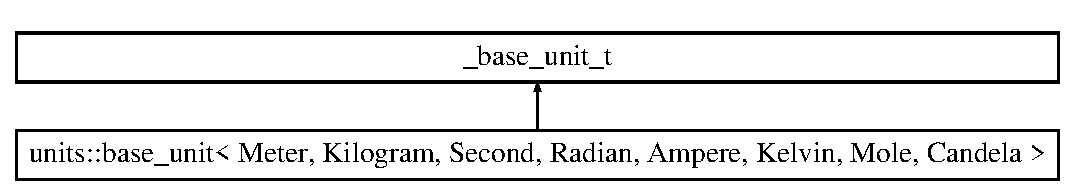
\includegraphics[height=2.000000cm]{structunits_1_1base__unit}
\end{center}
\end{figure}


\subsection{Detailed Description}
\subsubsection*{template$<$class Meter = std\+::ratio$<$0$>$, class Kilogram = std\+::ratio$<$0$>$, class Second = std\+::ratio$<$0$>$, class Radian = std\+::ratio$<$0$>$, class Ampere = std\+::ratio$<$0$>$, class Kelvin = std\+::ratio$<$0$>$, class Mole = std\+::ratio$<$0$>$, class Candela = std\+::ratio $<$ 0 $>$$>$struct units\+::base\+\_\+unit$<$ Meter, Kilogram, Second, Radian, Ampere, Kelvin, Mole, Candela $>$}

Class representing S\+I base unit types. 

Base units are represented by a combination of {\ttfamily std\+::ratio} template parameters, each describing the exponent of the type of unit they represent. Example\+: meters per second would be described by a +1 exponent for meters, and a -\/1 exponent for seconds, thus\+: {\ttfamily \hyperlink{structunits_1_1base__unit}{base\+\_\+unit}$<$std\+::ratio$<$1$>$, std\+::ratio$<$0$>$, std\+::ratio$<$-\/1$>$$>$} 
\begin{DoxyTemplParams}{Template Parameters}
{\em Meter} & {\ttfamily std\+::ratio} representing the exponent value for meters. \\
\hline
{\em Kilogram} & {\ttfamily std\+::ratio} representing the exponent value for kilograms. \\
\hline
{\em Second} & {\ttfamily std\+::ratio} representing the exponent value for seconds. \\
\hline
{\em Radian} & {\ttfamily std\+::ratio} representing the exponent value for radians. Although radians are not S\+I base units, they are included because radians are described by the S\+I as m $\ast$ m$^\wedge$-\/1, which would make them indistinguishable from scalars. \\
\hline
{\em Ampere} & {\ttfamily std\+::ratio} representing the exponent value for amperes. \\
\hline
{\em Kelvin} & {\ttfamily std\+::ratio} representing the exponent value for Kelvin. \\
\hline
{\em Mole} & {\ttfamily std\+::ratio} representing the exponent value for moles. \\
\hline
{\em Candela} & {\ttfamily std\+::ratio} representing the exponent value for candelas. \\
\hline
\end{DoxyTemplParams}
\begin{DoxySeeAlso}{See also}
\hyperlink{namespaceunits_1_1category}{category} for type aliases for S\+I \hyperlink{structunits_1_1base__unit}{base\+\_\+unit} types. 
\end{DoxySeeAlso}


The documentation for this struct was generated from the following file\+:\begin{DoxyCompactItemize}
\item 
/home/nholthaus/workspace/units/include/\hyperlink{units_8h}{units.\+h}\end{DoxyCompactItemize}

\hypertarget{structunits_1_1decibel__scale}{}\section{units\+:\+:decibel\+\_\+scale$<$ T $>$ Struct Template Reference}
\label{structunits_1_1decibel__scale}\index{units\+::decibel\+\_\+scale$<$ T $>$@{units\+::decibel\+\_\+scale$<$ T $>$}}


\hyperlink{classunits_1_1unit__t}{unit\+\_\+t} scale for representing decibel values.  




{\ttfamily \#include $<$units.\+h$>$}

\subsection*{Public Member Functions}
\begin{DoxyCompactItemize}
\item 
\hypertarget{structunits_1_1decibel__scale_a4a7ed3c7b2fce24663ea575d96105991}{}{\bfseries decibel\+\_\+scale} (T value)\label{structunits_1_1decibel__scale_a4a7ed3c7b2fce24663ea575d96105991}

\item 
\hypertarget{structunits_1_1decibel__scale_a533c8316c4ae1839f00822bc1e7bf715}{}T {\bfseries operator()} () const \label{structunits_1_1decibel__scale_a533c8316c4ae1839f00822bc1e7bf715}

\end{DoxyCompactItemize}
\subsection*{Public Attributes}
\begin{DoxyCompactItemize}
\item 
\hypertarget{structunits_1_1decibel__scale_a9716193561ed712aeafdd6b86e376936}{}T \hyperlink{structunits_1_1decibel__scale_a9716193561ed712aeafdd6b86e376936}{m\+\_\+value}\label{structunits_1_1decibel__scale_a9716193561ed712aeafdd6b86e376936}

\begin{DoxyCompactList}\small\item\em linearized value \end{DoxyCompactList}\end{DoxyCompactItemize}


\subsection{Detailed Description}
\subsubsection*{template$<$typename T$>$struct units\+::decibel\+\_\+scale$<$ T $>$}

\hyperlink{classunits_1_1unit__t}{unit\+\_\+t} scale for representing decibel values. 

internally stores linearized values. {\ttfamily operator()} returns the value in d\+B. 
\begin{DoxyTemplParams}{Template Parameters}
{\em T} & underlying storage type \\
\hline
\end{DoxyTemplParams}
\begin{DoxySeeAlso}{See also}
\hyperlink{classunits_1_1unit__t}{unit\+\_\+t} 
\end{DoxySeeAlso}


The documentation for this struct was generated from the following file\+:\begin{DoxyCompactItemize}
\item 
/home/nholthaus/workspace/units/include/\hyperlink{units_8h}{units.\+h}\end{DoxyCompactItemize}

\hypertarget{structunits_1_1traits_1_1has__decibel__scale}{}\section{units\+:\+:traits\+:\+:has\+\_\+decibel\+\_\+scale$<$ T $>$ Struct Template Reference}
\label{structunits_1_1traits_1_1has__decibel__scale}\index{units\+::traits\+::has\+\_\+decibel\+\_\+scale$<$ T $>$@{units\+::traits\+::has\+\_\+decibel\+\_\+scale$<$ T $>$}}


Trait which tests whether a type is inherited from a decibel scale.  




{\ttfamily \#include $<$units.\+h$>$}

Inheritance diagram for units\+:\+:traits\+:\+:has\+\_\+decibel\+\_\+scale$<$ T $>$\+:\begin{figure}[H]
\begin{center}
\leavevmode
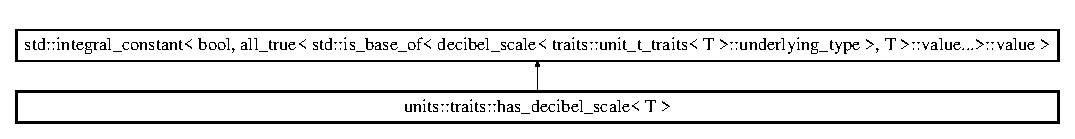
\includegraphics[height=1.414141cm]{structunits_1_1traits_1_1has__decibel__scale}
\end{center}
\end{figure}


\subsection{Detailed Description}
\subsubsection*{template$<$typename... T$>$struct units\+::traits\+::has\+\_\+decibel\+\_\+scale$<$ T $>$}

Trait which tests whether a type is inherited from a decibel scale. 

Inherits from {\ttfamily std\+::true\+\_\+type} or {\ttfamily std\+::false\+\_\+type}. Use {\ttfamily \hyperlink{structunits_1_1traits_1_1has__decibel__scale}{has\+\_\+decibel\+\_\+scale}$<$U1 \mbox{[}, U2, ...\mbox{]}$>$\+::value} to test one or more types to see if they represent \hyperlink{classunits_1_1unit__t}{unit\+\_\+t}\textquotesingle{}s whose scale is in decibels. 
\begin{DoxyTemplParams}{Template Parameters}
{\em T} & one or more types to test. \\
\hline
\end{DoxyTemplParams}


The documentation for this struct was generated from the following file\+:\begin{DoxyCompactItemize}
\item 
/home/nholthaus/workspace/units/include/\hyperlink{units_8h}{units.\+h}\end{DoxyCompactItemize}

\hypertarget{structunits_1_1traits_1_1has__linear__scale}{}\section{units\+:\+:traits\+:\+:has\+\_\+linear\+\_\+scale$<$ T $>$ Struct Template Reference}
\label{structunits_1_1traits_1_1has__linear__scale}\index{units\+::traits\+::has\+\_\+linear\+\_\+scale$<$ T $>$@{units\+::traits\+::has\+\_\+linear\+\_\+scale$<$ T $>$}}


Trait which tests whether a type is inherited from a linear scale.  




{\ttfamily \#include $<$units.\+h$>$}

Inheritance diagram for units\+:\+:traits\+:\+:has\+\_\+linear\+\_\+scale$<$ T $>$\+:\begin{figure}[H]
\begin{center}
\leavevmode
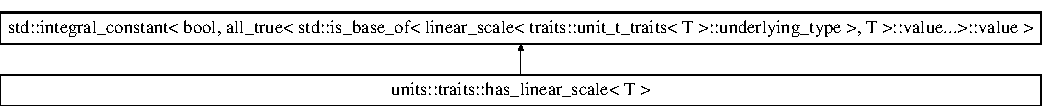
\includegraphics[height=1.430396cm]{structunits_1_1traits_1_1has__linear__scale}
\end{center}
\end{figure}


\subsection{Detailed Description}
\subsubsection*{template$<$typename... T$>$struct units\+::traits\+::has\+\_\+linear\+\_\+scale$<$ T $>$}

Trait which tests whether a type is inherited from a linear scale. 

Inherits from {\ttfamily std\+::true\+\_\+type} or {\ttfamily std\+::false\+\_\+type}. Use {\ttfamily \hyperlink{structunits_1_1traits_1_1has__linear__scale}{has\+\_\+linear\+\_\+scale}$<$U1 \mbox{[}, U2, ...\mbox{]}$>$\+::value} to test one or more types to see if they represent \hyperlink{classunits_1_1unit__t}{unit\+\_\+t}\textquotesingle{}s whose scale is linear. 
\begin{DoxyTemplParams}{Template Parameters}
{\em T} & one or more types to test. \\
\hline
\end{DoxyTemplParams}


The documentation for this struct was generated from the following file\+:\begin{DoxyCompactItemize}
\item 
/home/nholthaus/workspace/units/include/\hyperlink{units_8h}{units.\+h}\end{DoxyCompactItemize}

\hypertarget{structunits_1_1traits_1_1is__acceleration__unit}{}\section{units\+:\+:traits\+:\+:is\+\_\+acceleration\+\_\+unit$<$ T $>$ Struct Template Reference}
\label{structunits_1_1traits_1_1is__acceleration__unit}\index{units\+::traits\+::is\+\_\+acceleration\+\_\+unit$<$ T $>$@{units\+::traits\+::is\+\_\+acceleration\+\_\+unit$<$ T $>$}}


Trait which tests whether a type represents a unit of acceleration.  




{\ttfamily \#include $<$units.\+h$>$}

Inheritance diagram for units\+:\+:traits\+:\+:is\+\_\+acceleration\+\_\+unit$<$ T $>$\+:\begin{figure}[H]
\begin{center}
\leavevmode
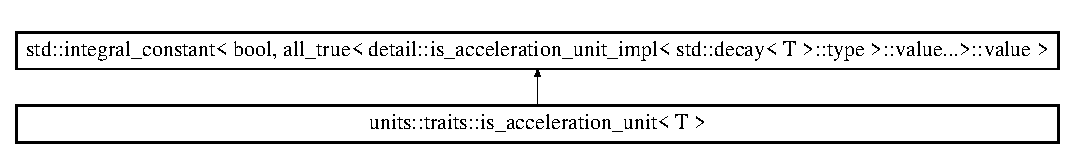
\includegraphics[height=1.691843cm]{structunits_1_1traits_1_1is__acceleration__unit}
\end{center}
\end{figure}


\subsection{Detailed Description}
\subsubsection*{template$<$typename... T$>$struct units\+::traits\+::is\+\_\+acceleration\+\_\+unit$<$ T $>$}

Trait which tests whether a type represents a unit of acceleration. 

Inherits from {\ttfamily std\+::true\+\_\+type} or {\ttfamily std\+::false\+\_\+type}. Use {\ttfamily \hyperlink{structunits_1_1traits_1_1is__acceleration__unit}{is\+\_\+acceleration\+\_\+unit}$<$T$>$\+::value} to test the unit represents a acceleration quantity. 
\begin{DoxyTemplParams}{Template Parameters}
{\em T} & one or more types to test \\
\hline
\end{DoxyTemplParams}


The documentation for this struct was generated from the following file\+:\begin{DoxyCompactItemize}
\item 
/home/nholthaus/workspace/units/include/\hyperlink{units_8h}{units.\+h}\end{DoxyCompactItemize}

\hypertarget{structunits_1_1traits_1_1is__angle__unit}{}\section{units\+:\+:traits\+:\+:is\+\_\+angle\+\_\+unit$<$ T $>$ Struct Template Reference}
\label{structunits_1_1traits_1_1is__angle__unit}\index{units\+::traits\+::is\+\_\+angle\+\_\+unit$<$ T $>$@{units\+::traits\+::is\+\_\+angle\+\_\+unit$<$ T $>$}}


Trait which tests whether a type represents a unit of angle.  




{\ttfamily \#include $<$units.\+h$>$}

Inheritance diagram for units\+:\+:traits\+:\+:is\+\_\+angle\+\_\+unit$<$ T $>$\+:\begin{figure}[H]
\begin{center}
\leavevmode
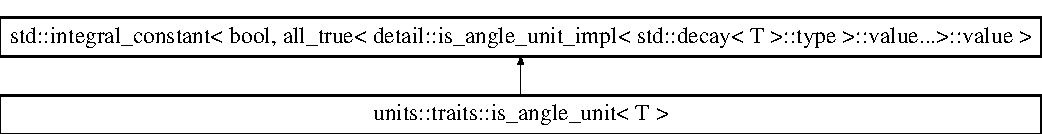
\includegraphics[height=1.797753cm]{structunits_1_1traits_1_1is__angle__unit}
\end{center}
\end{figure}


\subsection{Detailed Description}
\subsubsection*{template$<$typename... T$>$struct units\+::traits\+::is\+\_\+angle\+\_\+unit$<$ T $>$}

Trait which tests whether a type represents a unit of angle. 

Inherits from {\ttfamily std\+::true\+\_\+type} or {\ttfamily std\+::false\+\_\+type}. Use {\ttfamily \hyperlink{structunits_1_1traits_1_1is__angle__unit}{is\+\_\+angle\+\_\+unit}$<$T$>$\+::value} to test the unit represents a angle quantity. 
\begin{DoxyTemplParams}{Template Parameters}
{\em T} & one or more types to test \\
\hline
\end{DoxyTemplParams}


The documentation for this struct was generated from the following file\+:\begin{DoxyCompactItemize}
\item 
/home/nholthaus/workspace/units/include/\hyperlink{units_8h}{units.\+h}\end{DoxyCompactItemize}

\hypertarget{structunits_1_1traits_1_1is__angular__velocity__unit}{}\section{units\+:\+:traits\+:\+:is\+\_\+angular\+\_\+velocity\+\_\+unit$<$ T $>$ Struct Template Reference}
\label{structunits_1_1traits_1_1is__angular__velocity__unit}\index{units\+::traits\+::is\+\_\+angular\+\_\+velocity\+\_\+unit$<$ T $>$@{units\+::traits\+::is\+\_\+angular\+\_\+velocity\+\_\+unit$<$ T $>$}}


Trait which tests whether a type represents a unit of \hyperlink{namespaceunits_1_1angular__velocity}{angular\+\_\+velocity}.  




{\ttfamily \#include $<$units.\+h$>$}

Inheritance diagram for units\+:\+:traits\+:\+:is\+\_\+angular\+\_\+velocity\+\_\+unit$<$ T $>$\+:\begin{figure}[H]
\begin{center}
\leavevmode
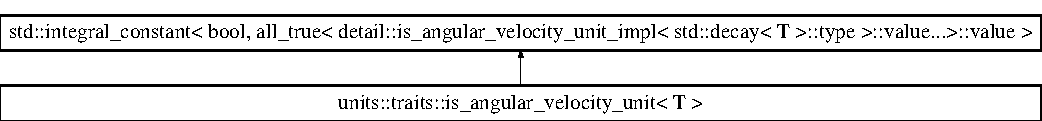
\includegraphics[height=1.632653cm]{structunits_1_1traits_1_1is__angular__velocity__unit}
\end{center}
\end{figure}


\subsection{Detailed Description}
\subsubsection*{template$<$typename... T$>$struct units\+::traits\+::is\+\_\+angular\+\_\+velocity\+\_\+unit$<$ T $>$}

Trait which tests whether a type represents a unit of \hyperlink{namespaceunits_1_1angular__velocity}{angular\+\_\+velocity}. 

Inherits from {\ttfamily std\+::true\+\_\+type} or {\ttfamily std\+::false\+\_\+type}. Use {\ttfamily \hyperlink{structunits_1_1traits_1_1is__angular__velocity__unit}{is\+\_\+angular\+\_\+velocity\+\_\+unit}$<$T$>$\+::value} to test the unit represents a \hyperlink{namespaceunits_1_1angular__velocity}{angular\+\_\+velocity} quantity. 
\begin{DoxyTemplParams}{Template Parameters}
{\em T} & one or more types to test \\
\hline
\end{DoxyTemplParams}


The documentation for this struct was generated from the following file\+:\begin{DoxyCompactItemize}
\item 
/home/nholthaus/workspace/units/include/\hyperlink{units_8h}{units.\+h}\end{DoxyCompactItemize}

\hypertarget{structunits_1_1traits_1_1is__area__unit}{}\section{units\+:\+:traits\+:\+:is\+\_\+area\+\_\+unit$<$ T $>$ Struct Template Reference}
\label{structunits_1_1traits_1_1is__area__unit}\index{units\+::traits\+::is\+\_\+area\+\_\+unit$<$ T $>$@{units\+::traits\+::is\+\_\+area\+\_\+unit$<$ T $>$}}


Trait which tests whether a type represents a unit of area.  




{\ttfamily \#include $<$units.\+h$>$}

Inheritance diagram for units\+:\+:traits\+:\+:is\+\_\+area\+\_\+unit$<$ T $>$\+:\begin{figure}[H]
\begin{center}
\leavevmode
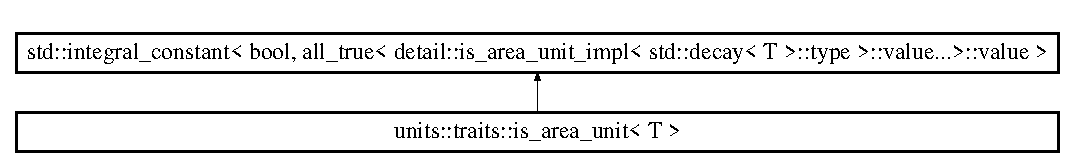
\includegraphics[height=1.812298cm]{structunits_1_1traits_1_1is__area__unit}
\end{center}
\end{figure}


\subsection{Detailed Description}
\subsubsection*{template$<$typename... T$>$struct units\+::traits\+::is\+\_\+area\+\_\+unit$<$ T $>$}

Trait which tests whether a type represents a unit of area. 

Inherits from {\ttfamily std\+::true\+\_\+type} or {\ttfamily std\+::false\+\_\+type}. Use {\ttfamily \hyperlink{structunits_1_1traits_1_1is__area__unit}{is\+\_\+area\+\_\+unit}$<$T$>$\+::value} to test the unit represents a area quantity. 
\begin{DoxyTemplParams}{Template Parameters}
{\em T} & one or more types to test \\
\hline
\end{DoxyTemplParams}


The documentation for this struct was generated from the following file\+:\begin{DoxyCompactItemize}
\item 
/home/nholthaus/workspace/units/include/\hyperlink{units_8h}{units.\+h}\end{DoxyCompactItemize}

\hypertarget{structunits_1_1traits_1_1is__base__unit}{}\section{units\+:\+:traits\+:\+:is\+\_\+base\+\_\+unit$<$ T $>$ Struct Template Reference}
\label{structunits_1_1traits_1_1is__base__unit}\index{units\+::traits\+::is\+\_\+base\+\_\+unit$<$ T $>$@{units\+::traits\+::is\+\_\+base\+\_\+unit$<$ T $>$}}


Trait which tests if a class is a {\ttfamily \hyperlink{structunits_1_1base__unit}{base\+\_\+unit}} type.  




{\ttfamily \#include $<$units.\+h$>$}

Inheritance diagram for units\+:\+:traits\+:\+:is\+\_\+base\+\_\+unit$<$ T $>$\+:\begin{figure}[H]
\begin{center}
\leavevmode
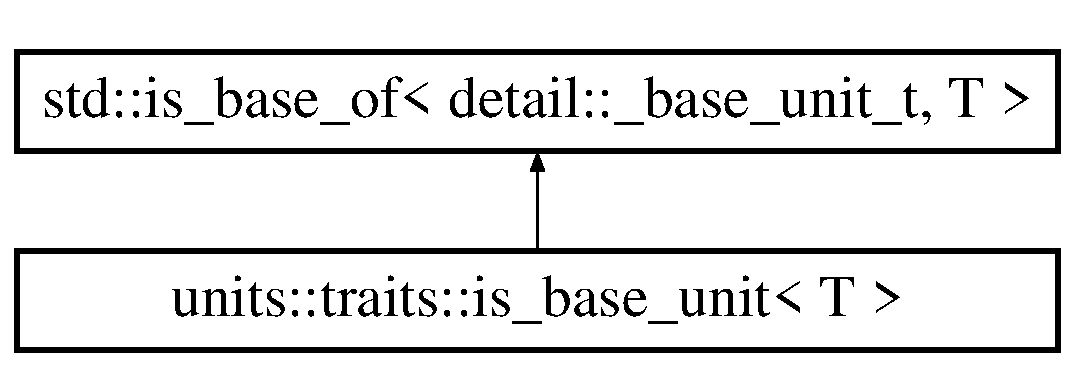
\includegraphics[height=2.000000cm]{structunits_1_1traits_1_1is__base__unit}
\end{center}
\end{figure}


\subsection{Detailed Description}
\subsubsection*{template$<$class T$>$struct units\+::traits\+::is\+\_\+base\+\_\+unit$<$ T $>$}

Trait which tests if a class is a {\ttfamily \hyperlink{structunits_1_1base__unit}{base\+\_\+unit}} type. 

Inherits from {\ttfamily std\+::true\+\_\+type} or {\ttfamily std\+::false\+\_\+type}. Use {\ttfamily \hyperlink{structunits_1_1traits_1_1is__base__unit}{is\+\_\+base\+\_\+unit}$<$T$>$\+::value} to test whether {\ttfamily class T} implements a {\ttfamily \hyperlink{structunits_1_1base__unit}{base\+\_\+unit}}. 

The documentation for this struct was generated from the following file\+:\begin{DoxyCompactItemize}
\item 
/home/nholthaus/workspace/units/include/\hyperlink{units_8h}{units.\+h}\end{DoxyCompactItemize}

\hypertarget{structunits_1_1traits_1_1is__capacitance__unit}{}\section{units\+:\+:traits\+:\+:is\+\_\+capacitance\+\_\+unit$<$ T $>$ Struct Template Reference}
\label{structunits_1_1traits_1_1is__capacitance__unit}\index{units\+::traits\+::is\+\_\+capacitance\+\_\+unit$<$ T $>$@{units\+::traits\+::is\+\_\+capacitance\+\_\+unit$<$ T $>$}}


Trait which tests whether a type represents a unit of capacitance.  




{\ttfamily \#include $<$units.\+h$>$}

Inheritance diagram for units\+:\+:traits\+:\+:is\+\_\+capacitance\+\_\+unit$<$ T $>$\+:\begin{figure}[H]
\begin{center}
\leavevmode
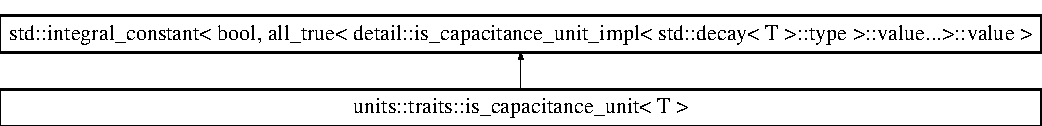
\includegraphics[height=1.694402cm]{structunits_1_1traits_1_1is__capacitance__unit}
\end{center}
\end{figure}


\subsection{Detailed Description}
\subsubsection*{template$<$typename... T$>$struct units\+::traits\+::is\+\_\+capacitance\+\_\+unit$<$ T $>$}

Trait which tests whether a type represents a unit of capacitance. 

Inherits from {\ttfamily std\+::true\+\_\+type} or {\ttfamily std\+::false\+\_\+type}. Use {\ttfamily \hyperlink{structunits_1_1traits_1_1is__capacitance__unit}{is\+\_\+capacitance\+\_\+unit}$<$T$>$\+::value} to test the unit represents a capacitance quantity. 
\begin{DoxyTemplParams}{Template Parameters}
{\em T} & one or more types to test \\
\hline
\end{DoxyTemplParams}


The documentation for this struct was generated from the following file\+:\begin{DoxyCompactItemize}
\item 
/home/nholthaus/workspace/units/include/\hyperlink{units_8h}{units.\+h}\end{DoxyCompactItemize}

\hypertarget{structunits_1_1traits_1_1is__charge__unit}{}\section{units\+:\+:traits\+:\+:is\+\_\+charge\+\_\+unit$<$ T $>$ Struct Template Reference}
\label{structunits_1_1traits_1_1is__charge__unit}\index{units\+::traits\+::is\+\_\+charge\+\_\+unit$<$ T $>$@{units\+::traits\+::is\+\_\+charge\+\_\+unit$<$ T $>$}}


Trait which tests whether a type represents a unit of charge.  




{\ttfamily \#include $<$units.\+h$>$}

Inheritance diagram for units\+:\+:traits\+:\+:is\+\_\+charge\+\_\+unit$<$ T $>$\+:\begin{figure}[H]
\begin{center}
\leavevmode
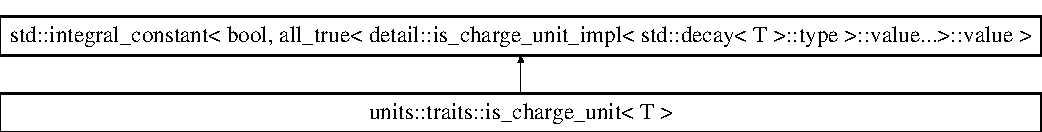
\includegraphics[height=1.772152cm]{structunits_1_1traits_1_1is__charge__unit}
\end{center}
\end{figure}


\subsection{Detailed Description}
\subsubsection*{template$<$typename... T$>$struct units\+::traits\+::is\+\_\+charge\+\_\+unit$<$ T $>$}

Trait which tests whether a type represents a unit of charge. 

Inherits from {\ttfamily std\+::true\+\_\+type} or {\ttfamily std\+::false\+\_\+type}. Use {\ttfamily \hyperlink{structunits_1_1traits_1_1is__charge__unit}{is\+\_\+charge\+\_\+unit}$<$T$>$\+::value} to test the unit represents a charge quantity. 
\begin{DoxyTemplParams}{Template Parameters}
{\em T} & one or more types to test \\
\hline
\end{DoxyTemplParams}


The documentation for this struct was generated from the following file\+:\begin{DoxyCompactItemize}
\item 
/home/nholthaus/workspace/units/include/\hyperlink{units_8h}{units.\+h}\end{DoxyCompactItemize}

\hypertarget{structunits_1_1traits_1_1is__concentration__unit}{}\section{units\+:\+:traits\+:\+:is\+\_\+concentration\+\_\+unit$<$ T $>$ Struct Template Reference}
\label{structunits_1_1traits_1_1is__concentration__unit}\index{units\+::traits\+::is\+\_\+concentration\+\_\+unit$<$ T $>$@{units\+::traits\+::is\+\_\+concentration\+\_\+unit$<$ T $>$}}


Trait which tests whether a type represents a unit of concentration.  




{\ttfamily \#include $<$units.\+h$>$}

Inheritance diagram for units\+:\+:traits\+:\+:is\+\_\+concentration\+\_\+unit$<$ T $>$\+:\begin{figure}[H]
\begin{center}
\leavevmode
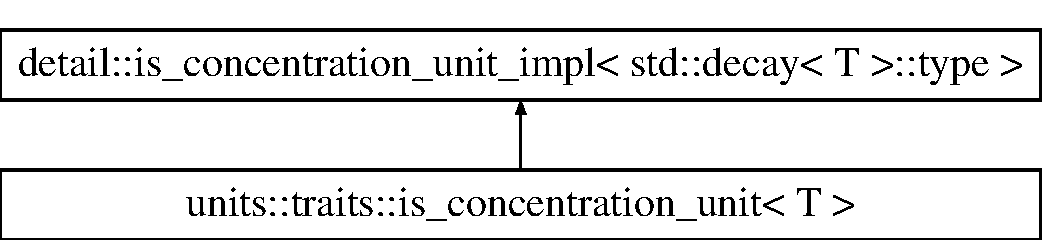
\includegraphics[height=2.000000cm]{structunits_1_1traits_1_1is__concentration__unit}
\end{center}
\end{figure}


\subsection{Detailed Description}
\subsubsection*{template$<$typename T$>$struct units\+::traits\+::is\+\_\+concentration\+\_\+unit$<$ T $>$}

Trait which tests whether a type represents a unit of concentration. 

Inherits from {\ttfamily std\+::true\+\_\+type} or {\ttfamily std\+::false\+\_\+type}. Use {\ttfamily \hyperlink{structunits_1_1traits_1_1is__concentration__unit}{is\+\_\+concentration\+\_\+unit}$<$T$>$\+::value} to test the unit represents a concentration quantity. 
\begin{DoxyTemplParams}{Template Parameters}
{\em T} & one or more types to test \\
\hline
\end{DoxyTemplParams}


The documentation for this struct was generated from the following file\+:\begin{DoxyCompactItemize}
\item 
/home/nholthaus/workspace/units/include/\hyperlink{units_8h}{units.\+h}\end{DoxyCompactItemize}

\hypertarget{structunits_1_1traits_1_1is__conductance__unit}{}\section{units\+:\+:traits\+:\+:is\+\_\+conductance\+\_\+unit$<$ T $>$ Struct Template Reference}
\label{structunits_1_1traits_1_1is__conductance__unit}\index{units\+::traits\+::is\+\_\+conductance\+\_\+unit$<$ T $>$@{units\+::traits\+::is\+\_\+conductance\+\_\+unit$<$ T $>$}}


Trait which tests whether a type represents a unit of conductance.  




{\ttfamily \#include $<$units.\+h$>$}

Inheritance diagram for units\+:\+:traits\+:\+:is\+\_\+conductance\+\_\+unit$<$ T $>$\+:\begin{figure}[H]
\begin{center}
\leavevmode
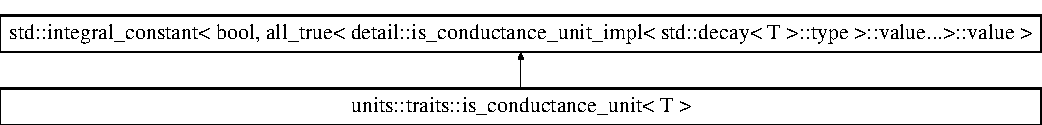
\includegraphics[height=1.684211cm]{structunits_1_1traits_1_1is__conductance__unit}
\end{center}
\end{figure}


\subsection{Detailed Description}
\subsubsection*{template$<$typename... T$>$struct units\+::traits\+::is\+\_\+conductance\+\_\+unit$<$ T $>$}

Trait which tests whether a type represents a unit of conductance. 

Inherits from {\ttfamily std\+::true\+\_\+type} or {\ttfamily std\+::false\+\_\+type}. Use {\ttfamily \hyperlink{structunits_1_1traits_1_1is__conductance__unit}{is\+\_\+conductance\+\_\+unit}$<$T$>$\+::value} to test the unit represents a conductance quantity. 
\begin{DoxyTemplParams}{Template Parameters}
{\em T} & one or more types to test \\
\hline
\end{DoxyTemplParams}


The documentation for this struct was generated from the following file\+:\begin{DoxyCompactItemize}
\item 
/home/nholthaus/workspace/units/include/\hyperlink{units_8h}{units.\+h}\end{DoxyCompactItemize}

\hypertarget{structunits_1_1traits_1_1is__convertible__unit}{}\section{units\+:\+:traits\+:\+:is\+\_\+convertible\+\_\+unit$<$ U1, U2 $>$ Struct Template Reference}
\label{structunits_1_1traits_1_1is__convertible__unit}\index{units\+::traits\+::is\+\_\+convertible\+\_\+unit$<$ U1, U2 $>$@{units\+::traits\+::is\+\_\+convertible\+\_\+unit$<$ U1, U2 $>$}}


Trait which checks whether two units can be converted to each other.  




{\ttfamily \#include $<$units.\+h$>$}

Inheritance diagram for units\+:\+:traits\+:\+:is\+\_\+convertible\+\_\+unit$<$ U1, U2 $>$\+:\begin{figure}[H]
\begin{center}
\leavevmode
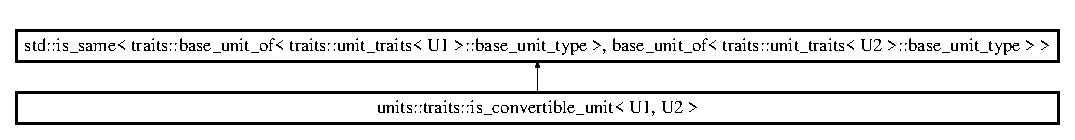
\includegraphics[height=1.437741cm]{structunits_1_1traits_1_1is__convertible__unit}
\end{center}
\end{figure}


\subsection{Detailed Description}
\subsubsection*{template$<$class U1, class U2$>$struct units\+::traits\+::is\+\_\+convertible\+\_\+unit$<$ U1, U2 $>$}

Trait which checks whether two units can be converted to each other. 

Inherits from {\ttfamily std\+::true\+\_\+type} or {\ttfamily std\+::false\+\_\+type}. Use {\ttfamily \hyperlink{structunits_1_1traits_1_1is__convertible__unit}{is\+\_\+convertible\+\_\+unit}$<$U1, U2$>$\+::value} to test whether {\ttfamily class U1} is convertible to {\ttfamily class U2}. Note\+: convertible has both the semantic meaning, (i.\+e. meters can be converted to feet), and the c++ meaning of conversion (type meters can be converted to type feet). Conversion is always symmetric, so if U1 is convertible to U2, then U2 will be convertible to U1. 
\begin{DoxyTemplParams}{Template Parameters}
{\em U1} & Unit to convert from. \\
\hline
{\em U2} & Unit to convert to. \\
\hline
\end{DoxyTemplParams}
\begin{DoxySeeAlso}{See also}
\hyperlink{structunits_1_1traits_1_1is__convertible__unit__t}{is\+\_\+convertible\+\_\+unit\+\_\+t} 
\end{DoxySeeAlso}


The documentation for this struct was generated from the following file\+:\begin{DoxyCompactItemize}
\item 
/home/nholthaus/workspace/units/include/\hyperlink{units_8h}{units.\+h}\end{DoxyCompactItemize}

\hypertarget{structunits_1_1traits_1_1is__convertible__unit__t}{}\section{units\+:\+:traits\+:\+:is\+\_\+convertible\+\_\+unit\+\_\+t$<$ U1, U2 $>$ Struct Template Reference}
\label{structunits_1_1traits_1_1is__convertible__unit__t}\index{units\+::traits\+::is\+\_\+convertible\+\_\+unit\+\_\+t$<$ U1, U2 $>$@{units\+::traits\+::is\+\_\+convertible\+\_\+unit\+\_\+t$<$ U1, U2 $>$}}


Trait which tests whether two container types derived from {\ttfamily \hyperlink{classunits_1_1unit__t}{unit\+\_\+t}} are convertible to each other.  




{\ttfamily \#include $<$units.\+h$>$}

Inheritance diagram for units\+:\+:traits\+:\+:is\+\_\+convertible\+\_\+unit\+\_\+t$<$ U1, U2 $>$\+:\begin{figure}[H]
\begin{center}
\leavevmode
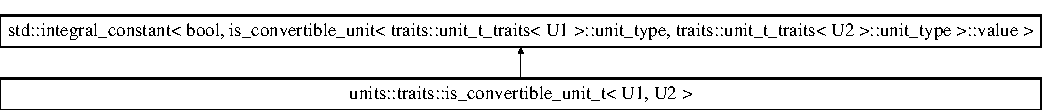
\includegraphics[height=1.479524cm]{structunits_1_1traits_1_1is__convertible__unit__t}
\end{center}
\end{figure}


\subsection{Detailed Description}
\subsubsection*{template$<$class U1, class U2$>$struct units\+::traits\+::is\+\_\+convertible\+\_\+unit\+\_\+t$<$ U1, U2 $>$}

Trait which tests whether two container types derived from {\ttfamily \hyperlink{classunits_1_1unit__t}{unit\+\_\+t}} are convertible to each other. 

Inherits from {\ttfamily std\+::true\+\_\+type} or {\ttfamily std\+::false\+\_\+type}. Use {\ttfamily \hyperlink{structunits_1_1traits_1_1is__convertible__unit__t}{is\+\_\+convertible\+\_\+unit\+\_\+t}$<$U1, U2$>$\+::value} to test whether {\ttfamily class U1} is convertible to {\ttfamily class U2}. Note\+: convertible has both the semantic meaning, (i.\+e. meters can be converted to feet), and the c++ meaning of conversion (type meters can be converted to type feet). Conversion is always symmetric, so if U1 is convertible to U2, then U2 will be convertible to U1. 
\begin{DoxyTemplParams}{Template Parameters}
{\em U1} & Unit to convert from. \\
\hline
{\em U2} & Unit to convert to. \\
\hline
\end{DoxyTemplParams}
\begin{DoxySeeAlso}{See also}
\hyperlink{structunits_1_1traits_1_1is__convertible__unit}{is\+\_\+convertible\+\_\+unit} 
\end{DoxySeeAlso}


The documentation for this struct was generated from the following file\+:\begin{DoxyCompactItemize}
\item 
/home/nholthaus/workspace/units/include/\hyperlink{units_8h}{units.\+h}\end{DoxyCompactItemize}

\hypertarget{structunits_1_1traits_1_1is__current__unit}{}\section{units\+:\+:traits\+:\+:is\+\_\+current\+\_\+unit$<$ T $>$ Struct Template Reference}
\label{structunits_1_1traits_1_1is__current__unit}\index{units\+::traits\+::is\+\_\+current\+\_\+unit$<$ T $>$@{units\+::traits\+::is\+\_\+current\+\_\+unit$<$ T $>$}}


Trait which tests whether a type represents a unit of current.  




{\ttfamily \#include $<$units.\+h$>$}

Inheritance diagram for units\+:\+:traits\+:\+:is\+\_\+current\+\_\+unit$<$ T $>$\+:\begin{figure}[H]
\begin{center}
\leavevmode
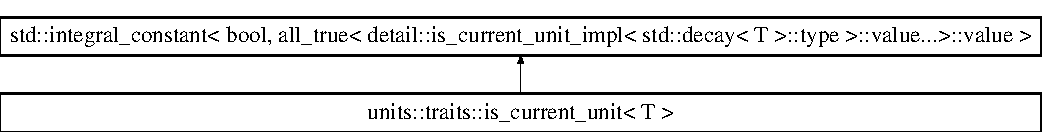
\includegraphics[height=1.769352cm]{structunits_1_1traits_1_1is__current__unit}
\end{center}
\end{figure}


\subsection{Detailed Description}
\subsubsection*{template$<$typename... T$>$struct units\+::traits\+::is\+\_\+current\+\_\+unit$<$ T $>$}

Trait which tests whether a type represents a unit of current. 

Inherits from {\ttfamily std\+::true\+\_\+type} or {\ttfamily std\+::false\+\_\+type}. Use {\ttfamily \hyperlink{structunits_1_1traits_1_1is__current__unit}{is\+\_\+current\+\_\+unit}$<$T$>$\+::value} to test the unit represents a current quantity. 
\begin{DoxyTemplParams}{Template Parameters}
{\em T} & one or more types to test \\
\hline
\end{DoxyTemplParams}


The documentation for this struct was generated from the following file\+:\begin{DoxyCompactItemize}
\item 
/home/nholthaus/workspace/units/include/\hyperlink{units_8h}{units.\+h}\end{DoxyCompactItemize}

\hypertarget{structunits_1_1traits_1_1is__density__unit}{}\section{units\+:\+:traits\+:\+:is\+\_\+density\+\_\+unit$<$ T $>$ Struct Template Reference}
\label{structunits_1_1traits_1_1is__density__unit}\index{units\+::traits\+::is\+\_\+density\+\_\+unit$<$ T $>$@{units\+::traits\+::is\+\_\+density\+\_\+unit$<$ T $>$}}


Trait which tests whether a type represents a unit of density.  




{\ttfamily \#include $<$units.\+h$>$}

Inheritance diagram for units\+:\+:traits\+:\+:is\+\_\+density\+\_\+unit$<$ T $>$\+:\begin{figure}[H]
\begin{center}
\leavevmode
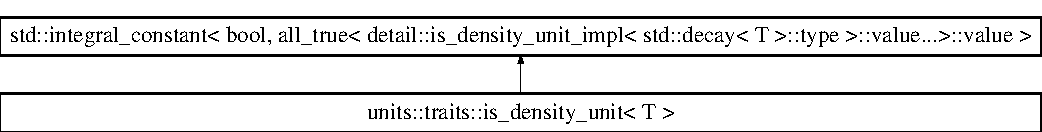
\includegraphics[height=1.772152cm]{structunits_1_1traits_1_1is__density__unit}
\end{center}
\end{figure}


\subsection{Detailed Description}
\subsubsection*{template$<$typename... T$>$struct units\+::traits\+::is\+\_\+density\+\_\+unit$<$ T $>$}

Trait which tests whether a type represents a unit of density. 

Inherits from {\ttfamily std\+::true\+\_\+type} or {\ttfamily std\+::false\+\_\+type}. Use {\ttfamily \hyperlink{structunits_1_1traits_1_1is__density__unit}{is\+\_\+density\+\_\+unit}$<$T$>$\+::value} to test the unit represents a density quantity. 
\begin{DoxyTemplParams}{Template Parameters}
{\em T} & one or more types to test \\
\hline
\end{DoxyTemplParams}


The documentation for this struct was generated from the following file\+:\begin{DoxyCompactItemize}
\item 
/home/nholthaus/workspace/units/include/\hyperlink{units_8h}{units.\+h}\end{DoxyCompactItemize}

\hypertarget{structunits_1_1traits_1_1is__energy__unit}{}\section{units\+:\+:traits\+:\+:is\+\_\+energy\+\_\+unit$<$ T $>$ Struct Template Reference}
\label{structunits_1_1traits_1_1is__energy__unit}\index{units\+::traits\+::is\+\_\+energy\+\_\+unit$<$ T $>$@{units\+::traits\+::is\+\_\+energy\+\_\+unit$<$ T $>$}}


Trait which tests whether a type represents a unit of energy.  




{\ttfamily \#include $<$units.\+h$>$}

Inheritance diagram for units\+:\+:traits\+:\+:is\+\_\+energy\+\_\+unit$<$ T $>$\+:\begin{figure}[H]
\begin{center}
\leavevmode
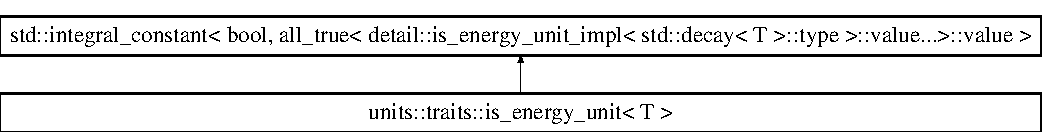
\includegraphics[height=1.772152cm]{structunits_1_1traits_1_1is__energy__unit}
\end{center}
\end{figure}


\subsection{Detailed Description}
\subsubsection*{template$<$typename... T$>$struct units\+::traits\+::is\+\_\+energy\+\_\+unit$<$ T $>$}

Trait which tests whether a type represents a unit of energy. 

Inherits from {\ttfamily std\+::true\+\_\+type} or {\ttfamily std\+::false\+\_\+type}. Use {\ttfamily \hyperlink{structunits_1_1traits_1_1is__energy__unit}{is\+\_\+energy\+\_\+unit}$<$T$>$\+::value} to test the unit represents a energy quantity. 
\begin{DoxyTemplParams}{Template Parameters}
{\em T} & one or more types to test \\
\hline
\end{DoxyTemplParams}


The documentation for this struct was generated from the following file\+:\begin{DoxyCompactItemize}
\item 
/home/nholthaus/workspace/units/include/\hyperlink{units_8h}{units.\+h}\end{DoxyCompactItemize}

\hypertarget{structunits_1_1traits_1_1is__force__unit}{}\section{units\+:\+:traits\+:\+:is\+\_\+force\+\_\+unit$<$ T $>$ Struct Template Reference}
\label{structunits_1_1traits_1_1is__force__unit}\index{units\+::traits\+::is\+\_\+force\+\_\+unit$<$ T $>$@{units\+::traits\+::is\+\_\+force\+\_\+unit$<$ T $>$}}


Trait which tests whether a type represents a unit of force.  




{\ttfamily \#include $<$units.\+h$>$}

Inheritance diagram for units\+:\+:traits\+:\+:is\+\_\+force\+\_\+unit$<$ T $>$\+:\begin{figure}[H]
\begin{center}
\leavevmode
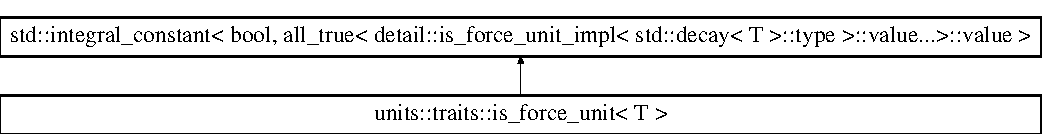
\includegraphics[height=1.800643cm]{structunits_1_1traits_1_1is__force__unit}
\end{center}
\end{figure}


\subsection{Detailed Description}
\subsubsection*{template$<$typename... T$>$struct units\+::traits\+::is\+\_\+force\+\_\+unit$<$ T $>$}

Trait which tests whether a type represents a unit of force. 

Inherits from {\ttfamily std\+::true\+\_\+type} or {\ttfamily std\+::false\+\_\+type}. Use {\ttfamily \hyperlink{structunits_1_1traits_1_1is__force__unit}{is\+\_\+force\+\_\+unit}$<$T$>$\+::value} to test the unit represents a force quantity. 
\begin{DoxyTemplParams}{Template Parameters}
{\em T} & one or more types to test \\
\hline
\end{DoxyTemplParams}


The documentation for this struct was generated from the following file\+:\begin{DoxyCompactItemize}
\item 
/home/nholthaus/workspace/units/include/\hyperlink{units_8h}{units.\+h}\end{DoxyCompactItemize}

\hypertarget{structunits_1_1traits_1_1is__frequency__unit}{}\section{units\+:\+:traits\+:\+:is\+\_\+frequency\+\_\+unit$<$ T $>$ Struct Template Reference}
\label{structunits_1_1traits_1_1is__frequency__unit}\index{units\+::traits\+::is\+\_\+frequency\+\_\+unit$<$ T $>$@{units\+::traits\+::is\+\_\+frequency\+\_\+unit$<$ T $>$}}


Trait which tests whether a type represents a unit of frequency.  




{\ttfamily \#include $<$units.\+h$>$}

Inheritance diagram for units\+:\+:traits\+:\+:is\+\_\+frequency\+\_\+unit$<$ T $>$\+:\begin{figure}[H]
\begin{center}
\leavevmode
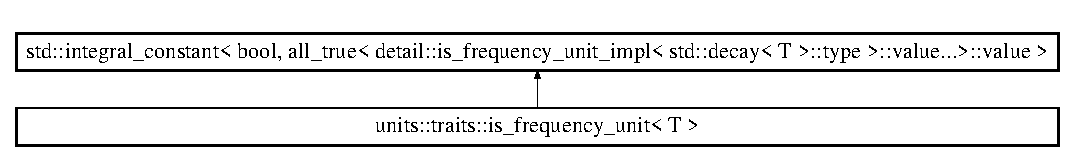
\includegraphics[height=1.725732cm]{structunits_1_1traits_1_1is__frequency__unit}
\end{center}
\end{figure}


\subsection{Detailed Description}
\subsubsection*{template$<$typename... T$>$struct units\+::traits\+::is\+\_\+frequency\+\_\+unit$<$ T $>$}

Trait which tests whether a type represents a unit of frequency. 

Inherits from {\ttfamily std\+::true\+\_\+type} or {\ttfamily std\+::false\+\_\+type}. Use {\ttfamily \hyperlink{structunits_1_1traits_1_1is__frequency__unit}{is\+\_\+frequency\+\_\+unit}$<$T$>$\+::value} to test the unit represents a frequency quantity. 
\begin{DoxyTemplParams}{Template Parameters}
{\em T} & one or more types to test \\
\hline
\end{DoxyTemplParams}


The documentation for this struct was generated from the following file\+:\begin{DoxyCompactItemize}
\item 
/home/nholthaus/workspace/units/include/\hyperlink{units_8h}{units.\+h}\end{DoxyCompactItemize}

\hypertarget{structunits_1_1traits_1_1is__illuminance__unit}{}\section{units\+:\+:traits\+:\+:is\+\_\+illuminance\+\_\+unit$<$ T $>$ Struct Template Reference}
\label{structunits_1_1traits_1_1is__illuminance__unit}\index{units\+::traits\+::is\+\_\+illuminance\+\_\+unit$<$ T $>$@{units\+::traits\+::is\+\_\+illuminance\+\_\+unit$<$ T $>$}}


Trait which tests whether a type represents a unit of illuminance.  




{\ttfamily \#include $<$units.\+h$>$}

Inheritance diagram for units\+:\+:traits\+:\+:is\+\_\+illuminance\+\_\+unit$<$ T $>$\+:\begin{figure}[H]
\begin{center}
\leavevmode
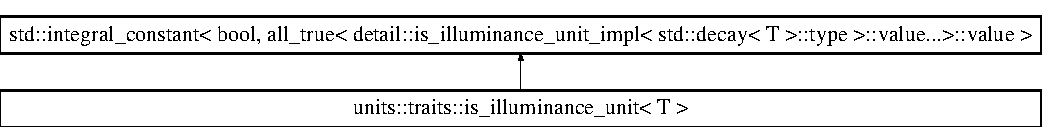
\includegraphics[height=1.709924cm]{structunits_1_1traits_1_1is__illuminance__unit}
\end{center}
\end{figure}


\subsection{Detailed Description}
\subsubsection*{template$<$typename... T$>$struct units\+::traits\+::is\+\_\+illuminance\+\_\+unit$<$ T $>$}

Trait which tests whether a type represents a unit of illuminance. 

Inherits from {\ttfamily std\+::true\+\_\+type} or {\ttfamily std\+::false\+\_\+type}. Use {\ttfamily \hyperlink{structunits_1_1traits_1_1is__illuminance__unit}{is\+\_\+illuminance\+\_\+unit}$<$T$>$\+::value} to test the unit represents a illuminance quantity. 
\begin{DoxyTemplParams}{Template Parameters}
{\em T} & one or more types to test \\
\hline
\end{DoxyTemplParams}


The documentation for this struct was generated from the following file\+:\begin{DoxyCompactItemize}
\item 
/home/nholthaus/workspace/units/include/\hyperlink{units_8h}{units.\+h}\end{DoxyCompactItemize}

\hypertarget{structunits_1_1traits_1_1is__impedance__unit}{}\section{units\+:\+:traits\+:\+:is\+\_\+impedance\+\_\+unit$<$ T $>$ Struct Template Reference}
\label{structunits_1_1traits_1_1is__impedance__unit}\index{units\+::traits\+::is\+\_\+impedance\+\_\+unit$<$ T $>$@{units\+::traits\+::is\+\_\+impedance\+\_\+unit$<$ T $>$}}


Trait which tests whether a type represents a unit of impedance.  




{\ttfamily \#include $<$units.\+h$>$}

Inheritance diagram for units\+:\+:traits\+:\+:is\+\_\+impedance\+\_\+unit$<$ T $>$\+:\begin{figure}[H]
\begin{center}
\leavevmode
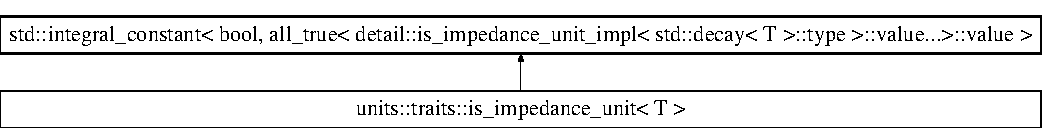
\includegraphics[height=1.715161cm]{structunits_1_1traits_1_1is__impedance__unit}
\end{center}
\end{figure}


\subsection{Detailed Description}
\subsubsection*{template$<$typename... T$>$struct units\+::traits\+::is\+\_\+impedance\+\_\+unit$<$ T $>$}

Trait which tests whether a type represents a unit of impedance. 

Inherits from {\ttfamily std\+::true\+\_\+type} or {\ttfamily std\+::false\+\_\+type}. Use {\ttfamily \hyperlink{structunits_1_1traits_1_1is__impedance__unit}{is\+\_\+impedance\+\_\+unit}$<$T$>$\+::value} to test the unit represents a impedance quantity. 
\begin{DoxyTemplParams}{Template Parameters}
{\em T} & one or more types to test \\
\hline
\end{DoxyTemplParams}


The documentation for this struct was generated from the following file\+:\begin{DoxyCompactItemize}
\item 
/home/nholthaus/workspace/units/include/\hyperlink{units_8h}{units.\+h}\end{DoxyCompactItemize}

\hypertarget{structunits_1_1traits_1_1is__inductance__unit}{}\section{units\+:\+:traits\+:\+:is\+\_\+inductance\+\_\+unit$<$ T $>$ Struct Template Reference}
\label{structunits_1_1traits_1_1is__inductance__unit}\index{units\+::traits\+::is\+\_\+inductance\+\_\+unit$<$ T $>$@{units\+::traits\+::is\+\_\+inductance\+\_\+unit$<$ T $>$}}


Trait which tests whether a type represents a unit of inductance.  




{\ttfamily \#include $<$units.\+h$>$}

Inheritance diagram for units\+:\+:traits\+:\+:is\+\_\+inductance\+\_\+unit$<$ T $>$\+:\begin{figure}[H]
\begin{center}
\leavevmode
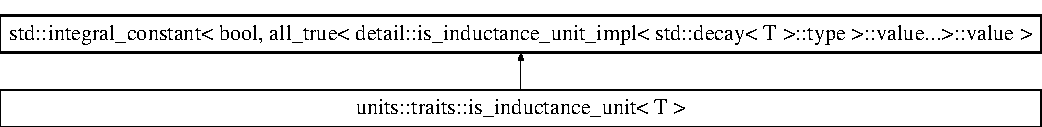
\includegraphics[height=1.712538cm]{structunits_1_1traits_1_1is__inductance__unit}
\end{center}
\end{figure}


\subsection{Detailed Description}
\subsubsection*{template$<$typename... T$>$struct units\+::traits\+::is\+\_\+inductance\+\_\+unit$<$ T $>$}

Trait which tests whether a type represents a unit of inductance. 

Inherits from {\ttfamily std\+::true\+\_\+type} or {\ttfamily std\+::false\+\_\+type}. Use {\ttfamily \hyperlink{structunits_1_1traits_1_1is__inductance__unit}{is\+\_\+inductance\+\_\+unit}$<$T$>$\+::value} to test the unit represents a inductance quantity. 
\begin{DoxyTemplParams}{Template Parameters}
{\em T} & one or more types to test \\
\hline
\end{DoxyTemplParams}


The documentation for this struct was generated from the following file\+:\begin{DoxyCompactItemize}
\item 
/home/nholthaus/workspace/units/include/\hyperlink{units_8h}{units.\+h}\end{DoxyCompactItemize}

\hypertarget{structunits_1_1traits_1_1is__length__unit}{}\section{units\+:\+:traits\+:\+:is\+\_\+length\+\_\+unit$<$ T $>$ Struct Template Reference}
\label{structunits_1_1traits_1_1is__length__unit}\index{units\+::traits\+::is\+\_\+length\+\_\+unit$<$ T $>$@{units\+::traits\+::is\+\_\+length\+\_\+unit$<$ T $>$}}


Trait which tests whether a type represents a unit of length.  




{\ttfamily \#include $<$units.\+h$>$}

Inheritance diagram for units\+:\+:traits\+:\+:is\+\_\+length\+\_\+unit$<$ T $>$\+:\begin{figure}[H]
\begin{center}
\leavevmode
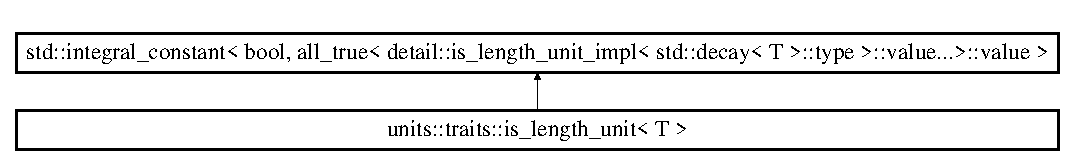
\includegraphics[height=1.789137cm]{structunits_1_1traits_1_1is__length__unit}
\end{center}
\end{figure}


\subsection{Detailed Description}
\subsubsection*{template$<$typename... T$>$struct units\+::traits\+::is\+\_\+length\+\_\+unit$<$ T $>$}

Trait which tests whether a type represents a unit of length. 

Inherits from {\ttfamily std\+::true\+\_\+type} or {\ttfamily std\+::false\+\_\+type}. Use {\ttfamily \hyperlink{structunits_1_1traits_1_1is__length__unit}{is\+\_\+length\+\_\+unit}$<$T$>$\+::value} to test the unit represents a length quantity. 
\begin{DoxyTemplParams}{Template Parameters}
{\em T} & one or more types to test \\
\hline
\end{DoxyTemplParams}


The documentation for this struct was generated from the following file\+:\begin{DoxyCompactItemize}
\item 
/home/nholthaus/workspace/units/include/\hyperlink{units_8h}{units.\+h}\end{DoxyCompactItemize}

\hypertarget{structunits_1_1traits_1_1is__luminous__flux__unit}{}\section{units\+:\+:traits\+:\+:is\+\_\+luminous\+\_\+flux\+\_\+unit$<$ T $>$ Struct Template Reference}
\label{structunits_1_1traits_1_1is__luminous__flux__unit}\index{units\+::traits\+::is\+\_\+luminous\+\_\+flux\+\_\+unit$<$ T $>$@{units\+::traits\+::is\+\_\+luminous\+\_\+flux\+\_\+unit$<$ T $>$}}


Trait which tests whether a type represents a unit of \hyperlink{namespaceunits_1_1luminous__flux}{luminous\+\_\+flux}.  




{\ttfamily \#include $<$units.\+h$>$}

Inheritance diagram for units\+:\+:traits\+:\+:is\+\_\+luminous\+\_\+flux\+\_\+unit$<$ T $>$\+:\begin{figure}[H]
\begin{center}
\leavevmode
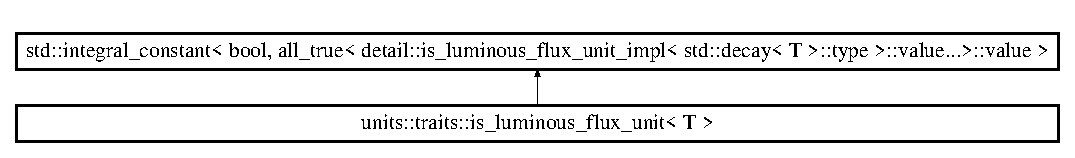
\includegraphics[height=1.676647cm]{structunits_1_1traits_1_1is__luminous__flux__unit}
\end{center}
\end{figure}


\subsection{Detailed Description}
\subsubsection*{template$<$typename... T$>$struct units\+::traits\+::is\+\_\+luminous\+\_\+flux\+\_\+unit$<$ T $>$}

Trait which tests whether a type represents a unit of \hyperlink{namespaceunits_1_1luminous__flux}{luminous\+\_\+flux}. 

Inherits from {\ttfamily std\+::true\+\_\+type} or {\ttfamily std\+::false\+\_\+type}. Use {\ttfamily \hyperlink{structunits_1_1traits_1_1is__luminous__flux__unit}{is\+\_\+luminous\+\_\+flux\+\_\+unit}$<$T$>$\+::value} to test the unit represents a \hyperlink{namespaceunits_1_1luminous__flux}{luminous\+\_\+flux} quantity. 
\begin{DoxyTemplParams}{Template Parameters}
{\em T} & one or more types to test \\
\hline
\end{DoxyTemplParams}


The documentation for this struct was generated from the following file\+:\begin{DoxyCompactItemize}
\item 
/home/nholthaus/workspace/units/include/\hyperlink{units_8h}{units.\+h}\end{DoxyCompactItemize}

\hypertarget{structunits_1_1traits_1_1is__luminous__intensity__unit}{}\section{units\+:\+:traits\+:\+:is\+\_\+luminous\+\_\+intensity\+\_\+unit$<$ T $>$ Struct Template Reference}
\label{structunits_1_1traits_1_1is__luminous__intensity__unit}\index{units\+::traits\+::is\+\_\+luminous\+\_\+intensity\+\_\+unit$<$ T $>$@{units\+::traits\+::is\+\_\+luminous\+\_\+intensity\+\_\+unit$<$ T $>$}}


Trait which tests whether a type represents a unit of \hyperlink{namespaceunits_1_1luminous__intensity}{luminous\+\_\+intensity}.  




{\ttfamily \#include $<$units.\+h$>$}

Inheritance diagram for units\+:\+:traits\+:\+:is\+\_\+luminous\+\_\+intensity\+\_\+unit$<$ T $>$\+:\begin{figure}[H]
\begin{center}
\leavevmode
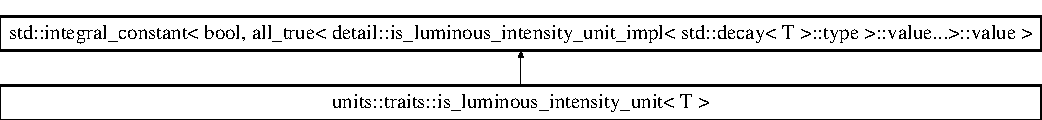
\includegraphics[height=1.613833cm]{structunits_1_1traits_1_1is__luminous__intensity__unit}
\end{center}
\end{figure}


\subsection{Detailed Description}
\subsubsection*{template$<$typename... T$>$struct units\+::traits\+::is\+\_\+luminous\+\_\+intensity\+\_\+unit$<$ T $>$}

Trait which tests whether a type represents a unit of \hyperlink{namespaceunits_1_1luminous__intensity}{luminous\+\_\+intensity}. 

Inherits from {\ttfamily std\+::true\+\_\+type} or {\ttfamily std\+::false\+\_\+type}. Use {\ttfamily \hyperlink{structunits_1_1traits_1_1is__luminous__intensity__unit}{is\+\_\+luminous\+\_\+intensity\+\_\+unit}$<$T$>$\+::value} to test the unit represents a \hyperlink{namespaceunits_1_1luminous__intensity}{luminous\+\_\+intensity} quantity. 
\begin{DoxyTemplParams}{Template Parameters}
{\em T} & one or more types to test \\
\hline
\end{DoxyTemplParams}


The documentation for this struct was generated from the following file\+:\begin{DoxyCompactItemize}
\item 
/home/nholthaus/workspace/units/include/\hyperlink{units_8h}{units.\+h}\end{DoxyCompactItemize}

\hypertarget{structunits_1_1traits_1_1is__magnetic__field__strength__unit}{}\section{units\+:\+:traits\+:\+:is\+\_\+magnetic\+\_\+field\+\_\+strength\+\_\+unit$<$ T $>$ Struct Template Reference}
\label{structunits_1_1traits_1_1is__magnetic__field__strength__unit}\index{units\+::traits\+::is\+\_\+magnetic\+\_\+field\+\_\+strength\+\_\+unit$<$ T $>$@{units\+::traits\+::is\+\_\+magnetic\+\_\+field\+\_\+strength\+\_\+unit$<$ T $>$}}


Trait which tests whether a type represents a unit of \hyperlink{namespaceunits_1_1magnetic__field__strength}{magnetic\+\_\+field\+\_\+strength}.  




{\ttfamily \#include $<$units.\+h$>$}

Inheritance diagram for units\+:\+:traits\+:\+:is\+\_\+magnetic\+\_\+field\+\_\+strength\+\_\+unit$<$ T $>$\+:\begin{figure}[H]
\begin{center}
\leavevmode
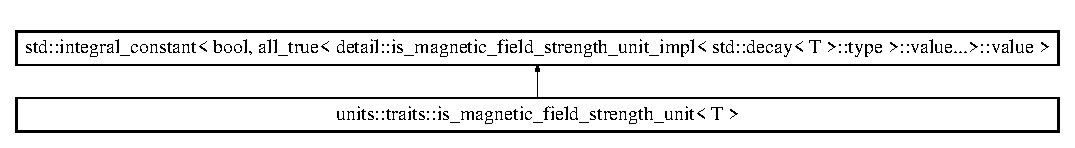
\includegraphics[height=1.544828cm]{structunits_1_1traits_1_1is__magnetic__field__strength__unit}
\end{center}
\end{figure}


\subsection{Detailed Description}
\subsubsection*{template$<$typename... T$>$struct units\+::traits\+::is\+\_\+magnetic\+\_\+field\+\_\+strength\+\_\+unit$<$ T $>$}

Trait which tests whether a type represents a unit of \hyperlink{namespaceunits_1_1magnetic__field__strength}{magnetic\+\_\+field\+\_\+strength}. 

Inherits from {\ttfamily std\+::true\+\_\+type} or {\ttfamily std\+::false\+\_\+type}. Use {\ttfamily \hyperlink{structunits_1_1traits_1_1is__magnetic__field__strength__unit}{is\+\_\+magnetic\+\_\+field\+\_\+strength\+\_\+unit}$<$T$>$\+::value} to test the unit represents a \hyperlink{namespaceunits_1_1magnetic__field__strength}{magnetic\+\_\+field\+\_\+strength} quantity. 
\begin{DoxyTemplParams}{Template Parameters}
{\em T} & one or more types to test \\
\hline
\end{DoxyTemplParams}


The documentation for this struct was generated from the following file\+:\begin{DoxyCompactItemize}
\item 
/home/nholthaus/workspace/units/include/\hyperlink{units_8h}{units.\+h}\end{DoxyCompactItemize}

\hypertarget{structunits_1_1traits_1_1is__magnetic__flux__unit}{}\section{units\+:\+:traits\+:\+:is\+\_\+magnetic\+\_\+flux\+\_\+unit$<$ T $>$ Struct Template Reference}
\label{structunits_1_1traits_1_1is__magnetic__flux__unit}\index{units\+::traits\+::is\+\_\+magnetic\+\_\+flux\+\_\+unit$<$ T $>$@{units\+::traits\+::is\+\_\+magnetic\+\_\+flux\+\_\+unit$<$ T $>$}}


Trait which tests whether a type represents a unit of \hyperlink{namespaceunits_1_1magnetic__flux}{magnetic\+\_\+flux}.  




{\ttfamily \#include $<$units.\+h$>$}

Inheritance diagram for units\+:\+:traits\+:\+:is\+\_\+magnetic\+\_\+flux\+\_\+unit$<$ T $>$\+:\begin{figure}[H]
\begin{center}
\leavevmode
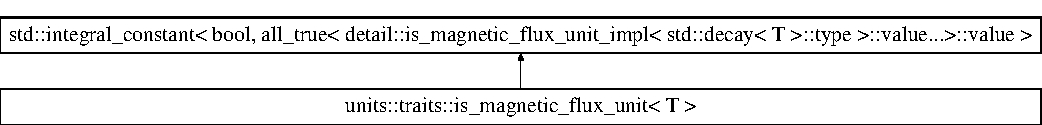
\includegraphics[height=1.674140cm]{structunits_1_1traits_1_1is__magnetic__flux__unit}
\end{center}
\end{figure}


\subsection{Detailed Description}
\subsubsection*{template$<$typename... T$>$struct units\+::traits\+::is\+\_\+magnetic\+\_\+flux\+\_\+unit$<$ T $>$}

Trait which tests whether a type represents a unit of \hyperlink{namespaceunits_1_1magnetic__flux}{magnetic\+\_\+flux}. 

Inherits from {\ttfamily std\+::true\+\_\+type} or {\ttfamily std\+::false\+\_\+type}. Use {\ttfamily \hyperlink{structunits_1_1traits_1_1is__magnetic__flux__unit}{is\+\_\+magnetic\+\_\+flux\+\_\+unit}$<$T$>$\+::value} to test the unit represents a \hyperlink{namespaceunits_1_1magnetic__flux}{magnetic\+\_\+flux} quantity. 
\begin{DoxyTemplParams}{Template Parameters}
{\em T} & one or more types to test \\
\hline
\end{DoxyTemplParams}


The documentation for this struct was generated from the following file\+:\begin{DoxyCompactItemize}
\item 
/home/nholthaus/workspace/units/include/\hyperlink{units_8h}{units.\+h}\end{DoxyCompactItemize}

\hypertarget{structunits_1_1traits_1_1is__mass__unit}{}\section{units\+:\+:traits\+:\+:is\+\_\+mass\+\_\+unit$<$ T $>$ Struct Template Reference}
\label{structunits_1_1traits_1_1is__mass__unit}\index{units\+::traits\+::is\+\_\+mass\+\_\+unit$<$ T $>$@{units\+::traits\+::is\+\_\+mass\+\_\+unit$<$ T $>$}}


Trait which tests whether a type represents a unit of mass.  




{\ttfamily \#include $<$units.\+h$>$}

Inheritance diagram for units\+:\+:traits\+:\+:is\+\_\+mass\+\_\+unit$<$ T $>$\+:\begin{figure}[H]
\begin{center}
\leavevmode
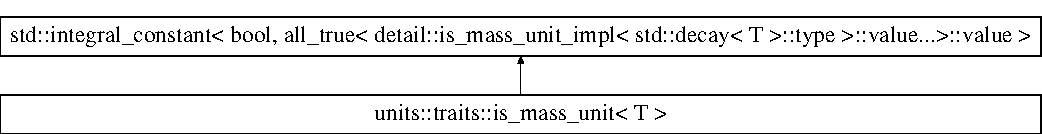
\includegraphics[height=1.806452cm]{structunits_1_1traits_1_1is__mass__unit}
\end{center}
\end{figure}


\subsection{Detailed Description}
\subsubsection*{template$<$typename... T$>$struct units\+::traits\+::is\+\_\+mass\+\_\+unit$<$ T $>$}

Trait which tests whether a type represents a unit of mass. 

Inherits from {\ttfamily std\+::true\+\_\+type} or {\ttfamily std\+::false\+\_\+type}. Use {\ttfamily \hyperlink{structunits_1_1traits_1_1is__mass__unit}{is\+\_\+mass\+\_\+unit}$<$T$>$\+::value} to test the unit represents a mass quantity. 
\begin{DoxyTemplParams}{Template Parameters}
{\em T} & one or more types to test \\
\hline
\end{DoxyTemplParams}


The documentation for this struct was generated from the following file\+:\begin{DoxyCompactItemize}
\item 
/home/nholthaus/workspace/units/include/\hyperlink{units_8h}{units.\+h}\end{DoxyCompactItemize}

\hypertarget{structunits_1_1traits_1_1is__nonlinear__scale}{}\section{units\+:\+:traits\+:\+:is\+\_\+nonlinear\+\_\+scale$<$ T, Ret $>$ Struct Template Reference}
\label{structunits_1_1traits_1_1is__nonlinear__scale}\index{units\+::traits\+::is\+\_\+nonlinear\+\_\+scale$<$ T, Ret $>$@{units\+::traits\+::is\+\_\+nonlinear\+\_\+scale$<$ T, Ret $>$}}


Trait which tests that {\ttfamily class T} meets the requirements for a non-\/linear scale.  




{\ttfamily \#include $<$units.\+h$>$}

Inheritance diagram for units\+:\+:traits\+:\+:is\+\_\+nonlinear\+\_\+scale$<$ T, Ret $>$\+:\begin{figure}[H]
\begin{center}
\leavevmode
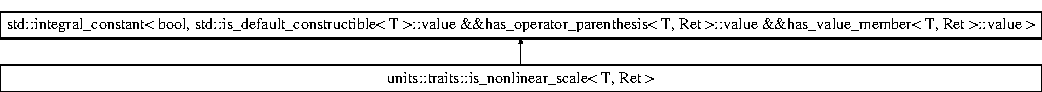
\includegraphics[height=1.230769cm]{structunits_1_1traits_1_1is__nonlinear__scale}
\end{center}
\end{figure}


\subsection{Detailed Description}
\subsubsection*{template$<$class T, class Ret$>$struct units\+::traits\+::is\+\_\+nonlinear\+\_\+scale$<$ T, Ret $>$}

Trait which tests that {\ttfamily class T} meets the requirements for a non-\/linear scale. 

A non-\/linear scale must\+:
\begin{DoxyItemize}
\item be default constructible
\item have an {\ttfamily operator()} member which returns the non-\/linear value stored in the scale
\item have an accessible {\ttfamily m\+\_\+value} member type which stores the linearized value in the scale.
\end{DoxyItemize}

Linear/nonlinear scales are used by {\ttfamily \hyperlink{structunits_1_1unit}{units\+::unit}} to store values and scale them if they represent things like d\+B. 

The documentation for this struct was generated from the following file\+:\begin{DoxyCompactItemize}
\item 
/home/nholthaus/workspace/units/include/\hyperlink{units_8h}{units.\+h}\end{DoxyCompactItemize}

\hypertarget{structunits_1_1traits_1_1is__power__unit}{}\section{units\+:\+:traits\+:\+:is\+\_\+power\+\_\+unit$<$ T $>$ Struct Template Reference}
\label{structunits_1_1traits_1_1is__power__unit}\index{units\+::traits\+::is\+\_\+power\+\_\+unit$<$ T $>$@{units\+::traits\+::is\+\_\+power\+\_\+unit$<$ T $>$}}


Trait which tests whether a type represents a unit of power.  




{\ttfamily \#include $<$units.\+h$>$}

Inheritance diagram for units\+:\+:traits\+:\+:is\+\_\+power\+\_\+unit$<$ T $>$\+:\begin{figure}[H]
\begin{center}
\leavevmode
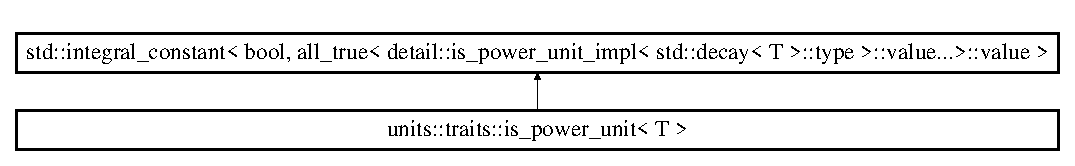
\includegraphics[height=1.786284cm]{structunits_1_1traits_1_1is__power__unit}
\end{center}
\end{figure}


\subsection{Detailed Description}
\subsubsection*{template$<$typename... T$>$struct units\+::traits\+::is\+\_\+power\+\_\+unit$<$ T $>$}

Trait which tests whether a type represents a unit of power. 

Inherits from {\ttfamily std\+::true\+\_\+type} or {\ttfamily std\+::false\+\_\+type}. Use {\ttfamily \hyperlink{structunits_1_1traits_1_1is__power__unit}{is\+\_\+power\+\_\+unit}$<$T$>$\+::value} to test the unit represents a power quantity. 
\begin{DoxyTemplParams}{Template Parameters}
{\em T} & one or more types to test \\
\hline
\end{DoxyTemplParams}


The documentation for this struct was generated from the following file\+:\begin{DoxyCompactItemize}
\item 
/home/nholthaus/workspace/units/include/\hyperlink{units_8h}{units.\+h}\end{DoxyCompactItemize}

\hypertarget{structunits_1_1traits_1_1is__pressure__unit}{}\section{units\+:\+:traits\+:\+:is\+\_\+pressure\+\_\+unit$<$ T $>$ Struct Template Reference}
\label{structunits_1_1traits_1_1is__pressure__unit}\index{units\+::traits\+::is\+\_\+pressure\+\_\+unit$<$ T $>$@{units\+::traits\+::is\+\_\+pressure\+\_\+unit$<$ T $>$}}


Trait which tests whether a type represents a unit of pressure.  




{\ttfamily \#include $<$units.\+h$>$}

Inheritance diagram for units\+:\+:traits\+:\+:is\+\_\+pressure\+\_\+unit$<$ T $>$\+:\begin{figure}[H]
\begin{center}
\leavevmode
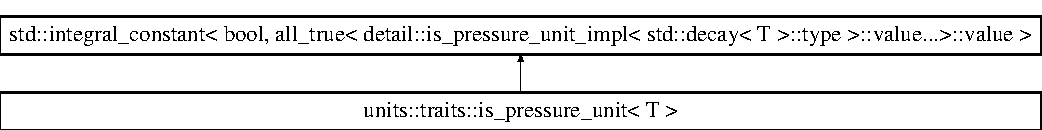
\includegraphics[height=1.744548cm]{structunits_1_1traits_1_1is__pressure__unit}
\end{center}
\end{figure}


\subsection{Detailed Description}
\subsubsection*{template$<$typename... T$>$struct units\+::traits\+::is\+\_\+pressure\+\_\+unit$<$ T $>$}

Trait which tests whether a type represents a unit of pressure. 

Inherits from {\ttfamily std\+::true\+\_\+type} or {\ttfamily std\+::false\+\_\+type}. Use {\ttfamily \hyperlink{structunits_1_1traits_1_1is__pressure__unit}{is\+\_\+pressure\+\_\+unit}$<$T$>$\+::value} to test the unit represents a pressure quantity. 
\begin{DoxyTemplParams}{Template Parameters}
{\em T} & one or more types to test \\
\hline
\end{DoxyTemplParams}


The documentation for this struct was generated from the following file\+:\begin{DoxyCompactItemize}
\item 
/home/nholthaus/workspace/units/include/\hyperlink{units_8h}{units.\+h}\end{DoxyCompactItemize}

\hypertarget{structunits_1_1traits_1_1is__radioactivity__unit}{}\section{units\+:\+:traits\+:\+:is\+\_\+radioactivity\+\_\+unit$<$ T $>$ Struct Template Reference}
\label{structunits_1_1traits_1_1is__radioactivity__unit}\index{units\+::traits\+::is\+\_\+radioactivity\+\_\+unit$<$ T $>$@{units\+::traits\+::is\+\_\+radioactivity\+\_\+unit$<$ T $>$}}


Trait which tests whether a type represents a unit of radiation.  




{\ttfamily \#include $<$units.\+h$>$}

Inheritance diagram for units\+:\+:traits\+:\+:is\+\_\+radioactivity\+\_\+unit$<$ T $>$\+:\begin{figure}[H]
\begin{center}
\leavevmode
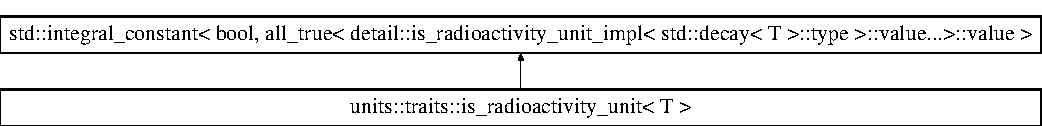
\includegraphics[height=1.694402cm]{structunits_1_1traits_1_1is__radioactivity__unit}
\end{center}
\end{figure}


\subsection{Detailed Description}
\subsubsection*{template$<$typename... T$>$struct units\+::traits\+::is\+\_\+radioactivity\+\_\+unit$<$ T $>$}

Trait which tests whether a type represents a unit of radiation. 

Inherits from {\ttfamily std\+::true\+\_\+type} or {\ttfamily std\+::false\+\_\+type}. Use {\ttfamily \hyperlink{structunits_1_1traits_1_1is__radioactivity__unit}{is\+\_\+radioactivity\+\_\+unit}$<$T$>$\+::value} to test the unit represents a radiation quantity. 
\begin{DoxyTemplParams}{Template Parameters}
{\em T} & one or more types to test \\
\hline
\end{DoxyTemplParams}


The documentation for this struct was generated from the following file\+:\begin{DoxyCompactItemize}
\item 
/home/nholthaus/workspace/units/include/\hyperlink{units_8h}{units.\+h}\end{DoxyCompactItemize}

\hypertarget{structunits_1_1traits_1_1is__ratio}{}\section{units\+:\+:traits\+:\+:is\+\_\+ratio$<$ T $>$ Struct Template Reference}
\label{structunits_1_1traits_1_1is__ratio}\index{units\+::traits\+::is\+\_\+ratio$<$ T $>$@{units\+::traits\+::is\+\_\+ratio$<$ T $>$}}


Trait that tests whether a type represents a std\+::ratio.  




{\ttfamily \#include $<$units.\+h$>$}

Inheritance diagram for units\+:\+:traits\+:\+:is\+\_\+ratio$<$ T $>$\+:\begin{figure}[H]
\begin{center}
\leavevmode
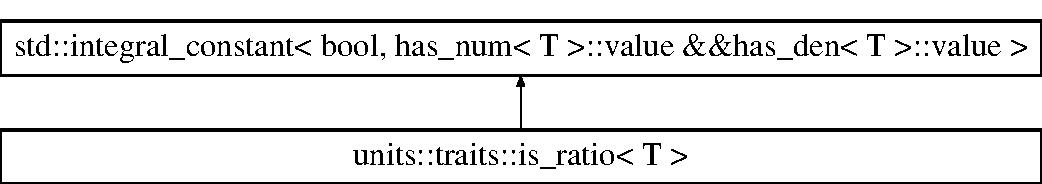
\includegraphics[height=2.000000cm]{structunits_1_1traits_1_1is__ratio}
\end{center}
\end{figure}


\subsection{Detailed Description}
\subsubsection*{template$<$class T$>$struct units\+::traits\+::is\+\_\+ratio$<$ T $>$}

Trait that tests whether a type represents a std\+::ratio. 

Inherits from {\ttfamily std\+::true\+\_\+type} or {\ttfamily std\+::false\+\_\+type}. Use {\ttfamily \hyperlink{structunits_1_1traits_1_1is__ratio}{is\+\_\+ratio}$<$T$>$\+::value} to test whether {\ttfamily class T} implements a std\+::ratio. 

The documentation for this struct was generated from the following file\+:\begin{DoxyCompactItemize}
\item 
/home/nholthaus/workspace/units/include/\hyperlink{units_8h}{units.\+h}\end{DoxyCompactItemize}

\hypertarget{structunits_1_1traits_1_1is__same__scale}{}\section{units\+:\+:traits\+:\+:is\+\_\+same\+\_\+scale$<$ T1, T2 $>$ Struct Template Reference}
\label{structunits_1_1traits_1_1is__same__scale}\index{units\+::traits\+::is\+\_\+same\+\_\+scale$<$ T1, T2 $>$@{units\+::traits\+::is\+\_\+same\+\_\+scale$<$ T1, T2 $>$}}


Trait which tests whether two types has the same non-\/linear scale.  




{\ttfamily \#include $<$units.\+h$>$}

Inheritance diagram for units\+:\+:traits\+:\+:is\+\_\+same\+\_\+scale$<$ T1, T2 $>$\+:\begin{figure}[H]
\begin{center}
\leavevmode
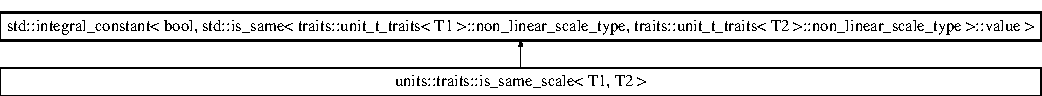
\includegraphics[height=1.287356cm]{structunits_1_1traits_1_1is__same__scale}
\end{center}
\end{figure}


\subsection{Detailed Description}
\subsubsection*{template$<$typename T1, typename T2$>$struct units\+::traits\+::is\+\_\+same\+\_\+scale$<$ T1, T2 $>$}

Trait which tests whether two types has the same non-\/linear scale. 

Inherits from {\ttfamily std\+::true\+\_\+type} or {\ttfamily std\+::false\+\_\+type}. Use {\ttfamily \hyperlink{structunits_1_1traits_1_1is__same__scale}{is\+\_\+same\+\_\+scale}$<$U1 , U2$>$\+::value} to test whether two types have the same non-\/linear scale. 
\begin{DoxyTemplParams}{Template Parameters}
{\em T1} & left hand type. \\
\hline
{\em T2} & right hand type \\
\hline
\end{DoxyTemplParams}


The documentation for this struct was generated from the following file\+:\begin{DoxyCompactItemize}
\item 
/home/nholthaus/workspace/units/include/\hyperlink{units_8h}{units.\+h}\end{DoxyCompactItemize}

\hypertarget{structunits_1_1traits_1_1is__scalar__unit}{}\section{units\+:\+:traits\+:\+:is\+\_\+scalar\+\_\+unit$<$ T $>$ Struct Template Reference}
\label{structunits_1_1traits_1_1is__scalar__unit}\index{units\+::traits\+::is\+\_\+scalar\+\_\+unit$<$ T $>$@{units\+::traits\+::is\+\_\+scalar\+\_\+unit$<$ T $>$}}


Trait which tests whether one or more types derived from {\ttfamily \hyperlink{classunits_1_1unit__t}{unit\+\_\+t}} represent scalar values.  




{\ttfamily \#include $<$units.\+h$>$}

Inheritance diagram for units\+:\+:traits\+:\+:is\+\_\+scalar\+\_\+unit$<$ T $>$\+:\begin{figure}[H]
\begin{center}
\leavevmode
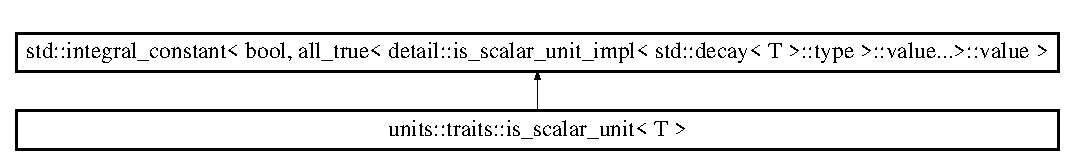
\includegraphics[height=1.786284cm]{structunits_1_1traits_1_1is__scalar__unit}
\end{center}
\end{figure}


\subsection{Detailed Description}
\subsubsection*{template$<$class... T$>$struct units\+::traits\+::is\+\_\+scalar\+\_\+unit$<$ T $>$}

Trait which tests whether one or more types derived from {\ttfamily \hyperlink{classunits_1_1unit__t}{unit\+\_\+t}} represent scalar values. 

Inherits from {\ttfamily std\+::true\+\_\+type} or {\ttfamily std\+::false\+\_\+type}. Use {\ttfamily \hyperlink{structunits_1_1traits_1_1is__scalar__unit}{is\+\_\+scalar\+\_\+unit}$<$U1 \mbox{[}, U2, ...\mbox{]}$>$\+::value} to test one or more types to see if they represent scalar value containers. A scalar unit is one which has no dimensions (e.\+g. P\+I). 
\begin{DoxyTemplParams}{Template Parameters}
{\em T} & one or more types to test. \\
\hline
\end{DoxyTemplParams}


The documentation for this struct was generated from the following file\+:\begin{DoxyCompactItemize}
\item 
/home/nholthaus/workspace/units/include/\hyperlink{units_8h}{units.\+h}\end{DoxyCompactItemize}

\hypertarget{structunits_1_1traits_1_1is__solid__angle__unit}{}\section{units\+:\+:traits\+:\+:is\+\_\+solid\+\_\+angle\+\_\+unit$<$ T $>$ Struct Template Reference}
\label{structunits_1_1traits_1_1is__solid__angle__unit}\index{units\+::traits\+::is\+\_\+solid\+\_\+angle\+\_\+unit$<$ T $>$@{units\+::traits\+::is\+\_\+solid\+\_\+angle\+\_\+unit$<$ T $>$}}


Trait which tests whether a type represents a unit of \hyperlink{namespaceunits_1_1solid__angle}{solid\+\_\+angle}.  




{\ttfamily \#include $<$units.\+h$>$}

Inheritance diagram for units\+:\+:traits\+:\+:is\+\_\+solid\+\_\+angle\+\_\+unit$<$ T $>$\+:\begin{figure}[H]
\begin{center}
\leavevmode
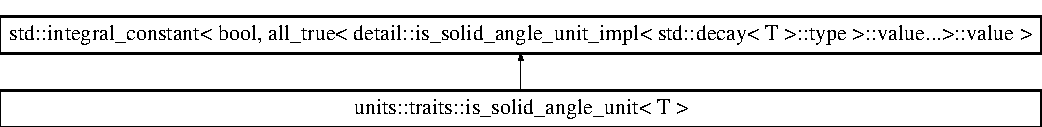
\includegraphics[height=1.707317cm]{structunits_1_1traits_1_1is__solid__angle__unit}
\end{center}
\end{figure}


\subsection{Detailed Description}
\subsubsection*{template$<$typename... T$>$struct units\+::traits\+::is\+\_\+solid\+\_\+angle\+\_\+unit$<$ T $>$}

Trait which tests whether a type represents a unit of \hyperlink{namespaceunits_1_1solid__angle}{solid\+\_\+angle}. 

Inherits from {\ttfamily std\+::true\+\_\+type} or {\ttfamily std\+::false\+\_\+type}. Use {\ttfamily \hyperlink{structunits_1_1traits_1_1is__solid__angle__unit}{is\+\_\+solid\+\_\+angle\+\_\+unit}$<$T$>$\+::value} to test the unit represents a \hyperlink{namespaceunits_1_1solid__angle}{solid\+\_\+angle} quantity. 
\begin{DoxyTemplParams}{Template Parameters}
{\em T} & one or more types to test \\
\hline
\end{DoxyTemplParams}


The documentation for this struct was generated from the following file\+:\begin{DoxyCompactItemize}
\item 
/home/nholthaus/workspace/units/include/\hyperlink{units_8h}{units.\+h}\end{DoxyCompactItemize}

\hypertarget{structunits_1_1traits_1_1is__substance__unit}{}\section{units\+:\+:traits\+:\+:is\+\_\+substance\+\_\+unit$<$ T $>$ Struct Template Reference}
\label{structunits_1_1traits_1_1is__substance__unit}\index{units\+::traits\+::is\+\_\+substance\+\_\+unit$<$ T $>$@{units\+::traits\+::is\+\_\+substance\+\_\+unit$<$ T $>$}}


Trait which tests whether a type represents a unit of substance.  




{\ttfamily \#include $<$units.\+h$>$}

Inheritance diagram for units\+:\+:traits\+:\+:is\+\_\+substance\+\_\+unit$<$ T $>$\+:\begin{figure}[H]
\begin{center}
\leavevmode
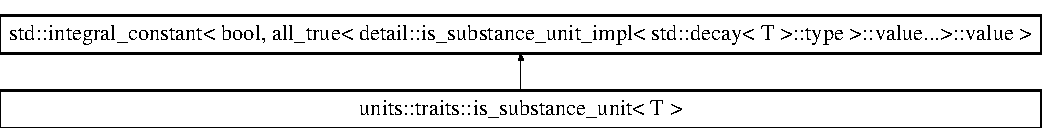
\includegraphics[height=1.725732cm]{structunits_1_1traits_1_1is__substance__unit}
\end{center}
\end{figure}


\subsection{Detailed Description}
\subsubsection*{template$<$typename... T$>$struct units\+::traits\+::is\+\_\+substance\+\_\+unit$<$ T $>$}

Trait which tests whether a type represents a unit of substance. 

Inherits from {\ttfamily std\+::true\+\_\+type} or {\ttfamily std\+::false\+\_\+type}. Use {\ttfamily \hyperlink{structunits_1_1traits_1_1is__substance__unit}{is\+\_\+substance\+\_\+unit}$<$T$>$\+::value} to test the unit represents a substance quantity. 
\begin{DoxyTemplParams}{Template Parameters}
{\em T} & one or more types to test \\
\hline
\end{DoxyTemplParams}


The documentation for this struct was generated from the following file\+:\begin{DoxyCompactItemize}
\item 
/home/nholthaus/workspace/units/include/\hyperlink{units_8h}{units.\+h}\end{DoxyCompactItemize}

\hypertarget{structunits_1_1traits_1_1is__temperature__unit}{}\section{units\+:\+:traits\+:\+:is\+\_\+temperature\+\_\+unit$<$ T $>$ Struct Template Reference}
\label{structunits_1_1traits_1_1is__temperature__unit}\index{units\+::traits\+::is\+\_\+temperature\+\_\+unit$<$ T $>$@{units\+::traits\+::is\+\_\+temperature\+\_\+unit$<$ T $>$}}


Trait which tests whether a type represents a unit of temperature.  




{\ttfamily \#include $<$units.\+h$>$}

Inheritance diagram for units\+:\+:traits\+:\+:is\+\_\+temperature\+\_\+unit$<$ T $>$\+:\begin{figure}[H]
\begin{center}
\leavevmode
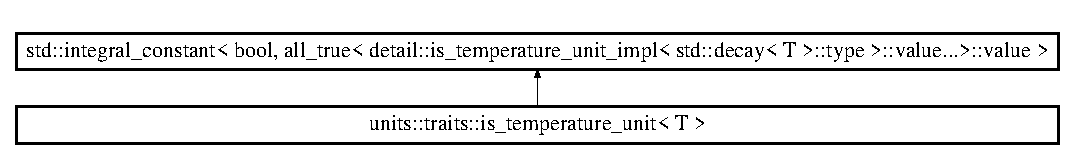
\includegraphics[height=1.699545cm]{structunits_1_1traits_1_1is__temperature__unit}
\end{center}
\end{figure}


\subsection{Detailed Description}
\subsubsection*{template$<$typename... T$>$struct units\+::traits\+::is\+\_\+temperature\+\_\+unit$<$ T $>$}

Trait which tests whether a type represents a unit of temperature. 

Inherits from {\ttfamily std\+::true\+\_\+type} or {\ttfamily std\+::false\+\_\+type}. Use {\ttfamily \hyperlink{structunits_1_1traits_1_1is__temperature__unit}{is\+\_\+temperature\+\_\+unit}$<$T$>$\+::value} to test the unit represents a temperature quantity. 
\begin{DoxyTemplParams}{Template Parameters}
{\em T} & one or more types to test \\
\hline
\end{DoxyTemplParams}


The documentation for this struct was generated from the following file\+:\begin{DoxyCompactItemize}
\item 
/home/nholthaus/workspace/units/include/\hyperlink{units_8h}{units.\+h}\end{DoxyCompactItemize}

\hypertarget{structunits_1_1traits_1_1is__time__unit}{}\section{units\+:\+:traits\+:\+:is\+\_\+time\+\_\+unit$<$ T $>$ Struct Template Reference}
\label{structunits_1_1traits_1_1is__time__unit}\index{units\+::traits\+::is\+\_\+time\+\_\+unit$<$ T $>$@{units\+::traits\+::is\+\_\+time\+\_\+unit$<$ T $>$}}


Trait which tests whether a type represents a unit of time.  




{\ttfamily \#include $<$units.\+h$>$}

Inheritance diagram for units\+:\+:traits\+:\+:is\+\_\+time\+\_\+unit$<$ T $>$\+:\begin{figure}[H]
\begin{center}
\leavevmode
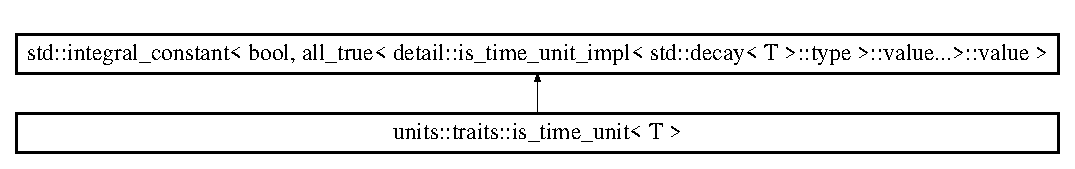
\includegraphics[height=1.824104cm]{structunits_1_1traits_1_1is__time__unit}
\end{center}
\end{figure}


\subsection{Detailed Description}
\subsubsection*{template$<$typename... T$>$struct units\+::traits\+::is\+\_\+time\+\_\+unit$<$ T $>$}

Trait which tests whether a type represents a unit of time. 

Inherits from {\ttfamily std\+::true\+\_\+type} or {\ttfamily std\+::false\+\_\+type}. Use {\ttfamily \hyperlink{structunits_1_1traits_1_1is__time__unit}{is\+\_\+time\+\_\+unit}$<$T$>$\+::value} to test the unit represents a time quantity. 
\begin{DoxyTemplParams}{Template Parameters}
{\em T} & one or more types to test \\
\hline
\end{DoxyTemplParams}


The documentation for this struct was generated from the following file\+:\begin{DoxyCompactItemize}
\item 
/home/nholthaus/workspace/units/include/\hyperlink{units_8h}{units.\+h}\end{DoxyCompactItemize}

\hypertarget{structunits_1_1traits_1_1is__torque__unit}{}\section{units\+:\+:traits\+:\+:is\+\_\+torque\+\_\+unit$<$ T $>$ Struct Template Reference}
\label{structunits_1_1traits_1_1is__torque__unit}\index{units\+::traits\+::is\+\_\+torque\+\_\+unit$<$ T $>$@{units\+::traits\+::is\+\_\+torque\+\_\+unit$<$ T $>$}}


Trait which tests whether a type represents a unit of torque.  




{\ttfamily \#include $<$units.\+h$>$}

Inheritance diagram for units\+:\+:traits\+:\+:is\+\_\+torque\+\_\+unit$<$ T $>$\+:\begin{figure}[H]
\begin{center}
\leavevmode
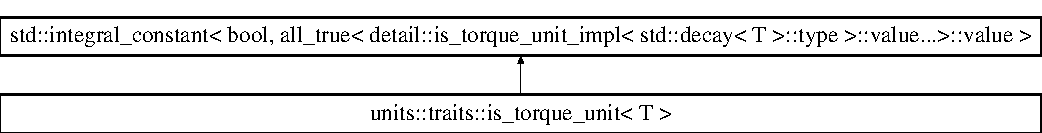
\includegraphics[height=1.786284cm]{structunits_1_1traits_1_1is__torque__unit}
\end{center}
\end{figure}


\subsection{Detailed Description}
\subsubsection*{template$<$typename... T$>$struct units\+::traits\+::is\+\_\+torque\+\_\+unit$<$ T $>$}

Trait which tests whether a type represents a unit of torque. 

Inherits from {\ttfamily std\+::true\+\_\+type} or {\ttfamily std\+::false\+\_\+type}. Use {\ttfamily \hyperlink{structunits_1_1traits_1_1is__torque__unit}{is\+\_\+torque\+\_\+unit}$<$T$>$\+::value} to test the unit represents a torque quantity. 
\begin{DoxyTemplParams}{Template Parameters}
{\em T} & one or more types to test \\
\hline
\end{DoxyTemplParams}


The documentation for this struct was generated from the following file\+:\begin{DoxyCompactItemize}
\item 
/home/nholthaus/workspace/units/include/\hyperlink{units_8h}{units.\+h}\end{DoxyCompactItemize}

\hypertarget{structunits_1_1traits_1_1is__unit}{}\section{units\+:\+:traits\+:\+:is\+\_\+unit$<$ T $>$ Struct Template Reference}
\label{structunits_1_1traits_1_1is__unit}\index{units\+::traits\+::is\+\_\+unit$<$ T $>$@{units\+::traits\+::is\+\_\+unit$<$ T $>$}}


Traits which tests if a class is a {\ttfamily unit}  




{\ttfamily \#include $<$units.\+h$>$}

Inheritance diagram for units\+:\+:traits\+:\+:is\+\_\+unit$<$ T $>$\+:\begin{figure}[H]
\begin{center}
\leavevmode
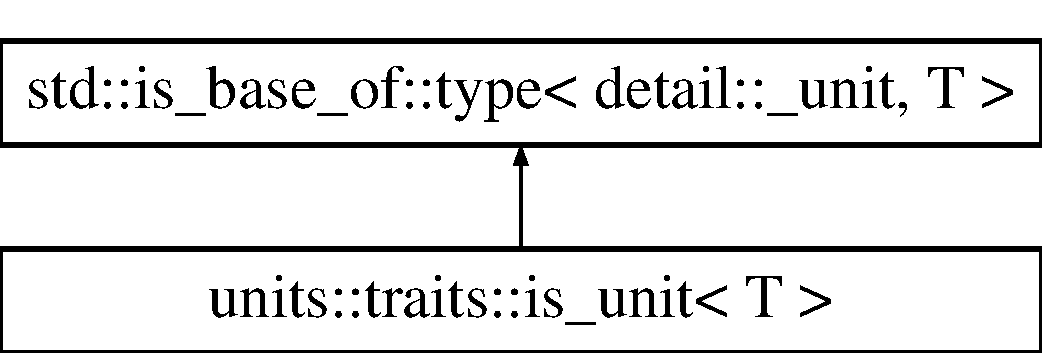
\includegraphics[height=2.000000cm]{structunits_1_1traits_1_1is__unit}
\end{center}
\end{figure}


\subsection{Detailed Description}
\subsubsection*{template$<$class T$>$struct units\+::traits\+::is\+\_\+unit$<$ T $>$}

Traits which tests if a class is a {\ttfamily unit} 

Inherits from {\ttfamily std\+::true\+\_\+type} or {\ttfamily std\+::false\+\_\+type}. Use {\ttfamily \hyperlink{structunits_1_1traits_1_1is__unit}{is\+\_\+unit}$<$T$>$\+::value} to test whether {\ttfamily class T} implements a {\ttfamily unit}. 

The documentation for this struct was generated from the following file\+:\begin{DoxyCompactItemize}
\item 
/home/nholthaus/workspace/units/include/\hyperlink{units_8h}{units.\+h}\end{DoxyCompactItemize}

\hypertarget{structunits_1_1traits_1_1is__unit__t}{}\section{units\+:\+:traits\+:\+:is\+\_\+unit\+\_\+t$<$ T $>$ Struct Template Reference}
\label{structunits_1_1traits_1_1is__unit__t}\index{units\+::traits\+::is\+\_\+unit\+\_\+t$<$ T $>$@{units\+::traits\+::is\+\_\+unit\+\_\+t$<$ T $>$}}


Traits which tests if a class is a {\ttfamily unit}  




{\ttfamily \#include $<$units.\+h$>$}

Inheritance diagram for units\+:\+:traits\+:\+:is\+\_\+unit\+\_\+t$<$ T $>$\+:\begin{figure}[H]
\begin{center}
\leavevmode
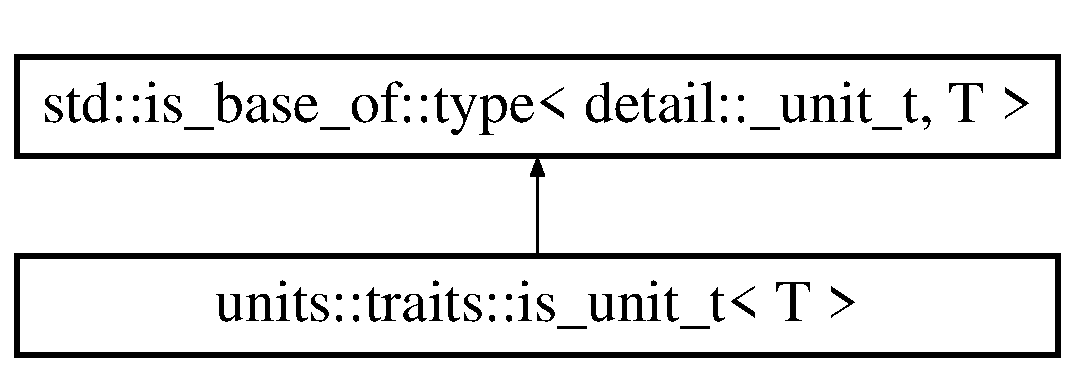
\includegraphics[height=2.000000cm]{structunits_1_1traits_1_1is__unit__t}
\end{center}
\end{figure}


\subsection{Detailed Description}
\subsubsection*{template$<$class T$>$struct units\+::traits\+::is\+\_\+unit\+\_\+t$<$ T $>$}

Traits which tests if a class is a {\ttfamily unit} 

Inherits from {\ttfamily std\+::true\+\_\+type} or {\ttfamily std\+::false\+\_\+type}. Use {\ttfamily \hyperlink{structunits_1_1traits_1_1is__unit}{is\+\_\+unit}$<$T$>$\+::value} to test whether {\ttfamily class T} implements a {\ttfamily unit}. 

The documentation for this struct was generated from the following file\+:\begin{DoxyCompactItemize}
\item 
/home/nholthaus/workspace/units/include/\hyperlink{units_8h}{units.\+h}\end{DoxyCompactItemize}

\hypertarget{structunits_1_1traits_1_1is__unit__value__t}{}\section{units\+:\+:traits\+:\+:is\+\_\+unit\+\_\+value\+\_\+t$<$ T, Units $>$ Struct Template Reference}
\label{structunits_1_1traits_1_1is__unit__value__t}\index{units\+::traits\+::is\+\_\+unit\+\_\+value\+\_\+t$<$ T, Units $>$@{units\+::traits\+::is\+\_\+unit\+\_\+value\+\_\+t$<$ T, Units $>$}}


Trait which tests whether a type is a \hyperlink{structunits_1_1unit__value__t}{unit\+\_\+value\+\_\+t} representing the given unit type.  




{\ttfamily \#include $<$units.\+h$>$}

Inheritance diagram for units\+:\+:traits\+:\+:is\+\_\+unit\+\_\+value\+\_\+t$<$ T, Units $>$\+:\begin{figure}[H]
\begin{center}
\leavevmode
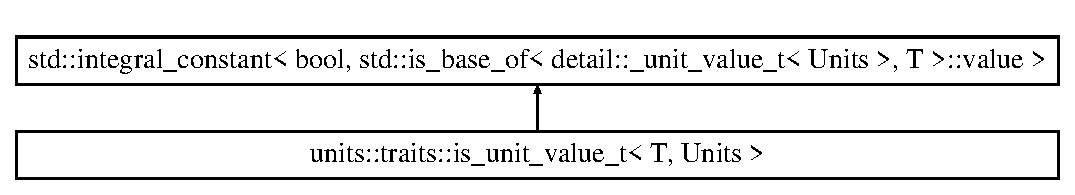
\includegraphics[height=2.000000cm]{structunits_1_1traits_1_1is__unit__value__t}
\end{center}
\end{figure}


\subsection{Detailed Description}
\subsubsection*{template$<$typename T, typename Units = typename traits\+::unit\+\_\+value\+\_\+t\+\_\+traits$<$\+T$>$\+::unit\+\_\+type$>$struct units\+::traits\+::is\+\_\+unit\+\_\+value\+\_\+t$<$ T, Units $>$}

Trait which tests whether a type is a \hyperlink{structunits_1_1unit__value__t}{unit\+\_\+value\+\_\+t} representing the given unit type. 

e.\+g. {\ttfamily \hyperlink{structunits_1_1traits_1_1is__unit__value__t}{is\+\_\+unit\+\_\+value\+\_\+t}$<$meters, my\+Type$>$\+::value} would test that {\ttfamily my\+Type} is a {\ttfamily \hyperlink{structunits_1_1unit__value__t}{unit\+\_\+value\+\_\+t}$<$meters$>$}. 
\begin{DoxyTemplParams}{Template Parameters}
{\em Units} & units that the {\ttfamily \hyperlink{structunits_1_1unit__value__t}{unit\+\_\+value\+\_\+t}} is supposed to have. \\
\hline
{\em T} & type to test. \\
\hline
\end{DoxyTemplParams}


The documentation for this struct was generated from the following file\+:\begin{DoxyCompactItemize}
\item 
/home/nholthaus/workspace/units/include/\hyperlink{units_8h}{units.\+h}\end{DoxyCompactItemize}

\hypertarget{structunits_1_1traits_1_1is__unit__value__t__category}{}\section{units\+:\+:traits\+:\+:is\+\_\+unit\+\_\+value\+\_\+t\+\_\+category$<$ Category, T $>$ Struct Template Reference}
\label{structunits_1_1traits_1_1is__unit__value__t__category}\index{units\+::traits\+::is\+\_\+unit\+\_\+value\+\_\+t\+\_\+category$<$ Category, T $>$@{units\+::traits\+::is\+\_\+unit\+\_\+value\+\_\+t\+\_\+category$<$ Category, T $>$}}


Trait which tests whether type T is a \hyperlink{structunits_1_1unit__value__t}{unit\+\_\+value\+\_\+t} with a unit type in the given category.  




{\ttfamily \#include $<$units.\+h$>$}

Inheritance diagram for units\+:\+:traits\+:\+:is\+\_\+unit\+\_\+value\+\_\+t\+\_\+category$<$ Category, T $>$\+:\begin{figure}[H]
\begin{center}
\leavevmode
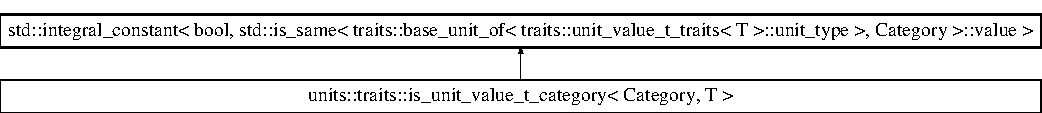
\includegraphics[height=1.521739cm]{structunits_1_1traits_1_1is__unit__value__t__category}
\end{center}
\end{figure}


\subsection{Detailed Description}
\subsubsection*{template$<$typename Category, typename T$>$struct units\+::traits\+::is\+\_\+unit\+\_\+value\+\_\+t\+\_\+category$<$ Category, T $>$}

Trait which tests whether type T is a \hyperlink{structunits_1_1unit__value__t}{unit\+\_\+value\+\_\+t} with a unit type in the given category. 

e.\+g. {\ttfamily \hyperlink{structunits_1_1traits_1_1is__unit__value__t__category}{is\+\_\+unit\+\_\+value\+\_\+t\+\_\+category}$<$units\+::category\+::length, \hyperlink{structunits_1_1unit__value__t}{unit\+\_\+value\+\_\+t}$<$feet$>$$>$\+::value} would be true 

The documentation for this struct was generated from the following file\+:\begin{DoxyCompactItemize}
\item 
/home/nholthaus/workspace/units/include/\hyperlink{units_8h}{units.\+h}\end{DoxyCompactItemize}

\hypertarget{structunits_1_1traits_1_1is__velocity__unit}{}\section{units\+:\+:traits\+:\+:is\+\_\+velocity\+\_\+unit$<$ T $>$ Struct Template Reference}
\label{structunits_1_1traits_1_1is__velocity__unit}\index{units\+::traits\+::is\+\_\+velocity\+\_\+unit$<$ T $>$@{units\+::traits\+::is\+\_\+velocity\+\_\+unit$<$ T $>$}}


Trait which tests whether a type represents a unit of velocity.  




{\ttfamily \#include $<$units.\+h$>$}

Inheritance diagram for units\+:\+:traits\+:\+:is\+\_\+velocity\+\_\+unit$<$ T $>$\+:\begin{figure}[H]
\begin{center}
\leavevmode
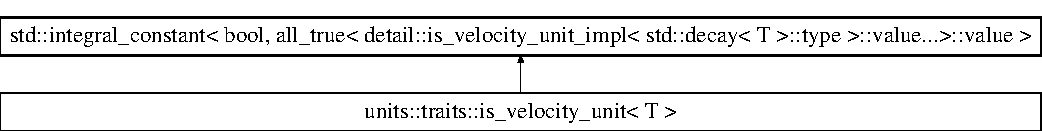
\includegraphics[height=1.761006cm]{structunits_1_1traits_1_1is__velocity__unit}
\end{center}
\end{figure}


\subsection{Detailed Description}
\subsubsection*{template$<$typename... T$>$struct units\+::traits\+::is\+\_\+velocity\+\_\+unit$<$ T $>$}

Trait which tests whether a type represents a unit of velocity. 

Inherits from {\ttfamily std\+::true\+\_\+type} or {\ttfamily std\+::false\+\_\+type}. Use {\ttfamily \hyperlink{structunits_1_1traits_1_1is__velocity__unit}{is\+\_\+velocity\+\_\+unit}$<$T$>$\+::value} to test the unit represents a velocity quantity. 
\begin{DoxyTemplParams}{Template Parameters}
{\em T} & one or more types to test \\
\hline
\end{DoxyTemplParams}


The documentation for this struct was generated from the following file\+:\begin{DoxyCompactItemize}
\item 
/home/nholthaus/workspace/units/include/\hyperlink{units_8h}{units.\+h}\end{DoxyCompactItemize}

\hypertarget{structunits_1_1traits_1_1is__voltage__unit}{}\section{units\+:\+:traits\+:\+:is\+\_\+voltage\+\_\+unit$<$ T $>$ Struct Template Reference}
\label{structunits_1_1traits_1_1is__voltage__unit}\index{units\+::traits\+::is\+\_\+voltage\+\_\+unit$<$ T $>$@{units\+::traits\+::is\+\_\+voltage\+\_\+unit$<$ T $>$}}


Trait which tests whether a type represents a unit of voltage.  




{\ttfamily \#include $<$units.\+h$>$}

Inheritance diagram for units\+:\+:traits\+:\+:is\+\_\+voltage\+\_\+unit$<$ T $>$\+:\begin{figure}[H]
\begin{center}
\leavevmode
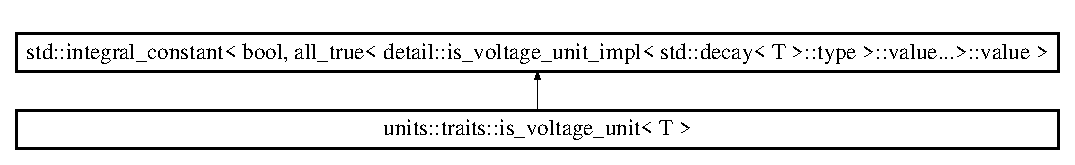
\includegraphics[height=1.769352cm]{structunits_1_1traits_1_1is__voltage__unit}
\end{center}
\end{figure}


\subsection{Detailed Description}
\subsubsection*{template$<$typename... T$>$struct units\+::traits\+::is\+\_\+voltage\+\_\+unit$<$ T $>$}

Trait which tests whether a type represents a unit of voltage. 

Inherits from {\ttfamily std\+::true\+\_\+type} or {\ttfamily std\+::false\+\_\+type}. Use {\ttfamily \hyperlink{structunits_1_1traits_1_1is__voltage__unit}{is\+\_\+voltage\+\_\+unit}$<$T$>$\+::value} to test the unit represents a voltage quantity. 
\begin{DoxyTemplParams}{Template Parameters}
{\em T} & one or more types to test \\
\hline
\end{DoxyTemplParams}


The documentation for this struct was generated from the following file\+:\begin{DoxyCompactItemize}
\item 
/home/nholthaus/workspace/units/include/\hyperlink{units_8h}{units.\+h}\end{DoxyCompactItemize}

\hypertarget{structunits_1_1traits_1_1is__volume__unit}{}\section{units\+:\+:traits\+:\+:is\+\_\+volume\+\_\+unit$<$ T $>$ Struct Template Reference}
\label{structunits_1_1traits_1_1is__volume__unit}\index{units\+::traits\+::is\+\_\+volume\+\_\+unit$<$ T $>$@{units\+::traits\+::is\+\_\+volume\+\_\+unit$<$ T $>$}}


Trait which tests whether a type represents a unit of volume.  




{\ttfamily \#include $<$units.\+h$>$}

Inheritance diagram for units\+:\+:traits\+:\+:is\+\_\+volume\+\_\+unit$<$ T $>$\+:\begin{figure}[H]
\begin{center}
\leavevmode
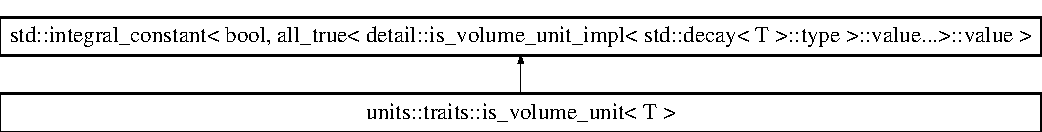
\includegraphics[height=1.772152cm]{structunits_1_1traits_1_1is__volume__unit}
\end{center}
\end{figure}


\subsection{Detailed Description}
\subsubsection*{template$<$typename... T$>$struct units\+::traits\+::is\+\_\+volume\+\_\+unit$<$ T $>$}

Trait which tests whether a type represents a unit of volume. 

Inherits from {\ttfamily std\+::true\+\_\+type} or {\ttfamily std\+::false\+\_\+type}. Use {\ttfamily \hyperlink{structunits_1_1traits_1_1is__volume__unit}{is\+\_\+volume\+\_\+unit}$<$T$>$\+::value} to test the unit represents a volume quantity. 
\begin{DoxyTemplParams}{Template Parameters}
{\em T} & one or more types to test \\
\hline
\end{DoxyTemplParams}


The documentation for this struct was generated from the following file\+:\begin{DoxyCompactItemize}
\item 
/home/nholthaus/workspace/units/include/\hyperlink{units_8h}{units.\+h}\end{DoxyCompactItemize}

\hypertarget{structunits_1_1linear__scale}{}\section{units\+:\+:linear\+\_\+scale$<$ T $>$ Struct Template Reference}
\label{structunits_1_1linear__scale}\index{units\+::linear\+\_\+scale$<$ T $>$@{units\+::linear\+\_\+scale$<$ T $>$}}


\hyperlink{classunits_1_1unit__t}{unit\+\_\+t} scale which is linear  




{\ttfamily \#include $<$units.\+h$>$}

\subsection*{Public Member Functions}
\begin{DoxyCompactItemize}
\item 
\hypertarget{structunits_1_1linear__scale_ab430397b85087fffbc4771db727714e2}{}\hyperlink{structunits_1_1linear__scale_ab430397b85087fffbc4771db727714e2}{linear\+\_\+scale} ()\label{structunits_1_1linear__scale_ab430397b85087fffbc4771db727714e2}

\begin{DoxyCompactList}\small\item\em default constructor. \end{DoxyCompactList}\item 
\hypertarget{structunits_1_1linear__scale_af8140f9bd2dda5e37df222df26a6b030}{}\hyperlink{structunits_1_1linear__scale_af8140f9bd2dda5e37df222df26a6b030}{linear\+\_\+scale} (T value)\label{structunits_1_1linear__scale_af8140f9bd2dda5e37df222df26a6b030}

\begin{DoxyCompactList}\small\item\em constructor. \end{DoxyCompactList}\item 
\hypertarget{structunits_1_1linear__scale_a08f4eeb2aa5d9945c6ad560694ae379f}{}T \hyperlink{structunits_1_1linear__scale_a08f4eeb2aa5d9945c6ad560694ae379f}{operator()} () const \label{structunits_1_1linear__scale_a08f4eeb2aa5d9945c6ad560694ae379f}

\begin{DoxyCompactList}\small\item\em returns value. \end{DoxyCompactList}\end{DoxyCompactItemize}
\subsection*{Public Attributes}
\begin{DoxyCompactItemize}
\item 
\hypertarget{structunits_1_1linear__scale_a46d98f82582a5043fc2743e8cfed4e05}{}T \hyperlink{structunits_1_1linear__scale_a46d98f82582a5043fc2743e8cfed4e05}{m\+\_\+value}\label{structunits_1_1linear__scale_a46d98f82582a5043fc2743e8cfed4e05}

\begin{DoxyCompactList}\small\item\em linearized value. \end{DoxyCompactList}\end{DoxyCompactItemize}


\subsection{Detailed Description}
\subsubsection*{template$<$typename T$>$struct units\+::linear\+\_\+scale$<$ T $>$}

\hyperlink{classunits_1_1unit__t}{unit\+\_\+t} scale which is linear 

Represents units on a linear scale. This is the appropriate \hyperlink{classunits_1_1unit__t}{unit\+\_\+t} scale for almost all units almost all of the time. 
\begin{DoxyTemplParams}{Template Parameters}
{\em T} & underlying storage type \\
\hline
\end{DoxyTemplParams}
\begin{DoxySeeAlso}{See also}
\hyperlink{classunits_1_1unit__t}{unit\+\_\+t} 
\end{DoxySeeAlso}


The documentation for this struct was generated from the following file\+:\begin{DoxyCompactItemize}
\item 
/home/nholthaus/workspace/units/include/\hyperlink{units_8h}{units.\+h}\end{DoxyCompactItemize}

\hypertarget{structunits_1_1unit}{}\section{units\+:\+:unit$<$ Conversion, Base\+Unit, Pi\+Exponent, Translation $>$ Struct Template Reference}
\label{structunits_1_1unit}\index{units\+::unit$<$ Conversion, Base\+Unit, Pi\+Exponent, Translation $>$@{units\+::unit$<$ Conversion, Base\+Unit, Pi\+Exponent, Translation $>$}}


Type representing an arbitrary unit.  




{\ttfamily \#include $<$units.\+h$>$}

Inheritance diagram for units\+:\+:unit$<$ Conversion, Base\+Unit, Pi\+Exponent, Translation $>$\+:\begin{figure}[H]
\begin{center}
\leavevmode
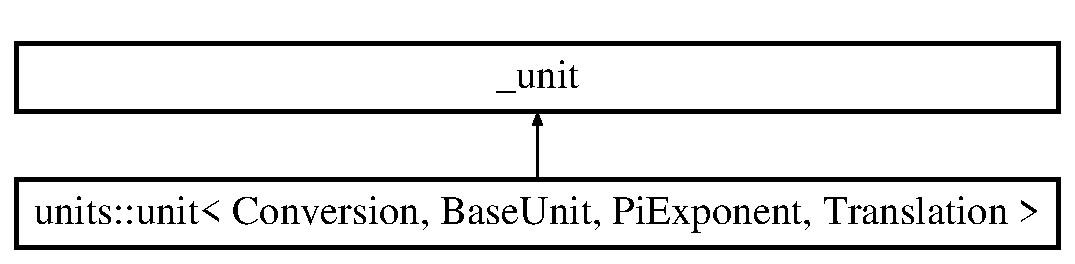
\includegraphics[height=2.000000cm]{structunits_1_1unit}
\end{center}
\end{figure}
\subsection*{Public Types}
\begin{DoxyCompactItemize}
\item 
\hypertarget{structunits_1_1unit_a04f963a5f260416cd96c9f57df5d2421}{}typedef \hyperlink{structunits_1_1traits_1_1unit__traits}{traits\+::unit\+\_\+traits}$<$ Base\+Unit $>$\+::base\+\_\+unit\+\_\+type {\bfseries base\+\_\+unit\+\_\+type}\label{structunits_1_1unit_a04f963a5f260416cd96c9f57df5d2421}

\item 
\hypertarget{structunits_1_1unit_a0f2b640f43170629369706775699fdbe}{}typedef std\+::ratio\+\_\+multiply$<$ typename Base\+Unit\+::conversion\+\_\+ratio, Conversion $>$ {\bfseries conversion\+\_\+ratio}\label{structunits_1_1unit_a0f2b640f43170629369706775699fdbe}

\item 
\hypertarget{structunits_1_1unit_aadc106afe2fedc05c154ff9f2c16025f}{}typedef std\+::ratio\+\_\+add$<$ typename Base\+Unit\+::pi\+\_\+exponent\+\_\+ratio, Pi\+Exponent $>$ {\bfseries pi\+\_\+exponent\+\_\+ratio}\label{structunits_1_1unit_aadc106afe2fedc05c154ff9f2c16025f}

\item 
\hypertarget{structunits_1_1unit_a0cdaa6959c83b6ddb1038d99a31e7814}{}typedef std\+::ratio\+\_\+add$<$ std\+::ratio\+\_\+multiply$<$ typename Base\+Unit\+::conversion\+\_\+ratio, Translation $>$, typename Base\+Unit\+::translation\+\_\+ratio $>$ {\bfseries translation\+\_\+ratio}\label{structunits_1_1unit_a0cdaa6959c83b6ddb1038d99a31e7814}

\end{DoxyCompactItemize}


\subsection{Detailed Description}
\subsubsection*{template$<$class Conversion, class Base\+Unit, class Pi\+Exponent = std\+::ratio$<$0$>$, class Translation = std\+::ratio$<$0$>$$>$struct units\+::unit$<$ Conversion, Base\+Unit, Pi\+Exponent, Translation $>$}

Type representing an arbitrary unit. 

{\ttfamily unit} types are used as tags for the {\ttfamily conversion} function. They are {\itshape not} containers (see {\ttfamily \hyperlink{classunits_1_1unit__t}{unit\+\_\+t}} for a container class). Each unit is defined by\+:


\begin{DoxyItemize}
\item A {\ttfamily std\+::ratio} defining the conversion factor to the base unit type. (e.\+g. {\ttfamily std\+::ratio$<$1,12$>$} for inches to feet)
\item A base unit that the unit is derived from (or a unit category. Must be of type {\ttfamily unit} or {\ttfamily \hyperlink{structunits_1_1base__unit}{base\+\_\+unit}})
\item An exponent representing factors of P\+I required by the conversion. (e.\+g. {\ttfamily std\+::ratio$<$-\/1$>$} for a radians to degrees conversion)
\item a ratio representing a datum translation required for the conversion (e.\+g. {\ttfamily std\+::ratio$<$32$>$} for a farenheit to celsius conversion)
\end{DoxyItemize}

Typically, a specific unit, like {\ttfamily meters}, would be implemented as a type alias of {\ttfamily unit}, i.\+e. {\ttfamily using meters = unit$<$std\+::ratio$<$1$>$, \hyperlink{namespaceunits_1_1category_a1140509fa711ad6ae98a4c001d99cfe5}{category\+::length\+\_\+unit}}, or {\ttfamily using inches = unit$<$std\+::ratio$<$1,12$>$, feet$>$}. 
\begin{DoxyTemplParams}{Template Parameters}
{\em Conversion} & std\+::ratio representing scalar multiplication factor. \\
\hline
{\em Base\+Unit} & Unit type which this unit is derived from. May be a {\ttfamily \hyperlink{structunits_1_1base__unit}{base\+\_\+unit}}, or another {\ttfamily unit}. \\
\hline
{\em Pi\+Exponent} & std\+::ratio representing the exponent of pi required by the conversion. \\
\hline
{\em Translation} & std\+::ratio representing any datum translation required by the conversion. \\
\hline
\end{DoxyTemplParams}


The documentation for this struct was generated from the following file\+:\begin{DoxyCompactItemize}
\item 
/home/nholthaus/workspace/units/include/\hyperlink{units_8h}{units.\+h}\end{DoxyCompactItemize}

\hypertarget{classunits_1_1unit__t}{}\section{units\+:\+:unit\+\_\+t$<$ Units, T, Non\+Linear\+Scale $>$ Class Template Reference}
\label{classunits_1_1unit__t}\index{units\+::unit\+\_\+t$<$ Units, T, Non\+Linear\+Scale $>$@{units\+::unit\+\_\+t$<$ Units, T, Non\+Linear\+Scale $>$}}


Container for values which represent quantities of a given unit.  




{\ttfamily \#include $<$units.\+h$>$}

Inheritance diagram for units\+:\+:unit\+\_\+t$<$ Units, T, Non\+Linear\+Scale $>$\+:\begin{figure}[H]
\begin{center}
\leavevmode
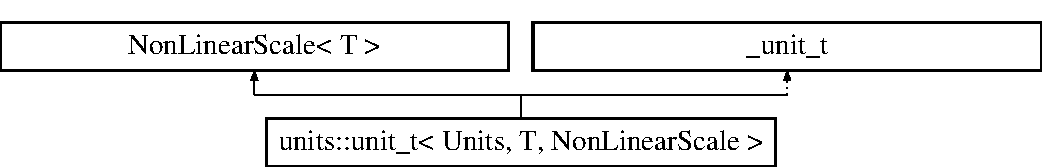
\includegraphics[height=2.000000cm]{classunits_1_1unit__t}
\end{center}
\end{figure}
\subsection*{Public Types}
\begin{DoxyCompactItemize}
\item 
\hypertarget{classunits_1_1unit__t_adb3e922bd9478c385843ee44a7607e14}{}typedef Non\+Linear\+Scale$<$ T $>$ \hyperlink{classunits_1_1unit__t_adb3e922bd9478c385843ee44a7607e14}{non\+\_\+linear\+\_\+scale\+\_\+type}\label{classunits_1_1unit__t_adb3e922bd9478c385843ee44a7607e14}

\begin{DoxyCompactList}\small\item\em Type of the non-\/linear scale of the \hyperlink{classunits_1_1unit__t}{unit\+\_\+t} (e.\+g. \hyperlink{structunits_1_1linear__scale}{linear\+\_\+scale}) \end{DoxyCompactList}\item 
\hypertarget{classunits_1_1unit__t_af3f88305faf59e0c71e8e616a2877ceb}{}typedef T \hyperlink{classunits_1_1unit__t_af3f88305faf59e0c71e8e616a2877ceb}{underlying\+\_\+type}\label{classunits_1_1unit__t_af3f88305faf59e0c71e8e616a2877ceb}

\begin{DoxyCompactList}\small\item\em Type of the underlying storage of the \hyperlink{classunits_1_1unit__t}{unit\+\_\+t} (e.\+g. double) \end{DoxyCompactList}\item 
\hypertarget{classunits_1_1unit__t_a97925b5862ffd961071a8060d0f036b3}{}typedef Units \hyperlink{classunits_1_1unit__t_a97925b5862ffd961071a8060d0f036b3}{unit\+\_\+type}\label{classunits_1_1unit__t_a97925b5862ffd961071a8060d0f036b3}

\begin{DoxyCompactList}\small\item\em Type of {\ttfamily unit} the {\ttfamily \hyperlink{classunits_1_1unit__t}{unit\+\_\+t}} represents (e.\+g. meters) \end{DoxyCompactList}\end{DoxyCompactItemize}
\subsection*{Public Member Functions}
\begin{DoxyCompactItemize}
\item 
\hypertarget{classunits_1_1unit__t_a7ec1f777253e8a5831a5bb7ad6fdb5e3}{}\hyperlink{classunits_1_1unit__t_a7ec1f777253e8a5831a5bb7ad6fdb5e3}{unit\+\_\+t} ()\label{classunits_1_1unit__t_a7ec1f777253e8a5831a5bb7ad6fdb5e3}

\begin{DoxyCompactList}\small\item\em default constructor. \end{DoxyCompactList}\item 
{\footnotesize template$<$class... Args$>$ }\\\hyperlink{classunits_1_1unit__t_a8a3086127b2fe7ae7f837e1c09ddcd5d}{unit\+\_\+t} (const Args \&...args)
\begin{DoxyCompactList}\small\item\em constructor \end{DoxyCompactList}\item 
{\footnotesize template$<$class Ty , class  = typename std\+::enable\+\_\+if$<$std\+::is\+\_\+same$<$traits\+::base\+\_\+unit\+\_\+of$<$\+Units$>$, category\+::scalar\+\_\+unit$>$\+::value \&\& std\+::is\+\_\+arithmetic$<$\+Ty$>$\+::value$>$\+::type$>$ }\\\hyperlink{classunits_1_1unit__t_a240aa805d5149ebcf2c90f72c0d6561d}{unit\+\_\+t} (Ty value)
\begin{DoxyCompactList}\small\item\em constructor \end{DoxyCompactList}\item 
{\footnotesize template$<$class Units\+Rhs , typename Ty , template$<$ typename $>$ class Nls\+Rhs$>$ }\\\hyperlink{classunits_1_1unit__t_aa50a999bfebc187549f281de23f5afe7}{unit\+\_\+t} (const \hyperlink{classunits_1_1unit__t}{unit\+\_\+t}$<$ Units\+Rhs, Ty, Nls\+Rhs $>$ \&rhs)
\begin{DoxyCompactList}\small\item\em copy constructor \end{DoxyCompactList}\item 
{\footnotesize template$<$class Units\+Rhs , typename Ty , template$<$ typename $>$ class Nls\+Rhs$>$ }\\\hyperlink{classunits_1_1unit__t}{unit\+\_\+t} \& \hyperlink{classunits_1_1unit__t_a181a9e81f77b4237eeb60be8e51de0e6}{operator=} (const \hyperlink{classunits_1_1unit__t}{unit\+\_\+t}$<$ Units\+Rhs, Ty, Nls\+Rhs $>$ \&rhs)
\begin{DoxyCompactList}\small\item\em assignment \end{DoxyCompactList}\item 
{\footnotesize template$<$class Ty , class  = typename std\+::enable\+\_\+if$<$std\+::is\+\_\+same$<$traits\+::base\+\_\+unit\+\_\+of$<$\+Units$>$, category\+::scalar\+\_\+unit$>$\+::value \&\& std\+::is\+\_\+arithmetic$<$\+Ty$>$\+::value$>$\+::type$>$ }\\\hyperlink{classunits_1_1unit__t}{unit\+\_\+t} \& \hyperlink{classunits_1_1unit__t_a8719ce4da20bef60f02bc7014fec462f}{operator=} (Ty rhs)
\begin{DoxyCompactList}\small\item\em assignment \end{DoxyCompactList}\item 
{\footnotesize template$<$class Units\+Rhs , typename Ty , template$<$ typename $>$ class Nls\+Rhs$>$ }\\bool \hyperlink{classunits_1_1unit__t_a246440e86277356cd105f9052782fc88}{operator$<$} (const \hyperlink{classunits_1_1unit__t}{unit\+\_\+t}$<$ Units\+Rhs, Ty, Nls\+Rhs $>$ \&rhs) const 
\begin{DoxyCompactList}\small\item\em less-\/than \end{DoxyCompactList}\item 
{\footnotesize template$<$class Units\+Rhs , typename Ty , template$<$ typename $>$ class Nls\+Rhs$>$ }\\bool \hyperlink{classunits_1_1unit__t_a503fdec1595b8d546eb21f8316d6cba7}{operator$<$=} (const \hyperlink{classunits_1_1unit__t}{unit\+\_\+t}$<$ Units\+Rhs, Ty, Nls\+Rhs $>$ \&rhs) const 
\begin{DoxyCompactList}\small\item\em less-\/than or equal \end{DoxyCompactList}\item 
{\footnotesize template$<$class Units\+Rhs , typename Ty , template$<$ typename $>$ class Nls\+Rhs$>$ }\\bool \hyperlink{classunits_1_1unit__t_affcb90859d439607fd1d7d95405d0e33}{operator$>$} (const \hyperlink{classunits_1_1unit__t}{unit\+\_\+t}$<$ Units\+Rhs, Ty, Nls\+Rhs $>$ \&rhs) const 
\begin{DoxyCompactList}\small\item\em greater-\/than \end{DoxyCompactList}\item 
{\footnotesize template$<$class Units\+Rhs , typename Ty , template$<$ typename $>$ class Nls\+Rhs$>$ }\\bool \hyperlink{classunits_1_1unit__t_ae3a3d9bc32509317487fa1852520420a}{operator$>$=} (const \hyperlink{classunits_1_1unit__t}{unit\+\_\+t}$<$ Units\+Rhs, Ty, Nls\+Rhs $>$ \&rhs) const 
\begin{DoxyCompactList}\small\item\em greater-\/than or equal \end{DoxyCompactList}\item 
{\footnotesize template$<$class Units\+Rhs , typename Ty , template$<$ typename $>$ class Nls\+Rhs$>$ }\\bool \hyperlink{classunits_1_1unit__t_aaa6589b34df6163f45055c9df2214629}{operator==} (const \hyperlink{classunits_1_1unit__t}{unit\+\_\+t}$<$ Units\+Rhs, Ty, Nls\+Rhs $>$ \&rhs) const 
\begin{DoxyCompactList}\small\item\em equality \end{DoxyCompactList}\item 
{\footnotesize template$<$class Units\+Rhs , typename Ty , template$<$ typename $>$ class Nls\+Rhs$>$ }\\bool \hyperlink{classunits_1_1unit__t_ab9b140f6141ea78e5304b088d6bb81b5}{operator!=} (const \hyperlink{classunits_1_1unit__t}{unit\+\_\+t}$<$ Units\+Rhs, Ty, Nls\+Rhs $>$ \&rhs) const 
\begin{DoxyCompactList}\small\item\em inequality \end{DoxyCompactList}\item 
T \hyperlink{classunits_1_1unit__t_abfc0a8abeee60499832e10f24ab5654b}{to\+Double} () const 
\begin{DoxyCompactList}\small\item\em unit value \end{DoxyCompactList}\item 
T \hyperlink{classunits_1_1unit__t_a331e19510321235c844ecb880fea6afd}{to\+Linearized\+Double} () const 
\begin{DoxyCompactList}\small\item\em linearized unit value \end{DoxyCompactList}\item 
{\footnotesize template$<$class U $>$ }\\auto \hyperlink{classunits_1_1unit__t_aea6e94679c69dafc348fd043c4d65d23}{convert} () const -\/$>$ \hyperlink{classunits_1_1unit__t}{unit\+\_\+t}$<$ U $>$
\begin{DoxyCompactList}\small\item\em conversion \end{DoxyCompactList}\item 
{\footnotesize template$<$class Ty , class  = typename std\+::enable\+\_\+if$<$std\+::is\+\_\+same$<$traits\+::base\+\_\+unit\+\_\+of$<$\+Units$>$, category\+::scalar\+\_\+unit$>$\+::value \&\& std\+::is\+\_\+arithmetic$<$\+Ty$>$\+::value$>$\+::type$>$ }\\\hyperlink{classunits_1_1unit__t_a66df18f075362a72034f14056422af4c}{operator Ty} () const 
\begin{DoxyCompactList}\small\item\em implicit type conversion. \end{DoxyCompactList}\end{DoxyCompactItemize}
\subsection*{Protected Types}
\begin{DoxyCompactItemize}
\item 
\hypertarget{classunits_1_1unit__t_ade7926dca4829a3dab64ae3c2682b491}{}using {\bfseries nls} = Non\+Linear\+Scale$<$ T $>$\label{classunits_1_1unit__t_ade7926dca4829a3dab64ae3c2682b491}

\end{DoxyCompactItemize}
\subsection*{Friends}
\begin{DoxyCompactItemize}
\item 
\hypertarget{classunits_1_1unit__t_a8d70ccbc4f5e6c787ca26bdd69eb71f5}{}{\footnotesize template$<$class U , typename Ty , template$<$ typename $>$ class Nlt$>$ }\\class {\bfseries unit\+\_\+t}\label{classunits_1_1unit__t_a8d70ccbc4f5e6c787ca26bdd69eb71f5}

\end{DoxyCompactItemize}


\subsection{Detailed Description}
\subsubsection*{template$<$class Units, typename T = double, template$<$ typename $>$ class Non\+Linear\+Scale = linear\+\_\+scale$>$class units\+::unit\+\_\+t$<$ Units, T, Non\+Linear\+Scale $>$}

Container for values which represent quantities of a given unit. 

Stores a value which represents a quantity in the given units. Unit containers (except scalar values) are {\itshape not} convertible to built-\/in c++ types, in order to provide type safety in dimensional analysis. Unit containers {\itshape are} implicitely convertible to other compatible unit container types. Unit containers support various types of arithmetic operations, depending on their scale type.

The value of a {\ttfamily \hyperlink{classunits_1_1unit__t}{unit\+\_\+t}} can only be changed on construction, or by assignment from another {\ttfamily \hyperlink{classunits_1_1unit__t}{unit\+\_\+t}} type. If necessary, the underlying value can be accessed using {\ttfamily operator()}\+:
\begin{DoxyCode}
meter\_t m(5.0);
\textcolor{keywordtype}{double} val = m(); \textcolor{comment}{// val == 5.0 }
\end{DoxyCode}
. 
\begin{DoxyTemplParams}{Template Parameters}
{\em Units} & unit tag for which type of units the {\ttfamily \hyperlink{classunits_1_1unit__t}{unit\+\_\+t}} represents (e.\+g. meters) \\
\hline
{\em T} & underlying type of the storage. Defaults to double. \\
\hline
{\em Non\+Linear\+Scale} & optional scale class for the units. Defaults to linear (i.\+e. does not scale the unit value). Examples of non-\/linear scales could be logarithmic, decibel, or richter scales. Non-\/linear scales must adhere to the non-\/linear-\/scale concept, i.\+e. {\ttfamily is\+\_\+nonlinear\+\_\+scale$<$...$>$\+::value} must be {\ttfamily true}. \\
\hline
\end{DoxyTemplParams}
\begin{DoxySeeAlso}{See also}

\begin{DoxyItemize}
\item \hyperlink{namespaceunits_1_1length_lengthContainers}{length unit containers}
\item \hyperlink{namespaceunits_1_1mass_massContainers}{mass unit containers}
\item \hyperlink{namespaceunits_1_1time_timeContainers}{time unit containers}
\item \hyperlink{namespaceunits_1_1angle_angleContainers}{angle unit containers}
\item \hyperlink{namespaceunits_1_1current_currentContainers}{current unit containers}
\item \hyperlink{namespaceunits_1_1temperature_temperatureContainers}{temperature unit containers}
\item \hyperlink{namespaceunits_1_1substance_substanceContainers}{substance unit containers}
\item \hyperlink{namespaceunits_1_1luminous__intensity_luminousIntensityContainers}{luminous intensity unit containers}
\item \hyperlink{namespaceunits_1_1solid__angle_solidAngleContainers}{solid angle unit containers}
\item \hyperlink{namespaceunits_1_1frequency_frequencyContainers}{frequency unit containers}
\item \hyperlink{namespaceunits_1_1velocity_velocityContainers}{velocity unit containers}
\item \hyperlink{namespaceunits_1_1angular__velocity_angularVelocityContainers}{angular velocity unit containers}
\item \hyperlink{namespaceunits_1_1acceleration_accelerationContainers}{acceleration unit containers}
\item \hyperlink{namespaceunits_1_1force_forceContainers}{force unit containers}
\item \hyperlink{namespaceunits_1_1pressure_pressureContainers}{pressure unit containers}
\item \hyperlink{namespaceunits_1_1charge_chargeContainers}{charge unit containers}
\item \hyperlink{namespaceunits_1_1energy_energyContainers}{energy unit containers}
\item \hyperlink{namespaceunits_1_1power_powerContainers}{power unit containers}
\item \hyperlink{namespaceunits_1_1voltage_voltageContainers}{voltage unit containers}
\item \hyperlink{namespaceunits_1_1capacitance_capacitanceContainers}{capacitance unit containers}
\item \hyperlink{namespaceunits_1_1impedance_impedanceContainers}{impedance unit containers}
\item \hyperlink{namespaceunits_1_1magnetic__flux_magneticFluxContainers}{magnetic flux unit containers}
\item \hyperlink{namespaceunits_1_1magnetic__field__strength_magneticFieldStrengthContainers}{magnetic field strength unit containers}
\item \hyperlink{namespaceunits_1_1inductance_inductanceContainers}{inductance unit containers}
\item \hyperlink{namespaceunits_1_1luminous__flux_luminousFluxContainers}{luminous flux unit containers}
\item \hyperlink{namespaceunits_1_1illuminance_illuminanceContainers}{illuminance unit containers}
\item \hyperlink{namespaceunits_1_1radiation_radiationContainers}{radiation unit containers}
\item \hyperlink{namespaceunits_1_1torque_torqueContainers}{torque unit containers}
\item \hyperlink{namespaceunits_1_1area_areaContainers}{area unit containers}
\item \hyperlink{namespaceunits_1_1volume_volumeContainers}{volume unit containers}
\item \hyperlink{namespaceunits_1_1density_densityContainers}{density unit containers}
\item \hyperlink{namespaceunits_1_1concentration_concentrationContainers}{concentration unit containers}
\item \hyperlink{namespaceunits_1_1constants_constantContainers}{constant unit containers} 
\end{DoxyItemize}
\end{DoxySeeAlso}


\subsection{Constructor \& Destructor Documentation}
\hypertarget{classunits_1_1unit__t_a8a3086127b2fe7ae7f837e1c09ddcd5d}{}\index{units\+::unit\+\_\+t@{units\+::unit\+\_\+t}!unit\+\_\+t@{unit\+\_\+t}}
\index{unit\+\_\+t@{unit\+\_\+t}!units\+::unit\+\_\+t@{units\+::unit\+\_\+t}}
\subsubsection[{unit\+\_\+t}]{\setlength{\rightskip}{0pt plus 5cm}template$<$class Units, typename T = double, template$<$ typename $>$ class Non\+Linear\+Scale = linear\+\_\+scale$>$ template$<$class... Args$>$ {\bf units\+::unit\+\_\+t}$<$ Units, T, Non\+Linear\+Scale $>$\+::{\bf unit\+\_\+t} (
\begin{DoxyParamCaption}
\item[{const Args \&...}]{args}
\end{DoxyParamCaption}
)\hspace{0.3cm}{\ttfamily [inline]}, {\ttfamily [explicit]}}\label{classunits_1_1unit__t_a8a3086127b2fe7ae7f837e1c09ddcd5d}


constructor 

constructs a new \hyperlink{classunits_1_1unit__t}{unit\+\_\+t} using the non-\/linear scale\textquotesingle{}s constructor. 
\begin{DoxyParams}[1]{Parameters}
\mbox{\tt in}  & {\em args} & constructor arguments are forwarded to the non-\/linear scale constructor. Which args are required depends on which scale is used. For the default (linear) scale, a single double-\/type value should be given. \\
\hline
\end{DoxyParams}
\hypertarget{classunits_1_1unit__t_a240aa805d5149ebcf2c90f72c0d6561d}{}\index{units\+::unit\+\_\+t@{units\+::unit\+\_\+t}!unit\+\_\+t@{unit\+\_\+t}}
\index{unit\+\_\+t@{unit\+\_\+t}!units\+::unit\+\_\+t@{units\+::unit\+\_\+t}}
\subsubsection[{unit\+\_\+t}]{\setlength{\rightskip}{0pt plus 5cm}template$<$class Units, typename T = double, template$<$ typename $>$ class Non\+Linear\+Scale = linear\+\_\+scale$>$ template$<$class Ty , class  = typename std\+::enable\+\_\+if$<$std\+::is\+\_\+same$<$traits\+::base\+\_\+unit\+\_\+of$<$\+Units$>$, category\+::scalar\+\_\+unit$>$\+::value \&\& std\+::is\+\_\+arithmetic$<$\+Ty$>$\+::value$>$\+::type$>$ {\bf units\+::unit\+\_\+t}$<$ Units, T, Non\+Linear\+Scale $>$\+::{\bf unit\+\_\+t} (
\begin{DoxyParamCaption}
\item[{Ty}]{value}
\end{DoxyParamCaption}
)\hspace{0.3cm}{\ttfamily [inline]}}\label{classunits_1_1unit__t_a240aa805d5149ebcf2c90f72c0d6561d}


constructor 

enable implicit conversions from T types O\+N\+L\+Y for linear scalar units 
\begin{DoxyParams}[1]{Parameters}
\mbox{\tt in}  & {\em value} & value of the \hyperlink{classunits_1_1unit__t}{unit\+\_\+t} \\
\hline
\end{DoxyParams}
\hypertarget{classunits_1_1unit__t_aa50a999bfebc187549f281de23f5afe7}{}\index{units\+::unit\+\_\+t@{units\+::unit\+\_\+t}!unit\+\_\+t@{unit\+\_\+t}}
\index{unit\+\_\+t@{unit\+\_\+t}!units\+::unit\+\_\+t@{units\+::unit\+\_\+t}}
\subsubsection[{unit\+\_\+t}]{\setlength{\rightskip}{0pt plus 5cm}template$<$class Units, typename T = double, template$<$ typename $>$ class Non\+Linear\+Scale = linear\+\_\+scale$>$ template$<$class Units\+Rhs , typename Ty , template$<$ typename $>$ class Nls\+Rhs$>$ {\bf units\+::unit\+\_\+t}$<$ Units, T, Non\+Linear\+Scale $>$\+::{\bf unit\+\_\+t} (
\begin{DoxyParamCaption}
\item[{const {\bf unit\+\_\+t}$<$ Units\+Rhs, Ty, Nls\+Rhs $>$ \&}]{rhs}
\end{DoxyParamCaption}
)\hspace{0.3cm}{\ttfamily [inline]}}\label{classunits_1_1unit__t_aa50a999bfebc187549f281de23f5afe7}


copy constructor 

performs implicit unit conversions if required. 
\begin{DoxyParams}[1]{Parameters}
\mbox{\tt in}  & {\em rhs} & unit to copy. \\
\hline
\end{DoxyParams}


\subsection{Member Function Documentation}
\hypertarget{classunits_1_1unit__t_aea6e94679c69dafc348fd043c4d65d23}{}\index{units\+::unit\+\_\+t@{units\+::unit\+\_\+t}!convert@{convert}}
\index{convert@{convert}!units\+::unit\+\_\+t@{units\+::unit\+\_\+t}}
\subsubsection[{convert}]{\setlength{\rightskip}{0pt plus 5cm}template$<$class Units, typename T = double, template$<$ typename $>$ class Non\+Linear\+Scale = linear\+\_\+scale$>$ template$<$class U $>$ auto {\bf units\+::unit\+\_\+t}$<$ Units, T, Non\+Linear\+Scale $>$\+::convert (
\begin{DoxyParamCaption}
{}
\end{DoxyParamCaption}
) const -\/$>$ {\bf unit\+\_\+t}$<$U$>$
		\hspace{0.3cm}{\ttfamily [inline]}}\label{classunits_1_1unit__t_aea6e94679c69dafc348fd043c4d65d23}


conversion 

Converts to a different unit container. Units can be converted to other containers implicitly, but this can be used in cases where explicit notation of a conversion is beneficial, or where an r-\/value container is needed. 
\begin{DoxyTemplParams}{Template Parameters}
{\em U} & unit (not \hyperlink{classunits_1_1unit__t}{unit\+\_\+t}) to convert to \\
\hline
\end{DoxyTemplParams}
\begin{DoxyReturn}{Returns}
a unit container with the specified units containing the equivalent value to $\ast$this. 
\end{DoxyReturn}
\hypertarget{classunits_1_1unit__t_a66df18f075362a72034f14056422af4c}{}\index{units\+::unit\+\_\+t@{units\+::unit\+\_\+t}!operator Ty@{operator Ty}}
\index{operator Ty@{operator Ty}!units\+::unit\+\_\+t@{units\+::unit\+\_\+t}}
\subsubsection[{operator Ty}]{\setlength{\rightskip}{0pt plus 5cm}template$<$class Units, typename T = double, template$<$ typename $>$ class Non\+Linear\+Scale = linear\+\_\+scale$>$ template$<$class Ty , class  = typename std\+::enable\+\_\+if$<$std\+::is\+\_\+same$<$traits\+::base\+\_\+unit\+\_\+of$<$\+Units$>$, category\+::scalar\+\_\+unit$>$\+::value \&\& std\+::is\+\_\+arithmetic$<$\+Ty$>$\+::value$>$\+::type$>$ {\bf units\+::unit\+\_\+t}$<$ Units, T, Non\+Linear\+Scale $>$\+::operator Ty (
\begin{DoxyParamCaption}
{}
\end{DoxyParamCaption}
) const\hspace{0.3cm}{\ttfamily [inline]}}\label{classunits_1_1unit__t_a66df18f075362a72034f14056422af4c}


implicit type conversion. 

only enabled for scalar unit types. \hypertarget{classunits_1_1unit__t_ab9b140f6141ea78e5304b088d6bb81b5}{}\index{units\+::unit\+\_\+t@{units\+::unit\+\_\+t}!operator"!=@{operator"!=}}
\index{operator"!=@{operator"!=}!units\+::unit\+\_\+t@{units\+::unit\+\_\+t}}
\subsubsection[{operator"!=}]{\setlength{\rightskip}{0pt plus 5cm}template$<$class Units, typename T = double, template$<$ typename $>$ class Non\+Linear\+Scale = linear\+\_\+scale$>$ template$<$class Units\+Rhs , typename Ty , template$<$ typename $>$ class Nls\+Rhs$>$ bool {\bf units\+::unit\+\_\+t}$<$ Units, T, Non\+Linear\+Scale $>$\+::operator!= (
\begin{DoxyParamCaption}
\item[{const {\bf unit\+\_\+t}$<$ Units\+Rhs, Ty, Nls\+Rhs $>$ \&}]{rhs}
\end{DoxyParamCaption}
) const\hspace{0.3cm}{\ttfamily [inline]}}\label{classunits_1_1unit__t_ab9b140f6141ea78e5304b088d6bb81b5}


inequality 

compares the linearized value of two units. Performs unit conversions if necessary. 
\begin{DoxyParams}[1]{Parameters}
\mbox{\tt in}  & {\em rhs} & right-\/hand side unit for the comparison \\
\hline
\end{DoxyParams}
\begin{DoxyReturn}{Returns}
true I\+F\+F the value of {\ttfamily this} is not equal to the value of rhs. 
\end{DoxyReturn}
\begin{DoxyNote}{Note}
This may not be suitable for all applications when the underlying\+\_\+type of \hyperlink{classunits_1_1unit__t}{unit\+\_\+t} is a double. 
\end{DoxyNote}
\hypertarget{classunits_1_1unit__t_a246440e86277356cd105f9052782fc88}{}\index{units\+::unit\+\_\+t@{units\+::unit\+\_\+t}!operator$<$@{operator$<$}}
\index{operator$<$@{operator$<$}!units\+::unit\+\_\+t@{units\+::unit\+\_\+t}}
\subsubsection[{operator$<$}]{\setlength{\rightskip}{0pt plus 5cm}template$<$class Units, typename T = double, template$<$ typename $>$ class Non\+Linear\+Scale = linear\+\_\+scale$>$ template$<$class Units\+Rhs , typename Ty , template$<$ typename $>$ class Nls\+Rhs$>$ bool {\bf units\+::unit\+\_\+t}$<$ Units, T, Non\+Linear\+Scale $>$\+::operator$<$ (
\begin{DoxyParamCaption}
\item[{const {\bf unit\+\_\+t}$<$ Units\+Rhs, Ty, Nls\+Rhs $>$ \&}]{rhs}
\end{DoxyParamCaption}
) const\hspace{0.3cm}{\ttfamily [inline]}}\label{classunits_1_1unit__t_a246440e86277356cd105f9052782fc88}


less-\/than 

compares the linearized value of two units. Performs unit conversions if necessary. 
\begin{DoxyParams}[1]{Parameters}
\mbox{\tt in}  & {\em rhs} & right-\/hand side unit for the comparison \\
\hline
\end{DoxyParams}
\begin{DoxyReturn}{Returns}
true I\+F\+F the value of {\ttfamily this} is less than the value of {\ttfamily rhs} 
\end{DoxyReturn}
\hypertarget{classunits_1_1unit__t_a503fdec1595b8d546eb21f8316d6cba7}{}\index{units\+::unit\+\_\+t@{units\+::unit\+\_\+t}!operator$<$=@{operator$<$=}}
\index{operator$<$=@{operator$<$=}!units\+::unit\+\_\+t@{units\+::unit\+\_\+t}}
\subsubsection[{operator$<$=}]{\setlength{\rightskip}{0pt plus 5cm}template$<$class Units, typename T = double, template$<$ typename $>$ class Non\+Linear\+Scale = linear\+\_\+scale$>$ template$<$class Units\+Rhs , typename Ty , template$<$ typename $>$ class Nls\+Rhs$>$ bool {\bf units\+::unit\+\_\+t}$<$ Units, T, Non\+Linear\+Scale $>$\+::operator$<$= (
\begin{DoxyParamCaption}
\item[{const {\bf unit\+\_\+t}$<$ Units\+Rhs, Ty, Nls\+Rhs $>$ \&}]{rhs}
\end{DoxyParamCaption}
) const\hspace{0.3cm}{\ttfamily [inline]}}\label{classunits_1_1unit__t_a503fdec1595b8d546eb21f8316d6cba7}


less-\/than or equal 

compares the linearized value of two units. Performs unit conversions if necessary. 
\begin{DoxyParams}[1]{Parameters}
\mbox{\tt in}  & {\em rhs} & right-\/hand side unit for the comparison \\
\hline
\end{DoxyParams}
\begin{DoxyReturn}{Returns}
true I\+F\+F the value of {\ttfamily this} is less than or equal to the value of {\ttfamily rhs} 
\end{DoxyReturn}
\hypertarget{classunits_1_1unit__t_a181a9e81f77b4237eeb60be8e51de0e6}{}\index{units\+::unit\+\_\+t@{units\+::unit\+\_\+t}!operator=@{operator=}}
\index{operator=@{operator=}!units\+::unit\+\_\+t@{units\+::unit\+\_\+t}}
\subsubsection[{operator=}]{\setlength{\rightskip}{0pt plus 5cm}template$<$class Units, typename T = double, template$<$ typename $>$ class Non\+Linear\+Scale = linear\+\_\+scale$>$ template$<$class Units\+Rhs , typename Ty , template$<$ typename $>$ class Nls\+Rhs$>$ {\bf unit\+\_\+t}\& {\bf units\+::unit\+\_\+t}$<$ Units, T, Non\+Linear\+Scale $>$\+::operator= (
\begin{DoxyParamCaption}
\item[{const {\bf unit\+\_\+t}$<$ Units\+Rhs, Ty, Nls\+Rhs $>$ \&}]{rhs}
\end{DoxyParamCaption}
)\hspace{0.3cm}{\ttfamily [inline]}}\label{classunits_1_1unit__t_a181a9e81f77b4237eeb60be8e51de0e6}


assignment 

performs implicit unit conversions if required 
\begin{DoxyParams}[1]{Parameters}
\mbox{\tt in}  & {\em rhs} & unit to copy. \\
\hline
\end{DoxyParams}
\hypertarget{classunits_1_1unit__t_a8719ce4da20bef60f02bc7014fec462f}{}\index{units\+::unit\+\_\+t@{units\+::unit\+\_\+t}!operator=@{operator=}}
\index{operator=@{operator=}!units\+::unit\+\_\+t@{units\+::unit\+\_\+t}}
\subsubsection[{operator=}]{\setlength{\rightskip}{0pt plus 5cm}template$<$class Units, typename T = double, template$<$ typename $>$ class Non\+Linear\+Scale = linear\+\_\+scale$>$ template$<$class Ty , class  = typename std\+::enable\+\_\+if$<$std\+::is\+\_\+same$<$traits\+::base\+\_\+unit\+\_\+of$<$\+Units$>$, category\+::scalar\+\_\+unit$>$\+::value \&\& std\+::is\+\_\+arithmetic$<$\+Ty$>$\+::value$>$\+::type$>$ {\bf unit\+\_\+t}\& {\bf units\+::unit\+\_\+t}$<$ Units, T, Non\+Linear\+Scale $>$\+::operator= (
\begin{DoxyParamCaption}
\item[{Ty}]{rhs}
\end{DoxyParamCaption}
)\hspace{0.3cm}{\ttfamily [inline]}}\label{classunits_1_1unit__t_a8719ce4da20bef60f02bc7014fec462f}


assignment 

performs implicit conversions from built-\/in types O\+N\+L\+Y for scalar units 
\begin{DoxyParams}[1]{Parameters}
\mbox{\tt in}  & {\em rhs} & value to copy. \\
\hline
\end{DoxyParams}
\hypertarget{classunits_1_1unit__t_aaa6589b34df6163f45055c9df2214629}{}\index{units\+::unit\+\_\+t@{units\+::unit\+\_\+t}!operator==@{operator==}}
\index{operator==@{operator==}!units\+::unit\+\_\+t@{units\+::unit\+\_\+t}}
\subsubsection[{operator==}]{\setlength{\rightskip}{0pt plus 5cm}template$<$class Units, typename T = double, template$<$ typename $>$ class Non\+Linear\+Scale = linear\+\_\+scale$>$ template$<$class Units\+Rhs , typename Ty , template$<$ typename $>$ class Nls\+Rhs$>$ bool {\bf units\+::unit\+\_\+t}$<$ Units, T, Non\+Linear\+Scale $>$\+::operator== (
\begin{DoxyParamCaption}
\item[{const {\bf unit\+\_\+t}$<$ Units\+Rhs, Ty, Nls\+Rhs $>$ \&}]{rhs}
\end{DoxyParamCaption}
) const\hspace{0.3cm}{\ttfamily [inline]}}\label{classunits_1_1unit__t_aaa6589b34df6163f45055c9df2214629}


equality 

compares the linearized value of two units. Performs unit conversions if necessary. 
\begin{DoxyParams}[1]{Parameters}
\mbox{\tt in}  & {\em rhs} & right-\/hand side unit for the comparison \\
\hline
\end{DoxyParams}
\begin{DoxyReturn}{Returns}
true I\+F\+F the value of {\ttfamily this} exactly equal to the value of rhs. 
\end{DoxyReturn}
\begin{DoxyNote}{Note}
This may not be suitable for all applications when the underlying\+\_\+type of \hyperlink{classunits_1_1unit__t}{unit\+\_\+t} is a double. 
\end{DoxyNote}
\hypertarget{classunits_1_1unit__t_affcb90859d439607fd1d7d95405d0e33}{}\index{units\+::unit\+\_\+t@{units\+::unit\+\_\+t}!operator$>$@{operator$>$}}
\index{operator$>$@{operator$>$}!units\+::unit\+\_\+t@{units\+::unit\+\_\+t}}
\subsubsection[{operator$>$}]{\setlength{\rightskip}{0pt plus 5cm}template$<$class Units, typename T = double, template$<$ typename $>$ class Non\+Linear\+Scale = linear\+\_\+scale$>$ template$<$class Units\+Rhs , typename Ty , template$<$ typename $>$ class Nls\+Rhs$>$ bool {\bf units\+::unit\+\_\+t}$<$ Units, T, Non\+Linear\+Scale $>$\+::operator$>$ (
\begin{DoxyParamCaption}
\item[{const {\bf unit\+\_\+t}$<$ Units\+Rhs, Ty, Nls\+Rhs $>$ \&}]{rhs}
\end{DoxyParamCaption}
) const\hspace{0.3cm}{\ttfamily [inline]}}\label{classunits_1_1unit__t_affcb90859d439607fd1d7d95405d0e33}


greater-\/than 

compares the linearized value of two units. Performs unit conversions if necessary. 
\begin{DoxyParams}[1]{Parameters}
\mbox{\tt in}  & {\em rhs} & right-\/hand side unit for the comparison \\
\hline
\end{DoxyParams}
\begin{DoxyReturn}{Returns}
true I\+F\+F the value of {\ttfamily this} is greater than the value of {\ttfamily rhs} 
\end{DoxyReturn}
\hypertarget{classunits_1_1unit__t_ae3a3d9bc32509317487fa1852520420a}{}\index{units\+::unit\+\_\+t@{units\+::unit\+\_\+t}!operator$>$=@{operator$>$=}}
\index{operator$>$=@{operator$>$=}!units\+::unit\+\_\+t@{units\+::unit\+\_\+t}}
\subsubsection[{operator$>$=}]{\setlength{\rightskip}{0pt plus 5cm}template$<$class Units, typename T = double, template$<$ typename $>$ class Non\+Linear\+Scale = linear\+\_\+scale$>$ template$<$class Units\+Rhs , typename Ty , template$<$ typename $>$ class Nls\+Rhs$>$ bool {\bf units\+::unit\+\_\+t}$<$ Units, T, Non\+Linear\+Scale $>$\+::operator$>$= (
\begin{DoxyParamCaption}
\item[{const {\bf unit\+\_\+t}$<$ Units\+Rhs, Ty, Nls\+Rhs $>$ \&}]{rhs}
\end{DoxyParamCaption}
) const\hspace{0.3cm}{\ttfamily [inline]}}\label{classunits_1_1unit__t_ae3a3d9bc32509317487fa1852520420a}


greater-\/than or equal 

compares the linearized value of two units. Performs unit conversions if necessary. 
\begin{DoxyParams}[1]{Parameters}
\mbox{\tt in}  & {\em rhs} & right-\/hand side unit for the comparison \\
\hline
\end{DoxyParams}
\begin{DoxyReturn}{Returns}
true I\+F\+F the value of {\ttfamily this} is greater than or equal to the value of {\ttfamily rhs} 
\end{DoxyReturn}
\hypertarget{classunits_1_1unit__t_abfc0a8abeee60499832e10f24ab5654b}{}\index{units\+::unit\+\_\+t@{units\+::unit\+\_\+t}!to\+Double@{to\+Double}}
\index{to\+Double@{to\+Double}!units\+::unit\+\_\+t@{units\+::unit\+\_\+t}}
\subsubsection[{to\+Double}]{\setlength{\rightskip}{0pt plus 5cm}template$<$class Units, typename T = double, template$<$ typename $>$ class Non\+Linear\+Scale = linear\+\_\+scale$>$ T {\bf units\+::unit\+\_\+t}$<$ Units, T, Non\+Linear\+Scale $>$\+::to\+Double (
\begin{DoxyParamCaption}
{}
\end{DoxyParamCaption}
) const\hspace{0.3cm}{\ttfamily [inline]}}\label{classunits_1_1unit__t_abfc0a8abeee60499832e10f24ab5654b}


unit value 

\begin{DoxyReturn}{Returns}
value of the unit in it\textquotesingle{}s underlying, non-\/safe type. 
\end{DoxyReturn}
\hypertarget{classunits_1_1unit__t_a331e19510321235c844ecb880fea6afd}{}\index{units\+::unit\+\_\+t@{units\+::unit\+\_\+t}!to\+Linearized\+Double@{to\+Linearized\+Double}}
\index{to\+Linearized\+Double@{to\+Linearized\+Double}!units\+::unit\+\_\+t@{units\+::unit\+\_\+t}}
\subsubsection[{to\+Linearized\+Double}]{\setlength{\rightskip}{0pt plus 5cm}template$<$class Units, typename T = double, template$<$ typename $>$ class Non\+Linear\+Scale = linear\+\_\+scale$>$ T {\bf units\+::unit\+\_\+t}$<$ Units, T, Non\+Linear\+Scale $>$\+::to\+Linearized\+Double (
\begin{DoxyParamCaption}
{}
\end{DoxyParamCaption}
) const\hspace{0.3cm}{\ttfamily [inline]}}\label{classunits_1_1unit__t_a331e19510321235c844ecb880fea6afd}


linearized unit value 

\begin{DoxyReturn}{Returns}
linearized value of unit which has a non-\/linear scale. For {\ttfamily \hyperlink{classunits_1_1unit__t}{unit\+\_\+t}} types with linear scales, this is equivalent to {\ttfamily value}. 
\end{DoxyReturn}


The documentation for this class was generated from the following file\+:\begin{DoxyCompactItemize}
\item 
/home/nholthaus/workspace/units/include/\hyperlink{units_8h}{units.\+h}\end{DoxyCompactItemize}

\hypertarget{structunits_1_1traits_1_1unit__t__traits}{}\section{units\+:\+:traits\+:\+:unit\+\_\+t\+\_\+traits$<$ T $>$ Struct Template Reference}
\label{structunits_1_1traits_1_1unit__t__traits}\index{units\+::traits\+::unit\+\_\+t\+\_\+traits$<$ T $>$@{units\+::traits\+::unit\+\_\+t\+\_\+traits$<$ T $>$}}


Trait for accessing the publically defined types of {\ttfamily \hyperlink{classunits_1_1unit__t}{units\+::unit\+\_\+t}}  




{\ttfamily \#include $<$units.\+h$>$}

\subsection*{Public Types}
\begin{DoxyCompactItemize}
\item 
\hypertarget{structunits_1_1traits_1_1unit__t__traits_a123dc73f52c3200a4eeec30b550be096}{}typedef T\+::non\+\_\+linear\+\_\+scale\+\_\+type \hyperlink{structunits_1_1traits_1_1unit__t__traits_a123dc73f52c3200a4eeec30b550be096}{non\+\_\+linear\+\_\+scale\+\_\+type}\label{structunits_1_1traits_1_1unit__t__traits_a123dc73f52c3200a4eeec30b550be096}

\begin{DoxyCompactList}\small\item\em Type of the \hyperlink{classunits_1_1unit__t}{unit\+\_\+t} non\+\_\+linear\+\_\+scale (e.\+g. \hyperlink{structunits_1_1linear__scale}{linear\+\_\+scale}, \hyperlink{structunits_1_1decibel__scale}{decibel\+\_\+scale}). This property is used to enable the proper linear or logatirhmic arithmetic functions. \end{DoxyCompactList}\item 
\hypertarget{structunits_1_1traits_1_1unit__t__traits_a67f44ead54d0f792f094a1e6eddbe51c}{}typedef T\+::underlying\+\_\+type \hyperlink{structunits_1_1traits_1_1unit__t__traits_a67f44ead54d0f792f094a1e6eddbe51c}{underlying\+\_\+type}\label{structunits_1_1traits_1_1unit__t__traits_a67f44ead54d0f792f094a1e6eddbe51c}

\begin{DoxyCompactList}\small\item\em Underlying storage type of the {\ttfamily \hyperlink{classunits_1_1unit__t}{unit\+\_\+t}}, e.\+g. {\ttfamily double}. \end{DoxyCompactList}\item 
\hypertarget{structunits_1_1traits_1_1unit__t__traits_a6de485677a031bd6051b8d4cbcfd38fb}{}typedef T\+::unit\+\_\+type \hyperlink{structunits_1_1traits_1_1unit__t__traits_a6de485677a031bd6051b8d4cbcfd38fb}{unit\+\_\+type}\label{structunits_1_1traits_1_1unit__t__traits_a6de485677a031bd6051b8d4cbcfd38fb}

\begin{DoxyCompactList}\small\item\em Type of unit the {\ttfamily \hyperlink{classunits_1_1unit__t}{unit\+\_\+t}} represents, e.\+g. {\ttfamily meters} \end{DoxyCompactList}\end{DoxyCompactItemize}


\subsection{Detailed Description}
\subsubsection*{template$<$typename T$>$struct units\+::traits\+::unit\+\_\+t\+\_\+traits$<$ T $>$}

Trait for accessing the publically defined types of {\ttfamily \hyperlink{classunits_1_1unit__t}{units\+::unit\+\_\+t}} 

The units library determines certain properties of the \hyperlink{classunits_1_1unit__t}{unit\+\_\+t} types passed to them and what they represent by using the members of the corresponding \hyperlink{structunits_1_1traits_1_1unit__t__traits}{unit\+\_\+t\+\_\+traits} instantiation. 

The documentation for this struct was generated from the following file\+:\begin{DoxyCompactItemize}
\item 
/home/nholthaus/workspace/units/include/\hyperlink{units_8h}{units.\+h}\end{DoxyCompactItemize}

\hypertarget{structunits_1_1traits_1_1unit__traits}{}\section{units\+:\+:traits\+:\+:unit\+\_\+traits$<$ T $>$ Struct Template Reference}
\label{structunits_1_1traits_1_1unit__traits}\index{units\+::traits\+::unit\+\_\+traits$<$ T $>$@{units\+::traits\+::unit\+\_\+traits$<$ T $>$}}


Traits class defining the properties of units.  




{\ttfamily \#include $<$units.\+h$>$}

\subsection*{Public Types}
\begin{DoxyCompactItemize}
\item 
\hypertarget{structunits_1_1traits_1_1unit__traits_a383a749c168d74ee16e79ec892dd2dfa}{}typedef T\+::base\+\_\+unit\+\_\+type \hyperlink{structunits_1_1traits_1_1unit__traits_a383a749c168d74ee16e79ec892dd2dfa}{base\+\_\+unit\+\_\+type}\label{structunits_1_1traits_1_1unit__traits_a383a749c168d74ee16e79ec892dd2dfa}

\begin{DoxyCompactList}\small\item\em Unit type that the unit was derived from. May be a {\ttfamily \hyperlink{structunits_1_1base__unit}{base\+\_\+unit}} or another {\ttfamily unit}. Use the {\ttfamily base\+\_\+unit\+\_\+of} trait to find the S\+I base unit type. This will be {\ttfamily void} if type {\ttfamily T} is not a unit. \end{DoxyCompactList}\item 
\hypertarget{structunits_1_1traits_1_1unit__traits_a502c916633cee73f5a5e7c6c1e654675}{}typedef T\+::conversion\+\_\+ratio \hyperlink{structunits_1_1traits_1_1unit__traits_a502c916633cee73f5a5e7c6c1e654675}{conversion\+\_\+ratio}\label{structunits_1_1traits_1_1unit__traits_a502c916633cee73f5a5e7c6c1e654675}

\begin{DoxyCompactList}\small\item\em {\ttfamily std\+::ratio} representing the conversion factor to the {\ttfamily base\+\_\+unit\+\_\+type}. This will be {\ttfamily void} if type {\ttfamily T} is not a unit. \end{DoxyCompactList}\item 
\hypertarget{structunits_1_1traits_1_1unit__traits_acf2430e728313804d63bdd1c55936967}{}typedef T\+::pi\+\_\+exponent\+\_\+ratio \hyperlink{structunits_1_1traits_1_1unit__traits_acf2430e728313804d63bdd1c55936967}{pi\+\_\+exponent\+\_\+ratio}\label{structunits_1_1traits_1_1unit__traits_acf2430e728313804d63bdd1c55936967}

\begin{DoxyCompactList}\small\item\em {\ttfamily std\+::ratio} representing the exponent of pi to be used in the conversion. This will be {\ttfamily void} if type {\ttfamily T} is not a unit. \end{DoxyCompactList}\item 
\hypertarget{structunits_1_1traits_1_1unit__traits_ab9872efa06cb637a5d6146822f7beb98}{}typedef T\+::translation\+\_\+ratio \hyperlink{structunits_1_1traits_1_1unit__traits_ab9872efa06cb637a5d6146822f7beb98}{translation\+\_\+ratio}\label{structunits_1_1traits_1_1unit__traits_ab9872efa06cb637a5d6146822f7beb98}

\begin{DoxyCompactList}\small\item\em {\ttfamily std\+::ratio} representing a datum translation to the base unit (i.\+e. degrees C to degrees F conversion). This will be {\ttfamily void} if type {\ttfamily T} is not a unit. \end{DoxyCompactList}\end{DoxyCompactItemize}


\subsection{Detailed Description}
\subsubsection*{template$<$class T$>$struct units\+::traits\+::unit\+\_\+traits$<$ T $>$}

Traits class defining the properties of units. 

The units library determines certain properties of the units passed to them and what they represent by using the members of the corresponding \hyperlink{structunits_1_1traits_1_1unit__traits}{unit\+\_\+traits} instantiation. 

The documentation for this struct was generated from the following file\+:\begin{DoxyCompactItemize}
\item 
/home/nholthaus/workspace/units/include/\hyperlink{units_8h}{units.\+h}\end{DoxyCompactItemize}

\hypertarget{structunits_1_1unit__value__add}{}\section{units\+:\+:unit\+\_\+value\+\_\+add$<$ U1, U2 $>$ Struct Template Reference}
\label{structunits_1_1unit__value__add}\index{units\+::unit\+\_\+value\+\_\+add$<$ U1, U2 $>$@{units\+::unit\+\_\+value\+\_\+add$<$ U1, U2 $>$}}


adds two \hyperlink{structunits_1_1unit__value__t}{unit\+\_\+value\+\_\+t} types at compile-\/time  




{\ttfamily \#include $<$units.\+h$>$}

Inheritance diagram for units\+:\+:unit\+\_\+value\+\_\+add$<$ U1, U2 $>$\+:\begin{figure}[H]
\begin{center}
\leavevmode
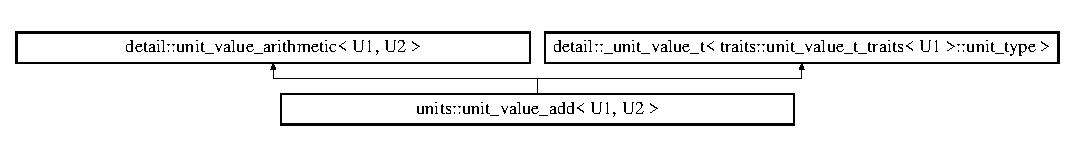
\includegraphics[height=1.450777cm]{structunits_1_1unit__value__add}
\end{center}
\end{figure}
\subsection*{Static Public Member Functions}
\begin{DoxyCompactItemize}
\item 
static const \hyperlink{classunits_1_1unit__t}{unit\+\_\+t}$<$ unit\+\_\+type $>$ \hyperlink{structunits_1_1unit__value__add_a0114743d4d923af293a9d862001b55ec}{value} ()
\begin{DoxyCompactList}\small\item\em Value of sum. \end{DoxyCompactList}\end{DoxyCompactItemize}


\subsection{Detailed Description}
\subsubsection*{template$<$class U1, class U2$>$struct units\+::unit\+\_\+value\+\_\+add$<$ U1, U2 $>$}

adds two \hyperlink{structunits_1_1unit__value__t}{unit\+\_\+value\+\_\+t} types at compile-\/time 

The resulting unit will the the {\ttfamily unit\+\_\+type} of {\ttfamily U1} 
\begin{DoxyTemplParams}{Template Parameters}
{\em U1} & left-\/hand {\ttfamily \hyperlink{structunits_1_1unit__value__t}{unit\+\_\+value\+\_\+t}} \\
\hline
{\em U2} & right-\/hand {\ttfamily \hyperlink{structunits_1_1unit__value__t}{unit\+\_\+value\+\_\+t}} \\
\hline
\end{DoxyTemplParams}
\begin{DoxySeeAlso}{See also}
unit\+\_\+value\+\_\+t\+\_\+traits to access information about the properties of the class, such as it\textquotesingle{}s \hyperlink{structunits_1_1unit}{unit} type and rational \hyperlink{structunits_1_1unit__value__add_a0114743d4d923af293a9d862001b55ec}{value}. 
\end{DoxySeeAlso}
\begin{DoxyNote}{Note}
very similar in concept to {\ttfamily std\+::ratio\+\_\+add} 
\end{DoxyNote}


\subsection{Member Function Documentation}
\hypertarget{structunits_1_1unit__value__add_a0114743d4d923af293a9d862001b55ec}{}\index{units\+::unit\+\_\+value\+\_\+add@{units\+::unit\+\_\+value\+\_\+add}!value@{value}}
\index{value@{value}!units\+::unit\+\_\+value\+\_\+add@{units\+::unit\+\_\+value\+\_\+add}}
\subsubsection[{value}]{\setlength{\rightskip}{0pt plus 5cm}template$<$class U1 , class U2 $>$ static const {\bf unit\+\_\+t}$<$unit\+\_\+type$>$ {\bf units\+::unit\+\_\+value\+\_\+add}$<$ U1, U2 $>$\+::value (
\begin{DoxyParamCaption}
{}
\end{DoxyParamCaption}
)\hspace{0.3cm}{\ttfamily [inline]}, {\ttfamily [static]}}\label{structunits_1_1unit__value__add_a0114743d4d923af293a9d862001b55ec}


Value of sum. 

Returns the calculated value of the sum of {\ttfamily U1} and {\ttfamily U2}, in the same units as {\ttfamily U1}. \begin{DoxyReturn}{Returns}
Value of the sum in the appropriate units. 
\end{DoxyReturn}


The documentation for this struct was generated from the following file\+:\begin{DoxyCompactItemize}
\item 
/home/nholthaus/workspace/units/include/\hyperlink{units_8h}{units.\+h}\end{DoxyCompactItemize}

\hypertarget{structunits_1_1unit__value__divide}{}\section{units\+:\+:unit\+\_\+value\+\_\+divide$<$ U1, U2 $>$ Struct Template Reference}
\label{structunits_1_1unit__value__divide}\index{units\+::unit\+\_\+value\+\_\+divide$<$ U1, U2 $>$@{units\+::unit\+\_\+value\+\_\+divide$<$ U1, U2 $>$}}


divides two \hyperlink{structunits_1_1unit__value__t}{unit\+\_\+value\+\_\+t} types at compile-\/time  




{\ttfamily \#include $<$units.\+h$>$}

Inheritance diagram for units\+:\+:unit\+\_\+value\+\_\+divide$<$ U1, U2 $>$\+:\begin{figure}[H]
\begin{center}
\leavevmode
\includegraphics[height=0.320733cm]{structunits_1_1unit__value__divide}
\end{center}
\end{figure}
\subsection*{Static Public Member Functions}
\begin{DoxyCompactItemize}
\item 
static const \hyperlink{classunits_1_1unit__t}{unit\+\_\+t}$<$ unit\+\_\+type $>$ \hyperlink{structunits_1_1unit__value__divide_a823b73d9ccf9df2b17fcfd96f6b1e661}{value} ()
\begin{DoxyCompactList}\small\item\em Value of quotient. \end{DoxyCompactList}\end{DoxyCompactItemize}


\subsection{Detailed Description}
\subsubsection*{template$<$class U1, class U2$>$struct units\+::unit\+\_\+value\+\_\+divide$<$ U1, U2 $>$}

divides two \hyperlink{structunits_1_1unit__value__t}{unit\+\_\+value\+\_\+t} types at compile-\/time 

The resulting unit will the the {\ttfamily unit\+\_\+type} of {\ttfamily U1} 
\begin{DoxyTemplParams}{Template Parameters}
{\em U1} & left-\/hand {\ttfamily \hyperlink{structunits_1_1unit__value__t}{unit\+\_\+value\+\_\+t}} \\
\hline
{\em U2} & right-\/hand {\ttfamily \hyperlink{structunits_1_1unit__value__t}{unit\+\_\+value\+\_\+t}} \\
\hline
\end{DoxyTemplParams}
\begin{DoxySeeAlso}{See also}
unit\+\_\+value\+\_\+t\+\_\+traits to access information about the properties of the class, such as it\textquotesingle{}s \hyperlink{structunits_1_1unit}{unit} type and rational \hyperlink{structunits_1_1unit__value__divide_a823b73d9ccf9df2b17fcfd96f6b1e661}{value}. 
\end{DoxySeeAlso}
\begin{DoxyNote}{Note}
very similar in concept to {\ttfamily std\+::ratio\+\_\+divide} 
\end{DoxyNote}


\subsection{Member Function Documentation}
\hypertarget{structunits_1_1unit__value__divide_a823b73d9ccf9df2b17fcfd96f6b1e661}{}\index{units\+::unit\+\_\+value\+\_\+divide@{units\+::unit\+\_\+value\+\_\+divide}!value@{value}}
\index{value@{value}!units\+::unit\+\_\+value\+\_\+divide@{units\+::unit\+\_\+value\+\_\+divide}}
\subsubsection[{value}]{\setlength{\rightskip}{0pt plus 5cm}template$<$class U1 , class U2 $>$ static const {\bf unit\+\_\+t}$<$unit\+\_\+type$>$ {\bf units\+::unit\+\_\+value\+\_\+divide}$<$ U1, U2 $>$\+::value (
\begin{DoxyParamCaption}
{}
\end{DoxyParamCaption}
)\hspace{0.3cm}{\ttfamily [inline]}, {\ttfamily [static]}}\label{structunits_1_1unit__value__divide_a823b73d9ccf9df2b17fcfd96f6b1e661}


Value of quotient. 

Returns the calculated value of the quotient of {\ttfamily U1} and {\ttfamily U2}, in units of {\ttfamily U1 x U2}. \begin{DoxyReturn}{Returns}
Value of the quotient in the appropriate units. 
\end{DoxyReturn}


The documentation for this struct was generated from the following file\+:\begin{DoxyCompactItemize}
\item 
/home/nholthaus/workspace/units/include/\hyperlink{units_8h}{units.\+h}\end{DoxyCompactItemize}

\hypertarget{structunits_1_1unit__value__multiply}{}\section{units\+:\+:unit\+\_\+value\+\_\+multiply$<$ U1, U2 $>$ Struct Template Reference}
\label{structunits_1_1unit__value__multiply}\index{units\+::unit\+\_\+value\+\_\+multiply$<$ U1, U2 $>$@{units\+::unit\+\_\+value\+\_\+multiply$<$ U1, U2 $>$}}


multiplies two \hyperlink{structunits_1_1unit__value__t}{unit\+\_\+value\+\_\+t} types at compile-\/time  




{\ttfamily \#include $<$units.\+h$>$}

Inheritance diagram for units\+:\+:unit\+\_\+value\+\_\+multiply$<$ U1, U2 $>$\+:\begin{figure}[H]
\begin{center}
\leavevmode
\includegraphics[height=0.284264cm]{structunits_1_1unit__value__multiply}
\end{center}
\end{figure}
\subsection*{Static Public Member Functions}
\begin{DoxyCompactItemize}
\item 
static const \hyperlink{classunits_1_1unit__t}{unit\+\_\+t}$<$ unit\+\_\+type $>$ \hyperlink{structunits_1_1unit__value__multiply_a465656e4257ea8b4d9cc5d072c45f1fe}{value} ()
\begin{DoxyCompactList}\small\item\em Value of product. \end{DoxyCompactList}\end{DoxyCompactItemize}


\subsection{Detailed Description}
\subsubsection*{template$<$class U1, class U2$>$struct units\+::unit\+\_\+value\+\_\+multiply$<$ U1, U2 $>$}

multiplies two \hyperlink{structunits_1_1unit__value__t}{unit\+\_\+value\+\_\+t} types at compile-\/time 

The resulting unit will the the {\ttfamily unit\+\_\+type} of {\ttfamily U1 $\ast$ U2} 
\begin{DoxyTemplParams}{Template Parameters}
{\em U1} & left-\/hand {\ttfamily \hyperlink{structunits_1_1unit__value__t}{unit\+\_\+value\+\_\+t}} \\
\hline
{\em U2} & right-\/hand {\ttfamily \hyperlink{structunits_1_1unit__value__t}{unit\+\_\+value\+\_\+t}} \\
\hline
\end{DoxyTemplParams}
\begin{DoxySeeAlso}{See also}
unit\+\_\+value\+\_\+t\+\_\+traits to access information about the properties of the class, such as it\textquotesingle{}s \hyperlink{structunits_1_1unit}{unit} type and rational \hyperlink{structunits_1_1unit__value__multiply_a465656e4257ea8b4d9cc5d072c45f1fe}{value}. 
\end{DoxySeeAlso}
\begin{DoxyNote}{Note}
very similar in concept to {\ttfamily std\+::ratio\+\_\+multiply} 
\end{DoxyNote}


\subsection{Member Function Documentation}
\hypertarget{structunits_1_1unit__value__multiply_a465656e4257ea8b4d9cc5d072c45f1fe}{}\index{units\+::unit\+\_\+value\+\_\+multiply@{units\+::unit\+\_\+value\+\_\+multiply}!value@{value}}
\index{value@{value}!units\+::unit\+\_\+value\+\_\+multiply@{units\+::unit\+\_\+value\+\_\+multiply}}
\subsubsection[{value}]{\setlength{\rightskip}{0pt plus 5cm}template$<$class U1 , class U2 $>$ static const {\bf unit\+\_\+t}$<$unit\+\_\+type$>$ {\bf units\+::unit\+\_\+value\+\_\+multiply}$<$ U1, U2 $>$\+::value (
\begin{DoxyParamCaption}
{}
\end{DoxyParamCaption}
)\hspace{0.3cm}{\ttfamily [inline]}, {\ttfamily [static]}}\label{structunits_1_1unit__value__multiply_a465656e4257ea8b4d9cc5d072c45f1fe}


Value of product. 

Returns the calculated value of the product of {\ttfamily U1} and {\ttfamily U2}, in units of {\ttfamily U1 x U2}. \begin{DoxyReturn}{Returns}
Value of the product in the appropriate units. 
\end{DoxyReturn}


The documentation for this struct was generated from the following file\+:\begin{DoxyCompactItemize}
\item 
/home/nholthaus/workspace/units/include/\hyperlink{units_8h}{units.\+h}\end{DoxyCompactItemize}

\hypertarget{structunits_1_1unit__value__power}{}\section{units\+:\+:unit\+\_\+value\+\_\+power$<$ U1, power $>$ Struct Template Reference}
\label{structunits_1_1unit__value__power}\index{units\+::unit\+\_\+value\+\_\+power$<$ U1, power $>$@{units\+::unit\+\_\+value\+\_\+power$<$ U1, power $>$}}


raises unit\+\_\+value\+\_\+to a power at compile-\/time  




{\ttfamily \#include $<$units.\+h$>$}

Inheritance diagram for units\+:\+:unit\+\_\+value\+\_\+power$<$ U1, power $>$\+:\begin{figure}[H]
\begin{center}
\leavevmode
\includegraphics[height=0.933333cm]{structunits_1_1unit__value__power}
\end{center}
\end{figure}
\subsection*{Static Public Member Functions}
\begin{DoxyCompactItemize}
\item 
static const \hyperlink{classunits_1_1unit__t}{unit\+\_\+t}$<$ unit\+\_\+type $>$ \hyperlink{structunits_1_1unit__value__power_a8eae2c1a34b99a111f78f57900859647}{value} ()
\begin{DoxyCompactList}\small\item\em Value of exponentiation. \end{DoxyCompactList}\end{DoxyCompactItemize}


\subsection{Detailed Description}
\subsubsection*{template$<$class U1, int power$>$struct units\+::unit\+\_\+value\+\_\+power$<$ U1, power $>$}

raises unit\+\_\+value\+\_\+to a power at compile-\/time 

The resulting unit will the {\ttfamily unit\+\_\+type} of {\ttfamily U1} squared 
\begin{DoxyTemplParams}{Template Parameters}
{\em U1} & {\ttfamily \hyperlink{structunits_1_1unit__value__t}{unit\+\_\+value\+\_\+t}} to take the exponentiation of. \\
\hline
\end{DoxyTemplParams}
\begin{DoxySeeAlso}{See also}
unit\+\_\+value\+\_\+t\+\_\+traits to access information about the properties of the class, such as it\textquotesingle{}s \hyperlink{structunits_1_1unit}{unit} type and rational \hyperlink{structunits_1_1unit__value__power_a8eae2c1a34b99a111f78f57900859647}{value}. 
\end{DoxySeeAlso}
\begin{DoxyNote}{Note}
very similar in concept to {\ttfamily \hyperlink{namespaceunits_1_1math_adf689b7864a5c78a00628574cc8dca6b}{units\+::math\+::pow}} 
\end{DoxyNote}


\subsection{Member Function Documentation}
\hypertarget{structunits_1_1unit__value__power_a8eae2c1a34b99a111f78f57900859647}{}\index{units\+::unit\+\_\+value\+\_\+power@{units\+::unit\+\_\+value\+\_\+power}!value@{value}}
\index{value@{value}!units\+::unit\+\_\+value\+\_\+power@{units\+::unit\+\_\+value\+\_\+power}}
\subsubsection[{value}]{\setlength{\rightskip}{0pt plus 5cm}template$<$class U1 , int power$>$ static const {\bf unit\+\_\+t}$<$unit\+\_\+type$>$ {\bf units\+::unit\+\_\+value\+\_\+power}$<$ U1, power $>$\+::value (
\begin{DoxyParamCaption}
{}
\end{DoxyParamCaption}
)\hspace{0.3cm}{\ttfamily [inline]}, {\ttfamily [static]}}\label{structunits_1_1unit__value__power_a8eae2c1a34b99a111f78f57900859647}


Value of exponentiation. 

Returns the calculated value of the exponentiation of {\ttfamily U1}, in units of {\ttfamily U1$^\wedge$power}. \begin{DoxyReturn}{Returns}
Value of the exponentiation in the appropriate units. 
\end{DoxyReturn}


The documentation for this struct was generated from the following file\+:\begin{DoxyCompactItemize}
\item 
/home/nholthaus/workspace/units/include/\hyperlink{units_8h}{units.\+h}\end{DoxyCompactItemize}

\hypertarget{structunits_1_1unit__value__sqrt}{}\section{units\+:\+:unit\+\_\+value\+\_\+sqrt$<$ U1, Eps $>$ Struct Template Reference}
\label{structunits_1_1unit__value__sqrt}\index{units\+::unit\+\_\+value\+\_\+sqrt$<$ U1, Eps $>$@{units\+::unit\+\_\+value\+\_\+sqrt$<$ U1, Eps $>$}}


calculates square root of \hyperlink{structunits_1_1unit__value__t}{unit\+\_\+value\+\_\+t} at compile-\/time  




{\ttfamily \#include $<$units.\+h$>$}

Inheritance diagram for units\+:\+:unit\+\_\+value\+\_\+sqrt$<$ U1, Eps $>$\+:\begin{figure}[H]
\begin{center}
\leavevmode
\includegraphics[height=1.104536cm]{structunits_1_1unit__value__sqrt}
\end{center}
\end{figure}
\subsection*{Static Public Member Functions}
\begin{DoxyCompactItemize}
\item 
static const \hyperlink{classunits_1_1unit__t}{unit\+\_\+t}$<$ unit\+\_\+type $>$ \hyperlink{structunits_1_1unit__value__sqrt_a62c14b16e45cbbf2db6b721c7aece287}{value} ()
\begin{DoxyCompactList}\small\item\em Value of square root. \end{DoxyCompactList}\end{DoxyCompactItemize}


\subsection{Detailed Description}
\subsubsection*{template$<$class U1, std\+::intmax\+\_\+t Eps = 10000000000$>$struct units\+::unit\+\_\+value\+\_\+sqrt$<$ U1, Eps $>$}

calculates square root of \hyperlink{structunits_1_1unit__value__t}{unit\+\_\+value\+\_\+t} at compile-\/time 

The resulting unit will the square root {\ttfamily unit\+\_\+type} of {\ttfamily U1} 
\begin{DoxyTemplParams}{Template Parameters}
{\em U1} & {\ttfamily \hyperlink{structunits_1_1unit__value__t}{unit\+\_\+value\+\_\+t}} to take the square root of. \\
\hline
\end{DoxyTemplParams}
\begin{DoxySeeAlso}{See also}
unit\+\_\+value\+\_\+t\+\_\+traits to access information about the properties of the class, such as it\textquotesingle{}s \hyperlink{structunits_1_1unit}{unit} type and rational \hyperlink{structunits_1_1unit__value__sqrt_a62c14b16e45cbbf2db6b721c7aece287}{value}. 
\end{DoxySeeAlso}
\begin{DoxyNote}{Note}
very similar in concept to {\ttfamily \hyperlink{group___type_traits_ga62dd90a825a801e3e29841ed51713693}{units\+::ratio\+\_\+sqrt}} 
\end{DoxyNote}


\subsection{Member Function Documentation}
\hypertarget{structunits_1_1unit__value__sqrt_a62c14b16e45cbbf2db6b721c7aece287}{}\index{units\+::unit\+\_\+value\+\_\+sqrt@{units\+::unit\+\_\+value\+\_\+sqrt}!value@{value}}
\index{value@{value}!units\+::unit\+\_\+value\+\_\+sqrt@{units\+::unit\+\_\+value\+\_\+sqrt}}
\subsubsection[{value}]{\setlength{\rightskip}{0pt plus 5cm}template$<$class U1 , std\+::intmax\+\_\+t Eps = 10000000000$>$ static const {\bf unit\+\_\+t}$<$unit\+\_\+type$>$ {\bf units\+::unit\+\_\+value\+\_\+sqrt}$<$ U1, Eps $>$\+::value (
\begin{DoxyParamCaption}
{}
\end{DoxyParamCaption}
)\hspace{0.3cm}{\ttfamily [inline]}, {\ttfamily [static]}}\label{structunits_1_1unit__value__sqrt_a62c14b16e45cbbf2db6b721c7aece287}


Value of square root. 

Returns the calculated value of the square root of {\ttfamily U1}, in units of {\ttfamily U1$^\wedge$1/2}. \begin{DoxyReturn}{Returns}
Value of the square root in the appropriate units. 
\end{DoxyReturn}


The documentation for this struct was generated from the following file\+:\begin{DoxyCompactItemize}
\item 
/home/nholthaus/workspace/units/include/\hyperlink{units_8h}{units.\+h}\end{DoxyCompactItemize}

\hypertarget{structunits_1_1unit__value__subtract}{}\section{units\+:\+:unit\+\_\+value\+\_\+subtract$<$ U1, U2 $>$ Struct Template Reference}
\label{structunits_1_1unit__value__subtract}\index{units\+::unit\+\_\+value\+\_\+subtract$<$ U1, U2 $>$@{units\+::unit\+\_\+value\+\_\+subtract$<$ U1, U2 $>$}}


subtracts two \hyperlink{structunits_1_1unit__value__t}{unit\+\_\+value\+\_\+t} types at compile-\/time  




{\ttfamily \#include $<$units.\+h$>$}

Inheritance diagram for units\+:\+:unit\+\_\+value\+\_\+subtract$<$ U1, U2 $>$\+:\begin{figure}[H]
\begin{center}
\leavevmode
\includegraphics[height=1.450777cm]{structunits_1_1unit__value__subtract}
\end{center}
\end{figure}
\subsection*{Static Public Member Functions}
\begin{DoxyCompactItemize}
\item 
static const \hyperlink{classunits_1_1unit__t}{unit\+\_\+t}$<$ unit\+\_\+type $>$ \hyperlink{structunits_1_1unit__value__subtract_abee3d3276f3fc2ee6100a8b3bcba46fe}{value} ()
\begin{DoxyCompactList}\small\item\em Value of difference. \end{DoxyCompactList}\end{DoxyCompactItemize}


\subsection{Detailed Description}
\subsubsection*{template$<$class U1, class U2$>$struct units\+::unit\+\_\+value\+\_\+subtract$<$ U1, U2 $>$}

subtracts two \hyperlink{structunits_1_1unit__value__t}{unit\+\_\+value\+\_\+t} types at compile-\/time 

The resulting unit will the the {\ttfamily unit\+\_\+type} of {\ttfamily U1} 
\begin{DoxyTemplParams}{Template Parameters}
{\em U1} & left-\/hand {\ttfamily \hyperlink{structunits_1_1unit__value__t}{unit\+\_\+value\+\_\+t}} \\
\hline
{\em U2} & right-\/hand {\ttfamily \hyperlink{structunits_1_1unit__value__t}{unit\+\_\+value\+\_\+t}} \\
\hline
\end{DoxyTemplParams}
\begin{DoxySeeAlso}{See also}
unit\+\_\+value\+\_\+t\+\_\+traits to access information about the properties of the class, such as it\textquotesingle{}s \hyperlink{structunits_1_1unit}{unit} type and rational \hyperlink{structunits_1_1unit__value__subtract_abee3d3276f3fc2ee6100a8b3bcba46fe}{value}. 
\end{DoxySeeAlso}
\begin{DoxyNote}{Note}
very similar in concept to {\ttfamily std\+::ratio\+\_\+subtract} 
\end{DoxyNote}


\subsection{Member Function Documentation}
\hypertarget{structunits_1_1unit__value__subtract_abee3d3276f3fc2ee6100a8b3bcba46fe}{}\index{units\+::unit\+\_\+value\+\_\+subtract@{units\+::unit\+\_\+value\+\_\+subtract}!value@{value}}
\index{value@{value}!units\+::unit\+\_\+value\+\_\+subtract@{units\+::unit\+\_\+value\+\_\+subtract}}
\subsubsection[{value}]{\setlength{\rightskip}{0pt plus 5cm}template$<$class U1 , class U2 $>$ static const {\bf unit\+\_\+t}$<$unit\+\_\+type$>$ {\bf units\+::unit\+\_\+value\+\_\+subtract}$<$ U1, U2 $>$\+::value (
\begin{DoxyParamCaption}
{}
\end{DoxyParamCaption}
)\hspace{0.3cm}{\ttfamily [inline]}, {\ttfamily [static]}}\label{structunits_1_1unit__value__subtract_abee3d3276f3fc2ee6100a8b3bcba46fe}


Value of difference. 

Returns the calculated value of the difference of {\ttfamily U1} and {\ttfamily U2}, in the same units as {\ttfamily U1}. \begin{DoxyReturn}{Returns}
Value of the difference in the appropriate units. 
\end{DoxyReturn}


The documentation for this struct was generated from the following file\+:\begin{DoxyCompactItemize}
\item 
/home/nholthaus/workspace/units/include/\hyperlink{units_8h}{units.\+h}\end{DoxyCompactItemize}

\hypertarget{structunits_1_1unit__value__t}{}\section{units\+:\+:unit\+\_\+value\+\_\+t$<$ Units, Num, Denom $>$ Struct Template Reference}
\label{structunits_1_1unit__value__t}\index{units\+::unit\+\_\+value\+\_\+t$<$ Units, Num, Denom $>$@{units\+::unit\+\_\+value\+\_\+t$<$ Units, Num, Denom $>$}}


Stores a rational unit value as a compile-\/time constant.  




{\ttfamily \#include $<$units.\+h$>$}

Inheritance diagram for units\+:\+:unit\+\_\+value\+\_\+t$<$ Units, Num, Denom $>$\+:\begin{figure}[H]
\begin{center}
\leavevmode
\includegraphics[height=2.000000cm]{structunits_1_1unit__value__t}
\end{center}
\end{figure}
\subsection*{Public Types}
\begin{DoxyCompactItemize}
\item 
\hypertarget{structunits_1_1unit__value__t_a075e5bcccba668f3852a25f88e13a2a7}{}typedef Units {\bfseries unit\+\_\+type}\label{structunits_1_1unit__value__t_a075e5bcccba668f3852a25f88e13a2a7}

\item 
\hypertarget{structunits_1_1unit__value__t_a3a2686045bb6ac0c42b6045fa8060fa5}{}typedef std\+::ratio$<$ Num, Denom $>$ {\bfseries ratio}\label{structunits_1_1unit__value__t_a3a2686045bb6ac0c42b6045fa8060fa5}

\end{DoxyCompactItemize}
\subsection*{Static Public Member Functions}
\begin{DoxyCompactItemize}
\item 
\hypertarget{structunits_1_1unit__value__t_ae6c20c2baf2a9509d1e1c345ec290e3a}{}static const \hyperlink{classunits_1_1unit__t}{unit\+\_\+t}$<$ Units $>$ {\bfseries value} ()\label{structunits_1_1unit__value__t_ae6c20c2baf2a9509d1e1c345ec290e3a}

\end{DoxyCompactItemize}


\subsection{Detailed Description}
\subsubsection*{template$<$typename Units, std\+::uintmax\+\_\+t Num, std\+::uintmax\+\_\+t Denom = 1$>$struct units\+::unit\+\_\+value\+\_\+t$<$ Units, Num, Denom $>$}

Stores a rational unit value as a compile-\/time constant. 

\hyperlink{structunits_1_1unit__value__t}{unit\+\_\+value\+\_\+t} is useful for performing compile-\/time arithmetic on known unit quantities. 
\begin{DoxyTemplParams}{Template Parameters}
{\em Units} & units represented by the {\ttfamily \hyperlink{structunits_1_1unit__value__t}{unit\+\_\+value\+\_\+t}} \\
\hline
{\em Num} & numerator of the represented value. \\
\hline
{\em Denom} & denominator of the represented value. \\
\hline
\end{DoxyTemplParams}
\begin{DoxySeeAlso}{See also}
unit\+\_\+value\+\_\+t\+\_\+traits to access information about the properties of the class, such as it\textquotesingle{}s \hyperlink{structunits_1_1unit}{unit} type and rational value. 
\end{DoxySeeAlso}
\begin{DoxyNote}{Note}
This is intentionally identical in concept to a {\ttfamily std\+::ratio}. 
\end{DoxyNote}


The documentation for this struct was generated from the following file\+:\begin{DoxyCompactItemize}
\item 
/home/nholthaus/workspace/units/include/\hyperlink{units_8h}{units.\+h}\end{DoxyCompactItemize}

\hypertarget{structunits_1_1traits_1_1unit__value__t__traits}{}\section{units\+:\+:traits\+:\+:unit\+\_\+value\+\_\+t\+\_\+traits$<$ T $>$ Struct Template Reference}
\label{structunits_1_1traits_1_1unit__value__t__traits}\index{units\+::traits\+::unit\+\_\+value\+\_\+t\+\_\+traits$<$ T $>$@{units\+::traits\+::unit\+\_\+value\+\_\+t\+\_\+traits$<$ T $>$}}


Trait for accessing the publically defined types of {\ttfamily units\+::unit\+\_\+value\+\_\+t\+\_\+traits}  




{\ttfamily \#include $<$units.\+h$>$}

\subsection*{Public Types}
\begin{DoxyCompactItemize}
\item 
\hypertarget{structunits_1_1traits_1_1unit__value__t__traits_a55b452f45b9191f73feda1a511376a6f}{}typedef T\+::unit\+\_\+type \hyperlink{structunits_1_1traits_1_1unit__value__t__traits_a55b452f45b9191f73feda1a511376a6f}{unit\+\_\+type}\label{structunits_1_1traits_1_1unit__value__t__traits_a55b452f45b9191f73feda1a511376a6f}

\begin{DoxyCompactList}\small\item\em Dimension represented by the {\ttfamily \hyperlink{structunits_1_1unit__value__t}{unit\+\_\+value\+\_\+t}}. \end{DoxyCompactList}\item 
\hypertarget{structunits_1_1traits_1_1unit__value__t__traits_a5de23dc20fe6d20e8255f42acce78efa}{}typedef T\+::ratio \hyperlink{structunits_1_1traits_1_1unit__value__t__traits_a5de23dc20fe6d20e8255f42acce78efa}{ratio}\label{structunits_1_1traits_1_1unit__value__t__traits_a5de23dc20fe6d20e8255f42acce78efa}

\begin{DoxyCompactList}\small\item\em Quantity represented by the {\ttfamily \hyperlink{structunits_1_1unit__value__t}{unit\+\_\+value\+\_\+t}}, expressed as arational number. \end{DoxyCompactList}\end{DoxyCompactItemize}


\subsection{Detailed Description}
\subsubsection*{template$<$typename T$>$struct units\+::traits\+::unit\+\_\+value\+\_\+t\+\_\+traits$<$ T $>$}

Trait for accessing the publically defined types of {\ttfamily units\+::unit\+\_\+value\+\_\+t\+\_\+traits} 

The units library determines certain properties of the {\ttfamily \hyperlink{structunits_1_1unit__value__t}{unit\+\_\+value\+\_\+t}} types passed to them and what they represent by using the members of the corresponding {\ttfamily \hyperlink{structunits_1_1traits_1_1unit__value__t__traits}{unit\+\_\+value\+\_\+t\+\_\+traits}} instantiation. 

The documentation for this struct was generated from the following file\+:\begin{DoxyCompactItemize}
\item 
/home/nholthaus/workspace/units/include/\hyperlink{units_8h}{units.\+h}\end{DoxyCompactItemize}

\chapter{File Documentation}
\hypertarget{units_8h}{}\section{/home/nholthaus/workspace/units/include/units.h File Reference}
\label{units_8h}\index{/home/nholthaus/workspace/units/include/units.\+h@{/home/nholthaus/workspace/units/include/units.\+h}}


Complete implementation of {\ttfamily units} -\/ a compile-\/time, header-\/only, unit conversion library built on c++14 with no dependencies.  


\subsection*{Classes}
\begin{DoxyCompactItemize}
\item 
struct \hyperlink{structunits_1_1traits_1_1is__ratio}{units\+::traits\+::is\+\_\+ratio$<$ T $>$}
\begin{DoxyCompactList}\small\item\em Trait that tests whether a type represents a std\+::ratio. \end{DoxyCompactList}\item 
struct \hyperlink{structunits_1_1traits_1_1unit__traits}{units\+::traits\+::unit\+\_\+traits$<$ T $>$}
\begin{DoxyCompactList}\small\item\em Traits class defining the properties of units. \end{DoxyCompactList}\item 
struct \hyperlink{structunits_1_1traits_1_1is__base__unit}{units\+::traits\+::is\+\_\+base\+\_\+unit$<$ T $>$}
\begin{DoxyCompactList}\small\item\em Trait which tests if a class is a {\ttfamily \hyperlink{structunits_1_1base__unit}{base\+\_\+unit}} type. \end{DoxyCompactList}\item 
struct \hyperlink{structunits_1_1traits_1_1is__unit}{units\+::traits\+::is\+\_\+unit$<$ T $>$}
\begin{DoxyCompactList}\small\item\em Traits which tests if a class is a {\ttfamily unit} \end{DoxyCompactList}\item 
struct \hyperlink{structunits_1_1base__unit}{units\+::base\+\_\+unit$<$ Meter, Kilogram, Second, Radian, Ampere, Kelvin, Mole, Candela $>$}
\begin{DoxyCompactList}\small\item\em Class representing S\+I base unit types. \end{DoxyCompactList}\item 
struct \hyperlink{structunits_1_1unit}{units\+::unit$<$ Conversion, Base\+Unit, Pi\+Exponent, Translation $>$}
\begin{DoxyCompactList}\small\item\em Type representing an arbitrary unit. \end{DoxyCompactList}\item 
struct \hyperlink{structunits_1_1traits_1_1is__convertible__unit}{units\+::traits\+::is\+\_\+convertible\+\_\+unit$<$ U1, U2 $>$}
\begin{DoxyCompactList}\small\item\em Trait which checks whether two units can be converted to each other. \end{DoxyCompactList}\item 
struct \hyperlink{structunits_1_1traits_1_1is__nonlinear__scale}{units\+::traits\+::is\+\_\+nonlinear\+\_\+scale$<$ T, Ret $>$}
\begin{DoxyCompactList}\small\item\em Trait which tests that {\ttfamily class T} meets the requirements for a non-\/linear scale. \end{DoxyCompactList}\item 
struct \hyperlink{structunits_1_1traits_1_1unit__t__traits}{units\+::traits\+::unit\+\_\+t\+\_\+traits$<$ T $>$}
\begin{DoxyCompactList}\small\item\em Trait for accessing the publically defined types of {\ttfamily \hyperlink{classunits_1_1unit__t}{units\+::unit\+\_\+t}} \end{DoxyCompactList}\item 
struct \hyperlink{structunits_1_1traits_1_1is__convertible__unit__t}{units\+::traits\+::is\+\_\+convertible\+\_\+unit\+\_\+t$<$ U1, U2 $>$}
\begin{DoxyCompactList}\small\item\em Trait which tests whether two container types derived from {\ttfamily \hyperlink{classunits_1_1unit__t}{unit\+\_\+t}} are convertible to each other. \end{DoxyCompactList}\item 
struct \hyperlink{structunits_1_1traits_1_1is__unit__t}{units\+::traits\+::is\+\_\+unit\+\_\+t$<$ T $>$}
\begin{DoxyCompactList}\small\item\em Traits which tests if a class is a {\ttfamily unit} \end{DoxyCompactList}\item 
class \hyperlink{classunits_1_1unit__t}{units\+::unit\+\_\+t$<$ Units, T, Non\+Linear\+Scale $>$}
\begin{DoxyCompactList}\small\item\em Container for values which represent quantities of a given unit. \end{DoxyCompactList}\item 
struct \hyperlink{structunits_1_1decibel__scale}{units\+::decibel\+\_\+scale$<$ T $>$}
\begin{DoxyCompactList}\small\item\em \hyperlink{classunits_1_1unit__t}{unit\+\_\+t} scale for representing decibel values. \end{DoxyCompactList}\item 
struct \hyperlink{structunits_1_1traits_1_1has__linear__scale}{units\+::traits\+::has\+\_\+linear\+\_\+scale$<$ T $>$}
\begin{DoxyCompactList}\small\item\em Trait which tests whether a type is inherited from a linear scale. \end{DoxyCompactList}\item 
struct \hyperlink{structunits_1_1traits_1_1has__decibel__scale}{units\+::traits\+::has\+\_\+decibel\+\_\+scale$<$ T $>$}
\begin{DoxyCompactList}\small\item\em Trait which tests whether a type is inherited from a decibel scale. \end{DoxyCompactList}\item 
struct \hyperlink{structunits_1_1traits_1_1is__same__scale}{units\+::traits\+::is\+\_\+same\+\_\+scale$<$ T1, T2 $>$}
\begin{DoxyCompactList}\small\item\em Trait which tests whether two types has the same non-\/linear scale. \end{DoxyCompactList}\item 
struct \hyperlink{structunits_1_1linear__scale}{units\+::linear\+\_\+scale$<$ T $>$}
\begin{DoxyCompactList}\small\item\em \hyperlink{classunits_1_1unit__t}{unit\+\_\+t} scale which is linear \end{DoxyCompactList}\item 
struct \hyperlink{structunits_1_1traits_1_1is__scalar__unit}{units\+::traits\+::is\+\_\+scalar\+\_\+unit$<$ T $>$}
\begin{DoxyCompactList}\small\item\em Trait which tests whether one or more types derived from {\ttfamily \hyperlink{classunits_1_1unit__t}{unit\+\_\+t}} represent scalar values. \end{DoxyCompactList}\item 
struct \hyperlink{structunits_1_1decibel__scale}{units\+::decibel\+\_\+scale$<$ T $>$}
\begin{DoxyCompactList}\small\item\em \hyperlink{classunits_1_1unit__t}{unit\+\_\+t} scale for representing decibel values. \end{DoxyCompactList}\item 
struct \hyperlink{structunits_1_1traits_1_1unit__value__t__traits}{units\+::traits\+::unit\+\_\+value\+\_\+t\+\_\+traits$<$ T $>$}
\begin{DoxyCompactList}\small\item\em Trait for accessing the publically defined types of {\ttfamily units\+::unit\+\_\+value\+\_\+t\+\_\+traits} \end{DoxyCompactList}\item 
struct \hyperlink{structunits_1_1unit__value__t}{units\+::unit\+\_\+value\+\_\+t$<$ Units, Num, Denom $>$}
\begin{DoxyCompactList}\small\item\em Stores a rational unit value as a compile-\/time constant. \end{DoxyCompactList}\item 
struct \hyperlink{structunits_1_1traits_1_1is__unit__value__t}{units\+::traits\+::is\+\_\+unit\+\_\+value\+\_\+t$<$ T, Units $>$}
\begin{DoxyCompactList}\small\item\em Trait which tests whether a type is a \hyperlink{structunits_1_1unit__value__t}{unit\+\_\+value\+\_\+t} representing the given unit type. \end{DoxyCompactList}\item 
struct \hyperlink{structunits_1_1traits_1_1is__unit__value__t__category}{units\+::traits\+::is\+\_\+unit\+\_\+value\+\_\+t\+\_\+category$<$ Category, T $>$}
\begin{DoxyCompactList}\small\item\em Trait which tests whether type T is a \hyperlink{structunits_1_1unit__value__t}{unit\+\_\+value\+\_\+t} with a unit type in the given category. \end{DoxyCompactList}\item 
struct \hyperlink{structunits_1_1unit__value__add}{units\+::unit\+\_\+value\+\_\+add$<$ U1, U2 $>$}
\begin{DoxyCompactList}\small\item\em adds two \hyperlink{structunits_1_1unit__value__t}{unit\+\_\+value\+\_\+t} types at compile-\/time \end{DoxyCompactList}\item 
struct \hyperlink{structunits_1_1unit__value__subtract}{units\+::unit\+\_\+value\+\_\+subtract$<$ U1, U2 $>$}
\begin{DoxyCompactList}\small\item\em subtracts two \hyperlink{structunits_1_1unit__value__t}{unit\+\_\+value\+\_\+t} types at compile-\/time \end{DoxyCompactList}\item 
struct \hyperlink{structunits_1_1unit__value__multiply}{units\+::unit\+\_\+value\+\_\+multiply$<$ U1, U2 $>$}
\begin{DoxyCompactList}\small\item\em multiplies two \hyperlink{structunits_1_1unit__value__t}{unit\+\_\+value\+\_\+t} types at compile-\/time \end{DoxyCompactList}\item 
struct \hyperlink{structunits_1_1unit__value__divide}{units\+::unit\+\_\+value\+\_\+divide$<$ U1, U2 $>$}
\begin{DoxyCompactList}\small\item\em divides two \hyperlink{structunits_1_1unit__value__t}{unit\+\_\+value\+\_\+t} types at compile-\/time \end{DoxyCompactList}\item 
struct \hyperlink{structunits_1_1unit__value__power}{units\+::unit\+\_\+value\+\_\+power$<$ U1, power $>$}
\begin{DoxyCompactList}\small\item\em raises unit\+\_\+value\+\_\+to a power at compile-\/time \end{DoxyCompactList}\item 
struct \hyperlink{structunits_1_1unit__value__sqrt}{units\+::unit\+\_\+value\+\_\+sqrt$<$ U1, Eps $>$}
\begin{DoxyCompactList}\small\item\em calculates square root of \hyperlink{structunits_1_1unit__value__t}{unit\+\_\+value\+\_\+t} at compile-\/time \end{DoxyCompactList}\item 
struct \hyperlink{structunits_1_1traits_1_1is__length__unit}{units\+::traits\+::is\+\_\+length\+\_\+unit$<$ T $>$}
\begin{DoxyCompactList}\small\item\em Trait which tests whether a type represents a unit of length. \end{DoxyCompactList}\item 
struct \hyperlink{structunits_1_1traits_1_1is__mass__unit}{units\+::traits\+::is\+\_\+mass\+\_\+unit$<$ T $>$}
\begin{DoxyCompactList}\small\item\em Trait which tests whether a type represents a unit of mass. \end{DoxyCompactList}\item 
struct \hyperlink{structunits_1_1traits_1_1is__time__unit}{units\+::traits\+::is\+\_\+time\+\_\+unit$<$ T $>$}
\begin{DoxyCompactList}\small\item\em Trait which tests whether a type represents a unit of time. \end{DoxyCompactList}\item 
struct \hyperlink{structunits_1_1traits_1_1is__angle__unit}{units\+::traits\+::is\+\_\+angle\+\_\+unit$<$ T $>$}
\begin{DoxyCompactList}\small\item\em Trait which tests whether a type represents a unit of angle. \end{DoxyCompactList}\item 
struct \hyperlink{structunits_1_1traits_1_1is__current__unit}{units\+::traits\+::is\+\_\+current\+\_\+unit$<$ T $>$}
\begin{DoxyCompactList}\small\item\em Trait which tests whether a type represents a unit of current. \end{DoxyCompactList}\item 
struct \hyperlink{structunits_1_1traits_1_1is__temperature__unit}{units\+::traits\+::is\+\_\+temperature\+\_\+unit$<$ T $>$}
\begin{DoxyCompactList}\small\item\em Trait which tests whether a type represents a unit of temperature. \end{DoxyCompactList}\item 
struct \hyperlink{structunits_1_1traits_1_1is__substance__unit}{units\+::traits\+::is\+\_\+substance\+\_\+unit$<$ T $>$}
\begin{DoxyCompactList}\small\item\em Trait which tests whether a type represents a unit of substance. \end{DoxyCompactList}\item 
struct \hyperlink{structunits_1_1traits_1_1is__luminous__intensity__unit}{units\+::traits\+::is\+\_\+luminous\+\_\+intensity\+\_\+unit$<$ T $>$}
\begin{DoxyCompactList}\small\item\em Trait which tests whether a type represents a unit of \hyperlink{namespaceunits_1_1luminous__intensity}{luminous\+\_\+intensity}. \end{DoxyCompactList}\item 
struct \hyperlink{structunits_1_1traits_1_1is__solid__angle__unit}{units\+::traits\+::is\+\_\+solid\+\_\+angle\+\_\+unit$<$ T $>$}
\begin{DoxyCompactList}\small\item\em Trait which tests whether a type represents a unit of \hyperlink{namespaceunits_1_1solid__angle}{solid\+\_\+angle}. \end{DoxyCompactList}\item 
struct \hyperlink{structunits_1_1traits_1_1is__frequency__unit}{units\+::traits\+::is\+\_\+frequency\+\_\+unit$<$ T $>$}
\begin{DoxyCompactList}\small\item\em Trait which tests whether a type represents a unit of frequency. \end{DoxyCompactList}\item 
struct \hyperlink{structunits_1_1traits_1_1is__velocity__unit}{units\+::traits\+::is\+\_\+velocity\+\_\+unit$<$ T $>$}
\begin{DoxyCompactList}\small\item\em Trait which tests whether a type represents a unit of velocity. \end{DoxyCompactList}\item 
struct \hyperlink{structunits_1_1traits_1_1is__angular__velocity__unit}{units\+::traits\+::is\+\_\+angular\+\_\+velocity\+\_\+unit$<$ T $>$}
\begin{DoxyCompactList}\small\item\em Trait which tests whether a type represents a unit of \hyperlink{namespaceunits_1_1angular__velocity}{angular\+\_\+velocity}. \end{DoxyCompactList}\item 
struct \hyperlink{structunits_1_1traits_1_1is__acceleration__unit}{units\+::traits\+::is\+\_\+acceleration\+\_\+unit$<$ T $>$}
\begin{DoxyCompactList}\small\item\em Trait which tests whether a type represents a unit of acceleration. \end{DoxyCompactList}\item 
struct \hyperlink{structunits_1_1traits_1_1is__force__unit}{units\+::traits\+::is\+\_\+force\+\_\+unit$<$ T $>$}
\begin{DoxyCompactList}\small\item\em Trait which tests whether a type represents a unit of force. \end{DoxyCompactList}\item 
struct \hyperlink{structunits_1_1traits_1_1is__pressure__unit}{units\+::traits\+::is\+\_\+pressure\+\_\+unit$<$ T $>$}
\begin{DoxyCompactList}\small\item\em Trait which tests whether a type represents a unit of pressure. \end{DoxyCompactList}\item 
struct \hyperlink{structunits_1_1traits_1_1is__charge__unit}{units\+::traits\+::is\+\_\+charge\+\_\+unit$<$ T $>$}
\begin{DoxyCompactList}\small\item\em Trait which tests whether a type represents a unit of charge. \end{DoxyCompactList}\item 
struct \hyperlink{structunits_1_1traits_1_1is__energy__unit}{units\+::traits\+::is\+\_\+energy\+\_\+unit$<$ T $>$}
\begin{DoxyCompactList}\small\item\em Trait which tests whether a type represents a unit of energy. \end{DoxyCompactList}\item 
struct \hyperlink{structunits_1_1traits_1_1is__power__unit}{units\+::traits\+::is\+\_\+power\+\_\+unit$<$ T $>$}
\begin{DoxyCompactList}\small\item\em Trait which tests whether a type represents a unit of power. \end{DoxyCompactList}\item 
struct \hyperlink{structunits_1_1traits_1_1is__voltage__unit}{units\+::traits\+::is\+\_\+voltage\+\_\+unit$<$ T $>$}
\begin{DoxyCompactList}\small\item\em Trait which tests whether a type represents a unit of voltage. \end{DoxyCompactList}\item 
struct \hyperlink{structunits_1_1traits_1_1is__capacitance__unit}{units\+::traits\+::is\+\_\+capacitance\+\_\+unit$<$ T $>$}
\begin{DoxyCompactList}\small\item\em Trait which tests whether a type represents a unit of capacitance. \end{DoxyCompactList}\item 
struct \hyperlink{structunits_1_1traits_1_1is__impedance__unit}{units\+::traits\+::is\+\_\+impedance\+\_\+unit$<$ T $>$}
\begin{DoxyCompactList}\small\item\em Trait which tests whether a type represents a unit of impedance. \end{DoxyCompactList}\item 
struct \hyperlink{structunits_1_1traits_1_1is__conductance__unit}{units\+::traits\+::is\+\_\+conductance\+\_\+unit$<$ T $>$}
\begin{DoxyCompactList}\small\item\em Trait which tests whether a type represents a unit of conductance. \end{DoxyCompactList}\item 
struct \hyperlink{structunits_1_1traits_1_1is__magnetic__flux__unit}{units\+::traits\+::is\+\_\+magnetic\+\_\+flux\+\_\+unit$<$ T $>$}
\begin{DoxyCompactList}\small\item\em Trait which tests whether a type represents a unit of \hyperlink{namespaceunits_1_1magnetic__flux}{magnetic\+\_\+flux}. \end{DoxyCompactList}\item 
struct \hyperlink{structunits_1_1traits_1_1is__magnetic__field__strength__unit}{units\+::traits\+::is\+\_\+magnetic\+\_\+field\+\_\+strength\+\_\+unit$<$ T $>$}
\begin{DoxyCompactList}\small\item\em Trait which tests whether a type represents a unit of \hyperlink{namespaceunits_1_1magnetic__field__strength}{magnetic\+\_\+field\+\_\+strength}. \end{DoxyCompactList}\item 
struct \hyperlink{structunits_1_1traits_1_1is__inductance__unit}{units\+::traits\+::is\+\_\+inductance\+\_\+unit$<$ T $>$}
\begin{DoxyCompactList}\small\item\em Trait which tests whether a type represents a unit of inductance. \end{DoxyCompactList}\item 
struct \hyperlink{structunits_1_1traits_1_1is__luminous__flux__unit}{units\+::traits\+::is\+\_\+luminous\+\_\+flux\+\_\+unit$<$ T $>$}
\begin{DoxyCompactList}\small\item\em Trait which tests whether a type represents a unit of \hyperlink{namespaceunits_1_1luminous__flux}{luminous\+\_\+flux}. \end{DoxyCompactList}\item 
struct \hyperlink{structunits_1_1traits_1_1is__illuminance__unit}{units\+::traits\+::is\+\_\+illuminance\+\_\+unit$<$ T $>$}
\begin{DoxyCompactList}\small\item\em Trait which tests whether a type represents a unit of illuminance. \end{DoxyCompactList}\item 
struct \hyperlink{structunits_1_1traits_1_1is__radioactivity__unit}{units\+::traits\+::is\+\_\+radioactivity\+\_\+unit$<$ T $>$}
\begin{DoxyCompactList}\small\item\em Trait which tests whether a type represents a unit of radiation. \end{DoxyCompactList}\item 
struct \hyperlink{structunits_1_1traits_1_1is__torque__unit}{units\+::traits\+::is\+\_\+torque\+\_\+unit$<$ T $>$}
\begin{DoxyCompactList}\small\item\em Trait which tests whether a type represents a unit of torque. \end{DoxyCompactList}\item 
struct \hyperlink{structunits_1_1traits_1_1is__area__unit}{units\+::traits\+::is\+\_\+area\+\_\+unit$<$ T $>$}
\begin{DoxyCompactList}\small\item\em Trait which tests whether a type represents a unit of area. \end{DoxyCompactList}\item 
struct \hyperlink{structunits_1_1traits_1_1is__volume__unit}{units\+::traits\+::is\+\_\+volume\+\_\+unit$<$ T $>$}
\begin{DoxyCompactList}\small\item\em Trait which tests whether a type represents a unit of volume. \end{DoxyCompactList}\item 
struct \hyperlink{structunits_1_1traits_1_1is__density__unit}{units\+::traits\+::is\+\_\+density\+\_\+unit$<$ T $>$}
\begin{DoxyCompactList}\small\item\em Trait which tests whether a type represents a unit of density. \end{DoxyCompactList}\item 
struct \hyperlink{structunits_1_1traits_1_1is__concentration__unit}{units\+::traits\+::is\+\_\+concentration\+\_\+unit$<$ T $>$}
\begin{DoxyCompactList}\small\item\em Trait which tests whether a type represents a unit of concentration. \end{DoxyCompactList}\end{DoxyCompactItemize}
\subsection*{Namespaces}
\begin{DoxyCompactItemize}
\item 
 \hyperlink{namespaceunits}{units}
\begin{DoxyCompactList}\small\item\em Unit Conversion Library namespace. \end{DoxyCompactList}\item 
 \hyperlink{namespaceunits_1_1traits}{units\+::traits}
\begin{DoxyCompactList}\small\item\em namespace representing type traits which can access the properties of types provided by the units library. \end{DoxyCompactList}\item 
 \hyperlink{namespaceunits_1_1category}{units\+::category}
\begin{DoxyCompactList}\small\item\em namespace representing the implemented base and derived unit types. \end{DoxyCompactList}\item 
 \hyperlink{namespaceunits_1_1dimensionless}{units\+::dimensionless}
\begin{DoxyCompactList}\small\item\em namespace for unit types and containers for units that have no dimension (scalar units) \end{DoxyCompactList}\item 
 \hyperlink{namespaceunits_1_1math}{units\+::math}
\begin{DoxyCompactList}\small\item\em namespace for unit-\/enabled versions of the {\ttfamily $<$cmath$>$} library \end{DoxyCompactList}\item 
 \hyperlink{namespaceunits_1_1length}{units\+::length}
\begin{DoxyCompactList}\small\item\em namespace for unit types and containers representing length values \end{DoxyCompactList}\item 
 \hyperlink{namespaceunits_1_1mass}{units\+::mass}
\begin{DoxyCompactList}\small\item\em namespace for unit types and containers representing mass values \end{DoxyCompactList}\item 
 \hyperlink{namespaceunits_1_1time}{units\+::time}
\begin{DoxyCompactList}\small\item\em namespace for unit types and containers representing time values \end{DoxyCompactList}\item 
 \hyperlink{namespaceunits_1_1angle}{units\+::angle}
\begin{DoxyCompactList}\small\item\em namespace for unit types and containers representing angle values \end{DoxyCompactList}\item 
 \hyperlink{namespaceunits_1_1current}{units\+::current}
\begin{DoxyCompactList}\small\item\em namespace for unit types and containers representing current values \end{DoxyCompactList}\item 
 \hyperlink{namespaceunits_1_1temperature}{units\+::temperature}
\begin{DoxyCompactList}\small\item\em namespace for unit types and containers representing temperature values \end{DoxyCompactList}\item 
 \hyperlink{namespaceunits_1_1substance}{units\+::substance}
\begin{DoxyCompactList}\small\item\em namespace for unit types and containers representing substance values \end{DoxyCompactList}\item 
 \hyperlink{namespaceunits_1_1luminous__intensity}{units\+::luminous\+\_\+intensity}
\begin{DoxyCompactList}\small\item\em namespace for unit types and containers representing \hyperlink{namespaceunits_1_1luminous__intensity}{luminous\+\_\+intensity} values \end{DoxyCompactList}\item 
 \hyperlink{namespaceunits_1_1solid__angle}{units\+::solid\+\_\+angle}
\begin{DoxyCompactList}\small\item\em namespace for unit types and containers representing \hyperlink{namespaceunits_1_1solid__angle}{solid\+\_\+angle} values \end{DoxyCompactList}\item 
 \hyperlink{namespaceunits_1_1frequency}{units\+::frequency}
\begin{DoxyCompactList}\small\item\em namespace for unit types and containers representing frequency values \end{DoxyCompactList}\item 
 \hyperlink{namespaceunits_1_1velocity}{units\+::velocity}
\begin{DoxyCompactList}\small\item\em namespace for unit types and containers representing velocity values \end{DoxyCompactList}\item 
 \hyperlink{namespaceunits_1_1angular__velocity}{units\+::angular\+\_\+velocity}
\begin{DoxyCompactList}\small\item\em namespace for unit types and containers representing angular velocity values \end{DoxyCompactList}\item 
 \hyperlink{namespaceunits_1_1acceleration}{units\+::acceleration}
\begin{DoxyCompactList}\small\item\em namespace for unit types and containers representing acceleration values \end{DoxyCompactList}\item 
 \hyperlink{namespaceunits_1_1force}{units\+::force}
\begin{DoxyCompactList}\small\item\em namespace for unit types and containers representing force values \end{DoxyCompactList}\item 
 \hyperlink{namespaceunits_1_1pressure}{units\+::pressure}
\begin{DoxyCompactList}\small\item\em namespace for unit types and containers representing pressure values \end{DoxyCompactList}\item 
 \hyperlink{namespaceunits_1_1charge}{units\+::charge}
\begin{DoxyCompactList}\small\item\em namespace for unit types and containers representing charge values \end{DoxyCompactList}\item 
 \hyperlink{namespaceunits_1_1energy}{units\+::energy}
\begin{DoxyCompactList}\small\item\em namespace for unit types and containers representing energy values \end{DoxyCompactList}\item 
 \hyperlink{namespaceunits_1_1power}{units\+::power}
\begin{DoxyCompactList}\small\item\em namespace for unit types and containers representing power values \end{DoxyCompactList}\item 
 \hyperlink{namespaceunits_1_1voltage}{units\+::voltage}
\begin{DoxyCompactList}\small\item\em namespace for unit types and containers representing voltage values \end{DoxyCompactList}\item 
 \hyperlink{namespaceunits_1_1capacitance}{units\+::capacitance}
\begin{DoxyCompactList}\small\item\em namespace for unit types and containers representing capacitance values \end{DoxyCompactList}\item 
 \hyperlink{namespaceunits_1_1impedance}{units\+::impedance}
\begin{DoxyCompactList}\small\item\em namespace for unit types and containers representing impedance values \end{DoxyCompactList}\item 
 \hyperlink{namespaceunits_1_1conductance}{units\+::conductance}
\begin{DoxyCompactList}\small\item\em namespace for unit types and containers representing conductance values \end{DoxyCompactList}\item 
 \hyperlink{namespaceunits_1_1magnetic__flux}{units\+::magnetic\+\_\+flux}
\begin{DoxyCompactList}\small\item\em namespace for unit types and containers representing \hyperlink{namespaceunits_1_1magnetic__flux}{magnetic\+\_\+flux} values \end{DoxyCompactList}\item 
 \hyperlink{namespaceunits_1_1magnetic__field__strength}{units\+::magnetic\+\_\+field\+\_\+strength}
\begin{DoxyCompactList}\small\item\em namespace for unit types and containers representing \hyperlink{namespaceunits_1_1magnetic__field__strength}{magnetic\+\_\+field\+\_\+strength} values \end{DoxyCompactList}\item 
 \hyperlink{namespaceunits_1_1inductance}{units\+::inductance}
\begin{DoxyCompactList}\small\item\em namespace for unit types and containers representing inductance values \end{DoxyCompactList}\item 
 \hyperlink{namespaceunits_1_1luminous__flux}{units\+::luminous\+\_\+flux}
\begin{DoxyCompactList}\small\item\em namespace for unit types and containers representing \hyperlink{namespaceunits_1_1luminous__flux}{luminous\+\_\+flux} values \end{DoxyCompactList}\item 
 \hyperlink{namespaceunits_1_1illuminance}{units\+::illuminance}
\begin{DoxyCompactList}\small\item\em namespace for unit types and containers representing illuminance values \end{DoxyCompactList}\item 
 \hyperlink{namespaceunits_1_1radiation}{units\+::radiation}
\begin{DoxyCompactList}\small\item\em namespace for unit types and containers representing radiation values \end{DoxyCompactList}\item 
 \hyperlink{namespaceunits_1_1torque}{units\+::torque}
\begin{DoxyCompactList}\small\item\em namespace for unit types and containers representing torque values \end{DoxyCompactList}\item 
 \hyperlink{namespaceunits_1_1area}{units\+::area}
\begin{DoxyCompactList}\small\item\em namespace for unit types and containers representing area values \end{DoxyCompactList}\item 
 \hyperlink{namespaceunits_1_1volume}{units\+::volume}
\begin{DoxyCompactList}\small\item\em namespace for unit types and containers representing volume values \end{DoxyCompactList}\item 
 \hyperlink{namespaceunits_1_1density}{units\+::density}
\begin{DoxyCompactList}\small\item\em namespace for unit types and containers representing density values \end{DoxyCompactList}\item 
 \hyperlink{namespaceunits_1_1concentration}{units\+::concentration}
\begin{DoxyCompactList}\small\item\em namespace for unit types and containers representing concentration values \end{DoxyCompactList}\item 
 \hyperlink{namespaceunits_1_1constants}{units\+::constants}
\begin{DoxyCompactList}\small\item\em namespace for physical constants like P\+I and Avogadro\textquotesingle{}s Number. \end{DoxyCompactList}\end{DoxyCompactItemize}
\subsection*{Typedefs}
\begin{DoxyCompactItemize}
\item 
\hypertarget{namespaceunits_1_1category_ad633be0ea9f0ebaefb2a648244a5d816}{}using \hyperlink{namespaceunits_1_1category_ad633be0ea9f0ebaefb2a648244a5d816}{units\+::category\+::scalar\+\_\+unit} = base\+\_\+unit$<$$>$\label{namespaceunits_1_1category_ad633be0ea9f0ebaefb2a648244a5d816}

\begin{DoxyCompactList}\small\item\em Represents a quantity with no dimension. \end{DoxyCompactList}\item 
\hypertarget{namespaceunits_1_1category_a70d9cdc2326b265921b36493485b1254}{}using \hyperlink{namespaceunits_1_1category_a70d9cdc2326b265921b36493485b1254}{units\+::category\+::dimensionless\+\_\+unit} = base\+\_\+unit$<$$>$\label{namespaceunits_1_1category_a70d9cdc2326b265921b36493485b1254}

\begin{DoxyCompactList}\small\item\em Represents a quantity with no dimension. \end{DoxyCompactList}\item 
\hypertarget{namespaceunits_1_1category_a1140509fa711ad6ae98a4c001d99cfe5}{}using \hyperlink{namespaceunits_1_1category_a1140509fa711ad6ae98a4c001d99cfe5}{units\+::category\+::length\+\_\+unit} = base\+\_\+unit$<$ std\+::ratio$<$ 1 $>$$>$\label{namespaceunits_1_1category_a1140509fa711ad6ae98a4c001d99cfe5}

\begin{DoxyCompactList}\small\item\em Represents an S\+I base unit of length. \end{DoxyCompactList}\item 
\hypertarget{namespaceunits_1_1category_a2a957f5535dc0cbe3d3fb3f31e5f0d21}{}using \hyperlink{namespaceunits_1_1category_a2a957f5535dc0cbe3d3fb3f31e5f0d21}{units\+::category\+::mass\+\_\+unit} = base\+\_\+unit$<$ std\+::ratio$<$ 0 $>$, std\+::ratio$<$ 1 $>$$>$\label{namespaceunits_1_1category_a2a957f5535dc0cbe3d3fb3f31e5f0d21}

\begin{DoxyCompactList}\small\item\em Represents an S\+I base unit of mass. \end{DoxyCompactList}\item 
\hypertarget{namespaceunits_1_1category_a505444228cdf173b75aeed6932d7e1a9}{}using \hyperlink{namespaceunits_1_1category_a505444228cdf173b75aeed6932d7e1a9}{units\+::category\+::time\+\_\+unit} = base\+\_\+unit$<$ std\+::ratio$<$ 0 $>$, std\+::ratio$<$ 0 $>$, std\+::ratio$<$ 1 $>$$>$\label{namespaceunits_1_1category_a505444228cdf173b75aeed6932d7e1a9}

\begin{DoxyCompactList}\small\item\em Represents an S\+I base unit of time. \end{DoxyCompactList}\item 
\hypertarget{namespaceunits_1_1category_a7f431fefc267dd924d23fe6f3c7db3d1}{}using \hyperlink{namespaceunits_1_1category_a7f431fefc267dd924d23fe6f3c7db3d1}{units\+::category\+::angle\+\_\+unit} = base\+\_\+unit$<$ std\+::ratio$<$ 0 $>$, std\+::ratio$<$ 0 $>$, std\+::ratio$<$ 0 $>$, std\+::ratio$<$ 1 $>$$>$\label{namespaceunits_1_1category_a7f431fefc267dd924d23fe6f3c7db3d1}

\begin{DoxyCompactList}\small\item\em Represents an S\+I base unit of angle. \end{DoxyCompactList}\item 
\hypertarget{namespaceunits_1_1category_af018d7d3f53e57d660b51d77c5e7a437}{}using \hyperlink{namespaceunits_1_1category_af018d7d3f53e57d660b51d77c5e7a437}{units\+::category\+::current\+\_\+unit} = base\+\_\+unit$<$ std\+::ratio$<$ 0 $>$, std\+::ratio$<$ 0 $>$, std\+::ratio$<$ 0 $>$, std\+::ratio$<$ 0 $>$, std\+::ratio$<$ 1 $>$$>$\label{namespaceunits_1_1category_af018d7d3f53e57d660b51d77c5e7a437}

\begin{DoxyCompactList}\small\item\em Represents an S\+I base unit of current. \end{DoxyCompactList}\item 
\hypertarget{namespaceunits_1_1category_a3132de15d76bba5313de2ed97f8cf950}{}using \hyperlink{namespaceunits_1_1category_a3132de15d76bba5313de2ed97f8cf950}{units\+::category\+::temperature\+\_\+unit} = base\+\_\+unit$<$ std\+::ratio$<$ 0 $>$, std\+::ratio$<$ 0 $>$, std\+::ratio$<$ 0 $>$, std\+::ratio$<$ 0 $>$, std\+::ratio$<$ 0 $>$, std\+::ratio$<$ 1 $>$$>$\label{namespaceunits_1_1category_a3132de15d76bba5313de2ed97f8cf950}

\begin{DoxyCompactList}\small\item\em Represents an S\+I base unit of temperature. \end{DoxyCompactList}\item 
\hypertarget{namespaceunits_1_1category_a9603923620ee542573e69d4d16c0ce3e}{}using \hyperlink{namespaceunits_1_1category_a9603923620ee542573e69d4d16c0ce3e}{units\+::category\+::substance\+\_\+unit} = base\+\_\+unit$<$ std\+::ratio$<$ 0 $>$, std\+::ratio$<$ 0 $>$, std\+::ratio$<$ 0 $>$, std\+::ratio$<$ 0 $>$, std\+::ratio$<$ 0 $>$, std\+::ratio$<$ 0 $>$, std\+::ratio$<$ 1 $>$$>$\label{namespaceunits_1_1category_a9603923620ee542573e69d4d16c0ce3e}

\begin{DoxyCompactList}\small\item\em Represents an S\+I base unit of amount of substance. \end{DoxyCompactList}\item 
\hypertarget{namespaceunits_1_1category_a5a594dba761bc49d85a99a9a03b5f638}{}using \hyperlink{namespaceunits_1_1category_a5a594dba761bc49d85a99a9a03b5f638}{units\+::category\+::luminous\+\_\+intensity\+\_\+unit} = base\+\_\+unit$<$ std\+::ratio$<$ 0 $>$, std\+::ratio$<$ 0 $>$, std\+::ratio$<$ 0 $>$, std\+::ratio$<$ 0 $>$, std\+::ratio$<$ 0 $>$, std\+::ratio$<$ 0 $>$, std\+::ratio$<$ 0 $>$, std\+::ratio$<$ 1 $>$$>$\label{namespaceunits_1_1category_a5a594dba761bc49d85a99a9a03b5f638}

\begin{DoxyCompactList}\small\item\em Represents an S\+I base unit of luminous intensity. \end{DoxyCompactList}\item 
\hypertarget{namespaceunits_1_1category_ac288b5181dd5ed221d8d070b5d36137d}{}using \hyperlink{namespaceunits_1_1category_ac288b5181dd5ed221d8d070b5d36137d}{units\+::category\+::solid\+\_\+angle\+\_\+unit} = base\+\_\+unit$<$ std\+::ratio$<$ 0 $>$, std\+::ratio$<$ 0 $>$, std\+::ratio$<$ 0 $>$, std\+::ratio$<$ 2 $>$, std\+::ratio$<$ 0 $>$, std\+::ratio$<$ 0 $>$, std\+::ratio$<$ 0 $>$, std\+::ratio$<$ 0 $>$$>$\label{namespaceunits_1_1category_ac288b5181dd5ed221d8d070b5d36137d}

\begin{DoxyCompactList}\small\item\em Represents an S\+I derived unit of solid angle. \end{DoxyCompactList}\item 
\hypertarget{namespaceunits_1_1category_a5abfda6ffc83788eaab44d80e1acadda}{}using \hyperlink{namespaceunits_1_1category_a5abfda6ffc83788eaab44d80e1acadda}{units\+::category\+::frequency\+\_\+unit} = base\+\_\+unit$<$ std\+::ratio$<$ 0 $>$, std\+::ratio$<$ 0 $>$, std\+::ratio$<$-\/1 $>$$>$\label{namespaceunits_1_1category_a5abfda6ffc83788eaab44d80e1acadda}

\begin{DoxyCompactList}\small\item\em Represents an S\+I derived unit of frequency. \end{DoxyCompactList}\item 
\hypertarget{namespaceunits_1_1category_a47c81b9d092be905b13720353ac1d994}{}using \hyperlink{namespaceunits_1_1category_a47c81b9d092be905b13720353ac1d994}{units\+::category\+::velocity\+\_\+unit} = base\+\_\+unit$<$ std\+::ratio$<$ 1 $>$, std\+::ratio$<$ 0 $>$, std\+::ratio$<$-\/1 $>$$>$\label{namespaceunits_1_1category_a47c81b9d092be905b13720353ac1d994}

\begin{DoxyCompactList}\small\item\em Represents an S\+I derived unit of velocity. \end{DoxyCompactList}\item 
\hypertarget{namespaceunits_1_1category_acb7b5604c20499976d9eeb13d2871536}{}using \hyperlink{namespaceunits_1_1category_acb7b5604c20499976d9eeb13d2871536}{units\+::category\+::angular\+\_\+velocity\+\_\+unit} = base\+\_\+unit$<$ std\+::ratio$<$ 0 $>$, std\+::ratio$<$ 0 $>$, std\+::ratio$<$-\/1 $>$, std\+::ratio$<$ 1 $>$$>$\label{namespaceunits_1_1category_acb7b5604c20499976d9eeb13d2871536}

\begin{DoxyCompactList}\small\item\em Represents an S\+I derived unit of angular velocity. \end{DoxyCompactList}\item 
\hypertarget{namespaceunits_1_1category_a176b75b1e0ac2ee900d9c21704cd041e}{}using \hyperlink{namespaceunits_1_1category_a176b75b1e0ac2ee900d9c21704cd041e}{units\+::category\+::acceleration\+\_\+unit} = base\+\_\+unit$<$ std\+::ratio$<$ 1 $>$, std\+::ratio$<$ 0 $>$, std\+::ratio$<$-\/2 $>$$>$\label{namespaceunits_1_1category_a176b75b1e0ac2ee900d9c21704cd041e}

\begin{DoxyCompactList}\small\item\em Represents an S\+I derived unit of acceleration. \end{DoxyCompactList}\item 
\hypertarget{namespaceunits_1_1category_aac6f93abf7809deaddcec0f6edec7cc3}{}using \hyperlink{namespaceunits_1_1category_aac6f93abf7809deaddcec0f6edec7cc3}{units\+::category\+::force\+\_\+unit} = base\+\_\+unit$<$ std\+::ratio$<$ 1 $>$, std\+::ratio$<$ 1 $>$, std\+::ratio$<$-\/2 $>$$>$\label{namespaceunits_1_1category_aac6f93abf7809deaddcec0f6edec7cc3}

\begin{DoxyCompactList}\small\item\em Represents an S\+I derived unit of force. \end{DoxyCompactList}\item 
\hypertarget{namespaceunits_1_1category_adf9fa681139dac718dc7455ca2d5e11f}{}using \hyperlink{namespaceunits_1_1category_adf9fa681139dac718dc7455ca2d5e11f}{units\+::category\+::pressure\+\_\+unit} = base\+\_\+unit$<$ std\+::ratio$<$-\/1 $>$, std\+::ratio$<$ 1 $>$, std\+::ratio$<$-\/2 $>$$>$\label{namespaceunits_1_1category_adf9fa681139dac718dc7455ca2d5e11f}

\begin{DoxyCompactList}\small\item\em Represents an S\+I derived unit of pressure. \end{DoxyCompactList}\item 
\hypertarget{namespaceunits_1_1category_a2402ebbd5f61c597bf6120629a2582e7}{}using \hyperlink{namespaceunits_1_1category_a2402ebbd5f61c597bf6120629a2582e7}{units\+::category\+::charge\+\_\+unit} = base\+\_\+unit$<$ std\+::ratio$<$ 0 $>$, std\+::ratio$<$ 0 $>$, std\+::ratio$<$ 1 $>$, std\+::ratio$<$ 0 $>$, std\+::ratio$<$ 1 $>$$>$\label{namespaceunits_1_1category_a2402ebbd5f61c597bf6120629a2582e7}

\begin{DoxyCompactList}\small\item\em Represents an S\+I derived unit of charge. \end{DoxyCompactList}\item 
\hypertarget{namespaceunits_1_1category_a20ac4baa3d6500112b49b00ef502aba1}{}using \hyperlink{namespaceunits_1_1category_a20ac4baa3d6500112b49b00ef502aba1}{units\+::category\+::energy\+\_\+unit} = base\+\_\+unit$<$ std\+::ratio$<$ 2 $>$, std\+::ratio$<$ 1 $>$, std\+::ratio$<$-\/2 $>$$>$\label{namespaceunits_1_1category_a20ac4baa3d6500112b49b00ef502aba1}

\begin{DoxyCompactList}\small\item\em Represents an S\+I derived unit of energy. \end{DoxyCompactList}\item 
\hypertarget{namespaceunits_1_1category_aa595eeccb878cce2d88a3509aab0b2a6}{}using \hyperlink{namespaceunits_1_1category_aa595eeccb878cce2d88a3509aab0b2a6}{units\+::category\+::power\+\_\+unit} = base\+\_\+unit$<$ std\+::ratio$<$ 2 $>$, std\+::ratio$<$ 1 $>$, std\+::ratio$<$-\/3 $>$$>$\label{namespaceunits_1_1category_aa595eeccb878cce2d88a3509aab0b2a6}

\begin{DoxyCompactList}\small\item\em Represents an S\+I derived unit of power. \end{DoxyCompactList}\item 
\hypertarget{namespaceunits_1_1category_aaac5d18aab461c59602bf8f07861d26e}{}using \hyperlink{namespaceunits_1_1category_aaac5d18aab461c59602bf8f07861d26e}{units\+::category\+::voltage\+\_\+unit} = base\+\_\+unit$<$ std\+::ratio$<$ 2 $>$, std\+::ratio$<$ 1 $>$, std\+::ratio$<$-\/3 $>$, std\+::ratio$<$ 0 $>$, std\+::ratio$<$-\/1 $>$$>$\label{namespaceunits_1_1category_aaac5d18aab461c59602bf8f07861d26e}

\begin{DoxyCompactList}\small\item\em Represents an S\+I derived unit of voltage. \end{DoxyCompactList}\item 
\hypertarget{namespaceunits_1_1category_a0485a4663b435d78582744b8b83ea3c2}{}using \hyperlink{namespaceunits_1_1category_a0485a4663b435d78582744b8b83ea3c2}{units\+::category\+::capacitance\+\_\+unit} = base\+\_\+unit$<$ std\+::ratio$<$-\/2 $>$, std\+::ratio$<$-\/1 $>$, std\+::ratio$<$ 4 $>$, std\+::ratio$<$ 0 $>$, std\+::ratio$<$ 2 $>$$>$\label{namespaceunits_1_1category_a0485a4663b435d78582744b8b83ea3c2}

\begin{DoxyCompactList}\small\item\em Represents an S\+I derived unit of capacitance. \end{DoxyCompactList}\item 
\hypertarget{namespaceunits_1_1category_a0b9fe7547ad43633e885a8b3c8201840}{}using \hyperlink{namespaceunits_1_1category_a0b9fe7547ad43633e885a8b3c8201840}{units\+::category\+::impedance\+\_\+unit} = base\+\_\+unit$<$ std\+::ratio$<$ 2 $>$, std\+::ratio$<$ 1 $>$, std\+::ratio$<$-\/3 $>$, std\+::ratio$<$ 0 $>$, std\+::ratio$<$-\/2 $>$$>$\label{namespaceunits_1_1category_a0b9fe7547ad43633e885a8b3c8201840}

\begin{DoxyCompactList}\small\item\em Represents an S\+I derived unit of impedance. \end{DoxyCompactList}\item 
\hypertarget{namespaceunits_1_1category_a15b4c4ec156dfa3f11f5123389182e4e}{}using \hyperlink{namespaceunits_1_1category_a15b4c4ec156dfa3f11f5123389182e4e}{units\+::category\+::conductance\+\_\+unit} = base\+\_\+unit$<$ std\+::ratio$<$-\/2 $>$, std\+::ratio$<$-\/1 $>$, std\+::ratio$<$ 3 $>$, std\+::ratio$<$ 0 $>$, std\+::ratio$<$ 2 $>$$>$\label{namespaceunits_1_1category_a15b4c4ec156dfa3f11f5123389182e4e}

\begin{DoxyCompactList}\small\item\em Represents an S\+I derived unit of conductance. \end{DoxyCompactList}\item 
\hypertarget{namespaceunits_1_1category_a869ab7acbc230b4c7bc8df74619d2eaa}{}using \hyperlink{namespaceunits_1_1category_a869ab7acbc230b4c7bc8df74619d2eaa}{units\+::category\+::magnetic\+\_\+flux\+\_\+unit} = base\+\_\+unit$<$ std\+::ratio$<$ 2 $>$, std\+::ratio$<$ 1 $>$, std\+::ratio$<$-\/2 $>$, std\+::ratio$<$ 0 $>$, std\+::ratio$<$-\/1 $>$$>$\label{namespaceunits_1_1category_a869ab7acbc230b4c7bc8df74619d2eaa}

\begin{DoxyCompactList}\small\item\em Represents an S\+I derived unit of magnetic flux. \end{DoxyCompactList}\item 
\hypertarget{namespaceunits_1_1category_aac428848b9d8c5e6b21457f61096676a}{}using \hyperlink{namespaceunits_1_1category_aac428848b9d8c5e6b21457f61096676a}{units\+::category\+::magnetic\+\_\+field\+\_\+strength\+\_\+unit} = base\+\_\+unit$<$ std\+::ratio$<$ 0 $>$, std\+::ratio$<$ 1 $>$, std\+::ratio$<$-\/2 $>$, std\+::ratio$<$ 0 $>$, std\+::ratio$<$-\/1 $>$$>$\label{namespaceunits_1_1category_aac428848b9d8c5e6b21457f61096676a}

\begin{DoxyCompactList}\small\item\em Represents an S\+I derived unit of magnetic field strength. \end{DoxyCompactList}\item 
\hypertarget{namespaceunits_1_1category_ad0714439849450c6ad18b82777cb3884}{}using \hyperlink{namespaceunits_1_1category_ad0714439849450c6ad18b82777cb3884}{units\+::category\+::inductance\+\_\+unit} = base\+\_\+unit$<$ std\+::ratio$<$ 2 $>$, std\+::ratio$<$ 1 $>$, std\+::ratio$<$-\/2 $>$, std\+::ratio$<$ 0 $>$, std\+::ratio$<$-\/2 $>$$>$\label{namespaceunits_1_1category_ad0714439849450c6ad18b82777cb3884}

\begin{DoxyCompactList}\small\item\em Represents an S\+I derived unit of inductance. \end{DoxyCompactList}\item 
\hypertarget{namespaceunits_1_1category_ad6cd329153c512e1aa33f56812660177}{}using \hyperlink{namespaceunits_1_1category_ad6cd329153c512e1aa33f56812660177}{units\+::category\+::luminous\+\_\+flux\+\_\+unit} = base\+\_\+unit$<$ std\+::ratio$<$ 0 $>$, std\+::ratio$<$ 0 $>$, std\+::ratio$<$ 0 $>$, std\+::ratio$<$ 2 $>$, std\+::ratio$<$ 0 $>$, std\+::ratio$<$ 0 $>$, std\+::ratio$<$ 0 $>$, std\+::ratio$<$ 1 $>$$>$\label{namespaceunits_1_1category_ad6cd329153c512e1aa33f56812660177}

\begin{DoxyCompactList}\small\item\em Represents an S\+I derived unit of luminous flux. \end{DoxyCompactList}\item 
\hypertarget{namespaceunits_1_1category_aaec672317a59eeaeac88c0be6bcea12c}{}using \hyperlink{namespaceunits_1_1category_aaec672317a59eeaeac88c0be6bcea12c}{units\+::category\+::illuminance\+\_\+unit} = base\+\_\+unit$<$ std\+::ratio$<$-\/2 $>$, std\+::ratio$<$ 0 $>$, std\+::ratio$<$ 0 $>$, std\+::ratio$<$ 2 $>$, std\+::ratio$<$ 0 $>$, std\+::ratio$<$ 0 $>$, std\+::ratio$<$ 0 $>$, std\+::ratio$<$ 1 $>$$>$\label{namespaceunits_1_1category_aaec672317a59eeaeac88c0be6bcea12c}

\begin{DoxyCompactList}\small\item\em Represents an S\+I derived unit of illuminance. \end{DoxyCompactList}\item 
\hypertarget{namespaceunits_1_1category_a0ce14d5661fcd514f6160000c1b3ac2a}{}using \hyperlink{namespaceunits_1_1category_a0ce14d5661fcd514f6160000c1b3ac2a}{units\+::category\+::radioactivity\+\_\+unit} = base\+\_\+unit$<$ std\+::ratio$<$ 0 $>$, std\+::ratio$<$ 0 $>$, std\+::ratio$<$-\/1 $>$$>$\label{namespaceunits_1_1category_a0ce14d5661fcd514f6160000c1b3ac2a}

\begin{DoxyCompactList}\small\item\em Represents an S\+I derived unit of radioactivity. \end{DoxyCompactList}\item 
\hypertarget{namespaceunits_1_1category_a751792d53b9d7b10e926c65f0e0e2980}{}using \hyperlink{namespaceunits_1_1category_a751792d53b9d7b10e926c65f0e0e2980}{units\+::category\+::torque\+\_\+unit} = base\+\_\+unit$<$ std\+::ratio$<$ 2 $>$, std\+::ratio$<$ 1 $>$, std\+::ratio$<$-\/2 $>$$>$\label{namespaceunits_1_1category_a751792d53b9d7b10e926c65f0e0e2980}

\begin{DoxyCompactList}\small\item\em Represents an S\+I derived unit of torque. \end{DoxyCompactList}\item 
\hypertarget{namespaceunits_1_1category_af6be136b7d9c842cb68b24eac22e79d1}{}using \hyperlink{namespaceunits_1_1category_af6be136b7d9c842cb68b24eac22e79d1}{units\+::category\+::area\+\_\+unit} = base\+\_\+unit$<$ std\+::ratio$<$ 2 $>$$>$\label{namespaceunits_1_1category_af6be136b7d9c842cb68b24eac22e79d1}

\begin{DoxyCompactList}\small\item\em Represents an S\+I derived unit of area. \end{DoxyCompactList}\item 
\hypertarget{namespaceunits_1_1category_a69c6c6f05a27aa247360cbcf1455f7f2}{}using \hyperlink{namespaceunits_1_1category_a69c6c6f05a27aa247360cbcf1455f7f2}{units\+::category\+::volume\+\_\+unit} = base\+\_\+unit$<$ std\+::ratio$<$ 3 $>$$>$\label{namespaceunits_1_1category_a69c6c6f05a27aa247360cbcf1455f7f2}

\begin{DoxyCompactList}\small\item\em Represents an S\+I derived unit of volume. \end{DoxyCompactList}\item 
\hypertarget{namespaceunits_1_1category_aa338785548e6227b8cf75db73e25e276}{}using \hyperlink{namespaceunits_1_1category_aa338785548e6227b8cf75db73e25e276}{units\+::category\+::density\+\_\+unit} = base\+\_\+unit$<$ std\+::ratio$<$-\/3 $>$, std\+::ratio$<$ 1 $>$$>$\label{namespaceunits_1_1category_aa338785548e6227b8cf75db73e25e276}

\begin{DoxyCompactList}\small\item\em Represents an S\+I derived unit of density. \end{DoxyCompactList}\item 
{\footnotesize template$<$class U $>$ }\\using \hyperlink{namespaceunits_1_1traits_a3246512e5e5c554d14d183c00dc28428}{units\+::traits\+::base\+\_\+unit\+\_\+of} = typename detail\+::base\+\_\+unit\+\_\+of\+\_\+impl$<$ U $>$\+::type
\begin{DoxyCompactList}\small\item\em Trait which returns the {\ttfamily \hyperlink{structunits_1_1base__unit}{base\+\_\+unit}} type that a unit is originally derived from. \end{DoxyCompactList}\item 
{\footnotesize template$<$class U $>$ }\\using \hyperlink{group___unit_manipulators_gaacc539ef162e24b260d023d3ff949b57}{units\+::inverse} = typename detail\+::inverse\+\_\+impl$<$ U $>$\+::type
\begin{DoxyCompactList}\small\item\em represents the inverse unit type of {\ttfamily class U}. \end{DoxyCompactList}\item 
{\footnotesize template$<$class U $>$ }\\using \hyperlink{group___unit_manipulators_ga636346f7898c35eb98a796bec1d77fb2}{units\+::squared} = typename detail\+::squared\+\_\+impl$<$ U $>$\+::type
\begin{DoxyCompactList}\small\item\em represents the unit type of {\ttfamily class U} squared \end{DoxyCompactList}\item 
{\footnotesize template$<$class U $>$ }\\using \hyperlink{group___unit_manipulators_gad3e94dc693fe45a580b382cb666434a1}{units\+::cubed} = typename detail\+::cubed\+\_\+impl$<$ U $>$\+::type
\begin{DoxyCompactList}\small\item\em represents the type of {\ttfamily class U} cubed. \end{DoxyCompactList}\item 
{\footnotesize template$<$typename Ratio , std\+::intmax\+\_\+t Eps = 10000000000$>$ }\\using \hyperlink{group___type_traits_ga62dd90a825a801e3e29841ed51713693}{units\+::ratio\+\_\+sqrt} = typename detail\+::\+Sqrt$<$ Ratio, std\+::ratio$<$ 1, Eps $>$$>$\+::type
\begin{DoxyCompactList}\small\item\em Calculate square root of a ratio at compile-\/time. \end{DoxyCompactList}\item 
{\footnotesize template$<$class U , std\+::intmax\+\_\+t Eps = 10000000000$>$ }\\using \hyperlink{group___unit_manipulators_ga66c5d3d0e80c7c3e56683d7df366b380}{units\+::square\+\_\+root} = typename detail\+::sqrt\+\_\+impl$<$ U, Eps $>$\+::type
\begin{DoxyCompactList}\small\item\em represents the square root of type {\ttfamily class U}. \end{DoxyCompactList}\item 
{\footnotesize template$<$class U , class... Us$>$ }\\using \hyperlink{group___unit_types_ga9c3f6f077dc894620e1ed8358442a8f1}{units\+::compound\+\_\+unit} = typename detail\+::compound\+\_\+impl$<$ U, Us...$>$\+::type
\begin{DoxyCompactList}\small\item\em Represents a unit type made up from other units. \end{DoxyCompactList}\item 
\hypertarget{namespaceunits_1_1dimensionless_ae7156ae222ecb29639b38f2cb588fed9}{}using {\bfseries units\+::dimensionless\+::scalar} = unit$<$ std\+::ratio$<$ 1 $>$, category\+::scalar\+\_\+unit $>$\label{namespaceunits_1_1dimensionless_ae7156ae222ecb29639b38f2cb588fed9}

\item 
\hypertarget{namespaceunits_1_1dimensionless_a52f475e410526a743dd7f418bcd4323c}{}using {\bfseries units\+::dimensionless\+::dimensionless} = unit$<$ std\+::ratio$<$ 1 $>$, category\+::dimensionless\+\_\+unit $>$\label{namespaceunits_1_1dimensionless_a52f475e410526a743dd7f418bcd4323c}

\item 
\hypertarget{namespaceunits_1_1dimensionless_a7bc42a355a7f61b4525bf3e5c403fc2d}{}using {\bfseries units\+::dimensionless\+::scalar\+\_\+t} = unit\+\_\+t$<$ scalar $>$\label{namespaceunits_1_1dimensionless_a7bc42a355a7f61b4525bf3e5c403fc2d}

\item 
\hypertarget{namespaceunits_1_1dimensionless_a6da44f035e71ad6cdad5f7441f094096}{}using {\bfseries units\+::dimensionless\+::dimensionless\+\_\+t} = scalar\+\_\+t\label{namespaceunits_1_1dimensionless_a6da44f035e71ad6cdad5f7441f094096}

\item 
\hypertarget{namespaceunits_1_1dimensionless_a2f2a733278d2a031068460eeb60f2e02}{}using {\bfseries units\+::dimensionless\+::d\+B\+\_\+t} = unit\+\_\+t$<$ scalar, double, decibel\+\_\+scale $>$\label{namespaceunits_1_1dimensionless_a2f2a733278d2a031068460eeb60f2e02}

\item 
\hypertarget{namespaceunits_1_1dimensionless_af60a38603216d7cd17c20f67903361bd}{}using {\bfseries units\+::dimensionless\+::d\+Bi\+\_\+t} = d\+B\+\_\+t\label{namespaceunits_1_1dimensionless_af60a38603216d7cd17c20f67903361bd}

\end{DoxyCompactItemize}
{\bf }\par
\begin{DoxyCompactItemize}
\item 
{\footnotesize template$<$class U $>$ }\\using \hyperlink{group___unit_manipulators_ga8a7180c782263384a118dc8ffa5bc689}{units\+::atto} = typename detail\+::prefix$<$ std\+::atto, U $>$\+::type
\begin{DoxyCompactList}\small\item\em Represents the type of {\ttfamily class U} with the metric \textquotesingle{}atto\textquotesingle{} prefix appended. \end{DoxyCompactList}\item 
{\footnotesize template$<$class U $>$ }\\using \hyperlink{group___unit_manipulators_gab3c39c4b3083f6ca59ee0fd0e116f814}{units\+::femto} = typename detail\+::prefix$<$ std\+::femto, U $>$\+::type
\begin{DoxyCompactList}\small\item\em Represents the type of {\ttfamily class U} with the metric \textquotesingle{}atto\textquotesingle{} prefix appended. \end{DoxyCompactList}\item 
{\footnotesize template$<$class U $>$ }\\using \hyperlink{group___unit_manipulators_ga82a8d14a3e0877a375a66b64c45baab9}{units\+::pico} = typename detail\+::prefix$<$ std\+::pico, U $>$\+::type
\begin{DoxyCompactList}\small\item\em Represents the type of {\ttfamily class U} with the metric \textquotesingle{}femto\textquotesingle{} prefix appended. \end{DoxyCompactList}\item 
{\footnotesize template$<$class U $>$ }\\using \hyperlink{group___unit_manipulators_ga1c25c3c1d6c1f3aed3fd1ecf043110d5}{units\+::nano} = typename detail\+::prefix$<$ std\+::nano, U $>$\+::type
\begin{DoxyCompactList}\small\item\em Represents the type of {\ttfamily class U} with the metric \textquotesingle{}pico\textquotesingle{} prefix appended. \end{DoxyCompactList}\item 
{\footnotesize template$<$class U $>$ }\\using \hyperlink{group___unit_manipulators_gaea53c906ec805110b93f02db4a961971}{units\+::micro} = typename detail\+::prefix$<$ std\+::micro, U $>$\+::type
\begin{DoxyCompactList}\small\item\em Represents the type of {\ttfamily class U} with the metric \textquotesingle{}nano\textquotesingle{} prefix appended. \end{DoxyCompactList}\item 
{\footnotesize template$<$class U $>$ }\\using \hyperlink{group___unit_manipulators_gaec9d1c320e180eb59f3cb3094d8079dd}{units\+::milli} = typename detail\+::prefix$<$ std\+::milli, U $>$\+::type
\begin{DoxyCompactList}\small\item\em Represents the type of {\ttfamily class U} with the metric \textquotesingle{}micro\textquotesingle{} prefix appended. \end{DoxyCompactList}\item 
{\footnotesize template$<$class U $>$ }\\using \hyperlink{group___unit_manipulators_ga33baefb1c4e794428d7ef77467a8b13e}{units\+::centi} = typename detail\+::prefix$<$ std\+::centi, U $>$\+::type
\begin{DoxyCompactList}\small\item\em Represents the type of {\ttfamily class U} with the metric \textquotesingle{}milli\textquotesingle{} prefix appended. \end{DoxyCompactList}\item 
{\footnotesize template$<$class U $>$ }\\using \hyperlink{group___unit_manipulators_ga21c21d358600828a0a49380d9df693b9}{units\+::deci} = typename detail\+::prefix$<$ std\+::deci, U $>$\+::type
\begin{DoxyCompactList}\small\item\em Represents the type of {\ttfamily class U} with the metric \textquotesingle{}centi\textquotesingle{} prefix appended. \end{DoxyCompactList}\item 
{\footnotesize template$<$class U $>$ }\\using \hyperlink{group___unit_manipulators_ga610922a1098c1f783d7c6972bbfe59f8}{units\+::deca} = typename detail\+::prefix$<$ std\+::deca, U $>$\+::type
\begin{DoxyCompactList}\small\item\em Represents the type of {\ttfamily class U} with the metric \textquotesingle{}deci\textquotesingle{} prefix appended. \end{DoxyCompactList}\item 
{\footnotesize template$<$class U $>$ }\\using \hyperlink{group___unit_manipulators_gaf3fc3cf9567ce9a93f880419c4ddac46}{units\+::hecto} = typename detail\+::prefix$<$ std\+::hecto, U $>$\+::type
\begin{DoxyCompactList}\small\item\em Represents the type of {\ttfamily class U} with the metric \textquotesingle{}deca\textquotesingle{} prefix appended. \end{DoxyCompactList}\item 
{\footnotesize template$<$class U $>$ }\\using \hyperlink{group___unit_manipulators_ga89965a45aaa6689548b9c53858759c5e}{units\+::kilo} = typename detail\+::prefix$<$ std\+::kilo, U $>$\+::type
\begin{DoxyCompactList}\small\item\em Represents the type of {\ttfamily class U} with the metric \textquotesingle{}hecto\textquotesingle{} prefix appended. \end{DoxyCompactList}\item 
{\footnotesize template$<$class U $>$ }\\using \hyperlink{group___unit_manipulators_gab1e685fcf4dd9478ed3d688f7af50842}{units\+::mega} = typename detail\+::prefix$<$ std\+::mega, U $>$\+::type
\begin{DoxyCompactList}\small\item\em Represents the type of {\ttfamily class U} with the metric \textquotesingle{}kilo\textquotesingle{} prefix appended. \end{DoxyCompactList}\item 
{\footnotesize template$<$class U $>$ }\\using \hyperlink{group___unit_manipulators_ga4595911f659ef61133216da15d61eb07}{units\+::giga} = typename detail\+::prefix$<$ std\+::giga, U $>$\+::type
\begin{DoxyCompactList}\small\item\em Represents the type of {\ttfamily class U} with the metric \textquotesingle{}mega\textquotesingle{} prefix appended. \end{DoxyCompactList}\item 
{\footnotesize template$<$class U $>$ }\\using \hyperlink{group___unit_manipulators_ga9f187b866f1123e65db38a5fbd745698}{units\+::tera} = typename detail\+::prefix$<$ std\+::tera, U $>$\+::type
\begin{DoxyCompactList}\small\item\em Represents the type of {\ttfamily class U} with the metric \textquotesingle{}giga\textquotesingle{} prefix appended. \end{DoxyCompactList}\item 
{\footnotesize template$<$class U $>$ }\\using \hyperlink{group___unit_manipulators_ga1a39274621859b9e6cf6e7019cd14e47}{units\+::peta} = typename detail\+::prefix$<$ std\+::peta, U $>$\+::type
\begin{DoxyCompactList}\small\item\em Represents the type of {\ttfamily class U} with the metric \textquotesingle{}tera\textquotesingle{} prefix appended. \end{DoxyCompactList}\item 
{\footnotesize template$<$class U $>$ }\\using \hyperlink{group___unit_manipulators_gad0c18c5a47e0fe677715f0328f818515}{units\+::exa} = typename detail\+::prefix$<$ std\+::exa, U $>$\+::type
\begin{DoxyCompactList}\small\item\em Represents the type of {\ttfamily class U} with the metric \textquotesingle{}peta\textquotesingle{} prefix appended. \end{DoxyCompactList}\end{DoxyCompactItemize}

\begin{Indent}{\bf Units (full names plural)}\par
\begin{DoxyCompactItemize}
\item 
\hypertarget{namespaceunits_1_1length_adfc9807df120f2b86395c507f8ff33ac}{}using {\bfseries units\+::length\+::meters} = unit$<$ std\+::ratio$<$ 1 $>$, category\+::length\+\_\+unit $>$\label{namespaceunits_1_1length_adfc9807df120f2b86395c507f8ff33ac}

\item 
\hypertarget{namespaceunits_1_1length_a55ad122312bef7737106cffb0cc7b479}{}using {\bfseries units\+::length\+::nanometers} = nano$<$ meters $>$\label{namespaceunits_1_1length_a55ad122312bef7737106cffb0cc7b479}

\item 
\hypertarget{namespaceunits_1_1length_a4196e3c782fd30db3277027fec0d48d6}{}using {\bfseries units\+::length\+::micrometers} = micro$<$ meters $>$\label{namespaceunits_1_1length_a4196e3c782fd30db3277027fec0d48d6}

\item 
\hypertarget{namespaceunits_1_1length_ab4523cc2b37c350bf61fcda335cf7d05}{}using {\bfseries units\+::length\+::millimeters} = milli$<$ meters $>$\label{namespaceunits_1_1length_ab4523cc2b37c350bf61fcda335cf7d05}

\item 
\hypertarget{namespaceunits_1_1length_a694fba791f981adfca427f7a5ed5ee00}{}using {\bfseries units\+::length\+::centimeters} = centi$<$ meters $>$\label{namespaceunits_1_1length_a694fba791f981adfca427f7a5ed5ee00}

\item 
\hypertarget{namespaceunits_1_1length_ac0c991764c90f8bdf9300e8eeadca808}{}using {\bfseries units\+::length\+::kilometers} = kilo$<$ meters $>$\label{namespaceunits_1_1length_ac0c991764c90f8bdf9300e8eeadca808}

\item 
\hypertarget{namespaceunits_1_1length_ae0a92d647c8d36063046311f0bee37b6}{}using {\bfseries units\+::length\+::feet} = unit$<$ std\+::ratio$<$ 381, 1250 $>$, meters $>$\label{namespaceunits_1_1length_ae0a92d647c8d36063046311f0bee37b6}

\item 
\hypertarget{namespaceunits_1_1length_aad935b287b43a981a1b395b54440e9e7}{}using {\bfseries units\+::length\+::mils} = unit$<$ std\+::ratio$<$ 1000 $>$, feet $>$\label{namespaceunits_1_1length_aad935b287b43a981a1b395b54440e9e7}

\item 
\hypertarget{namespaceunits_1_1length_a437252541b0b3579b4a872e7ed0ab113}{}using {\bfseries units\+::length\+::inches} = unit$<$ std\+::ratio$<$ 1, 12 $>$, feet $>$\label{namespaceunits_1_1length_a437252541b0b3579b4a872e7ed0ab113}

\item 
\hypertarget{namespaceunits_1_1length_a30b982fffa55c67e92549c15dd75ceb4}{}using {\bfseries units\+::length\+::miles} = unit$<$ std\+::ratio$<$ 5280 $>$, feet $>$\label{namespaceunits_1_1length_a30b982fffa55c67e92549c15dd75ceb4}

\item 
\hypertarget{namespaceunits_1_1length_ac7eb51a84472b55714cb30b2ee974d6e}{}using {\bfseries units\+::length\+::nautical\+Miles} = unit$<$ std\+::ratio$<$ 1852 $>$, meters $>$\label{namespaceunits_1_1length_ac7eb51a84472b55714cb30b2ee974d6e}

\item 
\hypertarget{namespaceunits_1_1length_a1b5b124c8e18bfcc9e5c24b8f1da8986}{}using {\bfseries units\+::length\+::astronical\+Units} = unit$<$ std\+::ratio$<$ 149597870700 $>$, meters $>$\label{namespaceunits_1_1length_a1b5b124c8e18bfcc9e5c24b8f1da8986}

\item 
\hypertarget{namespaceunits_1_1length_a81d9a70ce3e66440c100b3fcd4a99f31}{}using {\bfseries units\+::length\+::lightyears} = unit$<$ std\+::ratio$<$ 9460730472580800 $>$, meters $>$\label{namespaceunits_1_1length_a81d9a70ce3e66440c100b3fcd4a99f31}

\item 
\hypertarget{namespaceunits_1_1length_ab382bb2244169857ebe78571a5b2bf71}{}using {\bfseries units\+::length\+::parsecs} = unit$<$ std\+::ratio$<$ 648000 $>$, astronical\+Units, std\+::ratio$<$-\/1 $>$$>$\label{namespaceunits_1_1length_ab382bb2244169857ebe78571a5b2bf71}

\item 
\hypertarget{namespaceunits_1_1length_a76e680ba03f2df7f2f6a715d2477ca2f}{}using {\bfseries units\+::length\+::angstroms} = unit$<$ std\+::ratio$<$ 1, 10 $>$, nanometers $>$\label{namespaceunits_1_1length_a76e680ba03f2df7f2f6a715d2477ca2f}

\item 
\hypertarget{namespaceunits_1_1length_ad6fbf43235d19818f87ff2b53ea14dbf}{}using {\bfseries units\+::length\+::cubits} = unit$<$ std\+::ratio$<$ 18 $>$, inches $>$\label{namespaceunits_1_1length_ad6fbf43235d19818f87ff2b53ea14dbf}

\item 
\hypertarget{namespaceunits_1_1length_a5cbf90ccd9917e21aefe789978ac61b0}{}using {\bfseries units\+::length\+::fathoms} = unit$<$ std\+::ratio$<$ 6 $>$, feet $>$\label{namespaceunits_1_1length_a5cbf90ccd9917e21aefe789978ac61b0}

\item 
\hypertarget{namespaceunits_1_1length_a17268895360fd7ed46b07498d70be55b}{}using {\bfseries units\+::length\+::chains} = unit$<$ std\+::ratio$<$ 66 $>$, feet $>$\label{namespaceunits_1_1length_a17268895360fd7ed46b07498d70be55b}

\item 
\hypertarget{namespaceunits_1_1length_a1c195ec83371cd6990a78ec3ad62b59f}{}using {\bfseries units\+::length\+::furlongs} = unit$<$ std\+::ratio$<$ 10 $>$, chains $>$\label{namespaceunits_1_1length_a1c195ec83371cd6990a78ec3ad62b59f}

\item 
\hypertarget{namespaceunits_1_1length_a8ffaf8d63384f87ecb6501cb43f9801b}{}using {\bfseries units\+::length\+::hands} = unit$<$ std\+::ratio$<$ 4 $>$, inches $>$\label{namespaceunits_1_1length_a8ffaf8d63384f87ecb6501cb43f9801b}

\item 
\hypertarget{namespaceunits_1_1length_a69df4f968a2009f550c195973ba3924f}{}using {\bfseries units\+::length\+::leagues} = unit$<$ std\+::ratio$<$ 3 $>$, miles $>$\label{namespaceunits_1_1length_a69df4f968a2009f550c195973ba3924f}

\item 
\hypertarget{namespaceunits_1_1length_a57f23be6dfc82555433eba423a0ef49a}{}using {\bfseries units\+::length\+::nautical\+Leagues} = unit$<$ std\+::ratio$<$ 3 $>$, nautical\+Miles $>$\label{namespaceunits_1_1length_a57f23be6dfc82555433eba423a0ef49a}

\item 
\hypertarget{namespaceunits_1_1length_a099803d1f5337a7c37b9612533e3db71}{}using {\bfseries units\+::length\+::yards} = unit$<$ std\+::ratio$<$ 3 $>$, feet $>$\label{namespaceunits_1_1length_a099803d1f5337a7c37b9612533e3db71}

\end{DoxyCompactItemize}
\end{Indent}
\begin{Indent}{\bf Units (full names singular)}\par
\begin{DoxyCompactItemize}
\item 
\hypertarget{namespaceunits_1_1length_a522da220514f455aacd7e77937cf7108}{}using {\bfseries units\+::length\+::meter} = meters\label{namespaceunits_1_1length_a522da220514f455aacd7e77937cf7108}

\item 
\hypertarget{namespaceunits_1_1length_aa5af57790e367696937dadf1e60f2b9d}{}using {\bfseries units\+::length\+::nanometer} = nanometers\label{namespaceunits_1_1length_aa5af57790e367696937dadf1e60f2b9d}

\item 
\hypertarget{namespaceunits_1_1length_a9fbddb3aa7b1d0b9de898d3d6a2a02db}{}using {\bfseries units\+::length\+::micrometer} = micrometers\label{namespaceunits_1_1length_a9fbddb3aa7b1d0b9de898d3d6a2a02db}

\item 
\hypertarget{namespaceunits_1_1length_ae2db3d2991261b6cabc1a37abcacdc4b}{}using {\bfseries units\+::length\+::millimeter} = millimeters\label{namespaceunits_1_1length_ae2db3d2991261b6cabc1a37abcacdc4b}

\item 
\hypertarget{namespaceunits_1_1length_a55b6df648311202b3f593742180b5461}{}using {\bfseries units\+::length\+::centimeter} = centimeters\label{namespaceunits_1_1length_a55b6df648311202b3f593742180b5461}

\item 
\hypertarget{namespaceunits_1_1length_a5efe6e1ef33eebb454498d4e90b129d0}{}using {\bfseries units\+::length\+::kilometer} = kilometers\label{namespaceunits_1_1length_a5efe6e1ef33eebb454498d4e90b129d0}

\item 
\hypertarget{namespaceunits_1_1length_a086957360ee59b8e95bcfbfe64d4b470}{}using {\bfseries units\+::length\+::foot} = feet\label{namespaceunits_1_1length_a086957360ee59b8e95bcfbfe64d4b470}

\item 
\hypertarget{namespaceunits_1_1length_a0751fbe7f8f0536afe48938976c77e6d}{}using {\bfseries units\+::length\+::inch} = inches\label{namespaceunits_1_1length_a0751fbe7f8f0536afe48938976c77e6d}

\item 
\hypertarget{namespaceunits_1_1length_a3e1bad619176508466846828fb92c2da}{}using {\bfseries units\+::length\+::mile} = miles\label{namespaceunits_1_1length_a3e1bad619176508466846828fb92c2da}

\item 
\hypertarget{namespaceunits_1_1length_a7f50a1666b2b4e248519834fad9648f6}{}using {\bfseries units\+::length\+::nautical\+Mile} = nautical\+Miles\label{namespaceunits_1_1length_a7f50a1666b2b4e248519834fad9648f6}

\item 
\hypertarget{namespaceunits_1_1length_a1ec3f66751f5152246dcf2db4452e8f2}{}using {\bfseries units\+::length\+::astronical\+Unit} = astronical\+Units\label{namespaceunits_1_1length_a1ec3f66751f5152246dcf2db4452e8f2}

\item 
\hypertarget{namespaceunits_1_1length_a113520812f51ae199e58f29226d9c56e}{}using {\bfseries units\+::length\+::lightyear} = lightyears\label{namespaceunits_1_1length_a113520812f51ae199e58f29226d9c56e}

\item 
\hypertarget{namespaceunits_1_1length_aedd5d20e7baa626af37e11bf4cbf16b7}{}using {\bfseries units\+::length\+::parsec} = parsecs\label{namespaceunits_1_1length_aedd5d20e7baa626af37e11bf4cbf16b7}

\item 
\hypertarget{namespaceunits_1_1length_ad504e84d6059378291a0320695d9a44c}{}using {\bfseries units\+::length\+::angstrom} = angstroms\label{namespaceunits_1_1length_ad504e84d6059378291a0320695d9a44c}

\item 
\hypertarget{namespaceunits_1_1length_a96df25080571e59aa327d5fafb58e4c0}{}using {\bfseries units\+::length\+::cubit} = cubits\label{namespaceunits_1_1length_a96df25080571e59aa327d5fafb58e4c0}

\item 
\hypertarget{namespaceunits_1_1length_a46a72ab64d0f43d489622d3113b5d4ff}{}using {\bfseries units\+::length\+::fathom} = fathoms\label{namespaceunits_1_1length_a46a72ab64d0f43d489622d3113b5d4ff}

\item 
\hypertarget{namespaceunits_1_1length_abbf900d3c172246c14097d00ec6383c1}{}using {\bfseries units\+::length\+::chain} = chains\label{namespaceunits_1_1length_abbf900d3c172246c14097d00ec6383c1}

\item 
\hypertarget{namespaceunits_1_1length_a576bf448e6c1e9f58b6ec134fae5c959}{}using {\bfseries units\+::length\+::furlong} = furlongs\label{namespaceunits_1_1length_a576bf448e6c1e9f58b6ec134fae5c959}

\item 
\hypertarget{namespaceunits_1_1length_a24c0924bfed7fc63f1ba863e21a6d912}{}using {\bfseries units\+::length\+::hand} = hands\label{namespaceunits_1_1length_a24c0924bfed7fc63f1ba863e21a6d912}

\item 
\hypertarget{namespaceunits_1_1length_a254fd9bad9fde7ce1ba7658c3fa1e675}{}using {\bfseries units\+::length\+::league} = leagues\label{namespaceunits_1_1length_a254fd9bad9fde7ce1ba7658c3fa1e675}

\item 
\hypertarget{namespaceunits_1_1length_a157d940439a595ae524c53fd70224b84}{}using {\bfseries units\+::length\+::nautical\+League} = nautical\+Leagues\label{namespaceunits_1_1length_a157d940439a595ae524c53fd70224b84}

\item 
\hypertarget{namespaceunits_1_1length_ab922d6b020dff00fa3fbb6b9f9c66c02}{}using {\bfseries units\+::length\+::yard} = yards\label{namespaceunits_1_1length_ab922d6b020dff00fa3fbb6b9f9c66c02}

\end{DoxyCompactItemize}
\end{Indent}
\begin{Indent}{\bf Units (abbreviated names)}\par
\begin{DoxyCompactItemize}
\item 
\hypertarget{namespaceunits_1_1length_a170d3c2645f38efe1801302884f06062}{}using {\bfseries units\+::length\+::m} = meters\label{namespaceunits_1_1length_a170d3c2645f38efe1801302884f06062}

\item 
\hypertarget{namespaceunits_1_1length_a6ce183217fc1e6f1215e3ddfabfe3087}{}using {\bfseries units\+::length\+::nm} = nanometers\label{namespaceunits_1_1length_a6ce183217fc1e6f1215e3ddfabfe3087}

\item 
\hypertarget{namespaceunits_1_1length_a4aada416884df986f5f4b649a10b01fe}{}using {\bfseries units\+::length\+::um} = micrometers\label{namespaceunits_1_1length_a4aada416884df986f5f4b649a10b01fe}

\item 
\hypertarget{namespaceunits_1_1length_ab272b8932659535d53813c2e6905ace8}{}using {\bfseries units\+::length\+::mm} = millimeters\label{namespaceunits_1_1length_ab272b8932659535d53813c2e6905ace8}

\item 
\hypertarget{namespaceunits_1_1length_a0f0efaaa13c9ec93dbdadcaddd5884da}{}using {\bfseries units\+::length\+::cm} = centimeters\label{namespaceunits_1_1length_a0f0efaaa13c9ec93dbdadcaddd5884da}

\item 
\hypertarget{namespaceunits_1_1length_a97b87fc5bc72e2f2c1131cb7c89e20ab}{}using {\bfseries units\+::length\+::km} = kilometers\label{namespaceunits_1_1length_a97b87fc5bc72e2f2c1131cb7c89e20ab}

\item 
\hypertarget{namespaceunits_1_1length_a0aa8a8482e6c18688edd5174b4016e84}{}using {\bfseries units\+::length\+::ft} = feet\label{namespaceunits_1_1length_a0aa8a8482e6c18688edd5174b4016e84}

\item 
\hypertarget{namespaceunits_1_1length_a26b6078fb5bfde4990cbbfe63eb22b43}{}using {\bfseries units\+::length\+::inc} = inches\label{namespaceunits_1_1length_a26b6078fb5bfde4990cbbfe63eb22b43}

\item 
\hypertarget{namespaceunits_1_1length_a72fe8a5d26b4e7fb5db58241b7c6572b}{}using {\bfseries units\+::length\+::mi} = miles\label{namespaceunits_1_1length_a72fe8a5d26b4e7fb5db58241b7c6572b}

\item 
\hypertarget{namespaceunits_1_1length_a8c40d1698f1cff6646707e4159910c65}{}using {\bfseries units\+::length\+::nmi} = nautical\+Miles\label{namespaceunits_1_1length_a8c40d1698f1cff6646707e4159910c65}

\item 
\hypertarget{namespaceunits_1_1length_acfd66ccee4147ef94cb7ce8108ffebd5}{}using {\bfseries units\+::length\+::au} = astronical\+Units\label{namespaceunits_1_1length_acfd66ccee4147ef94cb7ce8108ffebd5}

\item 
\hypertarget{namespaceunits_1_1length_a7a82d5cbe0d600d50773f4dd9a35dfe1}{}using {\bfseries units\+::length\+::ly} = lightyears\label{namespaceunits_1_1length_a7a82d5cbe0d600d50773f4dd9a35dfe1}

\item 
\hypertarget{namespaceunits_1_1length_ab3808b8f0c05ef22445a43f209ab227f}{}using {\bfseries units\+::length\+::pc} = parsecs\label{namespaceunits_1_1length_ab3808b8f0c05ef22445a43f209ab227f}

\item 
\hypertarget{namespaceunits_1_1length_a2e5b6b06e49d87a1bbd4514991c6f7bd}{}using {\bfseries units\+::length\+::ftm} = fathoms\label{namespaceunits_1_1length_a2e5b6b06e49d87a1bbd4514991c6f7bd}

\item 
\hypertarget{namespaceunits_1_1length_ae9129c8c036ff46a140c2ea63b0e500f}{}using {\bfseries units\+::length\+::ch} = chains\label{namespaceunits_1_1length_ae9129c8c036ff46a140c2ea63b0e500f}

\item 
\hypertarget{namespaceunits_1_1length_a0a028093275050d85b8367a2f2853b17}{}using {\bfseries units\+::length\+::fur} = furlongs\label{namespaceunits_1_1length_a0a028093275050d85b8367a2f2853b17}

\item 
\hypertarget{namespaceunits_1_1length_a153537f0e8f6b784795a2f71568d94ba}{}using {\bfseries units\+::length\+::lea} = leagues\label{namespaceunits_1_1length_a153537f0e8f6b784795a2f71568d94ba}

\item 
\hypertarget{namespaceunits_1_1length_aa187791ec9692bf2178c2f06cf4469a8}{}using {\bfseries units\+::length\+::nl} = nautical\+Leagues\label{namespaceunits_1_1length_aa187791ec9692bf2178c2f06cf4469a8}

\item 
\hypertarget{namespaceunits_1_1length_a03c75cff5f45d4ae69e49f39c128c4c1}{}using {\bfseries units\+::length\+::yd} = yards\label{namespaceunits_1_1length_a03c75cff5f45d4ae69e49f39c128c4c1}

\end{DoxyCompactItemize}
\end{Indent}
\begin{Indent}{\bf Unit Containers}\par
{\em \label{namespaceunits_1_1length_lengthContainers}%
\hypertarget{namespaceunits_1_1length_lengthContainers}{}%
}\begin{DoxyCompactItemize}
\item 
\hypertarget{namespaceunits_1_1length_a4a25efce5fe9d99176e6c97bfb267d66}{}using {\bfseries units\+::length\+::meter\+\_\+t} = unit\+\_\+t$<$ meter $>$\label{namespaceunits_1_1length_a4a25efce5fe9d99176e6c97bfb267d66}

\item 
\hypertarget{namespaceunits_1_1length_a48b375da6cd31f0db91c9f3d46e6bb30}{}using {\bfseries units\+::length\+::nanometer\+\_\+t} = unit\+\_\+t$<$ nanometer $>$\label{namespaceunits_1_1length_a48b375da6cd31f0db91c9f3d46e6bb30}

\item 
\hypertarget{namespaceunits_1_1length_a4efc105b38cf427d2804eca698e85ab0}{}using {\bfseries units\+::length\+::micrometer\+\_\+t} = unit\+\_\+t$<$ micrometer $>$\label{namespaceunits_1_1length_a4efc105b38cf427d2804eca698e85ab0}

\item 
\hypertarget{namespaceunits_1_1length_a86f02a62a5731814d20ea4eafa962217}{}using {\bfseries units\+::length\+::millimeter\+\_\+t} = unit\+\_\+t$<$ millimeter $>$\label{namespaceunits_1_1length_a86f02a62a5731814d20ea4eafa962217}

\item 
\hypertarget{namespaceunits_1_1length_ac6fca8287fdfd6d156f5bcf790c5c2f3}{}using {\bfseries units\+::length\+::centimeter\+\_\+t} = unit\+\_\+t$<$ centimeter $>$\label{namespaceunits_1_1length_ac6fca8287fdfd6d156f5bcf790c5c2f3}

\item 
\hypertarget{namespaceunits_1_1length_aedef7217654b25e10d6135100a90de95}{}using {\bfseries units\+::length\+::kilometer\+\_\+t} = unit\+\_\+t$<$ kilometer $>$\label{namespaceunits_1_1length_aedef7217654b25e10d6135100a90de95}

\item 
\hypertarget{namespaceunits_1_1length_a6595f573bf6e08d4af5224a706f0b9fe}{}using {\bfseries units\+::length\+::foot\+\_\+t} = unit\+\_\+t$<$ foot $>$\label{namespaceunits_1_1length_a6595f573bf6e08d4af5224a706f0b9fe}

\item 
\hypertarget{namespaceunits_1_1length_ad5800e0933b0a2bc826cea7aae40728c}{}using {\bfseries units\+::length\+::inch\+\_\+t} = unit\+\_\+t$<$ inch $>$\label{namespaceunits_1_1length_ad5800e0933b0a2bc826cea7aae40728c}

\item 
\hypertarget{namespaceunits_1_1length_a2648f459ba5f300486495b7f8c2cb841}{}using {\bfseries units\+::length\+::mile\+\_\+t} = unit\+\_\+t$<$ mile $>$\label{namespaceunits_1_1length_a2648f459ba5f300486495b7f8c2cb841}

\item 
\hypertarget{namespaceunits_1_1length_aeef81491413c1505b134e89c40f02c17}{}using {\bfseries units\+::length\+::nautical\+Mile\+\_\+t} = unit\+\_\+t$<$ nautical\+Mile $>$\label{namespaceunits_1_1length_aeef81491413c1505b134e89c40f02c17}

\item 
\hypertarget{namespaceunits_1_1length_ab3c140946fa233af50fbd86999b0cb9d}{}using {\bfseries units\+::length\+::astronical\+Unit\+\_\+t} = unit\+\_\+t$<$ astronical\+Unit $>$\label{namespaceunits_1_1length_ab3c140946fa233af50fbd86999b0cb9d}

\item 
\hypertarget{namespaceunits_1_1length_add98116c25e56cffde572eaec9efa7d4}{}using {\bfseries units\+::length\+::lightyear\+\_\+t} = unit\+\_\+t$<$ lightyear $>$\label{namespaceunits_1_1length_add98116c25e56cffde572eaec9efa7d4}

\item 
\hypertarget{namespaceunits_1_1length_a9e94e80ab9beda1a237794a7fd809ae4}{}using {\bfseries units\+::length\+::parsec\+\_\+t} = unit\+\_\+t$<$ parsec $>$\label{namespaceunits_1_1length_a9e94e80ab9beda1a237794a7fd809ae4}

\item 
\hypertarget{namespaceunits_1_1length_a0a60ce90d269d151d60ee0d0f2e01736}{}using {\bfseries units\+::length\+::angstrom\+\_\+t} = unit\+\_\+t$<$ angstrom $>$\label{namespaceunits_1_1length_a0a60ce90d269d151d60ee0d0f2e01736}

\item 
\hypertarget{namespaceunits_1_1length_a11ccaa361f6c92e9ba9a20090cc12a71}{}using {\bfseries units\+::length\+::cubit\+\_\+t} = unit\+\_\+t$<$ cubit $>$\label{namespaceunits_1_1length_a11ccaa361f6c92e9ba9a20090cc12a71}

\item 
\hypertarget{namespaceunits_1_1length_ab6257c4cc0308fcba38ce4b2f015409e}{}using {\bfseries units\+::length\+::fathom\+\_\+t} = unit\+\_\+t$<$ fathom $>$\label{namespaceunits_1_1length_ab6257c4cc0308fcba38ce4b2f015409e}

\item 
\hypertarget{namespaceunits_1_1length_a255f63c49df6d91699426d05cef063b6}{}using {\bfseries units\+::length\+::chain\+\_\+t} = unit\+\_\+t$<$ chain $>$\label{namespaceunits_1_1length_a255f63c49df6d91699426d05cef063b6}

\item 
\hypertarget{namespaceunits_1_1length_a6b9f5b0a3bcd7ef36f3c488fc4de87de}{}using {\bfseries units\+::length\+::furlong\+\_\+t} = unit\+\_\+t$<$ furlong $>$\label{namespaceunits_1_1length_a6b9f5b0a3bcd7ef36f3c488fc4de87de}

\item 
\hypertarget{namespaceunits_1_1length_a690a2e25fe6936a1ca08c2020df60996}{}using {\bfseries units\+::length\+::hand\+\_\+t} = unit\+\_\+t$<$ hand $>$\label{namespaceunits_1_1length_a690a2e25fe6936a1ca08c2020df60996}

\item 
\hypertarget{namespaceunits_1_1length_a85bff411e679a174c0928c845b547345}{}using {\bfseries units\+::length\+::league\+\_\+t} = unit\+\_\+t$<$ league $>$\label{namespaceunits_1_1length_a85bff411e679a174c0928c845b547345}

\item 
\hypertarget{namespaceunits_1_1length_a7810b46ebe7e100446f662c7d4966eaf}{}using {\bfseries units\+::length\+::nautical\+League\+\_\+t} = unit\+\_\+t$<$ nautical\+League $>$\label{namespaceunits_1_1length_a7810b46ebe7e100446f662c7d4966eaf}

\item 
\hypertarget{namespaceunits_1_1length_a588dfdc9fa3a858f8a4c50c1be6c40d2}{}using {\bfseries units\+::length\+::yard\+\_\+t} = unit\+\_\+t$<$ yard $>$\label{namespaceunits_1_1length_a588dfdc9fa3a858f8a4c50c1be6c40d2}

\end{DoxyCompactItemize}
\end{Indent}
\begin{Indent}{\bf Units (full names plural)}\par
\begin{DoxyCompactItemize}
\item 
\hypertarget{namespaceunits_1_1mass_aada0f884028ef6dd8fff91f7a450adba}{}using {\bfseries units\+::mass\+::kilograms} = unit$<$ std\+::ratio$<$ 1 $>$, category\+::mass\+\_\+unit $>$\label{namespaceunits_1_1mass_aada0f884028ef6dd8fff91f7a450adba}

\item 
\hypertarget{namespaceunits_1_1mass_a9e2e3361968bd7509f6620ee37b5f589}{}using {\bfseries units\+::mass\+::grams} = unit$<$ std\+::ratio$<$ 1, 1000 $>$, kilograms $>$\label{namespaceunits_1_1mass_a9e2e3361968bd7509f6620ee37b5f589}

\item 
\hypertarget{namespaceunits_1_1mass_ac013c660b7d96662397d3f3187cf8330}{}using {\bfseries units\+::mass\+::micrograms} = micro$<$ grams $>$\label{namespaceunits_1_1mass_ac013c660b7d96662397d3f3187cf8330}

\item 
\hypertarget{namespaceunits_1_1mass_a2dfecde3a93525d6342d8c696eacb4cf}{}using {\bfseries units\+::mass\+::milligrams} = milli$<$ grams $>$\label{namespaceunits_1_1mass_a2dfecde3a93525d6342d8c696eacb4cf}

\item 
\hypertarget{namespaceunits_1_1mass_aa65e0a4d45cffff1b00028403cfdf987}{}using {\bfseries units\+::mass\+::metric\+\_\+tons} = unit$<$ std\+::ratio$<$ 1000 $>$, kilograms $>$\label{namespaceunits_1_1mass_aa65e0a4d45cffff1b00028403cfdf987}

\item 
\hypertarget{namespaceunits_1_1mass_acb74825d4784e3d5e8bb8f14611af36b}{}using {\bfseries units\+::mass\+::pounds} = unit$<$ std\+::ratio$<$ 45359237, 100000000 $>$, kilograms $>$\label{namespaceunits_1_1mass_acb74825d4784e3d5e8bb8f14611af36b}

\item 
\hypertarget{namespaceunits_1_1mass_a5e6bba1e3191106f95cbfbe8be7ce773}{}using {\bfseries units\+::mass\+::imperial\+\_\+tons} = unit$<$ std\+::ratio$<$ 2240 $>$, pounds $>$\label{namespaceunits_1_1mass_a5e6bba1e3191106f95cbfbe8be7ce773}

\item 
\hypertarget{namespaceunits_1_1mass_a4b63d2be0b766b7ee7e962a3ad3865ad}{}using {\bfseries units\+::mass\+::us\+\_\+tons} = unit$<$ std\+::ratio$<$ 2000 $>$, pounds $>$\label{namespaceunits_1_1mass_a4b63d2be0b766b7ee7e962a3ad3865ad}

\item 
\hypertarget{namespaceunits_1_1mass_ab113ff616f4475ae249026692e0e49bc}{}using {\bfseries units\+::mass\+::stone} = unit$<$ std\+::ratio$<$ 14 $>$, pounds $>$\label{namespaceunits_1_1mass_ab113ff616f4475ae249026692e0e49bc}

\item 
\hypertarget{namespaceunits_1_1mass_a4f0a00c632cb2355c7abaa740caddc1b}{}using {\bfseries units\+::mass\+::ounces} = unit$<$ std\+::ratio$<$ 1, 16 $>$, pounds $>$\label{namespaceunits_1_1mass_a4f0a00c632cb2355c7abaa740caddc1b}

\item 
\hypertarget{namespaceunits_1_1mass_af404353f69c955a1460574749fee9a39}{}using {\bfseries units\+::mass\+::carats} = unit$<$ std\+::ratio$<$ 200 $>$, milligrams $>$\label{namespaceunits_1_1mass_af404353f69c955a1460574749fee9a39}

\item 
\hypertarget{namespaceunits_1_1mass_a8dfafdc7384c8d81fc5885599532dc69}{}using {\bfseries units\+::mass\+::slugs} = unit$<$ std\+::ratio$<$ 145939029, 10000000 $>$, kilograms $>$\label{namespaceunits_1_1mass_a8dfafdc7384c8d81fc5885599532dc69}

\end{DoxyCompactItemize}
\end{Indent}
\begin{Indent}{\bf Units (full names singular)}\par
\begin{DoxyCompactItemize}
\item 
\hypertarget{namespaceunits_1_1mass_a76a8ab3c582f79bf88a2674b1550998b}{}using {\bfseries units\+::mass\+::gram} = grams\label{namespaceunits_1_1mass_a76a8ab3c582f79bf88a2674b1550998b}

\item 
\hypertarget{namespaceunits_1_1mass_abcc4ce6b2211b2d6af00e7a19cb420f9}{}using {\bfseries units\+::mass\+::microgram} = micrograms\label{namespaceunits_1_1mass_abcc4ce6b2211b2d6af00e7a19cb420f9}

\item 
\hypertarget{namespaceunits_1_1mass_afe3fa94b548452fde411c1ad6d0ae4f5}{}using {\bfseries units\+::mass\+::milligram} = milligrams\label{namespaceunits_1_1mass_afe3fa94b548452fde411c1ad6d0ae4f5}

\item 
\hypertarget{namespaceunits_1_1mass_a43ee9de017e31119922cd8ba463b6858}{}using {\bfseries units\+::mass\+::kilogram} = kilograms\label{namespaceunits_1_1mass_a43ee9de017e31119922cd8ba463b6858}

\item 
\hypertarget{namespaceunits_1_1mass_ac5fe4937f879ebd0fa3a3e3255c38cf8}{}using {\bfseries units\+::mass\+::metric\+\_\+ton} = metric\+\_\+tons\label{namespaceunits_1_1mass_ac5fe4937f879ebd0fa3a3e3255c38cf8}

\item 
\hypertarget{namespaceunits_1_1mass_aaddb251997b2db536c889ab718634f77}{}using {\bfseries units\+::mass\+::pound} = pounds\label{namespaceunits_1_1mass_aaddb251997b2db536c889ab718634f77}

\item 
\hypertarget{namespaceunits_1_1mass_a14d28bdac8d24d9eb9eccfb9ee7c478e}{}using {\bfseries units\+::mass\+::imperial\+\_\+ton} = imperial\+\_\+tons\label{namespaceunits_1_1mass_a14d28bdac8d24d9eb9eccfb9ee7c478e}

\item 
\hypertarget{namespaceunits_1_1mass_aaa9abdd3ebeb9d8760cabfc0fdf41a8a}{}using {\bfseries units\+::mass\+::us\+\_\+ton} = us\+\_\+tons\label{namespaceunits_1_1mass_aaa9abdd3ebeb9d8760cabfc0fdf41a8a}

\item 
\hypertarget{namespaceunits_1_1mass_a915dea8492fae539071d66394813594f}{}using {\bfseries units\+::mass\+::ounce} = ounces\label{namespaceunits_1_1mass_a915dea8492fae539071d66394813594f}

\item 
\hypertarget{namespaceunits_1_1mass_a1a09983564ab9220828cb91c21183e73}{}using {\bfseries units\+::mass\+::carat} = carats\label{namespaceunits_1_1mass_a1a09983564ab9220828cb91c21183e73}

\item 
\hypertarget{namespaceunits_1_1mass_ad5bf37e58523dc602ed142585d99cf14}{}using {\bfseries units\+::mass\+::slug} = slugs\label{namespaceunits_1_1mass_ad5bf37e58523dc602ed142585d99cf14}

\end{DoxyCompactItemize}
\end{Indent}
\begin{Indent}{\bf Units (abbreviated names)}\par
\begin{DoxyCompactItemize}
\item 
\hypertarget{namespaceunits_1_1mass_af42d22875a0527e577a08cab2494a9ae}{}using {\bfseries units\+::mass\+::g} = grams\label{namespaceunits_1_1mass_af42d22875a0527e577a08cab2494a9ae}

\item 
\hypertarget{namespaceunits_1_1mass_a6a515234c576bc24253f6af5d3ced816}{}using {\bfseries units\+::mass\+::ug} = micrograms\label{namespaceunits_1_1mass_a6a515234c576bc24253f6af5d3ced816}

\item 
\hypertarget{namespaceunits_1_1mass_acdd6e596ed294ad516cb43262af07c88}{}using {\bfseries units\+::mass\+::mg} = milligrams\label{namespaceunits_1_1mass_acdd6e596ed294ad516cb43262af07c88}

\item 
\hypertarget{namespaceunits_1_1mass_a85d62792aa58cf4c27b28a59a307ff14}{}using {\bfseries units\+::mass\+::kg} = kilograms\label{namespaceunits_1_1mass_a85d62792aa58cf4c27b28a59a307ff14}

\item 
\hypertarget{namespaceunits_1_1mass_a7cd50567335be7d87e01deb413809986}{}using {\bfseries units\+::mass\+::mt} = metric\+\_\+tons\label{namespaceunits_1_1mass_a7cd50567335be7d87e01deb413809986}

\item 
\hypertarget{namespaceunits_1_1mass_a02ecd56e3c3044ad158ece69e2493bf1}{}using {\bfseries units\+::mass\+::t} = us\+\_\+tons\label{namespaceunits_1_1mass_a02ecd56e3c3044ad158ece69e2493bf1}

\item 
\hypertarget{namespaceunits_1_1mass_abca6c4f585ef03937d39bdcf7cf5ffc7}{}using {\bfseries units\+::mass\+::\+Ib} = pounds\label{namespaceunits_1_1mass_abca6c4f585ef03937d39bdcf7cf5ffc7}

\item 
\hypertarget{namespaceunits_1_1mass_a5409a7739fca0a32ef7cc236ed292f1f}{}using {\bfseries units\+::mass\+::\+Ibs} = pounds\label{namespaceunits_1_1mass_a5409a7739fca0a32ef7cc236ed292f1f}

\item 
\hypertarget{namespaceunits_1_1mass_a1ae415a6274d69c76e9e3e2683ab25f2}{}using {\bfseries units\+::mass\+::st} = stone\label{namespaceunits_1_1mass_a1ae415a6274d69c76e9e3e2683ab25f2}

\item 
\hypertarget{namespaceunits_1_1mass_a5e5d2f9bf0506f6a47ea777fb25bce43}{}using {\bfseries units\+::mass\+::oz} = ounces\label{namespaceunits_1_1mass_a5e5d2f9bf0506f6a47ea777fb25bce43}

\item 
\hypertarget{namespaceunits_1_1mass_a28a137de4918e5417975a67eec03bcc0}{}using {\bfseries units\+::mass\+::ct} = carats\label{namespaceunits_1_1mass_a28a137de4918e5417975a67eec03bcc0}

\end{DoxyCompactItemize}
\end{Indent}
\begin{Indent}{\bf Unit Containers}\par
{\em \label{namespaceunits_1_1mass_massContainers}%
\hypertarget{namespaceunits_1_1mass_massContainers}{}%
}\begin{DoxyCompactItemize}
\item 
\hypertarget{namespaceunits_1_1mass_ac419e841dd80269a8a33350f868bf25c}{}using {\bfseries units\+::mass\+::gram\+\_\+t} = unit\+\_\+t$<$ gram $>$\label{namespaceunits_1_1mass_ac419e841dd80269a8a33350f868bf25c}

\item 
\hypertarget{namespaceunits_1_1mass_a1413f0ffe0a7ca1643fabdd6e08ab7bf}{}using {\bfseries units\+::mass\+::microgram\+\_\+t} = unit\+\_\+t$<$ microgram $>$\label{namespaceunits_1_1mass_a1413f0ffe0a7ca1643fabdd6e08ab7bf}

\item 
\hypertarget{namespaceunits_1_1mass_ad1e1cf44870d97aaa8283aca3da18dbe}{}using {\bfseries units\+::mass\+::milligram\+\_\+t} = unit\+\_\+t$<$ milligram $>$\label{namespaceunits_1_1mass_ad1e1cf44870d97aaa8283aca3da18dbe}

\item 
\hypertarget{namespaceunits_1_1mass_adb81aecee419932d042f10a86c91ce1d}{}using {\bfseries units\+::mass\+::kilogram\+\_\+t} = unit\+\_\+t$<$ kilogram $>$\label{namespaceunits_1_1mass_adb81aecee419932d042f10a86c91ce1d}

\item 
\hypertarget{namespaceunits_1_1mass_ae6160ded39980670c220ce16c3a2ca3a}{}using {\bfseries units\+::mass\+::metric\+\_\+ton\+\_\+t} = unit\+\_\+t$<$ metric\+\_\+ton $>$\label{namespaceunits_1_1mass_ae6160ded39980670c220ce16c3a2ca3a}

\item 
\hypertarget{namespaceunits_1_1mass_ac000e6ab804a2af58504dd2d20fa16af}{}using {\bfseries units\+::mass\+::pound\+\_\+t} = unit\+\_\+t$<$ pound $>$\label{namespaceunits_1_1mass_ac000e6ab804a2af58504dd2d20fa16af}

\item 
\hypertarget{namespaceunits_1_1mass_a6c2247fbb96212a5f2011e0d5f754fea}{}using {\bfseries units\+::mass\+::imperial\+\_\+ton\+\_\+t} = unit\+\_\+t$<$ imperial\+\_\+ton $>$\label{namespaceunits_1_1mass_a6c2247fbb96212a5f2011e0d5f754fea}

\item 
\hypertarget{namespaceunits_1_1mass_ad6706fd9cdb7815f29864f4eb13077b9}{}using {\bfseries units\+::mass\+::us\+\_\+ton\+\_\+t} = unit\+\_\+t$<$ us\+\_\+ton $>$\label{namespaceunits_1_1mass_ad6706fd9cdb7815f29864f4eb13077b9}

\item 
\hypertarget{namespaceunits_1_1mass_a05789560eed7c088be456c8c7b602bf2}{}using {\bfseries units\+::mass\+::stone\+\_\+t} = unit\+\_\+t$<$ stone $>$\label{namespaceunits_1_1mass_a05789560eed7c088be456c8c7b602bf2}

\item 
\hypertarget{namespaceunits_1_1mass_af2598d3fbe05608d261d20021010ee7c}{}using {\bfseries units\+::mass\+::ounce\+\_\+t} = unit\+\_\+t$<$ ounce $>$\label{namespaceunits_1_1mass_af2598d3fbe05608d261d20021010ee7c}

\item 
\hypertarget{namespaceunits_1_1mass_a7f8beac1677ae47814b7bc8ad04c6348}{}using {\bfseries units\+::mass\+::carat\+\_\+t} = unit\+\_\+t$<$ carat $>$\label{namespaceunits_1_1mass_a7f8beac1677ae47814b7bc8ad04c6348}

\item 
\hypertarget{namespaceunits_1_1mass_ad37d20a3e66b4fca35ba9dba16d9cebb}{}using {\bfseries units\+::mass\+::slug\+\_\+t} = unit\+\_\+t$<$ slug $>$\label{namespaceunits_1_1mass_ad37d20a3e66b4fca35ba9dba16d9cebb}

\end{DoxyCompactItemize}
\end{Indent}
\begin{Indent}{\bf Units (full names plural)}\par
\begin{DoxyCompactItemize}
\item 
\hypertarget{namespaceunits_1_1time_a6018fcf32414d4d4cee1c15a6a849e09}{}using {\bfseries units\+::time\+::seconds} = unit$<$ std\+::ratio$<$ 1 $>$, category\+::time\+\_\+unit $>$\label{namespaceunits_1_1time_a6018fcf32414d4d4cee1c15a6a849e09}

\item 
\hypertarget{namespaceunits_1_1time_a0c07f94de03607f66ecbed08a58663d7}{}using {\bfseries units\+::time\+::nanoseconds} = nano$<$ seconds $>$\label{namespaceunits_1_1time_a0c07f94de03607f66ecbed08a58663d7}

\item 
\hypertarget{namespaceunits_1_1time_abf5e5f17dbb6f8af4a84d1117bb19289}{}using {\bfseries units\+::time\+::microseconds} = micro$<$ seconds $>$\label{namespaceunits_1_1time_abf5e5f17dbb6f8af4a84d1117bb19289}

\item 
\hypertarget{namespaceunits_1_1time_ae3f717d4084ab51f0ecee2676de584f8}{}using {\bfseries units\+::time\+::millseconds} = milli$<$ seconds $>$\label{namespaceunits_1_1time_ae3f717d4084ab51f0ecee2676de584f8}

\item 
\hypertarget{namespaceunits_1_1time_aff7d4a747446267eec44cdd6336298dd}{}using {\bfseries units\+::time\+::minutes} = unit$<$ std\+::ratio$<$ 60 $>$, seconds $>$\label{namespaceunits_1_1time_aff7d4a747446267eec44cdd6336298dd}

\item 
\hypertarget{namespaceunits_1_1time_a070807565fd520a82ec1f538b301813f}{}using {\bfseries units\+::time\+::hours} = unit$<$ std\+::ratio$<$ 60 $>$, minutes $>$\label{namespaceunits_1_1time_a070807565fd520a82ec1f538b301813f}

\item 
\hypertarget{namespaceunits_1_1time_a9440ab16feb74da21a83043b07a5c901}{}using {\bfseries units\+::time\+::days} = unit$<$ std\+::ratio$<$ 24 $>$, hours $>$\label{namespaceunits_1_1time_a9440ab16feb74da21a83043b07a5c901}

\item 
\hypertarget{namespaceunits_1_1time_a42dbcb4d90e58d2c7e3c6c3d77781a67}{}using {\bfseries units\+::time\+::weeks} = unit$<$ std\+::ratio$<$ 7 $>$, days $>$\label{namespaceunits_1_1time_a42dbcb4d90e58d2c7e3c6c3d77781a67}

\item 
\hypertarget{namespaceunits_1_1time_a44b2ac1a7a30ecef8dc8aaf3c7589250}{}using {\bfseries units\+::time\+::years} = unit$<$ std\+::ratio$<$ 365 $>$, days $>$\label{namespaceunits_1_1time_a44b2ac1a7a30ecef8dc8aaf3c7589250}

\end{DoxyCompactItemize}
\end{Indent}
\begin{Indent}{\bf Units (full names singular)}\par
\begin{DoxyCompactItemize}
\item 
\hypertarget{namespaceunits_1_1time_a00e0755ded6fe92996c82f1fcf9ddbf8}{}using {\bfseries units\+::time\+::second} = seconds\label{namespaceunits_1_1time_a00e0755ded6fe92996c82f1fcf9ddbf8}

\item 
\hypertarget{namespaceunits_1_1time_ab0eed876f1459a087c59678343658bae}{}using {\bfseries units\+::time\+::nanosecond} = nanoseconds\label{namespaceunits_1_1time_ab0eed876f1459a087c59678343658bae}

\item 
\hypertarget{namespaceunits_1_1time_a0caa70392a452076413717302f721079}{}using {\bfseries units\+::time\+::microsecond} = microseconds\label{namespaceunits_1_1time_a0caa70392a452076413717302f721079}

\item 
\hypertarget{namespaceunits_1_1time_ad8bae88e7310678dcd9bfb8b0a2940c6}{}using {\bfseries units\+::time\+::millsecond} = millseconds\label{namespaceunits_1_1time_ad8bae88e7310678dcd9bfb8b0a2940c6}

\item 
\hypertarget{namespaceunits_1_1time_a7222708ac4fcf4a65038c30fb690320a}{}using {\bfseries units\+::time\+::minute} = minutes\label{namespaceunits_1_1time_a7222708ac4fcf4a65038c30fb690320a}

\item 
\hypertarget{namespaceunits_1_1time_ae6657707781b3e718c9e34bbb3c08cfb}{}using {\bfseries units\+::time\+::hour} = hours\label{namespaceunits_1_1time_ae6657707781b3e718c9e34bbb3c08cfb}

\item 
\hypertarget{namespaceunits_1_1time_aaa7146b13192304b8031ddece292c658}{}using {\bfseries units\+::time\+::day} = days\label{namespaceunits_1_1time_aaa7146b13192304b8031ddece292c658}

\item 
\hypertarget{namespaceunits_1_1time_a5823ab853899e32688d6b79f7335124f}{}using {\bfseries units\+::time\+::week} = weeks\label{namespaceunits_1_1time_a5823ab853899e32688d6b79f7335124f}

\item 
\hypertarget{namespaceunits_1_1time_ac0bf8151adf9400b3246f0bac9ce1eb2}{}using {\bfseries units\+::time\+::year} = years\label{namespaceunits_1_1time_ac0bf8151adf9400b3246f0bac9ce1eb2}

\end{DoxyCompactItemize}
\end{Indent}
\begin{Indent}{\bf Units (abbreviated names)}\par
\begin{DoxyCompactItemize}
\item 
\hypertarget{namespaceunits_1_1time_a4f7fd7f52730b6f801971fbfc007a3bb}{}using {\bfseries units\+::time\+::s} = seconds\label{namespaceunits_1_1time_a4f7fd7f52730b6f801971fbfc007a3bb}

\item 
\hypertarget{namespaceunits_1_1time_a15e84fb92b8c924a2db2868af8e6d77c}{}using {\bfseries units\+::time\+::ns} = nanoseconds\label{namespaceunits_1_1time_a15e84fb92b8c924a2db2868af8e6d77c}

\item 
\hypertarget{namespaceunits_1_1time_a831d786126cb88d8770998c351c24528}{}using {\bfseries units\+::time\+::us} = microseconds\label{namespaceunits_1_1time_a831d786126cb88d8770998c351c24528}

\item 
\hypertarget{namespaceunits_1_1time_ad9be566fdfd9979a6c90feaf65188f62}{}using {\bfseries units\+::time\+::ms} = millseconds\label{namespaceunits_1_1time_ad9be566fdfd9979a6c90feaf65188f62}

\item 
\hypertarget{namespaceunits_1_1time_a925cd9f974a22952f5f2b940cafe4ba7}{}using {\bfseries units\+::time\+::m} = minutes\label{namespaceunits_1_1time_a925cd9f974a22952f5f2b940cafe4ba7}

\item 
\hypertarget{namespaceunits_1_1time_a144c04fb9e3303467c5a07741d141b2e}{}using {\bfseries units\+::time\+::hr} = hours\label{namespaceunits_1_1time_a144c04fb9e3303467c5a07741d141b2e}

\item 
\hypertarget{namespaceunits_1_1time_aa990d4d014c8cc9c10579da0fbb91e53}{}using {\bfseries units\+::time\+::d} = days\label{namespaceunits_1_1time_aa990d4d014c8cc9c10579da0fbb91e53}

\item 
\hypertarget{namespaceunits_1_1time_a6fa0e732cafc73f459cf35dc4daf61de}{}using {\bfseries units\+::time\+::wk} = weeks\label{namespaceunits_1_1time_a6fa0e732cafc73f459cf35dc4daf61de}

\item 
\hypertarget{namespaceunits_1_1time_adf5227a8fc983e38a86a2fa4bc757c15}{}using {\bfseries units\+::time\+::yr} = years\label{namespaceunits_1_1time_adf5227a8fc983e38a86a2fa4bc757c15}

\end{DoxyCompactItemize}
\end{Indent}
\begin{Indent}{\bf Unit Containers}\par
{\em \label{namespaceunits_1_1time_timeContainers}%
\hypertarget{namespaceunits_1_1time_timeContainers}{}%
}\begin{DoxyCompactItemize}
\item 
\hypertarget{namespaceunits_1_1time_a2027c4b42a17ff0cfe6f65ec1a67e465}{}using {\bfseries units\+::time\+::second\+\_\+t} = unit\+\_\+t$<$ second $>$\label{namespaceunits_1_1time_a2027c4b42a17ff0cfe6f65ec1a67e465}

\item 
\hypertarget{namespaceunits_1_1time_ae80b3554f823a43736b01bbc2078e1eb}{}using {\bfseries units\+::time\+::nanosecond\+\_\+t} = unit\+\_\+t$<$ nanosecond $>$\label{namespaceunits_1_1time_ae80b3554f823a43736b01bbc2078e1eb}

\item 
\hypertarget{namespaceunits_1_1time_acf6c19a64b5c69497dd1c1e8816c3d30}{}using {\bfseries units\+::time\+::microsecond\+\_\+t} = unit\+\_\+t$<$ microsecond $>$\label{namespaceunits_1_1time_acf6c19a64b5c69497dd1c1e8816c3d30}

\item 
\hypertarget{namespaceunits_1_1time_a97da6b0bc45f3035db7b757adc571066}{}using {\bfseries units\+::time\+::millsecond\+\_\+t} = unit\+\_\+t$<$ millsecond $>$\label{namespaceunits_1_1time_a97da6b0bc45f3035db7b757adc571066}

\item 
\hypertarget{namespaceunits_1_1time_a1eb219275e1226ef2e111eafcdf7e82d}{}using {\bfseries units\+::time\+::minute\+\_\+t} = unit\+\_\+t$<$ minute $>$\label{namespaceunits_1_1time_a1eb219275e1226ef2e111eafcdf7e82d}

\item 
\hypertarget{namespaceunits_1_1time_adf6c56dcde4949143c3be571b7820166}{}using {\bfseries units\+::time\+::hour\+\_\+t} = unit\+\_\+t$<$ hour $>$\label{namespaceunits_1_1time_adf6c56dcde4949143c3be571b7820166}

\item 
\hypertarget{namespaceunits_1_1time_ad28c14b94ae2d2548585675e9ff5a32d}{}using {\bfseries units\+::time\+::day\+\_\+t} = unit\+\_\+t$<$ day $>$\label{namespaceunits_1_1time_ad28c14b94ae2d2548585675e9ff5a32d}

\item 
\hypertarget{namespaceunits_1_1time_acae409f996805c6735385fbfaad53071}{}using {\bfseries units\+::time\+::week\+\_\+t} = unit\+\_\+t$<$ week $>$\label{namespaceunits_1_1time_acae409f996805c6735385fbfaad53071}

\item 
\hypertarget{namespaceunits_1_1time_a6dafd3656d8ce0ebdd388f6333fc47a0}{}using {\bfseries units\+::time\+::year\+\_\+t} = unit\+\_\+t$<$ year $>$\label{namespaceunits_1_1time_a6dafd3656d8ce0ebdd388f6333fc47a0}

\end{DoxyCompactItemize}
\end{Indent}
\begin{Indent}{\bf Units (full names plural)}\par
\begin{DoxyCompactItemize}
\item 
\hypertarget{namespaceunits_1_1angle_a90954c0e37439895879f3db6ce6edf3a}{}using {\bfseries units\+::angle\+::radians} = unit$<$ std\+::ratio$<$ 1 $>$, category\+::angle\+\_\+unit $>$\label{namespaceunits_1_1angle_a90954c0e37439895879f3db6ce6edf3a}

\item 
\hypertarget{namespaceunits_1_1angle_adabe023391d06d4c1730da5d83a9ea37}{}using {\bfseries units\+::angle\+::milliradians} = milli$<$ radians $>$\label{namespaceunits_1_1angle_adabe023391d06d4c1730da5d83a9ea37}

\item 
\hypertarget{namespaceunits_1_1angle_a64f57548d7b49c76ccbbec7224e65aca}{}using {\bfseries units\+::angle\+::degrees} = unit$<$ std\+::ratio$<$ 1, 180 $>$, radians, std\+::ratio$<$ 1 $>$$>$\label{namespaceunits_1_1angle_a64f57548d7b49c76ccbbec7224e65aca}

\item 
\hypertarget{namespaceunits_1_1angle_ae927b9422c7352f6177c945613e0a7e3}{}using {\bfseries units\+::angle\+::arcminutes} = unit$<$ std\+::ratio$<$ 1, 60 $>$, degrees $>$\label{namespaceunits_1_1angle_ae927b9422c7352f6177c945613e0a7e3}

\item 
\hypertarget{namespaceunits_1_1angle_a35e7753d6eb9a0417eb901770a2af046}{}using {\bfseries units\+::angle\+::arcseconds} = unit$<$ std\+::ratio$<$ 1, 60 $>$, arcminutes $>$\label{namespaceunits_1_1angle_a35e7753d6eb9a0417eb901770a2af046}

\item 
\hypertarget{namespaceunits_1_1angle_a49cbb5b61d2c119ad85ce0cd6471e055}{}using {\bfseries units\+::angle\+::milliarcseconds} = milli$<$ arcseconds $>$\label{namespaceunits_1_1angle_a49cbb5b61d2c119ad85ce0cd6471e055}

\item 
\hypertarget{namespaceunits_1_1angle_af7a45d03f25546f4c951e78f7714792a}{}using {\bfseries units\+::angle\+::turns} = unit$<$ std\+::ratio$<$ 2 $>$, radians, std\+::ratio$<$ 1 $>$$>$\label{namespaceunits_1_1angle_af7a45d03f25546f4c951e78f7714792a}

\item 
\hypertarget{namespaceunits_1_1angle_aa57a8e9913de935e37a88142456872af}{}using {\bfseries units\+::angle\+::mils} = unit$<$ std\+::ratio$<$ 1, 6400 $>$, radians $>$\label{namespaceunits_1_1angle_aa57a8e9913de935e37a88142456872af}

\item 
\hypertarget{namespaceunits_1_1angle_adb0393d879713169c64796a4c1fa41ea}{}using {\bfseries units\+::angle\+::gradians} = unit$<$ std\+::ratio$<$ 1, 400 $>$, turns $>$\label{namespaceunits_1_1angle_adb0393d879713169c64796a4c1fa41ea}

\end{DoxyCompactItemize}
\end{Indent}
\begin{Indent}{\bf Units (full names singular)}\par
\begin{DoxyCompactItemize}
\item 
\hypertarget{namespaceunits_1_1angle_a2c45a2c63abb8abb4f6014cd47c5ec6a}{}using {\bfseries units\+::angle\+::radian} = radians\label{namespaceunits_1_1angle_a2c45a2c63abb8abb4f6014cd47c5ec6a}

\item 
\hypertarget{namespaceunits_1_1angle_a1a46bb32f848bb68ef80ebfecf7bb29c}{}using {\bfseries units\+::angle\+::milliradian} = milliradians\label{namespaceunits_1_1angle_a1a46bb32f848bb68ef80ebfecf7bb29c}

\item 
\hypertarget{namespaceunits_1_1angle_ac86dba01cc6426668b6281afe15a8b4e}{}using {\bfseries units\+::angle\+::degree} = degrees\label{namespaceunits_1_1angle_ac86dba01cc6426668b6281afe15a8b4e}

\item 
\hypertarget{namespaceunits_1_1angle_ad7334f7286ef2d8a9b20afc218f96249}{}using {\bfseries units\+::angle\+::arcminute} = arcminutes\label{namespaceunits_1_1angle_ad7334f7286ef2d8a9b20afc218f96249}

\item 
\hypertarget{namespaceunits_1_1angle_adce0e0e710209edf2676dcb4f6535d6a}{}using {\bfseries units\+::angle\+::arcsecond} = arcseconds\label{namespaceunits_1_1angle_adce0e0e710209edf2676dcb4f6535d6a}

\item 
\hypertarget{namespaceunits_1_1angle_a3cbd2d0a600531366efffdfa77f963ed}{}using {\bfseries units\+::angle\+::milliarcsecond} = milliarcseconds\label{namespaceunits_1_1angle_a3cbd2d0a600531366efffdfa77f963ed}

\item 
\hypertarget{namespaceunits_1_1angle_a167ad061f160151a877f688608935fb7}{}using {\bfseries units\+::angle\+::turn} = turns\label{namespaceunits_1_1angle_a167ad061f160151a877f688608935fb7}

\item 
\hypertarget{namespaceunits_1_1angle_ad11134de1d1399a0ab4913724c4bb516}{}using {\bfseries units\+::angle\+::mil} = mils\label{namespaceunits_1_1angle_ad11134de1d1399a0ab4913724c4bb516}

\item 
\hypertarget{namespaceunits_1_1angle_a4b4b4076b1b45815ccadb3fd79fef6ee}{}using {\bfseries units\+::angle\+::gradian} = gradians\label{namespaceunits_1_1angle_a4b4b4076b1b45815ccadb3fd79fef6ee}

\end{DoxyCompactItemize}
\end{Indent}
\begin{Indent}{\bf Units (abbreviated names)}\par
\begin{DoxyCompactItemize}
\item 
\hypertarget{namespaceunits_1_1angle_ad490c71c1a8616539c02a82776942a86}{}using {\bfseries units\+::angle\+::rad} = radians\label{namespaceunits_1_1angle_ad490c71c1a8616539c02a82776942a86}

\item 
\hypertarget{namespaceunits_1_1angle_a8064c267fbb5c6be4df9a3cf1a1dde01}{}using {\bfseries units\+::angle\+::mrad} = milliradians\label{namespaceunits_1_1angle_a8064c267fbb5c6be4df9a3cf1a1dde01}

\item 
\hypertarget{namespaceunits_1_1angle_a1bfbf9f87f2c4c9f40ff857f77ad807a}{}using {\bfseries units\+::angle\+::deg} = degrees\label{namespaceunits_1_1angle_a1bfbf9f87f2c4c9f40ff857f77ad807a}

\item 
\hypertarget{namespaceunits_1_1angle_a84b4f8e58986c246ce03bde41da1432f}{}using {\bfseries units\+::angle\+::min} = arcminutes\label{namespaceunits_1_1angle_a84b4f8e58986c246ce03bde41da1432f}

\item 
\hypertarget{namespaceunits_1_1angle_a2551de3ff91197a359e28e1a6fd17fe4}{}using {\bfseries units\+::angle\+::sec} = arcseconds\label{namespaceunits_1_1angle_a2551de3ff91197a359e28e1a6fd17fe4}

\item 
\hypertarget{namespaceunits_1_1angle_aa1b1d51a01175d0fd346b713764b143a}{}using {\bfseries units\+::angle\+::mas} = milliarcseconds\label{namespaceunits_1_1angle_aa1b1d51a01175d0fd346b713764b143a}

\item 
\hypertarget{namespaceunits_1_1angle_a52ea56e85f9025df30f90dd582195257}{}using {\bfseries units\+::angle\+::tr} = turn\label{namespaceunits_1_1angle_a52ea56e85f9025df30f90dd582195257}

\item 
\hypertarget{namespaceunits_1_1angle_a2b464f5d248044054130f5d91609d6ea}{}using {\bfseries units\+::angle\+::gon} = gradians\label{namespaceunits_1_1angle_a2b464f5d248044054130f5d91609d6ea}

\item 
\hypertarget{namespaceunits_1_1angle_ad754beaefc7d4bcdd27ed3e1394b2591}{}using {\bfseries units\+::angle\+::grad} = gradians\label{namespaceunits_1_1angle_ad754beaefc7d4bcdd27ed3e1394b2591}

\end{DoxyCompactItemize}
\end{Indent}
\begin{Indent}{\bf Unit Containers}\par
{\em \label{namespaceunits_1_1angle_angleContainers}%
\hypertarget{namespaceunits_1_1angle_angleContainers}{}%
}\begin{DoxyCompactItemize}
\item 
\hypertarget{namespaceunits_1_1angle_aa7fa1d770370db181afb51932eb9463b}{}using {\bfseries units\+::angle\+::radian\+\_\+t} = unit\+\_\+t$<$ radian $>$\label{namespaceunits_1_1angle_aa7fa1d770370db181afb51932eb9463b}

\item 
\hypertarget{namespaceunits_1_1angle_a2706ad658ab658892dbd276a08a9dbf3}{}using {\bfseries units\+::angle\+::milliradian\+\_\+t} = unit\+\_\+t$<$ milliradian $>$\label{namespaceunits_1_1angle_a2706ad658ab658892dbd276a08a9dbf3}

\item 
\hypertarget{namespaceunits_1_1angle_ae5af7ca1bd1b8c6f331b102aec640335}{}using {\bfseries units\+::angle\+::degree\+\_\+t} = unit\+\_\+t$<$ degree $>$\label{namespaceunits_1_1angle_ae5af7ca1bd1b8c6f331b102aec640335}

\item 
\hypertarget{namespaceunits_1_1angle_ab46df49affa6c820613ab4d69f06fee2}{}using {\bfseries units\+::angle\+::minute\+\_\+t} = unit\+\_\+t$<$ arcminute $>$\label{namespaceunits_1_1angle_ab46df49affa6c820613ab4d69f06fee2}

\item 
\hypertarget{namespaceunits_1_1angle_a658ecbcf6dffded74da3b9be6479f38d}{}using {\bfseries units\+::angle\+::second\+\_\+t} = unit\+\_\+t$<$ arcsecond $>$\label{namespaceunits_1_1angle_a658ecbcf6dffded74da3b9be6479f38d}

\item 
\hypertarget{namespaceunits_1_1angle_a6c0ba7374f890ee35f58485b2f3c862b}{}using {\bfseries units\+::angle\+::turn\+\_\+t} = unit\+\_\+t$<$ turn $>$\label{namespaceunits_1_1angle_a6c0ba7374f890ee35f58485b2f3c862b}

\item 
\hypertarget{namespaceunits_1_1angle_a2878bbefb01cf77e3f39a8530c368de5}{}using {\bfseries units\+::angle\+::mil\+\_\+t} = unit\+\_\+t$<$ mil $>$\label{namespaceunits_1_1angle_a2878bbefb01cf77e3f39a8530c368de5}

\item 
\hypertarget{namespaceunits_1_1angle_afdbfbae89cce7bbfa92051418ca4a366}{}using {\bfseries units\+::angle\+::gradian\+\_\+t} = unit\+\_\+t$<$ gradian $>$\label{namespaceunits_1_1angle_afdbfbae89cce7bbfa92051418ca4a366}

\end{DoxyCompactItemize}
\end{Indent}
\begin{Indent}{\bf Units (full names plural)}\par
\begin{DoxyCompactItemize}
\item 
\hypertarget{namespaceunits_1_1current_a2a2b13e4c7920eda90c4d7a34eb53ed9}{}using {\bfseries units\+::current\+::amperes} = unit$<$ std\+::ratio$<$ 1 $>$, category\+::current\+\_\+unit $>$\label{namespaceunits_1_1current_a2a2b13e4c7920eda90c4d7a34eb53ed9}

\item 
\hypertarget{namespaceunits_1_1current_adfc2a455e02d07efafba9f7a0f41addc}{}using {\bfseries units\+::current\+::milliamps} = milli$<$ amperes $>$\label{namespaceunits_1_1current_adfc2a455e02d07efafba9f7a0f41addc}

\item 
\hypertarget{namespaceunits_1_1current_ade35a731394579811d9684fdf8742a41}{}using {\bfseries units\+::current\+::microamps} = micro$<$ amperes $>$\label{namespaceunits_1_1current_ade35a731394579811d9684fdf8742a41}

\item 
\hypertarget{namespaceunits_1_1current_a61d3f0c6a23e5920de65cd6dd7a700b0}{}using {\bfseries units\+::current\+::nanoamps} = nano$<$ amperes $>$\label{namespaceunits_1_1current_a61d3f0c6a23e5920de65cd6dd7a700b0}

\end{DoxyCompactItemize}
\end{Indent}
\begin{Indent}{\bf Units (full names singular)}\par
\begin{DoxyCompactItemize}
\item 
\hypertarget{namespaceunits_1_1current_ab73317799aa425920eca8fdb7a54d684}{}using {\bfseries units\+::current\+::ampere} = amperes\label{namespaceunits_1_1current_ab73317799aa425920eca8fdb7a54d684}

\item 
\hypertarget{namespaceunits_1_1current_a1564b3dbd910e86a6f1f1e87d9a3eb2f}{}using {\bfseries units\+::current\+::amps} = amperes\label{namespaceunits_1_1current_a1564b3dbd910e86a6f1f1e87d9a3eb2f}

\item 
\hypertarget{namespaceunits_1_1current_a0d2333627204abbb636367b3881cc27a}{}using {\bfseries units\+::current\+::amp} = amperes\label{namespaceunits_1_1current_a0d2333627204abbb636367b3881cc27a}

\item 
\hypertarget{namespaceunits_1_1current_a642e94c0b9b1454a29aae14d9fb5de7d}{}using {\bfseries units\+::current\+::milliamp} = milliamps\label{namespaceunits_1_1current_a642e94c0b9b1454a29aae14d9fb5de7d}

\item 
\hypertarget{namespaceunits_1_1current_a071976d983190a16ad3f2c26ba6659c0}{}using {\bfseries units\+::current\+::microamp} = microamps\label{namespaceunits_1_1current_a071976d983190a16ad3f2c26ba6659c0}

\item 
\hypertarget{namespaceunits_1_1current_a9e9308a56ee250bf72fbdcd07b34b94a}{}using {\bfseries units\+::current\+::nanoamp} = nanoamps\label{namespaceunits_1_1current_a9e9308a56ee250bf72fbdcd07b34b94a}

\end{DoxyCompactItemize}
\end{Indent}
\begin{Indent}{\bf Units (abbreviated names)}\par
\begin{DoxyCompactItemize}
\item 
\hypertarget{namespaceunits_1_1current_a2d84c790035fb9fd7fb1182d6c39f38b}{}using {\bfseries units\+::current\+::\+A} = amperes\label{namespaceunits_1_1current_a2d84c790035fb9fd7fb1182d6c39f38b}

\item 
\hypertarget{namespaceunits_1_1current_ac933252eba105507ae4ce797a17c02a9}{}using {\bfseries units\+::current\+::m\+A} = milliamps\label{namespaceunits_1_1current_ac933252eba105507ae4ce797a17c02a9}

\item 
\hypertarget{namespaceunits_1_1current_aa1e5227d11eb4420cecf7b6e0f625af0}{}using {\bfseries units\+::current\+::u\+A} = microamps\label{namespaceunits_1_1current_aa1e5227d11eb4420cecf7b6e0f625af0}

\item 
\hypertarget{namespaceunits_1_1current_a8efb1af77f74b27e1e7ca04688d49188}{}using {\bfseries units\+::current\+::n\+A} = nanoamps\label{namespaceunits_1_1current_a8efb1af77f74b27e1e7ca04688d49188}

\end{DoxyCompactItemize}
\end{Indent}
\begin{Indent}{\bf Unit Containers}\par
{\em \label{namespaceunits_1_1current_currentContainers}%
\hypertarget{namespaceunits_1_1current_currentContainers}{}%
}\begin{DoxyCompactItemize}
\item 
\hypertarget{namespaceunits_1_1current_a5880e4155547ee2d8ee47ab646df53f6}{}using {\bfseries units\+::current\+::ampere\+\_\+t} = unit\+\_\+t$<$ ampere $>$\label{namespaceunits_1_1current_a5880e4155547ee2d8ee47ab646df53f6}

\item 
\hypertarget{namespaceunits_1_1current_a074e38162c14184b5e680ebe57a82a2f}{}using {\bfseries units\+::current\+::amps\+\_\+t} = unit\+\_\+t$<$ amps $>$\label{namespaceunits_1_1current_a074e38162c14184b5e680ebe57a82a2f}

\item 
\hypertarget{namespaceunits_1_1current_a561f9c18e5caefe134374158cdf67071}{}using {\bfseries units\+::current\+::amp\+\_\+t} = unit\+\_\+t$<$ amp $>$\label{namespaceunits_1_1current_a561f9c18e5caefe134374158cdf67071}

\item 
\hypertarget{namespaceunits_1_1current_a721c7a4ac8d6b1ca2e5832bcbf472e91}{}using {\bfseries units\+::current\+::milliamp\+\_\+t} = unit\+\_\+t$<$ milliamp $>$\label{namespaceunits_1_1current_a721c7a4ac8d6b1ca2e5832bcbf472e91}

\item 
\hypertarget{namespaceunits_1_1current_acf14908bd575465c7bc337b2fe2b0ecc}{}using {\bfseries units\+::current\+::microamp\+\_\+t} = unit\+\_\+t$<$ microamp $>$\label{namespaceunits_1_1current_acf14908bd575465c7bc337b2fe2b0ecc}

\item 
\hypertarget{namespaceunits_1_1current_a6b160c9e5cda8063b8ba5cc789ff9860}{}using {\bfseries units\+::current\+::nanoamp\+\_\+t} = unit\+\_\+t$<$ nanoamp $>$\label{namespaceunits_1_1current_a6b160c9e5cda8063b8ba5cc789ff9860}

\end{DoxyCompactItemize}
\end{Indent}
\begin{Indent}{\bf Units (full names plural)}\par
\begin{DoxyCompactItemize}
\item 
\hypertarget{namespaceunits_1_1temperature_a2b236b554ece3df04af7c258f0100839}{}using {\bfseries units\+::temperature\+::kelvin} = unit$<$ std\+::ratio$<$ 1 $>$, category\+::temperature\+\_\+unit $>$\label{namespaceunits_1_1temperature_a2b236b554ece3df04af7c258f0100839}

\item 
\hypertarget{namespaceunits_1_1temperature_a6e9fa74ae60e2f40ff1ccacb940a0169}{}using {\bfseries units\+::temperature\+::celsius} = unit$<$ std\+::ratio$<$ 1 $>$, kelvin, std\+::ratio$<$ 0 $>$, std\+::ratio$<$ 27315, 100 $>$$>$\label{namespaceunits_1_1temperature_a6e9fa74ae60e2f40ff1ccacb940a0169}

\item 
\hypertarget{namespaceunits_1_1temperature_a4ae1f69d2ba7d2380c35867dd84e1119}{}using {\bfseries units\+::temperature\+::fahrenheit} = unit$<$ std\+::ratio$<$ 5, 9 $>$, celsius, std\+::ratio$<$ 0 $>$, std\+::ratio$<$-\/160, 9 $>$$>$\label{namespaceunits_1_1temperature_a4ae1f69d2ba7d2380c35867dd84e1119}

\item 
\hypertarget{namespaceunits_1_1temperature_af6743ed0e89a0fab90be4b9cd84557fa}{}using {\bfseries units\+::temperature\+::reaumur} = unit$<$ std\+::ratio$<$ 10, 8 $>$, celsius $>$\label{namespaceunits_1_1temperature_af6743ed0e89a0fab90be4b9cd84557fa}

\item 
\hypertarget{namespaceunits_1_1temperature_a57c80659d865da2d32be08e10afdf005}{}using {\bfseries units\+::temperature\+::rankine} = unit$<$ std\+::ratio$<$ 5, 9 $>$, kelvin $>$\label{namespaceunits_1_1temperature_a57c80659d865da2d32be08e10afdf005}

\end{DoxyCompactItemize}
\end{Indent}
\begin{Indent}{\bf Units (full names singular)}\par
\begin{DoxyCompactItemize}
\item 
\hypertarget{namespaceunits_1_1temperature_a304cd696e88559a0f47afe9ea731c4ff}{}using {\bfseries units\+::temperature\+::centigrade} = celsius\label{namespaceunits_1_1temperature_a304cd696e88559a0f47afe9ea731c4ff}

\end{DoxyCompactItemize}
\end{Indent}
\begin{Indent}{\bf Units (abbreviated names)}\par
\begin{DoxyCompactItemize}
\item 
\hypertarget{namespaceunits_1_1temperature_a3d7c73b885196a6e6328d75517630e11}{}using {\bfseries units\+::temperature\+::\+K} = kelvin\label{namespaceunits_1_1temperature_a3d7c73b885196a6e6328d75517630e11}

\item 
\hypertarget{namespaceunits_1_1temperature_a8299f00b2669a1176e7e0a03a00c9886}{}using {\bfseries units\+::temperature\+::\+F} = fahrenheit\label{namespaceunits_1_1temperature_a8299f00b2669a1176e7e0a03a00c9886}

\item 
\hypertarget{namespaceunits_1_1temperature_a59038427ecf4d60e56333cea12efc414}{}using {\bfseries units\+::temperature\+::\+C} = celsius\label{namespaceunits_1_1temperature_a59038427ecf4d60e56333cea12efc414}

\item 
\hypertarget{namespaceunits_1_1temperature_af4946c0dfd8651ce3decf36f4c61e078}{}using {\bfseries units\+::temperature\+::\+Ra} = rankine\label{namespaceunits_1_1temperature_af4946c0dfd8651ce3decf36f4c61e078}

\item 
\hypertarget{namespaceunits_1_1temperature_ae1b25f35f85a30ce450c47a927efe6b0}{}using {\bfseries units\+::temperature\+::\+Re} = reaumur\label{namespaceunits_1_1temperature_ae1b25f35f85a30ce450c47a927efe6b0}

\end{DoxyCompactItemize}
\end{Indent}
\begin{Indent}{\bf Unit Containers}\par
{\em \label{namespaceunits_1_1temperature_temperatureContainers}%
\hypertarget{namespaceunits_1_1temperature_temperatureContainers}{}%
}\begin{DoxyCompactItemize}
\item 
\hypertarget{namespaceunits_1_1temperature_ae32ed3e23f2889405ecee49be3786ce0}{}using {\bfseries units\+::temperature\+::kelvin\+\_\+t} = unit\+\_\+t$<$ kelvin $>$\label{namespaceunits_1_1temperature_ae32ed3e23f2889405ecee49be3786ce0}

\item 
\hypertarget{namespaceunits_1_1temperature_a68158833da08d658da9a709fb93fa421}{}using {\bfseries units\+::temperature\+::celsius\+\_\+t} = unit\+\_\+t$<$ celsius $>$\label{namespaceunits_1_1temperature_a68158833da08d658da9a709fb93fa421}

\item 
\hypertarget{namespaceunits_1_1temperature_ace329990e3e2bd8bdadd2abec53891ff}{}using {\bfseries units\+::temperature\+::fahrenheit\+\_\+t} = unit\+\_\+t$<$ fahrenheit $>$\label{namespaceunits_1_1temperature_ace329990e3e2bd8bdadd2abec53891ff}

\item 
\hypertarget{namespaceunits_1_1temperature_a3b85dbc6d84a1a27ed6f53e56eee9e59}{}using {\bfseries units\+::temperature\+::reaumur\+\_\+t} = unit\+\_\+t$<$ reaumur $>$\label{namespaceunits_1_1temperature_a3b85dbc6d84a1a27ed6f53e56eee9e59}

\item 
\hypertarget{namespaceunits_1_1temperature_ac24ffe6ff4c759251beffebc8a0a5db7}{}using {\bfseries units\+::temperature\+::rankine\+\_\+t} = unit\+\_\+t$<$ rankine $>$\label{namespaceunits_1_1temperature_ac24ffe6ff4c759251beffebc8a0a5db7}

\item 
\hypertarget{namespaceunits_1_1temperature_ac6ca4b7b54db1f0b226f7e5b64fba313}{}using {\bfseries units\+::temperature\+::centigrade\+\_\+t} = unit\+\_\+t$<$ centigrade $>$\label{namespaceunits_1_1temperature_ac6ca4b7b54db1f0b226f7e5b64fba313}

\end{DoxyCompactItemize}
\end{Indent}
\begin{Indent}{\bf Units (full names plural)}\par
\begin{DoxyCompactItemize}
\item 
\hypertarget{namespaceunits_1_1substance_a92dd5c3ed61fe14c6d675e761b7da7d8}{}using {\bfseries units\+::substance\+::moles} = unit$<$ std\+::ratio$<$ 1 $>$, category\+::substance\+\_\+unit $>$\label{namespaceunits_1_1substance_a92dd5c3ed61fe14c6d675e761b7da7d8}

\end{DoxyCompactItemize}
\end{Indent}
\begin{Indent}{\bf Units (full names singular)}\par
\begin{DoxyCompactItemize}
\item 
\hypertarget{namespaceunits_1_1substance_a1ceb9273abf7ad35b8eb0e4cc178e4c0}{}using {\bfseries units\+::substance\+::mole} = moles\label{namespaceunits_1_1substance_a1ceb9273abf7ad35b8eb0e4cc178e4c0}

\end{DoxyCompactItemize}
\end{Indent}
\begin{Indent}{\bf Units (abbreviated names)}\par
\begin{DoxyCompactItemize}
\item 
\hypertarget{namespaceunits_1_1substance_aefe2e147d5b90a5589c6efeb2081cea7}{}using {\bfseries units\+::substance\+::mol} = mole\label{namespaceunits_1_1substance_aefe2e147d5b90a5589c6efeb2081cea7}

\end{DoxyCompactItemize}
\end{Indent}
\begin{Indent}{\bf Unit Containers}\par
{\em \label{namespaceunits_1_1substance_substanceContainers}%
\hypertarget{namespaceunits_1_1substance_substanceContainers}{}%
}\begin{DoxyCompactItemize}
\item 
\hypertarget{namespaceunits_1_1substance_a2d3efabdc304c82e9afbe08e25a5af65}{}using {\bfseries units\+::substance\+::mole\+\_\+t} = unit\+\_\+t$<$ mole $>$\label{namespaceunits_1_1substance_a2d3efabdc304c82e9afbe08e25a5af65}

\end{DoxyCompactItemize}
\end{Indent}
\begin{Indent}{\bf Units (full names plural)}\par
\begin{DoxyCompactItemize}
\item 
\hypertarget{namespaceunits_1_1luminous__intensity_a39f878d7065bbd00d171d81468ada471}{}using {\bfseries units\+::luminous\+\_\+intensity\+::candelas} = unit$<$ std\+::ratio$<$ 1 $>$, category\+::luminous\+\_\+intensity\+\_\+unit $>$\label{namespaceunits_1_1luminous__intensity_a39f878d7065bbd00d171d81468ada471}

\item 
\hypertarget{namespaceunits_1_1luminous__intensity_a6b9145433507a64c97e91af1485961d4}{}using {\bfseries units\+::luminous\+\_\+intensity\+::millicandelas} = milli$<$ candelas $>$\label{namespaceunits_1_1luminous__intensity_a6b9145433507a64c97e91af1485961d4}

\end{DoxyCompactItemize}
\end{Indent}
\begin{Indent}{\bf Units (full names singular)}\par
\begin{DoxyCompactItemize}
\item 
\hypertarget{namespaceunits_1_1luminous__intensity_a1b6bd3a7224aba317db638355d5dc676}{}using {\bfseries units\+::luminous\+\_\+intensity\+::candela} = candelas\label{namespaceunits_1_1luminous__intensity_a1b6bd3a7224aba317db638355d5dc676}

\item 
\hypertarget{namespaceunits_1_1luminous__intensity_a15ef8183b20b4942e05ea685bc03e31c}{}using {\bfseries units\+::luminous\+\_\+intensity\+::millicandela} = millicandelas\label{namespaceunits_1_1luminous__intensity_a15ef8183b20b4942e05ea685bc03e31c}

\end{DoxyCompactItemize}
\end{Indent}
\begin{Indent}{\bf Units (abbreviated names)}\par
\begin{DoxyCompactItemize}
\item 
\hypertarget{namespaceunits_1_1luminous__intensity_a52cd06200298f20cef3e03cf9f42d2f9}{}using {\bfseries units\+::luminous\+\_\+intensity\+::cd} = candela\label{namespaceunits_1_1luminous__intensity_a52cd06200298f20cef3e03cf9f42d2f9}

\item 
\hypertarget{namespaceunits_1_1luminous__intensity_a8a9dbc85eebb8841f74ea8a5a330d401}{}using {\bfseries units\+::luminous\+\_\+intensity\+::mcd} = millicandela\label{namespaceunits_1_1luminous__intensity_a8a9dbc85eebb8841f74ea8a5a330d401}

\end{DoxyCompactItemize}
\end{Indent}
\begin{Indent}{\bf Unit Containers}\par
{\em \label{namespaceunits_1_1luminous__intensity_luminousIntensityContainers}%
\hypertarget{namespaceunits_1_1luminous__intensity_luminousIntensityContainers}{}%
}\begin{DoxyCompactItemize}
\item 
\hypertarget{namespaceunits_1_1luminous__intensity_a65770148f3a62ab814beec03ad1df0c2}{}using {\bfseries units\+::luminous\+\_\+intensity\+::candela\+\_\+t} = unit\+\_\+t$<$ candela $>$\label{namespaceunits_1_1luminous__intensity_a65770148f3a62ab814beec03ad1df0c2}

\item 
\hypertarget{namespaceunits_1_1luminous__intensity_a9fd6282e610929443d537ed41bf42487}{}using {\bfseries units\+::luminous\+\_\+intensity\+::millicandela\+\_\+t} = unit\+\_\+t$<$ millicandela $>$\label{namespaceunits_1_1luminous__intensity_a9fd6282e610929443d537ed41bf42487}

\end{DoxyCompactItemize}
\end{Indent}
\begin{Indent}{\bf Units (full names plural)}\par
\begin{DoxyCompactItemize}
\item 
\hypertarget{namespaceunits_1_1solid__angle_a57260833047fb2e9974f7ae86a058c9e}{}using {\bfseries units\+::solid\+\_\+angle\+::steradians} = unit$<$ std\+::ratio$<$ 1 $>$, category\+::solid\+\_\+angle\+\_\+unit $>$\label{namespaceunits_1_1solid__angle_a57260833047fb2e9974f7ae86a058c9e}

\item 
\hypertarget{namespaceunits_1_1solid__angle_a9b03e6ec58f0fd491fc057917850e2fa}{}using {\bfseries units\+::solid\+\_\+angle\+::degrees\+\_\+squared} = squared$<$ angle\+::degrees $>$\label{namespaceunits_1_1solid__angle_a9b03e6ec58f0fd491fc057917850e2fa}

\item 
\hypertarget{namespaceunits_1_1solid__angle_a526382ad79dc5d8737aa141fc856a8f8}{}using {\bfseries units\+::solid\+\_\+angle\+::spats} = unit$<$ std\+::ratio$<$ 4 $>$, steradians, std\+::ratio$<$ 1 $>$$>$\label{namespaceunits_1_1solid__angle_a526382ad79dc5d8737aa141fc856a8f8}

\end{DoxyCompactItemize}
\end{Indent}
\begin{Indent}{\bf Units (full names singular)}\par
\begin{DoxyCompactItemize}
\item 
\hypertarget{namespaceunits_1_1solid__angle_a8be364cdaef8de3ffe3a2b7c5ebde814}{}using {\bfseries units\+::solid\+\_\+angle\+::steradian} = steradians\label{namespaceunits_1_1solid__angle_a8be364cdaef8de3ffe3a2b7c5ebde814}

\item 
\hypertarget{namespaceunits_1_1solid__angle_a0b4bc1b2702e2c23d58da8ffe83ac614}{}using {\bfseries units\+::solid\+\_\+angle\+::degree\+\_\+squared} = degrees\+\_\+squared\label{namespaceunits_1_1solid__angle_a0b4bc1b2702e2c23d58da8ffe83ac614}

\item 
\hypertarget{namespaceunits_1_1solid__angle_a31ba466c72eb0566691eedef069f5971}{}using {\bfseries units\+::solid\+\_\+angle\+::spat} = spats\label{namespaceunits_1_1solid__angle_a31ba466c72eb0566691eedef069f5971}

\end{DoxyCompactItemize}
\end{Indent}
\begin{Indent}{\bf Units (abbreviated names)}\par
\begin{DoxyCompactItemize}
\item 
\hypertarget{namespaceunits_1_1solid__angle_a9c990bf8e5af902524839f3c652718f8}{}using {\bfseries units\+::solid\+\_\+angle\+::sr} = steradians\label{namespaceunits_1_1solid__angle_a9c990bf8e5af902524839f3c652718f8}

\item 
\hypertarget{namespaceunits_1_1solid__angle_aea3f4170204c908c77d681bb8a98d5e2}{}using {\bfseries units\+::solid\+\_\+angle\+::sq\+\_\+deg} = degrees\+\_\+squared\label{namespaceunits_1_1solid__angle_aea3f4170204c908c77d681bb8a98d5e2}

\item 
\hypertarget{namespaceunits_1_1solid__angle_a7d03ab91e303de9c4689474b9847b526}{}using {\bfseries units\+::solid\+\_\+angle\+::sp} = spat\label{namespaceunits_1_1solid__angle_a7d03ab91e303de9c4689474b9847b526}

\end{DoxyCompactItemize}
\end{Indent}
\begin{Indent}{\bf Unit Containers}\par
{\em \label{namespaceunits_1_1solid__angle_solidAngleContainers}%
\hypertarget{namespaceunits_1_1solid__angle_solidAngleContainers}{}%
}\begin{DoxyCompactItemize}
\item 
\hypertarget{namespaceunits_1_1solid__angle_adf72380d1f9b9ff80f7b1a3daaacb2fd}{}using {\bfseries units\+::solid\+\_\+angle\+::steradian\+\_\+t} = unit\+\_\+t$<$ steradian $>$\label{namespaceunits_1_1solid__angle_adf72380d1f9b9ff80f7b1a3daaacb2fd}

\item 
\hypertarget{namespaceunits_1_1solid__angle_add0523a95f358fb3d7c87d06af346693}{}using {\bfseries units\+::solid\+\_\+angle\+::degree\+\_\+squared\+\_\+t} = unit\+\_\+t$<$ degree\+\_\+squared $>$\label{namespaceunits_1_1solid__angle_add0523a95f358fb3d7c87d06af346693}

\item 
\hypertarget{namespaceunits_1_1solid__angle_a21104574e4682a9e1d7b3cf28e58b767}{}using {\bfseries units\+::solid\+\_\+angle\+::spat\+\_\+t} = unit\+\_\+t$<$ spat $>$\label{namespaceunits_1_1solid__angle_a21104574e4682a9e1d7b3cf28e58b767}

\end{DoxyCompactItemize}
\end{Indent}
\begin{Indent}{\bf Units (full names)}\par
\begin{DoxyCompactItemize}
\item 
\hypertarget{namespaceunits_1_1frequency_a1c62bca30f0d43d1554a3e4dcb964a37}{}using {\bfseries units\+::frequency\+::hertz} = unit$<$ std\+::ratio$<$ 1 $>$, category\+::frequency\+\_\+unit $>$\label{namespaceunits_1_1frequency_a1c62bca30f0d43d1554a3e4dcb964a37}

\item 
\hypertarget{namespaceunits_1_1frequency_ac41f26d37aed904b64178b7495b9e188}{}using {\bfseries units\+::frequency\+::kilohertz} = kilo$<$ hertz $>$\label{namespaceunits_1_1frequency_ac41f26d37aed904b64178b7495b9e188}

\item 
\hypertarget{namespaceunits_1_1frequency_ade19c55fe7c7ce62611b4a834cd4ff85}{}using {\bfseries units\+::frequency\+::megahertz} = mega$<$ hertz $>$\label{namespaceunits_1_1frequency_ade19c55fe7c7ce62611b4a834cd4ff85}

\item 
\hypertarget{namespaceunits_1_1frequency_a6e323ed627787021d71e12654d651803}{}using {\bfseries units\+::frequency\+::gigahertz} = giga$<$ hertz $>$\label{namespaceunits_1_1frequency_a6e323ed627787021d71e12654d651803}

\end{DoxyCompactItemize}
\end{Indent}
\begin{Indent}{\bf Units (abbreviated names)}\par
\begin{DoxyCompactItemize}
\item 
\hypertarget{namespaceunits_1_1frequency_a7a3f7c725547cfadeedfc2d8150798e6}{}using {\bfseries units\+::frequency\+::\+Hz} = hertz\label{namespaceunits_1_1frequency_a7a3f7c725547cfadeedfc2d8150798e6}

\item 
\hypertarget{namespaceunits_1_1frequency_ae2b5e8e93226d47ba14fa69ff8eb716a}{}using {\bfseries units\+::frequency\+::k\+Hz} = kilohertz\label{namespaceunits_1_1frequency_ae2b5e8e93226d47ba14fa69ff8eb716a}

\item 
\hypertarget{namespaceunits_1_1frequency_a06296361b6aca3f3c02216eb90d19c96}{}using {\bfseries units\+::frequency\+::\+M\+Hz} = megahertz\label{namespaceunits_1_1frequency_a06296361b6aca3f3c02216eb90d19c96}

\item 
\hypertarget{namespaceunits_1_1frequency_af2255371597b3d4bee033eff63138720}{}using {\bfseries units\+::frequency\+::\+G\+Hz} = gigahertz\label{namespaceunits_1_1frequency_af2255371597b3d4bee033eff63138720}

\end{DoxyCompactItemize}
\end{Indent}
\begin{Indent}{\bf Unit Containers}\par
{\em \label{namespaceunits_1_1frequency_frequencyContainers}%
\hypertarget{namespaceunits_1_1frequency_frequencyContainers}{}%
}\begin{DoxyCompactItemize}
\item 
\hypertarget{namespaceunits_1_1frequency_a2bc9dd7a366fbd5aa8797e76319b5813}{}using {\bfseries units\+::frequency\+::hertz\+\_\+t} = unit\+\_\+t$<$ hertz $>$\label{namespaceunits_1_1frequency_a2bc9dd7a366fbd5aa8797e76319b5813}

\item 
\hypertarget{namespaceunits_1_1frequency_a965f2b350b1b463025f037da9df22f01}{}using {\bfseries units\+::frequency\+::kilohertz\+\_\+t} = unit\+\_\+t$<$ kilohertz $>$\label{namespaceunits_1_1frequency_a965f2b350b1b463025f037da9df22f01}

\item 
\hypertarget{namespaceunits_1_1frequency_ac5c474c22fca47094760a7fada796110}{}using {\bfseries units\+::frequency\+::megahertz\+\_\+t} = unit\+\_\+t$<$ megahertz $>$\label{namespaceunits_1_1frequency_ac5c474c22fca47094760a7fada796110}

\item 
\hypertarget{namespaceunits_1_1frequency_a3bf0fbb4a23ae838ff883cf743c6aad7}{}using {\bfseries units\+::frequency\+::gigahertz\+\_\+t} = unit\+\_\+t$<$ gigahertz $>$\label{namespaceunits_1_1frequency_a3bf0fbb4a23ae838ff883cf743c6aad7}

\end{DoxyCompactItemize}
\end{Indent}
\begin{Indent}{\bf Units (full names plural)}\par
\begin{DoxyCompactItemize}
\item 
\hypertarget{namespaceunits_1_1velocity_aff5f1d15bc0dc39adb31b5da5a26cdf0}{}using {\bfseries units\+::velocity\+::meters\+\_\+per\+\_\+second} = unit$<$ std\+::ratio$<$ 1 $>$, category\+::velocity\+\_\+unit $>$\label{namespaceunits_1_1velocity_aff5f1d15bc0dc39adb31b5da5a26cdf0}

\item 
\hypertarget{namespaceunits_1_1velocity_acd55e4b440997fbab97deb1d133410b9}{}using {\bfseries units\+::velocity\+::feet\+\_\+per\+\_\+second} = compound\+\_\+unit$<$ length\+::feet, inverse$<$ time\+::seconds $>$$>$\label{namespaceunits_1_1velocity_acd55e4b440997fbab97deb1d133410b9}

\item 
\hypertarget{namespaceunits_1_1velocity_a9b70d814244212ef8ed20b4628b08c5e}{}using {\bfseries units\+::velocity\+::miles\+\_\+per\+\_\+hour} = compound\+\_\+unit$<$ length\+::miles, inverse$<$ time\+::hour $>$$>$\label{namespaceunits_1_1velocity_a9b70d814244212ef8ed20b4628b08c5e}

\item 
\hypertarget{namespaceunits_1_1velocity_a126b8dd6ff4b1974c4254598f35609f3}{}using {\bfseries units\+::velocity\+::kilometers\+\_\+per\+\_\+hour} = compound\+\_\+unit$<$ length\+::kilometers, inverse$<$ time\+::hour $>$$>$\label{namespaceunits_1_1velocity_a126b8dd6ff4b1974c4254598f35609f3}

\item 
\hypertarget{namespaceunits_1_1velocity_adb7638668d36bfb49be44b922024b452}{}using {\bfseries units\+::velocity\+::knots} = compound\+\_\+unit$<$ length\+::nautical\+Miles, inverse$<$ time\+::hour $>$$>$\label{namespaceunits_1_1velocity_adb7638668d36bfb49be44b922024b452}

\end{DoxyCompactItemize}
\end{Indent}
\begin{Indent}{\bf Units (full names singular)}\par
\begin{DoxyCompactItemize}
\item 
\hypertarget{namespaceunits_1_1velocity_a9f0aa94701c9bb33cab936abe5fe1817}{}using {\bfseries units\+::velocity\+::knot} = knots\label{namespaceunits_1_1velocity_a9f0aa94701c9bb33cab936abe5fe1817}

\end{DoxyCompactItemize}
\end{Indent}
\begin{Indent}{\bf Units (abbreviated names)}\par
\begin{DoxyCompactItemize}
\item 
\hypertarget{namespaceunits_1_1velocity_a6c355a61ab821225ccd002bad8bb1a09}{}using {\bfseries units\+::velocity\+::mps} = meters\+\_\+per\+\_\+second\label{namespaceunits_1_1velocity_a6c355a61ab821225ccd002bad8bb1a09}

\item 
\hypertarget{namespaceunits_1_1velocity_aebb0b3ef769ab5b383b0321aa820cc6b}{}using {\bfseries units\+::velocity\+::mph} = miles\+\_\+per\+\_\+hour\label{namespaceunits_1_1velocity_aebb0b3ef769ab5b383b0321aa820cc6b}

\item 
\hypertarget{namespaceunits_1_1velocity_a9944e9d7d6731816e44576db0db80f0c}{}using {\bfseries units\+::velocity\+::fps} = feet\+\_\+per\+\_\+second\label{namespaceunits_1_1velocity_a9944e9d7d6731816e44576db0db80f0c}

\item 
\hypertarget{namespaceunits_1_1velocity_aa735e390faa339627174fc3a077d0fa7}{}using {\bfseries units\+::velocity\+::kmph} = kilometers\+\_\+per\+\_\+hour\label{namespaceunits_1_1velocity_aa735e390faa339627174fc3a077d0fa7}

\end{DoxyCompactItemize}
\end{Indent}
\begin{Indent}{\bf Unit Containers}\par
{\em \label{namespaceunits_1_1velocity_velocityContainers}%
\hypertarget{namespaceunits_1_1velocity_velocityContainers}{}%
}\begin{DoxyCompactItemize}
\item 
\hypertarget{namespaceunits_1_1velocity_a2d4bbb6e3e8d39457592ba593d1a9d01}{}using {\bfseries units\+::velocity\+::meters\+\_\+per\+\_\+second\+\_\+t} = unit\+\_\+t$<$ meters\+\_\+per\+\_\+second $>$\label{namespaceunits_1_1velocity_a2d4bbb6e3e8d39457592ba593d1a9d01}

\item 
\hypertarget{namespaceunits_1_1velocity_ac102ff8565b1c74d3098bb65e8f02a48}{}using {\bfseries units\+::velocity\+::feet\+\_\+per\+\_\+second\+\_\+t} = unit\+\_\+t$<$ feet\+\_\+per\+\_\+second $>$\label{namespaceunits_1_1velocity_ac102ff8565b1c74d3098bb65e8f02a48}

\item 
\hypertarget{namespaceunits_1_1velocity_a9e595a2281ac716592ac54d826724376}{}using {\bfseries units\+::velocity\+::miles\+\_\+per\+\_\+hour\+\_\+t} = unit\+\_\+t$<$ miles\+\_\+per\+\_\+hour $>$\label{namespaceunits_1_1velocity_a9e595a2281ac716592ac54d826724376}

\item 
\hypertarget{namespaceunits_1_1velocity_a5a2656e8f2778d5492a9917ae09a23b6}{}using {\bfseries units\+::velocity\+::kilometers\+\_\+per\+\_\+hour\+\_\+t} = unit\+\_\+t$<$ kilometers\+\_\+per\+\_\+hour $>$\label{namespaceunits_1_1velocity_a5a2656e8f2778d5492a9917ae09a23b6}

\item 
\hypertarget{namespaceunits_1_1velocity_af6e7fe8f046db7c4e2fcc1ef74841e99}{}using {\bfseries units\+::velocity\+::knot\+\_\+t} = unit\+\_\+t$<$ knot $>$\label{namespaceunits_1_1velocity_af6e7fe8f046db7c4e2fcc1ef74841e99}

\end{DoxyCompactItemize}
\end{Indent}
\begin{Indent}{\bf Units (full names plural)}\par
\begin{DoxyCompactItemize}
\item 
\hypertarget{namespaceunits_1_1angular__velocity_a6d35a24694cdf253217266e0efb5c922}{}using {\bfseries units\+::angular\+\_\+velocity\+::radians\+\_\+per\+\_\+second} = unit$<$ std\+::ratio$<$ 1 $>$, category\+::angular\+\_\+velocity\+\_\+unit $>$\label{namespaceunits_1_1angular__velocity_a6d35a24694cdf253217266e0efb5c922}

\item 
\hypertarget{namespaceunits_1_1angular__velocity_a73e5670a70a6b67e80105f1aee782ffc}{}using {\bfseries units\+::angular\+\_\+velocity\+::degrees\+\_\+per\+\_\+second} = compound\+\_\+unit$<$ angle\+::degrees, inverse$<$ time\+::seconds $>$$>$\label{namespaceunits_1_1angular__velocity_a73e5670a70a6b67e80105f1aee782ffc}

\item 
\hypertarget{namespaceunits_1_1angular__velocity_a2f5136a603cf17e2e3285649a38dd29e}{}using {\bfseries units\+::angular\+\_\+velocity\+::revolutions\+\_\+per\+\_\+minute} = unit$<$ std\+::ratio$<$ 2, 60 $>$, radians\+\_\+per\+\_\+second, std\+::ratio$<$ 1 $>$$>$\label{namespaceunits_1_1angular__velocity_a2f5136a603cf17e2e3285649a38dd29e}

\item 
\hypertarget{namespaceunits_1_1angular__velocity_ac7eecbcd5838da5fc5ec720fe1701aee}{}using {\bfseries units\+::angular\+\_\+velocity\+::milliarcseconds\+\_\+per\+\_\+year} = compound\+\_\+unit$<$ angle\+::milliarcseconds, inverse$<$ time\+::year $>$$>$\label{namespaceunits_1_1angular__velocity_ac7eecbcd5838da5fc5ec720fe1701aee}

\end{DoxyCompactItemize}
\end{Indent}
\begin{Indent}{\bf Units (full names singular)}\par
\begin{DoxyCompactItemize}
\item 
\hypertarget{namespaceunits_1_1angular__velocity_a8796a39eb52678f43729411b753e4e3b}{}using {\bfseries units\+::angular\+\_\+velocity\+::radian\+\_\+per\+\_\+second} = radians\+\_\+per\+\_\+second\label{namespaceunits_1_1angular__velocity_a8796a39eb52678f43729411b753e4e3b}

\item 
\hypertarget{namespaceunits_1_1angular__velocity_a47b5e40b0a76921759f28a148a0109f5}{}using {\bfseries units\+::angular\+\_\+velocity\+::degree\+\_\+per\+\_\+second} = degrees\+\_\+per\+\_\+second\label{namespaceunits_1_1angular__velocity_a47b5e40b0a76921759f28a148a0109f5}

\item 
\hypertarget{namespaceunits_1_1angular__velocity_a366f223c6f120a378a5a6e9a7da9680f}{}using {\bfseries units\+::angular\+\_\+velocity\+::revolution\+\_\+per\+\_\+minute} = revolutions\+\_\+per\+\_\+minute\label{namespaceunits_1_1angular__velocity_a366f223c6f120a378a5a6e9a7da9680f}

\item 
\hypertarget{namespaceunits_1_1angular__velocity_ab8ae181602819d7a003fba91d1bc0173}{}using {\bfseries units\+::angular\+\_\+velocity\+::milliarcsecond\+\_\+per\+\_\+year} = milliarcseconds\+\_\+per\+\_\+year\label{namespaceunits_1_1angular__velocity_ab8ae181602819d7a003fba91d1bc0173}

\end{DoxyCompactItemize}
\end{Indent}
\begin{Indent}{\bf Units (abbreviated names)}\par
\begin{DoxyCompactItemize}
\item 
\hypertarget{namespaceunits_1_1angular__velocity_ae654df8e583bb8f946bb36878f483b45}{}using {\bfseries units\+::angular\+\_\+velocity\+::rpm} = revolutions\+\_\+per\+\_\+minute\label{namespaceunits_1_1angular__velocity_ae654df8e583bb8f946bb36878f483b45}

\end{DoxyCompactItemize}
\end{Indent}
\begin{Indent}{\bf Unit Containers}\par
{\em \label{namespaceunits_1_1angular__velocity_angularVelocityContainers}%
\hypertarget{namespaceunits_1_1angular__velocity_angularVelocityContainers}{}%
}\begin{DoxyCompactItemize}
\item 
\hypertarget{namespaceunits_1_1angular__velocity_a46548405f8fa1262c03899efeafd3ce4}{}using {\bfseries units\+::angular\+\_\+velocity\+::radians\+\_\+per\+\_\+second\+\_\+t} = unit\+\_\+t$<$ radians\+\_\+per\+\_\+second $>$\label{namespaceunits_1_1angular__velocity_a46548405f8fa1262c03899efeafd3ce4}

\item 
\hypertarget{namespaceunits_1_1angular__velocity_a2beb7452565e3ed5a6d5c91358abfeec}{}using {\bfseries units\+::angular\+\_\+velocity\+::degrees\+\_\+per\+\_\+second\+\_\+t} = unit\+\_\+t$<$ degrees\+\_\+per\+\_\+second $>$\label{namespaceunits_1_1angular__velocity_a2beb7452565e3ed5a6d5c91358abfeec}

\item 
\hypertarget{namespaceunits_1_1angular__velocity_a0bfeb8148c682d09c1061211e5cad97b}{}using {\bfseries units\+::angular\+\_\+velocity\+::revolutions\+\_\+per\+\_\+minute\+\_\+t} = unit\+\_\+t$<$ revolutions\+\_\+per\+\_\+minute $>$\label{namespaceunits_1_1angular__velocity_a0bfeb8148c682d09c1061211e5cad97b}

\item 
\hypertarget{namespaceunits_1_1angular__velocity_a785f1e21ea866fa68dc91868c114aa2e}{}using {\bfseries units\+::angular\+\_\+velocity\+::milliarcseconds\+\_\+per\+\_\+year\+\_\+t} = unit\+\_\+t$<$ milliarcseconds\+\_\+per\+\_\+year $>$\label{namespaceunits_1_1angular__velocity_a785f1e21ea866fa68dc91868c114aa2e}

\end{DoxyCompactItemize}
\end{Indent}
\begin{Indent}{\bf Units (full names plural)}\par
\begin{DoxyCompactItemize}
\item 
\hypertarget{namespaceunits_1_1acceleration_ad7fc7c4f9f1f8dcbfcb3dc60e7e1091e}{}using {\bfseries units\+::acceleration\+::meters\+\_\+per\+\_\+second\+\_\+squared} = unit$<$ std\+::ratio$<$ 1 $>$, category\+::acceleration\+\_\+unit $>$\label{namespaceunits_1_1acceleration_ad7fc7c4f9f1f8dcbfcb3dc60e7e1091e}

\item 
\hypertarget{namespaceunits_1_1acceleration_acb0fe190fa9b801748c9df9249e8e1c5}{}using {\bfseries units\+::acceleration\+::feet\+\_\+per\+\_\+second\+\_\+squared} = compound\+\_\+unit$<$ length\+::feet, inverse$<$ squared$<$ time\+::seconds $>$$>$$>$\label{namespaceunits_1_1acceleration_acb0fe190fa9b801748c9df9249e8e1c5}

\item 
\hypertarget{namespaceunits_1_1acceleration_a0577f833bb41366bec2f3eb090289342}{}using {\bfseries units\+::acceleration\+::standard\+\_\+gravity} = unit$<$ std\+::ratio$<$ 980665, 100000 $>$, meters\+\_\+per\+\_\+second\+\_\+squared $>$\label{namespaceunits_1_1acceleration_a0577f833bb41366bec2f3eb090289342}

\end{DoxyCompactItemize}
\end{Indent}
\begin{Indent}{\bf Unit Containers}\par
{\em \label{namespaceunits_1_1acceleration_accelerationContainers}%
\hypertarget{namespaceunits_1_1acceleration_accelerationContainers}{}%
}\begin{DoxyCompactItemize}
\item 
\hypertarget{namespaceunits_1_1acceleration_a7fde8bdef3c7d89434efc64aa4aa3357}{}using {\bfseries units\+::acceleration\+::meters\+\_\+per\+\_\+second\+\_\+squared\+\_\+t} = unit\+\_\+t$<$ meters\+\_\+per\+\_\+second\+\_\+squared $>$\label{namespaceunits_1_1acceleration_a7fde8bdef3c7d89434efc64aa4aa3357}

\item 
\hypertarget{namespaceunits_1_1acceleration_a02cf288b3788ae4b3c0126229a232530}{}using {\bfseries units\+::acceleration\+::feet\+\_\+per\+\_\+second\+\_\+squared\+\_\+t} = unit\+\_\+t$<$ feet\+\_\+per\+\_\+second\+\_\+squared $>$\label{namespaceunits_1_1acceleration_a02cf288b3788ae4b3c0126229a232530}

\item 
\hypertarget{namespaceunits_1_1acceleration_a84ed6ce9398d72f3f6b94b1bfcf629bb}{}using {\bfseries units\+::acceleration\+::standard\+\_\+gravity\+\_\+t} = unit\+\_\+t$<$ standard\+\_\+gravity $>$\label{namespaceunits_1_1acceleration_a84ed6ce9398d72f3f6b94b1bfcf629bb}

\end{DoxyCompactItemize}
\end{Indent}
\begin{Indent}{\bf Units (full names plural)}\par
\begin{DoxyCompactItemize}
\item 
\hypertarget{namespaceunits_1_1force_a93194a631654c286811c81d8ce17fda8}{}using {\bfseries units\+::force\+::newtons} = unit$<$ std\+::ratio$<$ 1 $>$, category\+::force\+\_\+unit $>$\label{namespaceunits_1_1force_a93194a631654c286811c81d8ce17fda8}

\item 
\hypertarget{namespaceunits_1_1force_a5dac800717ae0c80f36813bcca58bdcf}{}using {\bfseries units\+::force\+::pounds} = compound\+\_\+unit$<$ mass\+::slug, length\+::foot, inverse$<$ squared$<$ time\+::seconds $>$$>$$>$\label{namespaceunits_1_1force_a5dac800717ae0c80f36813bcca58bdcf}

\item 
\hypertarget{namespaceunits_1_1force_a3b8b3ca60a94bf931dbfbb35337cddc4}{}using {\bfseries units\+::force\+::dynes} = unit$<$ std\+::ratio$<$ 1, 100000 $>$, newtons $>$\label{namespaceunits_1_1force_a3b8b3ca60a94bf931dbfbb35337cddc4}

\item 
\hypertarget{namespaceunits_1_1force_a21937c78b50e5e5b65b64b0e4760ef24}{}using {\bfseries units\+::force\+::kiloponds} = compound\+\_\+unit$<$ acceleration\+::standard\+\_\+gravity, mass\+::kilograms $>$\label{namespaceunits_1_1force_a21937c78b50e5e5b65b64b0e4760ef24}

\item 
\hypertarget{namespaceunits_1_1force_a69668e9deca0419ec697819a6077409c}{}using {\bfseries units\+::force\+::poundals} = compound\+\_\+unit$<$ mass\+::pound, length\+::foot, inverse$<$ squared$<$ time\+::seconds $>$$>$$>$\label{namespaceunits_1_1force_a69668e9deca0419ec697819a6077409c}

\end{DoxyCompactItemize}
\end{Indent}
\begin{Indent}{\bf Units (full names singular)}\par
\begin{DoxyCompactItemize}
\item 
\hypertarget{namespaceunits_1_1force_abb065eb1201939ed85c6178710d6e1dc}{}using {\bfseries units\+::force\+::newton} = newtons\label{namespaceunits_1_1force_abb065eb1201939ed85c6178710d6e1dc}

\item 
\hypertarget{namespaceunits_1_1force_a9b2209ece08dc7c98ba50ac6d6a07462}{}using {\bfseries units\+::force\+::pound} = pounds\label{namespaceunits_1_1force_a9b2209ece08dc7c98ba50ac6d6a07462}

\item 
\hypertarget{namespaceunits_1_1force_a5bf84ba9d15ae91ace4265e9b0d016f9}{}using {\bfseries units\+::force\+::dyne} = dynes\label{namespaceunits_1_1force_a5bf84ba9d15ae91ace4265e9b0d016f9}

\item 
\hypertarget{namespaceunits_1_1force_acb72283ad6db04db682b1b8c1ca747c1}{}using {\bfseries units\+::force\+::kilopond} = kiloponds\label{namespaceunits_1_1force_acb72283ad6db04db682b1b8c1ca747c1}

\item 
\hypertarget{namespaceunits_1_1force_a4eea9461edfc3557dc6ca829a6ec07a8}{}using {\bfseries units\+::force\+::poundal} = poundals\label{namespaceunits_1_1force_a4eea9461edfc3557dc6ca829a6ec07a8}

\end{DoxyCompactItemize}
\end{Indent}
\begin{Indent}{\bf Units (abbreviated names)}\par
\begin{DoxyCompactItemize}
\item 
\hypertarget{namespaceunits_1_1force_af6fd75854198dcdd4bff1ac65c6ec8ec}{}using {\bfseries units\+::force\+::\+N} = newtons\label{namespaceunits_1_1force_af6fd75854198dcdd4bff1ac65c6ec8ec}

\item 
\hypertarget{namespaceunits_1_1force_a0bd91cf3e8823b9b46c30ffa282411dd}{}using {\bfseries units\+::force\+::lbf} = pounds\label{namespaceunits_1_1force_a0bd91cf3e8823b9b46c30ffa282411dd}

\item 
\hypertarget{namespaceunits_1_1force_a28246cfd07e95f53abadcdeb83844b8a}{}using {\bfseries units\+::force\+::dyn} = dynes\label{namespaceunits_1_1force_a28246cfd07e95f53abadcdeb83844b8a}

\item 
\hypertarget{namespaceunits_1_1force_ad95db1532ef14016e8ec1bf75854906a}{}using {\bfseries units\+::force\+::kp} = kiloponds\label{namespaceunits_1_1force_ad95db1532ef14016e8ec1bf75854906a}

\item 
\hypertarget{namespaceunits_1_1force_addafb1f5bd7f0d729c39020758cab91a}{}using {\bfseries units\+::force\+::pdl} = poundals\label{namespaceunits_1_1force_addafb1f5bd7f0d729c39020758cab91a}

\end{DoxyCompactItemize}
\end{Indent}
\begin{Indent}{\bf Unit Containers}\par
{\em \label{namespaceunits_1_1force_forceContainers}%
\hypertarget{namespaceunits_1_1force_forceContainers}{}%
}\begin{DoxyCompactItemize}
\item 
\hypertarget{namespaceunits_1_1force_a1a19ee406f68b9aedb1def970ca6bdfb}{}using {\bfseries units\+::force\+::newton\+\_\+t} = unit\+\_\+t$<$ newton $>$\label{namespaceunits_1_1force_a1a19ee406f68b9aedb1def970ca6bdfb}

\item 
\hypertarget{namespaceunits_1_1force_a0f1dae626d614f9c07426cdac760c96d}{}using {\bfseries units\+::force\+::pound\+\_\+t} = unit\+\_\+t$<$ pound $>$\label{namespaceunits_1_1force_a0f1dae626d614f9c07426cdac760c96d}

\item 
\hypertarget{namespaceunits_1_1force_a4e817f953b2a1436841bccaf815f737a}{}using {\bfseries units\+::force\+::dyne\+\_\+t} = unit\+\_\+t$<$ dyne $>$\label{namespaceunits_1_1force_a4e817f953b2a1436841bccaf815f737a}

\item 
\hypertarget{namespaceunits_1_1force_a8d2176df1d41fc6470b3553b6248ca55}{}using {\bfseries units\+::force\+::kilopond\+\_\+t} = unit\+\_\+t$<$ kilopond $>$\label{namespaceunits_1_1force_a8d2176df1d41fc6470b3553b6248ca55}

\item 
\hypertarget{namespaceunits_1_1force_a3baf5cdf43cb5da96466c0330dfa882f}{}using {\bfseries units\+::force\+::poundal\+\_\+t} = unit\+\_\+t$<$ poundal $>$\label{namespaceunits_1_1force_a3baf5cdf43cb5da96466c0330dfa882f}

\end{DoxyCompactItemize}
\end{Indent}
\begin{Indent}{\bf Units (full names plural)}\par
\begin{DoxyCompactItemize}
\item 
\hypertarget{namespaceunits_1_1pressure_a45b811a04d340ddfee839a28fc64feb3}{}using {\bfseries units\+::pressure\+::pascals} = unit$<$ std\+::ratio$<$ 1 $>$, category\+::pressure\+\_\+unit $>$\label{namespaceunits_1_1pressure_a45b811a04d340ddfee839a28fc64feb3}

\item 
\hypertarget{namespaceunits_1_1pressure_a7163a40c805b8067a63b1700929c55d6}{}using {\bfseries units\+::pressure\+::bars} = unit$<$ std\+::ratio$<$ 100 $>$, kilo$<$ pascals $>$$>$\label{namespaceunits_1_1pressure_a7163a40c805b8067a63b1700929c55d6}

\item 
\hypertarget{namespaceunits_1_1pressure_a16b7e818ee4ca02b34c41ce42f7c966e}{}using {\bfseries units\+::pressure\+::atmospheres} = unit$<$ std\+::ratio$<$ 101325 $>$, pascals $>$\label{namespaceunits_1_1pressure_a16b7e818ee4ca02b34c41ce42f7c966e}

\item 
\hypertarget{namespaceunits_1_1pressure_aeb851238822831e34a64c2132d2f148f}{}using {\bfseries units\+::pressure\+::pounds\+\_\+per\+\_\+square\+\_\+inch} = compound\+\_\+unit$<$ force\+::pounds, inverse$<$ squared$<$ length\+::inch $>$$>$$>$\label{namespaceunits_1_1pressure_aeb851238822831e34a64c2132d2f148f}

\item 
\hypertarget{namespaceunits_1_1pressure_a9ee06083c4d8cbdd5db59a745804269b}{}using {\bfseries units\+::pressure\+::torrs} = unit$<$ std\+::ratio$<$ 1, 760 $>$, atmospheres $>$\label{namespaceunits_1_1pressure_a9ee06083c4d8cbdd5db59a745804269b}

\end{DoxyCompactItemize}
\end{Indent}
\begin{Indent}{\bf Units (full names singular)}\par
\begin{DoxyCompactItemize}
\item 
\hypertarget{namespaceunits_1_1pressure_a9a13cfc6eb6dfaf8b97206ca1529762c}{}using {\bfseries units\+::pressure\+::pascal} = pascals\label{namespaceunits_1_1pressure_a9a13cfc6eb6dfaf8b97206ca1529762c}

\item 
\hypertarget{namespaceunits_1_1pressure_a1dde308892ce528abafb5739764a77e6}{}using {\bfseries units\+::pressure\+::bar} = bars\label{namespaceunits_1_1pressure_a1dde308892ce528abafb5739764a77e6}

\item 
\hypertarget{namespaceunits_1_1pressure_a0a147531ffb450318672b8d40d8fea5a}{}using {\bfseries units\+::pressure\+::atmosphere} = atmospheres\label{namespaceunits_1_1pressure_a0a147531ffb450318672b8d40d8fea5a}

\item 
\hypertarget{namespaceunits_1_1pressure_ac8acdd7de08cb678f1d30060e5b1c851}{}using {\bfseries units\+::pressure\+::pound\+\_\+per\+\_\+square\+\_\+inch} = pounds\+\_\+per\+\_\+square\+\_\+inch\label{namespaceunits_1_1pressure_ac8acdd7de08cb678f1d30060e5b1c851}

\item 
\hypertarget{namespaceunits_1_1pressure_a2e2a9faa0499846d116bd04f39823c85}{}using {\bfseries units\+::pressure\+::torr} = torrs\label{namespaceunits_1_1pressure_a2e2a9faa0499846d116bd04f39823c85}

\end{DoxyCompactItemize}
\end{Indent}
\begin{Indent}{\bf Units (abbreviated names)}\par
\begin{DoxyCompactItemize}
\item 
\hypertarget{namespaceunits_1_1pressure_a01a50d25847fec5b4404bffe5e94c179}{}using {\bfseries units\+::pressure\+::\+Pa} = pascals\label{namespaceunits_1_1pressure_a01a50d25847fec5b4404bffe5e94c179}

\item 
\hypertarget{namespaceunits_1_1pressure_aeddc87fb7bf651e6f6fac5f9dd4d6be2}{}using {\bfseries units\+::pressure\+::atm} = atmospheres\label{namespaceunits_1_1pressure_aeddc87fb7bf651e6f6fac5f9dd4d6be2}

\item 
\hypertarget{namespaceunits_1_1pressure_a5c6b702256444e63b2f4b41b1b42aaf6}{}using {\bfseries units\+::pressure\+::psi} = pound\+\_\+per\+\_\+square\+\_\+inch\label{namespaceunits_1_1pressure_a5c6b702256444e63b2f4b41b1b42aaf6}

\end{DoxyCompactItemize}
\end{Indent}
\begin{Indent}{\bf Unit Containers}\par
{\em \label{namespaceunits_1_1pressure_pressureContainers}%
\hypertarget{namespaceunits_1_1pressure_pressureContainers}{}%
}\begin{DoxyCompactItemize}
\item 
\hypertarget{namespaceunits_1_1pressure_ad1cd2567af1346702f860b170271896d}{}using {\bfseries units\+::pressure\+::pascal\+\_\+t} = unit\+\_\+t$<$ pascal $>$\label{namespaceunits_1_1pressure_ad1cd2567af1346702f860b170271896d}

\item 
\hypertarget{namespaceunits_1_1pressure_ad346b6f7683ff274318d7c25037cc7d3}{}using {\bfseries units\+::pressure\+::bar\+\_\+t} = unit\+\_\+t$<$ bar $>$\label{namespaceunits_1_1pressure_ad346b6f7683ff274318d7c25037cc7d3}

\item 
\hypertarget{namespaceunits_1_1pressure_a6f66a138d1ba8b326a4147d66eeb3027}{}using {\bfseries units\+::pressure\+::atmosphere\+\_\+t} = unit\+\_\+t$<$ atmosphere $>$\label{namespaceunits_1_1pressure_a6f66a138d1ba8b326a4147d66eeb3027}

\item 
\hypertarget{namespaceunits_1_1pressure_a4790e93e6299b82a1bc94af1061d6daa}{}using {\bfseries units\+::pressure\+::pound\+\_\+per\+\_\+square\+\_\+inch\+\_\+t} = unit\+\_\+t$<$ pound\+\_\+per\+\_\+square\+\_\+inch $>$\label{namespaceunits_1_1pressure_a4790e93e6299b82a1bc94af1061d6daa}

\item 
\hypertarget{namespaceunits_1_1pressure_a34621d01affa7d17d4d554d4328d5a1c}{}using {\bfseries units\+::pressure\+::torr\+\_\+t} = unit\+\_\+t$<$ torr $>$\label{namespaceunits_1_1pressure_a34621d01affa7d17d4d554d4328d5a1c}

\end{DoxyCompactItemize}
\end{Indent}
\begin{Indent}{\bf Units (full names plural)}\par
\begin{DoxyCompactItemize}
\item 
\hypertarget{namespaceunits_1_1charge_aa703338bab2b39101c87da5a07ca5e98}{}using {\bfseries units\+::charge\+::coulombs} = unit$<$ std\+::ratio$<$ 1 $>$, category\+::charge\+\_\+unit $>$\label{namespaceunits_1_1charge_aa703338bab2b39101c87da5a07ca5e98}

\item 
\hypertarget{namespaceunits_1_1charge_a430023a3f4f9c664fb4c5cf085dd1c06}{}using {\bfseries units\+::charge\+::ampere\+\_\+hours} = compound\+\_\+unit$<$ current\+::ampere, time\+::hours $>$\label{namespaceunits_1_1charge_a430023a3f4f9c664fb4c5cf085dd1c06}

\end{DoxyCompactItemize}
\end{Indent}
\begin{Indent}{\bf Units (full names singular)}\par
\begin{DoxyCompactItemize}
\item 
\hypertarget{namespaceunits_1_1charge_aae539946f4f29c961527254237b7f784}{}using {\bfseries units\+::charge\+::coulomb} = coulombs\label{namespaceunits_1_1charge_aae539946f4f29c961527254237b7f784}

\item 
\hypertarget{namespaceunits_1_1charge_aa5644148dd6833b1cb8a3041505186af}{}using {\bfseries units\+::charge\+::ampere\+\_\+hour} = ampere\+\_\+hours\label{namespaceunits_1_1charge_aa5644148dd6833b1cb8a3041505186af}

\end{DoxyCompactItemize}
\end{Indent}
\begin{Indent}{\bf Units (abbreviated names)}\par
\begin{DoxyCompactItemize}
\item 
\hypertarget{namespaceunits_1_1charge_a0fe0ee65845c206753e26aafdc047252}{}using {\bfseries units\+::charge\+::\+C} = coulombs\label{namespaceunits_1_1charge_a0fe0ee65845c206753e26aafdc047252}

\item 
\hypertarget{namespaceunits_1_1charge_aee4d36215f3375c9d20596d65ed63d34}{}using {\bfseries units\+::charge\+::\+Ah} = ampere\+\_\+hours\label{namespaceunits_1_1charge_aee4d36215f3375c9d20596d65ed63d34}

\end{DoxyCompactItemize}
\end{Indent}
\begin{Indent}{\bf Unit Containers}\par
{\em \label{namespaceunits_1_1charge_chargeContainers}%
\hypertarget{namespaceunits_1_1charge_chargeContainers}{}%
}\begin{DoxyCompactItemize}
\item 
\hypertarget{namespaceunits_1_1charge_a7a7c9b00f4d13e37fbf4ba2b2ac1d08c}{}using {\bfseries units\+::charge\+::coulomb\+\_\+t} = unit\+\_\+t$<$ coulomb $>$\label{namespaceunits_1_1charge_a7a7c9b00f4d13e37fbf4ba2b2ac1d08c}

\item 
\hypertarget{namespaceunits_1_1charge_aa5673c6a90dabfe7926daaf26afbd600}{}using {\bfseries units\+::charge\+::ampere\+\_\+hour\+\_\+t} = unit\+\_\+t$<$ ampere\+\_\+hour $>$\label{namespaceunits_1_1charge_aa5673c6a90dabfe7926daaf26afbd600}

\end{DoxyCompactItemize}
\end{Indent}
\begin{Indent}{\bf Units (full names plural)}\par
\begin{DoxyCompactItemize}
\item 
\hypertarget{namespaceunits_1_1energy_a563a3375b8d6ebc38168af19c2c6af07}{}using {\bfseries units\+::energy\+::joules} = unit$<$ std\+::ratio$<$ 1 $>$, category\+::energy\+\_\+unit $>$\label{namespaceunits_1_1energy_a563a3375b8d6ebc38168af19c2c6af07}

\item 
\hypertarget{namespaceunits_1_1energy_ae438e28db7ce98847af3d985048702bf}{}using {\bfseries units\+::energy\+::megajoules} = mega$<$ joules $>$\label{namespaceunits_1_1energy_ae438e28db7ce98847af3d985048702bf}

\item 
\hypertarget{namespaceunits_1_1energy_aaae216c6886362c9ed053a1f6cfd342c}{}using {\bfseries units\+::energy\+::kilojoules} = kilo$<$ joules $>$\label{namespaceunits_1_1energy_aaae216c6886362c9ed053a1f6cfd342c}

\item 
\hypertarget{namespaceunits_1_1energy_adf96aa446048938f5e8eb7a4eafb3097}{}using {\bfseries units\+::energy\+::calories} = unit$<$ std\+::ratio$<$ 4184, 1000 $>$, joules $>$\label{namespaceunits_1_1energy_adf96aa446048938f5e8eb7a4eafb3097}

\item 
\hypertarget{namespaceunits_1_1energy_a875790096fcf221b05d35b57f10f1433}{}using {\bfseries units\+::energy\+::kilocalories} = kilo$<$ calories $>$\label{namespaceunits_1_1energy_a875790096fcf221b05d35b57f10f1433}

\item 
\hypertarget{namespaceunits_1_1energy_aa8548fd6e40efcbdf76f91a5c5549c34}{}using {\bfseries units\+::energy\+::kilowatt\+\_\+hours} = unit$<$ std\+::ratio$<$ 36, 10 $>$, megajoules $>$\label{namespaceunits_1_1energy_aa8548fd6e40efcbdf76f91a5c5549c34}

\item 
\hypertarget{namespaceunits_1_1energy_aa1e970fbfd2b4f5a7169f77d5d6d8739}{}using {\bfseries units\+::energy\+::watt\+\_\+hours} = unit$<$ std\+::ratio$<$ 1, 1000 $>$, kilowatt\+\_\+hours $>$\label{namespaceunits_1_1energy_aa1e970fbfd2b4f5a7169f77d5d6d8739}

\item 
\hypertarget{namespaceunits_1_1energy_a8b0dab020e7e54b94a3bc3ad60fc88c4}{}using {\bfseries units\+::energy\+::british\+\_\+thermal\+\_\+units} = unit$<$ std\+::ratio$<$ 105505585262, 100000000 $>$, joules $>$\label{namespaceunits_1_1energy_a8b0dab020e7e54b94a3bc3ad60fc88c4}

\item 
\hypertarget{namespaceunits_1_1energy_ae1998e0818c68f72512c80ef41a07034}{}using {\bfseries units\+::energy\+::british\+\_\+thermal\+\_\+units\+\_\+iso} = unit$<$ std\+::ratio$<$ 1055056, 1000 $>$, joules $>$\label{namespaceunits_1_1energy_ae1998e0818c68f72512c80ef41a07034}

\item 
\hypertarget{namespaceunits_1_1energy_ac6ed16182eb58a6982fec3609de4c6d5}{}using {\bfseries units\+::energy\+::british\+\_\+thermal\+\_\+units\+\_\+59} = unit$<$ std\+::ratio$<$ 1054804, 1000 $>$, joules $>$\label{namespaceunits_1_1energy_ac6ed16182eb58a6982fec3609de4c6d5}

\item 
\hypertarget{namespaceunits_1_1energy_a219ab54ec7887633b73a727e5d95723e}{}using {\bfseries units\+::energy\+::therms} = unit$<$ std\+::ratio$<$ 100000 $>$, british\+\_\+thermal\+\_\+units\+\_\+59 $>$\label{namespaceunits_1_1energy_a219ab54ec7887633b73a727e5d95723e}

\item 
\hypertarget{namespaceunits_1_1energy_a7f08ea82578bf41ff79afde639088799}{}using {\bfseries units\+::energy\+::foot\+\_\+pounds} = unit$<$ std\+::ratio$<$ 13558179483314004, 10000000000000000 $>$, joules $>$\label{namespaceunits_1_1energy_a7f08ea82578bf41ff79afde639088799}

\end{DoxyCompactItemize}
\end{Indent}
\begin{Indent}{\bf Units (full names singular)}\par
\begin{DoxyCompactItemize}
\item 
\hypertarget{namespaceunits_1_1energy_a5af9bb1c7eafe86514b342b19e381a5d}{}using {\bfseries units\+::energy\+::joule} = joules\label{namespaceunits_1_1energy_a5af9bb1c7eafe86514b342b19e381a5d}

\item 
\hypertarget{namespaceunits_1_1energy_a8f28025d219576c588ca41b10294f1d5}{}using {\bfseries units\+::energy\+::megajoule} = megajoules\label{namespaceunits_1_1energy_a8f28025d219576c588ca41b10294f1d5}

\item 
\hypertarget{namespaceunits_1_1energy_a3cc12d57ff7ed10e89c05151b4320d13}{}using {\bfseries units\+::energy\+::kilojoule} = kilojoules\label{namespaceunits_1_1energy_a3cc12d57ff7ed10e89c05151b4320d13}

\item 
\hypertarget{namespaceunits_1_1energy_aa7324c76bcf0e1b28bb7da27aaf46701}{}using {\bfseries units\+::energy\+::calorie} = calories\label{namespaceunits_1_1energy_aa7324c76bcf0e1b28bb7da27aaf46701}

\item 
\hypertarget{namespaceunits_1_1energy_a9955305e6da72660828276a14c74bbd6}{}using {\bfseries units\+::energy\+::kilocalorie} = kilocalories\label{namespaceunits_1_1energy_a9955305e6da72660828276a14c74bbd6}

\item 
\hypertarget{namespaceunits_1_1energy_a29060c3cccc6d7cbcbd45afe86351fbe}{}using {\bfseries units\+::energy\+::watt\+\_\+hour} = watt\+\_\+hours\label{namespaceunits_1_1energy_a29060c3cccc6d7cbcbd45afe86351fbe}

\item 
\hypertarget{namespaceunits_1_1energy_a81f47e3cd8066d8f1fb048e57bc8fc08}{}using {\bfseries units\+::energy\+::kilowatt\+\_\+hour} = kilowatt\+\_\+hours\label{namespaceunits_1_1energy_a81f47e3cd8066d8f1fb048e57bc8fc08}

\item 
\hypertarget{namespaceunits_1_1energy_aac77b3294d64336f04e374a5fd209304}{}using {\bfseries units\+::energy\+::british\+\_\+thermal\+\_\+unit} = british\+\_\+thermal\+\_\+units\label{namespaceunits_1_1energy_aac77b3294d64336f04e374a5fd209304}

\item 
\hypertarget{namespaceunits_1_1energy_ae36ee2c32819bfd7a307bdaf89bbf6fc}{}using {\bfseries units\+::energy\+::therm} = therms\label{namespaceunits_1_1energy_ae36ee2c32819bfd7a307bdaf89bbf6fc}

\item 
\hypertarget{namespaceunits_1_1energy_a05b430267fb8ed66215264fd9c0f83f4}{}using {\bfseries units\+::energy\+::foot\+\_\+pound} = foot\+\_\+pounds\label{namespaceunits_1_1energy_a05b430267fb8ed66215264fd9c0f83f4}

\end{DoxyCompactItemize}
\end{Indent}
\begin{Indent}{\bf Units (abbreviated names)}\par
\begin{DoxyCompactItemize}
\item 
\hypertarget{namespaceunits_1_1energy_a4a8b8427a446514fffb48b498991a5cc}{}using {\bfseries units\+::energy\+::\+J} = joules\label{namespaceunits_1_1energy_a4a8b8427a446514fffb48b498991a5cc}

\item 
\hypertarget{namespaceunits_1_1energy_aaa35591025370002d69cd723a5121c3f}{}using {\bfseries units\+::energy\+::\+M\+J} = megajoules\label{namespaceunits_1_1energy_aaa35591025370002d69cd723a5121c3f}

\item 
\hypertarget{namespaceunits_1_1energy_a9fa899108f183e95697a5b7a8948a736}{}using {\bfseries units\+::energy\+::k\+J} = kilojoules\label{namespaceunits_1_1energy_a9fa899108f183e95697a5b7a8948a736}

\item 
\hypertarget{namespaceunits_1_1energy_abc01651b66bde39adb280b6963f8a463}{}using {\bfseries units\+::energy\+::cal} = calories\label{namespaceunits_1_1energy_abc01651b66bde39adb280b6963f8a463}

\item 
\hypertarget{namespaceunits_1_1energy_a0007da5f08c0d13037866533617be5e2}{}using {\bfseries units\+::energy\+::kcal} = kilocalories\label{namespaceunits_1_1energy_a0007da5f08c0d13037866533617be5e2}

\item 
\hypertarget{namespaceunits_1_1energy_a17086b8d67f7c9655533190157dd6af3}{}using {\bfseries units\+::energy\+::\+Wh} = watt\+\_\+hours\label{namespaceunits_1_1energy_a17086b8d67f7c9655533190157dd6af3}

\item 
\hypertarget{namespaceunits_1_1energy_a062a569302c68cf6f65be838b41edaf2}{}using {\bfseries units\+::energy\+::k\+Wh} = kilowatt\+\_\+hours\label{namespaceunits_1_1energy_a062a569302c68cf6f65be838b41edaf2}

\item 
\hypertarget{namespaceunits_1_1energy_a3c50e29e13cb2fc689bdbc164935891c}{}using {\bfseries units\+::energy\+::\+B\+T\+U} = british\+\_\+thermal\+\_\+units\label{namespaceunits_1_1energy_a3c50e29e13cb2fc689bdbc164935891c}

\item 
\hypertarget{namespaceunits_1_1energy_a46af6379914510e33a2aa38a43f51534}{}using {\bfseries units\+::energy\+::thm} = therms\label{namespaceunits_1_1energy_a46af6379914510e33a2aa38a43f51534}

\item 
\hypertarget{namespaceunits_1_1energy_ae478551390b96f5c63e75601479bde2f}{}using {\bfseries units\+::energy\+::ftlbf} = foot\+\_\+pounds\label{namespaceunits_1_1energy_ae478551390b96f5c63e75601479bde2f}

\end{DoxyCompactItemize}
\end{Indent}
\begin{Indent}{\bf Unit Containers}\par
{\em \label{namespaceunits_1_1energy_energyContainers}%
\hypertarget{namespaceunits_1_1energy_energyContainers}{}%
}\begin{DoxyCompactItemize}
\item 
\hypertarget{namespaceunits_1_1energy_afc7f632a189ab585766bae7c25c6a5c9}{}using {\bfseries units\+::energy\+::joule\+\_\+t} = unit\+\_\+t$<$ joule $>$\label{namespaceunits_1_1energy_afc7f632a189ab585766bae7c25c6a5c9}

\item 
\hypertarget{namespaceunits_1_1energy_a1d74f8f159c7bda49fbed025d235ccd6}{}using {\bfseries units\+::energy\+::megajoule\+\_\+t} = unit\+\_\+t$<$ megajoule $>$\label{namespaceunits_1_1energy_a1d74f8f159c7bda49fbed025d235ccd6}

\item 
\hypertarget{namespaceunits_1_1energy_a933ffdfde0a6512cca42281670d2418f}{}using {\bfseries units\+::energy\+::kilojoule\+\_\+t} = unit\+\_\+t$<$ kilojoule $>$\label{namespaceunits_1_1energy_a933ffdfde0a6512cca42281670d2418f}

\item 
\hypertarget{namespaceunits_1_1energy_a4ed9db7699c59b550a2aad36cf96aa80}{}using {\bfseries units\+::energy\+::calorie\+\_\+t} = unit\+\_\+t$<$ calorie $>$\label{namespaceunits_1_1energy_a4ed9db7699c59b550a2aad36cf96aa80}

\item 
\hypertarget{namespaceunits_1_1energy_a6e73e158d49f8e4574a9915a5a93b3e9}{}using {\bfseries units\+::energy\+::kilocalorie\+\_\+t} = unit\+\_\+t$<$ kilocalorie $>$\label{namespaceunits_1_1energy_a6e73e158d49f8e4574a9915a5a93b3e9}

\item 
\hypertarget{namespaceunits_1_1energy_afded3cc5b8313f97420e54f4a9254e45}{}using {\bfseries units\+::energy\+::watt\+\_\+hour\+\_\+t} = unit\+\_\+t$<$ watt\+\_\+hour $>$\label{namespaceunits_1_1energy_afded3cc5b8313f97420e54f4a9254e45}

\item 
\hypertarget{namespaceunits_1_1energy_a195e3011a92ce71126dc2dbcf693f737}{}using {\bfseries units\+::energy\+::kilowatt\+\_\+hour\+\_\+t} = unit\+\_\+t$<$ kilowatt\+\_\+hour $>$\label{namespaceunits_1_1energy_a195e3011a92ce71126dc2dbcf693f737}

\item 
\hypertarget{namespaceunits_1_1energy_a6cf08dcfb2bd1807aa6415febebc79c0}{}using {\bfseries units\+::energy\+::british\+\_\+thermal\+\_\+unit\+\_\+t} = unit\+\_\+t$<$ british\+\_\+thermal\+\_\+unit $>$\label{namespaceunits_1_1energy_a6cf08dcfb2bd1807aa6415febebc79c0}

\item 
\hypertarget{namespaceunits_1_1energy_a4058bb5b85b992d455094344f6ebdd63}{}using {\bfseries units\+::energy\+::therm\+\_\+t} = unit\+\_\+t$<$ therm $>$\label{namespaceunits_1_1energy_a4058bb5b85b992d455094344f6ebdd63}

\item 
\hypertarget{namespaceunits_1_1energy_acbfd7049c50acdc91556b4cc0ad39376}{}using {\bfseries units\+::energy\+::foot\+\_\+pound\+\_\+t} = unit\+\_\+t$<$ foot\+\_\+pound $>$\label{namespaceunits_1_1energy_acbfd7049c50acdc91556b4cc0ad39376}

\end{DoxyCompactItemize}
\end{Indent}
\begin{Indent}{\bf Units (full names plural)}\par
\begin{DoxyCompactItemize}
\item 
\hypertarget{namespaceunits_1_1power_a6232d39f786a94baa870c7c665966da7}{}using {\bfseries units\+::power\+::watts} = unit$<$ std\+::ratio$<$ 1 $>$, category\+::power\+\_\+unit $>$\label{namespaceunits_1_1power_a6232d39f786a94baa870c7c665966da7}

\item 
\hypertarget{namespaceunits_1_1power_a8d82e971322644c379bbd437653e203a}{}using {\bfseries units\+::power\+::nanowatts} = nano$<$ watts $>$\label{namespaceunits_1_1power_a8d82e971322644c379bbd437653e203a}

\item 
\hypertarget{namespaceunits_1_1power_a61040a706ddf0b0004d6c0e4ed661847}{}using {\bfseries units\+::power\+::microwatts} = micro$<$ watts $>$\label{namespaceunits_1_1power_a61040a706ddf0b0004d6c0e4ed661847}

\item 
\hypertarget{namespaceunits_1_1power_aa385eb1a68e263a9f7c80be29bdc268b}{}using {\bfseries units\+::power\+::milliwatts} = milli$<$ watts $>$\label{namespaceunits_1_1power_aa385eb1a68e263a9f7c80be29bdc268b}

\item 
\hypertarget{namespaceunits_1_1power_acec1eeb6de962773299b15c427b512e4}{}using {\bfseries units\+::power\+::kilowatts} = kilo$<$ watts $>$\label{namespaceunits_1_1power_acec1eeb6de962773299b15c427b512e4}

\item 
\hypertarget{namespaceunits_1_1power_a041520be35cc1c2166dbff36824bb89d}{}using {\bfseries units\+::power\+::megawatts} = mega$<$ watts $>$\label{namespaceunits_1_1power_a041520be35cc1c2166dbff36824bb89d}

\item 
\hypertarget{namespaceunits_1_1power_a771641680e2703730bcac72c10c501bf}{}using {\bfseries units\+::power\+::gigawatts} = giga$<$ watts $>$\label{namespaceunits_1_1power_a771641680e2703730bcac72c10c501bf}

\item 
\hypertarget{namespaceunits_1_1power_ada565301f787d8e19815992761798600}{}using {\bfseries units\+::power\+::horsepower} = unit$<$ std\+::ratio$<$ 7457, 10 $>$, watts $>$\label{namespaceunits_1_1power_ada565301f787d8e19815992761798600}

\end{DoxyCompactItemize}
\end{Indent}
\begin{Indent}{\bf Units (full names singular)}\par
\begin{DoxyCompactItemize}
\item 
\hypertarget{namespaceunits_1_1power_a3274bb817a06febce29f024f05aa13ad}{}using {\bfseries units\+::power\+::watt} = watts\label{namespaceunits_1_1power_a3274bb817a06febce29f024f05aa13ad}

\item 
\hypertarget{namespaceunits_1_1power_ac9449e9708a93e3676f4e3df6ae3b27f}{}using {\bfseries units\+::power\+::nanowatt} = nanowatts\label{namespaceunits_1_1power_ac9449e9708a93e3676f4e3df6ae3b27f}

\item 
\hypertarget{namespaceunits_1_1power_a80426e7070c33e0744f6fe4196523b17}{}using {\bfseries units\+::power\+::microwatt} = microwatts\label{namespaceunits_1_1power_a80426e7070c33e0744f6fe4196523b17}

\item 
\hypertarget{namespaceunits_1_1power_a607970f893dd7da81c00329b7d58830d}{}using {\bfseries units\+::power\+::milliwatt} = milliwatts\label{namespaceunits_1_1power_a607970f893dd7da81c00329b7d58830d}

\item 
\hypertarget{namespaceunits_1_1power_a6e8c547a8f29da7026b25e2719ce7230}{}using {\bfseries units\+::power\+::kilwatt} = kilowatts\label{namespaceunits_1_1power_a6e8c547a8f29da7026b25e2719ce7230}

\item 
\hypertarget{namespaceunits_1_1power_a40627f0ea98732f6eb2c451f9e85889f}{}using {\bfseries units\+::power\+::megawatt} = megawatts\label{namespaceunits_1_1power_a40627f0ea98732f6eb2c451f9e85889f}

\item 
\hypertarget{namespaceunits_1_1power_aae5cae312835265420c2e931397cc9be}{}using {\bfseries units\+::power\+::gigawatt} = gigawatts\label{namespaceunits_1_1power_aae5cae312835265420c2e931397cc9be}

\end{DoxyCompactItemize}
\end{Indent}
\begin{Indent}{\bf Units (abbreviated names)}\par
\begin{DoxyCompactItemize}
\item 
\hypertarget{namespaceunits_1_1power_a918fe270b44a90df3790bbdfd7f33202}{}using {\bfseries units\+::power\+::\+W} = watts\label{namespaceunits_1_1power_a918fe270b44a90df3790bbdfd7f33202}

\item 
\hypertarget{namespaceunits_1_1power_a7ad3538e6a53cac09039e9c27705c308}{}using {\bfseries units\+::power\+::n\+W} = nanowatts\label{namespaceunits_1_1power_a7ad3538e6a53cac09039e9c27705c308}

\item 
\hypertarget{namespaceunits_1_1power_af5e03ec205fc2301f8b68067937f64a3}{}using {\bfseries units\+::power\+::u\+W} = microwatts\label{namespaceunits_1_1power_af5e03ec205fc2301f8b68067937f64a3}

\item 
\hypertarget{namespaceunits_1_1power_ae16a3d02a38050c9d989bd188347da8b}{}using {\bfseries units\+::power\+::m\+W} = milliwatts\label{namespaceunits_1_1power_ae16a3d02a38050c9d989bd188347da8b}

\item 
\hypertarget{namespaceunits_1_1power_acee447008b57b08d8e7cb5bc2a552266}{}using {\bfseries units\+::power\+::k\+W} = kilowatts\label{namespaceunits_1_1power_acee447008b57b08d8e7cb5bc2a552266}

\item 
\hypertarget{namespaceunits_1_1power_a3f28f21e31b0e3c1c9aad10e552ddfc4}{}using {\bfseries units\+::power\+::\+M\+W} = megawatts\label{namespaceunits_1_1power_a3f28f21e31b0e3c1c9aad10e552ddfc4}

\item 
\hypertarget{namespaceunits_1_1power_a93847859cced9ce2fb04de66d59176f3}{}using {\bfseries units\+::power\+::\+G\+W} = gigawatts\label{namespaceunits_1_1power_a93847859cced9ce2fb04de66d59176f3}

\item 
\hypertarget{namespaceunits_1_1power_a9a061b2820ba1509f7d29afa1d7279a6}{}using {\bfseries units\+::power\+::hp} = horsepower\label{namespaceunits_1_1power_a9a061b2820ba1509f7d29afa1d7279a6}

\end{DoxyCompactItemize}
\end{Indent}
\begin{Indent}{\bf Unit Containers}\par
{\em \label{namespaceunits_1_1power_powerContainers}%
\hypertarget{namespaceunits_1_1power_powerContainers}{}%
}\begin{DoxyCompactItemize}
\item 
\hypertarget{namespaceunits_1_1power_aca7db00cb3141c772d6f2dd513fb8d1f}{}using {\bfseries units\+::power\+::watt\+\_\+t} = unit\+\_\+t$<$ watt $>$\label{namespaceunits_1_1power_aca7db00cb3141c772d6f2dd513fb8d1f}

\item 
\hypertarget{namespaceunits_1_1power_a80791c694b5f8e4f768a87a8985f068a}{}using {\bfseries units\+::power\+::nanowatt\+\_\+t} = unit\+\_\+t$<$ nanowatt $>$\label{namespaceunits_1_1power_a80791c694b5f8e4f768a87a8985f068a}

\item 
\hypertarget{namespaceunits_1_1power_aba71ea988116c19c04de183c3375b63a}{}using {\bfseries units\+::power\+::microwatt\+\_\+t} = unit\+\_\+t$<$ microwatt $>$\label{namespaceunits_1_1power_aba71ea988116c19c04de183c3375b63a}

\item 
\hypertarget{namespaceunits_1_1power_ab5a21dbcde06d767fcde703b57425a40}{}using {\bfseries units\+::power\+::milliwatt\+\_\+t} = unit\+\_\+t$<$ milliwatt $>$\label{namespaceunits_1_1power_ab5a21dbcde06d767fcde703b57425a40}

\item 
\hypertarget{namespaceunits_1_1power_a4445ed5a973332e74bb4122bc49d4ed1}{}using {\bfseries units\+::power\+::kilwatt\+\_\+t} = unit\+\_\+t$<$ kilwatt $>$\label{namespaceunits_1_1power_a4445ed5a973332e74bb4122bc49d4ed1}

\item 
\hypertarget{namespaceunits_1_1power_aefd85a8de300d64d08632290b1e22a69}{}using {\bfseries units\+::power\+::megawatt\+\_\+t} = unit\+\_\+t$<$ megawatt $>$\label{namespaceunits_1_1power_aefd85a8de300d64d08632290b1e22a69}

\item 
\hypertarget{namespaceunits_1_1power_a7a12626c4b21d70fcb3e299ad83805cc}{}using {\bfseries units\+::power\+::gigawatt\+\_\+t} = unit\+\_\+t$<$ gigawatt $>$\label{namespaceunits_1_1power_a7a12626c4b21d70fcb3e299ad83805cc}

\item 
\hypertarget{namespaceunits_1_1power_a549dede42b7ac252ad1626386b57029c}{}using {\bfseries units\+::power\+::d\+B\+W\+\_\+t} = unit\+\_\+t$<$ watt, double, decibel\+\_\+scale $>$\label{namespaceunits_1_1power_a549dede42b7ac252ad1626386b57029c}

\item 
\hypertarget{namespaceunits_1_1power_a1ee9633181e3088d5af861ae49ad2913}{}using {\bfseries units\+::power\+::d\+Bm\+\_\+t} = unit\+\_\+t$<$ milliwatt, double, decibel\+\_\+scale $>$\label{namespaceunits_1_1power_a1ee9633181e3088d5af861ae49ad2913}

\end{DoxyCompactItemize}
\end{Indent}
\begin{Indent}{\bf Units (full names plural)}\par
\begin{DoxyCompactItemize}
\item 
\hypertarget{namespaceunits_1_1voltage_adbd9a06b5710d75a99702d13573fb1af}{}using {\bfseries units\+::voltage\+::volts} = unit$<$ std\+::ratio$<$ 1 $>$, category\+::voltage\+\_\+unit $>$\label{namespaceunits_1_1voltage_adbd9a06b5710d75a99702d13573fb1af}

\item 
\hypertarget{namespaceunits_1_1voltage_a30934f2b50c35efb7ee652d176eefb21}{}using {\bfseries units\+::voltage\+::picovolts} = pico$<$ volts $>$\label{namespaceunits_1_1voltage_a30934f2b50c35efb7ee652d176eefb21}

\item 
\hypertarget{namespaceunits_1_1voltage_a5a7751d72cfc6db625b51e7185881b21}{}using {\bfseries units\+::voltage\+::nanovolts} = nano$<$ volts $>$\label{namespaceunits_1_1voltage_a5a7751d72cfc6db625b51e7185881b21}

\item 
\hypertarget{namespaceunits_1_1voltage_ab0ecad7cf9926495c5bf8058748719d6}{}using {\bfseries units\+::voltage\+::microvolts} = micro$<$ volts $>$\label{namespaceunits_1_1voltage_ab0ecad7cf9926495c5bf8058748719d6}

\item 
\hypertarget{namespaceunits_1_1voltage_a8388444ff7e13b5eba99ae14cff8a6c7}{}using {\bfseries units\+::voltage\+::millivolts} = milli$<$ volts $>$\label{namespaceunits_1_1voltage_a8388444ff7e13b5eba99ae14cff8a6c7}

\item 
\hypertarget{namespaceunits_1_1voltage_add58364e47124b51fb8b37faf2a1aed5}{}using {\bfseries units\+::voltage\+::kilovolts} = kilo$<$ volts $>$\label{namespaceunits_1_1voltage_add58364e47124b51fb8b37faf2a1aed5}

\item 
\hypertarget{namespaceunits_1_1voltage_aa76ae005cf91585b905474d94282e5c0}{}using {\bfseries units\+::voltage\+::megavolts} = mega$<$ volts $>$\label{namespaceunits_1_1voltage_aa76ae005cf91585b905474d94282e5c0}

\item 
\hypertarget{namespaceunits_1_1voltage_ab97e252b31cbe61001aca44fde06dfa7}{}using {\bfseries units\+::voltage\+::gigavolts} = giga$<$ volts $>$\label{namespaceunits_1_1voltage_ab97e252b31cbe61001aca44fde06dfa7}

\item 
\hypertarget{namespaceunits_1_1voltage_ae20444e9afe32d1002841b43ff5e8277}{}using {\bfseries units\+::voltage\+::statvolts} = unit$<$ std\+::ratio$<$ 1000000, 299792458 $>$, volts $>$\label{namespaceunits_1_1voltage_ae20444e9afe32d1002841b43ff5e8277}

\item 
\hypertarget{namespaceunits_1_1voltage_adc81d400cc737523e57e058beb515b49}{}using {\bfseries units\+::voltage\+::abvolts} = unit$<$ std\+::ratio$<$ 1, 100000000 $>$, volts $>$\label{namespaceunits_1_1voltage_adc81d400cc737523e57e058beb515b49}

\end{DoxyCompactItemize}
\end{Indent}
\begin{Indent}{\bf Units (full names singular)}\par
\begin{DoxyCompactItemize}
\item 
\hypertarget{namespaceunits_1_1voltage_a512ea7985e3d117ce7deec54f687df64}{}using {\bfseries units\+::voltage\+::volt} = volts\label{namespaceunits_1_1voltage_a512ea7985e3d117ce7deec54f687df64}

\item 
\hypertarget{namespaceunits_1_1voltage_aba651c19789841726d418d55979a2fc7}{}using {\bfseries units\+::voltage\+::picovolt} = picovolts\label{namespaceunits_1_1voltage_aba651c19789841726d418d55979a2fc7}

\item 
\hypertarget{namespaceunits_1_1voltage_abc1907d2a579f616970e05b470d113d3}{}using {\bfseries units\+::voltage\+::nanovolt} = nanovolts\label{namespaceunits_1_1voltage_abc1907d2a579f616970e05b470d113d3}

\item 
\hypertarget{namespaceunits_1_1voltage_a4b4db0d3f6d0c72c4c9063785d1e8ded}{}using {\bfseries units\+::voltage\+::microvolt} = microvolts\label{namespaceunits_1_1voltage_a4b4db0d3f6d0c72c4c9063785d1e8ded}

\item 
\hypertarget{namespaceunits_1_1voltage_a151b75043dc99cf9778f6082f0b83d78}{}using {\bfseries units\+::voltage\+::millivolt} = millivolts\label{namespaceunits_1_1voltage_a151b75043dc99cf9778f6082f0b83d78}

\item 
\hypertarget{namespaceunits_1_1voltage_a4a177013198144b519b6cbfca40254b1}{}using {\bfseries units\+::voltage\+::kilovolt} = kilovolts\label{namespaceunits_1_1voltage_a4a177013198144b519b6cbfca40254b1}

\item 
\hypertarget{namespaceunits_1_1voltage_a0e9ba833dc759fdd52f2258ea94ce95c}{}using {\bfseries units\+::voltage\+::megavolt} = megavolts\label{namespaceunits_1_1voltage_a0e9ba833dc759fdd52f2258ea94ce95c}

\item 
\hypertarget{namespaceunits_1_1voltage_a79d2dc1129caef2e6e86ce811acc3849}{}using {\bfseries units\+::voltage\+::gigavolt} = gigavolts\label{namespaceunits_1_1voltage_a79d2dc1129caef2e6e86ce811acc3849}

\item 
\hypertarget{namespaceunits_1_1voltage_a2191ccf556622b7a9bbeb751e5677040}{}using {\bfseries units\+::voltage\+::statvolt} = statvolts\label{namespaceunits_1_1voltage_a2191ccf556622b7a9bbeb751e5677040}

\item 
\hypertarget{namespaceunits_1_1voltage_acb472af70eaa08cb92d25b71453f805c}{}using {\bfseries units\+::voltage\+::abvolt} = abvolts\label{namespaceunits_1_1voltage_acb472af70eaa08cb92d25b71453f805c}

\end{DoxyCompactItemize}
\end{Indent}
\begin{Indent}{\bf Units (abbreviated names)}\par
\begin{DoxyCompactItemize}
\item 
\hypertarget{namespaceunits_1_1voltage_a1a301b785d3bfe6c5cf341c4da682211}{}using {\bfseries units\+::voltage\+::volt\+\_\+t} = unit\+\_\+t$<$ volt $>$\label{namespaceunits_1_1voltage_a1a301b785d3bfe6c5cf341c4da682211}

\item 
\hypertarget{namespaceunits_1_1voltage_a40e4d976f474cfedfc9d1baa51d91356}{}using {\bfseries units\+::voltage\+::picovolt\+\_\+t} = unit\+\_\+t$<$ picovolt $>$\label{namespaceunits_1_1voltage_a40e4d976f474cfedfc9d1baa51d91356}

\item 
\hypertarget{namespaceunits_1_1voltage_af271e5bd3de8c5e50c15f7ff946f1096}{}using {\bfseries units\+::voltage\+::nanovolt\+\_\+t} = unit\+\_\+t$<$ nanovolt $>$\label{namespaceunits_1_1voltage_af271e5bd3de8c5e50c15f7ff946f1096}

\item 
\hypertarget{namespaceunits_1_1voltage_a058b8a3adb027f54ffc4f3d91e33c706}{}using {\bfseries units\+::voltage\+::microvolt\+\_\+t} = unit\+\_\+t$<$ microvolt $>$\label{namespaceunits_1_1voltage_a058b8a3adb027f54ffc4f3d91e33c706}

\item 
\hypertarget{namespaceunits_1_1voltage_a8308bbe90914564508da32c2cd02f24f}{}using {\bfseries units\+::voltage\+::millivolt\+\_\+t} = unit\+\_\+t$<$ millivolt $>$\label{namespaceunits_1_1voltage_a8308bbe90914564508da32c2cd02f24f}

\item 
\hypertarget{namespaceunits_1_1voltage_aea139b60b28287aed9068e19271ae772}{}using {\bfseries units\+::voltage\+::kilovolt\+\_\+t} = unit\+\_\+t$<$ kilovolt $>$\label{namespaceunits_1_1voltage_aea139b60b28287aed9068e19271ae772}

\item 
\hypertarget{namespaceunits_1_1voltage_a78853afaf063d90f992f86163c8418c6}{}using {\bfseries units\+::voltage\+::megavolt\+\_\+t} = unit\+\_\+t$<$ megavolt $>$\label{namespaceunits_1_1voltage_a78853afaf063d90f992f86163c8418c6}

\item 
\hypertarget{namespaceunits_1_1voltage_afbfd37873491f654dfa6d23c58e630e9}{}using {\bfseries units\+::voltage\+::gigavolt\+\_\+t} = unit\+\_\+t$<$ gigavolt $>$\label{namespaceunits_1_1voltage_afbfd37873491f654dfa6d23c58e630e9}

\item 
\hypertarget{namespaceunits_1_1voltage_a1a3ddb1bb5452fa124a954d16b182941}{}using {\bfseries units\+::voltage\+::statvolt\+\_\+t} = unit\+\_\+t$<$ statvolt $>$\label{namespaceunits_1_1voltage_a1a3ddb1bb5452fa124a954d16b182941}

\item 
\hypertarget{namespaceunits_1_1voltage_ae78fa9fbc65dbc2eb40cfe50194abca1}{}using {\bfseries units\+::voltage\+::abvolt\+\_\+t} = unit\+\_\+t$<$ abvolt $>$\label{namespaceunits_1_1voltage_ae78fa9fbc65dbc2eb40cfe50194abca1}

\end{DoxyCompactItemize}
\end{Indent}
\begin{Indent}{\bf Unit Containers}\par
{\em \label{namespaceunits_1_1voltage_voltageContainers}%
\hypertarget{namespaceunits_1_1voltage_voltageContainers}{}%
}\begin{DoxyCompactItemize}
\item 
\hypertarget{namespaceunits_1_1voltage_a99b21b6528142d766b1b5d1a48e75566}{}using {\bfseries units\+::voltage\+::\+V} = volts\label{namespaceunits_1_1voltage_a99b21b6528142d766b1b5d1a48e75566}

\item 
\hypertarget{namespaceunits_1_1voltage_a5fa01ac346c5a9882cff7ff755baf829}{}using {\bfseries units\+::voltage\+::p\+V} = picovolts\label{namespaceunits_1_1voltage_a5fa01ac346c5a9882cff7ff755baf829}

\item 
\hypertarget{namespaceunits_1_1voltage_a73035f46cb7646637c424cbb68f0d004}{}using {\bfseries units\+::voltage\+::n\+V} = nanovolts\label{namespaceunits_1_1voltage_a73035f46cb7646637c424cbb68f0d004}

\item 
\hypertarget{namespaceunits_1_1voltage_af8a9819c01b0c2c1bf8fbc7e1ba190bd}{}using {\bfseries units\+::voltage\+::u\+V} = microvolts\label{namespaceunits_1_1voltage_af8a9819c01b0c2c1bf8fbc7e1ba190bd}

\item 
\hypertarget{namespaceunits_1_1voltage_a31e6ea8800be025b4ec410a022962f70}{}using {\bfseries units\+::voltage\+::m\+V} = millivolts\label{namespaceunits_1_1voltage_a31e6ea8800be025b4ec410a022962f70}

\item 
\hypertarget{namespaceunits_1_1voltage_af31e22599879eab12c0958309d86d540}{}using {\bfseries units\+::voltage\+::k\+V} = kilovolts\label{namespaceunits_1_1voltage_af31e22599879eab12c0958309d86d540}

\item 
\hypertarget{namespaceunits_1_1voltage_af9780bf0f468be5d90057c6eed241eec}{}using {\bfseries units\+::voltage\+::\+M\+V} = megavolts\label{namespaceunits_1_1voltage_af9780bf0f468be5d90057c6eed241eec}

\item 
\hypertarget{namespaceunits_1_1voltage_aa2db0ab898ff14faaedd5840df57496a}{}using {\bfseries units\+::voltage\+::\+G\+V} = gigavolts\label{namespaceunits_1_1voltage_aa2db0ab898ff14faaedd5840df57496a}

\item 
\hypertarget{namespaceunits_1_1voltage_ad08dad8882f023e043688e763e4b32df}{}using {\bfseries units\+::voltage\+::stat\+V} = statvolts\label{namespaceunits_1_1voltage_ad08dad8882f023e043688e763e4b32df}

\item 
\hypertarget{namespaceunits_1_1voltage_a86e093d58dc69a10e66733b629149f86}{}using {\bfseries units\+::voltage\+::ab\+V} = abvolts\label{namespaceunits_1_1voltage_a86e093d58dc69a10e66733b629149f86}

\end{DoxyCompactItemize}
\end{Indent}
\begin{Indent}{\bf Units (full names plural)}\par
\begin{DoxyCompactItemize}
\item 
\hypertarget{namespaceunits_1_1capacitance_a5c527231d50a09911cca9e4797a642af}{}using {\bfseries units\+::capacitance\+::farads} = unit$<$ std\+::ratio$<$ 1 $>$, category\+::capacitance\+\_\+unit $>$\label{namespaceunits_1_1capacitance_a5c527231d50a09911cca9e4797a642af}

\item 
\hypertarget{namespaceunits_1_1capacitance_aaeced7bfd0603e91e079bd052c66b455}{}using {\bfseries units\+::capacitance\+::picofarads} = pico$<$ farads $>$\label{namespaceunits_1_1capacitance_aaeced7bfd0603e91e079bd052c66b455}

\item 
\hypertarget{namespaceunits_1_1capacitance_a481db0caa9cef79932f1ca251a6f610b}{}using {\bfseries units\+::capacitance\+::nanofarads} = nano$<$ farads $>$\label{namespaceunits_1_1capacitance_a481db0caa9cef79932f1ca251a6f610b}

\item 
\hypertarget{namespaceunits_1_1capacitance_ab72ef2d1eda78ca33fed7c11a528b303}{}using {\bfseries units\+::capacitance\+::microfarads} = micro$<$ farads $>$\label{namespaceunits_1_1capacitance_ab72ef2d1eda78ca33fed7c11a528b303}

\item 
\hypertarget{namespaceunits_1_1capacitance_a582f5082f366472d7704f806e3caa367}{}using {\bfseries units\+::capacitance\+::millifarads} = milli$<$ farads $>$\label{namespaceunits_1_1capacitance_a582f5082f366472d7704f806e3caa367}

\item 
\hypertarget{namespaceunits_1_1capacitance_a9a7373ccf3254cc93fd0a7f89dee9e32}{}using {\bfseries units\+::capacitance\+::kilofarads} = kilo$<$ farads $>$\label{namespaceunits_1_1capacitance_a9a7373ccf3254cc93fd0a7f89dee9e32}

\item 
\hypertarget{namespaceunits_1_1capacitance_a39dcb062d5ef4e5c7fbd74508ac10681}{}using {\bfseries units\+::capacitance\+::megafarads} = mega$<$ farads $>$\label{namespaceunits_1_1capacitance_a39dcb062d5ef4e5c7fbd74508ac10681}

\item 
\hypertarget{namespaceunits_1_1capacitance_a5bb32852848dbbe281eb68ac6e762436}{}using {\bfseries units\+::capacitance\+::gigafarads} = giga$<$ farads $>$\label{namespaceunits_1_1capacitance_a5bb32852848dbbe281eb68ac6e762436}

\end{DoxyCompactItemize}
\end{Indent}
\begin{Indent}{\bf Units (full names singular)}\par
\begin{DoxyCompactItemize}
\item 
\hypertarget{namespaceunits_1_1capacitance_a00d2859d2dd2ffc520d446629c996ae2}{}using {\bfseries units\+::capacitance\+::farad} = farads\label{namespaceunits_1_1capacitance_a00d2859d2dd2ffc520d446629c996ae2}

\item 
\hypertarget{namespaceunits_1_1capacitance_af9d44819ad581f76498336df33543bae}{}using {\bfseries units\+::capacitance\+::picofarad} = picofarads\label{namespaceunits_1_1capacitance_af9d44819ad581f76498336df33543bae}

\item 
\hypertarget{namespaceunits_1_1capacitance_a7a3f44dbffbf1f66af9fb05a83da2feb}{}using {\bfseries units\+::capacitance\+::nanofarad} = nanofarads\label{namespaceunits_1_1capacitance_a7a3f44dbffbf1f66af9fb05a83da2feb}

\item 
\hypertarget{namespaceunits_1_1capacitance_adf105ba5cd5c4efa704d77e73e59f115}{}using {\bfseries units\+::capacitance\+::microfarad} = microfarads\label{namespaceunits_1_1capacitance_adf105ba5cd5c4efa704d77e73e59f115}

\item 
\hypertarget{namespaceunits_1_1capacitance_a61290c315cf630de5b8f87e928924877}{}using {\bfseries units\+::capacitance\+::millifarad} = millifarads\label{namespaceunits_1_1capacitance_a61290c315cf630de5b8f87e928924877}

\item 
\hypertarget{namespaceunits_1_1capacitance_ac5d0d095db1f6b27a3028488c2a0d06f}{}using {\bfseries units\+::capacitance\+::kilofarad} = kilofarads\label{namespaceunits_1_1capacitance_ac5d0d095db1f6b27a3028488c2a0d06f}

\item 
\hypertarget{namespaceunits_1_1capacitance_ad4addbdddde8329502226f9964fb0453}{}using {\bfseries units\+::capacitance\+::megafarad} = megafarads\label{namespaceunits_1_1capacitance_ad4addbdddde8329502226f9964fb0453}

\item 
\hypertarget{namespaceunits_1_1capacitance_ab591d7717854cadc8affc9c226c0cab6}{}using {\bfseries units\+::capacitance\+::gigafarad} = gigafarads\label{namespaceunits_1_1capacitance_ab591d7717854cadc8affc9c226c0cab6}

\end{DoxyCompactItemize}
\end{Indent}
\begin{Indent}{\bf Units (abbreviated names)}\par
\begin{DoxyCompactItemize}
\item 
\hypertarget{namespaceunits_1_1capacitance_ad8f316402634807772310a81414e6fd2}{}using {\bfseries units\+::capacitance\+::\+F} = farads\label{namespaceunits_1_1capacitance_ad8f316402634807772310a81414e6fd2}

\item 
\hypertarget{namespaceunits_1_1capacitance_a24016a933613cacc4aaeed1e37f2a580}{}using {\bfseries units\+::capacitance\+::p\+F} = picofarads\label{namespaceunits_1_1capacitance_a24016a933613cacc4aaeed1e37f2a580}

\item 
\hypertarget{namespaceunits_1_1capacitance_a0fb84edc38f1b0e6ded114429f3c4bf6}{}using {\bfseries units\+::capacitance\+::n\+F} = nanofarads\label{namespaceunits_1_1capacitance_a0fb84edc38f1b0e6ded114429f3c4bf6}

\item 
\hypertarget{namespaceunits_1_1capacitance_a0ecb9b603b0fe35774e2ef1e07c05a4a}{}using {\bfseries units\+::capacitance\+::u\+F} = microfarads\label{namespaceunits_1_1capacitance_a0ecb9b603b0fe35774e2ef1e07c05a4a}

\item 
\hypertarget{namespaceunits_1_1capacitance_a85111e03e70ee7a8331cac0ac2b5c674}{}using {\bfseries units\+::capacitance\+::m\+F} = millifarads\label{namespaceunits_1_1capacitance_a85111e03e70ee7a8331cac0ac2b5c674}

\item 
\hypertarget{namespaceunits_1_1capacitance_af75a430efe076230eeeb599115dd3f54}{}using {\bfseries units\+::capacitance\+::k\+F} = kilofarads\label{namespaceunits_1_1capacitance_af75a430efe076230eeeb599115dd3f54}

\item 
\hypertarget{namespaceunits_1_1capacitance_a7f58e24538bc19990346a8bfa4897637}{}using {\bfseries units\+::capacitance\+::\+M\+F} = megafarads\label{namespaceunits_1_1capacitance_a7f58e24538bc19990346a8bfa4897637}

\item 
\hypertarget{namespaceunits_1_1capacitance_a33797211808b3f5f427a047a28ff8b39}{}using {\bfseries units\+::capacitance\+::\+G\+F} = gigafarads\label{namespaceunits_1_1capacitance_a33797211808b3f5f427a047a28ff8b39}

\end{DoxyCompactItemize}
\end{Indent}
\begin{Indent}{\bf Unit Containers}\par
{\em \label{namespaceunits_1_1capacitance_capacitanceContainers}%
\hypertarget{namespaceunits_1_1capacitance_capacitanceContainers}{}%
}\begin{DoxyCompactItemize}
\item 
\hypertarget{namespaceunits_1_1capacitance_aee854724716826c0dc857108f37e6139}{}using {\bfseries units\+::capacitance\+::farad\+\_\+t} = unit\+\_\+t$<$ farad $>$\label{namespaceunits_1_1capacitance_aee854724716826c0dc857108f37e6139}

\item 
\hypertarget{namespaceunits_1_1capacitance_a3806ee692d06cd96eaa566532b12ca98}{}using {\bfseries units\+::capacitance\+::picofarad\+\_\+t} = unit\+\_\+t$<$ picofarad $>$\label{namespaceunits_1_1capacitance_a3806ee692d06cd96eaa566532b12ca98}

\item 
\hypertarget{namespaceunits_1_1capacitance_aba98584db539dc226ccfe181ed612b58}{}using {\bfseries units\+::capacitance\+::nanofarad\+\_\+t} = unit\+\_\+t$<$ nanofarad $>$\label{namespaceunits_1_1capacitance_aba98584db539dc226ccfe181ed612b58}

\item 
\hypertarget{namespaceunits_1_1capacitance_a9dc3acaa46828fadbe004c2211236b9b}{}using {\bfseries units\+::capacitance\+::microfarad\+\_\+t} = unit\+\_\+t$<$ microfarad $>$\label{namespaceunits_1_1capacitance_a9dc3acaa46828fadbe004c2211236b9b}

\item 
\hypertarget{namespaceunits_1_1capacitance_aa7cb3cdbfd069b03c45ba2731b7bec43}{}using {\bfseries units\+::capacitance\+::millifarad\+\_\+t} = unit\+\_\+t$<$ millifarad $>$\label{namespaceunits_1_1capacitance_aa7cb3cdbfd069b03c45ba2731b7bec43}

\item 
\hypertarget{namespaceunits_1_1capacitance_adbdd9035e8f50c7533abd5a4bdc214f6}{}using {\bfseries units\+::capacitance\+::kilofarad\+\_\+t} = unit\+\_\+t$<$ kilofarad $>$\label{namespaceunits_1_1capacitance_adbdd9035e8f50c7533abd5a4bdc214f6}

\item 
\hypertarget{namespaceunits_1_1capacitance_ace095e87fd7e33c5358c220df400d373}{}using {\bfseries units\+::capacitance\+::megafarad\+\_\+t} = unit\+\_\+t$<$ megafarad $>$\label{namespaceunits_1_1capacitance_ace095e87fd7e33c5358c220df400d373}

\item 
\hypertarget{namespaceunits_1_1capacitance_ab4bbb880070db94c18f72908be3527d5}{}using {\bfseries units\+::capacitance\+::gigafarad\+\_\+t} = unit\+\_\+t$<$ gigafarad $>$\label{namespaceunits_1_1capacitance_ab4bbb880070db94c18f72908be3527d5}

\end{DoxyCompactItemize}
\end{Indent}
\begin{Indent}{\bf Units (full names plural)}\par
\begin{DoxyCompactItemize}
\item 
\hypertarget{namespaceunits_1_1impedance_af379a1ab6c308a0a6c5a6b6e613df507}{}using {\bfseries units\+::impedance\+::ohms} = unit$<$ std\+::ratio$<$ 1 $>$, category\+::impedance\+\_\+unit $>$\label{namespaceunits_1_1impedance_af379a1ab6c308a0a6c5a6b6e613df507}

\item 
\hypertarget{namespaceunits_1_1impedance_a0c0e99491adf0fc2379d4bd0f2f820cc}{}using {\bfseries units\+::impedance\+::picoohms} = pico$<$ ohms $>$\label{namespaceunits_1_1impedance_a0c0e99491adf0fc2379d4bd0f2f820cc}

\item 
\hypertarget{namespaceunits_1_1impedance_ab3a27d8f64eef8ccf8637cbf46d9132b}{}using {\bfseries units\+::impedance\+::nanoohms} = nano$<$ ohms $>$\label{namespaceunits_1_1impedance_ab3a27d8f64eef8ccf8637cbf46d9132b}

\item 
\hypertarget{namespaceunits_1_1impedance_a796b9d7ab375cfea06413e478e703aa2}{}using {\bfseries units\+::impedance\+::microohms} = micro$<$ ohms $>$\label{namespaceunits_1_1impedance_a796b9d7ab375cfea06413e478e703aa2}

\item 
\hypertarget{namespaceunits_1_1impedance_ae265bbcc1f48ae85cd2816942e60b58a}{}using {\bfseries units\+::impedance\+::milliohms} = milli$<$ ohms $>$\label{namespaceunits_1_1impedance_ae265bbcc1f48ae85cd2816942e60b58a}

\item 
\hypertarget{namespaceunits_1_1impedance_aeb95d1cda7725bebf1375011029244e7}{}using {\bfseries units\+::impedance\+::kiloohms} = kilo$<$ ohms $>$\label{namespaceunits_1_1impedance_aeb95d1cda7725bebf1375011029244e7}

\item 
\hypertarget{namespaceunits_1_1impedance_aedf93f5b0d45965bedfa72d8654d4fc1}{}using {\bfseries units\+::impedance\+::megaohms} = mega$<$ ohms $>$\label{namespaceunits_1_1impedance_aedf93f5b0d45965bedfa72d8654d4fc1}

\item 
\hypertarget{namespaceunits_1_1impedance_a9a0bb9a80af3eefa0fa369c153430037}{}using {\bfseries units\+::impedance\+::gigaohms} = giga$<$ ohms $>$\label{namespaceunits_1_1impedance_a9a0bb9a80af3eefa0fa369c153430037}

\end{DoxyCompactItemize}
\end{Indent}
\begin{Indent}{\bf Units (full names singular)}\par
\begin{DoxyCompactItemize}
\item 
\hypertarget{namespaceunits_1_1impedance_a4ff2ae7578b419fcbe4024106939ebda}{}using {\bfseries units\+::impedance\+::ohm} = ohms\label{namespaceunits_1_1impedance_a4ff2ae7578b419fcbe4024106939ebda}

\item 
\hypertarget{namespaceunits_1_1impedance_a8ae8a833856de9b326864f5f915e926a}{}using {\bfseries units\+::impedance\+::picoohm} = picoohms\label{namespaceunits_1_1impedance_a8ae8a833856de9b326864f5f915e926a}

\item 
\hypertarget{namespaceunits_1_1impedance_a7e61fd6266a4c026d668c0236f520bda}{}using {\bfseries units\+::impedance\+::nanoohm} = nanoohms\label{namespaceunits_1_1impedance_a7e61fd6266a4c026d668c0236f520bda}

\item 
\hypertarget{namespaceunits_1_1impedance_aaf25950b1774f1203b580fc89925e67a}{}using {\bfseries units\+::impedance\+::microohm} = microohms\label{namespaceunits_1_1impedance_aaf25950b1774f1203b580fc89925e67a}

\item 
\hypertarget{namespaceunits_1_1impedance_a552b8c94ff073dcc03a86ab87674e9e9}{}using {\bfseries units\+::impedance\+::milliohm} = milliohms\label{namespaceunits_1_1impedance_a552b8c94ff073dcc03a86ab87674e9e9}

\item 
\hypertarget{namespaceunits_1_1impedance_afe1ed7a4db7019e9984c40d52c9e3eb4}{}using {\bfseries units\+::impedance\+::kiloohm} = kiloohms\label{namespaceunits_1_1impedance_afe1ed7a4db7019e9984c40d52c9e3eb4}

\item 
\hypertarget{namespaceunits_1_1impedance_a0b36830fe2d36d41fa74774a590c7361}{}using {\bfseries units\+::impedance\+::megaohm} = megaohms\label{namespaceunits_1_1impedance_a0b36830fe2d36d41fa74774a590c7361}

\item 
\hypertarget{namespaceunits_1_1impedance_add139f9c4ebaed5ef41c8a8fcab093f6}{}using {\bfseries units\+::impedance\+::gigaohm} = gigaohms\label{namespaceunits_1_1impedance_add139f9c4ebaed5ef41c8a8fcab093f6}

\end{DoxyCompactItemize}
\end{Indent}
\begin{Indent}{\bf Unit Containers}\par
{\em \label{namespaceunits_1_1impedance_impedanceContainers}%
\hypertarget{namespaceunits_1_1impedance_impedanceContainers}{}%
}\begin{DoxyCompactItemize}
\item 
\hypertarget{namespaceunits_1_1impedance_a81da35da8e16505c9d16992fde776789}{}using {\bfseries units\+::impedance\+::ohm\+\_\+t} = unit\+\_\+t$<$ ohm $>$\label{namespaceunits_1_1impedance_a81da35da8e16505c9d16992fde776789}

\item 
\hypertarget{namespaceunits_1_1impedance_afb63de705de2866dc78694cd27a89f25}{}using {\bfseries units\+::impedance\+::picoohm\+\_\+t} = unit\+\_\+t$<$ picoohm $>$\label{namespaceunits_1_1impedance_afb63de705de2866dc78694cd27a89f25}

\item 
\hypertarget{namespaceunits_1_1impedance_af7233917c2f0d28f991d6c98f37febd1}{}using {\bfseries units\+::impedance\+::nanoohm\+\_\+t} = unit\+\_\+t$<$ nanoohm $>$\label{namespaceunits_1_1impedance_af7233917c2f0d28f991d6c98f37febd1}

\item 
\hypertarget{namespaceunits_1_1impedance_a4f014bc138c57984188d4c3e429dde5a}{}using {\bfseries units\+::impedance\+::microohm\+\_\+t} = unit\+\_\+t$<$ microohm $>$\label{namespaceunits_1_1impedance_a4f014bc138c57984188d4c3e429dde5a}

\item 
\hypertarget{namespaceunits_1_1impedance_a60a1ef3ecc3abdf4007f3131181e36a4}{}using {\bfseries units\+::impedance\+::milliohm\+\_\+t} = unit\+\_\+t$<$ milliohm $>$\label{namespaceunits_1_1impedance_a60a1ef3ecc3abdf4007f3131181e36a4}

\item 
\hypertarget{namespaceunits_1_1impedance_a0abb3b8258670fa604eb10a25cae9b27}{}using {\bfseries units\+::impedance\+::kiloohm\+\_\+t} = unit\+\_\+t$<$ kiloohm $>$\label{namespaceunits_1_1impedance_a0abb3b8258670fa604eb10a25cae9b27}

\item 
\hypertarget{namespaceunits_1_1impedance_a5e26d2b78d44c518d4331edc19dfb303}{}using {\bfseries units\+::impedance\+::megaohm\+\_\+t} = unit\+\_\+t$<$ megaohm $>$\label{namespaceunits_1_1impedance_a5e26d2b78d44c518d4331edc19dfb303}

\item 
\hypertarget{namespaceunits_1_1impedance_abc07ceaa99d28169042691e18c9a2b11}{}using {\bfseries units\+::impedance\+::gigaohm\+\_\+t} = unit\+\_\+t$<$ gigaohm $>$\label{namespaceunits_1_1impedance_abc07ceaa99d28169042691e18c9a2b11}

\end{DoxyCompactItemize}
\end{Indent}
\begin{Indent}{\bf Units (abbreviated names)}\par
\begin{DoxyCompactItemize}
\item 
\hypertarget{namespaceunits_1_1impedance_a8640a890f0266ca44c41e4fb238a70d9}{}using {\bfseries units\+::impedance\+::\+Ohm} = ohms\label{namespaceunits_1_1impedance_a8640a890f0266ca44c41e4fb238a70d9}

\item 
\hypertarget{namespaceunits_1_1impedance_afc8b6b55426b8c7325374e5a78a830be}{}using {\bfseries units\+::impedance\+::p\+Ohm} = picoohms\label{namespaceunits_1_1impedance_afc8b6b55426b8c7325374e5a78a830be}

\item 
\hypertarget{namespaceunits_1_1impedance_a0de8cd2971ba7d041ee32a2ec854c80d}{}using {\bfseries units\+::impedance\+::n\+Ohm} = nanoohms\label{namespaceunits_1_1impedance_a0de8cd2971ba7d041ee32a2ec854c80d}

\item 
\hypertarget{namespaceunits_1_1impedance_a20f523b3fbe4ade4d28e0caed80a7355}{}using {\bfseries units\+::impedance\+::u\+Ohm} = microohms\label{namespaceunits_1_1impedance_a20f523b3fbe4ade4d28e0caed80a7355}

\item 
\hypertarget{namespaceunits_1_1impedance_ae23c3bec86d5dd1f73d6af6e62404ca2}{}using {\bfseries units\+::impedance\+::m\+Ohm} = milliohms\label{namespaceunits_1_1impedance_ae23c3bec86d5dd1f73d6af6e62404ca2}

\item 
\hypertarget{namespaceunits_1_1impedance_a865ee4f9f3d6258f5d21535dc81a986e}{}using {\bfseries units\+::impedance\+::k\+Ohm} = kiloohms\label{namespaceunits_1_1impedance_a865ee4f9f3d6258f5d21535dc81a986e}

\item 
\hypertarget{namespaceunits_1_1impedance_a74da7516cde4fc80d765755402dc198f}{}using {\bfseries units\+::impedance\+::\+M\+Ohm} = megaohms\label{namespaceunits_1_1impedance_a74da7516cde4fc80d765755402dc198f}

\item 
\hypertarget{namespaceunits_1_1impedance_aa76ccd63808ae5523b138bbe5241ad13}{}using {\bfseries units\+::impedance\+::\+G\+Ohm} = gigaohms\label{namespaceunits_1_1impedance_aa76ccd63808ae5523b138bbe5241ad13}

\end{DoxyCompactItemize}
\end{Indent}
\begin{Indent}{\bf Units (full names plural)}\par
\begin{DoxyCompactItemize}
\item 
\hypertarget{namespaceunits_1_1conductance_aef193becf429415409db0139914185e5}{}using {\bfseries units\+::conductance\+::siemens} = unit$<$ std\+::ratio$<$ 1 $>$, category\+::conductance\+\_\+unit $>$\label{namespaceunits_1_1conductance_aef193becf429415409db0139914185e5}

\item 
\hypertarget{namespaceunits_1_1conductance_a1bfde04b0f5d83546133c612022ae781}{}using {\bfseries units\+::conductance\+::picosiemens} = pico$<$ siemens $>$\label{namespaceunits_1_1conductance_a1bfde04b0f5d83546133c612022ae781}

\item 
\hypertarget{namespaceunits_1_1conductance_abaa575ec2d9323d7ccab46ea571cc0e7}{}using {\bfseries units\+::conductance\+::nanosiemens} = nano$<$ siemens $>$\label{namespaceunits_1_1conductance_abaa575ec2d9323d7ccab46ea571cc0e7}

\item 
\hypertarget{namespaceunits_1_1conductance_a3b473f5b8f54cbdceed9fe70fc87b6dd}{}using {\bfseries units\+::conductance\+::microsiemens} = micro$<$ siemens $>$\label{namespaceunits_1_1conductance_a3b473f5b8f54cbdceed9fe70fc87b6dd}

\item 
\hypertarget{namespaceunits_1_1conductance_adcaefe3d867e4f2a81138a850e9d79b9}{}using {\bfseries units\+::conductance\+::millisiemens} = milli$<$ siemens $>$\label{namespaceunits_1_1conductance_adcaefe3d867e4f2a81138a850e9d79b9}

\item 
\hypertarget{namespaceunits_1_1conductance_a68e0d838b2864c5831f3efb12ccc9287}{}using {\bfseries units\+::conductance\+::kilosiemens} = kilo$<$ siemens $>$\label{namespaceunits_1_1conductance_a68e0d838b2864c5831f3efb12ccc9287}

\item 
\hypertarget{namespaceunits_1_1conductance_acb7ff4148ebe4760c66f80c14d0c9fd3}{}using {\bfseries units\+::conductance\+::megasiemens} = mega$<$ siemens $>$\label{namespaceunits_1_1conductance_acb7ff4148ebe4760c66f80c14d0c9fd3}

\item 
\hypertarget{namespaceunits_1_1conductance_a6c8358c4262690ed356da468d0f249eb}{}using {\bfseries units\+::conductance\+::gigasiemens} = giga$<$ siemens $>$\label{namespaceunits_1_1conductance_a6c8358c4262690ed356da468d0f249eb}

\end{DoxyCompactItemize}
\end{Indent}
\begin{Indent}{\bf Units (full names singular)}\par
\begin{DoxyCompactItemize}
\item 
\hypertarget{namespaceunits_1_1conductance_a0a6b20473112bc7680ace1cb8419a11e}{}using {\bfseries units\+::conductance\+::siemen} = siemens\label{namespaceunits_1_1conductance_a0a6b20473112bc7680ace1cb8419a11e}

\item 
\hypertarget{namespaceunits_1_1conductance_afefebe53275e345610671839435f95f2}{}using {\bfseries units\+::conductance\+::picosiemen} = picosiemens\label{namespaceunits_1_1conductance_afefebe53275e345610671839435f95f2}

\item 
\hypertarget{namespaceunits_1_1conductance_af8050e9e283a0b4fac21e1fc59c83cba}{}using {\bfseries units\+::conductance\+::nanosiemen} = nanosiemens\label{namespaceunits_1_1conductance_af8050e9e283a0b4fac21e1fc59c83cba}

\item 
\hypertarget{namespaceunits_1_1conductance_aee8e321f99b101268e9f006d2898b3b8}{}using {\bfseries units\+::conductance\+::microsiemen} = microsiemens\label{namespaceunits_1_1conductance_aee8e321f99b101268e9f006d2898b3b8}

\item 
\hypertarget{namespaceunits_1_1conductance_a144bbc701aa7e3a0e2d9cf5fbf24a9ed}{}using {\bfseries units\+::conductance\+::millisiemen} = millisiemens\label{namespaceunits_1_1conductance_a144bbc701aa7e3a0e2d9cf5fbf24a9ed}

\item 
\hypertarget{namespaceunits_1_1conductance_a475256a2ec7903893164a8665be33e8f}{}using {\bfseries units\+::conductance\+::kilosiemen} = kilosiemens\label{namespaceunits_1_1conductance_a475256a2ec7903893164a8665be33e8f}

\item 
\hypertarget{namespaceunits_1_1conductance_abd38e68178382dcf1424bf5c30b00b8c}{}using {\bfseries units\+::conductance\+::megasiemen} = megasiemens\label{namespaceunits_1_1conductance_abd38e68178382dcf1424bf5c30b00b8c}

\item 
\hypertarget{namespaceunits_1_1conductance_a7b34a257611d0f0e6d0f3413ad7703a8}{}using {\bfseries units\+::conductance\+::gigasiemen} = gigasiemens\label{namespaceunits_1_1conductance_a7b34a257611d0f0e6d0f3413ad7703a8}

\end{DoxyCompactItemize}
\end{Indent}
\begin{Indent}{\bf Unit Containers}\par
{\em \label{namespaceunits_1_1conductance_conductanceContainers}%
\hypertarget{namespaceunits_1_1conductance_conductanceContainers}{}%
}\begin{DoxyCompactItemize}
\item 
\hypertarget{namespaceunits_1_1conductance_ab4b32b4fcd130245ce334e22bb13e77d}{}using {\bfseries units\+::conductance\+::siemen\+\_\+t} = unit\+\_\+t$<$ siemen $>$\label{namespaceunits_1_1conductance_ab4b32b4fcd130245ce334e22bb13e77d}

\item 
\hypertarget{namespaceunits_1_1conductance_aa7da2b6dac58813c91382839522483ae}{}using {\bfseries units\+::conductance\+::picosiemen\+\_\+t} = unit\+\_\+t$<$ picosiemen $>$\label{namespaceunits_1_1conductance_aa7da2b6dac58813c91382839522483ae}

\item 
\hypertarget{namespaceunits_1_1conductance_a30650b6b1ac58e67de2b071efe7f694d}{}using {\bfseries units\+::conductance\+::nanosiemen\+\_\+t} = unit\+\_\+t$<$ nanosiemen $>$\label{namespaceunits_1_1conductance_a30650b6b1ac58e67de2b071efe7f694d}

\item 
\hypertarget{namespaceunits_1_1conductance_a1a12301ee3e436ed198a0d5f30099d94}{}using {\bfseries units\+::conductance\+::microsiemen\+\_\+t} = unit\+\_\+t$<$ microsiemen $>$\label{namespaceunits_1_1conductance_a1a12301ee3e436ed198a0d5f30099d94}

\item 
\hypertarget{namespaceunits_1_1conductance_a5deaa853cd0e7053ab8f613d6fd0aef7}{}using {\bfseries units\+::conductance\+::millisiemen\+\_\+t} = unit\+\_\+t$<$ millisiemen $>$\label{namespaceunits_1_1conductance_a5deaa853cd0e7053ab8f613d6fd0aef7}

\item 
\hypertarget{namespaceunits_1_1conductance_a19e3b8017f2e25c37abf17d599da1002}{}using {\bfseries units\+::conductance\+::kilosiemen\+\_\+t} = unit\+\_\+t$<$ kilosiemen $>$\label{namespaceunits_1_1conductance_a19e3b8017f2e25c37abf17d599da1002}

\item 
\hypertarget{namespaceunits_1_1conductance_ad1b4b4e40f2a14464342078fd05c5fb4}{}using {\bfseries units\+::conductance\+::megasiemen\+\_\+t} = unit\+\_\+t$<$ megasiemen $>$\label{namespaceunits_1_1conductance_ad1b4b4e40f2a14464342078fd05c5fb4}

\item 
\hypertarget{namespaceunits_1_1conductance_a06639357e1ea04a59c1debf86b7c804e}{}using {\bfseries units\+::conductance\+::gigasiemen\+\_\+t} = unit\+\_\+t$<$ gigasiemen $>$\label{namespaceunits_1_1conductance_a06639357e1ea04a59c1debf86b7c804e}

\end{DoxyCompactItemize}
\end{Indent}
\begin{Indent}{\bf Units (abbreviated names)}\par
\begin{DoxyCompactItemize}
\item 
\hypertarget{namespaceunits_1_1conductance_a66a9da13b83c2d228884cf697ea3026f}{}using {\bfseries units\+::conductance\+::\+S} = siemens\label{namespaceunits_1_1conductance_a66a9da13b83c2d228884cf697ea3026f}

\item 
\hypertarget{namespaceunits_1_1conductance_a3d37fb554dcb71011c5b888031207c3c}{}using {\bfseries units\+::conductance\+::p\+S} = picosiemens\label{namespaceunits_1_1conductance_a3d37fb554dcb71011c5b888031207c3c}

\item 
\hypertarget{namespaceunits_1_1conductance_a817e899bc9fe1acd1af0a9680d80d3d7}{}using {\bfseries units\+::conductance\+::n\+S} = nanosiemens\label{namespaceunits_1_1conductance_a817e899bc9fe1acd1af0a9680d80d3d7}

\item 
\hypertarget{namespaceunits_1_1conductance_a0ce3d5c4e26a66c522b0a89d1248fc18}{}using {\bfseries units\+::conductance\+::u\+S} = microsiemens\label{namespaceunits_1_1conductance_a0ce3d5c4e26a66c522b0a89d1248fc18}

\item 
\hypertarget{namespaceunits_1_1conductance_ae0aa46f359f8b1a577a2232ed7b3dff6}{}using {\bfseries units\+::conductance\+::m\+S} = millisiemens\label{namespaceunits_1_1conductance_ae0aa46f359f8b1a577a2232ed7b3dff6}

\item 
\hypertarget{namespaceunits_1_1conductance_aa93f26be1268a4a4c228244faefad5cc}{}using {\bfseries units\+::conductance\+::k\+S} = kilosiemens\label{namespaceunits_1_1conductance_aa93f26be1268a4a4c228244faefad5cc}

\item 
\hypertarget{namespaceunits_1_1conductance_a3efef55bfe25e50048c58339b9091af9}{}using {\bfseries units\+::conductance\+::\+M\+S} = megasiemens\label{namespaceunits_1_1conductance_a3efef55bfe25e50048c58339b9091af9}

\item 
\hypertarget{namespaceunits_1_1conductance_ad3a6f4b0aaf6ceeb771f2fdb0b399f5c}{}using {\bfseries units\+::conductance\+::\+G\+S} = gigasiemens\label{namespaceunits_1_1conductance_ad3a6f4b0aaf6ceeb771f2fdb0b399f5c}

\end{DoxyCompactItemize}
\end{Indent}
\begin{Indent}{\bf Units (full names plural)}\par
\begin{DoxyCompactItemize}
\item 
\hypertarget{namespaceunits_1_1magnetic__flux_a07c8efeb58f547bc6ff00c81684510c9}{}using {\bfseries units\+::magnetic\+\_\+flux\+::webers} = unit$<$ std\+::ratio$<$ 1 $>$, category\+::magnetic\+\_\+flux\+\_\+unit $>$\label{namespaceunits_1_1magnetic__flux_a07c8efeb58f547bc6ff00c81684510c9}

\item 
\hypertarget{namespaceunits_1_1magnetic__flux_a01b4aef2b2bcbec3513bc1ece1b61767}{}using {\bfseries units\+::magnetic\+\_\+flux\+::picowebers} = pico$<$ webers $>$\label{namespaceunits_1_1magnetic__flux_a01b4aef2b2bcbec3513bc1ece1b61767}

\item 
\hypertarget{namespaceunits_1_1magnetic__flux_ae2a3e2425dd71ea114cbc64c2077ca24}{}using {\bfseries units\+::magnetic\+\_\+flux\+::nanowebers} = nano$<$ webers $>$\label{namespaceunits_1_1magnetic__flux_ae2a3e2425dd71ea114cbc64c2077ca24}

\item 
\hypertarget{namespaceunits_1_1magnetic__flux_ad957db92c6af308e206169d890c79f94}{}using {\bfseries units\+::magnetic\+\_\+flux\+::microwebers} = micro$<$ webers $>$\label{namespaceunits_1_1magnetic__flux_ad957db92c6af308e206169d890c79f94}

\item 
\hypertarget{namespaceunits_1_1magnetic__flux_a1e5b7bf956e840e3c5a1e0abe7485d3e}{}using {\bfseries units\+::magnetic\+\_\+flux\+::milliwebers} = milli$<$ webers $>$\label{namespaceunits_1_1magnetic__flux_a1e5b7bf956e840e3c5a1e0abe7485d3e}

\item 
\hypertarget{namespaceunits_1_1magnetic__flux_a16c69cdd99683fe756ed1f127b37527e}{}using {\bfseries units\+::magnetic\+\_\+flux\+::kilowebers} = kilo$<$ webers $>$\label{namespaceunits_1_1magnetic__flux_a16c69cdd99683fe756ed1f127b37527e}

\item 
\hypertarget{namespaceunits_1_1magnetic__flux_a4b5db29c935f3f3a3283fcd4f1bddc32}{}using {\bfseries units\+::magnetic\+\_\+flux\+::megawebers} = mega$<$ webers $>$\label{namespaceunits_1_1magnetic__flux_a4b5db29c935f3f3a3283fcd4f1bddc32}

\item 
\hypertarget{namespaceunits_1_1magnetic__flux_a0f31c01091fe7c6ca07b9e279fab1a29}{}using {\bfseries units\+::magnetic\+\_\+flux\+::gigawebers} = giga$<$ webers $>$\label{namespaceunits_1_1magnetic__flux_a0f31c01091fe7c6ca07b9e279fab1a29}

\item 
\hypertarget{namespaceunits_1_1magnetic__flux_a3fe3093aadb7576684843456597e3870}{}using {\bfseries units\+::magnetic\+\_\+flux\+::maxwells} = unit$<$ std\+::ratio$<$ 1, 100000000 $>$, webers $>$\label{namespaceunits_1_1magnetic__flux_a3fe3093aadb7576684843456597e3870}

\end{DoxyCompactItemize}
\end{Indent}
\begin{Indent}{\bf Units (full names singular)}\par
\begin{DoxyCompactItemize}
\item 
\hypertarget{namespaceunits_1_1magnetic__flux_a990528f2f6458647a471106bb2e5f9b4}{}using {\bfseries units\+::magnetic\+\_\+flux\+::weber} = webers\label{namespaceunits_1_1magnetic__flux_a990528f2f6458647a471106bb2e5f9b4}

\item 
\hypertarget{namespaceunits_1_1magnetic__flux_a7b8321df6d11badafa1db511bc7641b7}{}using {\bfseries units\+::magnetic\+\_\+flux\+::picoweber} = picowebers\label{namespaceunits_1_1magnetic__flux_a7b8321df6d11badafa1db511bc7641b7}

\item 
\hypertarget{namespaceunits_1_1magnetic__flux_abfd65df6b498c8eb7df6a735a4e7e210}{}using {\bfseries units\+::magnetic\+\_\+flux\+::nanoweber} = nanowebers\label{namespaceunits_1_1magnetic__flux_abfd65df6b498c8eb7df6a735a4e7e210}

\item 
\hypertarget{namespaceunits_1_1magnetic__flux_a45005caf202a3e5b2eb76cd0f0aa9ecb}{}using {\bfseries units\+::magnetic\+\_\+flux\+::microweber} = microwebers\label{namespaceunits_1_1magnetic__flux_a45005caf202a3e5b2eb76cd0f0aa9ecb}

\item 
\hypertarget{namespaceunits_1_1magnetic__flux_a1e7b35f717fb4ac303a33df0ddec7626}{}using {\bfseries units\+::magnetic\+\_\+flux\+::milliweber} = milliwebers\label{namespaceunits_1_1magnetic__flux_a1e7b35f717fb4ac303a33df0ddec7626}

\item 
\hypertarget{namespaceunits_1_1magnetic__flux_ae33e250ce2ca940736064bbb0bcd736d}{}using {\bfseries units\+::magnetic\+\_\+flux\+::kiloweber} = kilowebers\label{namespaceunits_1_1magnetic__flux_ae33e250ce2ca940736064bbb0bcd736d}

\item 
\hypertarget{namespaceunits_1_1magnetic__flux_a12cba545c278c431a549239ab1f7edea}{}using {\bfseries units\+::magnetic\+\_\+flux\+::megaweber} = megawebers\label{namespaceunits_1_1magnetic__flux_a12cba545c278c431a549239ab1f7edea}

\item 
\hypertarget{namespaceunits_1_1magnetic__flux_ada2bba54b933cb1dc021a72095de7052}{}using {\bfseries units\+::magnetic\+\_\+flux\+::gigaweber} = gigawebers\label{namespaceunits_1_1magnetic__flux_ada2bba54b933cb1dc021a72095de7052}

\item 
\hypertarget{namespaceunits_1_1magnetic__flux_ade262e9b0af0fc9098a4cac562958fd3}{}using {\bfseries units\+::magnetic\+\_\+flux\+::maxwell} = maxwells\label{namespaceunits_1_1magnetic__flux_ade262e9b0af0fc9098a4cac562958fd3}

\end{DoxyCompactItemize}
\end{Indent}
\begin{Indent}{\bf Unit Containers}\par
{\em \label{namespaceunits_1_1magnetic__flux_magneticFluxContainers}%
\hypertarget{namespaceunits_1_1magnetic__flux_magneticFluxContainers}{}%
}\begin{DoxyCompactItemize}
\item 
\hypertarget{namespaceunits_1_1magnetic__flux_a76cf9eff8224f429ea64c5c46d8b27af}{}using {\bfseries units\+::magnetic\+\_\+flux\+::weber\+\_\+t} = unit\+\_\+t$<$ weber $>$\label{namespaceunits_1_1magnetic__flux_a76cf9eff8224f429ea64c5c46d8b27af}

\item 
\hypertarget{namespaceunits_1_1magnetic__flux_a25d482db7ee5935498e676dddf1474b1}{}using {\bfseries units\+::magnetic\+\_\+flux\+::picoweber\+\_\+t} = unit\+\_\+t$<$ picoweber $>$\label{namespaceunits_1_1magnetic__flux_a25d482db7ee5935498e676dddf1474b1}

\item 
\hypertarget{namespaceunits_1_1magnetic__flux_ac845c3938dcad1fec8228eba6c10b5e6}{}using {\bfseries units\+::magnetic\+\_\+flux\+::nanoweber\+\_\+t} = unit\+\_\+t$<$ nanoweber $>$\label{namespaceunits_1_1magnetic__flux_ac845c3938dcad1fec8228eba6c10b5e6}

\item 
\hypertarget{namespaceunits_1_1magnetic__flux_a7fdc9c5b6aa167c46722ccd886208236}{}using {\bfseries units\+::magnetic\+\_\+flux\+::microweber\+\_\+t} = unit\+\_\+t$<$ microweber $>$\label{namespaceunits_1_1magnetic__flux_a7fdc9c5b6aa167c46722ccd886208236}

\item 
\hypertarget{namespaceunits_1_1magnetic__flux_a9743c78b3fa976e93d3f4e5917bf2291}{}using {\bfseries units\+::magnetic\+\_\+flux\+::milliweber\+\_\+t} = unit\+\_\+t$<$ milliweber $>$\label{namespaceunits_1_1magnetic__flux_a9743c78b3fa976e93d3f4e5917bf2291}

\item 
\hypertarget{namespaceunits_1_1magnetic__flux_a4b81866124c48e27aae4184f06158177}{}using {\bfseries units\+::magnetic\+\_\+flux\+::kiloweber\+\_\+t} = unit\+\_\+t$<$ kiloweber $>$\label{namespaceunits_1_1magnetic__flux_a4b81866124c48e27aae4184f06158177}

\item 
\hypertarget{namespaceunits_1_1magnetic__flux_a88b507dd0b1c538ed3e9771f89edc94a}{}using {\bfseries units\+::magnetic\+\_\+flux\+::megaweber\+\_\+t} = unit\+\_\+t$<$ megaweber $>$\label{namespaceunits_1_1magnetic__flux_a88b507dd0b1c538ed3e9771f89edc94a}

\item 
\hypertarget{namespaceunits_1_1magnetic__flux_a8e72d95e0772398f2499e1df1f494b51}{}using {\bfseries units\+::magnetic\+\_\+flux\+::gigaweber\+\_\+t} = unit\+\_\+t$<$ gigaweber $>$\label{namespaceunits_1_1magnetic__flux_a8e72d95e0772398f2499e1df1f494b51}

\item 
\hypertarget{namespaceunits_1_1magnetic__flux_a3f2d3012adb9761b8e9b233b749e07b8}{}using {\bfseries units\+::magnetic\+\_\+flux\+::maxwell\+\_\+t} = unit\+\_\+t$<$ maxwell $>$\label{namespaceunits_1_1magnetic__flux_a3f2d3012adb9761b8e9b233b749e07b8}

\end{DoxyCompactItemize}
\end{Indent}
\begin{Indent}{\bf Units (abbreviated names)}\par
\begin{DoxyCompactItemize}
\item 
\hypertarget{namespaceunits_1_1magnetic__flux_a4c4b63a0e39fa39897c2ef4a781c74be}{}using {\bfseries units\+::magnetic\+\_\+flux\+::\+Wb} = webers\label{namespaceunits_1_1magnetic__flux_a4c4b63a0e39fa39897c2ef4a781c74be}

\item 
\hypertarget{namespaceunits_1_1magnetic__flux_ac27d6fb15f08d5c801c1636c8d3fda7b}{}using {\bfseries units\+::magnetic\+\_\+flux\+::p\+Wb} = picowebers\label{namespaceunits_1_1magnetic__flux_ac27d6fb15f08d5c801c1636c8d3fda7b}

\item 
\hypertarget{namespaceunits_1_1magnetic__flux_a4f2da188ab57cfc4c294e901c91f3a77}{}using {\bfseries units\+::magnetic\+\_\+flux\+::n\+Wb} = nanowebers\label{namespaceunits_1_1magnetic__flux_a4f2da188ab57cfc4c294e901c91f3a77}

\item 
\hypertarget{namespaceunits_1_1magnetic__flux_a32b5dfc9c2dfbf056356e71b6f84884c}{}using {\bfseries units\+::magnetic\+\_\+flux\+::u\+Wb} = microwebers\label{namespaceunits_1_1magnetic__flux_a32b5dfc9c2dfbf056356e71b6f84884c}

\item 
\hypertarget{namespaceunits_1_1magnetic__flux_a8ab3a519874c53fa258f124f6c398845}{}using {\bfseries units\+::magnetic\+\_\+flux\+::m\+Wb} = milliwebers\label{namespaceunits_1_1magnetic__flux_a8ab3a519874c53fa258f124f6c398845}

\item 
\hypertarget{namespaceunits_1_1magnetic__flux_a7420aefba0d75facf496c8fcf527e692}{}using {\bfseries units\+::magnetic\+\_\+flux\+::k\+Wb} = kilowebers\label{namespaceunits_1_1magnetic__flux_a7420aefba0d75facf496c8fcf527e692}

\item 
\hypertarget{namespaceunits_1_1magnetic__flux_a0e09f2e014fb0390e22c7cab15f9c623}{}using {\bfseries units\+::magnetic\+\_\+flux\+::\+M\+Wb} = megawebers\label{namespaceunits_1_1magnetic__flux_a0e09f2e014fb0390e22c7cab15f9c623}

\item 
\hypertarget{namespaceunits_1_1magnetic__flux_a64d361d735631265c0f83d00a13d7c97}{}using {\bfseries units\+::magnetic\+\_\+flux\+::\+G\+Wb} = gigawebers\label{namespaceunits_1_1magnetic__flux_a64d361d735631265c0f83d00a13d7c97}

\item 
\hypertarget{namespaceunits_1_1magnetic__flux_a9a98f04ea2ce42c087825a848fe27e02}{}using {\bfseries units\+::magnetic\+\_\+flux\+::\+Mx} = maxwells\label{namespaceunits_1_1magnetic__flux_a9a98f04ea2ce42c087825a848fe27e02}

\end{DoxyCompactItemize}
\end{Indent}
\begin{Indent}{\bf Units (full names plural)}\par
\begin{DoxyCompactItemize}
\item 
\hypertarget{namespaceunits_1_1magnetic__field__strength_a58dbacc3b7fb36731c7e35959497b937}{}using {\bfseries units\+::magnetic\+\_\+field\+\_\+strength\+::teslas} = unit$<$ std\+::ratio$<$ 1 $>$, category\+::magnetic\+\_\+field\+\_\+strength\+\_\+unit $>$\label{namespaceunits_1_1magnetic__field__strength_a58dbacc3b7fb36731c7e35959497b937}

\item 
\hypertarget{namespaceunits_1_1magnetic__field__strength_ad57d11b38c05a5f63a488b8b04e07786}{}using {\bfseries units\+::magnetic\+\_\+field\+\_\+strength\+::picoteslas} = pico$<$ teslas $>$\label{namespaceunits_1_1magnetic__field__strength_ad57d11b38c05a5f63a488b8b04e07786}

\item 
\hypertarget{namespaceunits_1_1magnetic__field__strength_a0bbb2f186b63ae15c346a9cb855f46f9}{}using {\bfseries units\+::magnetic\+\_\+field\+\_\+strength\+::nanoteslas} = nano$<$ teslas $>$\label{namespaceunits_1_1magnetic__field__strength_a0bbb2f186b63ae15c346a9cb855f46f9}

\item 
\hypertarget{namespaceunits_1_1magnetic__field__strength_ad6e2fc30c8696b0f49323a326b3c3464}{}using {\bfseries units\+::magnetic\+\_\+field\+\_\+strength\+::microteslas} = micro$<$ teslas $>$\label{namespaceunits_1_1magnetic__field__strength_ad6e2fc30c8696b0f49323a326b3c3464}

\item 
\hypertarget{namespaceunits_1_1magnetic__field__strength_aebe993ab45892fff7eb0c80ed7248795}{}using {\bfseries units\+::magnetic\+\_\+field\+\_\+strength\+::milliteslas} = milli$<$ teslas $>$\label{namespaceunits_1_1magnetic__field__strength_aebe993ab45892fff7eb0c80ed7248795}

\item 
\hypertarget{namespaceunits_1_1magnetic__field__strength_a555fdeb2a84f3583931faffe7355af3a}{}using {\bfseries units\+::magnetic\+\_\+field\+\_\+strength\+::kiloteslas} = kilo$<$ teslas $>$\label{namespaceunits_1_1magnetic__field__strength_a555fdeb2a84f3583931faffe7355af3a}

\item 
\hypertarget{namespaceunits_1_1magnetic__field__strength_a67dcca333f3a5edfd42ae8dff1b5db40}{}using {\bfseries units\+::magnetic\+\_\+field\+\_\+strength\+::megateslas} = mega$<$ teslas $>$\label{namespaceunits_1_1magnetic__field__strength_a67dcca333f3a5edfd42ae8dff1b5db40}

\item 
\hypertarget{namespaceunits_1_1magnetic__field__strength_ae84718c56f0087bbade174eaf7d65aac}{}using {\bfseries units\+::magnetic\+\_\+field\+\_\+strength\+::gigateslas} = giga$<$ teslas $>$\label{namespaceunits_1_1magnetic__field__strength_ae84718c56f0087bbade174eaf7d65aac}

\item 
\hypertarget{namespaceunits_1_1magnetic__field__strength_afbab51cc762b18bb20c3c4a04f1ecbe3}{}using {\bfseries units\+::magnetic\+\_\+field\+\_\+strength\+::gauss} = compound\+\_\+unit$<$ magnetic\+\_\+flux\+::maxwell, inverse$<$ squared$<$ length\+::centimeter $>$$>$$>$\label{namespaceunits_1_1magnetic__field__strength_afbab51cc762b18bb20c3c4a04f1ecbe3}

\end{DoxyCompactItemize}
\end{Indent}
\begin{Indent}{\bf Units (full names singular)}\par
\begin{DoxyCompactItemize}
\item 
\hypertarget{namespaceunits_1_1magnetic__field__strength_a77258fadf920eb8d31f2ee39a204fc45}{}using {\bfseries units\+::magnetic\+\_\+field\+\_\+strength\+::tesla} = teslas\label{namespaceunits_1_1magnetic__field__strength_a77258fadf920eb8d31f2ee39a204fc45}

\item 
\hypertarget{namespaceunits_1_1magnetic__field__strength_ab7885bd8eb9be0cd8bb6f8a97fc504cc}{}using {\bfseries units\+::magnetic\+\_\+field\+\_\+strength\+::picotesla} = picoteslas\label{namespaceunits_1_1magnetic__field__strength_ab7885bd8eb9be0cd8bb6f8a97fc504cc}

\item 
\hypertarget{namespaceunits_1_1magnetic__field__strength_a44a2220dd225ba5e9971c29ed5f2c9b0}{}using {\bfseries units\+::magnetic\+\_\+field\+\_\+strength\+::nanotesla} = nanoteslas\label{namespaceunits_1_1magnetic__field__strength_a44a2220dd225ba5e9971c29ed5f2c9b0}

\item 
\hypertarget{namespaceunits_1_1magnetic__field__strength_aa0f83af272d2262a52ccfea56c3fd648}{}using {\bfseries units\+::magnetic\+\_\+field\+\_\+strength\+::microtesla} = microteslas\label{namespaceunits_1_1magnetic__field__strength_aa0f83af272d2262a52ccfea56c3fd648}

\item 
\hypertarget{namespaceunits_1_1magnetic__field__strength_ac307ace93d77e6aaa72b7e4c1543b260}{}using {\bfseries units\+::magnetic\+\_\+field\+\_\+strength\+::millitesla} = milliteslas\label{namespaceunits_1_1magnetic__field__strength_ac307ace93d77e6aaa72b7e4c1543b260}

\item 
\hypertarget{namespaceunits_1_1magnetic__field__strength_ae07b14de76dd412497a112bfb1784ba9}{}using {\bfseries units\+::magnetic\+\_\+field\+\_\+strength\+::kilotesla} = kiloteslas\label{namespaceunits_1_1magnetic__field__strength_ae07b14de76dd412497a112bfb1784ba9}

\item 
\hypertarget{namespaceunits_1_1magnetic__field__strength_a1fc539da642f32c9bacbb19cbb192a31}{}using {\bfseries units\+::magnetic\+\_\+field\+\_\+strength\+::megatesla} = megateslas\label{namespaceunits_1_1magnetic__field__strength_a1fc539da642f32c9bacbb19cbb192a31}

\item 
\hypertarget{namespaceunits_1_1magnetic__field__strength_a70cffa515b271ea91cfcd1432b931e38}{}using {\bfseries units\+::magnetic\+\_\+field\+\_\+strength\+::gigatesla} = gigateslas\label{namespaceunits_1_1magnetic__field__strength_a70cffa515b271ea91cfcd1432b931e38}

\end{DoxyCompactItemize}
\end{Indent}
\begin{Indent}{\bf Unit Containers}\par
{\em \label{namespaceunits_1_1magnetic__field__strength_magneticFieldStrengthContainers}%
\hypertarget{namespaceunits_1_1magnetic__field__strength_magneticFieldStrengthContainers}{}%
}\begin{DoxyCompactItemize}
\item 
\hypertarget{namespaceunits_1_1magnetic__field__strength_adcb8cd6773ef706ca1b08e03ab105b7a}{}using {\bfseries units\+::magnetic\+\_\+field\+\_\+strength\+::tesla\+\_\+t} = unit\+\_\+t$<$ tesla $>$\label{namespaceunits_1_1magnetic__field__strength_adcb8cd6773ef706ca1b08e03ab105b7a}

\item 
\hypertarget{namespaceunits_1_1magnetic__field__strength_a3909393c91bfe0cac0228ee7ff83730b}{}using {\bfseries units\+::magnetic\+\_\+field\+\_\+strength\+::picotesla\+\_\+t} = unit\+\_\+t$<$ picotesla $>$\label{namespaceunits_1_1magnetic__field__strength_a3909393c91bfe0cac0228ee7ff83730b}

\item 
\hypertarget{namespaceunits_1_1magnetic__field__strength_aa1728b47f1db927c40f1b95cb55a57e0}{}using {\bfseries units\+::magnetic\+\_\+field\+\_\+strength\+::nanotesla\+\_\+t} = unit\+\_\+t$<$ nanotesla $>$\label{namespaceunits_1_1magnetic__field__strength_aa1728b47f1db927c40f1b95cb55a57e0}

\item 
\hypertarget{namespaceunits_1_1magnetic__field__strength_a35665a71d5efe778a67257afe741d422}{}using {\bfseries units\+::magnetic\+\_\+field\+\_\+strength\+::microtesla\+\_\+t} = unit\+\_\+t$<$ microtesla $>$\label{namespaceunits_1_1magnetic__field__strength_a35665a71d5efe778a67257afe741d422}

\item 
\hypertarget{namespaceunits_1_1magnetic__field__strength_abee0378ab33e69822705cac0e2a0c4b7}{}using {\bfseries units\+::magnetic\+\_\+field\+\_\+strength\+::millitesla\+\_\+t} = unit\+\_\+t$<$ millitesla $>$\label{namespaceunits_1_1magnetic__field__strength_abee0378ab33e69822705cac0e2a0c4b7}

\item 
\hypertarget{namespaceunits_1_1magnetic__field__strength_aa4eb1331ea99bb44b63c7987c6b5d5de}{}using {\bfseries units\+::magnetic\+\_\+field\+\_\+strength\+::kilotesla\+\_\+t} = unit\+\_\+t$<$ kilotesla $>$\label{namespaceunits_1_1magnetic__field__strength_aa4eb1331ea99bb44b63c7987c6b5d5de}

\item 
\hypertarget{namespaceunits_1_1magnetic__field__strength_aa841096e85804b3dc5408b6b5c94098f}{}using {\bfseries units\+::magnetic\+\_\+field\+\_\+strength\+::megatesla\+\_\+t} = unit\+\_\+t$<$ megatesla $>$\label{namespaceunits_1_1magnetic__field__strength_aa841096e85804b3dc5408b6b5c94098f}

\item 
\hypertarget{namespaceunits_1_1magnetic__field__strength_aef01fde717409cc33c3b6f055a930a00}{}using {\bfseries units\+::magnetic\+\_\+field\+\_\+strength\+::gigatesla\+\_\+t} = unit\+\_\+t$<$ gigatesla $>$\label{namespaceunits_1_1magnetic__field__strength_aef01fde717409cc33c3b6f055a930a00}

\item 
\hypertarget{namespaceunits_1_1magnetic__field__strength_af29f6d9a7100aec539b32e492aad8db3}{}using {\bfseries units\+::magnetic\+\_\+field\+\_\+strength\+::gauss\+\_\+t} = unit\+\_\+t$<$ gauss $>$\label{namespaceunits_1_1magnetic__field__strength_af29f6d9a7100aec539b32e492aad8db3}

\end{DoxyCompactItemize}
\end{Indent}
\begin{Indent}{\bf Units (abbreviated names)}\par
\begin{DoxyCompactItemize}
\item 
\hypertarget{namespaceunits_1_1magnetic__field__strength_a31d6dde83bd7540479d8b2313f06e65a}{}using {\bfseries units\+::magnetic\+\_\+field\+\_\+strength\+::\+T} = teslas\label{namespaceunits_1_1magnetic__field__strength_a31d6dde83bd7540479d8b2313f06e65a}

\item 
\hypertarget{namespaceunits_1_1magnetic__field__strength_a605229fa207bcc502291532103be9389}{}using {\bfseries units\+::magnetic\+\_\+field\+\_\+strength\+::p\+T} = picoteslas\label{namespaceunits_1_1magnetic__field__strength_a605229fa207bcc502291532103be9389}

\item 
\hypertarget{namespaceunits_1_1magnetic__field__strength_ae3c53f9e6ea81fcea3a6be33cdef2680}{}using {\bfseries units\+::magnetic\+\_\+field\+\_\+strength\+::n\+T} = nanoteslas\label{namespaceunits_1_1magnetic__field__strength_ae3c53f9e6ea81fcea3a6be33cdef2680}

\item 
\hypertarget{namespaceunits_1_1magnetic__field__strength_ad3a0c2bd7df5065f7cd5a09fb60a088d}{}using {\bfseries units\+::magnetic\+\_\+field\+\_\+strength\+::u\+T} = microteslas\label{namespaceunits_1_1magnetic__field__strength_ad3a0c2bd7df5065f7cd5a09fb60a088d}

\item 
\hypertarget{namespaceunits_1_1magnetic__field__strength_a1693b76d123644ff952094d8d08d28dc}{}using {\bfseries units\+::magnetic\+\_\+field\+\_\+strength\+::m\+T} = milliteslas\label{namespaceunits_1_1magnetic__field__strength_a1693b76d123644ff952094d8d08d28dc}

\item 
\hypertarget{namespaceunits_1_1magnetic__field__strength_a72174291f32aa93d60b33b445af924f1}{}using {\bfseries units\+::magnetic\+\_\+field\+\_\+strength\+::k\+T} = kiloteslas\label{namespaceunits_1_1magnetic__field__strength_a72174291f32aa93d60b33b445af924f1}

\item 
\hypertarget{namespaceunits_1_1magnetic__field__strength_ac44215946db42aa4ef574a0c7a273c21}{}using {\bfseries units\+::magnetic\+\_\+field\+\_\+strength\+::\+M\+T} = megateslas\label{namespaceunits_1_1magnetic__field__strength_ac44215946db42aa4ef574a0c7a273c21}

\item 
\hypertarget{namespaceunits_1_1magnetic__field__strength_a1d03cb34a2a84e22be778d0ec1970450}{}using {\bfseries units\+::magnetic\+\_\+field\+\_\+strength\+::\+G\+T} = gigateslas\label{namespaceunits_1_1magnetic__field__strength_a1d03cb34a2a84e22be778d0ec1970450}

\item 
\hypertarget{namespaceunits_1_1magnetic__field__strength_a582b4313b29fe65eee3ad67e2d84c0c9}{}using {\bfseries units\+::magnetic\+\_\+field\+\_\+strength\+::\+G} = gauss\label{namespaceunits_1_1magnetic__field__strength_a582b4313b29fe65eee3ad67e2d84c0c9}

\end{DoxyCompactItemize}
\end{Indent}
\begin{Indent}{\bf Units (full names plural)}\par
\begin{DoxyCompactItemize}
\item 
\hypertarget{namespaceunits_1_1inductance_a798853c3214bdae603d44b38a5918f1b}{}using {\bfseries units\+::inductance\+::henrys} = unit$<$ std\+::ratio$<$ 1 $>$, category\+::inductance\+\_\+unit $>$\label{namespaceunits_1_1inductance_a798853c3214bdae603d44b38a5918f1b}

\item 
\hypertarget{namespaceunits_1_1inductance_ad553e9b7f3fbc0d4d28160bc142e9b68}{}using {\bfseries units\+::inductance\+::picohenrys} = pico$<$ henrys $>$\label{namespaceunits_1_1inductance_ad553e9b7f3fbc0d4d28160bc142e9b68}

\item 
\hypertarget{namespaceunits_1_1inductance_ab71ae2748ee3163f03d66c91e37de675}{}using {\bfseries units\+::inductance\+::nanohenrys} = nano$<$ henrys $>$\label{namespaceunits_1_1inductance_ab71ae2748ee3163f03d66c91e37de675}

\item 
\hypertarget{namespaceunits_1_1inductance_a76b7de88ae177ef66e940a66e9b31843}{}using {\bfseries units\+::inductance\+::microhenrys} = micro$<$ henrys $>$\label{namespaceunits_1_1inductance_a76b7de88ae177ef66e940a66e9b31843}

\item 
\hypertarget{namespaceunits_1_1inductance_aefbd0be9eb105f4a642b19722e518110}{}using {\bfseries units\+::inductance\+::millihenrys} = milli$<$ henrys $>$\label{namespaceunits_1_1inductance_aefbd0be9eb105f4a642b19722e518110}

\item 
\hypertarget{namespaceunits_1_1inductance_abeec547a65058e048b10e1fa7342bfd3}{}using {\bfseries units\+::inductance\+::kilohenrys} = kilo$<$ henrys $>$\label{namespaceunits_1_1inductance_abeec547a65058e048b10e1fa7342bfd3}

\item 
\hypertarget{namespaceunits_1_1inductance_ace841627a31922851f857c27057e2e81}{}using {\bfseries units\+::inductance\+::megahenrys} = mega$<$ henrys $>$\label{namespaceunits_1_1inductance_ace841627a31922851f857c27057e2e81}

\item 
\hypertarget{namespaceunits_1_1inductance_a31132224473e35ebf6b0f80a12985fcf}{}using {\bfseries units\+::inductance\+::gigahenrys} = giga$<$ henrys $>$\label{namespaceunits_1_1inductance_a31132224473e35ebf6b0f80a12985fcf}

\end{DoxyCompactItemize}
\end{Indent}
\begin{Indent}{\bf Units (full names singular)}\par
\begin{DoxyCompactItemize}
\item 
\hypertarget{namespaceunits_1_1inductance_abe510d66fdb7185c514fb20ba447c412}{}using {\bfseries units\+::inductance\+::henry} = henrys\label{namespaceunits_1_1inductance_abe510d66fdb7185c514fb20ba447c412}

\item 
\hypertarget{namespaceunits_1_1inductance_ad192e3393ac32bea2e1a917bce61f068}{}using {\bfseries units\+::inductance\+::picohenry} = picohenrys\label{namespaceunits_1_1inductance_ad192e3393ac32bea2e1a917bce61f068}

\item 
\hypertarget{namespaceunits_1_1inductance_af56f1aded44af1cef2eb6608906bd8ea}{}using {\bfseries units\+::inductance\+::nanohenry} = nanohenrys\label{namespaceunits_1_1inductance_af56f1aded44af1cef2eb6608906bd8ea}

\item 
\hypertarget{namespaceunits_1_1inductance_ad501268a0e7515628a47302740e46976}{}using {\bfseries units\+::inductance\+::microhenry} = microhenrys\label{namespaceunits_1_1inductance_ad501268a0e7515628a47302740e46976}

\item 
\hypertarget{namespaceunits_1_1inductance_a1d4bcd31be08ede9807bcca43087b01c}{}using {\bfseries units\+::inductance\+::millihenry} = millihenrys\label{namespaceunits_1_1inductance_a1d4bcd31be08ede9807bcca43087b01c}

\item 
\hypertarget{namespaceunits_1_1inductance_ab17066c538a80d11d3c7e90031e77df2}{}using {\bfseries units\+::inductance\+::kilohenry} = kilohenrys\label{namespaceunits_1_1inductance_ab17066c538a80d11d3c7e90031e77df2}

\item 
\hypertarget{namespaceunits_1_1inductance_add0d7a8c7dfe2c121fc62722b8c36db5}{}using {\bfseries units\+::inductance\+::megahenry} = megahenrys\label{namespaceunits_1_1inductance_add0d7a8c7dfe2c121fc62722b8c36db5}

\item 
\hypertarget{namespaceunits_1_1inductance_a1c980ab206301535759115c13266da0d}{}using {\bfseries units\+::inductance\+::gigahenry} = gigahenrys\label{namespaceunits_1_1inductance_a1c980ab206301535759115c13266da0d}

\end{DoxyCompactItemize}
\end{Indent}
\begin{Indent}{\bf Units (alternate spellings)}\par
\begin{DoxyCompactItemize}
\item 
\hypertarget{namespaceunits_1_1inductance_a390a152db1790c91f5b35835a9af4f7f}{}using {\bfseries units\+::inductance\+::henries} = henrys\label{namespaceunits_1_1inductance_a390a152db1790c91f5b35835a9af4f7f}

\item 
\hypertarget{namespaceunits_1_1inductance_a2ee01f0f84598f237a0fd64319b53e32}{}using {\bfseries units\+::inductance\+::picohenries} = picohenrys\label{namespaceunits_1_1inductance_a2ee01f0f84598f237a0fd64319b53e32}

\item 
\hypertarget{namespaceunits_1_1inductance_ae72664967d024ac5423c8910dfcf2810}{}using {\bfseries units\+::inductance\+::nanohenries} = nanohenrys\label{namespaceunits_1_1inductance_ae72664967d024ac5423c8910dfcf2810}

\item 
\hypertarget{namespaceunits_1_1inductance_a5ec77ce7c48b120addc341c178e4bb8b}{}using {\bfseries units\+::inductance\+::microhenries} = microhenrys\label{namespaceunits_1_1inductance_a5ec77ce7c48b120addc341c178e4bb8b}

\item 
\hypertarget{namespaceunits_1_1inductance_ae489f1c5bb0cb66206f3d5cd5dffa764}{}using {\bfseries units\+::inductance\+::millihenries} = millihenrys\label{namespaceunits_1_1inductance_ae489f1c5bb0cb66206f3d5cd5dffa764}

\item 
\hypertarget{namespaceunits_1_1inductance_af468a3f2219ad2fbbcab111a99355adc}{}using {\bfseries units\+::inductance\+::kilohenries} = kilohenrys\label{namespaceunits_1_1inductance_af468a3f2219ad2fbbcab111a99355adc}

\item 
\hypertarget{namespaceunits_1_1inductance_a115e0fe43b6e816cb4d475020eb560b6}{}using {\bfseries units\+::inductance\+::megahenries} = megahenrys\label{namespaceunits_1_1inductance_a115e0fe43b6e816cb4d475020eb560b6}

\item 
\hypertarget{namespaceunits_1_1inductance_ab56d68dab2b8712db65d5dda1cf2db09}{}using {\bfseries units\+::inductance\+::gigahenries} = gigahenrys\label{namespaceunits_1_1inductance_ab56d68dab2b8712db65d5dda1cf2db09}

\end{DoxyCompactItemize}
\end{Indent}
\begin{Indent}{\bf Unit Containers}\par
{\em \label{namespaceunits_1_1inductance_inductanceContainers}%
\hypertarget{namespaceunits_1_1inductance_inductanceContainers}{}%
}\begin{DoxyCompactItemize}
\item 
\hypertarget{namespaceunits_1_1inductance_a90bab3b51a78a85d4c8e72d5623120e5}{}using {\bfseries units\+::inductance\+::henry\+\_\+t} = unit\+\_\+t$<$ henry $>$\label{namespaceunits_1_1inductance_a90bab3b51a78a85d4c8e72d5623120e5}

\item 
\hypertarget{namespaceunits_1_1inductance_aba89717148006f524bc72d54b4546ac7}{}using {\bfseries units\+::inductance\+::picohenry\+\_\+t} = unit\+\_\+t$<$ picohenry $>$\label{namespaceunits_1_1inductance_aba89717148006f524bc72d54b4546ac7}

\item 
\hypertarget{namespaceunits_1_1inductance_a427c5d62aff037869edb76ea0c879909}{}using {\bfseries units\+::inductance\+::nanohenry\+\_\+t} = unit\+\_\+t$<$ nanohenry $>$\label{namespaceunits_1_1inductance_a427c5d62aff037869edb76ea0c879909}

\item 
\hypertarget{namespaceunits_1_1inductance_a0a3be831130841d708031eda2f6c0e1e}{}using {\bfseries units\+::inductance\+::microhenry\+\_\+t} = unit\+\_\+t$<$ microhenry $>$\label{namespaceunits_1_1inductance_a0a3be831130841d708031eda2f6c0e1e}

\item 
\hypertarget{namespaceunits_1_1inductance_a14364c3da5f84720a63e03f349c1d788}{}using {\bfseries units\+::inductance\+::millihenry\+\_\+t} = unit\+\_\+t$<$ millihenry $>$\label{namespaceunits_1_1inductance_a14364c3da5f84720a63e03f349c1d788}

\item 
\hypertarget{namespaceunits_1_1inductance_a074560bedf38ab446608965a355fbd14}{}using {\bfseries units\+::inductance\+::kilohenry\+\_\+t} = unit\+\_\+t$<$ kilohenry $>$\label{namespaceunits_1_1inductance_a074560bedf38ab446608965a355fbd14}

\item 
\hypertarget{namespaceunits_1_1inductance_a90bbdb43ce10ab21fb8c69785ac6aa40}{}using {\bfseries units\+::inductance\+::megahenry\+\_\+t} = unit\+\_\+t$<$ megahenry $>$\label{namespaceunits_1_1inductance_a90bbdb43ce10ab21fb8c69785ac6aa40}

\item 
\hypertarget{namespaceunits_1_1inductance_a548a8387c16f00a6336298c6f4958063}{}using {\bfseries units\+::inductance\+::gigahenry\+\_\+t} = unit\+\_\+t$<$ gigahenry $>$\label{namespaceunits_1_1inductance_a548a8387c16f00a6336298c6f4958063}

\end{DoxyCompactItemize}
\end{Indent}
\begin{Indent}{\bf Units (abbreviated names)}\par
\begin{DoxyCompactItemize}
\item 
\hypertarget{namespaceunits_1_1inductance_a526c7067975cee5bec2fffe4b7a1bf24}{}using {\bfseries units\+::inductance\+::\+H} = henrys\label{namespaceunits_1_1inductance_a526c7067975cee5bec2fffe4b7a1bf24}

\item 
\hypertarget{namespaceunits_1_1inductance_a5402f20b9dc7cbd03026ba6d4b858632}{}using {\bfseries units\+::inductance\+::p\+H} = picohenrys\label{namespaceunits_1_1inductance_a5402f20b9dc7cbd03026ba6d4b858632}

\item 
\hypertarget{namespaceunits_1_1inductance_a4a1da4408105e7d69c78d2d3f4d16d13}{}using {\bfseries units\+::inductance\+::n\+H} = nanohenrys\label{namespaceunits_1_1inductance_a4a1da4408105e7d69c78d2d3f4d16d13}

\item 
\hypertarget{namespaceunits_1_1inductance_a31c0e15cc60a9f6c04069390a4cead70}{}using {\bfseries units\+::inductance\+::u\+H} = microhenrys\label{namespaceunits_1_1inductance_a31c0e15cc60a9f6c04069390a4cead70}

\item 
\hypertarget{namespaceunits_1_1inductance_ae587b24965bc126fe061d6fe84c61ddc}{}using {\bfseries units\+::inductance\+::m\+H} = millihenrys\label{namespaceunits_1_1inductance_ae587b24965bc126fe061d6fe84c61ddc}

\item 
\hypertarget{namespaceunits_1_1inductance_a6191353cd65a0f0632f5d551e9887af4}{}using {\bfseries units\+::inductance\+::k\+H} = kilohenrys\label{namespaceunits_1_1inductance_a6191353cd65a0f0632f5d551e9887af4}

\item 
\hypertarget{namespaceunits_1_1inductance_aeb735f23fa49a3c387fc0fa8bdbf937a}{}using {\bfseries units\+::inductance\+::\+M\+H} = megahenrys\label{namespaceunits_1_1inductance_aeb735f23fa49a3c387fc0fa8bdbf937a}

\item 
\hypertarget{namespaceunits_1_1inductance_a655efa7567f075b5f32e3a4ebfe8b626}{}using {\bfseries units\+::inductance\+::\+G\+H} = gigahenrys\label{namespaceunits_1_1inductance_a655efa7567f075b5f32e3a4ebfe8b626}

\end{DoxyCompactItemize}
\end{Indent}
\begin{Indent}{\bf Units (full names plural)}\par
\begin{DoxyCompactItemize}
\item 
\hypertarget{namespaceunits_1_1luminous__flux_add67b989c4bfce87f27001781343839e}{}using {\bfseries units\+::luminous\+\_\+flux\+::lumens} = unit$<$ std\+::ratio$<$ 1 $>$, category\+::luminous\+\_\+flux\+\_\+unit $>$\label{namespaceunits_1_1luminous__flux_add67b989c4bfce87f27001781343839e}

\item 
\hypertarget{namespaceunits_1_1luminous__flux_a7221b11313e07f66df38bcc76e8e2868}{}using {\bfseries units\+::luminous\+\_\+flux\+::picolumens} = pico$<$ lumens $>$\label{namespaceunits_1_1luminous__flux_a7221b11313e07f66df38bcc76e8e2868}

\item 
\hypertarget{namespaceunits_1_1luminous__flux_a36ceadd0cf365c4888cc233222c411de}{}using {\bfseries units\+::luminous\+\_\+flux\+::nanolumens} = nano$<$ lumens $>$\label{namespaceunits_1_1luminous__flux_a36ceadd0cf365c4888cc233222c411de}

\item 
\hypertarget{namespaceunits_1_1luminous__flux_a8f258038adf93eb6d963c28bb895e99f}{}using {\bfseries units\+::luminous\+\_\+flux\+::microlumens} = micro$<$ lumens $>$\label{namespaceunits_1_1luminous__flux_a8f258038adf93eb6d963c28bb895e99f}

\item 
\hypertarget{namespaceunits_1_1luminous__flux_a4e3987d7d6d022839027b9d0d37f4395}{}using {\bfseries units\+::luminous\+\_\+flux\+::millilumens} = milli$<$ lumens $>$\label{namespaceunits_1_1luminous__flux_a4e3987d7d6d022839027b9d0d37f4395}

\item 
\hypertarget{namespaceunits_1_1luminous__flux_ae9d6cce0160bbd48a2bb78ce67431b29}{}using {\bfseries units\+::luminous\+\_\+flux\+::kilolumens} = kilo$<$ lumens $>$\label{namespaceunits_1_1luminous__flux_ae9d6cce0160bbd48a2bb78ce67431b29}

\item 
\hypertarget{namespaceunits_1_1luminous__flux_a1906debe13a3148a6a73523fb23f0b7e}{}using {\bfseries units\+::luminous\+\_\+flux\+::megalumens} = mega$<$ lumens $>$\label{namespaceunits_1_1luminous__flux_a1906debe13a3148a6a73523fb23f0b7e}

\item 
\hypertarget{namespaceunits_1_1luminous__flux_ad40cde2f24882175cef894ea2fa17d29}{}using {\bfseries units\+::luminous\+\_\+flux\+::gigalumens} = giga$<$ lumens $>$\label{namespaceunits_1_1luminous__flux_ad40cde2f24882175cef894ea2fa17d29}

\end{DoxyCompactItemize}
\end{Indent}
\begin{Indent}{\bf Units (full names singular)}\par
\begin{DoxyCompactItemize}
\item 
\hypertarget{namespaceunits_1_1luminous__flux_a79a8e7f3972a978b4248ac9db0becabd}{}using {\bfseries units\+::luminous\+\_\+flux\+::lumen} = lumens\label{namespaceunits_1_1luminous__flux_a79a8e7f3972a978b4248ac9db0becabd}

\item 
\hypertarget{namespaceunits_1_1luminous__flux_a965fe0cddd790b74f5c53af2d9b4d2c5}{}using {\bfseries units\+::luminous\+\_\+flux\+::picolumen} = picolumens\label{namespaceunits_1_1luminous__flux_a965fe0cddd790b74f5c53af2d9b4d2c5}

\item 
\hypertarget{namespaceunits_1_1luminous__flux_af44aeb32dd6624d392a61329c5e19918}{}using {\bfseries units\+::luminous\+\_\+flux\+::nanolumen} = nanolumens\label{namespaceunits_1_1luminous__flux_af44aeb32dd6624d392a61329c5e19918}

\item 
\hypertarget{namespaceunits_1_1luminous__flux_aab8619b2cebdffdf31af0794aed6471e}{}using {\bfseries units\+::luminous\+\_\+flux\+::microlumen} = microlumens\label{namespaceunits_1_1luminous__flux_aab8619b2cebdffdf31af0794aed6471e}

\item 
\hypertarget{namespaceunits_1_1luminous__flux_ac152b070a85ee08a50f95633201f2f51}{}using {\bfseries units\+::luminous\+\_\+flux\+::millilumen} = millilumens\label{namespaceunits_1_1luminous__flux_ac152b070a85ee08a50f95633201f2f51}

\item 
\hypertarget{namespaceunits_1_1luminous__flux_a827eb2c1966a2ad6d90290776adf9106}{}using {\bfseries units\+::luminous\+\_\+flux\+::kilolumen} = kilolumens\label{namespaceunits_1_1luminous__flux_a827eb2c1966a2ad6d90290776adf9106}

\item 
\hypertarget{namespaceunits_1_1luminous__flux_aaff95548d4c63efc20a067eb5eb53d12}{}using {\bfseries units\+::luminous\+\_\+flux\+::megalumen} = megalumens\label{namespaceunits_1_1luminous__flux_aaff95548d4c63efc20a067eb5eb53d12}

\item 
\hypertarget{namespaceunits_1_1luminous__flux_ac4bda21d81974a9ef4d6b92fd232eb1f}{}using {\bfseries units\+::luminous\+\_\+flux\+::gigalumen} = gigalumens\label{namespaceunits_1_1luminous__flux_ac4bda21d81974a9ef4d6b92fd232eb1f}

\end{DoxyCompactItemize}
\end{Indent}
\begin{Indent}{\bf Unit Containers}\par
{\em \label{namespaceunits_1_1luminous__flux_luminousFluxContainers}%
\hypertarget{namespaceunits_1_1luminous__flux_luminousFluxContainers}{}%
}\begin{DoxyCompactItemize}
\item 
\hypertarget{namespaceunits_1_1luminous__flux_a9863413e2e0f8228a26918e6db09a6ea}{}using {\bfseries units\+::luminous\+\_\+flux\+::lumen\+\_\+t} = unit\+\_\+t$<$ lumen $>$\label{namespaceunits_1_1luminous__flux_a9863413e2e0f8228a26918e6db09a6ea}

\item 
\hypertarget{namespaceunits_1_1luminous__flux_a241fdc62779e39e611a47e4954ca9564}{}using {\bfseries units\+::luminous\+\_\+flux\+::picolumen\+\_\+t} = unit\+\_\+t$<$ picolumen $>$\label{namespaceunits_1_1luminous__flux_a241fdc62779e39e611a47e4954ca9564}

\item 
\hypertarget{namespaceunits_1_1luminous__flux_a622caeb788750943efe706180d32b1dc}{}using {\bfseries units\+::luminous\+\_\+flux\+::nanolumen\+\_\+t} = unit\+\_\+t$<$ nanolumen $>$\label{namespaceunits_1_1luminous__flux_a622caeb788750943efe706180d32b1dc}

\item 
\hypertarget{namespaceunits_1_1luminous__flux_a3b1e33d43d87b211106ae70dc2b1e24d}{}using {\bfseries units\+::luminous\+\_\+flux\+::microlumen\+\_\+t} = unit\+\_\+t$<$ microlumen $>$\label{namespaceunits_1_1luminous__flux_a3b1e33d43d87b211106ae70dc2b1e24d}

\item 
\hypertarget{namespaceunits_1_1luminous__flux_af9d47028196066ae584e0a08661eba83}{}using {\bfseries units\+::luminous\+\_\+flux\+::millilumen\+\_\+t} = unit\+\_\+t$<$ millilumen $>$\label{namespaceunits_1_1luminous__flux_af9d47028196066ae584e0a08661eba83}

\item 
\hypertarget{namespaceunits_1_1luminous__flux_a265da84e8c75da4c6ec5124daf51495d}{}using {\bfseries units\+::luminous\+\_\+flux\+::kilolumen\+\_\+t} = unit\+\_\+t$<$ kilolumen $>$\label{namespaceunits_1_1luminous__flux_a265da84e8c75da4c6ec5124daf51495d}

\item 
\hypertarget{namespaceunits_1_1luminous__flux_a1f82d1fea3d9bc507294a6a76bbfc84e}{}using {\bfseries units\+::luminous\+\_\+flux\+::megalumen\+\_\+t} = unit\+\_\+t$<$ megalumen $>$\label{namespaceunits_1_1luminous__flux_a1f82d1fea3d9bc507294a6a76bbfc84e}

\item 
\hypertarget{namespaceunits_1_1luminous__flux_ae72b027fd9ff9734eeb756155b179c7c}{}using {\bfseries units\+::luminous\+\_\+flux\+::gigalumen\+\_\+t} = unit\+\_\+t$<$ gigalumen $>$\label{namespaceunits_1_1luminous__flux_ae72b027fd9ff9734eeb756155b179c7c}

\end{DoxyCompactItemize}
\end{Indent}
\begin{Indent}{\bf Units (abbreviated names)}\par
\begin{DoxyCompactItemize}
\item 
\hypertarget{namespaceunits_1_1luminous__flux_a916fb119b988690f302f66abce04b8cd}{}using {\bfseries units\+::luminous\+\_\+flux\+::lm} = lumens\label{namespaceunits_1_1luminous__flux_a916fb119b988690f302f66abce04b8cd}

\item 
\hypertarget{namespaceunits_1_1luminous__flux_ac13315ba2fa67c9754da2c124bd6aec8}{}using {\bfseries units\+::luminous\+\_\+flux\+::plm} = picolumens\label{namespaceunits_1_1luminous__flux_ac13315ba2fa67c9754da2c124bd6aec8}

\item 
\hypertarget{namespaceunits_1_1luminous__flux_a579ff1d6bc8d574a9db2c050cf2baa9f}{}using {\bfseries units\+::luminous\+\_\+flux\+::nlm} = nanolumens\label{namespaceunits_1_1luminous__flux_a579ff1d6bc8d574a9db2c050cf2baa9f}

\item 
\hypertarget{namespaceunits_1_1luminous__flux_ae9a74db9824d5fd1302b4d5e3548021e}{}using {\bfseries units\+::luminous\+\_\+flux\+::ulm} = microlumens\label{namespaceunits_1_1luminous__flux_ae9a74db9824d5fd1302b4d5e3548021e}

\item 
\hypertarget{namespaceunits_1_1luminous__flux_a22741b81f7cf912246c08d473a38b776}{}using {\bfseries units\+::luminous\+\_\+flux\+::mlm} = millilumens\label{namespaceunits_1_1luminous__flux_a22741b81f7cf912246c08d473a38b776}

\item 
\hypertarget{namespaceunits_1_1luminous__flux_af22d99acf574fd85bc18d2c7037bbf63}{}using {\bfseries units\+::luminous\+\_\+flux\+::klm} = kilolumens\label{namespaceunits_1_1luminous__flux_af22d99acf574fd85bc18d2c7037bbf63}

\item 
\hypertarget{namespaceunits_1_1luminous__flux_a072bdbdec1eebfd883f6d4ea67ebee84}{}using {\bfseries units\+::luminous\+\_\+flux\+::\+Mlm} = megalumens\label{namespaceunits_1_1luminous__flux_a072bdbdec1eebfd883f6d4ea67ebee84}

\item 
\hypertarget{namespaceunits_1_1luminous__flux_a57c8f03de5e4ba0d00be24e1fe7f9136}{}using {\bfseries units\+::luminous\+\_\+flux\+::\+Glm} = gigalumens\label{namespaceunits_1_1luminous__flux_a57c8f03de5e4ba0d00be24e1fe7f9136}

\end{DoxyCompactItemize}
\end{Indent}
\begin{Indent}{\bf Units (full names plural)}\par
\begin{DoxyCompactItemize}
\item 
\hypertarget{namespaceunits_1_1illuminance_acc93cc9405d7cd3d4654a3f68807e107}{}using {\bfseries units\+::illuminance\+::luxes} = unit$<$ std\+::ratio$<$ 1 $>$, category\+::illuminance\+\_\+unit $>$\label{namespaceunits_1_1illuminance_acc93cc9405d7cd3d4654a3f68807e107}

\item 
\hypertarget{namespaceunits_1_1illuminance_a75accbcdc5e440a207fb9ddfed88383c}{}using {\bfseries units\+::illuminance\+::picoluxes} = pico$<$ luxes $>$\label{namespaceunits_1_1illuminance_a75accbcdc5e440a207fb9ddfed88383c}

\item 
\hypertarget{namespaceunits_1_1illuminance_a37bb248af3cdd3d4ec542479e9f90543}{}using {\bfseries units\+::illuminance\+::nanoluxes} = nano$<$ luxes $>$\label{namespaceunits_1_1illuminance_a37bb248af3cdd3d4ec542479e9f90543}

\item 
\hypertarget{namespaceunits_1_1illuminance_a9fa3955273610af59e10c4a92d220767}{}using {\bfseries units\+::illuminance\+::microluxes} = micro$<$ luxes $>$\label{namespaceunits_1_1illuminance_a9fa3955273610af59e10c4a92d220767}

\item 
\hypertarget{namespaceunits_1_1illuminance_abcd57ce3af7f06a5d39c1814ea0a09a2}{}using {\bfseries units\+::illuminance\+::milliluxes} = milli$<$ luxes $>$\label{namespaceunits_1_1illuminance_abcd57ce3af7f06a5d39c1814ea0a09a2}

\item 
\hypertarget{namespaceunits_1_1illuminance_a180f47a1605ba8430377838531a42f52}{}using {\bfseries units\+::illuminance\+::kiloluxes} = kilo$<$ luxes $>$\label{namespaceunits_1_1illuminance_a180f47a1605ba8430377838531a42f52}

\item 
\hypertarget{namespaceunits_1_1illuminance_a512549cfcbbb8b5f3714a1c50b7f01c4}{}using {\bfseries units\+::illuminance\+::megaluxes} = mega$<$ luxes $>$\label{namespaceunits_1_1illuminance_a512549cfcbbb8b5f3714a1c50b7f01c4}

\item 
\hypertarget{namespaceunits_1_1illuminance_a75889e3202d1154e3d7f6fe6132771cb}{}using {\bfseries units\+::illuminance\+::gigaluxes} = giga$<$ luxes $>$\label{namespaceunits_1_1illuminance_a75889e3202d1154e3d7f6fe6132771cb}

\item 
\hypertarget{namespaceunits_1_1illuminance_a7ec0b8e305bbe88a1e86f2fd126bb438}{}using {\bfseries units\+::illuminance\+::footcandles} = compound\+\_\+unit$<$ luminous\+\_\+flux\+::lumen, inverse$<$ squared$<$ length\+::foot $>$$>$$>$\label{namespaceunits_1_1illuminance_a7ec0b8e305bbe88a1e86f2fd126bb438}

\item 
\hypertarget{namespaceunits_1_1illuminance_a83ba1772043721699222a03229694fdd}{}using {\bfseries units\+::illuminance\+::lumens\+\_\+per\+\_\+square\+\_\+inch} = compound\+\_\+unit$<$ luminous\+\_\+flux\+::lumen, inverse$<$ squared$<$ length\+::inch $>$$>$$>$\label{namespaceunits_1_1illuminance_a83ba1772043721699222a03229694fdd}

\item 
\hypertarget{namespaceunits_1_1illuminance_ac48bc54e625675ec378d183f1d69bcc3}{}using {\bfseries units\+::illuminance\+::phots} = compound\+\_\+unit$<$ luminous\+\_\+flux\+::lumens, inverse$<$ squared$<$ length\+::centimeter $>$$>$$>$\label{namespaceunits_1_1illuminance_ac48bc54e625675ec378d183f1d69bcc3}

\end{DoxyCompactItemize}
\end{Indent}
\begin{Indent}{\bf Units (full names singular)}\par
\begin{DoxyCompactItemize}
\item 
\hypertarget{namespaceunits_1_1illuminance_af58d3882512ddea2dbaa6a177c5e4ff9}{}using {\bfseries units\+::illuminance\+::lux} = luxes\label{namespaceunits_1_1illuminance_af58d3882512ddea2dbaa6a177c5e4ff9}

\item 
\hypertarget{namespaceunits_1_1illuminance_a762d097eea487e7d315bd3d0b3ecab6b}{}using {\bfseries units\+::illuminance\+::picolux} = picoluxes\label{namespaceunits_1_1illuminance_a762d097eea487e7d315bd3d0b3ecab6b}

\item 
\hypertarget{namespaceunits_1_1illuminance_a8fc545e5dd77a08fe803f9c3b5bff24d}{}using {\bfseries units\+::illuminance\+::nanolux} = nanoluxes\label{namespaceunits_1_1illuminance_a8fc545e5dd77a08fe803f9c3b5bff24d}

\item 
\hypertarget{namespaceunits_1_1illuminance_ad3ec97714079ac1dfe8448f182c2168f}{}using {\bfseries units\+::illuminance\+::microlux} = microluxes\label{namespaceunits_1_1illuminance_ad3ec97714079ac1dfe8448f182c2168f}

\item 
\hypertarget{namespaceunits_1_1illuminance_a095d3e6dfab6b09e169c5560e06d05c1}{}using {\bfseries units\+::illuminance\+::millilux} = milliluxes\label{namespaceunits_1_1illuminance_a095d3e6dfab6b09e169c5560e06d05c1}

\item 
\hypertarget{namespaceunits_1_1illuminance_ae64483619bc811b87a3bd3e163af1275}{}using {\bfseries units\+::illuminance\+::kilolux} = kiloluxes\label{namespaceunits_1_1illuminance_ae64483619bc811b87a3bd3e163af1275}

\item 
\hypertarget{namespaceunits_1_1illuminance_a639665244f72bfd08591afe5d517d49d}{}using {\bfseries units\+::illuminance\+::megalux} = megaluxes\label{namespaceunits_1_1illuminance_a639665244f72bfd08591afe5d517d49d}

\item 
\hypertarget{namespaceunits_1_1illuminance_a9b4034942b582722ca741286d3841f7b}{}using {\bfseries units\+::illuminance\+::gigalux} = gigaluxes\label{namespaceunits_1_1illuminance_a9b4034942b582722ca741286d3841f7b}

\item 
\hypertarget{namespaceunits_1_1illuminance_af05567579dec5400511e2a4ee114e0e8}{}using {\bfseries units\+::illuminance\+::footcandle} = footcandles\label{namespaceunits_1_1illuminance_af05567579dec5400511e2a4ee114e0e8}

\item 
\hypertarget{namespaceunits_1_1illuminance_a89ea035d4938ecbd1b5d1b44df36ca31}{}using {\bfseries units\+::illuminance\+::phot} = phots\label{namespaceunits_1_1illuminance_a89ea035d4938ecbd1b5d1b44df36ca31}

\end{DoxyCompactItemize}
\end{Indent}
\begin{Indent}{\bf Unit Containers}\par
{\em \label{namespaceunits_1_1illuminance_illuminanceContainers}%
\hypertarget{namespaceunits_1_1illuminance_illuminanceContainers}{}%
}\begin{DoxyCompactItemize}
\item 
\hypertarget{namespaceunits_1_1illuminance_a850287405acdcb29ac221aa6aba8692e}{}using {\bfseries units\+::illuminance\+::lux\+\_\+t} = unit\+\_\+t$<$ lux $>$\label{namespaceunits_1_1illuminance_a850287405acdcb29ac221aa6aba8692e}

\item 
\hypertarget{namespaceunits_1_1illuminance_ac87c5cd6c1ea9578f886a9750826521b}{}using {\bfseries units\+::illuminance\+::picolux\+\_\+t} = unit\+\_\+t$<$ picolux $>$\label{namespaceunits_1_1illuminance_ac87c5cd6c1ea9578f886a9750826521b}

\item 
\hypertarget{namespaceunits_1_1illuminance_a5d5f4578ae3ee8c96a09f6772a06cc6f}{}using {\bfseries units\+::illuminance\+::nanolux\+\_\+t} = unit\+\_\+t$<$ nanolux $>$\label{namespaceunits_1_1illuminance_a5d5f4578ae3ee8c96a09f6772a06cc6f}

\item 
\hypertarget{namespaceunits_1_1illuminance_a98a038d7856c6c20e2f5b88613ab4b98}{}using {\bfseries units\+::illuminance\+::microlux\+\_\+t} = unit\+\_\+t$<$ microlux $>$\label{namespaceunits_1_1illuminance_a98a038d7856c6c20e2f5b88613ab4b98}

\item 
\hypertarget{namespaceunits_1_1illuminance_a13cab8a1bdd920fd253bc0fb77e0718d}{}using {\bfseries units\+::illuminance\+::millilux\+\_\+t} = unit\+\_\+t$<$ millilux $>$\label{namespaceunits_1_1illuminance_a13cab8a1bdd920fd253bc0fb77e0718d}

\item 
\hypertarget{namespaceunits_1_1illuminance_a289c3489017372931d95b8e7ddcce9da}{}using {\bfseries units\+::illuminance\+::kilolux\+\_\+t} = unit\+\_\+t$<$ kilolux $>$\label{namespaceunits_1_1illuminance_a289c3489017372931d95b8e7ddcce9da}

\item 
\hypertarget{namespaceunits_1_1illuminance_a8383d5e872918f1f559c8a7b439bc3e1}{}using {\bfseries units\+::illuminance\+::megalux\+\_\+t} = unit\+\_\+t$<$ megalux $>$\label{namespaceunits_1_1illuminance_a8383d5e872918f1f559c8a7b439bc3e1}

\item 
\hypertarget{namespaceunits_1_1illuminance_a5a7c869c1d4c797d6500d6495bf1c481}{}using {\bfseries units\+::illuminance\+::gigalux\+\_\+t} = unit\+\_\+t$<$ gigalux $>$\label{namespaceunits_1_1illuminance_a5a7c869c1d4c797d6500d6495bf1c481}

\item 
\hypertarget{namespaceunits_1_1illuminance_aaaf9d82dc33c5a1df0cade3d9c9759ca}{}using {\bfseries units\+::illuminance\+::footcandle\+\_\+t} = unit\+\_\+t$<$ footcandle $>$\label{namespaceunits_1_1illuminance_aaaf9d82dc33c5a1df0cade3d9c9759ca}

\item 
\hypertarget{namespaceunits_1_1illuminance_a262203751001590962ee1df48f6b4efe}{}using {\bfseries units\+::illuminance\+::lumens\+\_\+per\+\_\+square\+\_\+inch\+\_\+t} = unit\+\_\+t$<$ lumens\+\_\+per\+\_\+square\+\_\+inch $>$\label{namespaceunits_1_1illuminance_a262203751001590962ee1df48f6b4efe}

\item 
\hypertarget{namespaceunits_1_1illuminance_a7338f058f11442ba9fc428ff6752b9cc}{}using {\bfseries units\+::illuminance\+::phot\+\_\+t} = unit\+\_\+t$<$ phot $>$\label{namespaceunits_1_1illuminance_a7338f058f11442ba9fc428ff6752b9cc}

\end{DoxyCompactItemize}
\end{Indent}
\begin{Indent}{\bf Units (abbreviated names)}\par
\begin{DoxyCompactItemize}
\item 
\hypertarget{namespaceunits_1_1illuminance_abdaeeb5509a5f5787db11162eb4fbeb8}{}using {\bfseries units\+::illuminance\+::lx} = luxes\label{namespaceunits_1_1illuminance_abdaeeb5509a5f5787db11162eb4fbeb8}

\item 
\hypertarget{namespaceunits_1_1illuminance_ac65cfc447ea1061d24e469d8c49148bd}{}using {\bfseries units\+::illuminance\+::plx} = picoluxes\label{namespaceunits_1_1illuminance_ac65cfc447ea1061d24e469d8c49148bd}

\item 
\hypertarget{namespaceunits_1_1illuminance_ad6da805356664b6caa067e2603abe827}{}using {\bfseries units\+::illuminance\+::nlx} = nanoluxes\label{namespaceunits_1_1illuminance_ad6da805356664b6caa067e2603abe827}

\item 
\hypertarget{namespaceunits_1_1illuminance_a26e8cb2bf5952118feb0ad005d96f84e}{}using {\bfseries units\+::illuminance\+::ulx} = microluxes\label{namespaceunits_1_1illuminance_a26e8cb2bf5952118feb0ad005d96f84e}

\item 
\hypertarget{namespaceunits_1_1illuminance_a8da144986acf87669d32eabdca4d0697}{}using {\bfseries units\+::illuminance\+::mlx} = milliluxes\label{namespaceunits_1_1illuminance_a8da144986acf87669d32eabdca4d0697}

\item 
\hypertarget{namespaceunits_1_1illuminance_a01999e026b8893d8aae47a9b026dc5d3}{}using {\bfseries units\+::illuminance\+::klx} = kiloluxes\label{namespaceunits_1_1illuminance_a01999e026b8893d8aae47a9b026dc5d3}

\item 
\hypertarget{namespaceunits_1_1illuminance_a040161e2981366d97d1fa3c983ac0d77}{}using {\bfseries units\+::illuminance\+::\+Mlx} = megaluxes\label{namespaceunits_1_1illuminance_a040161e2981366d97d1fa3c983ac0d77}

\item 
\hypertarget{namespaceunits_1_1illuminance_ad702c950f257f256ac185070a3408591}{}using {\bfseries units\+::illuminance\+::\+Glx} = gigaluxes\label{namespaceunits_1_1illuminance_ad702c950f257f256ac185070a3408591}

\item 
\hypertarget{namespaceunits_1_1illuminance_a18c9e292683b7338fda708088c46706f}{}using {\bfseries units\+::illuminance\+::fc} = footcandles\label{namespaceunits_1_1illuminance_a18c9e292683b7338fda708088c46706f}

\item 
\hypertarget{namespaceunits_1_1illuminance_a873a871cd0941ad7015f085c4253f046}{}using {\bfseries units\+::illuminance\+::ph} = phots\label{namespaceunits_1_1illuminance_a873a871cd0941ad7015f085c4253f046}

\end{DoxyCompactItemize}
\end{Indent}
\begin{Indent}{\bf Units (full names plural)}\par
\begin{DoxyCompactItemize}
\item 
\hypertarget{namespaceunits_1_1radiation_a44d3bfa167ecb4238de5bf0fad54bd69}{}using {\bfseries units\+::radiation\+::becquerels} = inverse$<$ time\+::seconds $>$\label{namespaceunits_1_1radiation_a44d3bfa167ecb4238de5bf0fad54bd69}

\item 
\hypertarget{namespaceunits_1_1radiation_a2d9ad4b0cf2cc17c4226cf0446104c0b}{}using {\bfseries units\+::radiation\+::picobecquerels} = pico$<$ becquerels $>$\label{namespaceunits_1_1radiation_a2d9ad4b0cf2cc17c4226cf0446104c0b}

\item 
\hypertarget{namespaceunits_1_1radiation_a223740f0a2fec16ea89c6a9df7fb4144}{}using {\bfseries units\+::radiation\+::nanobecquerels} = nano$<$ becquerels $>$\label{namespaceunits_1_1radiation_a223740f0a2fec16ea89c6a9df7fb4144}

\item 
\hypertarget{namespaceunits_1_1radiation_aff42e6cfdc0d3f6c5e611e15f403f20a}{}using {\bfseries units\+::radiation\+::microbecquerels} = micro$<$ becquerels $>$\label{namespaceunits_1_1radiation_aff42e6cfdc0d3f6c5e611e15f403f20a}

\item 
\hypertarget{namespaceunits_1_1radiation_a53771fbccf8337b092ef1167f4a28a7e}{}using {\bfseries units\+::radiation\+::millibecquerels} = milli$<$ becquerels $>$\label{namespaceunits_1_1radiation_a53771fbccf8337b092ef1167f4a28a7e}

\item 
\hypertarget{namespaceunits_1_1radiation_a1ae3a54e5e3d6c912f98e9195527ca9d}{}using {\bfseries units\+::radiation\+::kilobecquerels} = kilo$<$ becquerels $>$\label{namespaceunits_1_1radiation_a1ae3a54e5e3d6c912f98e9195527ca9d}

\item 
\hypertarget{namespaceunits_1_1radiation_a259f0ee9d24846a358b8fef3d551329a}{}using {\bfseries units\+::radiation\+::megabecquerels} = mega$<$ becquerels $>$\label{namespaceunits_1_1radiation_a259f0ee9d24846a358b8fef3d551329a}

\item 
\hypertarget{namespaceunits_1_1radiation_a70e90ed9aec08037c7fd6942f0675dfe}{}using {\bfseries units\+::radiation\+::gigabecquerels} = giga$<$ becquerels $>$\label{namespaceunits_1_1radiation_a70e90ed9aec08037c7fd6942f0675dfe}

\item 
\hypertarget{namespaceunits_1_1radiation_a30bc48d83f2bff0eebd9f0a9fca800c3}{}using {\bfseries units\+::radiation\+::grays} = compound\+\_\+unit$<$ energy\+::joules, inverse$<$ mass\+::kilogram $>$$>$\label{namespaceunits_1_1radiation_a30bc48d83f2bff0eebd9f0a9fca800c3}

\item 
\hypertarget{namespaceunits_1_1radiation_a0ede3732905c6a6dd55d0a621b78e31c}{}using {\bfseries units\+::radiation\+::picograys} = pico$<$ grays $>$\label{namespaceunits_1_1radiation_a0ede3732905c6a6dd55d0a621b78e31c}

\item 
\hypertarget{namespaceunits_1_1radiation_a88d947d50396a4c622759f59897c47c6}{}using {\bfseries units\+::radiation\+::nanograys} = nano$<$ grays $>$\label{namespaceunits_1_1radiation_a88d947d50396a4c622759f59897c47c6}

\item 
\hypertarget{namespaceunits_1_1radiation_aa1f108f95b8b4f6980608def82bb647c}{}using {\bfseries units\+::radiation\+::micrograys} = micro$<$ grays $>$\label{namespaceunits_1_1radiation_aa1f108f95b8b4f6980608def82bb647c}

\item 
\hypertarget{namespaceunits_1_1radiation_a2016e1022038f81f8465f5a3dc1910f8}{}using {\bfseries units\+::radiation\+::milligrays} = milli$<$ grays $>$\label{namespaceunits_1_1radiation_a2016e1022038f81f8465f5a3dc1910f8}

\item 
\hypertarget{namespaceunits_1_1radiation_a0b88b59a32a522bc35495873f5358764}{}using {\bfseries units\+::radiation\+::kilograys} = kilo$<$ grays $>$\label{namespaceunits_1_1radiation_a0b88b59a32a522bc35495873f5358764}

\item 
\hypertarget{namespaceunits_1_1radiation_a02700a5667f1bc0ec2cb8f14324c8819}{}using {\bfseries units\+::radiation\+::megagrays} = mega$<$ grays $>$\label{namespaceunits_1_1radiation_a02700a5667f1bc0ec2cb8f14324c8819}

\item 
\hypertarget{namespaceunits_1_1radiation_a8e01fffe1141fe5cde2b15792335159e}{}using {\bfseries units\+::radiation\+::gigagrays} = giga$<$ grays $>$\label{namespaceunits_1_1radiation_a8e01fffe1141fe5cde2b15792335159e}

\item 
\hypertarget{namespaceunits_1_1radiation_a3baa5d6851e1c4da2d345c0103da3824}{}using {\bfseries units\+::radiation\+::sieverts} = compound\+\_\+unit$<$ energy\+::joules, inverse$<$ mass\+::kilogram $>$$>$\label{namespaceunits_1_1radiation_a3baa5d6851e1c4da2d345c0103da3824}

\item 
\hypertarget{namespaceunits_1_1radiation_a1c3c1828351d853e1b7d1f9a74440b26}{}using {\bfseries units\+::radiation\+::picosieverts} = pico$<$ sieverts $>$\label{namespaceunits_1_1radiation_a1c3c1828351d853e1b7d1f9a74440b26}

\item 
\hypertarget{namespaceunits_1_1radiation_ad166088185548f8241d8812900ed3e72}{}using {\bfseries units\+::radiation\+::nanosieverts} = nano$<$ sieverts $>$\label{namespaceunits_1_1radiation_ad166088185548f8241d8812900ed3e72}

\item 
\hypertarget{namespaceunits_1_1radiation_aecca513ccb60adfaa4dea4350ca12def}{}using {\bfseries units\+::radiation\+::microsieverts} = micro$<$ sieverts $>$\label{namespaceunits_1_1radiation_aecca513ccb60adfaa4dea4350ca12def}

\item 
\hypertarget{namespaceunits_1_1radiation_ae30e65b90ce444104b353f2d8bd8f867}{}using {\bfseries units\+::radiation\+::millisieverts} = milli$<$ sieverts $>$\label{namespaceunits_1_1radiation_ae30e65b90ce444104b353f2d8bd8f867}

\item 
\hypertarget{namespaceunits_1_1radiation_afbf185dad50fe4e5b0a06f8d8c759661}{}using {\bfseries units\+::radiation\+::kilosieverts} = kilo$<$ sieverts $>$\label{namespaceunits_1_1radiation_afbf185dad50fe4e5b0a06f8d8c759661}

\item 
\hypertarget{namespaceunits_1_1radiation_acf0748b9b92d3702263bc912c266351a}{}using {\bfseries units\+::radiation\+::megasieverts} = mega$<$ sieverts $>$\label{namespaceunits_1_1radiation_acf0748b9b92d3702263bc912c266351a}

\item 
\hypertarget{namespaceunits_1_1radiation_a43f02e2f8eb4ae252c17b79fe2c9a3c4}{}using {\bfseries units\+::radiation\+::gigasieverts} = giga$<$ sieverts $>$\label{namespaceunits_1_1radiation_a43f02e2f8eb4ae252c17b79fe2c9a3c4}

\item 
\hypertarget{namespaceunits_1_1radiation_a6ab65c5a7272da100ee050dfcac56cf5}{}using {\bfseries units\+::radiation\+::curies} = unit$<$ std\+::ratio$<$ 37 $>$, gigabecquerels $>$\label{namespaceunits_1_1radiation_a6ab65c5a7272da100ee050dfcac56cf5}

\item 
\hypertarget{namespaceunits_1_1radiation_a242f41648f11e586ed67099a941f2f70}{}using {\bfseries units\+::radiation\+::rutherfords} = megabecquerels\label{namespaceunits_1_1radiation_a242f41648f11e586ed67099a941f2f70}

\item 
\hypertarget{namespaceunits_1_1radiation_a5d3da8c4e75fcd1e9a38c65c1e527800}{}using {\bfseries units\+::radiation\+::rads} = unit$<$ std\+::ratio$<$ 1, 100 $>$, grays $>$\label{namespaceunits_1_1radiation_a5d3da8c4e75fcd1e9a38c65c1e527800}

\end{DoxyCompactItemize}
\end{Indent}
\begin{Indent}{\bf Units (full names singular)}\par
\begin{DoxyCompactItemize}
\item 
\hypertarget{namespaceunits_1_1radiation_a20a33a9582ce8fe68a16318cf04422fd}{}using {\bfseries units\+::radiation\+::becquerel} = becquerels\label{namespaceunits_1_1radiation_a20a33a9582ce8fe68a16318cf04422fd}

\item 
\hypertarget{namespaceunits_1_1radiation_a38df43b349d06892c8fc171ab0af53ed}{}using {\bfseries units\+::radiation\+::picobecquerel} = picobecquerels\label{namespaceunits_1_1radiation_a38df43b349d06892c8fc171ab0af53ed}

\item 
\hypertarget{namespaceunits_1_1radiation_a48d0d23c7e6e96f7d70e6d1f92e41129}{}using {\bfseries units\+::radiation\+::nanobecquerel} = nanobecquerels\label{namespaceunits_1_1radiation_a48d0d23c7e6e96f7d70e6d1f92e41129}

\item 
\hypertarget{namespaceunits_1_1radiation_a4effa48585457de0423cbf4639d1d99e}{}using {\bfseries units\+::radiation\+::microbecquerel} = microbecquerels\label{namespaceunits_1_1radiation_a4effa48585457de0423cbf4639d1d99e}

\item 
\hypertarget{namespaceunits_1_1radiation_a669c1fc130e8aa6bacd9c3c99147cb66}{}using {\bfseries units\+::radiation\+::millibecquerel} = millibecquerels\label{namespaceunits_1_1radiation_a669c1fc130e8aa6bacd9c3c99147cb66}

\item 
\hypertarget{namespaceunits_1_1radiation_a8d8068f04ced2175fc59edada50d4417}{}using {\bfseries units\+::radiation\+::kilobecquerel} = kilobecquerels\label{namespaceunits_1_1radiation_a8d8068f04ced2175fc59edada50d4417}

\item 
\hypertarget{namespaceunits_1_1radiation_a4f1e9f35f033ea96babc2316d6692cad}{}using {\bfseries units\+::radiation\+::megabecquerel} = megabecquerels\label{namespaceunits_1_1radiation_a4f1e9f35f033ea96babc2316d6692cad}

\item 
\hypertarget{namespaceunits_1_1radiation_acfcfd49beeb4029d41bb02f1be77316d}{}using {\bfseries units\+::radiation\+::gigabecquerel} = gigabecquerels\label{namespaceunits_1_1radiation_acfcfd49beeb4029d41bb02f1be77316d}

\item 
\hypertarget{namespaceunits_1_1radiation_a1a100b9091f0ddd27cf5cec6d67ac410}{}using {\bfseries units\+::radiation\+::gray} = grays\label{namespaceunits_1_1radiation_a1a100b9091f0ddd27cf5cec6d67ac410}

\item 
\hypertarget{namespaceunits_1_1radiation_a25c6387fefa026529ba3f700651c6c4e}{}using {\bfseries units\+::radiation\+::picogray} = picograys\label{namespaceunits_1_1radiation_a25c6387fefa026529ba3f700651c6c4e}

\item 
\hypertarget{namespaceunits_1_1radiation_a2b56c1c93383e6f22368960828b8b548}{}using {\bfseries units\+::radiation\+::nanogray} = nanograys\label{namespaceunits_1_1radiation_a2b56c1c93383e6f22368960828b8b548}

\item 
\hypertarget{namespaceunits_1_1radiation_a58175ff0e1f4a6328b3bb868194e00ba}{}using {\bfseries units\+::radiation\+::microgray} = micrograys\label{namespaceunits_1_1radiation_a58175ff0e1f4a6328b3bb868194e00ba}

\item 
\hypertarget{namespaceunits_1_1radiation_a759eb1cbaef97b4e77e813f75f1b4ba1}{}using {\bfseries units\+::radiation\+::milligray} = milligrays\label{namespaceunits_1_1radiation_a759eb1cbaef97b4e77e813f75f1b4ba1}

\item 
\hypertarget{namespaceunits_1_1radiation_aa1226fff1fcac1b3989be77c54d2d577}{}using {\bfseries units\+::radiation\+::kilogray} = kilograys\label{namespaceunits_1_1radiation_aa1226fff1fcac1b3989be77c54d2d577}

\item 
\hypertarget{namespaceunits_1_1radiation_a6324d85974324d9e893c24c98fea89d3}{}using {\bfseries units\+::radiation\+::megagray} = megagrays\label{namespaceunits_1_1radiation_a6324d85974324d9e893c24c98fea89d3}

\item 
\hypertarget{namespaceunits_1_1radiation_ad90f1c13d8b8251d959dbefb06c623aa}{}using {\bfseries units\+::radiation\+::gigagray} = gigagrays\label{namespaceunits_1_1radiation_ad90f1c13d8b8251d959dbefb06c623aa}

\item 
\hypertarget{namespaceunits_1_1radiation_a2218e2fc412c4b08abdc078b72c5d509}{}using {\bfseries units\+::radiation\+::sievert} = sieverts\label{namespaceunits_1_1radiation_a2218e2fc412c4b08abdc078b72c5d509}

\item 
\hypertarget{namespaceunits_1_1radiation_ae56f169661658daead1158640abd400c}{}using {\bfseries units\+::radiation\+::picosievert} = picosieverts\label{namespaceunits_1_1radiation_ae56f169661658daead1158640abd400c}

\item 
\hypertarget{namespaceunits_1_1radiation_afad326481764e04754cc3da4c492baf8}{}using {\bfseries units\+::radiation\+::nanosievert} = nanosieverts\label{namespaceunits_1_1radiation_afad326481764e04754cc3da4c492baf8}

\item 
\hypertarget{namespaceunits_1_1radiation_a03f4cde1223d542e6877b9f1ce464e63}{}using {\bfseries units\+::radiation\+::microsievert} = microsieverts\label{namespaceunits_1_1radiation_a03f4cde1223d542e6877b9f1ce464e63}

\item 
\hypertarget{namespaceunits_1_1radiation_a10b0b64b1edd5b671f40fd7c23f3dfd9}{}using {\bfseries units\+::radiation\+::millisievert} = millisieverts\label{namespaceunits_1_1radiation_a10b0b64b1edd5b671f40fd7c23f3dfd9}

\item 
\hypertarget{namespaceunits_1_1radiation_a6082b0b2f07d32ccf599deb46d29ca53}{}using {\bfseries units\+::radiation\+::kilosievert} = kilosieverts\label{namespaceunits_1_1radiation_a6082b0b2f07d32ccf599deb46d29ca53}

\item 
\hypertarget{namespaceunits_1_1radiation_a68374c96bd72e7b7653859b08340056b}{}using {\bfseries units\+::radiation\+::megasievert} = megasieverts\label{namespaceunits_1_1radiation_a68374c96bd72e7b7653859b08340056b}

\item 
\hypertarget{namespaceunits_1_1radiation_af4e1d725a5a4d6e227c2a58491821226}{}using {\bfseries units\+::radiation\+::gigasievert} = gigasieverts\label{namespaceunits_1_1radiation_af4e1d725a5a4d6e227c2a58491821226}

\item 
\hypertarget{namespaceunits_1_1radiation_acedaeec6fe49ab01baaf33e7c5d4f347}{}using {\bfseries units\+::radiation\+::curie} = curies\label{namespaceunits_1_1radiation_acedaeec6fe49ab01baaf33e7c5d4f347}

\item 
\hypertarget{namespaceunits_1_1radiation_a6f3951a319df95ee431a2192c39a0525}{}using {\bfseries units\+::radiation\+::rutherford} = rutherfords\label{namespaceunits_1_1radiation_a6f3951a319df95ee431a2192c39a0525}

\item 
\hypertarget{namespaceunits_1_1radiation_aed2101e3aec7290fdeced8e996da0b78}{}using {\bfseries units\+::radiation\+::rad} = rads\label{namespaceunits_1_1radiation_aed2101e3aec7290fdeced8e996da0b78}

\end{DoxyCompactItemize}
\end{Indent}
\begin{Indent}{\bf Unit Containers}\par
{\em \label{namespaceunits_1_1radiation_radiationContainers}%
\hypertarget{namespaceunits_1_1radiation_radiationContainers}{}%
}\begin{DoxyCompactItemize}
\item 
\hypertarget{namespaceunits_1_1radiation_abad075cd1a6b239d990739389fce7371}{}using {\bfseries units\+::radiation\+::becquerel\+\_\+t} = unit\+\_\+t$<$ becquerel $>$\label{namespaceunits_1_1radiation_abad075cd1a6b239d990739389fce7371}

\item 
\hypertarget{namespaceunits_1_1radiation_ab0ad9eb78f156e88b3c73ed9f781fc6a}{}using {\bfseries units\+::radiation\+::picobecquerel\+\_\+t} = unit\+\_\+t$<$ picobecquerel $>$\label{namespaceunits_1_1radiation_ab0ad9eb78f156e88b3c73ed9f781fc6a}

\item 
\hypertarget{namespaceunits_1_1radiation_aaaea1079e964c07ea78c8b48faa845a6}{}using {\bfseries units\+::radiation\+::nanobecquerel\+\_\+t} = unit\+\_\+t$<$ nanobecquerel $>$\label{namespaceunits_1_1radiation_aaaea1079e964c07ea78c8b48faa845a6}

\item 
\hypertarget{namespaceunits_1_1radiation_a47a69c48ea06313f149c9954936613b1}{}using {\bfseries units\+::radiation\+::microbecquerel\+\_\+t} = unit\+\_\+t$<$ microbecquerel $>$\label{namespaceunits_1_1radiation_a47a69c48ea06313f149c9954936613b1}

\item 
\hypertarget{namespaceunits_1_1radiation_a2850526bdde9d99ed07635b75a79bdb3}{}using {\bfseries units\+::radiation\+::millibecquerel\+\_\+t} = unit\+\_\+t$<$ millibecquerel $>$\label{namespaceunits_1_1radiation_a2850526bdde9d99ed07635b75a79bdb3}

\item 
\hypertarget{namespaceunits_1_1radiation_a868bcf5e9696c6fae7fa8231fc6d9e94}{}using {\bfseries units\+::radiation\+::kilobecquerel\+\_\+t} = unit\+\_\+t$<$ kilobecquerel $>$\label{namespaceunits_1_1radiation_a868bcf5e9696c6fae7fa8231fc6d9e94}

\item 
\hypertarget{namespaceunits_1_1radiation_afa32a446217294b46d6680ab1fcf2660}{}using {\bfseries units\+::radiation\+::megabecquerel\+\_\+t} = unit\+\_\+t$<$ megabecquerel $>$\label{namespaceunits_1_1radiation_afa32a446217294b46d6680ab1fcf2660}

\item 
\hypertarget{namespaceunits_1_1radiation_a38968b69ba4820a18de3097c4ada1ee6}{}using {\bfseries units\+::radiation\+::gigabecquerel\+\_\+t} = unit\+\_\+t$<$ gigabecquerel $>$\label{namespaceunits_1_1radiation_a38968b69ba4820a18de3097c4ada1ee6}

\item 
\hypertarget{namespaceunits_1_1radiation_a641f29cf155f7eb513992c14cf626255}{}using {\bfseries units\+::radiation\+::gray\+\_\+t} = unit\+\_\+t$<$ gray $>$\label{namespaceunits_1_1radiation_a641f29cf155f7eb513992c14cf626255}

\item 
\hypertarget{namespaceunits_1_1radiation_aac6a877eeda62dce4330e1e4f451bc94}{}using {\bfseries units\+::radiation\+::picogray\+\_\+t} = unit\+\_\+t$<$ picogray $>$\label{namespaceunits_1_1radiation_aac6a877eeda62dce4330e1e4f451bc94}

\item 
\hypertarget{namespaceunits_1_1radiation_a53249ace1c66eaf02416d6aa2edf45a8}{}using {\bfseries units\+::radiation\+::nanogray\+\_\+t} = unit\+\_\+t$<$ nanogray $>$\label{namespaceunits_1_1radiation_a53249ace1c66eaf02416d6aa2edf45a8}

\item 
\hypertarget{namespaceunits_1_1radiation_a5f9a89128ba2d00dc5f51dee73643276}{}using {\bfseries units\+::radiation\+::microgray\+\_\+t} = unit\+\_\+t$<$ microgray $>$\label{namespaceunits_1_1radiation_a5f9a89128ba2d00dc5f51dee73643276}

\item 
\hypertarget{namespaceunits_1_1radiation_af5d9aec284f23cb733768043e9a48dcd}{}using {\bfseries units\+::radiation\+::milligray\+\_\+t} = unit\+\_\+t$<$ milligray $>$\label{namespaceunits_1_1radiation_af5d9aec284f23cb733768043e9a48dcd}

\item 
\hypertarget{namespaceunits_1_1radiation_a72fac6412b71b585eef7fb326faf4905}{}using {\bfseries units\+::radiation\+::kilogray\+\_\+t} = unit\+\_\+t$<$ kilogray $>$\label{namespaceunits_1_1radiation_a72fac6412b71b585eef7fb326faf4905}

\item 
\hypertarget{namespaceunits_1_1radiation_a9f3861973a69e13268d40a7e0e04ec95}{}using {\bfseries units\+::radiation\+::megagray\+\_\+t} = unit\+\_\+t$<$ megagray $>$\label{namespaceunits_1_1radiation_a9f3861973a69e13268d40a7e0e04ec95}

\item 
\hypertarget{namespaceunits_1_1radiation_a11ffcbbd6c16f72b22fd64cb45a5099f}{}using {\bfseries units\+::radiation\+::gigagray\+\_\+t} = unit\+\_\+t$<$ gigagray $>$\label{namespaceunits_1_1radiation_a11ffcbbd6c16f72b22fd64cb45a5099f}

\item 
\hypertarget{namespaceunits_1_1radiation_a9f1a636093fde7752b45fd905faa49db}{}using {\bfseries units\+::radiation\+::sievert\+\_\+t} = unit\+\_\+t$<$ sievert $>$\label{namespaceunits_1_1radiation_a9f1a636093fde7752b45fd905faa49db}

\item 
\hypertarget{namespaceunits_1_1radiation_a824180412769426ba6247836b7c68ceb}{}using {\bfseries units\+::radiation\+::picosievert\+\_\+t} = unit\+\_\+t$<$ picosievert $>$\label{namespaceunits_1_1radiation_a824180412769426ba6247836b7c68ceb}

\item 
\hypertarget{namespaceunits_1_1radiation_ab694a6b4bd45992b5d8d6e778acf9a76}{}using {\bfseries units\+::radiation\+::nanosievert\+\_\+t} = unit\+\_\+t$<$ nanosievert $>$\label{namespaceunits_1_1radiation_ab694a6b4bd45992b5d8d6e778acf9a76}

\item 
\hypertarget{namespaceunits_1_1radiation_a1c083688006f1e0ac9da749b92134982}{}using {\bfseries units\+::radiation\+::microsievert\+\_\+t} = unit\+\_\+t$<$ microsievert $>$\label{namespaceunits_1_1radiation_a1c083688006f1e0ac9da749b92134982}

\item 
\hypertarget{namespaceunits_1_1radiation_a0bf5006e9fa74cfe928996a6ac1dcde5}{}using {\bfseries units\+::radiation\+::millisievert\+\_\+t} = unit\+\_\+t$<$ millisievert $>$\label{namespaceunits_1_1radiation_a0bf5006e9fa74cfe928996a6ac1dcde5}

\item 
\hypertarget{namespaceunits_1_1radiation_a3c0ce2f8e91c47cbc64b9c38a7e6744d}{}using {\bfseries units\+::radiation\+::kilosievert\+\_\+t} = unit\+\_\+t$<$ kilosievert $>$\label{namespaceunits_1_1radiation_a3c0ce2f8e91c47cbc64b9c38a7e6744d}

\item 
\hypertarget{namespaceunits_1_1radiation_a15af5e4fb2ca044f9e7499a0b41b41cc}{}using {\bfseries units\+::radiation\+::megasievert\+\_\+t} = unit\+\_\+t$<$ megasievert $>$\label{namespaceunits_1_1radiation_a15af5e4fb2ca044f9e7499a0b41b41cc}

\item 
\hypertarget{namespaceunits_1_1radiation_a78ba486b68866378062f6abc67008c0a}{}using {\bfseries units\+::radiation\+::gigasievert\+\_\+t} = unit\+\_\+t$<$ gigasievert $>$\label{namespaceunits_1_1radiation_a78ba486b68866378062f6abc67008c0a}

\item 
\hypertarget{namespaceunits_1_1radiation_abd756914b6eeea7683366bc0922690da}{}using {\bfseries units\+::radiation\+::curie\+\_\+t} = unit\+\_\+t$<$ curie $>$\label{namespaceunits_1_1radiation_abd756914b6eeea7683366bc0922690da}

\item 
\hypertarget{namespaceunits_1_1radiation_a8b50e9fc38f1f8923147e93e574e6a8e}{}using {\bfseries units\+::radiation\+::rutherford\+\_\+t} = unit\+\_\+t$<$ rutherford $>$\label{namespaceunits_1_1radiation_a8b50e9fc38f1f8923147e93e574e6a8e}

\item 
\hypertarget{namespaceunits_1_1radiation_aac78965d65c3dd6cb026703273fed39e}{}using {\bfseries units\+::radiation\+::rad\+\_\+t} = unit\+\_\+t$<$ rad $>$\label{namespaceunits_1_1radiation_aac78965d65c3dd6cb026703273fed39e}

\end{DoxyCompactItemize}
\end{Indent}
\begin{Indent}{\bf Units (abbreviated names)}\par
\begin{DoxyCompactItemize}
\item 
\hypertarget{namespaceunits_1_1radiation_a41f5248b64644163f0d0d1d2d21f4bda}{}using {\bfseries units\+::radiation\+::\+Bq} = becquerels\label{namespaceunits_1_1radiation_a41f5248b64644163f0d0d1d2d21f4bda}

\item 
\hypertarget{namespaceunits_1_1radiation_a1f3eec4ad52486894a89b6f6950666b3}{}using {\bfseries units\+::radiation\+::p\+Bq} = picobecquerels\label{namespaceunits_1_1radiation_a1f3eec4ad52486894a89b6f6950666b3}

\item 
\hypertarget{namespaceunits_1_1radiation_a9c83e199aa2cfedebbd26ce36b71e5dd}{}using {\bfseries units\+::radiation\+::n\+Bq} = nanobecquerels\label{namespaceunits_1_1radiation_a9c83e199aa2cfedebbd26ce36b71e5dd}

\item 
\hypertarget{namespaceunits_1_1radiation_a6c5ab4a5136a18bf87762fd389dd376b}{}using {\bfseries units\+::radiation\+::u\+Bq} = microbecquerels\label{namespaceunits_1_1radiation_a6c5ab4a5136a18bf87762fd389dd376b}

\item 
\hypertarget{namespaceunits_1_1radiation_a7e6d2c7112de2fdeb76b3661a90c95ad}{}using {\bfseries units\+::radiation\+::m\+Bq} = millibecquerels\label{namespaceunits_1_1radiation_a7e6d2c7112de2fdeb76b3661a90c95ad}

\item 
\hypertarget{namespaceunits_1_1radiation_ac69e2c386a780e1f0f41806a9028cb1f}{}using {\bfseries units\+::radiation\+::k\+Bq} = kilobecquerels\label{namespaceunits_1_1radiation_ac69e2c386a780e1f0f41806a9028cb1f}

\item 
\hypertarget{namespaceunits_1_1radiation_aeb8e7c43557b0d0b2c7d8efb977f114e}{}using {\bfseries units\+::radiation\+::\+M\+Bq} = megabecquerels\label{namespaceunits_1_1radiation_aeb8e7c43557b0d0b2c7d8efb977f114e}

\item 
\hypertarget{namespaceunits_1_1radiation_a133afb8609f3a705cd13c3cb759d82f1}{}using {\bfseries units\+::radiation\+::\+G\+Bq} = gigabecquerels\label{namespaceunits_1_1radiation_a133afb8609f3a705cd13c3cb759d82f1}

\item 
\hypertarget{namespaceunits_1_1radiation_a446826371f208d057a2dbb66bcaf194e}{}using {\bfseries units\+::radiation\+::\+Gy} = grays\label{namespaceunits_1_1radiation_a446826371f208d057a2dbb66bcaf194e}

\item 
\hypertarget{namespaceunits_1_1radiation_ae2f026e445b7e1fd004afe93f65249f8}{}using {\bfseries units\+::radiation\+::p\+Gy} = picograys\label{namespaceunits_1_1radiation_ae2f026e445b7e1fd004afe93f65249f8}

\item 
\hypertarget{namespaceunits_1_1radiation_a3a9594c7ca1447bcda9143f9d119bede}{}using {\bfseries units\+::radiation\+::n\+Gy} = nanograys\label{namespaceunits_1_1radiation_a3a9594c7ca1447bcda9143f9d119bede}

\item 
\hypertarget{namespaceunits_1_1radiation_acb3d40efc0fc5a4a10b87106d6a19723}{}using {\bfseries units\+::radiation\+::u\+Gy} = micrograys\label{namespaceunits_1_1radiation_acb3d40efc0fc5a4a10b87106d6a19723}

\item 
\hypertarget{namespaceunits_1_1radiation_a32862117e47b2f274541e0aaa8c439a4}{}using {\bfseries units\+::radiation\+::m\+Gy} = milligrays\label{namespaceunits_1_1radiation_a32862117e47b2f274541e0aaa8c439a4}

\item 
\hypertarget{namespaceunits_1_1radiation_a1dd1ded2b9d5adf81fc479421ebbf933}{}using {\bfseries units\+::radiation\+::k\+Gy} = kilograys\label{namespaceunits_1_1radiation_a1dd1ded2b9d5adf81fc479421ebbf933}

\item 
\hypertarget{namespaceunits_1_1radiation_a4948214e87ccf72917417c6128a486b5}{}using {\bfseries units\+::radiation\+::\+M\+Gy} = megagrays\label{namespaceunits_1_1radiation_a4948214e87ccf72917417c6128a486b5}

\item 
\hypertarget{namespaceunits_1_1radiation_aef4c96227335e392f132086b0db3c393}{}using {\bfseries units\+::radiation\+::\+G\+Gy} = gigagrays\label{namespaceunits_1_1radiation_aef4c96227335e392f132086b0db3c393}

\item 
\hypertarget{namespaceunits_1_1radiation_a6a48e8598be1a0a723e6e0e657261e34}{}using {\bfseries units\+::radiation\+::\+Sv} = sieverts\label{namespaceunits_1_1radiation_a6a48e8598be1a0a723e6e0e657261e34}

\item 
\hypertarget{namespaceunits_1_1radiation_a8e815d7449443c4c851076464e3ae12a}{}using {\bfseries units\+::radiation\+::p\+Sv} = picosieverts\label{namespaceunits_1_1radiation_a8e815d7449443c4c851076464e3ae12a}

\item 
\hypertarget{namespaceunits_1_1radiation_a47fa86492668198bccf526a5b8d246a8}{}using {\bfseries units\+::radiation\+::n\+Sv} = nanosieverts\label{namespaceunits_1_1radiation_a47fa86492668198bccf526a5b8d246a8}

\item 
\hypertarget{namespaceunits_1_1radiation_a1e4b19ab42b53ea778d6e9e4c437d0d2}{}using {\bfseries units\+::radiation\+::u\+Sv} = microsieverts\label{namespaceunits_1_1radiation_a1e4b19ab42b53ea778d6e9e4c437d0d2}

\item 
\hypertarget{namespaceunits_1_1radiation_a3be42c77bebaa414eaa49891911c62e6}{}using {\bfseries units\+::radiation\+::m\+Sv} = millisieverts\label{namespaceunits_1_1radiation_a3be42c77bebaa414eaa49891911c62e6}

\item 
\hypertarget{namespaceunits_1_1radiation_a28f007f2c8f589dbc9b9e0d2ecd2c5ca}{}using {\bfseries units\+::radiation\+::k\+Sv} = kilosieverts\label{namespaceunits_1_1radiation_a28f007f2c8f589dbc9b9e0d2ecd2c5ca}

\item 
\hypertarget{namespaceunits_1_1radiation_a308a131a2af3f13fcdae54aaac673553}{}using {\bfseries units\+::radiation\+::\+M\+Sv} = megasieverts\label{namespaceunits_1_1radiation_a308a131a2af3f13fcdae54aaac673553}

\item 
\hypertarget{namespaceunits_1_1radiation_a195637c0686ff5df9c4cccd39d561c08}{}using {\bfseries units\+::radiation\+::\+G\+Sv} = gigasieverts\label{namespaceunits_1_1radiation_a195637c0686ff5df9c4cccd39d561c08}

\item 
\hypertarget{namespaceunits_1_1radiation_aa64b4e117fc7cab6db24115610db523c}{}using {\bfseries units\+::radiation\+::\+Ci} = curies\label{namespaceunits_1_1radiation_aa64b4e117fc7cab6db24115610db523c}

\item 
\hypertarget{namespaceunits_1_1radiation_a13a1c01a4312f6c8a8191206a89ae70c}{}using {\bfseries units\+::radiation\+::rd} = rutherfords\label{namespaceunits_1_1radiation_a13a1c01a4312f6c8a8191206a89ae70c}

\end{DoxyCompactItemize}
\end{Indent}
\begin{Indent}{\bf Units (full names plural)}\par
\begin{DoxyCompactItemize}
\item 
\hypertarget{namespaceunits_1_1torque_a3a8795e495ad27d212b0f65f71bf2e7e}{}using {\bfseries units\+::torque\+::newton\+\_\+meters} = unit$<$ std\+::ratio$<$ 1 $>$, category\+::torque\+\_\+unit $>$\label{namespaceunits_1_1torque_a3a8795e495ad27d212b0f65f71bf2e7e}

\item 
\hypertarget{namespaceunits_1_1torque_a6497d29bc994cafc8f4a3131752d101e}{}using {\bfseries units\+::torque\+::foot\+\_\+pounds} = compound\+\_\+unit$<$ length\+::foot, force\+::pounds $>$\label{namespaceunits_1_1torque_a6497d29bc994cafc8f4a3131752d101e}

\item 
\hypertarget{namespaceunits_1_1torque_acdaf80a1cf29c674f13f90b7461b597f}{}using {\bfseries units\+::torque\+::foot\+\_\+poundals} = compound\+\_\+unit$<$ length\+::foot, force\+::poundal $>$\label{namespaceunits_1_1torque_acdaf80a1cf29c674f13f90b7461b597f}

\item 
\hypertarget{namespaceunits_1_1torque_a3618fc6118ebb2f7f493337671fdadc2}{}using {\bfseries units\+::torque\+::inch\+\_\+pounds} = compound\+\_\+unit$<$ length\+::inch, force\+::pounds $>$\label{namespaceunits_1_1torque_a3618fc6118ebb2f7f493337671fdadc2}

\item 
\hypertarget{namespaceunits_1_1torque_a680b5830c4c5b39a67ee3c11efbda42d}{}using {\bfseries units\+::torque\+::meter\+\_\+kilograms} = compound\+\_\+unit$<$ length\+::meter, force\+::kiloponds $>$\label{namespaceunits_1_1torque_a680b5830c4c5b39a67ee3c11efbda42d}

\end{DoxyCompactItemize}
\end{Indent}
\begin{Indent}{\bf Units (full names singular)}\par
\begin{DoxyCompactItemize}
\item 
\hypertarget{namespaceunits_1_1torque_a92e4788837487a1b68eed5b1f8a3863a}{}using {\bfseries units\+::torque\+::newton\+\_\+meter} = newton\+\_\+meters\label{namespaceunits_1_1torque_a92e4788837487a1b68eed5b1f8a3863a}

\item 
\hypertarget{namespaceunits_1_1torque_a6f8c6a32fc0801ed212689f0e323bc77}{}using {\bfseries units\+::torque\+::foot\+\_\+pound} = foot\+\_\+pounds\label{namespaceunits_1_1torque_a6f8c6a32fc0801ed212689f0e323bc77}

\item 
\hypertarget{namespaceunits_1_1torque_a32fc1729bf9fb5fb2acf2c6657804f75}{}using {\bfseries units\+::torque\+::foot\+\_\+poundal} = foot\+\_\+poundals\label{namespaceunits_1_1torque_a32fc1729bf9fb5fb2acf2c6657804f75}

\item 
\hypertarget{namespaceunits_1_1torque_a5655c73ad52a59600cbd34c0ec51d580}{}using {\bfseries units\+::torque\+::inch\+\_\+pound} = inch\+\_\+pounds\label{namespaceunits_1_1torque_a5655c73ad52a59600cbd34c0ec51d580}

\item 
\hypertarget{namespaceunits_1_1torque_a7859cc43e4d4dfd0146badb708201e3a}{}using {\bfseries units\+::torque\+::meter\+\_\+kilogram} = meter\+\_\+kilograms\label{namespaceunits_1_1torque_a7859cc43e4d4dfd0146badb708201e3a}

\end{DoxyCompactItemize}
\end{Indent}
\begin{Indent}{\bf Unit Containers}\par
{\em \label{namespaceunits_1_1torque_torqueContainers}%
\hypertarget{namespaceunits_1_1torque_torqueContainers}{}%
}\begin{DoxyCompactItemize}
\item 
\hypertarget{namespaceunits_1_1torque_a416a64cad0ea812a0cc8a2fa15f36320}{}using {\bfseries units\+::torque\+::newton\+\_\+meter\+\_\+t} = unit\+\_\+t$<$ newton\+\_\+meter $>$\label{namespaceunits_1_1torque_a416a64cad0ea812a0cc8a2fa15f36320}

\item 
\hypertarget{namespaceunits_1_1torque_a686276f6bb4cea5287769c5eeaf9b73b}{}using {\bfseries units\+::torque\+::foot\+\_\+pound\+\_\+t} = unit\+\_\+t$<$ foot\+\_\+pound $>$\label{namespaceunits_1_1torque_a686276f6bb4cea5287769c5eeaf9b73b}

\item 
\hypertarget{namespaceunits_1_1torque_a55cd00fee7e7735a2bd641fc67de4869}{}using {\bfseries units\+::torque\+::foot\+\_\+poundal\+\_\+t} = unit\+\_\+t$<$ foot\+\_\+poundal $>$\label{namespaceunits_1_1torque_a55cd00fee7e7735a2bd641fc67de4869}

\item 
\hypertarget{namespaceunits_1_1torque_ae40a6905bc122385fbdfb2deed42466d}{}using {\bfseries units\+::torque\+::inch\+\_\+pound\+\_\+t} = unit\+\_\+t$<$ inch\+\_\+pound $>$\label{namespaceunits_1_1torque_ae40a6905bc122385fbdfb2deed42466d}

\item 
\hypertarget{namespaceunits_1_1torque_a9adb7661ac9d1e500afdb3d39c3c5df1}{}using {\bfseries units\+::torque\+::meter\+\_\+kilogram\+\_\+t} = unit\+\_\+t$<$ meter\+\_\+kilogram $>$\label{namespaceunits_1_1torque_a9adb7661ac9d1e500afdb3d39c3c5df1}

\end{DoxyCompactItemize}
\end{Indent}
\begin{Indent}{\bf Units (abbreviated names)}\par
\begin{DoxyCompactItemize}
\item 
\hypertarget{namespaceunits_1_1torque_ab6dfb971be305f30ef3160115d1d0bfb}{}using {\bfseries units\+::torque\+::\+Nm} = newton\+\_\+meters\label{namespaceunits_1_1torque_ab6dfb971be305f30ef3160115d1d0bfb}

\item 
\hypertarget{namespaceunits_1_1torque_a3b68bce1bbf87796917e67a13aa14b78}{}using {\bfseries units\+::torque\+::ftlbf} = foot\+\_\+pounds\label{namespaceunits_1_1torque_a3b68bce1bbf87796917e67a13aa14b78}

\item 
\hypertarget{namespaceunits_1_1torque_a93b847f8a109f9803e1ef6559abd7009}{}using {\bfseries units\+::torque\+::ftpdl} = foot\+\_\+poundals\label{namespaceunits_1_1torque_a93b847f8a109f9803e1ef6559abd7009}

\item 
\hypertarget{namespaceunits_1_1torque_a905b65e278904e7db0c0d76829c2cc4a}{}using {\bfseries units\+::torque\+::inlbf} = inch\+\_\+pounds\label{namespaceunits_1_1torque_a905b65e278904e7db0c0d76829c2cc4a}

\item 
\hypertarget{namespaceunits_1_1torque_a5f2a25422aeecaa0134755404482cffb}{}using {\bfseries units\+::torque\+::mkgf} = meter\+\_\+kilograms\label{namespaceunits_1_1torque_a5f2a25422aeecaa0134755404482cffb}

\end{DoxyCompactItemize}
\end{Indent}
\begin{Indent}{\bf Units (full names plural)}\par
\begin{DoxyCompactItemize}
\item 
\hypertarget{namespaceunits_1_1area_a6bfc4595d4d354ce15d966600a3a4fe8}{}using {\bfseries units\+::area\+::square\+\_\+meters} = unit$<$ std\+::ratio$<$ 1 $>$, category\+::area\+\_\+unit $>$\label{namespaceunits_1_1area_a6bfc4595d4d354ce15d966600a3a4fe8}

\item 
\hypertarget{namespaceunits_1_1area_a68cfbcf90a8d1d5f943d6b233eb041bd}{}using {\bfseries units\+::area\+::square\+\_\+feet} = squared$<$ length\+::feet $>$\label{namespaceunits_1_1area_a68cfbcf90a8d1d5f943d6b233eb041bd}

\item 
\hypertarget{namespaceunits_1_1area_a4be70ff116e492421fb087a468b9efb8}{}using {\bfseries units\+::area\+::square\+\_\+inches} = squared$<$ length\+::inch $>$\label{namespaceunits_1_1area_a4be70ff116e492421fb087a468b9efb8}

\item 
\hypertarget{namespaceunits_1_1area_a5c645c444999b73480684394eda08610}{}using {\bfseries units\+::area\+::square\+\_\+miles} = squared$<$ length\+::miles $>$\label{namespaceunits_1_1area_a5c645c444999b73480684394eda08610}

\item 
\hypertarget{namespaceunits_1_1area_ab619bdc54b0643c40856081d7f048b03}{}using {\bfseries units\+::area\+::square\+\_\+kilometers} = squared$<$ length\+::kilometers $>$\label{namespaceunits_1_1area_ab619bdc54b0643c40856081d7f048b03}

\item 
\hypertarget{namespaceunits_1_1area_a83c77a9459392353ee619a59a7d3d901}{}using {\bfseries units\+::area\+::hectares} = unit$<$ std\+::ratio$<$ 10000 $>$, square\+\_\+meters $>$\label{namespaceunits_1_1area_a83c77a9459392353ee619a59a7d3d901}

\item 
\hypertarget{namespaceunits_1_1area_add133abc4e93746de8fb3e6aad8faf11}{}using {\bfseries units\+::area\+::acres} = unit$<$ std\+::ratio$<$ 43560 $>$, square\+\_\+feet $>$\label{namespaceunits_1_1area_add133abc4e93746de8fb3e6aad8faf11}

\end{DoxyCompactItemize}
\end{Indent}
\begin{Indent}{\bf Units (full names singular)}\par
\begin{DoxyCompactItemize}
\item 
\hypertarget{namespaceunits_1_1area_a12c18127eb4c496f7fe7a501044fe1a7}{}using {\bfseries units\+::area\+::square\+\_\+meter} = square\+\_\+meters\label{namespaceunits_1_1area_a12c18127eb4c496f7fe7a501044fe1a7}

\item 
\hypertarget{namespaceunits_1_1area_a1de84e9bd4b30e442b84569dba7d6fd3}{}using {\bfseries units\+::area\+::square\+\_\+foot} = square\+\_\+feet\label{namespaceunits_1_1area_a1de84e9bd4b30e442b84569dba7d6fd3}

\item 
\hypertarget{namespaceunits_1_1area_a93d6c6559410b1c7bdf45ddee2e3a5e6}{}using {\bfseries units\+::area\+::square\+\_\+inch} = square\+\_\+inches\label{namespaceunits_1_1area_a93d6c6559410b1c7bdf45ddee2e3a5e6}

\item 
\hypertarget{namespaceunits_1_1area_a92fd3e37624d9dab2935107ead2cbcc7}{}using {\bfseries units\+::area\+::square\+\_\+mile} = square\+\_\+miles\label{namespaceunits_1_1area_a92fd3e37624d9dab2935107ead2cbcc7}

\item 
\hypertarget{namespaceunits_1_1area_a1f6d57323a379042582944ebaf5f4a5d}{}using {\bfseries units\+::area\+::square\+\_\+kilometer} = square\+\_\+kilometers\label{namespaceunits_1_1area_a1f6d57323a379042582944ebaf5f4a5d}

\item 
\hypertarget{namespaceunits_1_1area_af748067d2c269bc083baf2dfa3cbf8ac}{}using {\bfseries units\+::area\+::hectare} = hectares\label{namespaceunits_1_1area_af748067d2c269bc083baf2dfa3cbf8ac}

\item 
\hypertarget{namespaceunits_1_1area_abcc3df23cfc9c6c058250d87cd0a1c53}{}using {\bfseries units\+::area\+::acre} = acres\label{namespaceunits_1_1area_abcc3df23cfc9c6c058250d87cd0a1c53}

\end{DoxyCompactItemize}
\end{Indent}
\begin{Indent}{\bf Units (abbreviated names)}\par
\begin{DoxyCompactItemize}
\item 
\hypertarget{namespaceunits_1_1area_a04a0b77f5d45673c23b2499c39332e5b}{}using {\bfseries units\+::area\+::ha} = hectares\label{namespaceunits_1_1area_a04a0b77f5d45673c23b2499c39332e5b}

\end{DoxyCompactItemize}
\end{Indent}
\begin{Indent}{\bf Unit Containers}\par
{\em \label{namespaceunits_1_1area_areaContainers}%
\hypertarget{namespaceunits_1_1area_areaContainers}{}%
}\begin{DoxyCompactItemize}
\item 
\hypertarget{namespaceunits_1_1area_adfff6a6bc333c4b800795ae3d0620a42}{}using {\bfseries units\+::area\+::square\+\_\+meter\+\_\+t} = unit\+\_\+t$<$ square\+\_\+meter $>$\label{namespaceunits_1_1area_adfff6a6bc333c4b800795ae3d0620a42}

\item 
\hypertarget{namespaceunits_1_1area_ae0e54422cdb5690b48909a7357c90176}{}using {\bfseries units\+::area\+::square\+\_\+foot\+\_\+t} = unit\+\_\+t$<$ square\+\_\+foot $>$\label{namespaceunits_1_1area_ae0e54422cdb5690b48909a7357c90176}

\item 
\hypertarget{namespaceunits_1_1area_a4121a7480dafae5037c9d4dd5f9b6e8c}{}using {\bfseries units\+::area\+::square\+\_\+inch\+\_\+t} = unit\+\_\+t$<$ square\+\_\+inch $>$\label{namespaceunits_1_1area_a4121a7480dafae5037c9d4dd5f9b6e8c}

\item 
\hypertarget{namespaceunits_1_1area_a93042150e5b241b356b8696e4819ed00}{}using {\bfseries units\+::area\+::square\+\_\+mile\+\_\+t} = unit\+\_\+t$<$ square\+\_\+mile $>$\label{namespaceunits_1_1area_a93042150e5b241b356b8696e4819ed00}

\item 
\hypertarget{namespaceunits_1_1area_a44a7ab6486cf920ab4deeaf008c8923a}{}using {\bfseries units\+::area\+::square\+\_\+kilometer\+\_\+t} = unit\+\_\+t$<$ square\+\_\+kilometer $>$\label{namespaceunits_1_1area_a44a7ab6486cf920ab4deeaf008c8923a}

\item 
\hypertarget{namespaceunits_1_1area_a936df32a4f40607520a726426364fe9e}{}using {\bfseries units\+::area\+::hectare\+\_\+t} = unit\+\_\+t$<$ hectare $>$\label{namespaceunits_1_1area_a936df32a4f40607520a726426364fe9e}

\item 
\hypertarget{namespaceunits_1_1area_a8b73c442a90404f5e62ec60c437d4906}{}using {\bfseries units\+::area\+::acre\+\_\+t} = unit\+\_\+t$<$ acre $>$\label{namespaceunits_1_1area_a8b73c442a90404f5e62ec60c437d4906}

\end{DoxyCompactItemize}
\end{Indent}
\begin{Indent}{\bf Units (full names plural)}\par
\begin{DoxyCompactItemize}
\item 
\hypertarget{namespaceunits_1_1volume_a20f405db565363677fd8c459d2c44dc6}{}using {\bfseries units\+::volume\+::cubic\+\_\+meters} = unit$<$ std\+::ratio$<$ 1 $>$, category\+::volume\+\_\+unit $>$\label{namespaceunits_1_1volume_a20f405db565363677fd8c459d2c44dc6}

\item 
\hypertarget{namespaceunits_1_1volume_a747743c1d3118fe532a965cd46368e6f}{}using {\bfseries units\+::volume\+::cubic\+\_\+millimeters} = cubed$<$ length\+::millimeter $>$\label{namespaceunits_1_1volume_a747743c1d3118fe532a965cd46368e6f}

\item 
\hypertarget{namespaceunits_1_1volume_a21cda03665a197b5a4bfe69d352167ea}{}using {\bfseries units\+::volume\+::cubic\+\_\+kilometers} = cubed$<$ length\+::kilometer $>$\label{namespaceunits_1_1volume_a21cda03665a197b5a4bfe69d352167ea}

\item 
\hypertarget{namespaceunits_1_1volume_a0cc1357bde7107a01e30cfd50478726a}{}using {\bfseries units\+::volume\+::liters} = cubed$<$ deci$<$ length\+::meter $>$$>$\label{namespaceunits_1_1volume_a0cc1357bde7107a01e30cfd50478726a}

\item 
\hypertarget{namespaceunits_1_1volume_aaca1665b2097d1260077dcfb5d0bff65}{}using {\bfseries units\+::volume\+::milliliters} = milli$<$ liters $>$\label{namespaceunits_1_1volume_aaca1665b2097d1260077dcfb5d0bff65}

\item 
\hypertarget{namespaceunits_1_1volume_a9021626372642ec54d9fb40349234dec}{}using {\bfseries units\+::volume\+::cubic\+\_\+inches} = cubed$<$ length\+::inches $>$\label{namespaceunits_1_1volume_a9021626372642ec54d9fb40349234dec}

\item 
\hypertarget{namespaceunits_1_1volume_ae3bf6518f7a7765e34f09d05a26a0736}{}using {\bfseries units\+::volume\+::cubic\+\_\+feet} = cubed$<$ length\+::feet $>$\label{namespaceunits_1_1volume_ae3bf6518f7a7765e34f09d05a26a0736}

\item 
\hypertarget{namespaceunits_1_1volume_a37dc0141efb3bff73b1b474e2f1ed404}{}using {\bfseries units\+::volume\+::cubic\+\_\+yards} = cubed$<$ length\+::yards $>$\label{namespaceunits_1_1volume_a37dc0141efb3bff73b1b474e2f1ed404}

\item 
\hypertarget{namespaceunits_1_1volume_acc577b8cd5a6a0f74d2d9d76b62dc5b9}{}using {\bfseries units\+::volume\+::cubic\+\_\+miles} = cubed$<$ length\+::miles $>$\label{namespaceunits_1_1volume_acc577b8cd5a6a0f74d2d9d76b62dc5b9}

\item 
\hypertarget{namespaceunits_1_1volume_a56fb4a8a26c2d23479255b09f784a7ca}{}using {\bfseries units\+::volume\+::gallons} = unit$<$ std\+::ratio$<$ 231 $>$, cubic\+\_\+inches $>$\label{namespaceunits_1_1volume_a56fb4a8a26c2d23479255b09f784a7ca}

\item 
\hypertarget{namespaceunits_1_1volume_a8acea013f3ace6de44d3ea0ed9092ca8}{}using {\bfseries units\+::volume\+::quarts} = unit$<$ std\+::ratio$<$ 1, 4 $>$, gallons $>$\label{namespaceunits_1_1volume_a8acea013f3ace6de44d3ea0ed9092ca8}

\item 
\hypertarget{namespaceunits_1_1volume_ad0415b757eb01208d02dc93c2498a3cc}{}using {\bfseries units\+::volume\+::pints} = unit$<$ std\+::ratio$<$ 1, 2 $>$, quarts $>$\label{namespaceunits_1_1volume_ad0415b757eb01208d02dc93c2498a3cc}

\item 
\hypertarget{namespaceunits_1_1volume_a7c2b2aad99c308f5d180b65c8bda5396}{}using {\bfseries units\+::volume\+::cups} = unit$<$ std\+::ratio$<$ 1, 2 $>$, pints $>$\label{namespaceunits_1_1volume_a7c2b2aad99c308f5d180b65c8bda5396}

\item 
\hypertarget{namespaceunits_1_1volume_a48e8014788a6ede71884fc94b530491a}{}using {\bfseries units\+::volume\+::ounces} = unit$<$ std\+::ratio$<$ 1, 8 $>$, cups $>$\label{namespaceunits_1_1volume_a48e8014788a6ede71884fc94b530491a}

\item 
\hypertarget{namespaceunits_1_1volume_a84ab493c1bdf4fc93dc6d33154a624c2}{}using {\bfseries units\+::volume\+::barrels} = unit$<$ std\+::ratio$<$ 42 $>$, gallons $>$\label{namespaceunits_1_1volume_a84ab493c1bdf4fc93dc6d33154a624c2}

\item 
\hypertarget{namespaceunits_1_1volume_a259f911d12dcc4903659d41111bfb885}{}using {\bfseries units\+::volume\+::bushels} = unit$<$ std\+::ratio$<$ 215042, 100 $>$, cubic\+\_\+inches $>$\label{namespaceunits_1_1volume_a259f911d12dcc4903659d41111bfb885}

\item 
\hypertarget{namespaceunits_1_1volume_a12b32c5dbbed4dc0fcee534b82d305b7}{}using {\bfseries units\+::volume\+::cords} = unit$<$ std\+::ratio$<$ 128 $>$, cubic\+\_\+feet $>$\label{namespaceunits_1_1volume_a12b32c5dbbed4dc0fcee534b82d305b7}

\item 
\hypertarget{namespaceunits_1_1volume_ae05bf2f602251bc9c203f3f36e83b2a9}{}using {\bfseries units\+::volume\+::cubic\+\_\+fathoms} = cubed$<$ length\+::fathom $>$\label{namespaceunits_1_1volume_ae05bf2f602251bc9c203f3f36e83b2a9}

\item 
\hypertarget{namespaceunits_1_1volume_ae038698af8b5d147137067354ab7d986}{}using {\bfseries units\+::volume\+::tablespoons} = unit$<$ std\+::ratio$<$ 1, 2 $>$, ounces $>$\label{namespaceunits_1_1volume_ae038698af8b5d147137067354ab7d986}

\item 
\hypertarget{namespaceunits_1_1volume_a6e5bce9bbe1d9a38b19bae9c74a1bbeb}{}using {\bfseries units\+::volume\+::teaspoons} = unit$<$ std\+::ratio$<$ 1, 6 $>$, ounces $>$\label{namespaceunits_1_1volume_a6e5bce9bbe1d9a38b19bae9c74a1bbeb}

\item 
\hypertarget{namespaceunits_1_1volume_a53a5ccb441ebec5eb3d1f1ede47b07ac}{}using {\bfseries units\+::volume\+::pinches} = unit$<$ std\+::ratio$<$ 1, 8 $>$, teaspoons $>$\label{namespaceunits_1_1volume_a53a5ccb441ebec5eb3d1f1ede47b07ac}

\item 
\hypertarget{namespaceunits_1_1volume_a3c228a578ec1bf65da881bb35a3cde75}{}using {\bfseries units\+::volume\+::dashes} = unit$<$ std\+::ratio$<$ 1, 2 $>$, pinches $>$\label{namespaceunits_1_1volume_a3c228a578ec1bf65da881bb35a3cde75}

\item 
\hypertarget{namespaceunits_1_1volume_a20e6934a29bbacdca7ef2802830ab91c}{}using {\bfseries units\+::volume\+::drops} = unit$<$ std\+::ratio$<$ 1, 360 $>$, ounces $>$\label{namespaceunits_1_1volume_a20e6934a29bbacdca7ef2802830ab91c}

\item 
\hypertarget{namespaceunits_1_1volume_a561c4634b38d57cb72b90a3f431df29f}{}using {\bfseries units\+::volume\+::fifths} = unit$<$ std\+::ratio$<$ 1, 5 $>$, gallons $>$\label{namespaceunits_1_1volume_a561c4634b38d57cb72b90a3f431df29f}

\item 
\hypertarget{namespaceunits_1_1volume_a8e55a2f0dc7dbb6e8b6f47ca93de9417}{}using {\bfseries units\+::volume\+::drams} = unit$<$ std\+::ratio$<$ 1, 8 $>$, ounces $>$\label{namespaceunits_1_1volume_a8e55a2f0dc7dbb6e8b6f47ca93de9417}

\item 
\hypertarget{namespaceunits_1_1volume_a05e82fee9564b2b499f655bc55b321ee}{}using {\bfseries units\+::volume\+::gills} = unit$<$ std\+::ratio$<$ 4 $>$, ounces $>$\label{namespaceunits_1_1volume_a05e82fee9564b2b499f655bc55b321ee}

\item 
\hypertarget{namespaceunits_1_1volume_ad4f7aaf17f9c4764b097e4e6c9e4e72d}{}using {\bfseries units\+::volume\+::pecks} = unit$<$ std\+::ratio$<$ 1, 4 $>$, bushels $>$\label{namespaceunits_1_1volume_ad4f7aaf17f9c4764b097e4e6c9e4e72d}

\item 
\hypertarget{namespaceunits_1_1volume_aed9653007fb3d76d74fd38e46ff00c7b}{}using {\bfseries units\+::volume\+::sacks} = unit$<$ std\+::ratio$<$ 3 $>$, bushels $>$\label{namespaceunits_1_1volume_aed9653007fb3d76d74fd38e46ff00c7b}

\item 
\hypertarget{namespaceunits_1_1volume_a24d85a06188b210f6194c6e4dddb9e4f}{}using {\bfseries units\+::volume\+::shots} = unit$<$ std\+::ratio$<$ 3, 2 $>$, ounces $>$\label{namespaceunits_1_1volume_a24d85a06188b210f6194c6e4dddb9e4f}

\item 
\hypertarget{namespaceunits_1_1volume_aa478ea8cbdfb0cd992e8029886807b8a}{}using {\bfseries units\+::volume\+::strikes} = unit$<$ std\+::ratio$<$ 2 $>$, bushels $>$\label{namespaceunits_1_1volume_aa478ea8cbdfb0cd992e8029886807b8a}

\end{DoxyCompactItemize}
\end{Indent}
\begin{Indent}{\bf Units (alternate names)}\par
\begin{DoxyCompactItemize}
\item 
\hypertarget{namespaceunits_1_1volume_a6ff3b31e3163494a5b7144872e9b7f20}{}using {\bfseries units\+::volume\+::fluid\+Ounces} = ounces\label{namespaceunits_1_1volume_a6ff3b31e3163494a5b7144872e9b7f20}

\end{DoxyCompactItemize}
\end{Indent}
\begin{Indent}{\bf Units (full names singular)}\par
\begin{DoxyCompactItemize}
\item 
\hypertarget{namespaceunits_1_1volume_a87f2c2f4f3f148a06ea5e252e32a0d7a}{}using {\bfseries units\+::volume\+::cubic\+\_\+meter} = cubic\+\_\+meters\label{namespaceunits_1_1volume_a87f2c2f4f3f148a06ea5e252e32a0d7a}

\item 
\hypertarget{namespaceunits_1_1volume_aab5d06009abfaa0748e0a178e20c67e1}{}using {\bfseries units\+::volume\+::cubic\+\_\+millimeter} = cubic\+\_\+millimeters\label{namespaceunits_1_1volume_aab5d06009abfaa0748e0a178e20c67e1}

\item 
\hypertarget{namespaceunits_1_1volume_a627ce3af1ae68afe19599cd2a3cbe07c}{}using {\bfseries units\+::volume\+::cubic\+\_\+kilometer} = cubic\+\_\+kilometers\label{namespaceunits_1_1volume_a627ce3af1ae68afe19599cd2a3cbe07c}

\item 
\hypertarget{namespaceunits_1_1volume_a4a83c95eb1f81e2d11e9d0dc764e9e3b}{}using {\bfseries units\+::volume\+::liter} = liters\label{namespaceunits_1_1volume_a4a83c95eb1f81e2d11e9d0dc764e9e3b}

\item 
\hypertarget{namespaceunits_1_1volume_a0d3adb34c242523b69086c47ab897afa}{}using {\bfseries units\+::volume\+::milliliter} = milliliters\label{namespaceunits_1_1volume_a0d3adb34c242523b69086c47ab897afa}

\item 
\hypertarget{namespaceunits_1_1volume_ac5cdd514dd339656efb9397c72fdd6c8}{}using {\bfseries units\+::volume\+::cubic\+\_\+inch} = cubic\+\_\+inches\label{namespaceunits_1_1volume_ac5cdd514dd339656efb9397c72fdd6c8}

\item 
\hypertarget{namespaceunits_1_1volume_a21945db73587c577c44bc7d945c165f3}{}using {\bfseries units\+::volume\+::cubic\+\_\+foot} = cubic\+\_\+feet\label{namespaceunits_1_1volume_a21945db73587c577c44bc7d945c165f3}

\item 
\hypertarget{namespaceunits_1_1volume_af6295d2a72bf0bdecbddfa0f6bf93a1c}{}using {\bfseries units\+::volume\+::cubic\+\_\+yard} = cubic\+\_\+yards\label{namespaceunits_1_1volume_af6295d2a72bf0bdecbddfa0f6bf93a1c}

\item 
\hypertarget{namespaceunits_1_1volume_a8f0f339f5e084269ff4c8f1874080ba5}{}using {\bfseries units\+::volume\+::cubic\+\_\+mile} = cubic\+\_\+miles\label{namespaceunits_1_1volume_a8f0f339f5e084269ff4c8f1874080ba5}

\item 
\hypertarget{namespaceunits_1_1volume_a16466cb88b05543dbebfd33c392a8527}{}using {\bfseries units\+::volume\+::gallon} = gallons\label{namespaceunits_1_1volume_a16466cb88b05543dbebfd33c392a8527}

\item 
\hypertarget{namespaceunits_1_1volume_a610471ecef09524f6f804a141dbee96c}{}using {\bfseries units\+::volume\+::quart} = quarts\label{namespaceunits_1_1volume_a610471ecef09524f6f804a141dbee96c}

\item 
\hypertarget{namespaceunits_1_1volume_a193fef5219fd57c7f6e7a67c7d5b250f}{}using {\bfseries units\+::volume\+::pint} = pints\label{namespaceunits_1_1volume_a193fef5219fd57c7f6e7a67c7d5b250f}

\item 
\hypertarget{namespaceunits_1_1volume_af1aba9a7f128366f5016a39a3d88c407}{}using {\bfseries units\+::volume\+::cup} = cups\label{namespaceunits_1_1volume_af1aba9a7f128366f5016a39a3d88c407}

\item 
\hypertarget{namespaceunits_1_1volume_a76ddcf300bf0f19bdbd8b5a06453bfa5}{}using {\bfseries units\+::volume\+::ounce} = ounces\label{namespaceunits_1_1volume_a76ddcf300bf0f19bdbd8b5a06453bfa5}

\item 
\hypertarget{namespaceunits_1_1volume_a0a7922651cf36ba464f60412744c06e7}{}using {\bfseries units\+::volume\+::barrel} = barrels\label{namespaceunits_1_1volume_a0a7922651cf36ba464f60412744c06e7}

\item 
\hypertarget{namespaceunits_1_1volume_aa5daf5e17dec0e2c8c341f4f9d8f6bb9}{}using {\bfseries units\+::volume\+::bushel} = bushels\label{namespaceunits_1_1volume_aa5daf5e17dec0e2c8c341f4f9d8f6bb9}

\item 
\hypertarget{namespaceunits_1_1volume_a472382ae7ae51bdc0304f19efba0a818}{}using {\bfseries units\+::volume\+::cord} = cords\label{namespaceunits_1_1volume_a472382ae7ae51bdc0304f19efba0a818}

\item 
\hypertarget{namespaceunits_1_1volume_abbde7b9547502f4091729ff3535274aa}{}using {\bfseries units\+::volume\+::cubic\+\_\+fathom} = cubic\+\_\+fathoms\label{namespaceunits_1_1volume_abbde7b9547502f4091729ff3535274aa}

\item 
\hypertarget{namespaceunits_1_1volume_a1e176979b0a92c3aab60882de2a03e81}{}using {\bfseries units\+::volume\+::tablespoon} = tablespoons\label{namespaceunits_1_1volume_a1e176979b0a92c3aab60882de2a03e81}

\item 
\hypertarget{namespaceunits_1_1volume_aa5b04be13b994ab53210080e7adc7f1e}{}using {\bfseries units\+::volume\+::teaspoon} = teaspoons\label{namespaceunits_1_1volume_aa5b04be13b994ab53210080e7adc7f1e}

\item 
\hypertarget{namespaceunits_1_1volume_aa107904fe344bade3941a9c57743a7ef}{}using {\bfseries units\+::volume\+::pinch} = pinches\label{namespaceunits_1_1volume_aa107904fe344bade3941a9c57743a7ef}

\item 
\hypertarget{namespaceunits_1_1volume_a315bcee466440570dc7e3ab13be10a5c}{}using {\bfseries units\+::volume\+::dash} = dashes\label{namespaceunits_1_1volume_a315bcee466440570dc7e3ab13be10a5c}

\item 
\hypertarget{namespaceunits_1_1volume_ae4efc30911a24cbb131e2fbf57acef07}{}using {\bfseries units\+::volume\+::drop} = drops\label{namespaceunits_1_1volume_ae4efc30911a24cbb131e2fbf57acef07}

\item 
\hypertarget{namespaceunits_1_1volume_ab26efa27107c275afb2b729a57800456}{}using {\bfseries units\+::volume\+::fifth} = fifths\label{namespaceunits_1_1volume_ab26efa27107c275afb2b729a57800456}

\item 
\hypertarget{namespaceunits_1_1volume_ad0546843d618a935cd0bd69eafb20730}{}using {\bfseries units\+::volume\+::dram} = drams\label{namespaceunits_1_1volume_ad0546843d618a935cd0bd69eafb20730}

\item 
\hypertarget{namespaceunits_1_1volume_a7dc05dc11fccddf4c679c4074fb2959f}{}using {\bfseries units\+::volume\+::gill} = gills\label{namespaceunits_1_1volume_a7dc05dc11fccddf4c679c4074fb2959f}

\item 
\hypertarget{namespaceunits_1_1volume_ae07c7582d6849f6c1a61e34681a79bb7}{}using {\bfseries units\+::volume\+::peck} = pecks\label{namespaceunits_1_1volume_ae07c7582d6849f6c1a61e34681a79bb7}

\item 
\hypertarget{namespaceunits_1_1volume_a24a94c2ea9ba477c0da4522e2867de94}{}using {\bfseries units\+::volume\+::sack} = sacks\label{namespaceunits_1_1volume_a24a94c2ea9ba477c0da4522e2867de94}

\item 
\hypertarget{namespaceunits_1_1volume_a2306c3e1cbd2979b327effe5984b9db2}{}using {\bfseries units\+::volume\+::shot} = shots\label{namespaceunits_1_1volume_a2306c3e1cbd2979b327effe5984b9db2}

\item 
\hypertarget{namespaceunits_1_1volume_a2708d0e154116a48a9767a811d63cc76}{}using {\bfseries units\+::volume\+::strike} = strikes\label{namespaceunits_1_1volume_a2708d0e154116a48a9767a811d63cc76}

\item 
\hypertarget{namespaceunits_1_1volume_a2dc9903f11e97c4d289d29a715dd36d8}{}using {\bfseries units\+::volume\+::fluid\+Ounce} = fluid\+Ounces\label{namespaceunits_1_1volume_a2dc9903f11e97c4d289d29a715dd36d8}

\end{DoxyCompactItemize}
\end{Indent}
\begin{Indent}{\bf Unit Containers}\par
{\em \label{namespaceunits_1_1volume_volumeContainers}%
\hypertarget{namespaceunits_1_1volume_volumeContainers}{}%
}\begin{DoxyCompactItemize}
\item 
\hypertarget{namespaceunits_1_1volume_a25c536ad8b761521a4f0f3cffe333287}{}using {\bfseries units\+::volume\+::cubic\+\_\+meter\+\_\+t} = unit\+\_\+t$<$ cubic\+\_\+meter $>$\label{namespaceunits_1_1volume_a25c536ad8b761521a4f0f3cffe333287}

\item 
\hypertarget{namespaceunits_1_1volume_a3b82aeebb47a506d77c85cf3dcc7357f}{}using {\bfseries units\+::volume\+::cubic\+\_\+millimeter\+\_\+t} = unit\+\_\+t$<$ cubic\+\_\+millimeter $>$\label{namespaceunits_1_1volume_a3b82aeebb47a506d77c85cf3dcc7357f}

\item 
\hypertarget{namespaceunits_1_1volume_a3e50a874d07c44e88b41eeea13d2f0e7}{}using {\bfseries units\+::volume\+::cubic\+\_\+kilometer\+\_\+t} = unit\+\_\+t$<$ cubic\+\_\+kilometer $>$\label{namespaceunits_1_1volume_a3e50a874d07c44e88b41eeea13d2f0e7}

\item 
\hypertarget{namespaceunits_1_1volume_aaca29587481711b81c3e0765f22187a5}{}using {\bfseries units\+::volume\+::liter\+\_\+t} = unit\+\_\+t$<$ liter $>$\label{namespaceunits_1_1volume_aaca29587481711b81c3e0765f22187a5}

\item 
\hypertarget{namespaceunits_1_1volume_ae811b16bcdefa5a242659519c4d4e492}{}using {\bfseries units\+::volume\+::milliliter\+\_\+t} = unit\+\_\+t$<$ milliliter $>$\label{namespaceunits_1_1volume_ae811b16bcdefa5a242659519c4d4e492}

\item 
\hypertarget{namespaceunits_1_1volume_a57e957ee9c07ce8dbdc6dc13d0a83170}{}using {\bfseries units\+::volume\+::cubic\+\_\+inch\+\_\+t} = unit\+\_\+t$<$ cubic\+\_\+inch $>$\label{namespaceunits_1_1volume_a57e957ee9c07ce8dbdc6dc13d0a83170}

\item 
\hypertarget{namespaceunits_1_1volume_aae5fa2d5e34b1c63874032dae370526b}{}using {\bfseries units\+::volume\+::cubic\+\_\+foot\+\_\+t} = unit\+\_\+t$<$ cubic\+\_\+foot $>$\label{namespaceunits_1_1volume_aae5fa2d5e34b1c63874032dae370526b}

\item 
\hypertarget{namespaceunits_1_1volume_a8d44864e75618d5e9a9675770bfab372}{}using {\bfseries units\+::volume\+::cubic\+\_\+yard\+\_\+t} = unit\+\_\+t$<$ cubic\+\_\+yard $>$\label{namespaceunits_1_1volume_a8d44864e75618d5e9a9675770bfab372}

\item 
\hypertarget{namespaceunits_1_1volume_a84a78722f5fd14ca3cbb20e095b8e396}{}using {\bfseries units\+::volume\+::cubic\+\_\+mile\+\_\+t} = unit\+\_\+t$<$ cubic\+\_\+mile $>$\label{namespaceunits_1_1volume_a84a78722f5fd14ca3cbb20e095b8e396}

\item 
\hypertarget{namespaceunits_1_1volume_ac4e3ab0a641ba214d9280be245788c57}{}using {\bfseries units\+::volume\+::gallon\+\_\+t} = unit\+\_\+t$<$ gallon $>$\label{namespaceunits_1_1volume_ac4e3ab0a641ba214d9280be245788c57}

\item 
\hypertarget{namespaceunits_1_1volume_aa70ba76df4c5b839790356e64e2a017e}{}using {\bfseries units\+::volume\+::quart\+\_\+t} = unit\+\_\+t$<$ quart $>$\label{namespaceunits_1_1volume_aa70ba76df4c5b839790356e64e2a017e}

\item 
\hypertarget{namespaceunits_1_1volume_ab13f7f6bf40abc7fdf3378e2866ce13d}{}using {\bfseries units\+::volume\+::pint\+\_\+t} = unit\+\_\+t$<$ pint $>$\label{namespaceunits_1_1volume_ab13f7f6bf40abc7fdf3378e2866ce13d}

\item 
\hypertarget{namespaceunits_1_1volume_a863d84ccb32bc2f2f08729090c0cc29e}{}using {\bfseries units\+::volume\+::cup\+\_\+t} = unit\+\_\+t$<$ cup $>$\label{namespaceunits_1_1volume_a863d84ccb32bc2f2f08729090c0cc29e}

\item 
\hypertarget{namespaceunits_1_1volume_af8beb8c4d0069ba092744ec536668c70}{}using {\bfseries units\+::volume\+::ounce\+\_\+t} = unit\+\_\+t$<$ ounce $>$\label{namespaceunits_1_1volume_af8beb8c4d0069ba092744ec536668c70}

\item 
\hypertarget{namespaceunits_1_1volume_ad10d9a1a54727ead0d769dee146481da}{}using {\bfseries units\+::volume\+::barrel\+\_\+t} = unit\+\_\+t$<$ barrel $>$\label{namespaceunits_1_1volume_ad10d9a1a54727ead0d769dee146481da}

\item 
\hypertarget{namespaceunits_1_1volume_a351999b5e88bffc20085423bc9f98277}{}using {\bfseries units\+::volume\+::bushel\+\_\+t} = unit\+\_\+t$<$ bushel $>$\label{namespaceunits_1_1volume_a351999b5e88bffc20085423bc9f98277}

\item 
\hypertarget{namespaceunits_1_1volume_a2ef5ad7c7eb965ee51450bec651e7ed9}{}using {\bfseries units\+::volume\+::cord\+\_\+t} = unit\+\_\+t$<$ cord $>$\label{namespaceunits_1_1volume_a2ef5ad7c7eb965ee51450bec651e7ed9}

\item 
\hypertarget{namespaceunits_1_1volume_a2d284b430336e6480df4631c3d923976}{}using {\bfseries units\+::volume\+::cubic\+\_\+fathom\+\_\+t} = unit\+\_\+t$<$ cubic\+\_\+fathom $>$\label{namespaceunits_1_1volume_a2d284b430336e6480df4631c3d923976}

\item 
\hypertarget{namespaceunits_1_1volume_adba130d2187e7dbc4a17250e1a668c8e}{}using {\bfseries units\+::volume\+::tablespoon\+\_\+t} = unit\+\_\+t$<$ tablespoon $>$\label{namespaceunits_1_1volume_adba130d2187e7dbc4a17250e1a668c8e}

\item 
\hypertarget{namespaceunits_1_1volume_a6d0fc876d38e2ba7ccc07039c48d0f9c}{}using {\bfseries units\+::volume\+::teaspoon\+\_\+t} = unit\+\_\+t$<$ teaspoon $>$\label{namespaceunits_1_1volume_a6d0fc876d38e2ba7ccc07039c48d0f9c}

\item 
\hypertarget{namespaceunits_1_1volume_ac1594b0c588e4f824cf38c37cae311d5}{}using {\bfseries units\+::volume\+::pinch\+\_\+t} = unit\+\_\+t$<$ pinch $>$\label{namespaceunits_1_1volume_ac1594b0c588e4f824cf38c37cae311d5}

\item 
\hypertarget{namespaceunits_1_1volume_a5ba6b604073a12e601cc00599f4b53e3}{}using {\bfseries units\+::volume\+::dash\+\_\+t} = unit\+\_\+t$<$ dash $>$\label{namespaceunits_1_1volume_a5ba6b604073a12e601cc00599f4b53e3}

\item 
\hypertarget{namespaceunits_1_1volume_a4b7d257f389c92035733be294932166c}{}using {\bfseries units\+::volume\+::drop\+\_\+t} = unit\+\_\+t$<$ drop $>$\label{namespaceunits_1_1volume_a4b7d257f389c92035733be294932166c}

\item 
\hypertarget{namespaceunits_1_1volume_a09f2c9b33017ce1e558cdb7c733fcfa7}{}using {\bfseries units\+::volume\+::fifth\+\_\+t} = unit\+\_\+t$<$ fifth $>$\label{namespaceunits_1_1volume_a09f2c9b33017ce1e558cdb7c733fcfa7}

\item 
\hypertarget{namespaceunits_1_1volume_ab9f176912f5cf405552124149ceae7c4}{}using {\bfseries units\+::volume\+::dram\+\_\+t} = unit\+\_\+t$<$ dram $>$\label{namespaceunits_1_1volume_ab9f176912f5cf405552124149ceae7c4}

\item 
\hypertarget{namespaceunits_1_1volume_a7631689c9610a6c30193b2b054d25734}{}using {\bfseries units\+::volume\+::gill\+\_\+t} = unit\+\_\+t$<$ gill $>$\label{namespaceunits_1_1volume_a7631689c9610a6c30193b2b054d25734}

\item 
\hypertarget{namespaceunits_1_1volume_a5b1935d061864bc63f15996736c6c678}{}using {\bfseries units\+::volume\+::peck\+\_\+t} = unit\+\_\+t$<$ peck $>$\label{namespaceunits_1_1volume_a5b1935d061864bc63f15996736c6c678}

\item 
\hypertarget{namespaceunits_1_1volume_a91b33860b0011eeede045db03f2de1d4}{}using {\bfseries units\+::volume\+::sack\+\_\+t} = unit\+\_\+t$<$ sack $>$\label{namespaceunits_1_1volume_a91b33860b0011eeede045db03f2de1d4}

\item 
\hypertarget{namespaceunits_1_1volume_a5736765bc83ff97f732169b3efafb5f0}{}using {\bfseries units\+::volume\+::shot\+\_\+t} = unit\+\_\+t$<$ shot $>$\label{namespaceunits_1_1volume_a5736765bc83ff97f732169b3efafb5f0}

\item 
\hypertarget{namespaceunits_1_1volume_a5894d0c13fe994c6ec6259f5b5e92cea}{}using {\bfseries units\+::volume\+::strike\+\_\+t} = unit\+\_\+t$<$ strike $>$\label{namespaceunits_1_1volume_a5894d0c13fe994c6ec6259f5b5e92cea}

\end{DoxyCompactItemize}
\end{Indent}
\begin{Indent}{\bf Units (abbreviated names)}\par
\begin{DoxyCompactItemize}
\item 
\hypertarget{namespaceunits_1_1volume_afb341d24311af715a7f967d38305cf51}{}using {\bfseries units\+::volume\+::m3} = cubic\+\_\+meters\label{namespaceunits_1_1volume_afb341d24311af715a7f967d38305cf51}

\item 
\hypertarget{namespaceunits_1_1volume_a54bf023ae02d94ad7acd52896fb22527}{}using {\bfseries units\+::volume\+::mm3} = cubic\+\_\+millimeters\label{namespaceunits_1_1volume_a54bf023ae02d94ad7acd52896fb22527}

\item 
\hypertarget{namespaceunits_1_1volume_a18e28eacba5a1938c41d4405c978c9cf}{}using {\bfseries units\+::volume\+::km3} = cubic\+\_\+kilometers\label{namespaceunits_1_1volume_a18e28eacba5a1938c41d4405c978c9cf}

\item 
\hypertarget{namespaceunits_1_1volume_aaa45b09235efacd936267a3637cb3071}{}using {\bfseries units\+::volume\+::\+L} = liters\label{namespaceunits_1_1volume_aaa45b09235efacd936267a3637cb3071}

\item 
\hypertarget{namespaceunits_1_1volume_a70bd840bcc350b4020d3c357c3b98316}{}using {\bfseries units\+::volume\+::m\+L} = milliliters\label{namespaceunits_1_1volume_a70bd840bcc350b4020d3c357c3b98316}

\item 
\hypertarget{namespaceunits_1_1volume_ac6cd70b0e5c50a7c8ae4379131160d47}{}using {\bfseries units\+::volume\+::cu\+\_\+in} = cubic\+\_\+inches\label{namespaceunits_1_1volume_ac6cd70b0e5c50a7c8ae4379131160d47}

\item 
\hypertarget{namespaceunits_1_1volume_a96a22cfadea2efd36cd228e66200b0e5}{}using {\bfseries units\+::volume\+::cu\+\_\+ft} = cubic\+\_\+feet\label{namespaceunits_1_1volume_a96a22cfadea2efd36cd228e66200b0e5}

\item 
\hypertarget{namespaceunits_1_1volume_a18990b625392fd1b26819909e0d9c9fe}{}using {\bfseries units\+::volume\+::cu\+\_\+yd} = cubic\+\_\+yards\label{namespaceunits_1_1volume_a18990b625392fd1b26819909e0d9c9fe}

\item 
\hypertarget{namespaceunits_1_1volume_a1375a2e5a6692ec0f64fe7a26a3b4314}{}using {\bfseries units\+::volume\+::cu\+\_\+mi} = cubic\+\_\+miles\label{namespaceunits_1_1volume_a1375a2e5a6692ec0f64fe7a26a3b4314}

\item 
\hypertarget{namespaceunits_1_1volume_a6ff261ea8fc62e8979ea1aaf5ff361ed}{}using {\bfseries units\+::volume\+::gal} = gallons\label{namespaceunits_1_1volume_a6ff261ea8fc62e8979ea1aaf5ff361ed}

\item 
\hypertarget{namespaceunits_1_1volume_a8281b5f0ea14df21a31e1ffbb3e259ef}{}using {\bfseries units\+::volume\+::qt} = quarts\label{namespaceunits_1_1volume_a8281b5f0ea14df21a31e1ffbb3e259ef}

\item 
\hypertarget{namespaceunits_1_1volume_aafa5df1fab7bd900182778bc3fa939fc}{}using {\bfseries units\+::volume\+::pt} = pints\label{namespaceunits_1_1volume_aafa5df1fab7bd900182778bc3fa939fc}

\item 
\hypertarget{namespaceunits_1_1volume_a10a977d75cc44b2841acc47a015fd2d0}{}using {\bfseries units\+::volume\+::c} = cups\label{namespaceunits_1_1volume_a10a977d75cc44b2841acc47a015fd2d0}

\item 
\hypertarget{namespaceunits_1_1volume_a698e78a8257045f85e5a758be5d27428}{}using {\bfseries units\+::volume\+::oz} = ounces\label{namespaceunits_1_1volume_a698e78a8257045f85e5a758be5d27428}

\item 
\hypertarget{namespaceunits_1_1volume_a1b4e2ece489707f7a531012766ddce47}{}using {\bfseries units\+::volume\+::bl} = barrels\label{namespaceunits_1_1volume_a1b4e2ece489707f7a531012766ddce47}

\item 
\hypertarget{namespaceunits_1_1volume_a63ebdb5230f5e145b0ec3dee125f2424}{}using {\bfseries units\+::volume\+::bu} = bushels\label{namespaceunits_1_1volume_a63ebdb5230f5e145b0ec3dee125f2424}

\item 
\hypertarget{namespaceunits_1_1volume_a9314e5ecc21cb0ff9809a6a4cdb138d4}{}using {\bfseries units\+::volume\+::cu\+\_\+fm} = cubic\+\_\+fathoms\label{namespaceunits_1_1volume_a9314e5ecc21cb0ff9809a6a4cdb138d4}

\item 
\hypertarget{namespaceunits_1_1volume_ae059f3d7f5edff99179fb31b1022a4d3}{}using {\bfseries units\+::volume\+::tbsp} = tablespoons\label{namespaceunits_1_1volume_ae059f3d7f5edff99179fb31b1022a4d3}

\item 
\hypertarget{namespaceunits_1_1volume_a488a04e8a13f1de1ce285bdf1f0d4f44}{}using {\bfseries units\+::volume\+::tsp} = teaspoons\label{namespaceunits_1_1volume_a488a04e8a13f1de1ce285bdf1f0d4f44}

\item 
\hypertarget{namespaceunits_1_1volume_aa7f20e0e06179872bbbcef79e53fd60c}{}using {\bfseries units\+::volume\+::dr} = drams\label{namespaceunits_1_1volume_aa7f20e0e06179872bbbcef79e53fd60c}

\item 
\hypertarget{namespaceunits_1_1volume_af98cd9f9f86d0a94e0b1a4716ba566a4}{}using {\bfseries units\+::volume\+::gi} = gills\label{namespaceunits_1_1volume_af98cd9f9f86d0a94e0b1a4716ba566a4}

\item 
\hypertarget{namespaceunits_1_1volume_a3c9a8638c4ceb3518dcd5bfff0dc8460}{}using {\bfseries units\+::volume\+::pk} = pecks\label{namespaceunits_1_1volume_a3c9a8638c4ceb3518dcd5bfff0dc8460}

\end{DoxyCompactItemize}
\end{Indent}
\begin{Indent}{\bf Units (full names plural)}\par
\begin{DoxyCompactItemize}
\item 
\hypertarget{namespaceunits_1_1density_aefc107716078df2f8fe8f651f11d1866}{}using {\bfseries units\+::density\+::kilograms\+\_\+per\+\_\+cubic\+\_\+meter} = unit$<$ std\+::ratio$<$ 1 $>$, category\+::density\+\_\+unit $>$\label{namespaceunits_1_1density_aefc107716078df2f8fe8f651f11d1866}

\item 
\hypertarget{namespaceunits_1_1density_af223051bfd037eeeea44aab95ff5e48a}{}using {\bfseries units\+::density\+::grams\+\_\+per\+\_\+milliliter} = compound\+\_\+unit$<$ mass\+::grams, inverse$<$ volume\+::milliliter $>$$>$\label{namespaceunits_1_1density_af223051bfd037eeeea44aab95ff5e48a}

\item 
\hypertarget{namespaceunits_1_1density_a39cfa40a031812a36599aa32675ea385}{}using {\bfseries units\+::density\+::kilograms\+\_\+per\+\_\+liter} = compound\+\_\+unit$<$ mass\+::kilograms, inverse$<$ volume\+::liter $>$$>$\label{namespaceunits_1_1density_a39cfa40a031812a36599aa32675ea385}

\item 
\hypertarget{namespaceunits_1_1density_adc5ed5fd6a83ed4a29d9c6b26a49d351}{}using {\bfseries units\+::density\+::ounces\+\_\+per\+\_\+cubic\+\_\+foot} = compound\+\_\+unit$<$ mass\+::ounces, inverse$<$ volume\+::cubic\+\_\+foot $>$$>$\label{namespaceunits_1_1density_adc5ed5fd6a83ed4a29d9c6b26a49d351}

\item 
\hypertarget{namespaceunits_1_1density_ab69d9e8a79462d86ef53e9e77c0a7067}{}using {\bfseries units\+::density\+::ounces\+\_\+per\+\_\+cubic\+\_\+inch} = compound\+\_\+unit$<$ mass\+::ounces, inverse$<$ volume\+::cubic\+\_\+inch $>$$>$\label{namespaceunits_1_1density_ab69d9e8a79462d86ef53e9e77c0a7067}

\item 
\hypertarget{namespaceunits_1_1density_a1bffcb36021305cd3df8bce428207765}{}using {\bfseries units\+::density\+::ounces\+\_\+per\+\_\+gallon} = compound\+\_\+unit$<$ mass\+::ounces, inverse$<$ volume\+::gallon $>$$>$\label{namespaceunits_1_1density_a1bffcb36021305cd3df8bce428207765}

\item 
\hypertarget{namespaceunits_1_1density_a19ed9e7deb244c6399d66d4c96eea8a1}{}using {\bfseries units\+::density\+::pounds\+\_\+per\+\_\+cubic\+\_\+foot} = compound\+\_\+unit$<$ mass\+::pounds, inverse$<$ volume\+::cubic\+\_\+foot $>$$>$\label{namespaceunits_1_1density_a19ed9e7deb244c6399d66d4c96eea8a1}

\item 
\hypertarget{namespaceunits_1_1density_a29f763fcccb1cd5b949b8cc2ebbba747}{}using {\bfseries units\+::density\+::pounds\+\_\+per\+\_\+cubic\+\_\+inch} = compound\+\_\+unit$<$ mass\+::pounds, inverse$<$ volume\+::cubic\+\_\+inch $>$$>$\label{namespaceunits_1_1density_a29f763fcccb1cd5b949b8cc2ebbba747}

\item 
\hypertarget{namespaceunits_1_1density_abe8551a3c2a563c741949b132840ff15}{}using {\bfseries units\+::density\+::pounds\+\_\+per\+\_\+gallon} = compound\+\_\+unit$<$ mass\+::pounds, inverse$<$ volume\+::gallon $>$$>$\label{namespaceunits_1_1density_abe8551a3c2a563c741949b132840ff15}

\item 
\hypertarget{namespaceunits_1_1density_ac474d83a2c3b8844a922ede965a9dec7}{}using {\bfseries units\+::density\+::slugs\+\_\+per\+\_\+cubic\+\_\+foot} = compound\+\_\+unit$<$ mass\+::slugs, inverse$<$ volume\+::cubic\+\_\+foot $>$$>$\label{namespaceunits_1_1density_ac474d83a2c3b8844a922ede965a9dec7}

\end{DoxyCompactItemize}
\end{Indent}
\begin{Indent}{\bf Units (full names singular)}\par
\begin{DoxyCompactItemize}
\item 
\hypertarget{namespaceunits_1_1density_aab04d099184d2ebd5b2b33fb4f97f6a4}{}using {\bfseries units\+::density\+::kilogram\+\_\+per\+\_\+cubic\+\_\+meter} = kilograms\+\_\+per\+\_\+cubic\+\_\+meter\label{namespaceunits_1_1density_aab04d099184d2ebd5b2b33fb4f97f6a4}

\item 
\hypertarget{namespaceunits_1_1density_a20da72639be6ece6b33aef913054f50e}{}using {\bfseries units\+::density\+::gram\+\_\+per\+\_\+milliliter} = grams\+\_\+per\+\_\+milliliter\label{namespaceunits_1_1density_a20da72639be6ece6b33aef913054f50e}

\item 
\hypertarget{namespaceunits_1_1density_ad094042bf6aa764e4c56b32a8a44ab0c}{}using {\bfseries units\+::density\+::kilogram\+\_\+per\+\_\+liter} = kilograms\+\_\+per\+\_\+liter\label{namespaceunits_1_1density_ad094042bf6aa764e4c56b32a8a44ab0c}

\item 
\hypertarget{namespaceunits_1_1density_a06168fe7c0ef91843042f19b26c3d602}{}using {\bfseries units\+::density\+::ounce\+\_\+per\+\_\+cubic\+\_\+foot} = ounces\+\_\+per\+\_\+cubic\+\_\+foot\label{namespaceunits_1_1density_a06168fe7c0ef91843042f19b26c3d602}

\item 
\hypertarget{namespaceunits_1_1density_a25c1122f53cc19ab21bb730a64115e71}{}using {\bfseries units\+::density\+::ounce\+\_\+per\+\_\+cubic\+\_\+inch} = ounces\+\_\+per\+\_\+cubic\+\_\+inch\label{namespaceunits_1_1density_a25c1122f53cc19ab21bb730a64115e71}

\item 
\hypertarget{namespaceunits_1_1density_a43857556d35e1c6d7438d1611133c7fd}{}using {\bfseries units\+::density\+::ounce\+\_\+per\+\_\+gallon} = ounces\+\_\+per\+\_\+gallon\label{namespaceunits_1_1density_a43857556d35e1c6d7438d1611133c7fd}

\item 
\hypertarget{namespaceunits_1_1density_acc97dd4b4c8588ff5241647703450576}{}using {\bfseries units\+::density\+::pound\+\_\+per\+\_\+cubic\+\_\+foot} = pounds\+\_\+per\+\_\+cubic\+\_\+foot\label{namespaceunits_1_1density_acc97dd4b4c8588ff5241647703450576}

\item 
\hypertarget{namespaceunits_1_1density_abdbb235513f1441999d1512f6aea6a3e}{}using {\bfseries units\+::density\+::pound\+\_\+per\+\_\+cubic\+\_\+inch} = pounds\+\_\+per\+\_\+cubic\+\_\+inch\label{namespaceunits_1_1density_abdbb235513f1441999d1512f6aea6a3e}

\item 
\hypertarget{namespaceunits_1_1density_a714b55c4b98012861ff8e5a935dac7f7}{}using {\bfseries units\+::density\+::pound\+\_\+per\+\_\+gallon} = pounds\+\_\+per\+\_\+gallon\label{namespaceunits_1_1density_a714b55c4b98012861ff8e5a935dac7f7}

\item 
\hypertarget{namespaceunits_1_1density_aeb8eac3781e097e8320bb4644217f53e}{}using {\bfseries units\+::density\+::slug\+\_\+per\+\_\+cubic\+\_\+foot} = slugs\+\_\+per\+\_\+cubic\+\_\+foot\label{namespaceunits_1_1density_aeb8eac3781e097e8320bb4644217f53e}

\end{DoxyCompactItemize}
\end{Indent}
\begin{Indent}{\bf Unit Containers}\par
{\em \label{namespaceunits_1_1density_densityContainers}%
\hypertarget{namespaceunits_1_1density_densityContainers}{}%
}\begin{DoxyCompactItemize}
\item 
\hypertarget{namespaceunits_1_1density_a0ebabe6474c087c193e3de679dd0e346}{}using {\bfseries units\+::density\+::kilogram\+\_\+per\+\_\+cubic\+\_\+meter\+\_\+t} = unit\+\_\+t$<$ kilogram\+\_\+per\+\_\+cubic\+\_\+meter $>$\label{namespaceunits_1_1density_a0ebabe6474c087c193e3de679dd0e346}

\item 
\hypertarget{namespaceunits_1_1density_a39443ab3ffe932627a1645f240e147a7}{}using {\bfseries units\+::density\+::gram\+\_\+per\+\_\+milliliter\+\_\+t} = unit\+\_\+t$<$ gram\+\_\+per\+\_\+milliliter $>$\label{namespaceunits_1_1density_a39443ab3ffe932627a1645f240e147a7}

\item 
\hypertarget{namespaceunits_1_1density_a1457c5043ab3f8a8a0abf8f74f6d5153}{}using {\bfseries units\+::density\+::kilogram\+\_\+per\+\_\+liter\+\_\+t} = unit\+\_\+t$<$ kilogram\+\_\+per\+\_\+liter $>$\label{namespaceunits_1_1density_a1457c5043ab3f8a8a0abf8f74f6d5153}

\item 
\hypertarget{namespaceunits_1_1density_a233a154c80d34af4bc32cf382ade6f5d}{}using {\bfseries units\+::density\+::ounce\+\_\+per\+\_\+cubic\+\_\+foot\+\_\+t} = unit\+\_\+t$<$ ounce\+\_\+per\+\_\+cubic\+\_\+foot $>$\label{namespaceunits_1_1density_a233a154c80d34af4bc32cf382ade6f5d}

\item 
\hypertarget{namespaceunits_1_1density_a19b2f2d7bc89ca24f3bbbd6538e5e81f}{}using {\bfseries units\+::density\+::ounce\+\_\+per\+\_\+cubic\+\_\+inch\+\_\+t} = unit\+\_\+t$<$ ounce\+\_\+per\+\_\+cubic\+\_\+inch $>$\label{namespaceunits_1_1density_a19b2f2d7bc89ca24f3bbbd6538e5e81f}

\item 
\hypertarget{namespaceunits_1_1density_a3d87d242054590252539a5bffe76ac9c}{}using {\bfseries units\+::density\+::ounce\+\_\+per\+\_\+gallon\+\_\+t} = unit\+\_\+t$<$ ounce\+\_\+per\+\_\+gallon $>$\label{namespaceunits_1_1density_a3d87d242054590252539a5bffe76ac9c}

\item 
\hypertarget{namespaceunits_1_1density_a0dd5dbc517a62964724134788660efd5}{}using {\bfseries units\+::density\+::pound\+\_\+per\+\_\+cubic\+\_\+foot\+\_\+t} = unit\+\_\+t$<$ pound\+\_\+per\+\_\+cubic\+\_\+foot $>$\label{namespaceunits_1_1density_a0dd5dbc517a62964724134788660efd5}

\item 
\hypertarget{namespaceunits_1_1density_a2a6a2c18eae034eac666263cd1eaa5e1}{}using {\bfseries units\+::density\+::pound\+\_\+per\+\_\+cubic\+\_\+inch\+\_\+t} = unit\+\_\+t$<$ pound\+\_\+per\+\_\+cubic\+\_\+inch $>$\label{namespaceunits_1_1density_a2a6a2c18eae034eac666263cd1eaa5e1}

\item 
\hypertarget{namespaceunits_1_1density_aedccb59a3617b9fe97287f1c802864a8}{}using {\bfseries units\+::density\+::pound\+\_\+per\+\_\+gallon\+\_\+t} = unit\+\_\+t$<$ pound\+\_\+per\+\_\+gallon $>$\label{namespaceunits_1_1density_aedccb59a3617b9fe97287f1c802864a8}

\item 
\hypertarget{namespaceunits_1_1density_a18f4b461eece1adaae90cce1d88cf96b}{}using {\bfseries units\+::density\+::slug\+\_\+per\+\_\+cubic\+\_\+foot\+\_\+t} = unit\+\_\+t$<$ slug\+\_\+per\+\_\+cubic\+\_\+foot $>$\label{namespaceunits_1_1density_a18f4b461eece1adaae90cce1d88cf96b}

\end{DoxyCompactItemize}
\end{Indent}
\begin{Indent}{\bf Units (full names plural)}\par
\begin{DoxyCompactItemize}
\item 
\hypertarget{namespaceunits_1_1concentration_a6c943ef89ee96e0e586d98fc38effd1d}{}using {\bfseries units\+::concentration\+::parts\+\_\+per\+\_\+million} = unit$<$ std\+::ratio$<$ 1, 1000000 $>$, category\+::scalar\+\_\+unit $>$\label{namespaceunits_1_1concentration_a6c943ef89ee96e0e586d98fc38effd1d}

\item 
\hypertarget{namespaceunits_1_1concentration_ad33ea6b0df3b65e90cffdb977ab50827}{}using {\bfseries units\+::concentration\+::parts\+\_\+per\+\_\+billion} = unit$<$ std\+::ratio$<$ 1, 1000 $>$, parts\+\_\+per\+\_\+million $>$\label{namespaceunits_1_1concentration_ad33ea6b0df3b65e90cffdb977ab50827}

\item 
\hypertarget{namespaceunits_1_1concentration_a9a81a0d7f560bed8bc9d04586495c998}{}using {\bfseries units\+::concentration\+::parts\+\_\+per\+\_\+trillion} = unit$<$ std\+::ratio$<$ 1, 1000 $>$, parts\+\_\+per\+\_\+billion $>$\label{namespaceunits_1_1concentration_a9a81a0d7f560bed8bc9d04586495c998}

\item 
\hypertarget{namespaceunits_1_1concentration_afcf07f5d5798e516b144af4da039e427}{}using {\bfseries units\+::concentration\+::percent} = unit$<$ std\+::ratio$<$ 1, 100 $>$, category\+::scalar\+\_\+unit $>$\label{namespaceunits_1_1concentration_afcf07f5d5798e516b144af4da039e427}

\end{DoxyCompactItemize}
\end{Indent}
\begin{Indent}{\bf Units (full names singular)}\par
\begin{DoxyCompactItemize}
\item 
\hypertarget{namespaceunits_1_1concentration_aa97b3bfc1cc419d2b26e8f64a70031d5}{}using {\bfseries units\+::concentration\+::ppm} = parts\+\_\+per\+\_\+million\label{namespaceunits_1_1concentration_aa97b3bfc1cc419d2b26e8f64a70031d5}

\item 
\hypertarget{namespaceunits_1_1concentration_a8037b645c3b1af717bf5c8b76b948839}{}using {\bfseries units\+::concentration\+::ppb} = parts\+\_\+per\+\_\+billion\label{namespaceunits_1_1concentration_a8037b645c3b1af717bf5c8b76b948839}

\item 
\hypertarget{namespaceunits_1_1concentration_aec52cf4b5b2ee58a194b8558bc13693a}{}using {\bfseries units\+::concentration\+::ppt} = parts\+\_\+per\+\_\+trillion\label{namespaceunits_1_1concentration_aec52cf4b5b2ee58a194b8558bc13693a}

\end{DoxyCompactItemize}
\end{Indent}
\begin{Indent}{\bf Unit Containers}\par
{\em \label{namespaceunits_1_1concentration_concentrationContainers}%
\hypertarget{namespaceunits_1_1concentration_concentrationContainers}{}%
}\begin{DoxyCompactItemize}
\item 
\hypertarget{namespaceunits_1_1concentration_a881178086d0a89749200b74cfc53e439}{}using {\bfseries units\+::concentration\+::ppm\+\_\+t} = unit\+\_\+t$<$ ppm $>$\label{namespaceunits_1_1concentration_a881178086d0a89749200b74cfc53e439}

\item 
\hypertarget{namespaceunits_1_1concentration_a5ec5acca8c383667d85f8f1256aec14c}{}using {\bfseries units\+::concentration\+::ppb\+\_\+t} = unit\+\_\+t$<$ ppb $>$\label{namespaceunits_1_1concentration_a5ec5acca8c383667d85f8f1256aec14c}

\item 
\hypertarget{namespaceunits_1_1concentration_a35364c8d01cf423182a0dacb591f9eba}{}using {\bfseries units\+::concentration\+::ppt\+\_\+t} = unit\+\_\+t$<$ ppt $>$\label{namespaceunits_1_1concentration_a35364c8d01cf423182a0dacb591f9eba}

\item 
\hypertarget{namespaceunits_1_1concentration_af4159218cf363b6953f76b29a1daddc8}{}using {\bfseries units\+::concentration\+::percent\+\_\+t} = unit\+\_\+t$<$ percent $>$\label{namespaceunits_1_1concentration_af4159218cf363b6953f76b29a1daddc8}

\end{DoxyCompactItemize}
\end{Indent}
\subsection*{Functions}
\begin{DoxyCompactItemize}
\item 
{\footnotesize template$<$class Unit\+From , class Unit\+To , typename T  = double$>$ }\\static T \hyperlink{group___conversion_gae7541dbcd66420e011c82ac58ef7723c}{units\+::convert} (const T \&value)
\begin{DoxyCompactList}\small\item\em converts a {\itshape value} from one type to another. \end{DoxyCompactList}\item 
\hypertarget{namespaceunits_a86c838bed1ec47df6357e611aca1ca6a}{}{\footnotesize template$<$class Units , typename T , template$<$ typename $>$ class Non\+Linear\+Scale$>$ }\\std\+::ostream \& {\bfseries units\+::operator$<$$<$} (std\+::ostream \&os, const unit\+\_\+t$<$ Units, T, Non\+Linear\+Scale $>$ \&obj)\label{namespaceunits_a86c838bed1ec47df6357e611aca1ca6a}

\item 
\hypertarget{namespaceunits_a4d28d681e2cb80d41ee4b4ca0e851f9c}{}{\footnotesize template$<$class Unit\+Type\+Lhs , class Unit\+Type\+Rhs , typename std\+::enable\+\_\+if$<$!traits\+::is\+\_\+same\+\_\+scale$<$ Unit\+Type\+Lhs, Unit\+Type\+Rhs $>$\+::value, int $>$\+::type  = 0$>$ }\\int {\bfseries units\+::operator+} (const Unit\+Type\+Lhs \&lhs, const Unit\+Type\+Rhs \&rhs)\label{namespaceunits_a4d28d681e2cb80d41ee4b4ca0e851f9c}

\item 
\hypertarget{namespaceunits_a67b2fe0b52dd4cbcee76610289d76ae0}{}{\footnotesize template$<$class Unit\+Type\+Lhs , class Unit\+Type\+Rhs , typename std\+::enable\+\_\+if$<$ traits\+::has\+\_\+linear\+\_\+scale$<$ Unit\+Type\+Lhs, Unit\+Type\+Rhs $>$\+::value, int $>$\+::type  = 0$>$ }\\Unit\+Type\+Lhs \hyperlink{namespaceunits_a67b2fe0b52dd4cbcee76610289d76ae0}{units\+::operator+} (const Unit\+Type\+Lhs \&lhs, const Unit\+Type\+Rhs \&rhs)\label{namespaceunits_a67b2fe0b52dd4cbcee76610289d76ae0}

\begin{DoxyCompactList}\small\item\em Addition operator for \hyperlink{classunits_1_1unit__t}{unit\+\_\+t} types with a \hyperlink{structunits_1_1linear__scale}{linear\+\_\+scale}. \end{DoxyCompactList}\item 
\hypertarget{namespaceunits_ab37cafc17a3e78f576c4641015be1f5e}{}{\footnotesize template$<$typename T , typename std\+::enable\+\_\+if$<$ std\+::is\+\_\+arithmetic$<$ T $>$\+::value, int $>$\+::type  = 0$>$ }\\dimensionless\+::scalar\+\_\+t \hyperlink{namespaceunits_ab37cafc17a3e78f576c4641015be1f5e}{units\+::operator+} (const dimensionless\+::scalar\+\_\+t \&lhs, T rhs)\label{namespaceunits_ab37cafc17a3e78f576c4641015be1f5e}

\begin{DoxyCompactList}\small\item\em Addition operator for scalar \hyperlink{classunits_1_1unit__t}{unit\+\_\+t} types with a \hyperlink{structunits_1_1linear__scale}{linear\+\_\+scale}. Scalar types can be implicitly converted to built-\/in types. \end{DoxyCompactList}\item 
\hypertarget{namespaceunits_a185958a6c867e29f7fca92d28922addd}{}{\footnotesize template$<$typename T , typename std\+::enable\+\_\+if$<$ std\+::is\+\_\+arithmetic$<$ T $>$\+::value, int $>$\+::type  = 0$>$ }\\dimensionless\+::scalar\+\_\+t \hyperlink{namespaceunits_a185958a6c867e29f7fca92d28922addd}{units\+::operator+} (T lhs, const dimensionless\+::scalar\+\_\+t \&rhs)\label{namespaceunits_a185958a6c867e29f7fca92d28922addd}

\begin{DoxyCompactList}\small\item\em Addition operator for scalar \hyperlink{classunits_1_1unit__t}{unit\+\_\+t} types with a \hyperlink{structunits_1_1linear__scale}{linear\+\_\+scale}. Scalar types can be implicitly converted to built-\/in types. \end{DoxyCompactList}\item 
\hypertarget{namespaceunits_ad741c4cf191609a83e6301dcab5af401}{}{\footnotesize template$<$class Unit\+Type\+Lhs , class Unit\+Type\+Rhs , typename std\+::enable\+\_\+if$<$ traits\+::has\+\_\+linear\+\_\+scale$<$ Unit\+Type\+Lhs, Unit\+Type\+Rhs $>$\+::value, int $>$\+::type  = 0$>$ }\\Unit\+Type\+Lhs \hyperlink{namespaceunits_ad741c4cf191609a83e6301dcab5af401}{units\+::operator-\/} (const Unit\+Type\+Lhs \&lhs, const Unit\+Type\+Rhs \&rhs)\label{namespaceunits_ad741c4cf191609a83e6301dcab5af401}

\begin{DoxyCompactList}\small\item\em Subtraction operator for \hyperlink{classunits_1_1unit__t}{unit\+\_\+t} types with a \hyperlink{structunits_1_1linear__scale}{linear\+\_\+scale}. \end{DoxyCompactList}\item 
\hypertarget{namespaceunits_ab7e9eb5238fdd174f781e07982a5b1e5}{}{\footnotesize template$<$typename T , typename std\+::enable\+\_\+if$<$ std\+::is\+\_\+arithmetic$<$ T $>$\+::value, int $>$\+::type  = 0$>$ }\\dimensionless\+::scalar\+\_\+t \hyperlink{namespaceunits_ab7e9eb5238fdd174f781e07982a5b1e5}{units\+::operator-\/} (const dimensionless\+::scalar\+\_\+t \&lhs, T rhs)\label{namespaceunits_ab7e9eb5238fdd174f781e07982a5b1e5}

\begin{DoxyCompactList}\small\item\em Subtraction operator for scalar \hyperlink{classunits_1_1unit__t}{unit\+\_\+t} types with a \hyperlink{structunits_1_1linear__scale}{linear\+\_\+scale}. Scalar types can be implicitly converted to built-\/in types. \end{DoxyCompactList}\item 
\hypertarget{namespaceunits_a60fc90c20e60aed63820ef98427785d6}{}{\footnotesize template$<$typename T , typename std\+::enable\+\_\+if$<$ std\+::is\+\_\+arithmetic$<$ T $>$\+::value, int $>$\+::type  = 0$>$ }\\dimensionless\+::scalar\+\_\+t \hyperlink{namespaceunits_a60fc90c20e60aed63820ef98427785d6}{units\+::operator-\/} (T lhs, const dimensionless\+::scalar\+\_\+t \&rhs)\label{namespaceunits_a60fc90c20e60aed63820ef98427785d6}

\begin{DoxyCompactList}\small\item\em Subtraction operator for scalar \hyperlink{classunits_1_1unit__t}{unit\+\_\+t} types with a \hyperlink{structunits_1_1linear__scale}{linear\+\_\+scale}. Scalar types can be implicitly converted to built-\/in types. \end{DoxyCompactList}\item 
{\footnotesize template$<$class Unit\+Type\+Lhs , class Unit\+Type\+Rhs , typename std\+::enable\+\_\+if$<$ traits\+::is\+\_\+convertible\+\_\+unit\+\_\+t$<$ Unit\+Type\+Lhs, Unit\+Type\+Rhs $>$\+::value \&\&traits\+::has\+\_\+linear\+\_\+scale$<$ Unit\+Type\+Lhs, Unit\+Type\+Rhs $>$\+::value, int $>$\+::type  = 0$>$ }\\auto \hyperlink{namespaceunits_a3d67221c61e6c955fb24dd97053cb0ba}{units\+::operator$\ast$} (const Unit\+Type\+Lhs \&lhs, const Unit\+Type\+Rhs \&rhs) -\/$>$ unit\+\_\+t$<$ compound\+\_\+unit$<$ squared$<$ typename traits\+::unit\+\_\+t\+\_\+traits$<$ Unit\+Type\+Lhs $>$\+::unit\+\_\+type $>$$>$$>$
\begin{DoxyCompactList}\small\item\em Multiplication type for convertible \hyperlink{classunits_1_1unit__t}{unit\+\_\+t} types with a linear scale. \end{DoxyCompactList}\item 
\hypertarget{namespaceunits_a1331b4001873d72d2720c91c9466f62f}{}{\footnotesize template$<$class Unit\+Type\+Lhs , typename T , typename std\+::enable\+\_\+if$<$ std\+::is\+\_\+arithmetic$<$ T $>$\+::value \&\&traits\+::has\+\_\+linear\+\_\+scale$<$ Unit\+Type\+Lhs $>$\+::value, int $>$\+::type  = 0$>$ }\\Unit\+Type\+Lhs \hyperlink{namespaceunits_a1331b4001873d72d2720c91c9466f62f}{units\+::operator$\ast$} (const Unit\+Type\+Lhs \&lhs, T rhs)\label{namespaceunits_a1331b4001873d72d2720c91c9466f62f}

\begin{DoxyCompactList}\small\item\em Multiplication by a scalar for \hyperlink{classunits_1_1unit__t}{unit\+\_\+t} types with a linear scale. \end{DoxyCompactList}\item 
\hypertarget{namespaceunits_a89703f136d140a037e83d384b868e326}{}{\footnotesize template$<$class Unit\+Type\+Rhs , typename T , typename std\+::enable\+\_\+if$<$ std\+::is\+\_\+arithmetic$<$ T $>$\+::value \&\&traits\+::has\+\_\+linear\+\_\+scale$<$ Unit\+Type\+Rhs $>$\+::value, int $>$\+::type  = 0$>$ }\\Unit\+Type\+Rhs \hyperlink{namespaceunits_a89703f136d140a037e83d384b868e326}{units\+::operator$\ast$} (T lhs, const Unit\+Type\+Rhs \&rhs)\label{namespaceunits_a89703f136d140a037e83d384b868e326}

\begin{DoxyCompactList}\small\item\em Multiplication by a scalar for \hyperlink{classunits_1_1unit__t}{unit\+\_\+t} types with a linear scale. \end{DoxyCompactList}\item 
{\footnotesize template$<$class Unit\+Type\+Lhs , class Unit\+Type\+Rhs , typename std\+::enable\+\_\+if$<$ traits\+::is\+\_\+convertible\+\_\+unit\+\_\+t$<$ Unit\+Type\+Lhs, Unit\+Type\+Rhs $>$\+::value \&\&traits\+::has\+\_\+linear\+\_\+scale$<$ Unit\+Type\+Lhs, Unit\+Type\+Rhs $>$\+::value, int $>$\+::type  = 0$>$ }\\dimensionless\+::scalar\+\_\+t \hyperlink{namespaceunits_ab25fd921bcae7ad360270801b38ebeaa}{units\+::operator/} (const Unit\+Type\+Lhs \&lhs, const Unit\+Type\+Rhs \&rhs)
\begin{DoxyCompactList}\small\item\em Division for convertible \hyperlink{classunits_1_1unit__t}{unit\+\_\+t} types with a linear scale. \end{DoxyCompactList}\item 
{\footnotesize template$<$class Unit\+Type\+Lhs , class Unit\+Type\+Rhs , typename std\+::enable\+\_\+if$<$!traits\+::is\+\_\+convertible\+\_\+unit\+\_\+t$<$ Unit\+Type\+Lhs, Unit\+Type\+Rhs $>$\+::value \&\&traits\+::has\+\_\+linear\+\_\+scale$<$ Unit\+Type\+Lhs, Unit\+Type\+Rhs $>$\+::value, int $>$\+::type  = 0$>$ }\\auto \hyperlink{namespaceunits_ac32647919236d14893b4cf82d07a9357}{units\+::operator/} (const Unit\+Type\+Lhs \&lhs, const Unit\+Type\+Rhs \&rhs) -\/$>$ unit\+\_\+t$<$ compound\+\_\+unit$<$ typename traits\+::unit\+\_\+t\+\_\+traits$<$ Unit\+Type\+Lhs $>$\+::unit\+\_\+type, inverse$<$ typename traits\+::unit\+\_\+t\+\_\+traits$<$ Unit\+Type\+Rhs $>$\+::unit\+\_\+type $>$$>$$>$
\begin{DoxyCompactList}\small\item\em Division for non-\/convertible \hyperlink{classunits_1_1unit__t}{unit\+\_\+t} types with a linear scale. \end{DoxyCompactList}\item 
\hypertarget{namespaceunits_a4b5aa610729119d0758f529ce5f24518}{}{\footnotesize template$<$class Unit\+Type\+Lhs , typename T , typename std\+::enable\+\_\+if$<$ std\+::is\+\_\+arithmetic$<$ T $>$\+::value \&\&traits\+::has\+\_\+linear\+\_\+scale$<$ Unit\+Type\+Lhs $>$\+::value, int $>$\+::type  = 0$>$ }\\Unit\+Type\+Lhs \hyperlink{namespaceunits_a4b5aa610729119d0758f529ce5f24518}{units\+::operator/} (const Unit\+Type\+Lhs \&lhs, T rhs)\label{namespaceunits_a4b5aa610729119d0758f529ce5f24518}

\begin{DoxyCompactList}\small\item\em Division by a scalar for \hyperlink{classunits_1_1unit__t}{unit\+\_\+t} types with a linear scale. \end{DoxyCompactList}\item 
\hypertarget{namespaceunits_a88bc970d8a608586597c43a6b947c644}{}{\footnotesize template$<$class Unit\+Type\+Rhs , typename T , typename std\+::enable\+\_\+if$<$ std\+::is\+\_\+arithmetic$<$ T $>$\+::value \&\&traits\+::has\+\_\+linear\+\_\+scale$<$ Unit\+Type\+Rhs $>$\+::value, int $>$\+::type  = 0$>$ }\\auto \hyperlink{namespaceunits_a88bc970d8a608586597c43a6b947c644}{units\+::operator/} (T lhs, const Unit\+Type\+Rhs \&rhs) -\/$>$ unit\+\_\+t$<$ inverse$<$ typename traits\+::unit\+\_\+t\+\_\+traits$<$ Unit\+Type\+Rhs $>$\+::unit\+\_\+type $>$$>$\label{namespaceunits_a88bc970d8a608586597c43a6b947c644}

\begin{DoxyCompactList}\small\item\em Division of a scalar by a \hyperlink{classunits_1_1unit__t}{unit\+\_\+t} type with a linear scale. \end{DoxyCompactList}\item 
\hypertarget{namespaceunits_a150c1d13f1414ebbd4eb9c75c29d2f37}{}bool {\bfseries units\+::operator==} (double lhs, const dimensionless\+::scalar\+\_\+t \&rhs)\label{namespaceunits_a150c1d13f1414ebbd4eb9c75c29d2f37}

\item 
\hypertarget{namespaceunits_ad0fb7d4574e1a2f82d573958d8e4cbe3}{}bool {\bfseries units\+::operator==} (const dimensionless\+::scalar\+\_\+t \&lhs, double rhs)\label{namespaceunits_ad0fb7d4574e1a2f82d573958d8e4cbe3}

\item 
\hypertarget{namespaceunits_ab2af67bb118928918c5b97bab43f8eb8}{}bool {\bfseries units\+::operator!=} (double lhs, const dimensionless\+::scalar\+\_\+t \&rhs)\label{namespaceunits_ab2af67bb118928918c5b97bab43f8eb8}

\item 
\hypertarget{namespaceunits_ac72cf6e1978a9be631c95d84df128f65}{}bool {\bfseries units\+::operator!=} (const dimensionless\+::scalar\+\_\+t \&lhs, double rhs)\label{namespaceunits_ac72cf6e1978a9be631c95d84df128f65}

\item 
\hypertarget{namespaceunits_a11d1606e46e95ed9fc8fd58019446e34}{}bool {\bfseries units\+::operator$>$=} (double lhs, const dimensionless\+::scalar\+\_\+t \&rhs)\label{namespaceunits_a11d1606e46e95ed9fc8fd58019446e34}

\item 
\hypertarget{namespaceunits_ae5b1cb8ea6d39cdabe0216cbdd71f2a5}{}bool {\bfseries units\+::operator$>$=} (const dimensionless\+::scalar\+\_\+t \&lhs, double rhs)\label{namespaceunits_ae5b1cb8ea6d39cdabe0216cbdd71f2a5}

\item 
\hypertarget{namespaceunits_a57fd46e74e12a209cfe126906f5ca39d}{}bool {\bfseries units\+::operator$>$} (double lhs, const dimensionless\+::scalar\+\_\+t \&rhs)\label{namespaceunits_a57fd46e74e12a209cfe126906f5ca39d}

\item 
\hypertarget{namespaceunits_af44463877cdb370f1f8a306ef9a78aa8}{}bool {\bfseries units\+::operator$>$} (const dimensionless\+::scalar\+\_\+t \&lhs, double rhs)\label{namespaceunits_af44463877cdb370f1f8a306ef9a78aa8}

\item 
\hypertarget{namespaceunits_a29f05d6980d76f6d15e41f5f698cc9dc}{}bool {\bfseries units\+::operator$<$=} (double lhs, const dimensionless\+::scalar\+\_\+t \&rhs)\label{namespaceunits_a29f05d6980d76f6d15e41f5f698cc9dc}

\item 
\hypertarget{namespaceunits_a6edc757d8bf05fa01299dd47959537f2}{}bool {\bfseries units\+::operator$<$=} (const dimensionless\+::scalar\+\_\+t \&lhs, double rhs)\label{namespaceunits_a6edc757d8bf05fa01299dd47959537f2}

\item 
\hypertarget{namespaceunits_adf632a607c4b4bd61e53f2773802a79b}{}bool {\bfseries units\+::operator$<$} (double lhs, const dimensionless\+::scalar\+\_\+t \&rhs)\label{namespaceunits_adf632a607c4b4bd61e53f2773802a79b}

\item 
\hypertarget{namespaceunits_a26f492bedf875f41c348fe9c182ef94d}{}bool {\bfseries units\+::operator$<$} (const dimensionless\+::scalar\+\_\+t \&lhs, double rhs)\label{namespaceunits_a26f492bedf875f41c348fe9c182ef94d}

\item 
{\footnotesize template$<$int power, class Unit\+Type , class  = typename std\+::enable\+\_\+if$<$traits\+::has\+\_\+linear\+\_\+scale$<$\+Unit\+Type$>$\+::value, int$>$$>$ }\\auto \hyperlink{namespaceunits_1_1math_adf689b7864a5c78a00628574cc8dca6b}{units\+::math\+::pow} (const Unit\+Type \&value) -\/$>$ unit\+\_\+t$<$ typename detail\+::power\+\_\+of\+\_\+unit$<$ power, typename traits\+::unit\+\_\+t\+\_\+traits$<$ Unit\+Type $>$\+::unit\+\_\+type $>$\+::type, typename traits\+::unit\+\_\+t\+\_\+traits$<$ Unit\+Type $>$\+::underlying\+\_\+type, linear\+\_\+scale $>$
\begin{DoxyCompactList}\small\item\em computes the value of {\itshape value} raised to the {\itshape power} \end{DoxyCompactList}\item 
\hypertarget{namespaceunits_a488c7b98d0a88d36d584354ed7de0c09}{}{\footnotesize template$<$class Unit\+Type\+Lhs , class Unit\+Type\+Rhs , typename std\+::enable\+\_\+if$<$ traits\+::has\+\_\+decibel\+\_\+scale$<$ Unit\+Type\+Lhs, Unit\+Type\+Rhs $>$\+::value, int $>$\+::type  = 0$>$ }\\auto \hyperlink{namespaceunits_a488c7b98d0a88d36d584354ed7de0c09}{units\+::operator+} (const Unit\+Type\+Lhs \&lhs, const Unit\+Type\+Rhs \&rhs) -\/$>$ unit\+\_\+t$<$ compound\+\_\+unit$<$ squared$<$ typename traits\+::unit\+\_\+t\+\_\+traits$<$ Unit\+Type\+Lhs $>$\+::unit\+\_\+type $>$$>$, typename traits\+::unit\+\_\+t\+\_\+traits$<$ Unit\+Type\+Lhs $>$\+::underlying\+\_\+type, decibel\+\_\+scale $>$\label{namespaceunits_a488c7b98d0a88d36d584354ed7de0c09}

\begin{DoxyCompactList}\small\item\em Addition for convertible \hyperlink{classunits_1_1unit__t}{unit\+\_\+t} types with a \hyperlink{structunits_1_1decibel__scale}{decibel\+\_\+scale}. \end{DoxyCompactList}\item 
\hypertarget{namespaceunits_adf06dd60e06ef1eed7a1bb57cb548ecb}{}{\footnotesize template$<$class Unit\+Type\+Lhs , typename std\+::enable\+\_\+if$<$ traits\+::has\+\_\+decibel\+\_\+scale$<$ Unit\+Type\+Lhs $>$\+::value \&\&!traits\+::is\+\_\+scalar\+\_\+unit$<$ Unit\+Type\+Lhs $>$\+::value, int $>$\+::type  = 0$>$ }\\Unit\+Type\+Lhs \hyperlink{namespaceunits_adf06dd60e06ef1eed7a1bb57cb548ecb}{units\+::operator+} (const Unit\+Type\+Lhs \&lhs, const dimensionless\+::d\+B\+\_\+t \&rhs)\label{namespaceunits_adf06dd60e06ef1eed7a1bb57cb548ecb}

\begin{DoxyCompactList}\small\item\em Addition between \hyperlink{classunits_1_1unit__t}{unit\+\_\+t} types with a \hyperlink{structunits_1_1decibel__scale}{decibel\+\_\+scale} and dimensionless d\+B units. \end{DoxyCompactList}\item 
\hypertarget{namespaceunits_ae865c6df51af18fed561ca9b3c270202}{}{\footnotesize template$<$class Unit\+Type\+Rhs , typename std\+::enable\+\_\+if$<$ traits\+::has\+\_\+decibel\+\_\+scale$<$ Unit\+Type\+Rhs $>$\+::value \&\&!traits\+::is\+\_\+scalar\+\_\+unit$<$ Unit\+Type\+Rhs $>$\+::value, int $>$\+::type  = 0$>$ }\\Unit\+Type\+Rhs \hyperlink{namespaceunits_ae865c6df51af18fed561ca9b3c270202}{units\+::operator+} (const dimensionless\+::d\+B\+\_\+t \&lhs, const Unit\+Type\+Rhs \&rhs)\label{namespaceunits_ae865c6df51af18fed561ca9b3c270202}

\begin{DoxyCompactList}\small\item\em Addition between \hyperlink{classunits_1_1unit__t}{unit\+\_\+t} types with a \hyperlink{structunits_1_1decibel__scale}{decibel\+\_\+scale} and dimensionless d\+B units. \end{DoxyCompactList}\item 
\hypertarget{namespaceunits_aa3bd152cb3657ecbd02f3d21d6599d62}{}{\footnotesize template$<$class Unit\+Type\+Lhs , class Unit\+Type\+Rhs , typename std\+::enable\+\_\+if$<$ traits\+::has\+\_\+decibel\+\_\+scale$<$ Unit\+Type\+Lhs, Unit\+Type\+Rhs $>$\+::value, int $>$\+::type  = 0$>$ }\\auto \hyperlink{namespaceunits_aa3bd152cb3657ecbd02f3d21d6599d62}{units\+::operator-\/} (const Unit\+Type\+Lhs \&lhs, const Unit\+Type\+Rhs \&rhs) -\/$>$ unit\+\_\+t$<$ compound\+\_\+unit$<$ typename traits\+::unit\+\_\+t\+\_\+traits$<$ Unit\+Type\+Lhs $>$\+::unit\+\_\+type, inverse$<$ typename traits\+::unit\+\_\+t\+\_\+traits$<$ Unit\+Type\+Rhs $>$\+::unit\+\_\+type $>$$>$, typename traits\+::unit\+\_\+t\+\_\+traits$<$ Unit\+Type\+Lhs $>$\+::underlying\+\_\+type, decibel\+\_\+scale $>$\label{namespaceunits_aa3bd152cb3657ecbd02f3d21d6599d62}

\begin{DoxyCompactList}\small\item\em Subtraction for convertible \hyperlink{classunits_1_1unit__t}{unit\+\_\+t} types with a \hyperlink{structunits_1_1decibel__scale}{decibel\+\_\+scale}. \end{DoxyCompactList}\item 
\hypertarget{namespaceunits_a38f54d23ecf931ee73d810e1bbace48b}{}{\footnotesize template$<$class Unit\+Type\+Lhs , typename std\+::enable\+\_\+if$<$ traits\+::has\+\_\+decibel\+\_\+scale$<$ Unit\+Type\+Lhs $>$\+::value \&\&!traits\+::is\+\_\+scalar\+\_\+unit$<$ Unit\+Type\+Lhs $>$\+::value, int $>$\+::type  = 0$>$ }\\Unit\+Type\+Lhs \hyperlink{namespaceunits_a38f54d23ecf931ee73d810e1bbace48b}{units\+::operator-\/} (const Unit\+Type\+Lhs \&lhs, const dimensionless\+::d\+B\+\_\+t \&rhs)\label{namespaceunits_a38f54d23ecf931ee73d810e1bbace48b}

\begin{DoxyCompactList}\small\item\em Subtraction between \hyperlink{classunits_1_1unit__t}{unit\+\_\+t} types with a \hyperlink{structunits_1_1decibel__scale}{decibel\+\_\+scale} and dimensionless d\+B units. \end{DoxyCompactList}\item 
\hypertarget{namespaceunits_a24c569dc5b4fe1aca6ff343e77886b90}{}{\footnotesize template$<$class Unit\+Type\+Rhs , typename std\+::enable\+\_\+if$<$ traits\+::has\+\_\+decibel\+\_\+scale$<$ Unit\+Type\+Rhs $>$\+::value \&\&!traits\+::is\+\_\+scalar\+\_\+unit$<$ Unit\+Type\+Rhs $>$\+::value, int $>$\+::type  = 0$>$ }\\auto \hyperlink{namespaceunits_a24c569dc5b4fe1aca6ff343e77886b90}{units\+::operator-\/} (const dimensionless\+::d\+B\+\_\+t \&lhs, const Unit\+Type\+Rhs \&rhs) -\/$>$ unit\+\_\+t$<$ inverse$<$ typename traits\+::unit\+\_\+t\+\_\+traits$<$ Unit\+Type\+Rhs $>$\+::unit\+\_\+type $>$, typename traits\+::unit\+\_\+t\+\_\+traits$<$ Unit\+Type\+Rhs $>$\+::underlying\+\_\+type, decibel\+\_\+scale $>$\label{namespaceunits_a24c569dc5b4fe1aca6ff343e77886b90}

\begin{DoxyCompactList}\small\item\em Subtraction between \hyperlink{classunits_1_1unit__t}{unit\+\_\+t} types with a \hyperlink{structunits_1_1decibel__scale}{decibel\+\_\+scale} and dimensionless d\+B units. \end{DoxyCompactList}\item 
{\footnotesize template$<$class Angle\+Unit $>$ }\\dimensionless\+::scalar\+\_\+t \hyperlink{group___unit_math_gaef41c97ac5e4160efc18887964be0b28}{units\+::math\+::cos} (Angle\+Unit angle)
\begin{DoxyCompactList}\small\item\em Compute cosine. \end{DoxyCompactList}\item 
{\footnotesize template$<$class Angle\+Unit $>$ }\\dimensionless\+::scalar\+\_\+t \hyperlink{group___unit_math_ga3b19a88fe39801d545a9bd20fbd41001}{units\+::math\+::sin} (Angle\+Unit angle)
\begin{DoxyCompactList}\small\item\em Compute sine. \end{DoxyCompactList}\item 
{\footnotesize template$<$class Angle\+Unit $>$ }\\dimensionless\+::scalar\+\_\+t \hyperlink{group___unit_math_ga0b15a6cb2112c8a8b9ce7f8ece1e802f}{units\+::math\+::tan} (Angle\+Unit angle)
\begin{DoxyCompactList}\small\item\em Compute tangent. \end{DoxyCompactList}\item 
angle\+::radian\+\_\+t \hyperlink{group___unit_math_ga1212499531eea8c3b6ba642450e5b30b}{units\+::math\+::acos} (dimensionless\+::scalar\+\_\+t x)
\begin{DoxyCompactList}\small\item\em Compute arc cosine. \end{DoxyCompactList}\item 
angle\+::radian\+\_\+t \hyperlink{group___unit_math_gad3af1ed635b304a85337b890d71c0779}{units\+::math\+::asin} (dimensionless\+::scalar\+\_\+t x)
\begin{DoxyCompactList}\small\item\em Compute arc sine. \end{DoxyCompactList}\item 
angle\+::radian\+\_\+t \hyperlink{group___unit_math_ga8d82edb60d8f0ab9efc2f7581457bb3e}{units\+::math\+::atan} (dimensionless\+::scalar\+\_\+t x)
\begin{DoxyCompactList}\small\item\em Compute arc tangent. \end{DoxyCompactList}\item 
{\footnotesize template$<$class Y , class X $>$ }\\angle\+::radian\+\_\+t \hyperlink{group___unit_math_ga888f6c083879b6892faf6ab73f8fc9a1}{units\+::math\+::atan2} (Y y, X x)
\begin{DoxyCompactList}\small\item\em Compute arc tangent with two parameters. \end{DoxyCompactList}\item 
{\footnotesize template$<$class Angle\+Unit $>$ }\\dimensionless\+::scalar\+\_\+t \hyperlink{group___unit_math_gad2f3a2b64b638d499d840a933774422b}{units\+::math\+::cosh} (Angle\+Unit angle)
\begin{DoxyCompactList}\small\item\em Compute hyperbolic cosine. \end{DoxyCompactList}\item 
{\footnotesize template$<$class Angle\+Unit $>$ }\\dimensionless\+::scalar\+\_\+t \hyperlink{group___unit_math_ga7650a253c6b431cd5abda645bd3897a3}{units\+::math\+::sinh} (Angle\+Unit angle)
\begin{DoxyCompactList}\small\item\em Compute hyperbolic sine. \end{DoxyCompactList}\item 
{\footnotesize template$<$class Angle\+Unit $>$ }\\dimensionless\+::scalar\+\_\+t \hyperlink{group___unit_math_ga3b2fce115a3d819ba7f51aa189838b73}{units\+::math\+::tanh} (Angle\+Unit angle)
\begin{DoxyCompactList}\small\item\em Compute hyperbolic tangent. \end{DoxyCompactList}\item 
angle\+::radian\+\_\+t \hyperlink{group___unit_math_ga928dd73a4b74f453046147c6979628eb}{units\+::math\+::acosh} (dimensionless\+::scalar\+\_\+t x)
\begin{DoxyCompactList}\small\item\em Compute arc hyperbolic cosine. \end{DoxyCompactList}\item 
angle\+::radian\+\_\+t \hyperlink{group___unit_math_gae8f851e6ce59afb43363a1060df055e9}{units\+::math\+::asinh} (dimensionless\+::scalar\+\_\+t x)
\begin{DoxyCompactList}\small\item\em Compute arc hyperbolic sine. \end{DoxyCompactList}\item 
angle\+::radian\+\_\+t \hyperlink{group___unit_math_ga67f5920c8455673eff954191e2f1ab5b}{units\+::math\+::atanh} (dimensionless\+::scalar\+\_\+t x)
\begin{DoxyCompactList}\small\item\em Compute arc hyperbolic tangent. \end{DoxyCompactList}\item 
dimensionless\+::scalar\+\_\+t \hyperlink{group___unit_math_gaf2dcf51e16199a76191d15a3dc25b09e}{units\+::math\+::exp} (dimensionless\+::scalar\+\_\+t x)
\begin{DoxyCompactList}\small\item\em Compute exponential function. \end{DoxyCompactList}\item 
dimensionless\+::scalar\+\_\+t \hyperlink{group___unit_math_gaa5546fee0dc5605e81f9043ca9c6824e}{units\+::math\+::log} (dimensionless\+::scalar\+\_\+t x)
\begin{DoxyCompactList}\small\item\em Compute natural logarithm. \end{DoxyCompactList}\item 
dimensionless\+::scalar\+\_\+t \hyperlink{group___unit_math_ga45faebb72bfc8a22e2ff5539dbb70655}{units\+::math\+::log10} (dimensionless\+::scalar\+\_\+t x)
\begin{DoxyCompactList}\small\item\em Compute common logarithm. \end{DoxyCompactList}\item 
dimensionless\+::scalar\+\_\+t \hyperlink{group___unit_math_ga86079fd9cf2ca37075ae5628a812f6c8}{units\+::math\+::modf} (dimensionless\+::scalar\+\_\+t x, dimensionless\+::scalar\+\_\+t $\ast$intpart)
\begin{DoxyCompactList}\small\item\em Break into fractional and integral parts. \end{DoxyCompactList}\item 
dimensionless\+::scalar\+\_\+t \hyperlink{group___unit_math_ga2567044806581efac6543d0f0eadfd6f}{units\+::math\+::exp2} (dimensionless\+::scalar\+\_\+t x)
\begin{DoxyCompactList}\small\item\em Compute binary exponential function. \end{DoxyCompactList}\item 
dimensionless\+::scalar\+\_\+t \hyperlink{group___unit_math_ga902e7c7a2b43eb88b3695e458fd5be7f}{units\+::math\+::expm1} (dimensionless\+::scalar\+\_\+t x)
\begin{DoxyCompactList}\small\item\em Compute exponential minus one. \end{DoxyCompactList}\item 
dimensionless\+::scalar\+\_\+t \hyperlink{group___unit_math_ga8efe4c7b9d7f4377aa25d2d4aac13cec}{units\+::math\+::log1p} (dimensionless\+::scalar\+\_\+t x)
\begin{DoxyCompactList}\small\item\em Compute logarithm plus one. \end{DoxyCompactList}\item 
dimensionless\+::scalar\+\_\+t \hyperlink{group___unit_math_ga74cfc8bb50857982dc6eac6825295a0a}{units\+::math\+::log2} (dimensionless\+::scalar\+\_\+t x)
\begin{DoxyCompactList}\small\item\em Compute binary logarithm. \end{DoxyCompactList}\item 
{\footnotesize template$<$class Unit\+Type , typename std\+::enable\+\_\+if$<$ traits\+::has\+\_\+linear\+\_\+scale$<$ Unit\+Type $>$\+::value, int $>$\+::type  = 0$>$ }\\auto \hyperlink{group___unit_math_gabfa4684a203331f788cf8294fdc25c7a}{units\+::math\+::sqrt} (const Unit\+Type \&value) -\/$>$ unit\+\_\+t$<$ square\+\_\+root$<$ typename traits\+::unit\+\_\+t\+\_\+traits$<$ Unit\+Type $>$\+::unit\+\_\+type $>$, typename traits\+::unit\+\_\+t\+\_\+traits$<$ Unit\+Type $>$\+::underlying\+\_\+type, linear\+\_\+scale $>$
\begin{DoxyCompactList}\small\item\em computes the square root of {\itshape value} \end{DoxyCompactList}\item 
{\footnotesize template$<$class Unit\+Type , class  = typename std\+::enable\+\_\+if$<$traits\+::is\+\_\+unit\+\_\+t$<$\+Unit\+Type$>$\+::value$>$\+::type$>$ }\\Unit\+Type \hyperlink{group___unit_math_gac69d26861d77b33df6a8bdff8e3adcf9}{units\+::math\+::ceil} (Unit\+Type x)
\begin{DoxyCompactList}\small\item\em Round up value. \end{DoxyCompactList}\item 
{\footnotesize template$<$class Unit\+Type , class  = typename std\+::enable\+\_\+if$<$traits\+::is\+\_\+unit\+\_\+t$<$\+Unit\+Type$>$\+::value$>$\+::type$>$ }\\Unit\+Type \hyperlink{group___unit_math_ga510fabc531dbfe8ee911a4a255159bd0}{units\+::math\+::floor} (Unit\+Type x)
\begin{DoxyCompactList}\small\item\em Round down value. \end{DoxyCompactList}\item 
{\footnotesize template$<$class Unit\+Type , class  = typename std\+::enable\+\_\+if$<$traits\+::is\+\_\+unit\+\_\+t$<$\+Unit\+Type$>$\+::value$>$\+::type$>$ }\\Unit\+Type \hyperlink{group___unit_math_ga1184575106fc9286c1f3d5f8b1754b80}{units\+::math\+::fmod} (Unit\+Type numer, Unit\+Type denom)
\begin{DoxyCompactList}\small\item\em Compute remainder of division. \end{DoxyCompactList}\item 
{\footnotesize template$<$class Unit\+Type , class  = typename std\+::enable\+\_\+if$<$traits\+::is\+\_\+unit\+\_\+t$<$\+Unit\+Type$>$\+::value$>$\+::type$>$ }\\Unit\+Type \hyperlink{group___unit_math_ga11b5f95c32479536aefd08bba4009121}{units\+::math\+::trunc} (Unit\+Type x)
\begin{DoxyCompactList}\small\item\em Truncate value. \end{DoxyCompactList}\item 
{\footnotesize template$<$class Unit\+Type , class  = typename std\+::enable\+\_\+if$<$traits\+::is\+\_\+unit\+\_\+t$<$\+Unit\+Type$>$\+::value$>$\+::type$>$ }\\Unit\+Type \hyperlink{group___unit_math_ga24ed7e40e8b06b4d6b9d5e990844adde}{units\+::math\+::round} (Unit\+Type x)
\begin{DoxyCompactList}\small\item\em Round to nearest. \end{DoxyCompactList}\item 
{\footnotesize template$<$class Unit\+Type\+Lhs , class Unit\+Type\+Rhs , class  = typename std\+::enable\+\_\+if$<$traits\+::is\+\_\+unit\+\_\+t$<$\+Unit\+Type\+Lhs$>$\+::value \&\& traits\+::is\+\_\+unit\+\_\+t$<$\+Unit\+Type\+Rhs$>$\+::value$>$\+::type$>$ }\\Unit\+Type\+Lhs \hyperlink{group___unit_math_ga1006f33c11405e5cbc5a103d41df07a0}{units\+::math\+::copysign} (Unit\+Type\+Lhs x, Unit\+Type\+Rhs y)
\begin{DoxyCompactList}\small\item\em Copy sign. \end{DoxyCompactList}\item 
\hypertarget{namespaceunits_1_1math_aa1a36017e6e427ba1453717f1dd3558a}{}{\footnotesize template$<$class Unit\+Type\+Lhs , class  = typename std\+::enable\+\_\+if$<$traits\+::is\+\_\+unit\+\_\+t$<$\+Unit\+Type\+Lhs$>$\+::value$>$\+::type$>$ }\\Unit\+Type\+Lhs \hyperlink{namespaceunits_1_1math_aa1a36017e6e427ba1453717f1dd3558a}{units\+::math\+::copysign} (Unit\+Type\+Lhs x, double y)\label{namespaceunits_1_1math_aa1a36017e6e427ba1453717f1dd3558a}

\begin{DoxyCompactList}\small\item\em Overload to copy the sign from a raw double. \end{DoxyCompactList}\item 
{\footnotesize template$<$class Unit\+Type\+Lhs , class Unit\+Type\+Rhs , class  = typename std\+::enable\+\_\+if$<$traits\+::is\+\_\+unit\+\_\+t$<$\+Unit\+Type\+Lhs$>$\+::value \&\& traits\+::is\+\_\+unit\+\_\+t$<$\+Unit\+Type\+Rhs$>$\+::value$>$\+::type$>$ }\\Unit\+Type\+Lhs \hyperlink{group___unit_math_gab460b2830c1621552bafcdea8d8bf3dd}{units\+::math\+::fdim} (Unit\+Type\+Lhs x, Unit\+Type\+Rhs y)
\begin{DoxyCompactList}\small\item\em Positive difference. \end{DoxyCompactList}\item 
{\footnotesize template$<$class Unit\+Type\+Lhs , class Unit\+Type\+Rhs , class  = typename std\+::enable\+\_\+if$<$traits\+::is\+\_\+unit\+\_\+t$<$\+Unit\+Type\+Lhs$>$\+::value \&\& traits\+::is\+\_\+unit\+\_\+t$<$\+Unit\+Type\+Rhs$>$\+::value$>$\+::type$>$ }\\Unit\+Type\+Lhs \hyperlink{group___unit_math_ga3d09f87ec3b994b8030925816e2741fe}{units\+::math\+::fmax} (Unit\+Type\+Lhs x, Unit\+Type\+Rhs y)
\begin{DoxyCompactList}\small\item\em Maximum value. \end{DoxyCompactList}\item 
{\footnotesize template$<$class Unit\+Type\+Lhs , class Unit\+Type\+Rhs , class  = typename std\+::enable\+\_\+if$<$traits\+::is\+\_\+unit\+\_\+t$<$\+Unit\+Type\+Lhs$>$\+::value \&\& traits\+::is\+\_\+unit\+\_\+t$<$\+Unit\+Type\+Rhs$>$\+::value$>$\+::type$>$ }\\Unit\+Type\+Lhs \hyperlink{group___unit_math_gad0e605e80e01d7c415a65a51299ede67}{units\+::math\+::fmin} (Unit\+Type\+Lhs x, Unit\+Type\+Rhs y)
\begin{DoxyCompactList}\small\item\em Minimum value. \end{DoxyCompactList}\item 
{\footnotesize template$<$class Unit\+Type , class  = typename std\+::enable\+\_\+if$<$traits\+::is\+\_\+unit\+\_\+t$<$\+Unit\+Type$>$\+::value$>$\+::type$>$ }\\Unit\+Type \hyperlink{group___unit_math_ga947e9084d1a8f0bb89292af70887216c}{units\+::math\+::fabs} (Unit\+Type x)
\begin{DoxyCompactList}\small\item\em Compute absolute value. \end{DoxyCompactList}\item 
{\footnotesize template$<$class Unit\+Type , class  = typename std\+::enable\+\_\+if$<$traits\+::is\+\_\+unit\+\_\+t$<$\+Unit\+Type$>$\+::value$>$\+::type$>$ }\\Unit\+Type \hyperlink{group___unit_math_ga4dd25040e228ab4ee73779235b40154e}{units\+::math\+::abs} (Unit\+Type x)
\begin{DoxyCompactList}\small\item\em Compute absolute value. \end{DoxyCompactList}\item 
{\footnotesize template$<$class Unit\+Type\+Lhs , class Unit\+Multiply , class Unit\+Add , class  = typename std\+::enable\+\_\+if$<$traits\+::is\+\_\+unit\+\_\+t$<$\+Unit\+Type\+Lhs$>$\+::value \&\& traits\+::is\+\_\+unit\+\_\+t$<$\+Unit\+Multiply$>$\+::value \&\& traits\+::is\+\_\+unit\+\_\+t$<$\+Unit\+Add$>$\+::value$>$\+::type$>$ }\\auto \hyperlink{group___unit_math_ga066f349d20b18931b3d3af81d2199a87}{units\+::math\+::fma} (Unit\+Type\+Lhs x, Unit\+Multiply y, Unit\+Add z) -\/$>$ decltype(x $\ast$y)
\begin{DoxyCompactList}\small\item\em Multiply-\/add. \end{DoxyCompactList}\end{DoxyCompactItemize}
\begin{Indent}{\bf Unit Containers}\par
{\em \label{namespaceunits_1_1constants_constantContainers}%
\hypertarget{namespaceunits_1_1constants_constantContainers}{}%
}\begin{DoxyCompactItemize}
\item 
\hypertarget{namespaceunits_1_1constants_a2a49f99b6adbb852fb62b5584c902f78}{}static const unit\+\_\+t$<$ unit$<$ std\+::ratio$<$ 1 $>$, dimensionless\+::scalar, std\+::ratio$<$ 1 $>$ $>$ $>$ \hyperlink{namespaceunits_1_1constants_a2a49f99b6adbb852fb62b5584c902f78}{units\+::constants\+::pi} (1.\+0)\label{namespaceunits_1_1constants_a2a49f99b6adbb852fb62b5584c902f78}

\begin{DoxyCompactList}\small\item\em Ratio of a circle\textquotesingle{}s circumference to its diameter. \end{DoxyCompactList}\item 
\hypertarget{namespaceunits_1_1constants_af2f6ceb36b94d17be484ab030a88073e}{}static const velocity\+::meters\+\_\+per\+\_\+second\+\_\+t \hyperlink{namespaceunits_1_1constants_af2f6ceb36b94d17be484ab030a88073e}{units\+::constants\+::c} (299792458.\+0)\label{namespaceunits_1_1constants_af2f6ceb36b94d17be484ab030a88073e}

\begin{DoxyCompactList}\small\item\em Speed of light in vacuum. \end{DoxyCompactList}\item 
\hypertarget{namespaceunits_1_1constants_aba8ca60b3ebe7810babd3e1550e0e3a6}{}static const unit\+\_\+t$<$ compound\+\_\+unit$<$ cubed$<$ length\+::meters $>$, inverse$<$ mass\+::kilogram $>$, inverse$<$ squared$<$ time\+::seconds $>$ $>$ $>$ $>$ \hyperlink{namespaceunits_1_1constants_aba8ca60b3ebe7810babd3e1550e0e3a6}{units\+::constants\+::\+G} (6.\+67408e-\/11)\label{namespaceunits_1_1constants_aba8ca60b3ebe7810babd3e1550e0e3a6}

\begin{DoxyCompactList}\small\item\em Newtonian constant of gravitation. \end{DoxyCompactList}\item 
\hypertarget{namespaceunits_1_1constants_a193cee77d3adc2eac3678f5c3f7ecf04}{}static const unit\+\_\+t$<$ compound\+\_\+unit$<$ energy\+::joule, time\+::seconds $>$ $>$ \hyperlink{namespaceunits_1_1constants_a193cee77d3adc2eac3678f5c3f7ecf04}{units\+::constants\+::h} (6.\+626070040e-\/34)\label{namespaceunits_1_1constants_a193cee77d3adc2eac3678f5c3f7ecf04}

\begin{DoxyCompactList}\small\item\em Planck constant. \end{DoxyCompactList}\item 
\hypertarget{namespaceunits_1_1constants_a65b9f097ea8f09448637adf41488b1d9}{}static const unit\+\_\+t$<$ compound\+\_\+unit$<$ force\+::newtons, inverse$<$ squared$<$ current\+::ampere $>$ $>$ $>$ $>$ \hyperlink{namespaceunits_1_1constants_a65b9f097ea8f09448637adf41488b1d9}{units\+::constants\+::mu0} (4.\+0e-\/7 $\ast$\+P\+I)\label{namespaceunits_1_1constants_a65b9f097ea8f09448637adf41488b1d9}

\begin{DoxyCompactList}\small\item\em vacuum permeability. \end{DoxyCompactList}\item 
\hypertarget{namespaceunits_1_1constants_abc060bee86b13f4eca38c91b66a739d3}{}static const unit\+\_\+t$<$ compound\+\_\+unit$<$ capacitance\+::farad, inverse$<$ length\+::meter $>$ $>$ $>$ \hyperlink{namespaceunits_1_1constants_abc060bee86b13f4eca38c91b66a739d3}{units\+::constants\+::epsilon0} (1.\+0/(mu0 $\ast$math\+::pow$<$ 2 $>$(c)))\label{namespaceunits_1_1constants_abc060bee86b13f4eca38c91b66a739d3}

\begin{DoxyCompactList}\small\item\em vacuum permitivity. \end{DoxyCompactList}\item 
\hypertarget{namespaceunits_1_1constants_a88f7a63095845aa01681f207047d6432}{}static const impedance\+::ohm\+\_\+t \hyperlink{namespaceunits_1_1constants_a88f7a63095845aa01681f207047d6432}{units\+::constants\+::\+Z0} (mu0 $\ast$c)\label{namespaceunits_1_1constants_a88f7a63095845aa01681f207047d6432}

\begin{DoxyCompactList}\small\item\em characteristic impedance of vacuum. \end{DoxyCompactList}\item 
\hypertarget{namespaceunits_1_1constants_ac85d73f710764c486ac3bed3f6606b64}{}static const unit\+\_\+t$<$ compound\+\_\+unit$<$ force\+::newtons, area\+::square\+\_\+meter, inverse$<$ squared$<$ charge\+::coulomb $>$ $>$ $>$ $>$ \hyperlink{namespaceunits_1_1constants_ac85d73f710764c486ac3bed3f6606b64}{units\+::constants\+::k\+\_\+e} (1.\+0/(4 $\ast$pi $\ast$epsilon0))\label{namespaceunits_1_1constants_ac85d73f710764c486ac3bed3f6606b64}

\begin{DoxyCompactList}\small\item\em Coulomb\textquotesingle{}s constant. \end{DoxyCompactList}\item 
\hypertarget{namespaceunits_1_1constants_a4f73db4da457461d6251acdbfe0628b6}{}static const charge\+::coulomb\+\_\+t \hyperlink{namespaceunits_1_1constants_a4f73db4da457461d6251acdbfe0628b6}{units\+::constants\+::e} (1.\+602176565e-\/19)\label{namespaceunits_1_1constants_a4f73db4da457461d6251acdbfe0628b6}

\begin{DoxyCompactList}\small\item\em elementary charge. \end{DoxyCompactList}\item 
\hypertarget{namespaceunits_1_1constants_aca99eec57edd26b3a2e86e2ff1262b0b}{}static const mass\+::kilogram\+\_\+t \hyperlink{namespaceunits_1_1constants_aca99eec57edd26b3a2e86e2ff1262b0b}{units\+::constants\+::m\+\_\+e} (9.\+10938291e-\/31)\label{namespaceunits_1_1constants_aca99eec57edd26b3a2e86e2ff1262b0b}

\begin{DoxyCompactList}\small\item\em electron mass. \end{DoxyCompactList}\item 
\hypertarget{namespaceunits_1_1constants_a659c8046b36f043399d1cae5813ae163}{}static const mass\+::kilogram\+\_\+t \hyperlink{namespaceunits_1_1constants_a659c8046b36f043399d1cae5813ae163}{units\+::constants\+::m\+\_\+p} (1.\+672621777e-\/27)\label{namespaceunits_1_1constants_a659c8046b36f043399d1cae5813ae163}

\begin{DoxyCompactList}\small\item\em proton mass. \end{DoxyCompactList}\item 
\hypertarget{namespaceunits_1_1constants_af2b2c603a3c5e883f7fe100cfb1303ba}{}static const unit\+\_\+t$<$ compound\+\_\+unit$<$ energy\+::joules, inverse$<$ magnetic\+\_\+field\+\_\+strength\+::tesla $>$ $>$ $>$ \hyperlink{namespaceunits_1_1constants_af2b2c603a3c5e883f7fe100cfb1303ba}{units\+::constants\+::mu\+\_\+\+B} (e $\ast$h/(4 $\ast$pi $\ast$m\+\_\+e))\label{namespaceunits_1_1constants_af2b2c603a3c5e883f7fe100cfb1303ba}

\begin{DoxyCompactList}\small\item\em Bohr magneton. \end{DoxyCompactList}\item 
\hypertarget{namespaceunits_1_1constants_a6d9921df1f5ab3228cbd9a923677f73e}{}static const unit\+\_\+t$<$ inverse$<$ substance\+::mol $>$ $>$ \hyperlink{namespaceunits_1_1constants_a6d9921df1f5ab3228cbd9a923677f73e}{units\+::constants\+::\+N\+\_\+\+A} (6.\+02214129e23)\label{namespaceunits_1_1constants_a6d9921df1f5ab3228cbd9a923677f73e}

\begin{DoxyCompactList}\small\item\em Avagadro\textquotesingle{}s Number. \end{DoxyCompactList}\item 
\hypertarget{namespaceunits_1_1constants_a2ed026806f880c58a207ebac55ba2453}{}static const unit\+\_\+t$<$ compound\+\_\+unit$<$ energy\+::joules, inverse$<$ temperature\+::kelvin $>$, inverse$<$ substance\+::moles $>$ $>$ $>$ \hyperlink{namespaceunits_1_1constants_a2ed026806f880c58a207ebac55ba2453}{units\+::constants\+::\+R} (8.\+3144621)\label{namespaceunits_1_1constants_a2ed026806f880c58a207ebac55ba2453}

\begin{DoxyCompactList}\small\item\em Gas constant. \end{DoxyCompactList}\item 
\hypertarget{namespaceunits_1_1constants_ab338b07c3a371446997041830d8cfda6}{}static const unit\+\_\+t$<$ compound\+\_\+unit$<$ energy\+::joules, inverse$<$ temperature\+::kelvin $>$ $>$ $>$ \hyperlink{namespaceunits_1_1constants_ab338b07c3a371446997041830d8cfda6}{units\+::constants\+::k\+\_\+\+B} (R/N\+\_\+\+A)\label{namespaceunits_1_1constants_ab338b07c3a371446997041830d8cfda6}

\begin{DoxyCompactList}\small\item\em Boltzmann constant. \end{DoxyCompactList}\item 
\hypertarget{namespaceunits_1_1constants_a8edc8e5ec481260939f315289819e734}{}static const unit\+\_\+t$<$ compound\+\_\+unit$<$ charge\+::coulomb, inverse$<$ substance\+::mol $>$ $>$ $>$ \hyperlink{namespaceunits_1_1constants_a8edc8e5ec481260939f315289819e734}{units\+::constants\+::\+F} (N\+\_\+\+A $\ast$e)\label{namespaceunits_1_1constants_a8edc8e5ec481260939f315289819e734}

\begin{DoxyCompactList}\small\item\em Faraday constnat. \end{DoxyCompactList}\item 
\hypertarget{namespaceunits_1_1constants_a4445d24074b517c822f3c1fee67633a4}{}static const unit\+\_\+t$<$ compound\+\_\+unit$<$ power\+::watts, inverse$<$ area\+::square\+\_\+meters $>$, inverse$<$ squared$<$ squared$<$ temperature\+::kelvin $>$ $>$ $>$ $>$ $>$ \hyperlink{namespaceunits_1_1constants_a4445d24074b517c822f3c1fee67633a4}{units\+::constants\+::sigma} ((2 $\ast$math\+::pow$<$ 5 $>$(pi)$\ast$math\+::pow$<$ 4 $>$(R))/(15 $\ast$math\+::pow$<$ 3 $>$(h)$\ast$math\+::pow$<$ 2 $>$(c)$\ast$math\+::pow$<$ 4 $>$(N\+\_\+\+A)))\label{namespaceunits_1_1constants_a4445d24074b517c822f3c1fee67633a4}

\begin{DoxyCompactList}\small\item\em Stefan-\/\+Boltzmann constant. \end{DoxyCompactList}\end{DoxyCompactItemize}
\end{Indent}


\subsection{Detailed Description}
Complete implementation of {\ttfamily units} -\/ a compile-\/time, header-\/only, unit conversion library built on c++14 with no dependencies. 


%--- End generated contents ---

% Index
\backmatter
\newpage
\phantomsection
\clearemptydoublepage
\addcontentsline{toc}{chapter}{Index}
\printindex

\end{document}
